\documentclass[a4paper, 11pt, oneside, polutonikogreek, german]{article}
\usepackage{drm}
% Load encoding definitions (after font package)
\usepackage[LGR,T1]{fontenc}
\usepackage{textalpha}
\usepackage[dvipsnames]{xcolor}

\usepackage{eso-pic,graphicx}
\usepackage[top=42mm, bottom=45mm, outer=21mm, inner=21mm]{geometry}
\setlength{\columnsep}{90pt}

\usepackage{listings}
\lstset{basicstyle=\ttfamily}

% Babel package:
\usepackage{babel}

% With XeTeX$\$LuaTeX, load fontspec after babel to use Unicode
% fonts for Latin script and LGR for Greek:
\ifdefined\luatexversion \usepackage{fontspec}\fi
\ifdefined\XeTeXrevision \usepackage{fontspec}\fi

% "Lipsiakos" italic font `cbleipzig`:
\newcommand*{\lishape}{\fontencoding{LGR}\fontfamily{cmr}%
		       \fontshape{li}\selectfont}
\DeclareTextFontCommand{\textli}{\lishape}

\usepackage{booktabs}
\setlength{\emergencystretch}{15pt}
\usepackage{fancyhdr}
\usepackage{microtype}

\usepackage{setspace}
\onehalfspacing

% change color of text, example replace all \color{Goldenrod} with \color{lightgray}
\definecolor{myColor}{RGB}{55, 51, 37}

\makeatletter % change only the display of \thepage, but not \thepage itself:
\patchcmd{\ps@plain}{\thepage}{\color{myColor}{\thepage}}{}{}
\makeatother

\color{myColor}

\begin{document}
\pagestyle{plain} % after changing a pagestyle command, it's necessary to invoke it explicitly
\AddToShipoutPictureBG{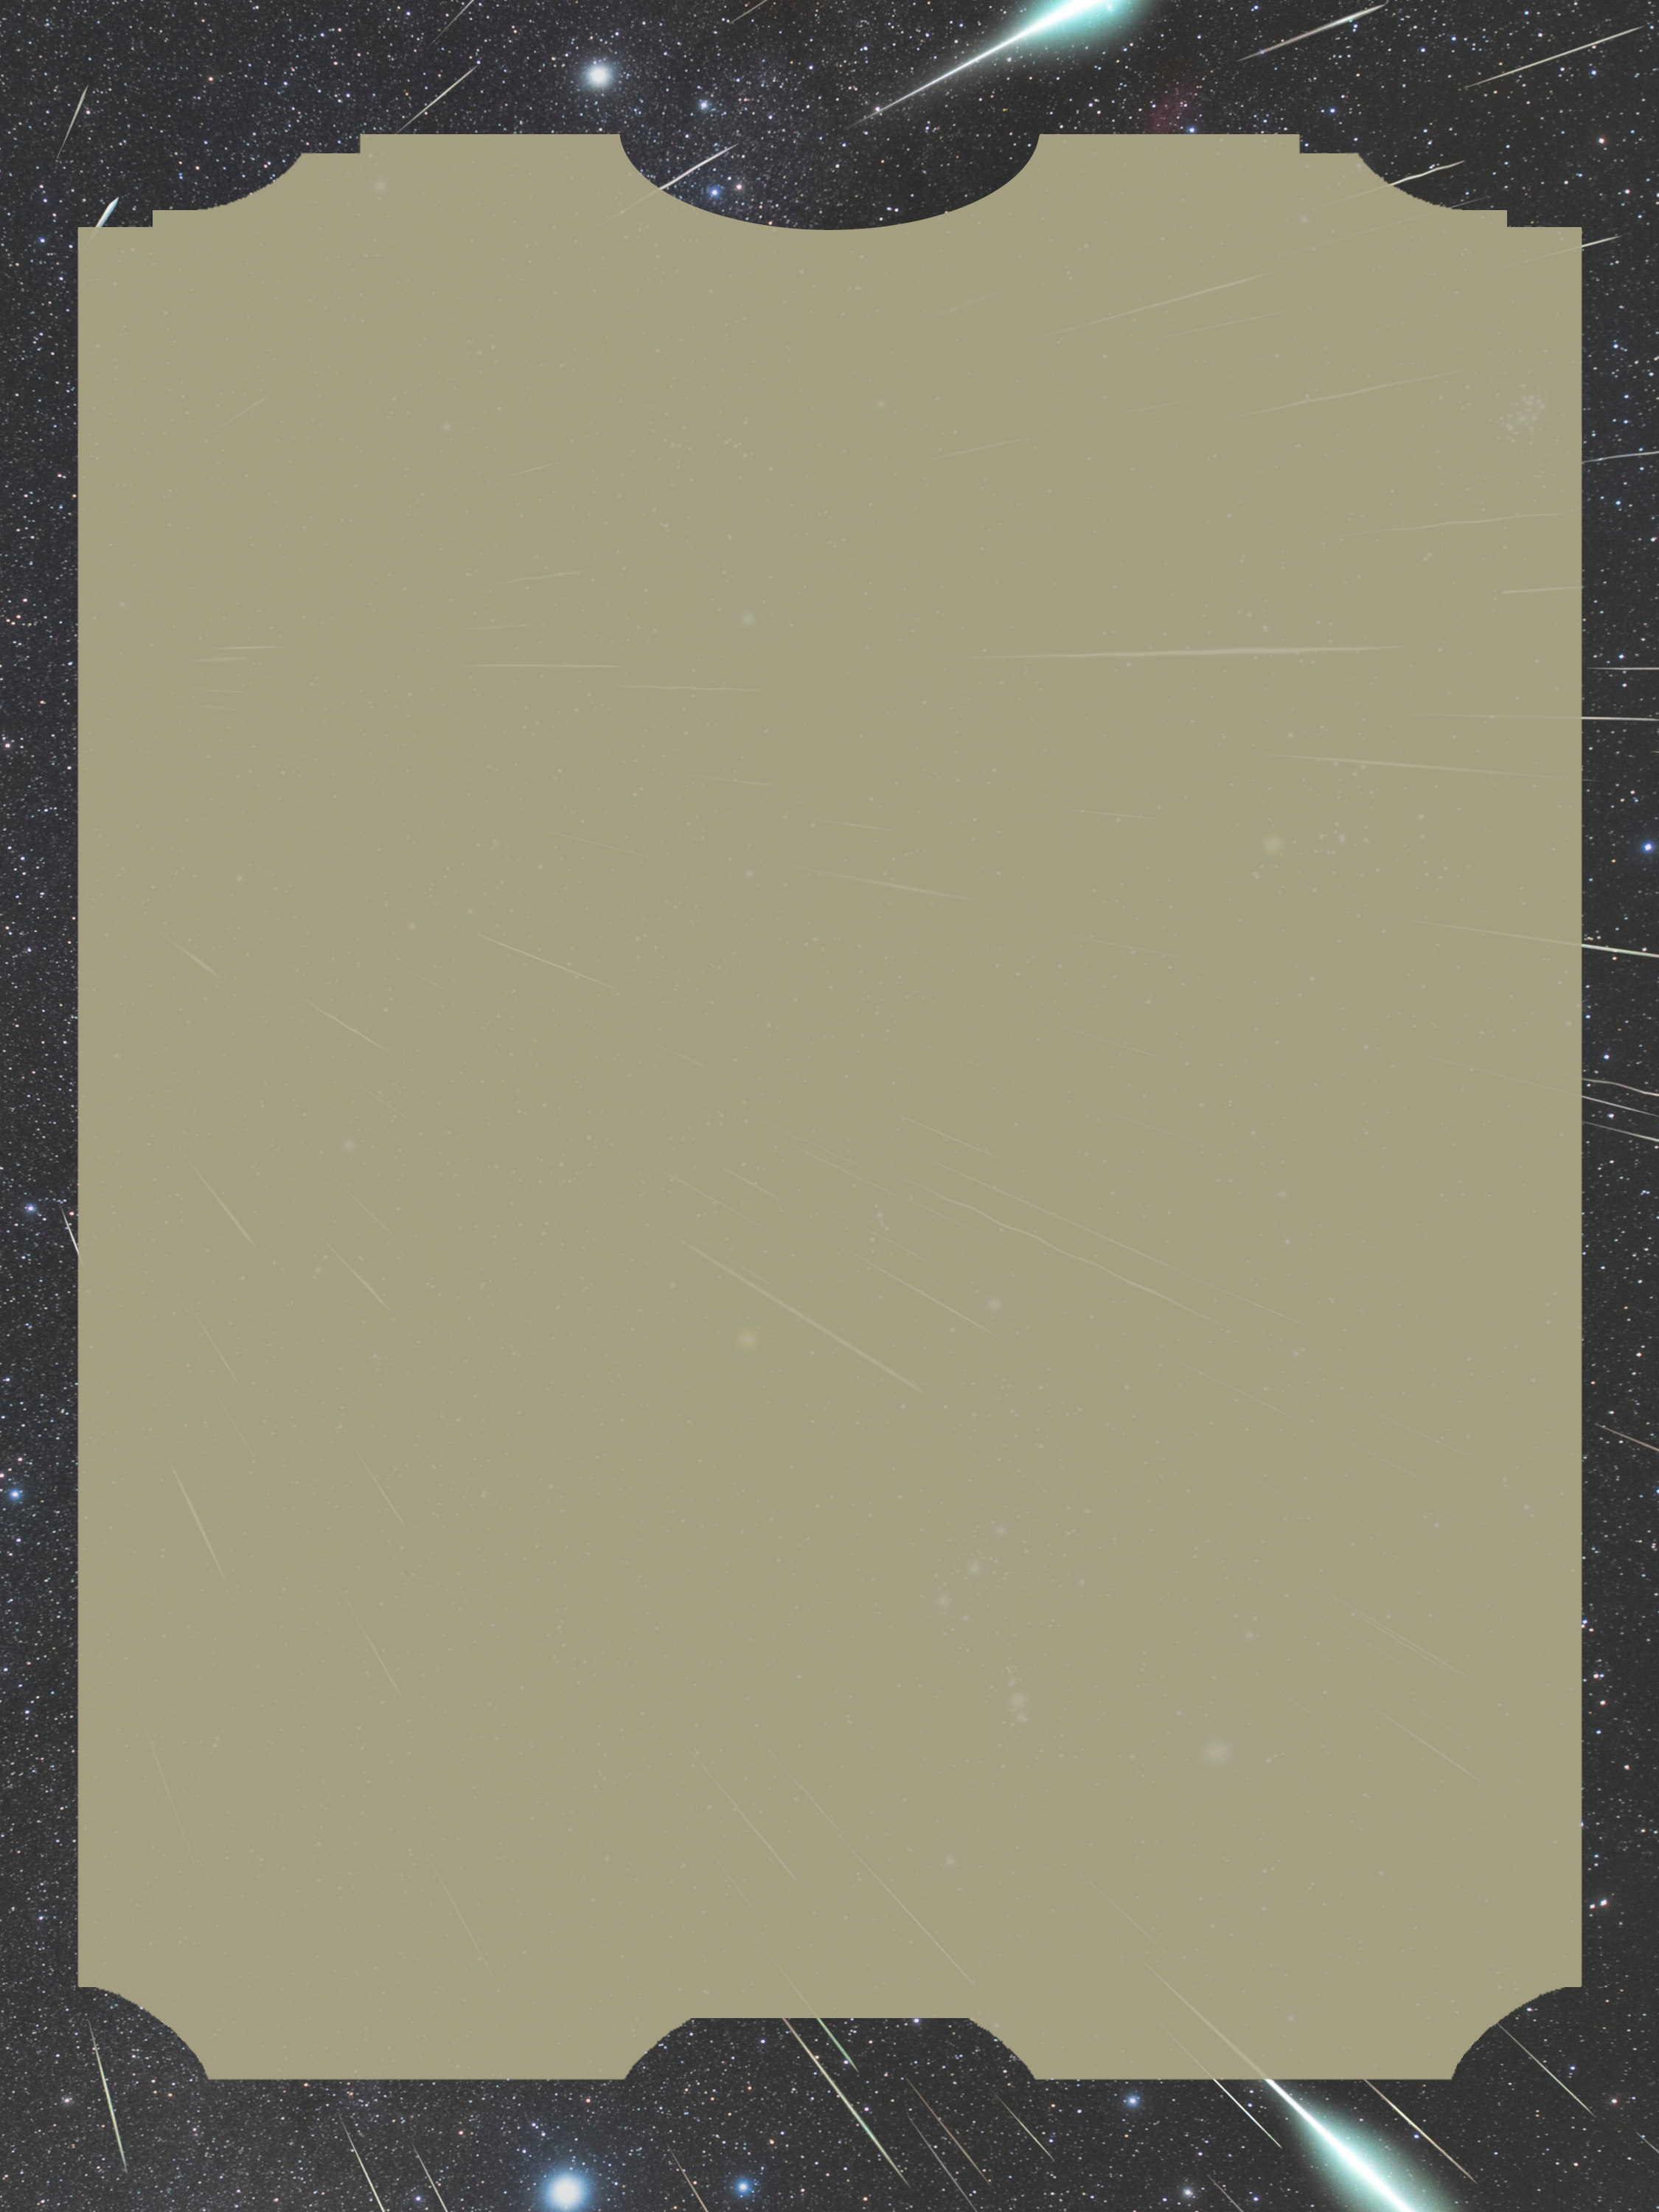
\includegraphics[width=\paperwidth,height=\paperheight]{meteors.jpeg}}
\renewcommand\thefootnote{{\color{myColor}{\arabic{footnote}}}}
\let\oldfootnote\footnote
    \renewcommand{\footnote}[1]{\oldfootnote{{\color{myColor}#1}}}
\begin{titlepage} % Suppresses headers and footers on the title page
	\centering % Centre everything on the title page
	%\scshape % Use small caps for all text on the title page

	%------------------------------------------------
	%	Title
	%------------------------------------------------
	
	\rule{\textwidth}{1.6pt}\vspace*{-\baselineskip}\vspace*{2pt} % Thick horizontal rule
	\rule{\textwidth}{0.4pt} % Thin horizontal rule
	
	\vspace{1\baselineskip} % Whitespace above the title
	
	{\scshape\Huge "Uber Feuer-Meteore,\\[1.25pt] und "uber die mit denselben\\[1.25pt] herabgefallenen Massen.\\[1.25pt]}
	
	\vspace{1\baselineskip} % Whitespace above the title

	\rule{\textwidth}{0.4pt}\vspace*{-\baselineskip}\vspace{3.2pt} % Thin horizontal rule
	\rule{\textwidth}{1.6pt} % Thick horizontal rule
	
	\vspace{1\baselineskip} % Whitespace after the title block
	
	%------------------------------------------------
	%	Subtitle
	%------------------------------------------------
	
	{\scshape Von Ernst Florens Friedrich Chladni,} % Subtitle or further description
	
	\vspace*{1\baselineskip} % Whitespace under the subtitle
	
    {\scshape\scriptsize der Philosophie und Rechte Doktor, der kaiserlich Akademie der Wissenschaften zu St. Petersburg, der k"oniglich Akademien zu Berlin, M"unchen und Turin, der k"oniglich Soziet"aten der Wissenschaften zu G"ottingen und zu Haarlem, der Gesellschaft naturforschender Freunde zu Berlin, der philomatischen zu Paris, der Gro"sherzoglich mineralogischen zu Jena, der Akademie der K"unste und Wissenschaften zu Livorno, der Gesellschaft f"ur Naturfunde zu Rotterdam, der Hamburgischen zu Bef"orderung der K"unste und n"utzlichen Gewerbe, der naturforschenden Gesellschaft zu Halle, der naturhistorischen zu Hannover, und noch einiger andern teils Mitgliede, teils Korrespondenten.} % Subtitle or further description
    
	%------------------------------------------------
	%	Editor(s)
	%------------------------------------------------
    \vspace*{\fill}

	\vspace{1\baselineskip}

	{\small\scshape Wien 1819.}
	
	{\small\scshape{Im Verlage den J. G. Heubner.}}
	
	\vspace{0.5\baselineskip} % Whitespace after the title block

    \scshape Internet Archive Online Edition  % Publication year
	
	{\scshape\small Namensnennung Nicht-kommerziell Weitergabe unter gleichen Bedingungen 4.0 International} % Publisher
\end{titlepage}
\setlength{\parskip}{1mm plus1mm minus1mm}
\clearpage
\tableofcontents
\clearpage
\section*{Vorrede.}
\paragraph{}
Da das, herabfallen meteorischer Massen, und der kosmische Ursprung derselben, durch mich zuerst im Jahre 1794 unter den Physikern zur Sprache gebracht worden ist, so haben sp"aterhin Mehrere den Wunsch ge"au"sert, dass ich diesen Gegenstand mit Benutzung der neuern Beobachtungen und Untersuchungen mehr im Zusammenhange bearbeiten m"ochte. Einen besonderen Wert f"ur mich hatte hierbei die Aufforderung von Seiten des Herrn Doktor Olbers, in der monatlichen Korrespondenz des Freiherrn von Zach, Februar 1803, und aus dieser in Gilberts Annalen der Physik, B. 14, S. 45. Recht gern h"atte ich fr"uher diesem Wunsche Gen"uge geleistet, aber teils war ich mit andern Dingen besch"aftigt, die ich doch auch nicht vernachl"assigen wollte, oder durste, (z. B. mit alle dem, was zur Ausarbeitung meiner Neuen Beitr"age zu Akustik n"otig war, mit Vervollkommnung meines Klavizylinder, und mit Untersuchungen "uber die verschiedenen m"oglichen Bauarten solcher Instrumente); teils auch hatte ich hierzu den weiten noch nicht genug Beobachtungen zu sammeln Gelegenheit gehabt. Ich lie"s es also vor der Hand dabei bewenden, von Zeit zu Zeit Beitr"age in Gilberts Annalen und in anderen wissenschaftlichen Zeitschriften zu liefern. Erst im Mai 1816 fasste ich den festen Entschluss, etwas Ganzes hier"uber auszuarbeiten, und dieses bis zur geschehenen Ausf"uhrung als mein Hauptbestreben anzusehen, wozu die Reise, welche ich mir vorgenommen hatte, mir sehr beh"ulflich fein konnte und musste. Da n"amlich dieser Gegenstand unter die Dinge geh"ort, welche sich nicht \emph{a priori} konstruieren (wof"ur mir im Deutschen kein anderer Ausdruck sogleich beifallen will als: aus den Fingern saugen) lassen, und wo man, so viel als m"oglich, alle vorhandenen Beobachtungen beisammenhaben muss, um nicht einseitig "uber die Sache zu urteilen; so habe ich auf dieser Reise weder M"uhe noch Kosten gescheut, um alle Beobachtungen, deren ich habhaft werden konnte, zu sammeln. In dieser Absicht blieb ich zwei Monate in Gotha, und drei Monate in G"ottingen, um in den dortigen Bibliotheken alles hierher Geh"orende nachzusehen; benutzte besonders in Hamburg, Bremen und Wien viele ausl"andische Zeitschriften; machte im Julius 1818 eine Exkursion von Karlsruhe nach Paris, um in den dortigen Bibliotheken und Naturalien-Kabinetten manches nachzusehen u. s. w., so dass ich wissentlich nichts von dem, was zur Sache geh"ort, vernachl"assigt habe. Um dem Buche die geh"orige Korrektheit zu geben, bin ich bis nach Beendigung des Druckes in Wien geblieben. "Ubrigens halte ich f"ur n"otig (weil man mich "ofters darum befragt hat) die Bemerkung beizuf"ugen, dass alles, was ich bei dieser Gelegenheit, und auch sonst, f"ur Naturkenntnisse, und bei den akustischen Untersuchungen auch f"ur deren Anwendung auf Kunst, zu tun mich bestrebt habe, auf meine eigene Rechnung geschehen ist, indem ich von Niemanden irgendeinen Gehalt oder andere Vorteile genie"se.

Jedem, der sich durch Lieferung brauchbarer Nachrichten, oder sonst auf irgendeine Art um die Sache verdient gemacht hat, habe ich gern am geh"origen Orte Gerechtigkeit widerfahren lassen. Alle die Schriften, welche Beobachtungen von Tatsachen enthalten, habe ich zu benutzen, und immer aus den ersten Quellen zu sch"opfen mich bestrebt; viele Schriften aber, die blass Meinungen und Urteile enthalten, habe ich nicht angef"uhrt, weil hier nicht die Absicht war, eine vollst"andige Literatur des Gegenstandes zu liefern, sondern den Gegenstand selbst abzuhandeln. Es liegt auch nicht viel daran, zu wissen, wie dieser oder jener sich die Sache vorstellt, wohl aber zu wissen, was beobachtet worden ist, und was aus den Beobachtungen, mit Zuziehung bekannter Naturgesetze, auf die einfachste und nat"urlichste Art folgt. Hierbei kommt auch gar nichts darauf an, ob eine Behauptung alt oder neu ist, oder auch, ob sie Manchem, der in seinen einmal gefassten Vorstellungen nicht gern etwas ab"andert, und alles auf einen gar zu engen Kreis zu beschr"anken geneigt ist,\footnote{Viele, denen es sonst nicht an Einsichten fehlt, haben eine besondere Scheu daf"ur, sich so manches im Weltall so gro"s zu denken, als es wirklich ist, und "uberhaupt sich die Dinge in ihrer wahren verh"altnism"a"sigen Gr"o"se oder Kleinheit vorzustellen. Viele m"ochten auch gar gern unsern gegen so viele andere Weltk"orper sehr kleinen Erdball (und vielleicht auch auf diesem ihr liebes Ich) als das Wichtigste im Weltall ansehen, um dessentwillen alles "Ubrige da ist, und worauf sich Alles bezieht. Solche m"ussten eigentlich, wenn sie recht konsequent fein wollen, Anh"anger des ptolem"aischen oder des tychonischen Systems fein und bleiben. Wirklich habe ich auch vor vielen Jahren zwei sonst verst"andige M"anner gekannt, die physikalische und mathematische Kenntnisse hatten, oder zu haben glaubten; von denen aber der Eine dem ptolem"aischen, der Andere dem tychonischen Welt-Systeme mit sehr vielem Eifer anhing, weil sie, wie vormals Galileis Gegner, es f"ur "au"serst s"undlich und verderblich hielten, wenn man ann"ahme, dass die Erde sich bewege. Beide gaben sich alle M"uhe, um mich von ihrer Meinung zu "uberzeugen; ich antwortete ihnen aber, mir k"ame das, wenn man nur noch einen Schritt weiter in das Kleine gehen wollte, ungef"ahr so vor, als ob, wenn ein Hase gebraten w"urde, man annehmen wollte, dass nicht etwa der Hase nebst dem Spie"se sich bewege, sondern dass die K"uche nebst dem Feuer, so wie auch das ganze Haus, die Erde, und allenfalls auch das ganze Weltall sich um den Hafen drehe, damit er gebraten werde.} etwa gar zu paradox vorkommen m"ochte. Jeder Satz, der etwas zur Vermehrung unserer Kenntnisse beigetragen hat, war einmal zu irgendeiner Zeit etwas Ungew"ohnliches oder Paradoxes, und musste also Manchem zum Ansto"s gereichen; h"atte man also immer bei dem Gew"ohnlichen wollen stehen bleiben, so w"aren alle menschlichen Kenntnisse und Einrichtungen noch in dem Zustande der ersten Kindheit oder Rohheit, oder w"aren wenigstens sehr langsam vorw"artsgeschritten.

Herr v. Schreibers, Direktor der k. k. Hof-Naturalien-Kabinette in Wien, welcher sich um die Lehre von den Meteor-Massen in mehreren Hinsichten sehr verdient gemacht hat, fand f"ur gut, diesem Buche eine Beilage von 10 Steindruck-Tafeln, nebst deren Erkl"arung, beizuf"ugen, welche ein besonderes Heft in 4 $^\wedge$10 ausmacht, und worin verschiedene im k. k. Naturalien-Kabinette befindliche Meteor-Massen und Figuren auf ge"atzten Fl"achen einiger Arten des Meteor-Eisens dargestellt werden, so wie auch die Gegend um Stannern, auf welche am 22. Mai 1808 Meteor-Steine fielen. Diese kleine Karte ist ein Gegenst"uck zu der, welche Biot von der Gegend um L'Aigle geliefert hat, wo die Meteor-Steine am 26. April 1803 ebenfalls auf einen elliptischen Bezirk gefallen sind. Ich zweifle gar nicht, dass es den Lesern angenehm sein werde, wenn sie dadurch einen anschauenden Begriff von Machen in diesem Buche beschriebenen Gegenst"anden erhalten k"onnen. Als Anhang zu dem Buche selbst hat er ein Verzeichnis der im k. k. Naturalien-Kabinette zu Wien befindlichen Sammlung von meteorischen Stein- und Eisen-Massen beigef"ugt, welche ohne Zweifel unter allen in Hinsicht der Mannigfaltigkeit sowohl, als der Prachtst"ucke, die vorz"uglichste ist. Die Bekanntmachung des Verzeichnisses war wohl notwendig, weil schon manches Unrichtige war dar"uber gesagt worden.

Da nun der Zweck, warum ich ungef"ahr seit drei bis vier Jahren die Bearbeitung der Lehre von den Meteor-Massen als Hauptsache angesehen habe, durch die Herausgabe dieses Buches, so gut es mir m"oglich war, er f"ullt ist, so gedenke ich nun wieder manche andere Dinge als Hauptbesch"aftigung anzusehen, und auch wieder einmal weitere Untersuchungen "uber die Bauarten der beiden von mir erfundenen Instrumente, des Klavizylinders und des Euphon, anzustellen, wovon vorz"uglich ersteres seht verschiedener Arten der Einrichtung, und betr"achtlicher Vervollkommnungen f"ahig ist, und einmal in der Folge, wenn es in mehrerer Vollkommenheit, als jetzt, allgemeiner verbreitet werden sollte, vieles w"urde dazu beitragen k"onnen, Manchem mehreren Geschmack an harmonischen und gebundenen S"atzen beizubringen, als an solchen, wo es blo"s auf Fertigkeit ankommt. Was ich dar"uber, um nichts verloren gehen zu lassen, vor einigen Jahren nebst den n"otigen Zeichnungen schriftlich aufgesetzt habe, ist nach meinen jetzigen Begriffen noch gar zu unreif, und es sind noch weit mehrere Forschungen und Experimente n"otig, um vielleicht auch "uber diesen Gegenstand einmal in der Folge etwas Ganzes zu liefern. Auch fehlt es sonst nicht an Stoff zur Besch"aftigung, und an Luft dazu wird es mir, so lange ich mich so gesund f"uhle, wie bisher, hoffentlich auch nicht fehlen. "Ubrigens, von welcher Art auch meine Besch"aftigungen sein m"ogen, werde ich doch auch nicht unterlassen, auf alles das aufmerksam zu sein, was die Geschichte und die weitere Kenntnis des hier bearbeiteten Gegenstandes betrifft, um in der Folge Nachtr"age zu dem, was hier gesagt ist, zu liefern. Sollte etwa ein und anderer Leser dieses Buches Gelegenheit haben, mir glaubw"urdige Nachrichten mitzuteilen, welche weder hier, noch in einer bekannten Zeitschrift erw"ahnt sind, von merkw"urdigen Feuer-Meteoren, von Stein- und Eisen-Niederf"allen, von Gediegeneisen-Massen, die auch f"ur meteorisch zu halten sind, von Niederf"allen staubartiger, schlammiger oder bitumin"oser Stoffe,\footnote{Denjenigen, welche etwa Gelegenheit haben, einen Staubniederfall, oder das Herabfallen einer schleimigen Materie mit einer sternschnuppenartigen Lichterscheinung (wovon mir au"ser den in der sechsten Abteilung erw"ahnten Beispielen noch viele andere, aber zu unbestimmt, als dass sie hier h"atten k"onnen mit angef"uhrt werden, von glaubw"urdigen Personen erz"ahlt worden sind, und wo in dem einen Falle der zum Teil auf ein Kleidungsst"uck gefallene schleimige Stoff noch am folgenden Tage phosphoresziert haben soll); ist sehr zu empfehlen, des sie so viel als m"oglich von dem herabgefallenen Stoffe, oder wenn es roter Regen oder Schnee ist, von dem Bodensatze desselben sammeln, und irgendjemanden, der physikalische und chemische Untersuchungen dar"uber anstellen kann, zukommen lassen, indem diese Stoffe bis jetzt weit weniger untersucht worden sind, als die herabgefallenen Stein- und Eisenmassen. Wenn der Beobachter auch sein Physiker, aber doch sonst verst"andig und gebildet ist, so wird er doch wohl, sobald er einmal auf die Sache aufmerksam gemacht worden ist, f"ur billig erachten, aus Liebe f"ur die Wissenschaft sich einer so geringen Bem"uhung zu unterziehen.} oder sollte etwa jemand so gef"allig sein wollen (wie schon Mancher gewesen ist), meine Sammlung meteorischer Substanzen durch irgendetwas von der Art, das ich noch nicht besitze, zu vermehren, so w"urde ich es mit allem geb"uhrenden Danke anerkennen, und ich w"urde in diesem Falle bitten, wenn der "Ubersender sich innerhalb der "Osterreichischen Monarchie befindet, durch die J. G. Heubner'sche Buchhandlung in Wien; wenn er sich aber au"serhalb derselben befindet, durch die Breitkopf- und H"artel'sche Buchhandlung in Leipzig, es (mit m"oglichster Ersparung des Porto, besonders wenn die Sache nicht von vorz"uglicher Wichtigkeit ist) an mich gelangen zu lassen.

Geschrieben im September 1819.

E. F. F. Chladni.
\clearpage
\section*{"Ubersicht des Inhalts.}
\subsection*{Erste Abteilung. Geschichte der ersten Untersuchungen des Niederfallens meteorischer Massen.}
\paragraph{}
§. 1. Die Alten kannten schon diese Art von Naturerscheinungen.

§. 2. Nachheriger Unglaube, der bis zur Verstockung ging, mit wenigen Ausnahmen.

§. 3. Der Verfasser war in neuerer Zeit der erste, der diesen Unglauben bek"ampfte.

§. 4. Veranlassung dazu.

§. 5. Fortdauer des Unglaubens, und Anfechtungen, die der Verfasser sich musste gefallen lassen.

§. 6. Einige Ausnahmen in Deutschland.

§. 7. Untersuchungen in England.

§. 8. Etwas sp"aterer Glaube, und weitere Untersuchungen in Frankreich.

§. 9. Endliche allgemeine Anerkennung.
\subsection*{Zweite Abteilung. Allgemeine Bemerkungen "uber Feuerkugeln, und "uber den herabgefallenen Massen.}
\paragraph{}
§. 1. Allgemeiner Begriff von dieser Art der Naturerscheinungen.

§. 2. Anfang der Erscheinung eines solchen Meteors.

§. 3. Beobachtete H"ohe der Feuerkugeln.

§. 4. Beschaffenheit der Bahn. Achsendrehung. Bogenspr"unge. (Nebst einem sp"ateren Nachtrage zu Ende dieser Abteilung.)

§. 5. Geschwindigkeit der Bewegung.

§. 6. Gr"o"se der Feuerkugeln.

§. 7. Gestalt dieser Meteore.

§. 8. Licht und Farben derselben.

§. 9. Brennen, Rauch und Dampf.

§. 10. Zerplatzung der Feuerkugeln, mit Ersch"utterung und Get"ose.

§. 11. Dauer der Erscheinung.

§. 12. Niederfallen der Massen, welche entweder Meteor-Steine, oder Gediegeneisenmassen, oder auch staubartige, oder weiche Substanzen sind.

§. 13. Beschaffenheit der Meteor-Steine im Allgemeinen.

§. 14. Bestandteile derselben.

§. 15. Gr"o"se und Quantit"at der gefallenen Steine.

§. 16. Gestalt der Meteor-Steine.

§. 17. Rinde derselben.

§. 18. Beschaffenheit der Steinart.

§. 19. Meteorische Gediegeneisen-Massen.

§. 20. Niederf"alle von staubartigen oder weichen Substanzen in trockner oder feuchter Gestalt.

§. 21. "Uber noch manche anderen Dinge, die herabgefallen sein sollen.

§. 22. Die Feuerkugeln und die Niederf"alle meteorischer Massen sind von alle dem, was sich auf unsere Erde bezieht, unabh"angig.

§. 23. Unabh"angigkeit von Jahreszeiten.

§. 24. Unabh"angigkeit von Tageszeiten.

§. 25. Unabh"angigkeit von den Weltgegenden.

§. 26. Unabh"angigkeit von der geographischen Lage.

§. 27. Unabh"angigkeit vom Wetter.

§. 28. Unabh"angigkeit von Perioden.

§. 29. "Uber Schaden, der durch solche Meteore ist verursacht worden.

§. 30. Vergebliche Bem"uhungen des Verfassers, verschiedene "altere Meteor-Massen aufzufinden.

§. 31. "Ubereinkunft der Sternschnuppen mit den Feuerkugeln. (Nebst einem sp"ateren Nachtrage zu Ende der siebenten Abteilung.)

§. 32. Verzeichnis der Sammlung von Meteor-Substanzen, welche der Verfasser gegenw"artig besitzt. (Nebst einem sp"ateren Nachtrage zu Ende der sechsten Abteilung.)

§. 33. Wahrscheinlichkeit eines h"aufigen Niederfallens meteorischer Massen auf unsern Weltk"orper. (Sp"aterer Nachtrag zu §. 4.)

\subsection*{Dritte Abteilung. Nachrichten von beobachteten Feuerkugeln, und zwar sowohl von solchen, deren Massen man habhaft geworden ist, als auch von andern, in chronologischer Ordnung. Mehr als 280.}

\subsection*{Vierte Abteilung. Nachrichten von den Stein- und Eisenmassen, deren Niederfallen beobachtet worden ist, in chronologischer Ordnung.}
\subsubsection*{1. Vorerinnerungen.}
\subsubsection*{2. Niederf"alle von Stein- und Eisenmassen, vor unserer Zeitrechnung.}
\begin{center}
A. Wo sich die Zeit des Falles mehr oder weniger genau angeben l"asst. 
\end{center}
\begin{itemize}\small
    \item ? Ungef"ahr 1478 Jahre vor Christi Geburt, ein Stein in Kreta.
    \item ((Die Erz"ahlung von herabgefallenen Steinen im Buche Josua scheint von Hagel zu verstehen zu sein.))
    \item ? 1403 vor unserer Zeitrechnung, vielleicht eine Eisenmasse auf dem Ida.
    \item 1200, Steine bei Orchomenos.
    \item ? 705 oder 704, das Ancyle, wahrscheinlich eine Eisenmasse.
    \item 654, Steine auf dem albanischen Berge.
    \item 644, in China.
    \item 465, ein gro"ser Stein bei Aegos-Potamos.
    \item Nicht lange vorher oder nachher, ein Stein bei Theben.
    \item ((In Piceno, vielleicht nur Hagel.))
    \item 211, ein Stein in China.
    \item 206 oder 205, Steine, wahrscheinlich in Italien.
    \item 192, ein Stein in China.
    \item 176, ein Stein in den See des Mars, in agro Crustumino.
    \item 90 oder 89, Steine zu Rom.
    \item 89, Steine in China.
    \item 56 oder 52, Eisen in Lukanien.
    \item ((Bei Acilla vielleicht nur Hagel.))
    \item 38, 29, 22, 19, 12, 9, 6, 6, Steine in China.
\end{itemize}
\begin{center}
B. Wo sich die Zeit des Falles nicht bestimmen l"asst.
\end{center}
\begin{itemize}\small
    \item Der Stein aus Pessinus in Phrygien.
    \item Der Elagabal zu Emisa in Syrien.
    \item Ein Stein zu Abydos.
    \item Einer zu Cassandria oder Potidaea.
    \item ? Wahrscheinlich das Symbol der Diana zu Ephesus.
    \item ? Wahrscheinlich der Stein in der Kaaba zu Mekka, und noch einer, der dort aufbewahrt wird.
\end{itemize}
\subsubsection*{3. Niederf"alle von Stein- und Eisenmassen, nach dem Anfange unserer Zeitrechnung.}
\begin{itemize}\small
    \item In der ersten H"alfte des ersten Jahrhunderts ein Stein in Vocontiorum agro.
    \item In den Jahren 2, 106, 154, 310 und 333, Steinf"alle in China.
    \item ((Ein angeblicher Niederfall im Jahre 416 ist ein Missverst"andnis.))
    \item 452, Steine in Thrakien.
    \item Sp"aterhin ein Stein bei Emessa in Syrien, und auch einige auf dem Berge Libanus.
    \item ? Vielleicht um 570, Steine bei Beder in Arabien.
    \item 616, Steine in China.
    \item ? 648, ein gro"ser Stein zu Konstantinopel.
    \item (Einige nicht einzuschaltende angebliche Niederf"alle.)
    \item ? 839, Steine in Japan.
    \item 852, ein Stein in Tabaristan.
    \item 856, Steine in "Agypten.
    \item ? 885, Steine in Japan.
    \item 897, Steine bei Kufah.
    \item 951, ein gro"ser Stein bei Augsburg.
    \item 998, Steine bei Magdeburg.
    \item Bald nach 1009, eine Eisenmasse bei Dschordschan.
    \item ((Ein angeblich bei Cordova gefallener Stein scheint eine Verwechselung mit der vorigen Begebenheit zu sein.))
    \item 1021, Steine in Afrika.
    \item ((Eine fabelhafte Nachricht von einem bei Jerusalem gefallenen Steine.))
    \item 1057, Steine in Corea.
    \item 1112, Steine oder vielleicht Eisenmassen bei Aquileja.
    \item 1135 oder 1136, ein Stein zu Oldisleben in Th"uringen.
    \item ? 1138, vielleicht ein Steinfall zu Mosul.
    \item 1164, Eisen im Mei"snischen.
    \item ((Einige Ereignisse, die nicht scheinen unter die Steinf"alle zu geh"oren.))
    \item 1249, Steine bei Quedlinburg und an anderen Orten.
    \item ? In dieselben Jahrhunderte vielleicht ein Stein in W"urzburg.
    \item Zwischen 1251 und 1360, Steine bei Welikoi-Ustiug.
    \item 1280, eine Stein- oder Eisenmasse bei Alexandria in "Agypten.
    \item 1304, viele Steine oder Eisenmasse bei Friedland oder Friedeburg.
    \item ? 1328, vielleicht Steine in Mortahiah und Dakhaliah.
    \item ? 1339, vielleicht Steine in Schlesien.
    \item ? 1368, wahrscheinlich eine Eisenmasse im Oldenburgischen.
    \item 1379, Steine zu Minden.
    \item 1421, ein Stein auf der Insel Java.
    \item ? 1438, viele leichte Steine bei Roa in Spanien.
    \item ? Wahrscheinlich in dieselben Jahrhunderte ein Stein bei Lucern.
    \item 1491, ein Stein bei Rivolta de' bassi, nicht weit von Crema.
    \item 1492, ein gro"ser Stein bei Ensisheim.
    \item 1496, Steine bei Cesena und Forli.
    \item ? Wahrscheinlich in dieselben Jahrhunderte, oder nicht lange darnach, ein Stein bei Br"ussel.
    \item ((Verschiedene nicht einzuschaltende angebliche Steinf"alle.))
    \item 1511, gro"ser Steinfall bei Crema.
    \item 1516, Steine in China.
    \item 1520, Steine in Aragon, zwischen Oliva und Gandia.
    \item ? 1528, Steine bei Augsburg.
    \item ? 1540, ein gro"ser Stein in Limousin.
    \item Ungef"ahr zwischen 1540 und 1550, eine Eisenmasse im Walde bei Naunhof.
    \item Um die Mitte dieses Jahrhunderts, Eisen an mehreren Orten in Piemont.
    \item 1552, viele Steine bei Schleusingen u. s. w.
    \item 1559, Steine bei Miskolz in Ungarn.
    \item 1561, Steine oder Eisen, bei Torgau und Eilenburg.
    \item ((1564, ein angeblicher Steinfall zwischen Mecheln und Br"ussel, scheint eine Erdichtung zu sein.))
    \item ? 1572, vielleicht Steine bei Thorn.
    \item 1580, gro"ser Steinfall bei N"orten, nicht weit von G"ottingen.
    \item 1581, ein Stein bei Niederreissen in Th"uringen.
    \item 1583, ein Stein bei Castrovillari in Abruzzo.
    \item 1583, einer in Piemont.
    \item 1596, Steine zu Crevalcote.
    \item Wahrscheinlich in dieselben Jahrhunderte ein Stein im K"onigreiche Valencia in Spanien.
    \item 1618, gro"ser Steinfall in Steiermark.
    \item 1618, eine metallische Masse in B"ohmen.
    \item 1621, eine Eisenmasse bei Lahore in Indien.
    \item 1622, ein Stein in Devonshire.
    \item 1628, ein Stein bei Hatford in Berkshire.
    \item 1634, Steine in der Grafschaft Charollois.
    \item ? 1635, ein Stein bei Calce im Vicentinischen.
    \item 1636, ein gro"ser Stein zwischen Sagan und Dubrow in Schlesien.
    \item 1637, ein Stein auf dem Berge Vaisien in der Provence.
    \item 1642, einer in Suffolk.
    \item 1643 oder 1644, Steine auf ein Schiff im Ostindischen Meere.
    \item 1647, ein Stein bei Zwickau.
    \item 1647, ein Stein bei Stolzenau in Westphalen.
    \item ? Zwischen 1647 und 1654, ein Stein im Ostindischen Meere.
    \item 1650, ein Stein in Dordrecht.
    \item 1654, gro"ser Steinfall auf der Insel F"unen.
    \item Ungef"ahr nach der Mitte dieses Jahrhunderts, ein gro"ser Stein in Warschau.
    \item Desgleichen ein kleiner Stein in Mailand.
    \item ((Eine unglaubliche Nachricht von gefallenen Steinen in Schiras, 1667, nebst zwei "ahnlichen Nachrichten.))
    \item 1668, gro"ser Steinfall bei Verona.
    \item 1671, Steine in der Ortenau in Schwaben.
    \item ? 1673, bei Dietlingen im Badenschen.
    \item 1674, Steine im Canton Glarus.
    \item Zwischen 1675 und 1677, ein Stein auf ein Schiff beider Insel Copinsha.
    \item 1677, Steine in Ermendorf bei Gro"senhain.
    \item 1680, in London.
    \item 1697, bei Siena.
    \item 1706, einer bei Larissa in Griechenland.
    \item 1722, Steine bei dem Kloster Schefftlar im Freisingischen.
    \item 1723, bei Plescowitz in B"ohmen.
    \item ((Ein angeblicher Niederfall bei Lessai ist nur ein Missverst"andnis.))
    \item 1738, Steine in der Grafschaft Avignon.
    \item 1740, bei Hasargrad oder Rasgrad an der Donau.
    \item ((Ein angeblich in Gr"onland gefallener Stein war ein herabgerolltes Felsenst"uck.))
    \item 1750, ein Stein bei Coutances.
    \item 1751, Eisenmassen bei Agram.
    \item 1753, viele Steine bei Tabor in B"ohmen.
    \item 1753, Steine bei Laponas in Bresse.
    \item 1755, ein Stein bei Terranova in Kalabrien.
    \item 1766, einer bei Alboreto, nicht weit von Modena.
    \item ? 1766, einer zu Novellara.
    \item 1768, ein Stein bei Lucé.
    \item 1768, einer bei Maurkirchen im Innviertel.
    \item 1773, ein Stein bei Sigena in Aragon.
    \item 1775, einer bei Rodach in Koburgischen.
    \item 1775 oder 1776, Steine bei Obruteza in Volhynien.
    \item 1776 oder 1777, bei Fabbriano.
    \item 1779, ei Pettiswood in Irland.
    \item 1780, bei Beefton in England.
    \item 1782, ein gro"ser Stein bei Turin.
    \item 1785, Steinfall im Eichst"adtischen.
    \item 1787, im Gouvernement von Charkow.
    \item 1790, gro"ser Steinfall bei Barbotan, u. s. w.
    \item 1791, Steine bei Castel-Berardenga in Toskana.
    \item 1791, bei Menabilly in Cornwallis.
    \item 1794, sehr viele Steine bei Siena.
    \item 1795, Steine in Ceylon.
    \item 1795, ein Stein in Yorkshire.
    \item 1796, bei Belaja Zerkwa im s"udlichen Russland.
    \item 1796, einer in Portugal.
    \item 1798, einer bei Salles im Rhone-Departement.
    \item 1798, Steine bei Benares in Bengalen.
    \item 1801, auf der île des tonneliers.
    \item 1802, in den schottischen Hochlanden.
    \item 1803, gro"ser Steinfall bei L'Aigle.
    \item 1803, Steinfall bei East-Norton in England.
    \item 1803, ein Stein bei Apt, im Departement de Vaucluse.
    \item 1803, einer bei Eggenfelde im Innviertel.
    \item 1804, bei High-Possil in Schottland.
    \item Ein Stein in Dorbrecht.
    \item 1805, Steine bei Doroninsk in Sibirien.
    \item 1805, zu Konstantinopel.
    \item 1806, Steine, von andern verschieden, bei Alais, im Departement du Gard.
    \item 1806, ein Stein bei Basingstoke in Hantshire.
    \item 1807, ein gro"ser Stein bei Timochin im Gouvernement von Smolensk.
    \item 1807, viele Steine bei Weston in Connecticut.
    \item 1808, Steine im Parmesanischen.
    \item 1808, gro"ser Steinfall bei Stannern in M"ahren.
    \item 1808, Steine bei Lissa in B"ohmen.
    \item ? 1809, bei Nord-Amerika auf ein Schiff und in das Meer.
    \item 1810, in Caswell-County in Neu-Connecticut.
    \item 1810, bei Shabad in Indien.
    \item 1810, in der Grafschaft Tipperary, in Irland.
    \item 1810, in der Gegend von Charsonville bei Orléans.
    \item 1810, ein Stein im Gouvernement von Poltawa.
    \item 1811, Steine bei Berlanguillas in Spanien.
    \item 1812, bei Toulouse.
    \item 1812, bei Erxleben, zwischen Magdeburg und Helmst"adt.
    \item 1812, bei Chantonnay im Departement de la Vendee.
    \item 1813, Steine bei Cutro in Kalabrien, mit gro"sem Staubniederfalle.
    \item ? 1813, Steine bei Malpas, nicht weit von Chester.
    \item 1813, in der Grafschaft Limerick in Irland.
    \item 1814, ein Stein bei Bachmut in Russland.
    \item 1814, Steine bei Sawotaipola, nicht weit von Friedrichshamm, in Finnland.
    \item 1814, bei Agen, im Departement du Lot et Garonne.
    \item 1814, bei Doab in Indien.
    \item 1815, bei Chassigny nicht weit von Langres.
    \item 1816, bei Glastonbury in Sommersetshire.
    \item 1818, einer im Dorfe Slobodka, im Gouvernement von Smolensk.
\end{itemize}
\paragraph{}
 (Nacherinnerung zu dieser und zu der vorigen Abteilung, die in China beobachteten Feuer-Meteore und Steinf"alle betreffend.)
\subsection*{F"unfte Abteilung. "Uber Gediegeneisenmassen, die auch als meteorisch k"onnen angesehen werden, "uber deren Niederfallen aber keine Beobachtungen vorhanden sind.}
\subsubsection*{1. Allgemeine Bemerkungen "uber das Vorkommen des meteorischen Gediegeneisens, und "uber das Gef"uge desselben.}
\subsubsection*{2. Nickelhaltige Gediegeneisenmassen, von "astigem oder zelligem Gef"uge, mit Ausf"ullung der Zwischenr"aume mit Olivin, oder Peridot.}
\begin{itemize}\small
    \item Die in Sibirien gefundene und durch Pallas bekannt gewordene Masse.
    \item ? Ein St"uck Gediegeneisen aus B"ohmen.
    \item Ein St"uck, welches bei Eibenstock in Sachsen ist gefunden worden.
    \item Ein St"uck, angeblich aus Norwegen, im k. k. Naturalien-Kabinette zu Wien.
    \item Eine in Sachsen gefundene Masse, welche sich zu Gotha befindet.
\end{itemize}
\subsubsection*{3. Derbe nickelhaltige Eisenmassen, mit kristallinischem Gef"uge.}
\begin{itemize}\small
    \item (Die bei Agram 1751 gefallene, ist die einzige vorhandene, deren Niederfallen ist beobachtet worden.)
    \item Eine zu Elbogen in B"ohmen aufbewahrt gewesene Masse.
    \item Eine, die bei Lenarto in Ungarn ist gefunden worden.
    \item Eine Masse vom Vorgebirge der guten Hoffnung.
    \item Mehrere gro"se Massen am Senegal.
    \item In Mexico an verschiedenen Orten.
    \item ? Eine in Honduras.
    \item Eine bei San Iago del Estero in S"ud-Amerika, und noch eine nicht weit davon befindliche.
    \item Eine Masse in Brasilien, bei Bahia.
    \item Eine in Nord-Amerika bei Neu-Orléans gefundene Masse.
    \item Zwei Eisenmassen an der n"ordlichen K"uste der Baffinbai.
\end{itemize}
\subsubsection*{4. Problematische Gediegeneisen-Massen, die keinen Nickel enthalten, und nicht von dem Gef"uge, wie die vorigen sind, oder auch deren Beschaffenheit nicht genug bekannt ist, um "uber ihren Ursprung urteilen zu k"onnen.}
\begin{itemize}\small
    \item Eine in Achen.
    \item Eine im Mail"andischen bei Villa gefundene Masse.
    \item Eine von Gro"s-Kamsdorf, nicht weit von Saalfeld.
    \item Eine, so auf einem Berge bei Cilly, in Steiermark ist gefunden worden.
    \item Eine bei Bitburg, nicht weit von Trier, gefundene Masse.
    \item Eine von Florac im Departement de la Loire.
    \item Eine bei Leadhills gefundene Masse.
    \item ? Ein gro"ses Felsenst"uck im "ostlichen Teile von Asien.
    \item Sechste Abteilung. Nachrichten von herabgefallenen staubartigen oder weichen Materien, in trockner oder feuchter Gestalt, in chronologischer Ordnung.
    \item Ungef"ahr um 473, gro"ser Niederfall von schwarzem Staube, um Konstantinopel.
    \item 642, Staub um Konstantinopel, und anderw"arts roter Schnee.
    \item 743, Staubniederfall an mehreren Orten.
    \item Um die Mitte des neunten Jahrhunderts blutroter Staub, wahrscheinlich einerlei Begebenheit mit dem Falle einer dem Blute "ahnlichen Substanz zu Balk, ungef"ahr um 860.
    \item 869, desgleichen zu Brixen, vielleicht, mit einer Ver"anderung des Datum, mit dem vorigen einerlei Meteor.
    \item 929, zu Bagdad r"otlicher Sand mit einer Feuererscheinung.
    \item 1056, roter Schnee in Armenien.
    \item 1110, R"otung des Sees Van in Armenien, durch eine hineingefallene Feuerkugel.
    \item 1416, roter Regen in B"ohmen.
    \item ? Bei Lucern, wahrscheinlich in dieselben Jahrhunderte, herabfall einer dem Blute "ahnlichen Substanz, und eines Steines mit einem Feuer-Meteor.
    \item 1501, sogenannter Blutregen an mehreren Orten.
    \item 1543, roter Regen in Westphalen.
    \item 1548, Herabfall einer Fl"ussigkeit, wie geronnen Blut, nach Erscheinung einer explodierenden Feuerkugel, in Th"uringen oder im Mansfeldischen.
    \item 1557, zu Schlage in Pommern, Niederfall einer Substanz wie geronnen Blut.
    \item 1560 (?), roter Regen zu L"owen und Emden.
    \item 1560, roter Regen zu Lillebonne, mit einem Feuer-Meteor, welches ein Pulver-Magazin anz"undete.
    \item ? 1582, Niederfall einer Substanz, bei Menschenhaare, mit sonderbarem Get"ose, zu Rockhausen bei Erfurt.
    \item 1586, bei Verden, eine Rothe und schw"arzliche Substanz, mit einem Feuer-Meteor.
    \item 1623, roter Regen zu Stra"sburg.
    \item 1637, schwarzer Staub im Archipelagus und in Syrien.
    \item 1638, roter Regen bei Turnhout.
    \item 1642, Schwefelklumpen bei Magdeburg, u. s. w.
    \item 1643, sogenannter Blutregen zu Vaihingen und zu Weinsberg.
    \item 1645, bei Herzogenbusch.
    \item 1646, zu Br"ussel.
    \item 1652, zwischen Siena und Rom, eine schleimige Substanz einer Sternschnuppe.
    \item ? 1665, bei Laucha, Niederfall einer Substanz, wie blaue Seide.
    \item ? 1665, schwefelartiger Staub in Norwegen.
    \item 1678, roter Schnee bei Genova.
    \item ? 1686, eine schwarze papierartige Substanz in Kurland.
    \item ? 1689, roter Staub in Venedig, u. s. w.
    \item 1711, roter Regen in Schonen.
    \item 1718, gallertartige Materie, von einer Feuerkugel, auf der Insel Lethi.
    \item 1719, Staubniederfall auf die atlantischen Meere, mit Lichterscheinung.
    \item 1721, roter Schlammregen um Stuttgart, mit einem Meteor.
    \item ? Ein St"uck Schwefel in England.
    \item 1744, roter Regen zu Pier d'Arena bei Genova.
    \item 1755, Niederf"alle von schwarzem und rotem Staube an verschiedenen Orten.
    \item 1763, roter Regen im Herzogtume Cleve, und bei Utrecht.
    \item ? Eine schwammige Masse von Masse von einer Feuerkugel, bei Koblenz, ohne Bestimmung der Zeit.
    \item 1781, wei"slicher Staub in Sizilien.
    \item 1796, Niederfall eines bitumin"osen Stoffes von einer Feuerkugel, in der Ober-Lausitz.
    \item Sp"aterhin eine gallertartige Masse, von einem Klumpen Feuer herabgefallen, bei Krefeld.
    \item 1803, gro"ser Niederfall von rotem Staube und rotem Schnee in Italien.
    \item 1809, roter Regen im Venezianischen.
    \item 1810, roter Schnee bei Piacenza.
    \item 1813, gro"ser Niederfall von rotem Staube, nebst Meteor-Steinen, in Italien.
    \item 1814, gro"ser Niederfall von schwarzem Staube, mit Feuererscheinung, bei Canada.
    \item 1814, rote Erde, im Thale von Oneglia.
    \item 1814, Staub zugleich mit den in Doab gefallenen Steinen.
    \item ? 1815, gro"ser Staubniederfall in den s"udlichen ostindischen Meeren.
    \item 1816, roter Schnee im n"ordlichen Italien.
    \item Rother Schnee an der n"ordlichen K"uste der Baffinbai.
    \item Rother Schnee auf der Alpe Anceindaz in der Schweiz, am Fu"se der Diablerets.
\end{itemize}
\paragraph{}
(Sp"aterer Nachtrag zu dem 32. der zweiten und zu der f"unften Abteilung; eine Antike aus Pompei, die Meteor-Eisen zu sein scheint, betreffend.)
\subsection*{Siebente Abteilung. "Uber den Ursprung der herabgefallenen Massen.}
\paragraph{}
§. 1. Vormalige Meinungen von dem, was Feuerkugeln w"aren.

§. 2. Nachherige Meinungen von dem Ursprunge der herabgefallenen Massen.

§. 3. Die herabfallenden Massen sind kosmisch, das ist, sie kommen aus dem allgemeinen Weltraume zu uns.

§. 4. Das Dasein solcher im allgemeinen Weltraume sich bewegenden Massen, ist durch sehr viele Beobachtungen erwiesen.

§. 5. Diese Massen k"onnen Haufen von Ur-Materie sein, die vor ihrer Ankunft noch keinem gr"o"seren Weltk"orper zugeh"ort hatte, und scheinen von kometenartiger Beschaffenheit zu sein.

§. 6. Sie k"onnen auch Tr"ummer eines zerst"orten Weltk"orpers sein.

§. 7. Ein Ursprung aus Mond-Vulkanen ist zwar an sich nicht unm"oglich, aber doch sehr unwahrscheinlich.

§. 8. Die niedergefallenen Massen k"onnen schlechterdings nicht aus Bestandteilen der Atmosph"are gebildet sein.

§. 9. Sie k"onnen auch nicht von der Erde durch vulkanische Kr"afte in die H"ohe gehoben sein.

(Sp"aterer Nachtrag zu dem 31. der zweiten Abteilung, die Beobachtungen der Sternschnuppen betreffend.)

\subsection*{Als Anhang folgt ein Verzeichnis der im k. k. Naturalien-Kabinette zu Wien befindlichen meteorischen Stein- und Eisenmassen, vom Herrn Direktor von Schreibers.}
\clearpage
\subsection*{Berichtigungen und Verbesserungen.}
\paragraph{}
S. 11. Z. 13, anstatt 1812, ist zu lesen 1802.

S. 78. Z. 8, von unten anstatt Grafen v. Schwarzburg, l. F"ursten v. Schwarzburg.

S. 91. Z. 4, von oben, anstatt September, l. Dezember. Auf derselben Seite ist einzuschalten: 1812, den 5. August bei Chantonnay, "uber $1\frac{1}{2}$ Unze. 1813, den 10. September, bei Limerick, ein kleines St"uck.

S. 93. Z. 2, anstatt Fl"usse der Diablerets, l. Fu"se der Diablerets.

S. 205. Z. 12, anstatt \emph{tempestata}, l. tempestate.

S. 226. Z. 2, muss das Comma vor dem Worte: scheinbar, stehen.

S. 243. Z. 23, Nicorps wird von Mehreren Niort genannt.

S. 247. Z. 18 und 19, anstatt \emph{matrice virescente}, l. \emph{matrici virescenti}.

-- -- Z. 20, anstatt at l. ad.

-- -- Z. 24, anstatt affirmant l. asserunt.

S. 262. Z. 7 und 12, anstatt Kalkerde l. Talkerde.

S. 276. in der Note Z. 3, anstatt der Merwede l. de Merwede.

S. 278. Z. 17, anstatt herr"uhren l. herr"uhrten.

-- -- Z. 22, muss vor 1808 den 15. M"arz ein * stehen.

S. 315. Z. 11, anstatt Liniendurchschnitte l. Linien Durchschnitte.

S. 355. in der Note, anstatt Proprodukt l. Produkt.

S. 364. Z. 2, von unten, anstatt \emph{fulgore} l. \emph{fulgure}.

S. 404. in der Note, Z. 13, anstatt Anmerkung l. Bemerkung.

S. 405. Z. 5, anstatt bei welcher l. bei welchen.

S. 413. Z. 6, von unten, anstatt schiefen l. schiefern.

Die Besitzer oder Leser dieses Buches werden ersucht, besonders die auf S. 11, 91, 93, 262, und 315 bemerkten Fehler in Berichtigen.
\clearpage
\section{Erste Abteilung. Geschichte der ersten Untersuchungen des Niederfallens meteorischer Massen.}
\subsection{Die Alten kannten schon diese Art von Naturerscheinungen.}
\paragraph{}
Schon in den "alteren Zeiten zweifelte man nicht, dass bisweilen Stein- und Eisenmassen mit einem Feuer-Meteor vom Himmel fallen. Da es hier nicht die Absicht ist, diesen Gegenstand in antiquarischer Hinsicht genauer abzuhandeln, berufe ich mich deshalb auf die vierte Abteilung, wo viele "altere Nachrichten von dergleichen Ereignissen angef"uhrt werden. Bei den Griechen und R"omern ward mit dergleichen Steinen mancher Aberglaube getrieben, indem man sie als Symbole der G"otter ansah; indessen scheinen doch auch Manche bessere Begriffe davon gehabt zu haben. So scheint es z. B., dass Anaxagoras vor dem Falle eines gro"sen Steines bei Aegos Potamos schon gesagt habe, dass bisweilen solche Steine vom Himmel fallen; so hat auch Plutarch den Fall dieses Steines so gut beschrieben, als es in der damaligen Zeit zu verlangen war; so sagt auch Damaskus (in \emph{Photii bibliotheca graeca}, c. 242) ganz richtig, dass die \emph{baetylia} (Meteor-Steine) mit einer Feuerkugel herabgefallen sind, u. s. w. Auch die "alteren Chinesen haben uns mehrere Nachrichten dieser Art mit historischer Treue, und ohne etwas T"orichtes einzumengen, "uberliefert. In dem mittleren Zeitalter haben uns besonders arabische Schriftsteller manche Nachrichten von solchen Ereignissen hinterlassen, ohne unrichtige Urteile einzumengen; auch ist dieses in noch etwas sp"ateren Zeiten von manchen Chroniken-Schreibern und einigen Andern\footnote{So hei"st z. B. in dem Buche \emph{de meteoris}, welches dem Theophrastus Paracelsus zugeschrieben wird, S. 3. der Basler-Ausgabe von 1569, 8.: \emph{evidentissime constat, lapides naturales ex coelo decidisse pariter ac metalla, sed non aliud, quam ferrum, nec lapidis quam unica species}. Auch in der Schrift: \emph{de Podagricis, lib. 2.}, sagt er, dass Steine vom Himmel fallen.} geschehen.
\subsection{Nachheriger Unglaube, der bis zur Verstockung ging, mit wenigen Ausnahmen.}
\paragraph{}
Nun kam aber eine Zeit, wo man mehrere Fortschritte in der Naturkunde machte, und jetzt glaubte man auf einmal alles, was nicht zu einem selbstgemachten Leisten passte, wegwerfen und f"ur Torheit erkl"aren zu m"ussen. Es ist fast unbegreiflich, wie durch die so sehr mit einander "ubereinstimmenden Nachrichten aus "alteren und neueren Zeiten, von den mit einem Feuer-Meteore und mit vielem Get"ose herabgefallenen Stein- und Eisenmassen, die Physiker nicht fr"uher veranlasst worden sind, der Sache weiter nachzuforschen, und die vorhandenen Nachrichten geh"orig mit einander zu vergleichen, da sie alsdann bei einer unbefangenen Ansicht gar bald sich w"urden gen"otigt gesehen haben, das Niederfallen solcher Massen, die Erkl"arungsart sei, welche man wolle, doch wenigstens als eine historisch erwiesene Tatsache anzunehmen. Einige Physiker waren indessen wahrheitsliebend genug, die Tatsachen, wenn sie auch solche nicht geh"orig zu erkl"aren wussten, doch unbefangen zu erz"ahlen, wie z. B. Baudin, Professor in Pau, und St. Amans,\footnote{Diesen ging es ebenso, wie mir etliche Jahre sp"ater, indem es f"ur Torheit erkl"art ward. Der Bericht von Baudin, in der \emph{Decade philosophique}, wurde von den Herausgebern mit der eben nicht sehr philosophischen Bemerkung begleitet, dass man so unglaubliche Dinge lieber wegleugnen, als sich auf Erkl"arungen einlassen m"usse. "Uber den Bericht von St. Amans, und "uber die Urkunde, welche die Munizipalit"at zu Juliac abgefasst hatte, dr"uckt sich Bertholon im \emph{Journal des sciences utiles}, 1790, so aus: \emph{Si les lecteurs eurent dès-lors l'occasion de déplorer l'erreur de quelques particuliers, combien ne gémiront pas aujourd'huit en voyant une municipalité entière attester, consacrer en bonne forme ces mêmes bruites populaires qui ne peuvent qu'exciter la pitié, nous ne dirons pas seulement des physiciens, mais de tous les gens raisonnables}. (! Wer so mitleidig ist, verdient doch wohl auch selbst Mitleid. Er f"ugt hinzu:) \emph{Que pouvons nous ajouter a ce proces-verbal; toutes les reflexions qu'il suggere, se presentent d'elles memes au lecteur philosophe, en lisant cette attestation d'un fait evidemment faux, d'un phenomene physiquement impossible.} (!)} Professor in Agen, den gro"sen Steinfall im Jahre 1790; oder wohl auch mehrere Nachrichten von Steinf"allen zu sammeln, wie Tata und Soldani; manche Obrigkeiten waren auch so verst"andig, nach einem solchen Naturereignisse "uber die Nachrichten, welcher sie habhaft werden konnten, eine Urkunde in geh"origer Form abzufassen, ohne etwas hinein zu mengen, was einem Vorurteile "ahnlich sieht. Gew"ohnlich aber machte man sich die Sache dadurch am leichtesten, dass man, wenn neue Ereignisse dieser Art gemeldet wurden, lieber die Tatsachen verdrehte (wovon genug Beispiele in der Folge vorkommen werden), oder sie geradezu wegleugnete, als dass man sich die M"uhe genommen h"atte, genauere Untersuchungen anzustellen. Der Unglaube ging so weit, dass man sogar die meisten in "offentlichen Sammlungen aufbewahrt gewesenen Meteor-Massen weggeworfen hat,\footnote{Wie z. B. im Dresden, eine 1581 in Th"uringen, und eine 1647 bei Zwickau gefallene Masse; in Wien, vier bei Miskolz 1559 gefallene Massen; in Kopenhagen, einen von den 1654 auf der Insel F"uhnen gefallenen Steinen; in Bern, einen 1698 gefallenen, nebst der Urkunde; in Verona, zwei von den 1668 gefallenen, einer 300, und einer 200 Pfund schwer; und noch einen, der in einer Kirche ist aufbewahret worden. Diejenigen, welche aus Aufkl"arungs-Vandalismus diese Massen, die man jetzt mit Silber aufw"agen w"urde, weggeworfen haben, k"onnte man recht f"uglich mit den B"ucherverbrennern Tschihoang-ti, Scipio Africanus, und Omar, in eine Classe setzen. Vielleicht aber lie"se sich doch noch eine oder die andere dieser Massen in irgendeiner alten Polterkammer, unter andern ausgemerzten Sachen, wieder auffinden, wenn man recht nachsuchen wollte.} weil man bef"urchtete, sich l"acherlich zu machen, und f"ur unaufgekl"art gehalten zu werden, wenn man nur die M"oglichkeit der Sache zug"abe.
\subsection{Der Verfasser war in neuerer Zeit der erste, der diesen Unglauben bek"ampfte.}
\paragraph{}
Wahrscheinlich w"urde das Niederfallen meteorischer Massen noch jetzt nicht als historisch erwiesene Wahrheit allgemein anerkannt werden, wenn ich nicht in der (zu Riga und Leipzig in der Ostermesse 1794 in 4. erschienenen) Abhandlung: "Uber den Ursprung der von Pallas entdeckten Eisenmasse, und einige damit in Verbindung stehende Naturerscheinungen, von E. F. F. Chladni, die Naturforscher zuerst darauf aufmerksam gemacht, und wenn nicht bald darauf die Natur meine Behauptungen durch einige auffallende Ereignisse dieser Art unterst"utzt h"atte, wie z. B. ein Paar Monate nach Erscheinung meiner Schrift durch den bekannten Steinfall bei Siena, und sp"aterhin durch die in Yorkshire, in Ost-Indien, und bei L'Aigle, welche unter den vielen, seit der Zeit geschehenen Steinf"allen, am meisten beigetragen haben, um Manchem einen Glauben an die Sache beizubringen. Ich habe in dieser Schrift gezeigt, und zwar nicht als Hypothese, sondern als etwas nicht zu bezweifelndes:
\begin{enumerate}
    \item Dass "ofters Stein- und Eisenmassen vom Himmel gefallen sind, und dieses als eine historisch erwiesene Wahrheit anerkannt werden m"usse;
    \item dass dieses Ereignis identisch mit Feuerkugeln ist, und diese nichts anders, als eine solche brennende Masse sind;
    \item dass diese Massen kosmisch sind, d. i. Ank"ommlinge aus dem Weltraume, welche vorher der Erde und deren Atmosph"are fremd waren.
\end{enumerate}
\paragraph{}
Eine franz"osische "Ubersetzung dieser Abhandlung von Eugene Coquebert erschien im Jahre 1804, im \emph{Journal des mines}, Nr. 88 und 90.
\subsection{Veranlassung dazu.}
\paragraph{}
Die erste Veranlassung verdanke ich einer Unterredung mit Lichtenberg, wiewohl dieser damals noch nicht wusste, dass jemals feste Massen vom Himmel gefallen w"aren, und also hiervon bei ihm nicht die Rede sein konnte.\footnote{Noch nach dem Erscheinen meiner Abhandlung war die ganze Sache Lichtenbergen so fremdartig, dass er zu Hrn. Prof. Harding und zu Andern sagte: es sei ihm bei dem Lesen meiner Schrift anfangs so zu Mute gewesen, als wenn ihn selbst ein solcher Stein am Kopfe getroffen h"atte, und er habe anfangs gew"unscht, dass ich sie nicht geschrieben h"atte. Sp"aterhin ward er davon "uberzeugt, und im G"ottingischen Taschenkalender auf 1797 "au"serte er, der Mond (dem er es zuschrieb) sei ein unartiger Nachbar, weil er mit Steinen nach uns werfe.} Schon fr"uher war er einmal Geburtshelfer meiner Ideen gewesen, indem er durch seine elektrischen Figuren bei mir die Vermutung erregt hatte, dass die Schwingungen einer Fl"ache sich w"urden durch aufgestreuten Sand sichtbar machen lassen, ungef"ahr wie die verschiedenen Elektrizit"at auf einer Harzscheibe durch ausgestreuten Harzstaub. Als ich im Jahre 1792 in G"ottingen war, hatte ich "ofters Gelegenheit, mich mit ihm zu unterhalten, wo er denn von seinem Reichtum origineller Ideen gern Einiges mittheilte. Ich fragte ihn, wie es denn k"ame, dass er in seiner Ausgabe von Erxlebens Naturlehre, von Feuerkugeln wie von einem elektrischen Meteor geredet habe, da doch ihr Erscheinen zuweilen bei ganz heiterem Himmel, in einer H"ohe, wo wegen der so geringen Dichtigkeit der Luft die Elektricit"at sich zerstreuen m"usste, und nur etwa nordlicht"ahnliche Erscheinungen hervorbringen, aber sich nicht in einen Klumpen zusammenballen k"onnte, ihr Brennen und Rauchen, ihr Zerplatzen u. s. w. zu erkennen g"aben, dass sie wohl etwas anders sein m"ochten. Er erwiederte: er und andere Physiker h"atten bei Gelegenheit der elektrischen Meteore davon geredet, weil eine solche Erscheinung mit diesen wenigstens mehr "Ahnlichkeit habe, als mit etwas anderem; eigentlich w"ussten sie aber nicht recht, was sie daraus machen sollten. Als ich ihm weiter mit Fragen zusetzte, wof"ur man sie denn eigentlich halten k"onne, wenn man die vorher erw"ahnten Umst"ande geh"orig in Anschlag bringen wolle, antwortete er, die Feuerkugeln m"ochten wohl etwas nicht Tellurisches, sondern Kosmisches sein, n"amlich etwas, das nicht in unserer Atmosph"are seinen Ursprung habe, sondern von Au"sen in derselben anlange, und darin sein Wesen triebe; was es aber sei, wisse er nicht. Er verglich diese Idee damit, dass Kometen auch vormals w"aren f"ur atmosph"arische Meteore gehalten worden, ungeachtet schon Seneca einen richtigeren Begriff davon hatte, bis D"orfel endlich gezeigt habe, dass Seneca Recht hatte, und dass sie kosmisch sind. So weit Lichtenberg. Diese "Au"serung von ihm war mir so auffallend, dass ich den Entschluss fasste, der Sache weiter nachzuforschen. In dieser Absicht blieb ich ungef"ahr drei Wochen l"anger in G"ottingen, um in der dortigen Bibliothek so viele Nachrichten von Feuerkugeln, als ich damals habhaft werden konnte, zu sammeln. Es ergab sich daraus bald als historische Wahrheit, dass "ofters Stein- und Eisenmassen, zu Folge einer Feuerkugel mit vielem Get"ose herabgefallen waren, wo denn aus allen Umstanden sich schlissen lie"s, dass sie unm"oglich etwas anderes, als Ank"ommlinge aus dem allgemeinen Weltraume sein konnten. Anfangs kam mir selbst alles so fremdartig, und den damals herrschenden Begriffen unangemessen vor, dass ich fast Bedenken getragen h"atte, meine Abhandlung heraus zu geben; indessen tat ich es doch, ohne mich davor zu scheuen, dass man es anfangs l"acherlich und abgeschmackt finden w"urde, und stellte obige S"atze, nebst den n"otigen Gr"unden und Belegen, nicht als blo"se Vermutung, sondern als Behauptung auf, weil bei einer unbefangenen Ansicht der Sache alles so einleuchtend war, dass ich eine Best"atigung und Anerkennung in der Folge ganz gewiss erwarten konnte.
\subsection{Fortdauer des Unglaubens, und Anfechtungen, die der Verfasser sich musste gefallen lassen.}
\paragraph{}
Als meine Schrift erschienen war, erkl"arten die meisten den ganzen Inhalt derselben f"ur Torheit, so wie ich es auch erwartet hatte. In der neuen allgemeinen deutschen Bibliothek ward gesagt, dass meine Behauptungen gar keine Widerlegung verdienten; in einer andern gelehrten Zeitung wurden sie f"ur eine \emph{licentiam physicam} erkl"art. Einige vermuteten sogar, dass ich wohl nur eine so paradoxe Meinung hingeworfen, und mit allen m"oglichen Scheingr"unden aufgest"utzt haben m"ochte, um, wenn die Physiker es von der ernsthaften Seite n"ahmen, mich "uber sie alle lustig zu machen.\footnote{Wenn mich eine solche Laune angewandelt h"atte, so w"urde ich sie doch lieber an Torheiten, als an physikalischen Gegenst"anden, ausgelassen haben, da meines Erachtens Naturforschung, und "uberhaupt Untersuchung der Wahrheit, gewisser Massen als etwas Heiliges anzusehen ist, das schlechterdings nicht durch mutwillige Aufstellung falscher Behauptungen entweiht werden darf.} Am st"arksten aber eiferten die beiden Gebr"uder De Luc gegen mich, weil so manches mit ihren Begriffen von Weltordnung nicht "ubereinstimmte. J. A. De Luc hat mich zwar nicht schriftlich, desto mehr aber m"undlich, in Berlin (in der k"onigl. Akademie der Wissenschaften, und in der Gesellschaft naturforschender Freunde), in Braunschweig, Hannover, G"ottingen, wahrscheinlich auch hernach in London, verketzert, und ge"au"sert, dass, wenn er einen solchen Stein h"atte zu seinen F"ussen fallen sehen, er sagen w"urde: ich habe es gesehen, ich glaube es aber doch nicht. (!) Sein Bruder, G. A. De Luc, Professor in Genf, hat f"unf Aufs"atze gegen mich, n"amlich zwei im \emph{Journal des mines}, und drei in der \emph{Bibliothèque britannique}, T. 17, 18 und 19, geliefert, worin er die Pallas'sche Gediegen-Eisenmasse von einem Vulkan auswerfen l"asst, den Niederfall eines Steines in Yorkshire 1795, und auch anderer, geradezu wegleugnet, und f"ur unm"oglich erkl"art, und mich sogar unter diejenigen rechnet, die (seiner Meinung nach) alle Weltordnung leugnen, und die nicht bedenken, wie sehr sie an allem B"osen in der moralischen Welt Schuld sind. (!!) Gegen diese etwas starken "Au"serungen habe ich nichts erwiedert, weil ich Streitigkeiten, besonders von der Art, nicht liebe, und weil ich es auch nicht f"ur n"otig hielt. Hier musste ich es indessen doch mit erw"ahnen, weil es zur Geschichte der Sache geh"ort.
\subsection{Einige Ausnahmen in Deutschland.}
\paragraph{}
Indessen waren doch nicht alle Naturforscher mit der festen Idee behaftet, dass schlechterdings nie etwas von Au"sen bei uns herabfallen k"onne. Unter den ersten, welche im Wesentlichen (d. i. in Hinsicht auf die historische Richtigkeit der Sache, und auf die Ankunft solcher Massen von Au"sen) mit mir einverstanden waren, kann ich gegenw"artig die sehr achtungsw"urdigen M"anner, von Zach, Olbers, und Werner\footnote{Freiherr v. Zach war sogleich damit einverstanden, und "uber meinen m"undlichen Ausdruck: es w"aren Weltsp"ane, l"achelte er zwar, fand ihn aber nicht unangemessen. Olbers zeigte schon im Jahre 1795, in einer Vorlesung im Museum zu Bremen, die M"oglichkeit, dass solche Steine k"onnten aus Mond-Vulkanen ausgeworfen sein, wiewohl er jetzt auch den eigentlich kosmischen Ursprung f"ur wahrscheinlicher h"alt. Werner machte sogleich bei dem ersten Anblicke der Meteor-Steine die Bemerkung, da man auf der Erde keine dergleichen f"ande, m"ussten sie wohl von wo anders kommen, wo es dergleichen g"abe.} nennen, habe aber anfangs keinen genannt, und auch niemanden gesagt, dass mir Lichtenberg die erste Veranlassung dazu gegeben habe, weil ich den anf"anglichen Vorwurf einer Vers"undigung gegen Physik, gegen Aufkl"arung, und gegen Orthodoxie lieber allein tragen, als jemanden mit hineinziehen wollte, und weil ich auch fest "uberzeugt war, dass die Wahrheit sich auch ohnedem durch alle Widerspr"uche durcharbeiten w"urde. In einigen Zeitschriften ward meine Abhandlung wenigstens f"ur lesensw"urdig erkl"art, und zur weiteren Pr"ufung empfohlen, so wie ich auch keine unbedingte Annahme meiner Behauptungen, sondern nur unbefangene Pr"ufung verlangte.
\subsection{Untersuchungen in England.}
\paragraph{}
Im Auslande erregte die Sache zuerst in England Aufmerksamkeit, wozu, au"ser meiner Schrift, auch die Steinf"alle bei Siena (1794, zwei Monate, nachdem meine Schrift erschienen war), in Yorkshire (1795), und sp"ater auch der bei Benares in Ost-Indien 1798) Veranlassung gaben. Im Jahre 1796 gab Edward King zu London bei Nicol heraus: \emph{Remark's concerning stones, said to have fallen from the Clouds in these days and in the ancient times}, worin er einen beif"alligen Auszug aus meiner Schrift gegeben, und noch einige andere Nachrichten von Meteor-Steinf"allen hinzugef"ugt hat; nur ist seine Erkl"arungsart nicht so, dass man damit zufrieden sein k"onnte. Nicht lange nachher taten Howard und Graf Bournon (der damals in England war, jetzt aber wieder in Paris ist) das, was guten Naturforschern zukam; sie untersuchten n"amlich Bruchst"ucke von solchen Massen, der eine chemisch, der andere mineralogisch, und fanden, dass sie sowohl in der Zusammensetzung der Bestandteile, als auch in den "au"seren Kennzeichen, von allen bekannten Mineralien verschieden waren, aber unter sich im Wesentlichen "ubereinstimmten. Die sehr lehrreiche Abhandlung: \emph{Experiments and observations of certain stones and metallic substances, which at different times are said to have fallen from the clouds}, in den Philos. transact. for 1812, part. 1. Nr. 7. p. 168 \emph{zc.} enth"alt die Resultate ihrer Untersuchungen, durch welche die Sache au"ser allen Zweifel gesetzt ward. In dem \emph{Philosophical magazine}, Nr. 5., ward ein beif"alliger Auszug aus meiner Schrift gegeben, welcher in der \emph{Bibliothèque britannique} T. 16. p. 73 \emph{zc.} "ubersetzt ist.\footnote{Thomson hat in seiner Chemie gesagt, die erste Veranlassung zu den Untersuchungen dieses Gegenstandes w"are von Howard und Bournon gegeben worden, worin er mir Unrecht getan hat, da ich den ersten Ansto"s gegeben habe, aber Howard und Bournon mehrere Jahre sp"ater solche Substanzen zuerst chemisch und mineralogisch untersucht haben. Prof. Wolf hat in seiner deutschen "Ubersetzung von Thomsons Chemie dieses in einer Note berichtigt. Als ich meine Schrift im Jahre 1794 herausgab, konnte ich nichts "uber die chemische und mineralogische Beschaffenheit meteorischer Massen sagen, weil ich damals noch nichts davon gesehen hatte. Die ersten Meteor-Steine sah ich 1798 in Wien.}
\subsection{Etwas sp"aterer Glaube, und weitere Untersuchungen in Frankreich.}
\paragraph{}
In Frankreich dauerte es l"anger, ehe man zu glauben anfing, dass etwas vom Himmel fallen k"onnte, und Pictet bem"uhte sich anfangs vergeblich, Andere von der Richtigkeit der Sache zu "uberzeugen. In der \emph{Bibl. britann.} T. 17. befindet sich ein Schreiben von ihm aus Edinburgh, vom 18. Julius 1801, worin er sagt: Herr von Buch habe ihm zuerst Nachricht gegeben, dass er zu Wien solche Steine gesehen habe; er habe bisher nur historisch, und mit einer gewissen Sch"uchternheit* davon gesprochen, und nun sei es ihm lieb gewesen, zu erfahren, dass man gar nicht mehr daran zweifelte, und dass es zu London verschiedene Sammlungen solcher Steine g"abe, wovon ihm Greville und Howard einige gezeigt h"atten. Nach seiner R"uckkehr aus England las Pictet einen Aufsatz in der Sitzung des Instituts vor, worin er Nachricht von Howards und Bournons Untersuchungen, und zugleich einen beif"alligen Auszug aus meiner Schrift gab. Ungeachtet man damals nichts davon wissen wollte, so wurden doch bald Einige aufmerksamer, und fingen an zu vermuten, dass doch etwas an der Sache sein m"ochte, wie denn im Jahre 1802 Laplace die Idee "au"serte, dass solche Massen vielleicht Ausw"urfe aus Mond-Vulkanen sein k"onnten, Vauquelin auch von der Sache "uberzeugt war, und Biot einen Aufsatz in der philomatischen Gesellschaft vorlas, worin er zeigte, dass ein vormals aus Phrygien nach Rom gebrachter Stein wahrscheinlich auch ein Meteor-Stein gewesen sei. Bald darauf unterst"utzte der Himmel die gute Sache durch ein recht gro"ses Naturereignis dieser Art, indem am 26. April 1803 bei l'Aigle, im Orne-Departement (oder in der Normandie), mit einem Feuer-Meteor, und mit gro"sem Get"ose, 2000 bis 3000 Steine fielen. Der Maire des Orts meldete es offiziell, die Meisten wollten es aber nicht glauben, und in einer Pariser Zeitung ward sogar die Gemeinde zu l'Aigle bedauert, dass sie einen so unaufgekl"arten Maire habe, der solche Albernheiten glauben k"onne. Es erschienen aber immer mehrere Nachrichten von diesem Vorfalle, welche endlich so viele Aufmerksamkeit erregten, dass Biot als Kommissar des Instituts abgeschickt ward, um die Sache an Ort und Stelle zu untersuchen. Er verfuhr dabei als vorurteilsfreier Naturforscher, lie"s sich durch die Nachrichten, die er einzog, gewisser Massen an die Orte leiten, bereisete die ganze Gegend, wo die Steine auf einen elliptischen Bezirk gefallen waren (so wie es auch, verm"oge der beobachteten Bewegung des Meteors, und der Zerspringung desselben sein musste), brachte Steine mit, die von Vauquelin, Thenard, und andern untersucht, und den von Howard untersuchten "ahnlich gefunden wurden, und stattete dem Institute einen ausf"uhrlichen Bericht ab, der sich im 7. Bande der Schriften desselben befindet, und auch besonders abgedruckt ist. Nun endlich (wie Benzenberg sich gut ausdr"uckt) "`wich die Aufkl"arung, die das Herunterfallen geleugnet hatte, vor der gr"o"seren Aufkl"arung, die das Herunterfallen der Steine glaubte."' Cuvier sagt in dem von Seite des Instituts abgefassten \emph{Rapport décennal} (der auch besonders zu Paris, bei Renouard 1809, abgedruckt ist) "uber den Verlauf der Sache Folgendes: \emph{Le phénomène des pierres tombées de l'atmosphère, que l'antiquité et le moyen âge n'ont pas ignoré, n'a été mis que dans cette période au rang des vérités physiques; les conjectures de M. Chladni, les analyses de M. M. Howard, Vauquelin, Thenard, Laugier, les voyages et enquêtes de M. Biot y ont egalement contribué}.
\subsection{Endliche allgemeine Anerkennung.}
\paragraph{}
Nach dieser Zeit hat ein vorher ungl"aubig gewesener nach dem andern sich von der Wahrheit, dass feste Massen vom Himmel fallen, "uberzeugt, und gegenw"artig, seitdem es durch so viele neuere Ereignisse und Untersuchungen best"atigt ist, wird es wohl keinem wahren Physiker, oder wer sonst Begriffe von historischer Kritik hat, mehr einfallen, daran zu zweifeln. Sollte dieses aber doch noch der Fall sein (wie denn die  Erfahrung lehrt, dass Mancher eine einzige fixe Idee haben, und doch in andern Dingen sehr verst"andig sein kann), so wird es besser sein, ihm seine Meinung zu lassen, als mit ihm dar"uber zu streiten, weil es doch vergeblich sein w"urde.

Was zu weiterer Kenntnis der Sache von so manchen Physikern, Geometern, Chemikern, und Literaturen geschehen ist, wird weiter unten, jedes an seinem Orte, gesagt werden, da hier nur die Absicht war, zu zeigen, wie der anf"angliche Unglaube endlich besiegt, und das Niederfallen meteorischer Massen zu dem Range einer physisch und historisch anerkannten Wahrheit erhoben worden ist.
\begin{center}
\emph{Sic (derisa diu) tandem bona causa triumphat!}  
\end{center}
\clearpage
\section{Zweite Abteilung. Allgemeine Bemerkungen "uber Feuerkugeln und herabgefallene Massen.}
\subsection{Allgemeiner Begriff von dieser Art der Naturerscheinungen.}
\paragraph{}
Hier ist die Absicht, im Allgemeinen das vorzutragen, was an solchen Meteoren beobachtet worden ist, mit eingeschalteten Erkl"arungen, so wie sie sich bei der einfachsten und nat"urlichsten Ansicht der Sache von selbst ergeben. Die 3te, 4te, 5te und 6te Abteilung sollen die Belege dazu enthalten.

Da diese Meteore gew"ohnlich "uber sehr betr"achtliche Strecken unsers Erdk"orpers sich bewegen, und bei ihrer ersten Erscheinung, besonders am Tage, wo deren Licht weniger auffallend ist, nicht die allgemeine Aufmerksamkeit so erregen, wie sp"aterhin durch ihr st"arkeres Licht und durch ihr Get"ose; da auch wohl die meisten Massen m"ogen an Orte fallen, wo keine Menschen, am wenigsten aber aufmerksame und gebildete Menschen, sich in der N"ahe befinden, viele auch in das Meer oder in W"alder: so hat "au"serst selten jemand Gelegenheit gehabt, den ganzen Verlauf eines solchen Meteors von dem ersten Sichtbarwerden desselben bis zum Niederfallen, oder zum Auffinden der Massen zu beobachten, sondern gew"ohnlich nur den Anfang, oder den weiteren Fortgang, oder das Ende. Aus allen Vergleichungen der Beobachtungen ergibt sich aber, dass ein solches Meteor sich in seinem ganzen Zusammenhange gew"ohnlich auf folgende Art zeigt:

In einer sehr betr"achtlichen H"ohe erscheint ein leuchtender Punkt, ungef"ahr wie eine Sternschnuppe, oder ein kleines lichtes, bald nachher sich entz"undendes W"olkchen, oder ein, bisweilen auch mehrere parallele lichte. Streifen, woraus sich hernach ein weiter fortgehender, leuchtender K"orper zusammenballt. (Diese Verschiedenheit h"angt allem Ansehen nach davon ab, ob ein solcher aus dem allgemeinen Weltraume anlangender Haufen von Materie, mehr oder weniger dicht, oder locker, oder auch in die L"ange gezogen und zerstreut in unserer Atmosph"are ankommt.) Dieser K"orper bewegt sich mit gro"ser Geschwindigkeit, die gew"ohnlich anfangs der des Laufes der Weltk"orper gleichkommt, bisweilen in Bogenspr"ungen, weiter fort, und zwar so, dass daran ebenso wohl die Wirkung einer urspr"unglichen (tangentialen) Bewegung, als die Wirkung der Schwere unverkennbar ist; er vergr"o"sert sich, und bildet sich zu einer feurigen Kugel aus, welche Flammen, Rauch und Funken auswirft. (Bei einer so schnellen Bewegung, die anfangs etliche Meilen in einer Sekunde betr"agt, wird n"amlich durch die Zusammendr"uckung der Luft, selbst in H"ohen, wo sie sehr d"unn ist, gro"se Hitze erregt, wodurch die Materie entz"undet, und wie der Augenschein lehrt, durch die im Innern sich entwickelnden elastischen Fl"ussigkeiten, bis zum endlichen Zerspringen ausgedehnt wird, woraus denn ganz nat"urlich folgt, dass die Materie, oder wenigstens ein gro"ser Teil derselben, m"usse durch die Hitze erweicht, und in einen z"ahen oder teigartigen Zustand versetzt worden sein.) Diese Feuerkugel zieht gew"ohnlich einen Schweif nach sich, der zun"achst an der Kugel aus Flammen, die sich hinterw"arts zuspitzen, und weiter nach hinten aus dem nachgelassenen Rauche und Dampfe besteht, und bisweilen auch in die L"ange gezogene Teile der Substanz selbst enth"alt: auch ist sie bisweilen von abgesonderten Teilen, die sich zu kleinen Feuerkugeln ausbilden, begleitet. Endlich zerspringt die Feuerkugel mit vielem Get"ose und heftiger Ersch"utterung der Luft; bisweilen zerspringen auch wohl Teile derselben noch ein Mahl, und es fallen sodann die Bestandteile, welche nicht vorher als Rauch und Dampf verfl"uchtigt worden sind, als Stein- oder Eisenmassen nieder. Diese sind von anderer Beschaffenheit, als die, welche wir auf der Erde finden, und nehmen allemal einen weit kleineren Raum ein, als die vorherige betr"achtliche Gr"o"se der Feuerkugel (welches auch nicht anders sein kann, weil die vorherige Aufbl"ahung der Masse, wodurch sie ein so betr"achtliches Volumen erhielt, und die noch mehrere scheinbare Gr"o"se wegen der nach allen Richtungen ausbrechenden Flammen, nun wegf"allt).

Diese kurze Schilderung, in welcher nur das in Klammern () eingeschlossene als Erkl"arung, alles "ubrige aber als vielfach beobachtete Tatsache anzusehen ist, wird hinreichend sein, um vorl"aufig ein deutliches Bild von dem gew"ohnlichen Verlaufe eines solchen Meteors zu geben, und um manche falsche Vorstellungsart, die man etwa sich im Voraus machen m"ochte, zu verh"uten.

Am Tage hat man bei vielen Steinf"allen den Anfang und den weiteren Fortgang eines solchen Meteors nicht gesehen, wegen des st"arkeren Tages- und Sonnenlichtes, und weil man keine Veranlassung hatte, die Augen vorher nach der Gegend des Himmels zu richten, wo es w"urde sichtbar gewesen sein, und man also erst durch das nach dem Zerplatzen geh"orte Get"ose darauf aufmerksame geworden ist, als die Lichterscheinung schon vor"uber war. Man konnte also in solchen F"allen nichts anders sehen, als ein mehr oder weniger lichtes oder dunkles W"olkchen, welches nichts anders, als der zur"uckgelassene Rauch und Dampf des Meteors war, welches aber Manche zum Behufe ihrer ganz unnat"urlichen Erkl"arungsart aus Anh"aufungen in der Atmosph"are, ganz mit Unrecht haben f"ur eine eigentliche Wolke ausgeben wollen.

In einigen F"allen, von denen in der sechsten Abteilung weiter die Rede sein wird, ist ein Haufen von erdigen, metallischen und anderen Stoffen als Staub, in nasser oder trockener Gestalt, bisweilen auch eine bitumin"ose Substanz herabgekommen, meistens auch mit einer Lichterscheinung und Get"ose.

Es versteht sich "ubrigens von selbst, dass bei Beurteilung dieser Naturerscheinungen alles muss abgesondert werden, was in seiner Art etwas anders, aber von Einigen zur Rechtfertigung ihrer unrichtigen Vorstellungsarten damit verwechselt worden ist, z. B. wenn von Feuerkugeln die Rede ist, solche Erscheinungen, die blo"s elektrisch sind, und wo etwa ein Blitz sich, wie bisweilen im Kleinen ein elektrischer Funke, als eine abgesonderte Feuermasse gezeigt hat; und wenn von Stein- oder Staubniederf"allen die Rede ist, manche Niederschl"age von Sande, von Bl"utenst"aube, oder von andern Dingen, die durch einen Wirbelwind fortgef"uhrt, und wo anders hingeworfen worden sind, wie auch manche Erz"ahlungen in Chroniken, die blo"s von einem Hagel zu verstehen sind.
\subsection{Anfang der Erscheinung eines solchen Meteors.}
\paragraph{}
Die erste Erscheinung der Feuerkugeln wird nur selten beobachtet, weil sie gew"ohnlich erst, wenn sie weiter ausgebildet sind, und uns n"aherkommen, durch ihr st"arkeres Licht mehrere Aufmerksamkeiten erregen. Soweit es aus den von mir gesammelten Nachrichten sich ergibt, sind Meteore dieser Art zuerst erschienen:
\begin{enumerate}
    \item Als ein leuchtender Punkt, oder eine Sternschnuppe, z. B. 1762, den 29. Julius; 1783, den 4. Oktober; 1805, den 23. Oktober; 1815, den 16. September.
    \item Als ein kleines sich entz"undendes W"olkchen, wie 1676, den 31. M"arz; 1761, den 12. November; 1783, den 18. August; 1812, den 10. April (die Feuerkugel, welche den Steinfall bei Toulouse gab); 1813, den 27. Januar. (Der Unterschied dieser Erscheinungsart von der vorigen kann wohl entweder in einer mehreren oder mindere Lockerheit der ankommenden Materie, oder auch in dem mehreren umher befindlich gewesenen Rauche und Dampfe liegen.)
    \item Als ein oder mehrere parallele leuchtende Streifen, aus welchen sich hernach die weiter fortgehende Feuerkugel bildet, z. B. 1729, den 1. Oktober; (? 1756, den 2. Januar); 1799, den 12. November; 1808, den 21. Mai; 1812, den 23. August. Dieses mag wohl der Fall sein, wenn die ankommende Materie sehr zerstreut ist, und sich in die L"ange zieht, und die lockersten Teile wegen des Widerstandes der Atmosph"are hinter den dichteren zur"uckbleiben.
\end{enumerate}
\paragraph{}
Die genaueren Umst"ande bei jeder von diesen Erscheinungen sind, so wie auch bei den nachherigen Angaben, in der n"achstfolgenden Abteilung nachzusehen.
\subsection{Beobachtete H"ohe der Feuerkugeln.}
\paragraph{}
Bei mehreren Feuerkugeln ist die H"ohe, in welcher man sie gesehen hat, so wie auch die Geschwindigkeit, die Beschaffenheit der Bahn u. s. w., durch korrespondierende Beobachtungen und deren Berechnung bestimmt worden. Wenn dieses auch nicht mit der strengsten Genauigkeit geschehen kann (weil man bei einer so schnell vor"ubergehenden Erscheinung nicht Zeit hat, Messungen durch Werkzeuge anzustellen, sondern sich mit einer Sch"atzung durch das Augenma"s begn"ugen muss), so kann die Abweichung von der Wahrheit, bei gut angestellten Beobachtungen, doch nicht so gar gro"s sein.

Die durch Beobachtungen aus verschiedenen Standpunkten gefundene H"ohe, in welcher man Feuerkugeln gesehen hat, ist mehrere Male sehr betr"achtlich gewesen. Die Feuerkugel am 31. M"arz 1676 ward wenigstens 38 italienische Meilen hoch gesch"atzt; die am 19. Julius 1686, auf 30 englische Meilen; die am 31. Julius 1708, 40 bis 50 englische Meilen; die am 22. Februar 1719, nicht unter 16,000, und nicht "uber 20,000 Schritt "uber Vicenza; die am 19. M"arz 1719, 64 geographische Meilen, wovon 20 gleich 23 englischen Statuten-Meilen gerechnet werden; die am 19. Oktober 1745, 6 italienische Meilen; am 15. August 1754, auf 66 englische Meilen; am 26. November 1758, anfangs 90 bis 100, hernach ungef"ahr 26 bis 32 englische Meilen; am 29. Julius 1762, erst etwas "uber 19, und bei dem Zerplatzen 4 deutsche Meilen; am 17. Julius 1771, erst wenigstens 18, und bei dem Zerplatzen 8 bis 9 franz"osische Meilen; am 31. Oktober 1779, 60 englische Meilen; die am 18. August 1783 ward in England auf 57 bis 60 englische Meilen hoch gesch"atzt, und in Frankreich, wo alle Zahlen scheinen zu klein angenommen zu sein, $2\frac{1}{4}$ franz"osische Meilen; die am 4. Oktober 1783, 40 bis 50 englische Meilen; die am 11. September 1784, 38 italienische Meilen; die am 8. M"arz 1798, zwischen $6\frac{1}{2}$ und $9\frac{1}{2}$ franz"osische Meilen; am 6. oder 13. November 1803, bei dem Zerplatzen, 23 englische Meilen; am 14. Dezember 1807, 15,362 Toisen; am 15. Mai 1811, 16 bis 18 deutsche Meilen. Diese H"ohe ist indessen bei weitem nicht die gr"o"ste gewesen, in welcher man diese K"orper gesehen hat, sondern nur die, wo zwei Beobachtungen so in einen Punkt zusammengekommen sind, dass sich aus Berechnung der Parallaxe die H"ohe hat bestimmen lassen. Manche teleskopischen Lichtpunkte und Lichtstreifen, welche Bode, Schr"oter, und Andere bisweilen haben durch das Feld des Fernrohres gehen sehen, und welche wahrscheinlich auch nichts anders gewesen sind, scheinen in einer weit gr"o"seren H"ohe gegangen zu sein. So war z. B. Schr"oter geneigt, einem von ihm gesehenen Lichtpunkte eine H"ohe wohl von 1000 Meilen zuzuschreiben (nach den G"ottingischen gelehrten Anzeigen 1796, Nr. 32), und Benzenberg sch"atzte dessen H"ohe ungef"ahr auf 700 Meilen. Mehr davon in der siebenten Abteilung, S. 3.

Die gro"se H"ohe, in welcher solche K"orper gesehen worden sind, w"urde, wenn nicht noch so viele andere Gr"unde w"aren, allein schon hinreichend sein, um einzusehen, dass sie nicht aus Bestandteilen der Atmosph"are gebildet sein k"onnen. Die Luft, welche auch nach allen chemischen Untersuchungen keine solchen Bestandteilen enth"alt, ist schon in einer H"ohe von 8 Meilen, wo das Barometer nur auf $\frac{4}{250}$ Linie steht, um 82,000 Mahl d"unner, als unten; in einer H"ohe von 20 Meilen, 1,176,000 Mahl d"unner, und die Kubik-Meile wiegt kaum ein Pfund; in einer H"ohe von 25 Meilen ist sie 1200 Billionen Mahl d"unner, und die Kubik-Meile wiegt nur $\frac{1}{30}$ Loth (nach Benzenbergs Bestimmung in Voigts Magazin f"ur Naturkunde, 9. B. S. 421). Es w"urde also hierzu der Stoff nicht vorhanden sein, am wenigsten zu Eisenmassen von 300 bis 400 Zentnern, selbst wenn es m"oglich w"are, dass durch irgendeine Art von Zauberei alles Ponderable in der Luft, "uber einer betr"achtlichen Strecke Landes, auf ein Mahl k"onnte in Eisen und Nickel verwandelt werden.
\subsection{Beschaffenheit der Bahn, Achsendrehung, Bogenspr"unge.}
\paragraph{}
Gew"ohnlich kommen Feuerkugeln in einer mehr oder weniger schiefen, bisweilen dem Horizonte fast parallelen, Richtung an, gehen "uber sehr betr"achtliche Strecken Landes (wie z. B. die am 31. M"arz 1676, von der Seite von Dalmatien, wo sie wohl auch schon viel weiter her mochte gekommen sein, quer "uber das adriatische Meer, "uber Italien, und nach Korsika zu weiter; die am 18. August 1783 "uber Schottland, England, Frankreich und Italien weiter vorw"arts), und senken sich in einer krummen, allem Ansehen nach parabolischen, Linie. Hierauf fallen entweder die dichteren Bestandteile nachdem Zerplatzen der Feuerkugel als Stein- oder Eisenmassen nieder, oder die Masse prallt (wie oft ist beobachtet worden), als ein lockerer, zu einem gro"sen Volumen (nach §. 6.) ausgedehnter, K"orper von der Atmosph"are ab, und geht in Bogenspr"ungen weiter fort, und manche, wie schon Pringle vermutet hat, fallen wahrscheinlich nicht nieder, sondern gehen (wenn ihre urspr"ungliche Tangential-Bewegung zu schnell ist, als dass sie von der Anziehung der Erde bis zum Niederfallen k"onnte "uberw"altigt werden) wieder von der Erde abw"arts, um ihren Lauf im allgemeinen Weltraume fortzusetzen. Aus dieser Beschaffenheit der Bewegung, welche ganz so ist, wie sie einem aus dem Weltraume anlangenden Projektil zukommt, und so auch aus den bisweilen mehrere Male wiederholten Abprallen von der Atmosph"are sieht man ganz offenbar, bass ein solcher K"orper schlechterdings nicht in der Atmosph"are gebildet sein kann, wo keine Kraft denkbar ist, die ihm eine solche tangentiale Richtung geben k"onnte, sondern dass die Bewegung aus Wirkungen einer Wurfkraft und des Falles zusammen gesetzt ist, und dass also ein solcher K"orper vor seiner Ankunft eine ihm eigent"umliche Bewegung im Weltraume m"usse gehabt haben, welche hernach bei der Ann"aherung an unsern Weltk"orper durch die Schwerkraft abge"andert worden ist.

Einige Male hat man bemerkt, dass Feuerkugeln sich um ihre Achse gedreht haben, wie z. B. den 29. Julius 1762, den 15. August 1808, den 5. September 1814, den 9. November 1814, und den 18. Dezember 1818. Hieraus ist zu schlie"sen, dass ein solcher K"orper, bei aller Lockerheit, doch vielen Zusammenhang der Teile haben m"usse.

Dass Feuerkugeln "ofter Bogenspr"unge machen, ist schon den Alten, z. B. Aristoteles, bekannt gewesen; sie haben dergleichen Erscheinung \emph{capra saltans} genannt. In neuerer Zeit habe ich zuerst Nachrichten davon, mit Anf"uhrung vieler Beispiele, gegeben, in Gilberts Annalen der Physik, B. 55, S. 91, welcher Aufsatz auch in die \emph{Annales de Chimie et de Physique}, Tom. 9. p. 389, einger"uckt ist, und B. 56, S. 386. Diese springende Bewegung, deren Grund in nichts anderem, als in einem Abprallen oder Rikoschettieren von der einer so schnellen Bewegung widerstehenden Atmosph"are liegen kann, ist so oft und vielf"altig beobachtet worden, dass an der Richtigkeit der Sache gar nicht zu zweifeln ist. Bei mehreren Feuerkugeln ist diese Art der Bewegung unmittelbar beobachtet worden; bei einigen andern ist sie aus den schlangenf"ormigen oder zickzackf"ormigen Kr"ummungen des zur"uckgelassenen, und den von der Feuerkugel genommenen Weg bezeichnenden Schweifes zu schlie"sen gewesen.

Unter den mir bekannt gewordenen Feuerkugeln ist eine sprungweise gehende Bewegung an folgenden unmittelbar beobachtet worden:
\begin{itemize}
    \item 1353, den 11. August, ward das Meteor einer feurigen Schlange "ahnlich gefunden.
    \item 1618 im August, ein kreuzf"ormiges (oder zickzackartig gehendes) Meteor.
    \item 1649, den 1. September, bewegte sich auf und niederw"arts in Spr"ungen.
    \item 1682 im Dezember, ging in einem Bogen.
    \item 1719, den 22. Februar, war es aus der angegebenen ver"anderlichen Richtung zu schlie"sen.
    \item 1728, den 29. M"arz, ward eine Feuerkugel wegen ihrer in Spr"ungen auf- und niederw"arts gehenden Bewegung, f"ur eine \emph{capra saltans} erkl"art.
    \item 1738, den 13. Julius, bewegte sich in Spr"ungen auf und nieder, aber immer nach und nach etwas weniger hoch und etwas niedriger; es dauerte wohl eine halbe Stunde, bis das Meteor sich endlich am Horizonte verlor.
    \item 1740, den 24. Februar, hatte sich eine Feuerkugel nach und nach erhoben, senkte sich, und erhob sich wieder zur"uckspringend, worauf sie denn in einer gr"o"seren H"ohe platzte, und die St"ucke niederfielen.
    \item 1741, den 11. Dezember, ver"anderte ihre Richtung.
    \item 1742, den 16. Dezember, bewegte sich schlangenf"ormig.
    \item 1758, den 26. November, hob sich nach einer Senkung mit neuem Glanze. "Uber diese Feuerkugeln sind die Aufs"atze von Pringle in der \emph{Philos. transact.} Vol. 51, P. 1. nachzulesen; sie enthalten viel Merkw"urdiges, sowohl "uber diese Art der Bewegung, als auch "uberhaupt "uber Feuerkugeln.
    \item 1763, den 15. Januar, bewegte sich schlangenf"ormig.
    \item 1771, den 17. Julius, stieg nach einer Senkung, wo sie fast zu verl"oschen schien, wieder aufw"arts mit neuem Glanze.
    \item 1778 im Februar, muss eine Feuerkugel zickzackartig gegangen sein, weil sie abwechselnd r"uckweise fortzugehen und still zu stehen schien.
    \item 1778, den 26. August, machte Spr"unge, und bei jeder Senkung eine Explosion.
    \item 1787, den 11. Sept., hob sich nach einer Senkung, fiel wieder, und hob sich wieder, aber weder so hoch noch so tief, als vorher.
    \item 1805, den 21. Oktober, erschien wie ein zackiger Blitz.
    \item 1806, den 11. Februar, scheint eine fast senkrecht gegen die Atmosph"are gefallene Feuerkugel gewesen zu sein, die sich zwei Mahl gesenkt, und wieder erhoben hat.
    \item 1806, den 28. September, machte einen Bogensprung.
    \item 1807, den 14. Dez., machte die Feuerkugel, welche den Steinfall bei Weston in Nord-Amerika gegeben hat, 3 Spr"unge.
    \item 1808, den 29. Julius, ver"anderte ihre Richtung, und bewegte sich schlangenf"ormig.
    \item 1810, in der Nacht vom 2. bis 3. Januar, hatte eine ver"anderliche Richtung, und schien mehr nach oben zu gehen, (so wie manche Sternschnuppen auch gehen).
    \item 1811, den 15. Mai, ging zickzackf"ormig.
    \item 1812, den 23. August, schoss wieder aufw"arts.
    \item 1815, den 16. September, scheint, wegen der so verschiedenen Angabe, in sehr ver"anderten Richtungen gegangen zu sein.
    \item 1817, den 1. September, erhob sich pl"otzlich, nach einer vorher (scheinbar) langsamen Bewegung.
    \item 1817, den 17. Oktober, "anderte die Richtung.
    \item 1818, den 18. Januar, ging schlangenf"ormig.
    \item 1818, den 15. Februar, ging zickzackf"ormig.
    \item 1818, den 17. Julius, "anderte die Richtung.
\end{itemize}
\paragraph{}
Hierher geh"ort allem Ansehen nach auch die von Bode (nach dem astronomischen Jahrbuche auf 1816, S. 149) beobachtete Erscheinung, wo am 3. Junius 1812, Nachmittags um 2 Uhr, im Fernrohr des Mauer-Quadranten pl"otzlich ein sehr heller Punkt erschien, wie ein Stern, nur wenig vom "ostlichen Rande, etwas n"ordlich vom Horizontal-Faden, entfernt, welcher 2 bis 3 Sekunden lang nach Westen r"uckte, doch ohne den ersten Faden zu erreichen, sich dann in einem Bogen s"udw"arts senkte, hernach umkehrte, und w"ahrend etwa 2 Sekunden, s"udlich vom Horizontal-Faden, wieder aus dem Felde weg ging. Dieses ist wahrscheinlich nichts anders gewesen, als eine sehr entfernte meteorische Masse, die nach einer Senkung, durch Abprallen von der Atmosph"are, wieder aufw"arts ging. Eine der von Benzenberg beobachteten Sternschnuppen ging auch in einer so gekr"ummten Bahn, und am 18. September 1817, abends um 9 Uhr, sah ich selbst zu D"usseldorf nach O. S. O. zu, ganz deutlich eine Sternschnuppe nach einer Senkung in einer hufeisenf"ormig nach unten gekr"ummten Bahn, wieder aufw"arts gehen. So hat auch Herr v. Schreibers 1819, gegen die Mitte des Februars, am s"udlichen Himmel eine helle Sternschnuppe aus einer ziemlichen H"ohe, von der linken Seite schief niederw"arts bis zu einer geringen H"ohe "uber den Horizont, und sodann wieder aufw"arts gehen sehen, weiter nach der rechten Seite zu, und zwar scheinbar mehr unter einem spitzigen Winkel, als in einem Bogen. Dasselbe Meteor hat nach einer, von Herrn Doktor Schmiedel in Wien, mir mitgeteilten Nachricht ein glaubw"urdiger Freund desselben, nebst noch einem Andern, ganz auf dieselbe Art gesehen, mit gelbr"otlichem Lichte, ungef"ahr am 15. Februar.

An folgenden Feuerkugeln ist diese Art der Bewegung aus der schlangenf"ormigen oder zickzackf"ormigen Gestalt des nachgelassenen, die Bahn des Meteors bezeichnenden, Schweifes zu schlie"sen gewesen: 1688, den 17. April; 1719, den 19 M"arz; 1730, den 17. Julius; 1757, den 18. Februar; 1762, den 29. Julius; 1779, den 31. Oktober; 1798, den 28. Julius; 1805, den 23. Oktober.

Dass ein solches Abprallen von der einer so schnellen Bewegung (von etlichen Meilen in einer Sekunde, §. 5.) sehr widerstehenden Atmosph"are, schon in einer H"ohe von etlichen Meilen, wo die Luft sehr d"unne ist, Statt finden k"onne, wird dadurch begreiflicher, weil ein solcher K"orper nicht etwa sehr dicht, sondern vielmehr, bei nicht gar vieler Masse (§. 15.) zu einem sehr gro"sen Volumen (§. 6.) ausgedehnt, und also eher im Stande ist, von der Atmosph"are abzuprallen, als wenn er bei gleicher Masse kleiner und dichter w"are.
\subsection{Geschwindigkeit der Bewegung.}
\paragraph{}
Aus vielen vorhandenen Beobachtungen und Berechnungen, und auch schon daraus, dass ein solches Meteor "ofters in wenigen Sekunden, einige Mahl sogar fast mit der Schnelligkeit eines Blitzes, quer "uber den ganzen Himmel gegangen ist, ergibt sich, dass die Geschwindigkeit anfangs die einer abgeschossenen Gesch"utzkugel, welche nicht viel "uber 2000 Fu"s in einer Sekunde betragen kann, wohl 100 und mehrere Male "ubertroffen hat, und nicht geringer gewesen ist, als die der Weltk"orper in ihrem Laufe. Diese Geschwindigkeit, welche viel zu gro"s ist, als dass man sie einem Auswurfe aus Mond-Vulkanen zuschreiben k"onnte, zeigt schon allein ganz offenbar, dass es Massen sind, die vor ihrer Ankunft, ebenso wie gr"o"sere Weltk"orper, eine eigent"umliche Bewegung im Weltraume hatten. Sie kann keine Folge des Falles sein, da sie hierzu viel zu gro"s ist, da auch die Richtung von der senkrechten gew"ohnlich gar zu verschieden ist. In der Atmosph"are ist auch keine Kraft denkbar, die einer solchen Masse einen Sto"s in einer Seitenrichtung geben k"onnte, wie zu einer so schnellen und fast horizontalen Bewegung erfordert w"urde.

Sp"aterhin wird die anf"angliche ungeheure Geschwindigkeit durch den Widerstand der Luft sehr vermindert, und dieses um desto mehr, da Feuerkugeln, wie alle beobachteten Umst"ande lehren, sehr lockere, weit ausgedehnte Massen sind, und gew"ohnlich nicht etwa senkrecht fallen, sondern in fast horizontaler Richtung sich "uber gro"se Strecken Landes bewegen. Die niederfallenden Massen k"onnen also nicht tief in die Erde einschlagen, noch dazu, wenn sie in einem weichem Zustande, und in sehr schiefer Richtung niederfallen, so dass man sich wundern m"ochte, wie die eine am 26. Mai 1751 niedergefallene Eisenmasse hat drei Klafter tief in die Erde eindringen k"onnen. Benzenberg bemerkt wohl ganz richtig (in seinen Briefen, geschrieben auf einer Reise durch die Schweiz, B. 1., S. 33 und 34), die Luft sei der K"orper, welcher vielleicht den gr"o"sten Widerstand bei schnellen Bewegungen aus"ube; sie verdichte sich dann vor dem bewegten K"orper, und hinter ihm entstehe ein leerer Raum, weil die Luft nicht schnell genug nachflie"sen k"onne. Es werde also ziemlich einerlei sein, mit welcher Geschwindigkeit ein K"orper in die Atmosph"are trete; ehe er 10 Meilen durchlaufen, werde sie nahe dieselbe sein, er m"oge mit einer einfachen, oder mit einer dreifachen Geschwindigkeit angefangen haben, gegen die Erde zu fallen; sie werde also endlich kaum wie die einer Kanonkugel sein. Untersuchungen dieses Gegenstandes von Bessel finden sich im K"onigsberger Archiv f"ur Naturwissenschaft und Mathematik, 1811, 1. St., S. 36 bis 40. Er bemerkt, die Aufl"osung h"ange von den Integrallogarithmen ab. Die Geschwindigkeit w"urde meistens nicht sogar betr"achtlich sein. In dem von ihm gegebenen Falle w"urde die Geschwindigkeit eines K"orpers, welche ohne den Widerstand der Luft, bei seiner Ankunft auf der Oberfl"ache 5732,5 Toisen in einer Sekunde betragen w"urde, nun wegen des Widerstandes der Luft nur der 61ste Teil davon sein, und noch kleiner sein, wenn er weniger wiegt (welches der Fall bei den zu einem gro"sen Volumen ausgedehnten Meteor-Massen ist), und wenn er die Schichten der Atmosph"are nicht senkrecht durchschneidet (wie denn auch die Meteor-Massen anfangs gew"ohnlich sehr schief und fast horizontal gehen). Es wird ferner bemerkt, dass ein von der Erde weggeschleuderter K"orper, um bis ins Unendliche fortzugehen, eine Geschwindigkeit anf"anglich von 572,135 Toisen in einer Sekunde w"urde haben m"ussen; ohne den Widerstand der Luft aber nur $\frac{1}{100}$ davon.

Was die aus Beobachtungen bestimmten Geschwindigkeiten betrifft, so ward bei der Feuerkugel 1676, den 31. M"arz, die Geschwindigkeit auf wenigstens 160 italienische Meilen in einer Minute gesch"atzt; 1719, den 22. Februar, in einer Sekunde 153 Ruthen und noch 1000 Schritt dar"uber; 1719, den 19. M"arz, ungef"ahr 340 englische Meilen in einer Minute; 1758, den 26. November, wenigstens 25 englische Meilen in einer Sekunde; 1762, den 29. Julius, 10,000 Toisen; 1771, den 17. Julius, 6 bis 8 franz"osische Meilen in einer Sekunde; 1783, den 18. August, in England mehr als 20 englische Meilen in einer Sekunde, so dass sie in 7 Minuten w"urde so weit gegangen sein, als der Durchmesser der Erde betr"agt; in Frankreich, wo die Zahlen alle scheinen zu klein angenommen zu sein, sch"atzte man sie nur auf 1050 Toisen; 1783, den 4. Oktober, 12 englische Meilen; 1719, den 8. M"arz, zwischen 1,625 und 0,6375 franz"osische Meilen; 1803, den 6. oder 13. November, 7 bis 8 englische Meilen; 1807, den 14. Dezember, wenigstens 14862 englische Fu"s in einer Sekunde.

Wenn nun dergleichen kleinere Haufen von Materie sich im allgemeinen Weltraume mit einer Geschwindigkeit bewegen, welche der der gr"o"seren Weltk"orper vollkommen gleich kommt, so muss notwendig die Geschwindigkeit der Ankunft in unserer Atmosph"are sowohl, wie auch die mehrere oder mindere durch Hitze u. s. w. bewirkte Ver"anderung der Substanz sehr verschieden sein, nachdem eine solche Masse mehr in einer dem Laufe der Erde entgegengesetzten Richtung ankommt, oder beinahe in derselben Richtung; in welchem letzteren Falle die beiderseitigen Geschwindigkeiten sich mehr oder weniger kompensieren w"urden. Dieses letztere mag wohl bei den mehr staub- oder schlammartig niederfallenden Massen Statt finden.
\subsection{Gr"o"se der Feuerkugeln.}
\paragraph{}
Die Gr"o"se der Feuerkugeln ist, wie schon Plutarch an dem bei Aegos-Potamos gefallenen Steine richtig bemerkt hat, allemal weit betr"achtlicher gewesen, als das Volumen der hernach niedergefallenen Massen, woraus man ganz offenbar sieht, dass sie als sehr lockere, zu einem gro"sen Volumen ausgedehnte K"orper ankommen, und dass wir gew"ohnlich nur die Bestandteile erhalten, welche hinl"anglich verdichtet sind, um niederfallen zu k"onnen, wenige F"alle ausgenommen, wo solche Massen weniger ver"andert, staub- oder schlammartig herabgekommen sind. Bei Bestimmung der Gr"o"se findet keine gro"se Genauigkeit Statt, weil man keine Zeit hat, Messungen der scheinbaren Gr"o"se anzustellen, und diese also nur nach einer ungef"ahren Sch"atzung durch das Augenma"s beurteilen, und durch deren Vergleichung mit der Entfernung einiger Massen auf die wahre Gr"o"se schlie"sen kann. Die scheinbare Gr"o"se, welche anfangs bei gr"o"serer Entfernung geringer ist, wird gew"ohnlich mit den Vollmonden verglichen, und entweder so gro"s, als dieser, oder auch bisweilen kleiner, einige Mahl auch gr"osser, z. B. bei der am 25. November 1729, vier Mahl gr"osser angegeben. Was die wirkliche Gr"o"se betrifft, so sch"atzte man bei der Feuerkugel am 31. M"arz 1676 den l"angeren Durchmesser auf eine, und den k"urzeren auf eine halbe italienische Meile; am 22. Februar 1719 den Durchmesser auf 356 Ruthen; am 19. M"arz 1719, $1\frac{1}{2}$ englische Meile; am 15. August 1754 eine englische Meile; am 26. November 1758 zwischen $\frac{1}{2}$ und 2 englische Meilen; den 29. Juli 1762 wenigstens 506 Toisen; den 17. Julius 1771 mehr als 500 Toisen; den 26. August 1778 eine italienische Meile; den 31. Oktober 1779 auf 2 englische Meilen; den 18. August 1783 in England den kleinen Durchmesser $\frac{1}{2}$, den gr"o"seren $1\frac{1}{6}$ englische Meilen; in Frankreich, wo alles scheint zu klein angenommen worden zu sein, 216 Fu"s; den 11. September 1784, 450 Toisen; den 8. M"arz 1798 zwischen 85 und 152 Toisen; den 6. oder 13. November 1803 auf 280 Yards oder englische Ellen; den 14. Dezember 1807 (welche den Steinfall bei Weston in Nord-Amerika gab) wenigstens 491 Fu"s (wo man aber diesen K"orper nicht h"atte als eine solide Masse ebenso dicht, wie die Meteorsteine, ansehen sollen, sondern als eine lockere, blasenf"ormig ausgedehnte Masse).
\subsection{Gestalt dieser Meteore.}
\paragraph{}
Dass solche Meteore anfangs wie eine Sternschnuppe, oder wie ein kleines lichtes W"olkchen, oder als leuchtende Streifen erscheinen, aus denen ein st"arker leuchtender K"orper fortgeht, ist schon im 2. S. gesagt worden. Bei dem weitern Fortgange und bei mehreren Ann"aherungen vergr"o"sert sich dieser K"orper, und ver"andert "ofters seine Gestalt, indem diese bald rund, bald l"anglich, bald birnf"ormig erscheint. Mehrere Male ist ein Aufwallen der Materie bemerkt worden, z. B. den 17. Julius 1771 und den 18. August 1783. Gew"ohnlich brechen nach allen Richtungen Flammen aus, die dem Ganzen bisweilen ein zackiges Ansehen geben, und hinterw"arts sich zuspitzen; au"serdem zieht ein solches Meteor meistens einen langen, aus Rauch und Dampf und andern verfl"uchtigten Teilen bestehenden, Schweif nach sich, der bisweilen auch in die L"ange gezogene Teile der Haupt-Substanz enth"alt; einige Mahl sind auch dicke Rauchwolken nachgeblieben. Bisweilen hat man kleinere, von der gr"o"seren Feuerkugel abgesonderte, Kugeln hinter derselben hergehen sehen. Nach dem Zerspringen sieht man gew"ohnlich die einzelnen St"ucke, zusammengenommen viel kleiner, als die vorige Gr"o"se der (blasenartig ausgedehnt gewesenen) Kugel, niederfallen, oder ihren Weg fortsetzen.
\subsection{Licht und Farben der Feuerkugeln.}
\paragraph{}
Das Licht der Feuerkugeln ist allemal sehr hell, so dass es weit st"arker ist, als das Mondenlicht, aber doch meistens dem Sonnenlichte nicht ganz gleichkommt. Einige Mahl hat man es doch diesem beinahe gleich gefunden, und man hat auch bemerkt, dass ungeachtet des Sonnenlichtes die K"orper einen Schatten geworfen haben, z. B. am 15. August 1755. Die Farbe ist gew"ohnlich sehr ver"anderlich gewesen, meistens blendend wei"s, so dass man das Licht mit wei"sgl"uhendem oder geschmolzenem Eisen, oder mit den Blitzen, oder mit brennendem Kampfer verglichen hat. Mehrere Male hat man auch ein bl"auliches Licht, wie von brennendem Schwefel (der auch wohl ein Hauptbestandteil ist), oder auch ein rotes oder gelbes, bisweilen auch alle Regenbogenfarben spielendes Licht gesehen, und zwar die brennende Kugel mit anderer Farbe, und mit hellerem Lichte, als den Schweif. Merkw"urdig ist das bei den Feuerkugeln am 7. November 1799, und am 23. Oktober 1801 beobachtete gr"unliche Licht, woraus man, da sonst keine mit dieser Farbe brennende Materien, besonders unter den gew"ohnlichen Bestandteilen meteorischer Massen, bekannt sind, auf einen Kupfergehalt dieser beiden Meteore zu schlissen geneigt sein m"ochte, wovon auch noch sonst Beispiele vorhanden gewesen zu sein scheinen. Sowohl die ganze Masse der Feuerkugel, als auch die nach der Zerspringung weiter gehenden Bruchst"ucke, sind meistens in einen Nebel eingeh"ullt erschienen, der sich des Nachts wei"slich und leuchtend, am Tage aber als Rauch oder einem W"olkchen "ahnlich gezeigt hat.
\subsection{Brennen, Rauch und Dampf.}
\paragraph{}
Gew"ohnlich hat man bei Feuerkugeln bemerkt, dass Flammen, Funken und Rauch nach allen Richtungen ausbrechen, wovon manche der in der n"achsten Abteilung erw"ahnten Abbildungen eine deutliche Vorstellung geben k"onnen; die Abbildung im \emph{Journal de Savans} 1676, p. 60, scheint mir eine der nat"urlichsten und treuesten zu sein. Bei der am 22. Februar 1719 sah man Flammen und Rauch aus vier Spalten oder Schl"unden ausbrechen. Wegen der schnellen Bewegung des K"orpers verbreiten sich die Flammen vorz"uglich nach hinten, wo sie sich zuspitzen. Manche Feuerkugeln lassen vielen Rauch nach sich, wie z. B. die am 31. M"arz 1676; am 11. Dezember 1741; am 26. Mai 1751; am 4. November 1753; am 27. November 1755; am 15. Januar 1756; am 22. Dezember 1806. Mehrere Mahl ist dieser Rauch und Dampf von Unkundigen, oder von solchen, die die Sache zu den Behufen einer schim"arischen Erkl"arungsart (aus atmosph"arischen Anh"aufungen) gern verdrehen m"ochten, f"ur eine eigentliche Wolke gehalten worden. Manche dergleichen Meteore erf"ullen betr"achtliche Gegenden mit Schwefeldampf, z. B. die am 29. November 1637; 1700 in Jamaica; am 10. August 1717; am 22. Februar 1719; am 4. Julius 1803; am 10. April 1817. So verbreiten auch die Meteorsteine gew"ohnlich noch eine Zeitlang nach ihrem Falle einen unertr"aglichen Schwefelgeruch. Manche Feuerkugeln haben in der Gegend Nebel und Feuchtigkeit zur"uckgelassen, wie z. B. die am 12. November 1799, und am 22. Mai 1808; wie denn auch nach denen am 12. November 1761 und am 17. Julius 1771 einige gro"se "ubelriechende Wassertropfen niederfielen. So scheint das Meteor am 2. Januar 1756 gr"o"sten Teils aus Wasser bestanden zu haben.

Einige haben es f"ur unm"oglich gehalten, dass Feuerkugeln in einer solchen H"ohe, wo man sie, nach §. 3, beobachtet hat, brennen k"onnten,\footnote{So haben auch Manche das Brennen der Mond-Vulkane f"ur unm"oglich erkl"art, weil dort die Luft sehr d"unn ist ("uber 28 Mahl d"unner, als bei uns); und weil man auf der Oberfl"ache des Mondes kein Wasser bemerkt, welches bei den Vulkanen auf unserer Erde eine Hauptrolle spielt; und doch gleichwohl hat man sie mehrere Male hell brennen und neue Krater bilden gesehen. In solchen F"allen, wo die beobachteten Tatsachen sich nicht nach unseren theoretischen Voraussetzungen bequemen wollen, m"ussen wir es machen, wie Muhamed, der, als ein Berg widerspenstig genug war, um auf sein Gehei"s nicht zu ihm zu kommen, den Entschluss fasste, zu dem Berge zu gehen. Er sah diese Nachgiebigkeit als das gr"o"ste Wunder an, das er je verrichtet habe; aber f"ur ein ebenso gro"ses Wunder ist es zu halten, wenn mancher Physiker etwas als Tatsache zugibt, was nicht zu seinen Voraussetzungen passt. Auffallende Beispiele von diesem Widerstreben gegen alles Neue, wenn es auch noch so einleuchtend ist, waren die neuere Chemie, und sp"aterhin das Niederfallen meteorischer Massen, und der kosmische Ursprung derselben.} weil ihrer Meinung nach die Luft in einer solchen H"ohe viel zu d"unn ist, als dass irgendetwas darin brennen k"onnte. Da aber das Brennen sowohl, wie die H"ohen, in welchen es Statt findet, nicht als etwas Hypothetisches, sondern als oft beobachtete Tatsachen anzusehen sind, so kann vern"unftiger Weise kein Streit oder keine Untersuchung weiter dar"uber Statt finden, ob es m"oglich sei, sondern nur, wie es zugehe.

Wenn auch die Luft in so gro"sen H"ohen, wo man dergleichen K"orper schon brennend gesehen hat, wegen ihrer sehr geringen Dichtigkeit das Brennen weniger zu beg"unstigen scheint, als die weiter unten befindliche dichtere Luft, so wird dieses doch durch die gro"se Schnelligkeit der Bewegung solcher zu einem sehr gro"sen Volumen (§. 5. und 6) ausgedehnten Massen reichlich ersetzt. Da n"amlich die urspr"ungliche Bewegung mehrere Meilen in einer Sekunde betr"agt, da sie auch nicht etwa in senkrechter Richtung, sondern in einer fast horizontalen "uber sehr betr"achtliche Strecken Landes geht, so muss notwendig durch die Kompression\footnote{In meiner Abhandlung "uber den Ursprung der von Pallas endeckten Eisenmasse \emph{zc.} hatte ich S. 5. die Erhitzung solcher Massen der Reibung in der Atmosph"are zugeschrieben, und konnte es auch damals noch nicht anders, weil im Jahre 1794 man noch nicht wusste, welche starke Hitze durch Kompression der Luft hervorgebracht werden kann, wie denn auch die pneumatischen Feuerzeuge damals noch nicht bekannt waren. Parrot hat in seinem Grundrisse der theoretischen Physik, im 3. Teile, wo von S. 331 bis 339 "uberhaupt viel Richtiges "uber dergleichen Meteore gesagt wird, S. 339 ganz mit Recht bemerkt, dass die Erhitzung nicht sowohl durch Reibung an der Luft (da Phosphor bei 15° Reaumur durch 87 Fu"s in einer Sekunde geschwungen, nicht entz"undet ward), sondern vielmehr teils durch chemische Einwirkung des Wasserdunstes auf die Schwefelmetalle, teils besonders durch die Kompression der Luft bewirkt werde. (Vielleicht m"ochte wohl auch die Reibung der soliden Teile aneinander, bei einer so heftigen Bewegung auch einiges zu Vermehrung der Hitze beitragen k"onnen.) Ein merkw"urdiges Beispiel von Erhitzung durch Zusammendr"uckung der Luft ist das, wo Legentil, nach der \emph{Bibl. britann.} tom. 23, p. 336, in "Agypten bemerkt hat, dass Kugeln (vermutlich Flintenkugeln), die durch Schie"spulver abgeschossen waren, wenn sie das Ziel erreichten, dem Schmelzen nahe waren, und bisweilen durch Haufen von beweglichen Sanden plattgedr"uckt, oder in Bruchst"ucke getrennt waren, die das Ansehen von Schmelzung hatten. Pictet bemerkt (eben daselbst p. 331), dass durch das Str"omen komprimierter Luft auf die Kugel eines Thermometers, dieses nach 15 Sekunden von 18 Grade Reaumur auf 33 Grad war getrieben worden. Alle diese Kompressionen sind "ubrigens gegen solche, die eine so schnell, wie die Weltk"orper fortgehende Masse "au"sern, fast f"ur nichts zu rechnen.} der Luft, wenn diese auch sehr d"unn ist, eine Hitze erregt werden, welche "au"serst betr"achtlich, und vollkommen hinreichend ist, um alles, was an diesen Massen brennbar ist, zu entz"unden, und manche anderen Bestandteile zu schmelzen oder zu erweichen. Dass bei einer durch eine so schnelle Bewegung bewirkten Kompression der Luft auch viele Elektricit"at erregt werde, und diese hierbei auch eine betr"achtliche Rolle spiele, ist sehr wahrscheinlich. Eine sich so schnell bewegende Masse trifft auch selbst in einer "au"serst d"unnen Luft weit mehr Sauerstoff an, als wenn sie sich nicht bewegte. Es ist auch nicht schlechterdings erforderlich, dass ein brennender K"orper den zum Brennen n"otigen Sauerstoff aus der ihn umgebenden Luft hernehme, sondern dieser kann auch ebensowohl in der Substanz selbst vorhanden gewesen sein, aber ohne chemische Verbindung mit einigen Bestandteilen, mit welchen er sich hernach durch die Verbrennung inniger verbindet.\footnote{Bei dem Schie"spulver ist es derselbe Fall, da es, wenn eine damit gef"ullte Bombe unter Wasser zerplatzt, den zum Verbrennen n"otigen Sauerstoff nicht aus der Luft oder aus dem Wasser, sondern aus sich selbst hernimmt; so dass durch das Verbrennen nur die chemischen Verbindungen desselben sich "andern. Das es wirklich so ist, erhellt auch ganz deutlich aus den Rumford'schen Versuchen "uber Verbrennung des Pulvers in einem sehr fest verschlossenen Raume, wo es sich in eine feste graue Substanz um"anderte.} Das heftige Brennen in so betr"achtlichen H"ohen l"asst auch vermuten, dass, au"serdem, dass Schwefel anfangs ein Hauptbestandteil zu sein scheint, auch noch manche andere Stoffe, die eine starke Anh"anglichkeit an den Sauerstoff haben, z. B. Silicium, Magnesium \emph{zc.}, urspr"unglich nicht mit diesem in chemischer Verbindung gewesen sind, und erst durch Verbrennung den Zustand der Kieselerde, Talkerde u. s. w. angenommen haben.

Bemerkenswert ist es hier, dass einige Feuerkugeln im tiefsten Punkte ihrer Senkung gewisser Massen zu erl"oschen schienen, und bei dem Wiederaufw"artssteigen, nach Absetzung vieles Rauches und Dampfes, mit erneutem Glanze brannten, wie z. B. die am 26. November 1758, und am 17. Julius 1771.

Wenn man einige Mahl bei dem Vor"uberziehen, oder bei dem Zerplatzen einer Feuerkugel Hitze im Gesichte, oder sonst W"arme versp"urt haben will, wie z. B. den 4. Mai 1759, den 13. Januar 1763, den 12. November 1799, den 8. November 1813, und den 27. April 1817, so scheint dieses nicht sowohl eine Folge des Brennens der Feuerkugel unmittelbar, sondern vielmehr der schnellen Zusammendr"uckung der Luft gewesen zu sein. Ebenso haben auch bei der bekannten Pulver-Explosion zu Leiden Manche, die sehr entfernt davon im Freien waren, selbst nahe bei Amsterdam, eine augenblickliche W"arme im Gesichte versp"urt.\footnote{Diese Beobachtungen beg"unstigen sehr die Idee von Laplace, dass der Schall in der Luft deshalb schneller fortgehe, als nach der gew"ohnlichen Theorie, weil durch die Kompression eines jeden Luftteilchens W"arme entwickelt werde, welche die Elastizit"at des benachbarten Luftteilchens f"ur den n"achsten Augenblick vermehre.}
\subsection{Zerplatzen der Feuerkugeln, mit Ersch"utterung und Get"ose.}
\paragraph{}
Die Feuerkugeln bl"ahen sich gew"ohnlich bei ihrem weiteren Fortgange in unserer Atmosph"are so auf, dass sie endlich mit einem heftigen Get"ose und mit Ersch"utterung der Luft, bisweilen auch des Bodens selbst, zerplatzen, unstreitig zu Folge, der durch die Hitze im Innern entwickelten, elastischen Fl"ussigkeiten, welchen die "au"sere z"ahe H"ulle endlich nicht l"anger zu widerstehen vermag. Wo kein Zerplatzen bemerkt worden ist, liegt der Grund wohl nur darin, dass der Ort der Beobachtung zu weit entfernt gewesen ist, oder auch, dass manche Feuerkugeln, wie schon Pringle, Rittenhouse und Andere vermutet haben, nicht bei uns niedergefallen sind, sondern ihren Weg weiter abw"arts von der Erde in dem allgemeinen Weltraume fortgesetzt haben m"ogen. Bisweilen zerplatzt eine Feuerkugel ganz, bisweilen nur teilweise, und die einzelnen St"ucke bilden sich bei einem weiteren Fortgange bisweilen zu kleinen Feuerkugeln aus, welche hernach auch zerplatzen. Bei manchen Feuerkugeln sintert auch die z"ahe Masse nach gewaltsamer Entweichung der im Inneren entwickelten elastischen Fl"ussigkeiten wieder zusammen, bl"aht sich von neuem auf, und explodiert wieder, welches bisweilen auch mehrere Male wiederholt wird. Bei Feuerkugeln, die durch Abprallen von der Atmosph"are Bogenspr"unge machen, geschieht eine Explosion gew"ohnlich in dem tiefsten Punkte einer Senkung, wiewohl die 1740 in der Nacht vom 23. bis 24. Februar nach einer vorher gegangenen Senkung in einer gr"o"seren H"ohe platzte. Bei einer solchen Explosion wird gew"ohnlich viel Rauch und Dampf abgesetzt, worauf man bisweilen, wenn die St"ucke nicht niedergefallen sind, bemerkt hat, dass die Feuerkugel mit neuem und verst"arktem Glanze weiter gegangen ist. Durch die Zerplatzung eines solchen Meteors wird gew"ohnlich die Luft weit umher sehr heftig ersch"uttert, so dass H"auser gezittert haben, Th"uren und Fenster aufgesprungen sind, und die Begebenheit von Manchen f"ur ein Erdbeben ist gehalten worden, z. B. den 30. M"arz 1654, im Junius 1668, den 9. Dezember 1734, den 31. Dezember 1741, 1756 "uber Aix, wo Schornsteine eingest"urzt sind, den 12. November 1761, den 30. April 1762, den 29. Julius 1773, den 8. August 1773, den 6. Februar 1818, und noch mehrere Male. Einige Mahl, wie z. B. den 13. Januar 1763, hat man aus g"anzlicher Unkunde die Ersch"utterung und das Meteor einem Erdbeben zugeschrieben, da doch vielmehr die Ersch"utterung eine Folge der Zerplatzung des Meteors gewesen ist. Bei einigen Beobachtungen hat man das Zerspringen vielmehr als ein Verschwinden oder Verl"oschen angesehen, unstreitig deswegen, weil die vorher durch die Hitze, und durch die im Innern entwickelten elastischen Fl"ussigkeiten, zu einem betr"achtlichen Umfange blasenf"ormig ausgedehnt gewesene Masse, nach dem Zerspringen in einzelne kleinere, aber dichtere St"ucke zusammen gesunken ist,\footnote{Ein nicht unangemessenes Bild von dieser Erscheinung w"urde im Kleinen eine vermittelst eines R"ohrchens aufgeblasene freischwebende Seifenblase geben, nach deren Zerspringen, wenn sie auch einen Durchmesser von mehreren Zollen h"atte, doch nur wenige kleine Tropfen niederfallen.} die wegen ihres geringen Umfanges weniger in die Augen fallen konnten; weil auch der bei dem Zerplatzen ausbrechende Rauch und Dampf alles verh"ullte. "Uberdies m"ogen auch wohl die Augen der Beobachter meist zu sehr auf den Ort des Zerspringens gerichtet gewesen sein, als dass sie zugleich auch das schnelle Fortgehen oder Niederfallen dieser kleineren Massen, die in der Ferne nur das Ansehen von Funken haben konnten, h"atten bemerken k"onnen. An der Stelle des Zerplatzens hat man bisweilen nachher noch einen leuchtenden Nebel, oder am Tage mehr eine Rauchwolke gesehen; auch sind "ofters noch geraume Zeit nachher nachgelassene Teile des Schweifes als ein mehr oder weniger heller oder dunkler, bisweilen schlangenf"ormig oder zickzackf"ormig gekr"ummter Streif zu sehen gewesen, weil diese Teile wegen ihrer Leichtigkeit sich nicht so schnell haben fortbewegen oder niederfallen k"onnen, als die dichteren Teile des Meteors. Auch hat man mehrere Male nach dem Zerspringen weit umher einen Schwefelgeruch bemerkt.

Was das Get"ose betrifft, so will man bei einigen Feuerkugeln schon bei ihrem Durchzuge durch die Atmosph"are ein Zischen oder Sausen bemerkt haben, z. B. den 31. M"arz 1676, den 26. Mai 1751, den 29. Julius 1762, den 12. November 1799, den 29. Julius 1804, den 23. Oktober 1805, den 3. Januar 1810, den 15. Mai 1811, den 15. Februar 1818. Das st"arkste Get"ose wird aber bei dem Zerspringen geh"ort, gew"ohnlich ein oder mehrere Knalle, fast wie Kanonensch"usse, aber weit heftiger, und hinterdrein ein noch l"anger anhaltendes Krachen und Poltern; bisweilen hat man auch bei der Bewegung der niederfallenden Steine durch die Luft ein Zischen oder Sausen geh"ort, und endlich auch den Schlag bei dem Niederfallen derselben. Das Get"ose wird fast von jedem Beobachter anders geschildert; Manche vergleichen es mit dem schnellen Rollen eines schwer beladenen Wagens "uber Steine; Manche mit dem Donner; Manche mit dem Durcheinanderr"utteln vieler Gewehre; Manche mit gro"sem und kleinem Gewehrfeuer, und wohl auch zugleich vielen Trommeln und Pfeifen, u. s. w. Darin scheinen sie aber fast alle "ubereinzustimmen, dass nach der Haupt-Explosion noch anhaltendes Get"ose von anderer Art geh"ort worden ist. Bemerkungen von Le Roy "uber dieses verschiedene Get"ose finden sich in den \emph{Mém. de l'Acad. de Paris}, 1771, p. 683. Bei der Feuerkugel am 6. November 1548 hat das Krachen eine Viertelstunde gedauert; den 11. April 1786 sechs Minuten; den 26 April 1803 f"unf bis sechs Minuten; den 18. Januar 1818 soll es sogar fast eine halbe Stunde gedauert haben. Bei der am 10. Mai 1760 hat man es 80 englische Meilen weit geh"ort; am 24. November 1742 an Orten, die 20 englische Meilen voneinander entfernt waren; am 18. August 1783 h"orten Cavallo und Pigot den Knall gegen 10 Minuten sp"ater; den 26. April 1803 h"orte man ihn in einem Umfange, dessen Radius "uber 30 franz"osische Meilen betr"agt, u. s. w.
\subsection{Dauer der Erscheinung.}
\paragraph{}
Gew"ohnlich hat die Dauer der Erscheinung eines solchen Meteors nur wenige Sekunden betragen, bisweilen hat man sie aber auf einige Minuten gesch"atzt, und die Feuerkugel am 13. Julius 1738 soll wohl eine halbe Stunde lang Bogenspr"unge gemacht haben. In den meisten F"allen aber, wo man eine l"angere Dauer, als von einigen Minuten, angegeben hat, scheint dieses nicht blo"s von der Feuerkugel, sondern auch von der nachherigen Sichtbarkeit des nachgelassenen Schweifes und anderer verfl"uchtigten Bestandteile zu verstehen zu sein. Einige Mahl sind Feuerkugeln so schnell quer "uber den ganzen Himmel gegangen, dass sich nicht einmal die Richtung mit einiger Genauigkeit hat angeben lassen.
\subsection{Niederfallen der Massen.}
\paragraph{}
Nach der Zerplatzung einer Feuerkugel geht die Masse entweder ganz oder teilweise weiter fort, oder es fallen die Bestandteile, insoweit sie nicht verfl"uchtigt worden sind, gew"ohnlich als Steinmassen, seltener als Eisenmassen nieder.* Bei den meisten Feuerkugeln ist man die Substanz nicht habhaft geworden, weil sie in das Meer, oder sonst in das Wasser, oder in W"alder, oder an andere Orte, wo sie nicht in der N"ahe beobachtet oder untersucht worden ist, hingefallen sein mag; weil auch manche Feuerkugeln gar nicht niedergefallen sein, sondern ihren Weg wieder abw"arts von der Erde im allgemeinen Raume fortgesetzt haben m"ogen. Wo man die Massen habhaft geworden ist, sind gew"ohnlich die Bruchst"ucke von dem Orte des Zerplatzens nach allen Richtungen umher geschleudert worden; bei den Steinf"allen am 26. April 1803, und am 22. Mai 1808 ist bemerkt worden, dass die Steine, so wie es auch mit den Gesetzen der Bewegung "ubereinkommt, auf einen elliptischen Raum umher geworfen worden sind, dessen gr"o"ste Achse in der Richtung des Meteors gewesen ist, und zwar die gr"o"seren mehr nach der Seite zu, von welcher das Meteor hergekommen ist, und die kleineren mehr nach der andern Seite zu. Am 14. Dezember 1807 ist bemerkt worden, dass an drei Orten, "uber welchen die st"arksten Explosionen geschahen, auch die meisten Steine gefallen sind. Einige Mahl ist die Masse ganz herabgekommen, vermutlich weil sie zu z"ah war, um sich ganz zu zerteilen, und sich vor dem Niederfallen wieder zusammen geknetet hat, wie z. B. am 14. Dezember 1492, wo aus der Beschaffenheit des Steines sich schlie"sen l"asst, dass Teile der Oberfl"ache, w"ahrend der weitern Bewegung in die Masse hineingeknetet worden sind, welche im Bruche gl"anzende und dunkelgraue Absonderungsfl"achen bilden. Auch an mehreren Arten von Meteor-Steinen bemerkt man im Innern Teile von Rinde, die wieder hineingeknetet sind, und auch noch andere unverkennbare Spuren von Durcheinanderknetung der Masse.

Das Volumen der herabgefallenen Massen ist, wie schon bemerkt worden, allemal weit geringer, als vorher das Volumen der Feuerkugel war, und muss auch sein, weil die Masse vor der Ankunft in unserer Atmosph"are, und auch noch w"ahrend des Durchzuges durch diese, in einem sehr ausgedehnten Zustande war, aber hernach nur die Bestandteile, welche nicht durch die Hitze haben verfl"uchtigt werden k"onnen, in einem mehr verdichteten Zustande niederfallen. Auf diesen Umstand, den Plutarch schon richtig bemerkt hat, ist in dem sonst sehr guten Aufs"atze von Bowditsch "uber das Feuer-Meteor am 14. Dezember 1807, welches den bekannten Steinfall bei Weston gab (in den \emph{Memoirs of the American Academy of arts and sciences}, vol. 3, part 2, 1815, und aus diesen in der Zeitschrift f"ur Astronomie von Herrn von Lindenau, Januar und Februar 1816, S. 137), nicht genug R"ucksicht genommen worden, indem das Ganze so betrachtet worden ist, als wenn es eine solide Kugel gewesen w"are, so dicht wie die Meteor-Steine.

Die Meteor-Massen sind gew"ohnlich sehr hei"s, meistens gl"uhend, und einige Male auch durch Hitze erweicht, herabgekommen, wie man aus mehreren in der vierten Abteilung angef"uhrten Beispielen ersehen kann. So ist z. B. am 26. Mai 1751 das Eisen in Gestalt feuriger ineinander verwickelter Ketten, und also in geschmolzenem Zustande niedergefallen, wie man denn auch an der Gestalt der Masse dieses ganz deutlich sieht, ebenso wie auch an der Kapischen und an der Ellbogner Eisenmasse. So fand man auch am 4. Januar 1796 den gefallenen Stein in einem geschmolzenen oder durch die Hitze erweichten Zustande; bei denen am 4. Julius 1803 war es aus Eindr"ucken auf der Oberfl"ache zu schlie"sen, so wie auch bei den im Junius 1805 zu Konstantinopel gefallenen aus ihrer Abplattung, und an einem der am 19. April 1808 gefallenen Steine sieht man ganz offenbar, dass er weich gewesen sei, weil ein Kiesel davon zum Thiel umgeben worden ist, wie denn auch bei vielen Steinf"allen alles umher ist verbrannt und versengt worden. Indessen folgt gar nicht daraus, dass dieses bei allen Meteor-Steinen in gleichem Grade Statt gefunden habe; es k"onnen vielmehr manche Massen auch weniger erhitzt worden sein. Wenn aber gesagt worden ist, dass einer der bei Lissa am 3. September 1808 gefallenen Steine sei kalt gefunden worden, liegt der Grund darin, weil man ihn, wie aus der Nachricht selbst erhellet, nicht sogleich, sondern sp"ater aufgehoben hat, wo er sich schon abgek"uhlt haben mochte. Gew"ohnlich verbreiten die niedergefallenen Massen anfangs einen starken Schwefelgeruch, der sich aber nach und nach verliert. Es scheint "ubrigens nicht, dass die Meteor-Steine in einem eigentlichen Zustande der Schmelzung gewesen sind, sondern nur, so wie manche nicht schlackenartige vulkanische Produkte, in einem Zustande der Erweichung. Schwefel mag wohl der Hauptbestandteil sein, welcher schmilzt, und zur Erweichung und zur Z"ahigkeit des Ganzen, das meiste beitr"agt, aber gr"o"sten Teils durch Brennen verfl"uchtigt wird.

Die gr"o"ste Tiefe, bis zu welcher Meteor-Massen in die Erde eingeschlagen haben, war, so viel man wei"s, die von 3 Klaftern, zu welcher die bei Agram den 26. Mai 1751 gefallene, und im k. k. Naturalien-Kabinette zu Wien aufbewahrte Masse eingedrungen ist, n"achstdem die von 8 Fu"s im Jahre 1782 bei Turin, und die von 3 Ellen am 9. Januar 1583. Sonst sind mehrere 2 bis 3 Fu"s tief eingedrungen, viele aber auch nur zu einer geringeren Tiefe, mitunter wohl nur von einigen Zollen. Dieses ist schon von Einigen, wiewohl mit Unrecht, als eine Einwendung gegen den kosmischen Ursprung gebraucht worden, weil ihrer Meinung nach solche Massen weit tiefer in die Erde einschlagen m"ussten, wenn sie aus unbegrenzten H"ohen herabk"amen. Der Grund, warum sie ungeachtet der vorher ihnen eigen gewesenen Geschwindigkeit, die so gro"s war, wie die der Weltk"orper, und ungeachtet der Fallkraft, doch nicht tiefer in die Erde schlagen k"onnen, liegt, wie schon im 5. S. bemerkt worden, in dem Widerstande der Luft, welcher um desto st"arker ist, da diese K"orper nicht senkrecht fallen, sondern in einer sehr schiefen Richtung "uber gro"se Strecken Landes hinweggehen, da sie auch, wie alle Beobachtungen lehren, zu einem gro"sen Volumen ausgedehnt sind. Auch kann ein weicher K"orper nicht so tief einschlagen, und ein in schiefer Richtung fallender nicht so tief, als wenn er gerade fiele, sondern mehr seitw"arts gehender Risse in die Erde machen, wie dieses auch bei vielen Meteor-Steinf"allen ist bemerkt worden. Da nach den Bestimmungen von Benzenberg und von Bessel die endliche Geschwindigkeit kaum so gro"s sein kann, wie die einer Kanonenkugel (wobei die gro"se Ausdehnung und geringe Dichtigkeit des K"orpers, und die sehr schiefe Richtung noch nicht einmal in Anschlag gebracht ist), so m"ochte man sich eher wundern, dass manche solche Massen noch so tief haben einschlagen k"onnen.

Die mit einem Feuer-Meteor vom Himmel gefallenen Massen lassen sich ihrer Beschaffenheit nach so einteilen:

1. Meteor-Steine, welche am h"aufigsten fallen.

2. Gediegen Eisen, mit oder ohne Beimengung erdiger Bestandteile.

3. Staubartige oder weiche Substanzen, in feuchter oder trockner Gestalt.
\subsection{Beschaffenheit der Meteor-Steine im Allgemeinen.}
\paragraph{}
Die Meteor-Steine haben bei aller Verschiedenheit doch auch viele "Ahnlichkeit miteinander, so dass sie gewisser Massen eine Sippschaft ausmachen. Sie sind ein Gemenge von mancherlei erdigen, metallischen und andern Bestandteilen, von solcher Beschaffenheit, dass sie leicht von allen auf unserer Erde befindlichen Steinarten sich unterscheiden lassen, wiewohl die Bestandteile selbst bei uns vorhanden sind. Auswendig sind sie gew"ohnlich mit einer schwarzen oder schw"arzlich braunen Rinde "uberzogen, welche ungef"ahr eben die Bestandteile, wie das Innere, enth"alt.
\subsection{Bestandteile der Meteor-Steine.}
\paragraph{}
Die bisher in den Meteor-Steinen gefundenen Bestandteile sind:
\begin{enumerate}
   \item Eisen. Dieses ist in allen Meteor-Steinen vorhanden gewesen,\footnote{Vielleicht k"onnten nur etwa die 1677 bei Ermendorf gefallenen Steine eine Ausnahme gemacht haben, welche allem Ansehen nach Kupfer enthielten.} und in manchen hat es mehr als den dritten Teil betragen. Die Arten, wie es sich gezeigt hat, sind:
   \begin{enumerate}
     \item als Gediegeneisen, ebenso geschmeidig und nickelhaltig, wie in den ganz oder gr"o"sten Teils daraus bestehenden Massen, von denen im S. 19 und in der 5. Abteilung die Rede sein wird. Am gew"ohnlichsten findet es sich nur in feinen Punkten eingesprengt, bisweilen auch in feinen Zacken und H"akchen, seltener in etwas gr"o"seren St"ucken. De Drée besa"s indes ein St"uck von den bei Barbotan 1790 gefallenen Meteor-Steinen, worin ein St"uck Gediegeneisen von der Gr"o"se einer Haselnuss sich befand, und ich besitze eines von demselben Steinfalle, und einen von den bei L'Aigle 1803 gefallenen Steinen, worin sich St"ucke von etwa 2 Linien Durchmesser befinden, wo in den ersteren eins Kristallisationsfl"achen zeigt, die auf ein Oktaeder schlie"sen lassen. Auch sah ich an dem 19 Pfund ($9\frac{1}{2}$ Kilogrammen) schweren St"ucke von der bei Ensisheim 1492 gefallenen Masse, welche sich im Museum des Pflanzengartens zu Paris befindet, eine zahnf"ormige Hervorragung von Gediegeneisen, gr"osser als eine Erbse. Hier und da zeigt es sich auch als Anflug. In den Meteor-Steinen, die keinen Nickel enthalten, hat man auch kein Gediegeneisen gefunden.
     \item Als Eisen-Oxyd, welches sich an mehreren Arten von Meteor-Steinen durch braune Rostflecke zu erkennen gibt, an manchen besonders, wenn sie sehr der Feuchtigkeit ausgesetzt gewesen sind.
     \item Als Schwefeleisen, in welchem, nach Stromeier, metallisches Eisen mit Schwefel in Minimum verbunden ist. Es findet sich teils in feinen Punkten eingesprengt, teils auch in gr"o"seren oder kleineren runden, l"anglichen oder eckigen St"ucken. (Ich vermute, dass bisweilen noch eine Beimischung Statt findet, weil die Farbe des Schwefeleisens bei manchen Meteor-Steinen mehr in das Gelbe, bei andern mehr in das Wei"sliche, und wieder bei andern mehr in das R"otliche f"allt.)
   \end{enumerate}
  \item Kieselerde, welche einen Hauptbestandteil der Meteor-Steine ausmacht, und bei einigen mehr als die H"alfte derselben betragen hat.
  \item Magnesia. Auch diese ist bisher in allen Meteor-Steinen gefunden worden; in der gr"o"sten Menge in dem von Langres, wo sie 32, und in der kleinsten in den von Stannern, wo sie nur 2 bis $2\frac{1}{2}$ Hundertteile betragen hat.
  \item Nickel; die einzigen bis jetzt bekannt gewordenen Meteor-Steine, welche keinen Nickel enthalten haben, sind die bei Stannern 1808, bei Agen 1814, und bei Langres 1815 gefallenen, welche sich auch durch das Ansehen des Innern von andern Meteor-Steinen unterscheiden. In allen "ubrigen Meteor-Steinen ist Nickel gefunden worden, in den von Doroninsk, 1805, 10 Hundertteile, in denen von Orléans, 1810, auf 6 Hundertteile, in andern weniger, und in einigen noch kein Hundertteil; wahrscheinlich ist aber, so wie auch bei manchen nickelhaltigen Gediegeneisenmassen, nicht aller vorhandene Nickel ausgeschieden worden. Er scheint mit dem Gediegeneisen verbunden zu sein, weil auch von diesem nichts in den nickellosen Meteorsteinen gefunden worden ist.
  \item Chrom, meistens etwa 1 bis 2 Prozent, bisweilen auch weniger. Es ist zuerst von Lowitz (nach den russischen Mizellen 1804, und Gilberts Annalen der Physik, B. 29. S. 213) und von Laugier (nach den \emph{Annales du Muséum d'histoire naturelle}, T. 7.) entdeckt worden. Nach Vauquelin soll es in metallischer Gestalt, aber nach Stromeier als Oxyd vorhanden sein. Ob es in einigen Meteor-Steinen, wo kein Chrom-Gehalt angegeben ist, auch nicht enthalten gewesen sei, oder ob man diese nicht besonders darauf untersucht habe, l"asst sich ohne weitere Untersuchungen nicht bestimmen.
  \item Schwefel, wohl gr"o"sten Teils mit dem Eisen in Verbindung. In dem Meteor-Steine von Langres, 1815, hat Vauquelin keinen Schwefel gefunden, indessen vermute ich aus den metallisch gl"anzenden Punkten, die darin auch, wie in andern Meteor-Steinen, wiewohl in sehr geringer Menge, enthalten sind, dass er doch auch nicht ganz ohne Schwefeleisen sein m"oge. Dass anfangs mehr Schwefel in den meteorischen Massen gewesen ist, als man hernach darin findet, sieht man ganz deutlich aus der bl"aulichen Flamme, mit welcher die meisten solchen Meteoren brennen, und an dem Schwefelgeruche, den sie bisweilen "uber betr"achtliche Gegenden verbreiten, und der auch anfangs noch an den niedergefallenen Massen, und der auch anfangs noch an den niedergefallenen Massen bemerkbar ist.
  \item Kalkerde ist auch ein gew"ohnlicher Bestandteil der Meteor-Steine, wiewohl meistens nur in geringer Menge. Die gr"o"ste Menge fand sich in denen von Stannern, n"amlich "uber 12 Hundertteile. Sie ist zuerst von Klaproth gefunden worden.
  \item Tonerde ist ebenfalls zuerst von Klaproth in Meteor-Steinen gefunden worden; meistens ist sie nur in geringer Menge vorhanden; die gr"o"ste, n"amlich 14 Hundertteile, fand sich in denen von Stannern. Diejenigen, bei welchen kein Gehalt an Tonerde und Kalkerde angegeben ist, sind wahrscheinlich nicht besonders darauf untersucht worden.
  \item Mangan ist auch ein gew"ohnlicher Bestandteil, und nur in wenigen Meteor-Steinen, wo es nicht besonders scheint, aufgesucht worden zu sein, ist nichts davon gefunden worden. Die gr"o"ste bisher gefundene Menge betrug in den Steinen von Charkow (1787), 4 bis 6, in andern nicht "uber 1 bis 2 Hundertteile.
  \item Natrum hat Stromeier in die Steine von Erxleben (1812) gefunden, aber nur 0,7. Vielleicht w"urde man es bei noch mehrere Aufmerksamkeiten auch in manchem andern finden.
  \item Wasser fand sich in den Steinen von Stannern und von Alais, und wahrscheinlich war es auch in andern einer von den bei der Analyse verloren gegangenen Bestandteilen. Dass es bei mehreren Feuer-Meteoren in gr"o"serer Menge vorhanden gewesen ist, l"asst sich aus dem bisweilen nach Erscheinung derselben bemerkten Nebel und Dampf, und aus den einige Male hernach niedergefallenen gro"sen Wassertropfen schlie"sen. Es kann auch wohl sein, dass die Bestandteile des Wassers vorher gr"o"sten Teils in anderen Verbindungen da gewesen, und erst durch das Brennen zu Wasser umge"andert worden sind.
  \item Kohlenstoff ist bisher nur in den bei Alais 1806 gefallenen Steinen gefunden worden, und die geringe Menge, $2\frac{1}{2}$ Hundertteile, ist schon hinreichend gewesen, um diesen Steinen einen ganz von andern Meteor-Steinen verschiedenen Charakter zu geben, indem sie mehr wie ein leicht zerreiblicher schwarzer Mulm, als wie eine Steinart sich zeigen. Ich vermute, dass die schw"arzeren Teile des bei Chantonnay 1812 gefallenen Steines auch etwas Kohlenstoff enthalten m"ogen.
  \item Salzs"aure hat Prof. Johann Andreas Ritter von Scherer in Wien zuerst in den Meteor-Steinen von Stannern entdeckt, und Moser hat es best"atigt. Sie ist mit Bittererde und Alkali gebunden. Gilberts Annalen, B. 29, S. 314. Vermutlich mag sie sich auch in dem 1805 in Sibirien gefallenen Steine befinden, weil dessen Geschmack salzig war.
\end{enumerate}
\paragraph{}
H"ochst wahrscheinlich enthalten die Meteor-Steine noch manche anderen Bestandteile, die entweder mit einem und anderem schon bekannten in Verbindung geblieben oder unter den bei der Analyse verloren gegangenen Bestandteilen befindlich gewesen sind, wo der Verlust bisweilen auf mehrere Hundertteile angegeben wird. So scheint bei dem 1785 im Eichst"adtischen gefallenen Steine, bei der Analyse von Klaproth, sich eine Spur von Kobalt gezeigt zu haben, die aber von ihm nicht weiterverfolgt worden ist, welche Substanz indessen von Stromeier auch in dem Gediegeneisen vom Vorgebirge der guten Hoffnung, und von John in der Pallas'schen Eisenmasse ist gefunden worden. So werden auch wohl noch sonst manche metallischen, erdigen und anderen Bestandteile in einem und andern Meteor-Steine k"onnen aufgefunden werden, z. B. Kupfer,* Arsenik, Blei, Boraxs"aure, Kali u. s. w. Es w"urde aber wohl n"otig sein, eine weit gr"o"sere Menge hierzu zu verwenden, als bisher geschehen ist. Ich vermute, dass man alsdann wohl fast alle Stoffe, die auf unserer Erde in Menge vorhanden sind, (und sie wahrscheinlich auch mit anderen Weltk"orpern gemein hat), darin werde finden k"onnen, und auch ziemlich in denselben quantitativen Verh"altnissen. Der Stoff (wenn man nicht blo"s Meteor-Steine und Gediegeneisenmassen, von deren vorherigen Bestandteilen vieles durch Brennen in der Atmosph"are verfl"uchtigt worden ist, sondern auch das, was als Staub, und als schlammiger oder harziger Stoff bei uns anlangt, alles in einander rechnet), ist wohl im Ganzen als Weltenstoff anzusehen, und wenn wir so viele Stoffe, die in sehr geringer Menge darin enthalten sein m"ogen, nicht finden, oder wenigstens noch nicht gefunden haben, so mag es wohl damit ungef"ahr dieselbe Bewandtnis haben, wie in dem sinnreichen Traume von Lichtenberg (in dessen vermischten Schriften B. 5, S. 162), wo er in einer Kugel von 1 Zoll Durchmesser, welche die Erde im Kleinen darstellte, durch chemische Analyse derselben nur die Bestandteile, welche sich bei uns in vorz"uglicher Menge befinden, n"amlich einige Erdarten, nebst Eisen, und ein wenig Salz und Extraktivstoff gefunden haben will, in welchem letzteren das ganze Thier- und Pflanzenreich steckte.
\subsection{Gr"o"se und Quantit"at der gefallenen Steine.}
\paragraph{}
Die Quantit"at der gefallenen Steine, so wie auch die Gr"o"se derselben, ist sehr verschieden gewesen. Einige Male ist man nur eines Steines oder etlicher kleinen habhaft geworden, wobei man nicht wissen kann, ob es das Ganze, oder ob es nur ein Teil der Meteor-Masse war; andere Mahle ist die Quantit"at sehr betr"achtlich gewesen, z. B. 1668 bei Verona, 1790 bei Barbotan, 1803 bei L'Aigle, 1807 bei Weston. Manche Steine sind kaum einige Qu"antchen schwer gewesen, andere 200 bis 300 Pfund, z. B. bei Ensisheim und bei Verona, und der bei Aegos-Potamos vor unserer Zeitrechnung gefallene Stein soll von der Gr"o"se eines Fuders gewesen sein. Manche ohne Zweifel auch meteorische Eisenmassen sind noch gr"osser. Dass aber doch das Volumen des Herabgefallenen allemal weit kleiner ist, und sein muss, als das Meteor war, ist schon S. 6. und 12. bemerket worden. Dass die Menge dessen, was niederf"allt, im Ganzen sehr betr"achtlich sein m"usse, dar"uber soll im letzten Paragraphe dieser Abteilung noch Einiges gesagt werden.
\subsection{Gestalt der Meteor-Steine.}
\paragraph{}
Hr. Direktor von Schreibers bemerkt mit Recht, und meines Wissens zuerst, in Gilberts Annalen der Physik, B. 31, S. 52, dass, so verschieden und unregelm"a"sig die Umrisse der Steine (und zwar nicht nur der von Stannern, von denen er haupts"achlich redet, sondern auch anderer) dem ersten Anblicke nach erscheinen, doch bei genauerer Betrachtung in der Total-Form einige "Ahnlichkeit und "Ubereinstimmung zu finden ist. Eine gewisse Grundform, die sich allem Ansehen nach vorz"uglich auf ein ungleichseitiges, drei- und vierseitiges Prisma, und auf eine mehr oder weniger vollkommene verschobene Pyramide beschr"anket, scheint zum Grunde zu liegen, so dass sie sich selbst bei den scheinbar am unregelm"a"sigsten gestalteten Meteor-Steinen einiger Massen nachweisen l"asst. Diese Bemerkung finde ich an den vielen von mir in Wien, in Paris und anderswo gesehenen Meteor-Steinen vollkommen best"atigt, und kann es auch selbst an Steinen und St"ucken davon, die ich besitze, nachweisen, vorz"uglich ein verschobenes vierseitiges Prisma an einem Stein von L'Aigle. So werden auch in Chroniken und andern "alteren und neuern Nachrichten die Meteor-Steine gew"ohnlich als unregelm"a"sig dreieckig oder viereckig, oder pyramidalisch beschrieben, und auf "alteren griechischen M"unzen, wo ein Meteor-Stein auf einem Gestelle, mit einem Sterne dar"uber, zur Bezeichnung des vorherigen und des nachherigen Zustandes, dargestellt ist, zeigt er sich in einer pyramidalischen Gestalt. Diese ziemlich allgemeine bemerkbare Grundform, und die Beschaffenheit der Oberfl"ache, an welcher nur wenig ebene, aber mehr konkave und konvexe Fl"achen mit mancherlei Unebenheiten vorkommen, und wo gew"ohnlich im Ganzen nach der einen Seite zu mehr Konkavit"at, von der andern mehr Konvexit"at sich zeigt, und woraus man ganz offenbar sieht, dass die Masse in gro"se und kleine St"ucke getrennt ist, scheinen Beziehung auf die vorherige Gestalt des Meteors, und auf die "au"seren und inneren Fl"achen desselben zu haben, welches, wie aus allen Umst"anden sich ergibt, eine durch Hitze erweichte, und durch die im Innern entwickelten elastischen Fl"ussigkeiten blasenartig ausgedehnte, und endlich durch deren Gewalt zersprengte Masse war. An den abgerundeten Ecken dieser Steine treffen gew"ohnlich drei, seltener vier Seiten zusammen. An manchen Meteor-Steinen, besonders an denen, die viele k"ornige, kugelige oder eckige K"orper enthalten, zeigen sich viele gr"o"sere und kleinere Vertiefungen und Hervorragungen auf der Oberfl"ache; am meisten habe ich diese an den Steinen von Parma und von Lissa (1808), und am wenigsten an den von mir gesehenen St"ucken des bei Langres 1815 gefallenen Steines bemerkt.
\subsection{Rinde der Meteor-Steine.}
\paragraph{}
Auswendig sind die Meteor-Steine, nur, so viel mir bekannt ist, den von Chantonnay (1812) einiger Massen ausgenommen, mit einer schwarzen oder schw"arzlichen Rinde umgeben, welche aus denselben Substanzen, wie das Innere, in einem einer Verschlackung etwas "ahnlichen Zustande, besteht. Diese Rinde, deren Dicke nicht immer dieselbe ist, aber nur selten $\frac{1}{4}$ Linie "ubersteigt, und also die Gestalt der Steine nicht "andert, und deren Unebenheiten nicht ebnet, ist in verschiedenen Meteor-Steinen, bisweilen von demselben Falle, oder auch bisweilen an verschiedenen Stellen desselben Steines, ziemlich verschieden. An den meisten Steinen ist sie schwarz und wenig gl"anzend, wie z. B. an denen von L'Aigle, Barbotan, Tabor, Lissa, u. s. w. An einigen ist sie mehr schwarzbraun und ohne Glanz, wie z. B. an den Steinen von Maurkirchen und von Salles; oder schwarzbraun und gl"anzend, fast wie lackiert, an dem Steine von Langres; an einigen ist sie schw"arzer und mehr matt metallisch gl"anzend, fast wie von geschmolzenem und wenig oxydiertem Eisen, wo sie auch gew"ohnlich mehr auf den Magnet wirkt, wie besonders bei den Steinen von Toulouse und von Orléans; an einigen mehr pechartig gl"anzend, wie vorz"uglich an den Steinen von Stannern; und n"achst diesen an dem Steine von Eggenfelde; an einigen sehr rau, wie an dem von Erxleben (wo sie so unzusammenh"angend ist, dass das Innere "uberall durchschimmert), wie auch an den Steinen von Weston, von Benares, von Ensisheim (wo ich an dem in Museum des Pflanzengartens zu Paris aufbewahrten St"ucke etwas von solcher Rinde fand); an einigen mehr zusammenh"angend, und an andern mehr rissig, welches letztere sich besonders an den Steinen von Siena zeigt, u. s. w., so wie auch diese Verschiedenheiten in der vierten Abteilung weiter angegeben werden. An manchen Steinen, und an manchen Stellen ist die Rinde so hart, dass sie mit dem Stahle Feuer schl"agt, an andern ist sie es weniger. An den ganz schwarzen und lockern Steinen von Alais zeigt sich auch eine Art von Rinde an der etwas mehr, als das Innere, zusammenh"angenden und gl"anzenden Oberfl"ache.

In den bei Lissa 1808, bei Orléans 1810, und bei Agen 1814 gefallenen Steinen finden sich auch im Innern Lagen, Adern und tropfen"ahnliche Flecken von einer der Rinde "ahnlichen Substanz, die auch allem Ansehen nach nichts anders ist. Auch an einigen wenigen Stellen der Steine von L'Aigle, von Apt, von Barbotan, von Stannern u. s. w. ist dieses zu bemerken. Hieraus sieht man ganz deutlich, dass die Steinmasse in einem mehr oder weniger erweichten Zustande gewesen ist, und dass schon gebildete Teile der Rinde allem Ansehen nach durch Zusammensto"sen und Aneinanderkleben zweier schon mit Rinde versehenen Steine oder Bruchst"ucke in das Innere hineingekommen sind.

In manchen Rissen der Steine, wie auch an manchen, wahrscheinlich sp"ater durch Aneinandersto"sen der Steine in der Luft, oder durch Abspringen eines St"uckes entstandenen Fl"achen, z. B. an meinem Bruchst"ucke des Steines von Maurkirchen, zeigt sich ein schw"arzlicher oder brauner Anflug, der von Einigen f"ur den Anfang der Rindebildung ist gehalten worden, aber meines Erachtens nichts anders, als eine Schw"arzung durch den Rauch des Meteors ist.

Auf der Rinde zeigen sich hin und wieder geaderte oder bl"atterige Figuren, wor"uber Prof. Johann Andreas Ritter von Scherer, und der Direktor von Schreibers in Gilberts Annalen der Physik B. 31, 1. St., ausf"uhrlichere Bemerkungen nebst Abbildungen gegeben haben. An manchen Seitenkanten bildet die Rinde eine etwas dar"uber hinweggehende Wulst. Hier und da zeigen sich neben kleinen rindenlosen Stellen kleine, fast wie Perlenschn"ure zusammenh"angende Tropfen, es scheint n"amlich an solchen Stellen die Rinde-Substanz nicht gleichf"ormig angeklebt zu haben, weshalb sie sich also in kleinen Tropfen anh"aufen musste.

Die Rinde hat keine "Ahnlichkeit mit irgendeinem vulkanischen Produkte, oder sonst mit bekannten Produkten einer nat"urlichen oder k"unstlichen Schmelzung. Sie l"asst sich durch eine gew"ohnliche Schmelzung der Meteor-Stein-Substanz nicht hervorbringen, es ist vielmehr die durch das Feuer eines Porzellanofens, so wie auch durch die Hitze eines Brennspiegels, oder Brennglases, hervorgebrachte Schlacke davon verschieden, und es wird auch dadurch die ganze Masse rotbraun oder schwarzbraun; da hingegen an Meteor-Steinen dicht unter der Rinde die graue Farbe ebenso ist, wie im Innern. Nach den zu Wien von den Herren von Scherer und von Schreibers angestellten Versuchen l"asst sich auf der Oberfl"ache ein schlackenartiger "Uberzug, der einige, wiewohl nach allen dem, was ich in der Art gesehen habe, nur unvollkommene "Ahnlichkeit mit der Rinde der Meteor-Steine hat, hervorbringen, wenn ein rindenloses St"uck Meteor-Stein einige Zeit unter geschmolzenem Glase oder Kupfer (wahrscheinlich auch unter geschmolzenem Eisen) gehalten wird, wo also die atmosph"arische Luft keinen Zutritt hat. Prof. von Scherer folgert daraus, in dem angef"uhrten St"ucke von Gilberts Annalen, dass die Inkrustierung der Meteor-Steine nicht durch allm"ahliches Erhitzen, oder Durchgl"uhen der Meteor-Massen, sondern in einem Augenblicke geschehen m"usse, weil nur so der Zutritt der Luft zu der Masse der Steine gehemmt, und bewirkt werden k"onne, dass keine st"arkere Oxydation des Eisens Statt finde. Er h"alt also daf"ur, dass die Figuren auf der Rinde elektrischen Ursprunges sind, und dass eine elektrische Potenz mit Blitzesschnelligkeit, aber nicht auf alle Stellen mit gleicher Intensit"at gewirkt habe, worauf die fl"ussige Rinde-Substanz gleich in den festen Zustand "ubergegangen sein m"usse. (Indessen hat man doch Beispiele, wo die schwarze Rinde bald nach dem Falle ist, abf"arbend und schmierig gefunden worden.) Herr von Schreibers "au"sert in dem angef"uhrten St"ucke von Gilberts Annalen ungef"ahr dieselbe Meinung.

Meine Ansicht von Bildung der Rinde ist von der jetzt erw"ahnten nur wenig verschieden. Dass die Rinde nicht durch eine vermittelst einer langsamen Durchgl"uhung bewirkte Schmelzung entstanden sein kann, damit bin ich vollkommen einverstanden; mir scheint sie aber "uberhaupt nicht durch Schmelzung oder Verschlackung der Oberfl"ache entstanden, sondern vielmehr etwas von Au"sen in fl"ussigem Zustande darauf Gekommenes zu sein. Dieses l"asst sich meines Erachtens teils aus dem "au"seren Ansehen der Rinde schlie"sen, teils aus dem vorher erw"ahnten Umstande, dass unter derselben die Steinart nicht braun, sondern so grau, wie im Innern ist. Dass eine solche Masse schon gl"uhend sollte in unsere Atmosph"are gekommen sein, ist nicht glaublich, und zu einer langsamen und gleichf"ormigen Erhitzung derselben ist bei der kurzen Dauer einer solchen Naturerscheinung, und bei dem kurzen Verweilen solcher K"orper in unserer Atmosph"are nicht genug Zeit vorhanden; aber desto st"arker muss bei der anfangs so ungeheuer schnellen Bewegung von etlichen Meilen in einer Sekunde die Erhitzung der Teile sein, welche der Kompression der Luft unmittelbar ausgesetzt sind, so dass also die Masse nicht durchaus gleichf"ormig erhitzt und erweicht werden kann. Der Schwefel, welcher, wie S. 14. bemerkt worden, ohne Zweifel anfangs in weit gr"o"serer Menge vorhanden ist, als man ihn hernach findet, ist h"ochst wahrscheinlich der Bestandteil, welcher am meisten brennt und schmilzt, und dazu beitr"agt, vermittelst seiner Verbindung mit andern Substanzen deren Erweichung zu bef"ordern, und welcher auch im geschmolzenen Zustande mit Eisenoxyd und erdigen Teilen, vielleicht auch etwas Kohlenstoff, gemengt, die steinartigen Teile durch eine Art von "Ubergie"sung oder "Uberspitzung mit Rinde-Substanz "uberzieht. Wenn man an dem 1805 in Sibirien gefallenen Steine, und auch an einem von denen, welche 1808 bei Stannern gefallen sind, die schwarze Rinde bald nach dem Niederfall abf"arbend oder schmierig gefunden hat, so r"uhrt dies davon her, dass der mit Eisenoxyd und erdigen Teilen gemengte Schwefel noch nicht ganz verh"artet gewesen ist. Diese Rindebildung, so wie auch das Braun- oder Schwarzwerden mancher Stellen durch den Rauch des Meteors, kann allem Ansehen nach zwar schon einiger Massen bei dem rennen w"ahrend des Durchzuges durch die Atmosph"are Statt finden, aber der Haupt-Moment, wo die fl"ussige Substanz umhergespritzt wird, und sich "uber die Oberfl"ache der Bruchst"ucke verbreitet, scheint der zu sein, wo eine Explosion geschieht, und wenn eine Feuerkugel Spr"unge macht, der, wo sie in dem tiefsten Punkte der Senkung ist, und durch Abprallen von der wiederstehenden Atmosph"are wieder aufw"arts geht. Dieses ist gew"ohnlich mit einer Explosion, oder mit Absetzung vieles Rauches und Dampfes, verbunden, und in diese Zeitpunkte muss der Druck der Atmosph"are auf die Masse ungeheuer sein, welche Pressung wohl auch der Grund von den aderigen und bl"atterigen Figuren auf der Rinde sein mag. Au"serdem kann gar wohl auch die Elektricit"at einiges dazu beitragen, denn bei einer solchen Gelegenheit muss sie wohl ohne Zweifel auch in einer hohen Grade erregt werden.

An manchen Meteor-Steinen scheinen einige Stellen nur ein Mahl, andere aber mehr als ein Mahl, mit fl"ussiger Rinde-Substanz "uberdeckt worden zu sein.

Wollte man durch Kunst die Meteor-Steinrinde auf eine der Natur "ahnliche Art nachahmen, so w"urde das wohl auf keine andere Art geschehen k"onnen, als, wenn man ein rindenloses St"uck Meteor-Stein erhitzt (aber nur nicht bis zum Braunwerden des Innern), und es in geschmolzenen Schwefel taucht, der mit rostiger Eisenfeile oder fein gesiebtem Hammerschlag, mit etwas Ru"s oder Kohlenstaub, und mit staubartigen erdigen Teilen, wozu gepulverter Meteor-Stein am tauglichsten sein w"urde, gemengt ist, und es hernach noch einer Flamme aussetzt, damit der "uberfl"ussige Schwefel wegbrenne, und sich noch etwas Ru"s ansetze. Ich habe es nicht versucht, zweifle aber nicht, dass man bei einem anzustellenden Versuch es so finden werde.
\subsection{Beschaffenheit der Steinart.}
\paragraph{}
Die Steinart der Meteor-Steine ist ein so mannigfaches Gemenge von verschiedenartigen Teilen, dass es wohl unm"oglich sein w"urde, eine allgemeine Beschreibung davon zu geben. Von allen vulkanischen und andern Steinarten, die wir auf der Erde finden, sind die Meteor-Steine ganz verschieden, aber unter sich haben sie bei aller Verschiedenheit doch viel "Ahnliches, und machen, wie schon bemerket worden, gewisser Massen eine Sippschaft aus. Gew"ohnlich sind die verschiedenartigen Teile durch ein hell- oder dunkelgraues erdiges Zement miteinander verbunden. In diesem finden sich gew"ohnlich Gediegeneisen in Punkten, oder in kleinen Zacken, mitunter auch angeflogen; Schwefeleisen in Punkten oder in gr"o"seren runden, l"anglichen oder eckigen St"ucken; braune Flecke von Eisenoxyd; kleinere oder gr"o"sere runde, ovale oder eckige K"orner von einer etwas h"arteren und dunkleren Steinart (die an meinem St"ucke des Eggenfelder Steines Kristallisationsfl"achen zeigt, und im Bruche des von Siena ein regelm"a"siges l"angliches Viereck bildet); kleine Massen von einer wei"sen erdigen Substanz, die aus Tonerde und Kalkerde zu bestehen scheinen; kleine Teilchen, die mit Feldspat, manche auch mit Olivin einige "Ahnlichkeit haben, u. s. w. Mitunter finden sich auch Teile von schwarzer Rinde-Substanz, als Adern, Lagen oder Flecke.

Manche Steine sind leicht zerreiblich, manche sind h"arter. Auch in den einzelnen Gemengteilen zeigt sich hierin viele Verschiedenheit. Bald nach dem Falle hat man die Steine meistens weniger hart gefunden, als nachher, so dass man sie anfangs leicht hat k"onnen zwischen den Fingern zerreiben, wie es z. B. bei den Steinen von Stannern der Fall war, die doch hernach, wenn sie gleich nicht unter die h"artesten geh"oren, doch eine gr"o"sere H"arte erhalten haben, als sie anfangs hatten. Dass diese Steine, ungeachtet ihrer Zerreiblichkeit, bei dem Niederfallen nicht zerstiebt, sondern nur hier und da an den Ecken etwas besto"sen worden sind, schreibt Hr. Professor J. A. v. Scherer haupts"achlich einer hohen Grade von Elektricit"at zu, durch welche eine Absto"sung bewirkt worden sei. Diese kann allerdings wohl dabei wirksam gewesen sein; es ist aber auch zu vermuten, dass, wenn auch diese Steine, wie versichert wird, nach dem Niederfallen nicht in einem weichen Zustande sind gefunden worden, doch w"ahrend der gr"o"sten Erhitzung der Zusammenhang gr"osser m"oge gewesen sein, als nachher bei dem Erkalten. "Ubrigens zeigen mehrere Beispiele, dass ein sonst leicht zerbrechender oder zerreiblicher K"orper, wenn er mit einer sehr gro"sen Geschwindigkeit an etwas anprallt, nicht so leicht zersplittert, als man vermuten sollte. So wird z. B. versichert, dass man mit einer Flinte vermittelst eines Talglichtes ein Loch durch ein Bret schie"sen k"onne. Dieses habe ich zwar nicht selbst gesehen, wohl aber habe ich gesehen, dass durch die bekannte Pulver-Explosion zu Leiden unentz"undete Pulverk"orner, die ihre ellipsoidische Gestalt beibehalten hatten, und ziemlich scharfeckige St"uckchen von Mauersteinen und von Kalk, ohne zu zersplittern, in B"ucher quer durch den Einband bis weit in das Innere waren hineingetrieben worden.

Die Dichtigkeit der Steine ist auch sehr verschieden. Manche sind so locker, dass sich Luft durchblasen l"asst, und saugen Wasser begierig ein; andere aber sind dichter. Noch nie ist eine H"ohlung, so viel man wei"s, in irgendeinem Meteor-Steine bemerkt worden, au"ser, wie versichert wird, in die Steine von Chantonnay (1812). Das spezifische Gewicht ist gew"ohnlich nicht unter 3,36 und nicht viel "uber 3,7 gefunden worden, mit Ausnahme der sehr lockern Steine von Alais (1806), wo es 1,94 ist, und der von Stannern, wo es zwischen 2,95 und 3,16 schwankt. Wenn es bei einem Stein von Tabor (1753) nach den \emph{Philos. transact.} 1802 auf 4,281 angegeben wird, so muss, wenn dieses seine Richtigkeit hat, es ein St"uck gewesen sein, worin ungew"ohnlich viel Gediegeneisen befindlich gewesen ist.

An manchen Meteor-Steinen wirkt der Magnet mehr oder weniger auf die Steinart, oder auch auf die Rinde, an andern nicht. Dieses ist als keine wesentliche Verschiedenheit anzusehen, sondern h"angt wohl nur von dem gr"o"seren oder geringeren Gehalte an metallischen Eisen ab. Auch wenn sich, wie z. B. von einem der 1810 in Nord-Amerika gefallenen Steine gemeldet wird, einige magnetische Polarit"at zeigt, so ist es als gar nichts besonderes anzusehen, sondern das Eisen kann entweder (da der Magnetismus eine allgemeine Naturkraft ist, die auf anderen Weltk"orpern und "uberall im Weltraume ebensowohl, wie auf der Erde, mag vorhanden sein) etwas davon urspr"unglich mitgebracht, oder kann es auch in der Atmosph"are, oder auf unserer Erde durch das, was mit ihm vorgegangen ist, erhalten haben.

Es wird wohl nicht "uberfl"ussig sein, wenn ich hier einige Arten von Meteor-Steinen aus eigner Ansicht in Beziehung auf manche "Ahnlichkeiten und Un"ahnlichkeiten des Innern (abgesehen von der Rinde, wovon vorher die Rede war) miteinander vergleiche, wiewohl in der vierten Abteilung "uber die Eigenheiten einer jeden Steinart mehreres wird gesagt werden. Da unter den nickelhaltigen Meteor-Steinen die von L'Aigle (1803), und unter den nickellosen die von Stannern (1808) am meisten bekannt und verbreitet sind, und es also mehr Gelegenheit gibt, diese, als manche andere, zu sehen, so vergleiche ich einige andere haupts"achlich mit diesen, so gut es sich tun l"asst. Steine oder Bruchst"ucke von Steinen von L'Aigle, oder andern Orten, die lange im Wasser oder in feuchter Erde m"ogen gelegen haben, oder sonst sehr der Feuchtigkeit ausgesetzt gewesen sind, wo man also fast nichts weitersieht, als graue Substanz und braunes Eisenoxyd, bringe ich hier nicht in Anschlag, sondern nur solche, die ein frisches und nat"urliches Ansehen beibehalten haben.

Unter den vielen Steinen und Bruchst"ucken der Steine von L'Aigle, die ich gesehen habe, findet so viele Verschiedenheit Statt, dass man, ohne es zu wissen, kaum vermuten wurde, dass sie von demselben Steinfalle sein k"onnten. Im Allgemeinen kommen mit den dunkleren und eisenhaltigeren Stellen derselben am meisten "uberein, die von Eichst"adt 1785, die von Barbotan 1790, von Tabor 1753, Verona 1668, Sigena 1773. Mit manchen weniger dunkeln und eisenhaltigen Stellen von etwas gleichf"ormigerem Gef"uge kommen ziemlich "uberein, die von Apt 1803, Salles 1798, und Berlanguillas 1811 (nur dass bei diesen das Schwefeleisen etwas r"otlicher ist); mit den noch wei"seren Stellen die von Lissa 1808 (die schwarzen Lagen abgerechnet), von Charkow 1787, von Yorkshire 1795, von High Possil 1804, von Maurkirchen 1768. Indessen kann es gar wohl sein, dass manche von mir nicht gesehene St"ucke dieser Steine auch anders beschaffen sind. Die Stellen, wo das Eisen sich als Anflug zeigt, sind ungef"ahr so, wie manche solche Stellen an den Steinen von Luce 1768, Yorkshire 1795, Barbotan 1790, Tipperary 1810.

Die von Orléans 1810 und von Toulouse 1812 hat man zwar auch denen von L'Aigle "ahnlich finden wollen, ich finde sie aber davon sehr verschieden. Sie sind h"arter und von einem gleichf"ormigeren und feineren Korn, und enthalten weit mehr fein eingesprengtes metallisches Eisen. Die von Orléans sehen, die kleinen metallisch gl"anzenden Punkte ausgenommen, fast ein grauer Sandstein "ahnlich, die von Toulouse fallen mehr in das bl"aulich graue.

Der von Tipperary (1810) ist mehr gleichf"ormig aschgrau, mit vielen metallisch gl"anzenden Punkten, und wenigen dunkleren K"ornern.

Die Steine von Weston (1807) und von Benares (1798) unterscheiden sich dadurch, dass sie mehr, als andere, aus gr"o"seren und kleineren K"ornern bestehen, die durch ein teils heller, teils dunkler graues Zement miteinander verbunden sind. Die von mir gesehen Steine von Benares waren wei"ser, als die von Weston.

In denen von Parma (1808) sind viele gr"o"sere und kleinere runde und l"angliche St"ucke von Schwefeleisen durch einen wei"slich grauen Kitt miteinander verbunden.

Der von Eggenfelde (1803) unterscheidet sich leicht von andern durch die Mannigfaltigkeit der Gemengteil.

Von allen andern unterscheiden sich am meisten der Stein von Erxleben (1812) durch sein ziemlich gleichf"ormig graues, dem Schmirgel vom Ochsenkopfe etwas "ahnliches, Ansehen; der von Ensisheim (1492) durch sein dichtes Korn, dunkelgraue Farbe, durch die Adern von Schwefeleisen, und besonders durch die vielen dunkel schiefergrauen glatten Absonderungsfl"achen im Innern, welche von einer Rinde wohl zu unterscheiden sind; die von Alais (1806) durch ihre Schw"arze, Leichtigkeit und Zerreiblichkeit; und der von Chantonnay durch seine H"arte, und seine dunklere, an manchen Stellen schwarze oder schwarzbraune Farbe, und durch die vielen inliegenden wei"sen metallisch gl"anzenden Punkte.

Die nickellosen Meteor-Steine unterscheiden sich von den andern dadurch, dass man in ihnen kein Gediegeneisen bemerkt. Die von Stannern (1808) und von Agen (1814) sind einander im Innern sehr "ahnlich, und durch ein feineres Korn und mehr aschenartiges Ansehen kenntlich; bei letzteren sind hell- und dunkelgraue Teile, mitunter auch wohl schwarze Rinde-Substanz mehr durcheinander geknetet, als bei ersteren. Die ebenfalls nickellosen Steine von Langres (1815) haben mit diesen keine "Ahnlichkeit, und zeichnen sich durch ihre sehr hellgraue, in das gr"unlich-gelbe fallende Farbe vor allen andern aus, und sind im Ansehen ein glimmerartiger Sandstein sehr "ahnlich. Indessen glaube ich einige wenige Gemengteil darin bemerkt zu haben, die den Steinen von Stannern und von Agen "ahnlich sind, so dass diese Steinarten, ungeachtet ihres so verschiedenen Ansehens, doch einander nicht so ganz fremd zu sein scheinen. Ebenso finde ich einige gr"ungelbliche Teilchen, die ebenso wie die Steinart des Meteor-Steines von Langres beschaffen sind, in die Steine von Eggenfelde (1803) wieder.
\subsection{Meteorische Gediegeneisenmassen.}
\paragraph{}
Niederf"alle von Gediegeneisenmassen haben sich weit seltener ereignet, als Niederf"alle von Meteor-Steinen, und der letzte bisher bekannt gewordene Fall von Gediegeneisen ist der am 26. Mai 1751, von dem an seinem Orte wird weitergeredet werden. Au"serdem sind aber noch verschiedene Gediegeneisenmassen gefunden worden, denen man, wegen der "Ahnlichkeit des Eisens mit denen, wo das Niederfallen historisch erwiesen ist, und wegen der gro"sen Verschiedenheit von gew"ohnlichem Eisen, so wie auch wegen des isolierten Vorkommens an Orten, wo keine Eisenh"utten oder Eisengruben waren u. s. w., mit allem Rechte denselben Ursprung zuschreiben kann.

Das Gediegeneisen der ganz oder gr"o"sten Teils daraus bestehenden meteorischen Massen ist, so viel uns bekannt ist, ganz ebenso beschaffen, wie das in den Meteor-Steinen in geringerer Menge enthaltene. Es enth"alt einige Hundertteile Nickel (nach Stromeier 10 bis 11, wenn auch nicht immer so viel ist abgeschieden worden), und ist, die H"arte mag an manchen Stellen etwas gr"osser oder geringer sein, doch allemal sehr geschmeidig, und l"asst sich warm und kalt unter dem Hammer strecken, so dass es also vom gew"ohnlichen Gusseisen sehr verschieden ist. Die Arten, wie dieses Eisen bisher vorgekommen ist, sind:
\begin{enumerate}
    \item zellig oder "astig, mit Ausf"ullung der Zwischenr"aume durch Olivin, welcher eben die Bestandteile enth"alt, wie die Steinart der Meteor-Steine, und eine nicht durch Kunst nachzuahmende Verglasung derselben zu sein scheint;
    \item derb und aus vierseitigen Tafeln bestehend, welche mehr oder weniger durch Schmelzung miteinander verbunden zu sein scheinen.
\end{enumerate}
\paragraph{}
"Uber alles dieses soll in der f"unften Abteilung mehreres gesagt werden.
\subsection{Niederf"alle von staubartigen oder weichen Substanzen in trockner oder feuchter Gestalt.}
\paragraph{}
Mehrere beobachtete Niederfalle von rotem, schwarzem oder vielleicht auch anderem Staube (so genannte Staub-, Blut- oder Schlammregen), so wie auch manche Niederf"alle einer bitumin"osen, gallertartigen oder geronnenem Blute "ahnlichen Substanz, sind allem Ansehen nach von den nach Erscheinung einer Feuerkugel erfolgten Stein- und Eisenniederf"allen nicht wesentlich verschieden. In Gilberts Annalen der Physik, B. 51, S. 249 \emph{zc.}, habe ich dieses (mit Absonderung dessen, was nicht hierhergeh"ort, und ein blo"s irdische oder atmosph"arisches Ereignis war) zuerst ausgesprochen, und an vielen beobachteten Naturereignissen dieser Art gezeigt, und hier sollen in der sechsten Abteilung diese und andere Nachrichten als Belege zu dem hier gesagten mitgeteilt werden.

Die schlammigen und gallertartigen Niederf"alle unterscheiden sich wahrscheinlich von den Staubniederf"allen in trockner Gestalt nur dadurch, dass teils einiges von bitumin"osen Bestandteilen, teils Wasser damit verbunden gewesen ist, welches letztere der aus dem Weltraume anlangende, und von der Anziehung unserer Erde ergriffene Haufen von Materie entweder als urspr"unglichen Bestandteil mitgebracht oder auch in der Atmosph"are angetroffen haben kann.

Bei Schlammniederf"allen ist einige Mahl, ebenso wohl wie bei Stein- oder Eisenniederf"allen, ein mit vielem Get"ose explodierendes Feuer-Meteor beobachtet worden, z. B. 1110 in Armenien, wo eine Feuerkugel in den See Van fiel, und das Wasser rot f"arbte; wahrscheinlich im 15ten Jahrhundert bei Luzern; den 6. November 1548, im Mansfeldischen; den 24. M"arz 1718, auf der Insel Lethi; den 8. M"arz 1796, in der Ober-Lausitz, und allem Ansehen nach noch einige Male, wo man das Feuer-Meteor und das Get"ose mit Blitz und Donner aus Unkunde verwechselt hat. Bei einigen Staubniederf"allen in trockner Gestalt hat man nicht sowohl eine eigentliche Feuerkugel beobachtet, sondern vielmehr eine weit ausgedehnte Feuererscheinung, als ob der Himmel brennte. Der Grund mag wohl darin liegen, weil man wegen des vielen umher gestreuten Staubes das eigentliche Meteor nicht sehen konnte, oder auch, weil die Materie mochte gar zu sehr zerstreut angekommen sein, um sich in eine Feuerkugel zusammen zu ballen. Die auffallendsten Beispiele hiervon sind der gro"se Staubniederfall im Jahre 472, wo auch alles durch den niederfallenden Staub versengt ward, und das diesem sehr "ahnliche Ereignis bei Canada am 3. und 4. Julius 1814. Auch hat man einige Mahl dabei ein starkes Get"ose geh"ort, z. B. 1803, in der Nacht vom 5. bis 6. M"arz, und 1813, den 14. M"arz; und einige Mahl scheint es, als ob man ein solches Get"ose mit Unrecht einem Sturme oder Donner zugeschrieben habe. Einige Mahl ist ein Schlamm- oder Staubniederfall mit einem Falle von Meteor-Steinen verbunden gewesen, wie z. B. 1110, in Armenien, wie aus den Rissen in der Erde zu schlie"sen ist; im 15ten Jahrhundert bei dem Meteor in Luzern, wo man den Stein f"ur das Ei eines Drachen hielt; 1618 in Steiermark, und 1813 den 14. M"arz in Kalabrien. Hierher geh"ort wohl auch der Steinfall 1814 in Ostindien bei Doab, wo man an den Stellen des Niederfallens vielen Staub (der mit den Meteor-Steinen sich zusammengeballt haben mochte) aufsteigen sah, und jeden Stein in einem H"aufchen Staubsandes fand. Alle diese Umst"ande zeigen ganz offenbar, dass solche Ereignisse von den gew"ohnlichen Meteor-Steinf"allen nicht wesentlich verschieden sind. Hierzu kommt noch das, dass bei Analysen solchen Staubes ziemlich eben dieselben Stoffe gefunden worden sind, wie in den Meteor-Steinen, die keinen Nickel enthalten, Magnesia ausgenommen, auf welche man die Substanz nicht besonders scheint, gepr"uft zu haben.

Es scheint, dass einige Mahl ein solcher Haufen von Staub, vermutlich, wenn er zu langsam bei uns angekommen ist, als dass er sich durch Kompression der Luft h"atte erhitzen k"onnen, aus dem Weltraume, wo es kalt genug sein mag, eine ungew"ohnliche K"alte mitgebracht habe, da mehrere Male roter Schnee in Gegenden gefallen ist, wo es in der Jahreszeit wohl sonst selten zu schneien pflegt, wie z. B. 1678 den 19. M"arz, bei Genova, 1803 den 6. M"arz in verschiedenen Gegenden von Italien, 1813 den 5. M"arz in Toskana, 1816 den 15. April in einigen Gegenden von Italien.

Man hat sonst auf solche Staub- oder Schlammniederf"alle zu wenig geachtet, vermutlich weil sie sich noch seltener ereignen, als die Meteor-Steinf"alle, und weil man deren "Ubereinkunft mit diesen nicht gekannt, und den Staub f"ur etwas vom Winde Herbeigef"uhrtes gehalten, und wenn ein solches Ereignis mit einer Feuererscheinung und mit Get"ose verbunden war, dieses mit Blitz und Donner verwechselt hat. Es ist aber nicht nur Physikern, sondern auch Andern, die gern etwas zur Erweiterung der Naturkenntnisse beitragen wollen, recht sehr zu empfehlen, dass, wenn etwa in ihrer Gegend ein solcher Staubniederfall sich ereignen, oder ein roter Regen oder Schnee fallen sollte, sie, so wie Hr. von Charpentier in der Schweiz getan hat, so viel als m"oglich von dem Staube, oder von dem Bodensatze des Wassers sammeln, damit man chemische und physische Untersuchungen mit gr"o"seren Quantit"aten anstellen k"onne.

Merkw"urdig ist es auch, dass sich im Meteor-Staube immer kleine harte, eckige, dem Augit etwas "ahnliche K"orner befunden haben. Diese scheinen der Anfang der Steinbildung aus chaotischen Stoffen zu sein.
\subsection{"Uber noch manche anderen Dinge, die herabgefallen sein sollen.}
\paragraph{}
Was es mit dem Niederf"allen von Haaren (1582), blauer Seide (1665), schwarze Papiere (1686), wahrscheinlich faserigen und membran"osen Stoffen, die man diesen Dingen "ahnlich will, gefunden haben, f"ur eine Bewandtnis haben m"oge, mag ich nicht entscheiden. Da die Nachrichten eben nicht das Gepr"age von L"ugenberichten haben, musste ich sie doch auch in der sechsten Abteilung erw"ahnen, weil, wenn etwas Wahres zum Grunde liegt, doch wohl zu erwarten ist, dass einmal in der Folge sich etwas "ahnliches ereignen werde, wo alsdann eine vorl"aufig erregte Aufmerksamkeit zu besserer Untersuchung der Sache vieles beitragen kann.

Ob mancher Niederfall von Schwefel, den man beobachtet haben will, auch einen solchen Ursprung haben m"oge, wie andere meteorische Substanzen, ist sehr zweifelhaft. Die meisten angeblichen Schwefelregen waren wohl nichts anders, als ein Niederschlag von Bl"utenstaub, etwa von Wacholderstr"auchern (\emph{pulvis lycopodii}), welches auch dadurch wahrscheinlicher wird, weil sie sich meistens im Fr"uhlinge sollen zugetragen haben. Indessen scheint es doch, als ob einige Mahl wirklicher Schwefel niedergefallen sei, wie ich mich denn erinnere, von einem Falle 1801 den 24. Mai, bei Rastadt gelesen zu haben, wo man ihn zu Bereitung von Schwefelh"olzern benutzt haben will. Da die Sache ungewiss, und der Ursprung zweifelhaft ist, so habe ich die in Chroniken und sonst etwa zu findenden Nachrichten von Schwefelregen nicht so aufgesucht und gesammelt, wie die von Stein- und Eisenniederf"allen. Ich erw"ahne also nur folgender mir gelegentlich vorgekommenen Nachrichten: 1. Dass nach dem \emph{Theatrum europaeum} Tom. 4. p. 899 im Junius 1642 zu Magdeburg, Lohburg u. s. w., Schwefelklumpen eine Faust gro"s sollen herabgefallen sein; 2. dass im Morgenblatte 1815, Nr. 181, ein Schwefelregen zu St. Petersburg am 18. Junius 1815, zwischen 11 und 12 Uhr Mittags, erw"ahnt wird, von dem St"ucke sollen drei Loth gewogen haben, wovon ich aber in der St. Petersburger Zeitung nichts finden konnte; 3. in den \emph{Philos. transact.} 1736, p. 427 ist ein Zoll gro"ses St"uck Schwefel beschrieben und abgebildet, dessen Ursprung man nicht anders, als durch einen solchen Niederfall zu erkl"aren wusste. Da Schwefel bei solchen Meteoren, wie schon bemerkt worden, ohne Zweifel eine Hauptrolle spielt, so kann es gar wohl sein, dass bisweilen St"ucke davon herabgefallen sind.

Au"serdem wird noch von mehreren Substanzen, die niedergefallen sein sollen, manches erz"ahlt, was teils fabelhaft ist, teils auf einem Missverst"andnis, oder auf einer T"auschung beruhen mag. So soll z. B. nach Livius 3. 10, eine dem Fleische "ahnliche Substanz niedergefallen sein, die von den V"ogeln zum Teil in der Luft weggeschnappt worden, und nicht in F"aulnis "ubergegangen ist. Wenn irgendetwas Wahres dabei zum Grunde liegt, m"ochte sich wohl schwerlich erraten lassen, was es m"oge gewesen sein. So sollen im Jahre 786, nach den \emph{Actis Attonis episcopi Frisingensis}, St"ucke Holz u. s. w. herabgefallen sein, weshalb man Bu"stage gefeiert habe; dieses mag aber wohl die Wirkung eines Wirbelwindes, oder einer Landhose gewesen sein. Michael Bernh. Valentin redet in den \emph{Ephem. Nat. Curios.} 1730, Vol. 2. p. 230 von einem mit Hagel herabgefallenen durchsichtigen Krystalle. Im Jahre 1648 sollen sogar, 8 Meilen von Caminiec (nach den Bresslauer Sammlungen, 31. Versuch, S. 48, und nach einer in Hollmanns Lob des Krieges, 2. Teil, S. 206 angef"uhrten Schrift von L"oscher, Diamanten niedergefallen sein, aber nur hohen Offizieren auf die H"ute (!); das sind aber, nach den Bresslauer Sammlungen, nur Kiesel gewesen, die nach einem Regen auf der Erde gegl"anzt haben, und wo das "ubrige hinzugedichtet worden ist. So redet auch Balbinus in seinen \emph{Armamentario naturae et artis, s. Compend. phys. Giessae} 1709, von einer \emph{pluvia gemmea} (!) in B"ohmen.

Die harten, dunkelgrauen, kalkartigen Schlacken, welche man, nach den \emph{Nov. Act. Nat. Curios.} Vol. 3, obs. 51, p. 221, im August 1768 in Liefland, in der Asche eines durch den Blitz entz"undeten Heuhaufens, gefunden hat, lassen nicht, wie ich in meiner ersten Schrift, S. 39, vermutete, auf niedergefallene Massen schlie"sen, sondern waren h"ochst wahrscheinlich aus der Kieselerde und dem Kali der Asche zusammengeschmolzen. Ich besitze selbst eine solche harte, graue, mehr kieselartige als kalkartige Schlacke aus dem Brande eines gro"sen Heumagazins zu Vegesack bei Bremen, welche mit Meteor-Steinen gar keine "Ahnlichkeit hat.
\subsection{Die Feuerkugeln und die Niederf"alle meteorischer Massen sind von allem, was auf unserer Erde vorgeht, unabh"angig.}
\paragraph{}
Verschiedene Schriftsteller haben, um einen atmosph"arischen oder terrestrischen Ursprung der niedergefallenen Massen glaublich zu machen, diesen Naturereignissen mancherlei Beziehungen auf Jahres- und Tageszeiten, auf die Himmelsgegenden, auf die geographische Lage, auf das Wetter, und auf bestimmte Perioden angedichtet, und eine Menge von Dingen in die Welt hinein behauptet, von welchen auch nicht das mindeste der Wahrheit gem"a"s ist. Da es f"ur wahre Naturforschung ebenso sch"adlich ist, wenn man zwischen Dingen eine Beziehung finden will, wo keine ist, als wenn man wirklich vorhandene Beziehungen verkennen will, so ordne ich hier, um zu zeigen, was hieran wahr oder falsch ist, in den n"achsten Paragrafen die mir bekannt gewordenen Begebenheiten dieser Art nach den Monaten, Tageszeiten, Himmelsgegenden, u. s. w. Dieses ist schon von mir in Gilberts Annalen der Physik geschehen hier sind aber die seitdem bekannt gewordenen Ereignisse eingetragen. Die dritte und vierte Abteilung, und die darin angef"uhrten Schriftsteller, dienen als Belege zu dem, was hier gesagt wird.
\subsection{Unabh"angigkeit von den Jahreszeiten.}
\paragraph{}
In den \emph{Annales de Chimie}, Vol. 85, p. 267, und in der \emph{Bibliothèque britannique}, Vol. 59, p. 182, und auch noch in einigen deutschen und andern Zeitschriften, ist behauptet worden, dass von 65 bis 70 (damals bekannt gewordenen) Niederf"allen meteorischer Massen, zwei Drittheile sich sollen im Junius, Julius und August ereignet haben, und dass in einem Sommermonat mehr sollen gefallen sein, als in allen Wintermonaten. Die Unrichtigkeit dieser Behauptung, und die g"anzliche Unabh"angigkeit der Meteor-Steinf"alle und der Feuerkugeln von den Jahreszeiten wird sich sogleich zeigen, wenn ich diese Ereignisse nach der Folge der Monate ordne.

Meteor-Steinf"alle im Januar: 1328 Mortahiah, 1496 Forli, 1583 Abbruzzo, 1622 Devonshire, 1697 Siena, 1796 Belaja Zerkwa, 1810 Nord-Amerika = 7. (Die 1110 in Armenien in die See Van gefallene Feuerkugel k"onnte man wohl auch f"ur den Monat Dezember oder Januar rechnen, da es in einer dunkeln Winternacht geschehen ist.)

Im Februar: 1641 Zwickau, 1671 Schwaben, 1776 oder 1777 Fabbriano (vielleicht im Januar), 1785 Eichst"adt, 1796 Portugal, 1814 Bachmut = 6.

Im M"arz: 1491 Crema (der bei Br"ussel 1564 scheint mir eine Erdichtung zu sein), 1583 Piemont, 1596 Crevalcore, 1636 Schlesien, 1654 F"uhnen, 1718 Lethi, 1798 Salles, 1805 Doroninsk, 1806 Alais, 1807 Timochin, 1811 Poltawa, 1813 Cutro, 1814 Friedrichschamm = 13.

Im April: ? 1540 Limousin, 1621 Lahore, 1628 England, 1780 England, 1795 Ceylon, 1803 L'Aigle, 1804 Glasgow, 1808 Parma, 1812 Toulouse, 1812 Erxleben = 9 oder 10.

Im Mai: 1379 Minden, 1520 Aragon, 1552 Schleusingen, 1561 Torgau, 1580 N"orten, 1677 Ermendorf, 1680 London, 1698 Waltring, 1751 Agram, 1791 Toskana, 1806 Hantshire, 1808 Stannern = 12.

Im Junius: 1164 Meissen, ? 1528 Augsburg, 1668 Verona, 1706 Larissa, 1722 Freisingen, 1723 B"ohmen, 1794 Siena, 1805 Konstantinopel, 1809 bei Nord-Amerika = 8 bis 9.

Im Julius: 1249 Quedlinburg, ? 1339 Schlesien, 1581 Th"uringen, ? 1635 Calce, 1753 Tabor, 1755 Kalabrien, 1766 Modena, 1790 Barbotan, 1803 East-Norton, 1810 Ost-Indien, 1811 Berlanguillas = 9 bis 11.

Im August: 852 Tabaristan (vielleicht im Julius), 1021 Afrika (auch vielleicht im Julius), 1618 Steiermark, 1642 Suffolk, 1647 Stolzenau, 1650 Dordrecht, ? 1766 Novellara (sehr zweifelhaft), 1810 Tipperary, 1812 Chantonnay, 1818 Smolensk = 9 bis 10.

Im September: 1511 Crema, 1753 Bresse, 1768 Maine, 1775 Rodach, 1802 Schottland, 1808 Lissa, 1813 Limerick, 1814 Agen = 8.

Im Oktober: 1304 Friedland, 1634 Charollois, 1674 Schweiz, 1738 Avignon, 1740 Rasgrad, 1750 Coutances, 1787 Charkow, 1791 Cornwallis, 1803 Apt, 1815 Langres = 10.

Im November: 1492 Ensisheim, 1548 Mansfeld, 1637 Provence, 1768 Maurkirchen, 1773 Aragon, 1810 Orléans, 1814 Ost-Indien = 7.

Im Dezember: 856 "Agypten, 1586 Verden, 1642 Gran, 1795 Yorkshire, 1798 Bengalen, 1803 Eggenfelde, 1807 Weston = 7.

Hier sieht man offenbar, dass die Sommermonate vor anderen Monaten nichts voraushaben. Wenn in manche Wintermonate etwas weniger dergleichen Ereignisse sind, beobachtet worden, als in manchen andern, so ist der Grund darin zu suchen, weil in Jahreszeiten, wo die Tage l"anger, und viele teils im Felde arbeitende, teils andere Menschen im Freien sind, mehreres von dieser Art muss beobachtet werden, als in Jahreszeiten, wo die Meisten sich mehr in H"ausern aufhalten.

Was nun andere Feuerkugeln betrifft, deren Massen man nicht habhaft geworden ist, so finde ich in meine Verzeichnisse (in der dritten Abteilung) im Januar 24, im Februar 21, im M"arz 21, im April 18, im Mai 17, im Junius 8 (also in diese Sommermonate die wenigsten, weil um diese Zeit die Tage am l"angsten sind, und also die Helligkeit verhindert hat, manches Feuer-Meteor zu sehen), im Julius 21, im August 27, im September 20, im Oktober 23, im November 27, im Dezember 23. Auch hierin zeigt sich kein Vorzug einer Jahreszeit vor der andern, und wenn in einigen Herbst- oder Wintermonaten mehrere sind bemerket worden, so liegt der Grund darin, weil es alsdann fr"uher finster wird, und manche Meteore am Tage, oder bei hellen Sonnenscheinen, nicht bemerket, oder nicht f"ur das, was sie waren, sind gehalten worden.

Wenn man nun die Feuer-Meteore, deren Massen man habhaft geworden ist, mit den "ubrigen zusammenrechnet, so sind beobachtet worden: im Januar 31, im Februar 27, im M"arz 34, im April 28, im Mai 29, im Junius 17, im Julius 30 bis 32, im August ungef"ahr 30, im September 28, im Oktober 33, im November 34, im Dezember 30. Auch bei dieser Zusammenstellung zeigt sich nicht die mindeste Best"atigung der vorher erw"ahnten Behauptungen; die angebliche Beziehung auf Jahreszeiten ist also nichts aus Naturbeobachtungen Hergenommenes, sondern sie ist vielmehr als etwas zum Behuf einer ganz unnat"urlichen Erkl"arungsart Erdichtetes anzusehen.
\subsection{Unabh"angigkeit von den Tageszeiten.}
\paragraph{}
In den vorher angef"uhrten Aufs"atzen hat man auch eine angebliche Beziehung der Meteor-Steinf"alle auf Tageszeiten nachweisen wollen, und behauptet, es h"atten nur 7 zwischen Mitternacht und Mittag, und noch dazu nur zwischen 8 und 11 Uhr vormittags sich ereignet, und nur eine zwischen 11 Uhr abends und 6 Uhr fr"uh. Dieses ist aber auch ungegr"undet, und zeigt nichts weiter, als dass diejenigen, welche so etwas sagen, teils die Beobachtungen nicht geh"orig kennen, teils auch das, was nach den Gesetzen der Wahrscheinlichkeit Statt finden kann und muss, nicht geh"orig in Anschlag bringen. Es k"onnen n"amlich des Nachts, wo au"ser Schildwachen, Nachtw"achtern und Postillons, die alle weder Interesse noch Zeit haben, der Sache weiter nachzuforschen, selten jemand im Freien, und noch seltener jemand nahe bei der Stelle des Falles ist, bei weitem nicht so viel Meteor-Steinf"alle beobachtet werden, als am Tage, und besonders des Nachmittags, wo besonders viele Menschen im Freien sind. Indessen sind f"ur diese ung"unstigen Umst"ande auch des Nachts und am fr"uhen Morgen genug dergleichen Ereignisse beobachtet worden. Ich gebe hier ein nach den Tageszeiten geordnetes Verzeichnis, von 6 zu 6 Stunden gerechnet.

Zwischen Mitternacht und 6 Uhr morgens: Ungef"ahr um Mitternacht, oder bald darnach: 1668 Verona (nicht etwa um 8 Uhr, wie gesagt worden ist), 1811 Poltawa. Zwischen 1 und 2 Uhr: 1548 Th"uringen. Um 2 Uhr: 1812 Chantonnay. Gegen 5 Uhr: 1791 Toskana. Zwischen $5\frac{1}{2}$ und 6 Uhr: 1808 Stannern. Des Nachts, ohne genauere Angabe der Stunde: 1110 Armenien, 1586 Verden, 1647 Zwickau, 1782 Turin. Bei den des Nachts gefallenen Feuerkugeln: 1678 zu Frankfurt, wo das Feuer auf der Erde noch eine Viertelstunde geglimmt und gedampft hat, und 1800 in Nord-Amerika, wo die Erde aufgerissen, und Pflanzen verkohlt und verbrannt waren, w"urde man die gefallenen Massen gefunden haben, wenn man geh"orig nachgesucht h"atte. Also ist nicht etwa nur ein Meteor-Steinfall, sondern es sind deren 12 zwischen Mitternacht und 6 Uhr morgens beobachtet worden.\footnote{Zwei m"undlich erhaltene Nachrichten habe ich hier nicht ein Mahl mit gerechnet; die eine, wo ein glaubw"urdiger Freund auf einer Reise im s"achsischen Erzgebirge des Nachts eine Masse mit einem Feuer-Meteor und Get"ose, nicht weit von dem Wagen hat niederfallen gesehen, hierauf ausgestiegen, und dicht neben der gl"uhenden Masse gewesen ist, aber, leider! sie nicht mitgenommen hat; die andere, wo ein Postillon in Th"uringen, der es mir selbst erz"ahlt hat, und nicht zum L"ugen geneigt schien, vor einigen Jahren des Nachts ein St"uck einer zersprungenen Feuerkugel in einen mit Wasser angef"ullten Graben, auf der linken Seite des Weges, an einer Stelle, die er mir zeigte, ganz in der N"ahe hat fallen gesehen, wovon die Pferde scheu geworden sind. Ich f"uhre diese F"alle nur als Beispiele an, wie viele Ereignisse dieser Art des Nachts m"ogen unbeobachtet bleiben, so dass man gar nicht auf eine geringere Zahl derselben, als am Tage, zu schlie"sen berechtigt ist.}

Von 6 Uhr morgens bis um 12 Uhr Mittags: Um 6 Uhr: 1636 Schlesien. Um $6\frac{1}{2}$ Uhr: 1807 Weston; zwischen 7 und 8 Uhr: 1795 Ceylon; 8 bis 9 Uhr: 1634 Charollois, 1654 F"uhnen, 1815 Langres; 9 bis 10 Uhr: 1496 Forli, 1813 Limerick; 10 bis 11 Uhr: 1637 Vaisien, 1775 Rodach, 1803 Apt, 1803 Eggenfelde; 11 bis 12 Uhr: 1492 Ensisheim, 1814 Agen. Ohne genauere Bestimmung, als des morgens: 1621 Lahore; und vormittags: 1804 Glasgow. Zusammen 16. Also haben wir zwischen Mitternacht und Mittag nicht etwa 7, wie behauptet worden ist, sondern wenigstens 28 beobachtete Niederf"alle meteorischer Massen. "Uber dem ist noch bei manchem zun"achst zu erw"ahnenden, wo die Mittagszeit angegeben ist, ebenso wohl zu vermuten, dass es vor 12 Uhr, als dass es nach 12 Uhr k"onnte geschehen sein.

Von Mittag bis 6 Uhr abends: Um Mittag: 1647 Stolzenau, 1671 Schwaben, 1740 Rasgrad, 1750 Coutances, 1773 Aragon, 1814 Bachmut; zwischen 12 und 1 Uhr: 1785 Eichst"adt, 1803 L'Aigle, 1808 Parma, 1810 Tipperary; zwischen 1 und 2 Uhr: 1581 Th"uringen, 1753 Bresse, 1810 Orléans. Um 2 Uhr: 1580 N"orten, 1810 Nord-Amerika. Um 3 Uhr: 1706 Larissa, 1787 Charkow. Um $3\frac{1}{2}$ Uhr: 1722 Freisingen, 1795 Yorkshire, 1808 Lissa. Von 4 bis 5 Uhr: 1642 Suffolk, 1691 Siena, 1737 Avignon, 1768 Maurkirchen, 1768 Maine, 1812 Erxleben, 1814 Ost-Indien. Von 5 bis 6 Uhr: 1596 Crevalcore, 1628 Berkshire, 1751 Agram, 1766 Modena, 1805 Sibirien, 1806 Alais. Hierzu kommen noch, ohne genauere Bestimmung, als des Nachmittags: 1622 Devonshire, 1723 Plescowitz, 1807 Russland, 1813 Kalabrien. Zusammen 37; also mehr, als in einem andern Viertheile des Tages; welches auch nicht anders sein kann, weil um diese Zeit mehrere Menschen im Freien sind, und also mehr Gelegenheit haben, dergleichen Ereignisse zu beobachten.

Von 6 Uhr abends bis um Mitternacht: Ohne genauere Bestimmung als des Abends: 1677 Ermendorf. Von 6 bis 7 Uhr: ? 1766 Novellara, 1798 Salles. Von 7 bis 8 Uhr: 1698 Waltring, 1794 Siena. Von 8 bis 9 Uhr: 1753 Tabor, 1798 Ost-Indien, 1811 Spanien, 1812 Toulouse. Von 9 bis 10 Uhr: 1780 England, 1790 Barbotan. Um 11 Uhr: 1809 bei Nord-Amerika. Also nur 11 bis 12, welches auch nicht anders sein konnte, weil um diese Zeit weniger Menschen im Freien, und nahe bei dem Orte des Falles sind. Dagegen sind um die Abendzeit die meisten Feuerkugeln beobachtet worden, welches ebenfalls nicht anders sein kann.

Wenn n"amlich zu jeder Tageszeit ungef"ahr gleich viele dergleichen Massen aus dem Weltraume bei uns anlangen, und sich hernach in unserer Atmosph"are als Feuer-Meteore zeigen, so m"ussen notwendig die meisten solcher Meteore beobachtet werden wenn es dunkel ist, weil sie alsdann, der Himmel sei heiter oder bew"olkt, durch ihr Licht allgemeine Aufmerksamkeit erregen. Des Abends, solange die meisten Menschen noch wachen, wird man mehrere beobachten, als sp"aterhin des Nachts, wenn die meisten schlafen. Um Tage bemerkt man wegen des Tages- und Sonnenlichtes nur die wenigen Meteore, welche durch ein au"serordentliches Licht oder Get"ose auffallen (wo aber auch gew"ohnlich, wenn man das Get"ose h"ort, die Feuererscheinung schon vor"uber ist), oder, wo die Augen der Beobachter eben zuf"allig nach der Stelle der Erscheinung gerichtet sind. Viele werden auch von Unkundigen f"ur etwas anders gehalten, z. B. die brennende Feuerkugel f"ur ein lichtes, und der Rauch und Dampf f"ur ein dunkles W"olkchen, und bei bew"olktem Himmel hat man das Get"ose und manches andere einem Gewitter zugeschrieben. Es kann also nicht anders sein, als dass des Abends die meisten Feuerkugeln gesehen werden; des Nachts, wenn die meisten Menschen schlafen, nicht so viele, und am Tage die wenigsten; und so ist es auch. In den von mir gesammelten, und in der dritten Abteilung mitgeteilten Nachrichten von Feuerkugeln, deren Massen wir nicht habhaft geworden sind, finden sich: Um Mitternacht, 8; des Nachts, ohne genauere Angabe der Zeit, 4; von 1 bis 2 Uhr, 6; von 2 bis 3 Uhr, 5; von 3 bis 4 Uhr, 7; von 4 bis 5 Uhr, 4; von 5 bis 6 Hur, 3; um 6 Uhr, 3; des morgens, ohne genauere Angabe, 1; um 8 Uhr, 1; um 9 Uhr 1; von 10 bis 11 Uhr, 2; von 11 bis 12 Uhr, 5; um Mittag, 2; um 1 Uhr Nachmittags 3; um 2 Uhr, 1; von 3 bis 4 Uhr, 3; von 4 bis 5 Uhr, 3; von 5 bis 6 Uhr (wo es hier und da schon dunkel gewesen ist), 8; von 6 bis 7 Uhr, 13; von 7 bis 8 Uhr, 28; von 8 bis 9 Uhr, 21; von 9 bis 10 Uhr, 22; von 10 bis 11 Uhr, 19; von 11 Uhr bis Mitternacht, wo schon viele Menschen schlafen, nur 9.

Man sieht also aus allen diesem ganz deutlich, dass ebenso wenig eine Beziehung auf Tageszeiten, wie auf Jahreszeiten Statt findet.
\subsection{Unabh"angigkeit von den Weltgegenden.}
\paragraph{}
Es ist behauptet worden, die Meteore, welche niedergefallene Massen gegeben haben, und wohl auch andere, bewegten sich gew"ohnlich im magnetischen Meridian, und h"atten auf diesen eine Beziehung. Aber auch dieses ist nichts weiter, als ein aus ein Paar F"allen, wo ein Meteor ungef"ahr in der Richtung gegangen ist, hergenommenes Vorurteil, und best"atigt sich in der Erfahrung ganz und gar nicht. Ich ordne hier die Richtungen der Meteore, deren Massen niedergefallen sind, nach den Weltgegenden, und sodann auch die Richtungen anderer Feuerkugeln, mit Weglassung derer, bei denen sich gar zu viele Widerspr"uche in den Angaben finden. Man wird daraus ersehen, dass die Richtung dieser Meteore von den Weltgegenden ganz unabh"angig ist.

Niedergefallene Meteor-Massen sind gekommen, von Norden, 1722 Freisingen, 1807 Weston, 1810 Orléans. Von Westen: 951 Augsburg, 1548 Th"uringen, 1583 Piemont (ging nach O., muss also wohl von der entgegengesetzten Seite gekommen sein), 1668 Verona, 1751 Agram, 1798 Ostindien, 1801 bei Isle de France, 1805 Sibirien. Von S. W.: 1795 Yorkshire, Von S. O.: 1790 Barbotan, 1803 L'Aigle, 1812 Erxleben, 1813 Kalabrien. Von O.: 1621 Lahore (wenigstens hat man das Get"ose von daher geh"ort), 1794 Siena, 1798 Salles, 1812 Toulouse (ging nach W., muss also wohl von O. gekommen sein), 1813 Limerick. Von N. O.: 1780 England, 1782 Turin, 1808 Stannern, 1815 Langres (wenigstens schien das Get"ose von daher zu kommen).

Hieraus sieht man also ganz offenbar, dass mehrere herabgefallene Massen von O. oder von W. gekommen sind, als in einer anderen Richtung, und dass also keine Beziehung auf den magnetischen Meridian Statt findet. Ebenso wenig findet dieses bei andern Feuerkugeln Statt, und wenn nach einer Richtung mehr Feuerkugeln, als nach einer andern gegangen sind, so ist es nur als etwas Zuf"alliges anzusehen, das sich in der Folge bei weit mehreren gesammelten Beobachtungen ausgleichen w"urde. Von denen, die sich in meinem Verzeichnisse in der dritten Abteilung finden, sind gekommen, von N. ungef"ahr 11; von N. N. W. 2 bis 3; von N. W. 7 bis 9; von W. N. W. 2; von W. 10; von W. S. W. 2; von S. W. 10; von S. S. W. 4; von S. g. W. 1; von S. 8; von S. S. O. 2; von S. O. 8; von O. 8; von O. N. O. 2; von N. O. 7; von N. N. O. 4; von N. g. O. 1.
\subsection{Unabh"angigkeit von der geographischen Lage.}
\paragraph{}
Unter die ganz aus der Luft gegriffenen Behauptungen geh"ort auch die, dass die Menge der Meteor-Steinf"alle mit der Ann"aherung an den "Aquator zunehme. Die meisten sind bis jetzt in Deutschland, Frankreich, England und Italien beobachtet worden, aus dem Grunde, weil es in diesen L"andern mehrere gebildete Menschen gibt, die Sinn f"ur Naturbeobachtungen haben, und weil mehrere Mitteilung durch Zeitschriften Statt findet, als in vielen anderen L"andern. Es folgt aber hieraus gar nicht, dass anderswo nicht auch auf einer ebenso gro"sen Ausdehnung des Landes, oder des Meeres, ebenso viele Meteor-Steinf"alle sich k"onnten ereignet haben, nur werden sie uns meistens nicht bekannt. Ich ordne hier die beobachteten Niederf"alle meteorischer Massen nach den L"andern, und zwar von 1600 an, weil in fr"uheren Zeiten nur aus wenigen Gegenden Beobachtungen dieser Art geliefert worden sind, die also nicht dazu dienen k"onnen, hierin ein Land mit dem andern zu vergleichen. So muss man auch, f"ur die Beobachtungen aus L"andern, wo man erst sp"at angefangen hat, Nachrichten dieser Art geh"orig mitzuteilen, z. B. die aus Russland und aus Nord-Amerika, alles andere auch erst ungef"ahr von dieser neueren Zeit an in Anschlag bringen. Wir haben beobachtete Meteor-Steinf"alle seit dem Jahre 1600: In Deutschland 17, n"amlich: 1618 B"ohmen, 1618 Steiermark, 1636 Schlesien, 1647 Zwickau, 1647 Stolzenau, 1671 Schwaben, 1677 Ermendorf, 1722 Freisingen, 1723 B"ohmen, 1753 B"ohmen, 1768 Maurkirchen, 1775 Rodach, 1785 Eichst"adt, 1803 Eggenfelde, 1808 Stannern, 1808 Lissa, 1812 Erxleben. In Frankreich 15, n"amlich: 1634 Charollois, 1637 Vaisien (nun ein ganzes Jahrhundert ohne eine Beobachtung, ohne Zweifel, weil man bef"urchtete, sich l"acherlich zu machen, wenn man sagte, es sei etwas vom Himmel gefallen, weshalb auch die n"achstfolgende Begebenheit f"ur etwas anderes gehalten worden ist), 1738 Avignon, 1750 Coutances, 1755 Bresse, 1768 Maine, 1798 Salles, 1803 L'Aigle, 1803 Apt, 1806 Alais, 1810 Orléans, 1812 Chantonnay, 1812 Toulouse, 1814 Agen, 1815 Langres. In England, und was dazu geh"ort, 16 bis 17: 1622 Devonshire, 1628 Berkshire, 1642 Suffolk, zwischen 1675 und 1677 bei Copinsha, 1680 London (nun beinahe ein Jahrhundert ohne eine Beobachtung, wahrscheinlich aus eben dem Grunde, wie in Frankreich), 1779 Irland, 1780 Beefton, 1791 Cornwallis, 1795 Yorkshire, 1802 Schottland, 1803 East Norton, 1804 Glasgow, 1806 Hantshire, 1810 Tipperary, ? 1813 Malpas, 1813 Limerick, 1816 Sommersetshire. In Italien 11 bis 13: ? 1635 Calce, in einem nicht angegebenen Jahre zu Mailand, 1668 Verona, 1697 Siena, 1755 Kalabrien, 1766 Modena, ? 1766 Novellara, 1776 oder 1777 Fabbriano, 1782 Turin, 1791 Toskana, 1794 desgleichen, 1808 Parma, 1813 Kalabrien. In Russland, erst von neuerer Zeit an zu rechnen, 8; 1787 Charkow, 1796 Belaja Zerkwa, 1805 Sibirien, 1807 Timochin, 1811 Poltawa, 1814 Bachmut, 1814 Friedrichshamm, 1818 Slobodka. Aus manchen europ"aischen L"andern, wo wahrscheinlich mehrere Meteor-Steinf"alle sich m"ogen ereignet haben, sind sehr wenige bekannt worden, und auch diese gr"o"sten Teils durch Fremde. In Spanien, 2: 1773 Aragon, 1811 Berlanguillas. In Portugal, 1: 1796. In Polen, 2: einer in Warschau, und einer 1775 oder 1776 in Volhynien. In D"anemark, 1: 1654 in F"uhnen, (1817 im M"arz sind wahrscheinlich nicht weit davon Steine in die Ostsee gefallen). Aus Schweden ist gar keiner bekannt, vermutlich nicht deswegen, weil nichts m"ochte gefallen sein, sondern weil man, so wie ein ganzes Jahrhundert hindurch in Frankreich und in England, zu wenig darauf geachtet, und aus Besorgnis, sich l"acherlich zu machen, nicht gewagt hat, zu sagen, es sei etwas vom Himmel gefallen, und weil es uns "uberhaupt zu sehr an wissenschaftlicher Mitteilung aus dortigen Gegenden fehlt; indessen haben wir von dorther einige Nachrichten von Feuerkugeln. In Ungarn, 1: 1751 bei Agram, wovon wir wohl auch nichts wissen w"urden, wenn nicht das dortige bisch"ofliche Konsistorium eine Urkunde dar"uber abgefasst h"atte, und diese nebst der vorz"uglichsten gefallenen Eisenmasse in dem k. k. Naturalien-Kabinette zu Wien w"are aufbewahrt worden. In Holland, 2: beide zu Utrecht, und wie es scheint, auch einer zu Mydrecht. In der europ"aischen T"urkei, 3: 1706 Larissa, 1740 Rasgrad, 1808 Konstantinopel. Au"ser Europa, in und bei Ostindien, 5: 1621 Lahore, 1795 Ceylon, 1798 Benares, 1810 Shabad, 1814 Doab. Auf dem ostindischen Meere, 2; bei den afrikanischen Inseln, 1: 1801; in und bei Nord-Amerika, 3: erst in neuerer Zeit, 1807, Weston, 1809 auf ein Schiff, 1810 Caswell County. Wo ist also hier nur die mindeste Best"atigung der vorher erw"ahnten Behauptung, dass die Menge der Meteor-Steinf"alle mit der Ann"aherung an den "Aquator zunehme?

Mit anderen Feuerkugeln ist es ebenso, und die meisten Beobachtungen haben wir aus solchen L"andern, wo man am aufmerksamsten darauf gewesen ist, und sich bestrebt, alle auffallenden Naturerscheinungen sogleich in wissenschaftlichen und anderen Zeitschriften bekannt zu machen. Am meisten geschieht dieses in England, von wo ich aus den \emph{Philos. transactions} (die viele treffliche Beobachtungen und Berechnungen enthalten), aus dem \emph{Gentlemans magazine}, dem \emph{Monthly magazine} (das \emph{European magazine} w"urde ich auch in dieser Absicht vom Anfange bis auf die jetzige Zeit durchgesehen haben, wenn ich es h"atte k"onnen habhaft werden), den physikalischen Zeitschriften von Tilloch, Nicholson, Thomson u. s. w., vom Anfange derselben bis auf die neuesten Zeiten, wenigstens von 70, seit dem Jahre 1700 beobachteten, Feuerkugeln Nachrichten gesammelt, und in der dritten Abteilung mitgeteilt habe. Besserer Vergleichung wegen erw"ahne ich die aus anderen L"andern auch nur vom Anfange des vorigen Jahrhunderts. In Deutschland und der Schweiz, ungef"ahr 50; in Frankreich, 30; in Italien, 10; in D"anemark, 4; in Schweden, 7; in Nord-Amerika, 7; in Portugal, 3; in Mexico, 3; u. s. w.
\subsection{Unabh"angigkeit vom Wetter.}
\paragraph{}
Man hat auch mit Unrecht behauptet, es habe sich kein Meteor-Steinfall bei wolkigem Himmel oder bei Regen ereignet. Freilich sind die meisten Meteor-Steinf"alle, und auch die meisten andern Feuer-Meteore bei heiterem Himmel beobachtet worden, und es kann auch nicht anders sein, weil man bei bew"olktem Himmel das Meteor nicht sieht, und weil auch, wenn es regnet, wenige Menschen im Freien sind, und man auch den Fall der Steine, die Risse in der Erde, und das Aufsteigen des Dampfes u. s. w. nicht so weit sehen kann, als bei heiterem Wetter. Indessen ist doch auch bei einigen beobachteten Meteor-Steinf"allen der Himmel mit Wolken bedeckt gewesen, z. B. den 13. Dezember 1795, den 13. M"arz 1807, im August 1810 bei Tipperary (weil man das angebliche W"olkchen, aus dem der Stein kam, und welches aus dem Rauche des Meteors bestand, nach einer anderen Richtung ziehen sah, als die "ubrigen eigentlichen Wolken), und den 10. April 1812. Einige Mahl hat es auch geregnet, z. B. den 30. M"arz 1654, den 17. Junius 1809, und den 14. M"arz 1813. Bisweilen ist eine solche Begebenheit aus Unkunde f"ur ein Gewitter, oder wohl gar, wie 1738 bei Avignon, und 1795 in Ceylon, f"ur die Wirkung eines vulkanischen Ausbruches gehalten worden. Viele "altere Chronikenschreiber haben die Meteor-Steinf"alle mit Hagel verwechselt, und scheinen keinen anderen Begriff davon gehabt zu haben, als dass sie eine verst"arkte Art des Hagels sein m"ussten.
\subsection{Unabh"angigkeit von Perioden.}
\paragraph{}
Ritter und Andere haben behauptet, die Meteor-Steinf"alle, und die Erscheinungen der Feuerkugeln hielten bestimmte Perioden, aber auch dieses best"atigt sich nicht in der Erfahrung. Nur alsdann w"urde man "uberhaupt befugt sein, auf ein Dasein von Perioden zu schlie"sen, wenn man Beobachtungen der auf der ganzen Oberfl"ache der Erde, oder wenigstens auf die gr"o"sten Teile derselben, mehrere Jahre hindurch sich ereignenden Begebenheiten dieser Art h"atte, und es sich daraus erg"abe. Die vorhandenen Nachrichten betreffen aber nur den sehr kleinen Teil der Erdoberfl"ache, wo die Menschen hinreichende Bildung haben, um einander ihre Naturbeobachtungen mitzuteilen; man kann also daraus gar nicht auf das Ganze schlie"sen. "Uberdies, um mit einiger Wahrscheinlichkeit nur einiger Massen die j"ahrliche Zahl der Meteor-Steinf"alle beurteilen zu k"onnen, von denen wir bei dem gegenw"artigen Zustande der wissenschaftlichen Mitteilung Nachricht erwarten d"urfen, l"asst sich alles das, was vor dem Jahre 1803 beobachtet ist, gar nicht in Anschlag bringen, weil erst von diesem Jahre an das schon 9 Jahre fr"uher von mir f"ur jeden Unbefangenen deutlich genug erwiesene Niederfallen meteorischer Massen als historisch und physikalisch nicht weiter abzuleugnende Tatsache allgemein ist anerkannt worden, und Mancher vorher w"urde geglaubt haben, sich durch Bekanntmachung solcher Ereignisse l"acherlich zu machen, wie aus der ersten Abteilung zu ersehen ist. Ich gebe hier die in jedem Jahre beobachtete Zahl der Meteor-Steinf"alle, und anderer Feuerkugeln, soweit sie mir bekannt geworden sind, von dem Jahre 1803 an:
\begin{center}
    \footnotesize
    \begin{tabular}{ |l|r|r|r|r|r|r|r|r| } 
    \hline
    Jahr & 1803 & 1804 & 1805 & 1806 & 1807 & 1808 & 1809 & 1810\\\hline
    Meteor-Steinf"alle: & 4 & 1 & 2 & 2 & 2 & 3 & 1 & 3\\\hline
    Andere Feuerkugeln: & 6 & 5 & 5 & 5 & 3 & 7 & 5 & 1\\
    \hline
    \end{tabular}
\end{center}
\begin{center}
    \footnotesize
    \begin{tabular}{ |l|r|r|r|r|r|r|r|r| } 
    \hline
    Jahr & 1811 & 1812 & 1813 & 1814 & 1815 & 1816 & 1817 & 1818\\\hline
    Meteor-Steinf"alle: & 2 & 3 & 2 & 4 & 1 & 1 & ... & 1\\\hline
    Andere Feuerkugeln: & 2 & 5 & 4 & 8 & 3 & 6 & 8 & 13\\
    \hline
    \end{tabular}
\end{center}
\paragraph{}
F"ur eines der Jahre 1804 bis 1806 kann noch ein Meteor-Steinfall in Dordrecht gerechnet werden. Das Maximum der beobachteten Meteor-Steinf"alle war im Jahre 1803, vermutlich weil man wegen der Neuheit der Sache, die kurz vorher allgemeiner zur Sprache kam, am aufmerksamsten darauf war, und im Jahre 1814. N"achstdem sind die meisten, n"amlich 3, in den Jahren 1808, 1810, 1812 beobachtet worden, in anderen Jahren aber 1 oder 2, und im Jahre 1817 gar keiner, au"ser wenn man das in Anschlag bringen will, dass im M"arz wahrscheinlich in die Ostsee m"ogen Meteor-Steine gefallen sein. Vielleicht erhalten wir aus diesen Jahren noch eine und andere Nachricht aus entfernteren Gegenden. Die Zahl der zu beobachtenden Feuerkugeln scheint etwas ganz unbestimmtes zu sein, und wenn hier im Jahre 1817 8 Feuerkugeln, und im Jahre 1818 13 bemerkt sind, so ist nicht etwa daraus zu schlissen, dass deren Anzahl im Ganzen gr"osser gewesen sei, sondern der Grund liegt darin, weil ich alle Nachrichten von solchen Ereignissen auf meiner jetzigen Reise in Zeitschriften aller Art eifriger, als vorher, aufgesucht habe.
\subsection{"Uber Schaden, der durch solche Meteore ist angerichtet worden.}
\paragraph{}
Da man mich "ofters um dieses befragt hat, und wirklich durch solche Ereignisse Menschen sind get"otet worden, und manches in Brand gesteckt, oder sonst verw"ustet worden ist, so stelle ich hier die mir bekannt gewordenen Beispiele zusammen. Bei alle dem hat niemand Ursache, sich vor einer solchen Naturbegebenheit sehr zu f"urchten, da die F"alle sehr selten, und gegen den Schaden, der "ofters durch den Blitz verursacht wird, fast f"ur nichts zu rechnen sind.

? Als zweifelhafte Beispiele, die sich nicht weiter historisch erweisen lassen, k"onnte man den Stein anf"uhren, welcher nach Plinius, \emph{hist. nat. II}, 58, zu Cassandria gefallen ist, welche Stadt deshalb Potid"aa (die Angebrannte) genannt worden ist, vermutlich weil ein Brand dadurch mag erregt worden sein, und die mit mancherlei Fabeln verbr"amte Nachricht im Koran 8, v. 16, und CV, v. 3 und 4, und in dessen Auslegern, wo Feinde durch Steine von gebrannter Erde sollen get"otet worden sein.

Im Jahre 472, im November, wurden in den morgenl"andischen Gegenden, durch den in gro"ser Menge niedergefallenen hei"sen Staub, viele Gew"achse verbrannt und versengt.

1021, sollen in Afrika a Menschen durch herabgefallene Steine get"otet worden sein.

? 1388, den 8. M"arz, sollen zu Mosul durch herabgefallene feurige Kohlen (wahrscheinlich gl"uhende Meteor-Massen) H"auser und Ger"ate angez"undet worden sein.

Zwischen 1251 und 1360 wurden in Russland, bei Welikoi-Ustiug, durch herabgefallene Meteor-Steine B"aume zerst"ort.

1304, den 1. Oktober, ward bei Friedland oder Friedburg durchgl"uhende Steine vieles verbrannt.

(Eine 1368 im Oldenburgischen, angeblich in der Luft erschienene eiserne Keule, 200 Pfund schwer, welche Feinde soll get"otet haben, k"onnte vielleicht eine meteorische Eisenmasse gewesen sein. Indessen l"asst es sich ebenso wenig mit einiger Bestimmtheit in Anschlag bringen, wie die Volkssage, dass ein tyrannischer Burggraf, in Elbogen, durch eine herabgefallene Eisenmasse soll get"otet worden sein.)

(1328, den 9. Januar, ist es zweifelhaft, ob in Mortahiah und Dakhaliah durch Meteor-Steine oder durch Hagel Ortschaften zerst"ort, und Rindvieh und Schafe get"otet worden sind).

1379, den 26. Mai, soll bei Minden durch Steine Schaden angerichtet worden sein.

1511, den 4. September, sollen durch den gro"sen Meteor-Steinfall bei Crema V"ogel in der Luft, Schafe auf den Feldern, und Fische im Wasser get"otet worden sein.

1552, den 19. Mai, ward bei Schleusingen viel Schaden durch Steine angerichtet, der Leibhengst des Grafen von Schwarzburg get"otet, und sein Leibarzt am Fu"se etwas verletzt, u. s. w.

? 1560, den 24. Dezember, scheint das Ereignis, wodurch zu Lillebonne ein Pulver-Magazin angez"undet worden ist, kein Blitz, sondern eine Feuerkugel gewesen zu sein.

1580, den 27. Mai, hat bei N"orten ein gro"ser Meteor-Steinfall an H"ausern und an Vieh vielen Schaden getan.

1596, den 1. M"arz, haben zu Crevalcore Meteor-Steine Schaden angerichtet.

1618, den 7. M"arz, ist allem Ansehen nach nicht durch einen Blitz, sondern durch eine herabgefallene brennende Masse im Pallaste zu Paris ein Brand erregt worden, der ein und einen halben Tag gedauert hat.

? Zwischen 1646 und 1654 soll eine 8 Pfund schwere Meteor-Masse auf einem Schiffe im Ost-Indischen Meere zwei Menschen get"otet haben.

1650, den 6. August, hat ein Meteor-Stein zu Dordrecht ein Fenster eingeschlagen, und den Fu"sboden versengt.

Nicht lange nach der Mitte desselben Jahrhunderts hat zu Warschau ein gro"ser Stein den Thurm eines Gef"angnisses zerst"ort.

Ungef"ahr um diese Zeit hat zu Mailand ein kleiner Stein einen Franziskaner get"otet.

? 1721, scheint zu Riga der Brand der Peterskirche nicht durch einen Blitz, sondern durch eine Meteor-Masse verursacht worden zu sein, weil das Feuer nicht zerstreut, sondern k"orperlich in der Gr"o"se eines Kindes herabgekommen sein soll.

1749, den 4. November, hat im Atlantischen Meere ein St"uck einer Feuerkugel an einem Schiffe den mittleren Toppmast zerschlagen, und 5 Menschen niedergeworfen, von denen einer sehr verbrannt war.

1756, sind zu Aix durch die Ersch"utterung bei der Explosion Schornsteine eingest"urzt.

? 1759, den 13. Junius, ist es ungewiss, ob zu Bazas durch einen Blitz, oder durch St"ucke einer Feuerkugel, H"auser sind angez"undet, und 4 Pferde get"otet worden.

1761, den 12. November, hat ein St"uck eines gro"sen Feuer-Meteors zu Chamblan, nicht weit von Dijon, ein Haus angez"undet. Zwanzig Jahre fr"uher soll bei Saint-le-sage, einem Dorfe bei St. Jean de Lone, ein Haus auf dieselbe Art, durch eine Sternschnuppe, angez"undet worden sein.

1779 hat zu Pettiswood ein Meteor-Stein an einem Pferd den h"olzernen Teil des Joches zerschlagen, so dass es zu Boden fiel.

1801, den 23. Oktober, ward in England bei Bourg St. Edmont, durch ein St"uck einer Feuerkugel das Haus eines M"ullers angez"undet.

1803, den 4. Julius, ward zu East-Norton durch einen Meteor-Steinfall, im Gasthofe zum wei"sen Ochsen, viele Zerst"orung angerichtet.

1810, in der Mitte des Julius, hat bei Shabad in Ost-Indien eine Feuerkugel, mit der ein gro"ser Stein gefallen war, 5 D"orfer angez"undet, und dadurch die Ernte vernichtet, und hat auch Manns- und Frauenspersonen besch"adigt.
\subsection{Vergebliche Bem"uhungen des Verfassers, einige "altere Meteor-Steine und Gediegeneisenmassen aufzufinden.}
\paragraph{}
Mit aller Wahrscheinlichkeit konnte ich hoffen, auf meinen Reisen einige "altere Meteor-Steine an den Orten anzutreffen, wo sie zu Folge der vorhandenen Nachrichten sollten, aufbewahrt sein. In der Absicht, teils sie selbst zu untersuchen, teils chemische Untersuchungen derselben zu bef"ordern, und auch zugleich meine Sammlung meteorischer Substanzen zu bereichern, habe ich es an Nachforschungen nicht fehlen lassen; sie waren aber alle fruchtlos. Manche dergleichen Massen sind durch Ungl"ucksf"alle verloren gegangen; die meisten sind wahrscheinlich aus "ubelverstandenem Aufkl"arungseifer weggeworfen worden, weil man die gemeldeten Tatsachen f"ur unm"oglich, und die ganze Sache f"ur abgeschmackt hielt; einige m"ogen auch in neuerer Zeit gestohlen worden sein. Der "alteste noch vorhandene Meteor-Stein, welcher 1492 zu Ensisheim gefallen ist, w"urde gewiss auch nicht mehr vorhanden sein, wenn man ihn nicht, ein Dekret des Kaisers Sigismund [Maximilian I] gem"a"s, in der dortigen Kirche als ein Heiligtum aufbewahrt h"atte.

Die Meteor-Massen, nach welchen ich auf meinen Reisen vergeblich geforscht habe, werde ich hier in chronologischer Ordnung angeben.

Der angeblich zu W"urzburg im dreizehnten Jahrhundert gefallene Stein, welcher in dem dortigen Schottenkloster zu St. Jacob aufbewahrt ward, und sich jetzt im Naturalien-Kabinette der dortigen Universit"at befindet, ist nichts weiter, als eine alte Streitart von einer harten Steinart, die mit Meteor-Steinen keine "Ahnlichkeit hat.

Nach der 1368 im Oldenburgischen angeblich herabgekommenen ehernen Keule, die vielleicht eine meteorische Eisenmasse mag gewesen sein, habe ich mich, als ich dort war, erkundigt, aber das Schloss zu Ovelg"onne, wohin sie war geliefert worden, ist, nebst noch andern dort befindlich gewesenen Merkw"urdigkeiten, nicht mehr vorhanden.

Zu Br"ussel erkundigte ich mich nach den Steinen, welcher, wahrscheinlich im f"unfzehnten Jahrhunderte, oder zu Anfange des sechzehnten nach Albrecht D"urer, der ihn gesehen hatte, neben dem Grafen von Nassau niedergefallen war, und im Nassauischen Hause aufbewahrt ward. In der dortigen Bibliothek fand ich eine Zeichnung des Nassauischen Hauses, nebst genauer Angabe des Ortes, wo der Stein im ersten Stocke neben dem vorletzten Fenster nach der Westseite, auswendig in einer Vertiefung der Mauer neben dem Altan linker Hand aufbewahrt worden ist. Das Nassauische Haus war aber etwa 50 Jahre vorher abgebrannt, und alles in der Gegend der Stadt anders, und weit sch"oner aufgebaut, aber der Stein war verloren gegangen.

Von den 1559 in Ungarn bei Miskolz gefallenen 5 gro"sen Steinen sind 4 in die kaiserl. Schatzkammer nach Wien gebracht, und einer ist in dem Schl"osse zu Diosgi"or aufbewahrt worden. Auf meine Veranlassung hat der vorige Direktor des k. k. Naturalien-Kabinettes, Abbé St"utz, sich alle M"uhe gegeben, sie zu finden; er hat sich auch in Diosgi"or nach dem dort aufbewahrt gewesenen erkundigt, aber alles vergeblich.

In und um G"ottingen haben sich einige achtenswerte M"anner auf meine Veranlassung bem"uht, die gedruckte Schrift von Joachim Kettler "uber den schrecklichen Steinfall 1580 bei N"orten, oder vielleicht noch irgendeinen, etwa an einem benachbarten Orte aufbewahrten, Stein aufzufinden, aber ganz vergeblich.

Der 1581 am 26. Julius in Th"uringen gefallene Stein, 39 Pfund schwer, ist damals nach Dresden an den Churf"ursten geschickt worden, ich konnte also wohl erwarten, ihn dort im k"oniglichen Naturalien-Kabinette zu finden; er ist aber nicht mehr vorhanden, wiewohl die gerichtlichen Achten "uber diese Begebenheit, nebst einer Zeichnung des Steines, sich noch in die dortigen Archive befinden.

Ebenso ist auch der 1647 den 18. Februar in der Gegend von Zwickau gefallene Stein, einen halben Zentner schwer, welcher auch dorthin geschickt worden ist, nicht mehr vorhanden.

Der zu Dordrecht in das Haus des Syndikus, Doktor Berk, gefallene Stein befand sich sp"aterhin in der Naturalien-Sammlung des Doktor Bennet zu Leiden, und ist durch die bekannte Pulver-Explosion verloren gegangen.

In Mailand suchte ich in der Ambrosianischen Bibliothek, zugleich mit dem verdienstvollen und gef"alligen Direktor derselben, dem Abbate Amoretti, sehr nach dem Steine, noch nicht 1 Unze schwer, welcher in \emph{Convento di S. Maria della Pace} einen Franziskaner get"otet hatte, es war aber nichts einem Meteor-Steine "Ahnliches anzutreffen.

Von den vielen mitunter gro"sen Steinen, welche 1668 am 19. oder 21. Junius im Veronesischen gefallen sind, und von deren einer, nach Valisnieri und Andern, in einer Kirche aufbewahrt ward, und einer von 300 Pfund, ingleichen einer von 200 Pfund, an die damals dort befindliche Akademie der Wissenschaften waren geschickt worden, und wovon diese auch andere wissenschaftliche Gesellschaften einiges mitgeteilt hatte, konnte ich doch wohl vern"unftiger Weise erwarten, etwas in Verona anzutreffen. Ich habe mich dort genau darnach erkundigt, es war aber gar nichts, und auch nicht einmal mehr eine Erinnerung daran, oder eine Sammlung einer damaligen Akademie der Wissenschaften vorhanden, es ward auch in keiner Kirche ein solcher Stein mehr aufbewahrt, und das einzige St"uckchen, etwa 3 Qu"antchen schwer, welches sich im Museo Moscardi (dem Naturalien-Kabinette der gr"aflichen Familie Moscardi) befand, war nicht lange vorher von Paris aus in Requisition gesetzt worden, wo Laugier es analysiert hat.

In Bern forschte ich nach dem gro"sen Steine, welcher 1694 in der Gemeinde Waltring gefallen, und in der dortigen Bibliothek nebst der Nachricht aufbewahrt worden ist, er war aber nicht mehr vorhanden.

Der 1766 im Julius nicht weit von Moden, bei Alboreto gefallene Stein soll, wie man mir dort sagte, auch verloren gegangen sein.

Der im Koburgischen bei Rodach 1775 den 19. September gefallene Stein, welcher nach den Nachrichten des Pfarrers B"uttner, in Gilberts Annalen B. 29, S. 93, im herzoglichen Naturalien-Kabinette, welches hernach dem Gymnasium "ubergeben worden ist, niedergelegt war, und noch im Jahre 1804 oder 1805 vorhanden gewesen sein muss, ist nicht mehr dort aufzufinden; er muss also entweder weggeworfen, oder gestohlen worden sein. Ich habe mich m"oglichst genau darnach erkundigt.

Zu Padua w"unschte ich im Naturalien-Kabinette der Universit"at die zwei von Ferber in seiner mineralogischen Reise nach Italien erw"ahnten St"ucke Gediegeneisen zu sehen, um zu untersuchen, ob sie m"ochten, meteorisch sein, oder nicht; ich konnte sie aber nicht zu sehen bekommen, weil wegen einer Ver"anderung des Lokals, oder wegen eines Baues, die Schr"anke so durcheinander gesetzt waren, dass es unm"oglich gewesen w"are, dazu zu gelangen. Man sagte mir aber, wenn dieses auch nicht w"are, w"urden sie schwer zu finden sein.

Wenn also von allen diesen Meteor-Massen keine aufzufinden, oder genauer zu untersuchen war, so liegt die Schuld nicht an mir, sondern teils an den Umst"anden, teils an denen, die aus Unachtsamkeit solche Massen haben wegkommen lassen, oder wohl gar in einer Anwandlung von Aufkl"arungs-Vandalismus sie weggeworfen haben. Sollte man es aber wohl vern"unftiger Weise f"ur m"oglich halten, dass eine solche Reihe von T"auschungen hintereinander Statt finden k"onnte?

Da es mir selbst nicht hat gl"ucken wollen, eine der "alteren Meteor-Massen aufzufinden, so muss ich andern Reisenden, die Kenntnis von der Beschaffenheit der Meteor-Steine haben, empfehlen, auf dergleichen Massen aufmerksam zu sein, und sie, wenn es sein kann, genau zu untersuchen, z. B. wenn Jemand nach Holland reiset, und etwa durch die Stadt Grave im holl"andischen Brabant kommt, die Masse, welche nach Rumphs Amboinischer Rarit"aten-Kammer dort in dem Chor einer Kirche soll eingemauert, und auch vom Himmel gefallen sein.

Ich hatte auch einige Vermutung, es m"ochte in Halberstadt eine alte Meteor-Masse anzutreffen sein, weil man mir gesagt hatte, und auch in einer alten Chronik bemerkt sein soll: 1. dass dort in der Domkirche ein angeblicher Donnerkeil aufbewahrt werde; 2. dass auf dem Domplatze sich ein merkw"urdiger gro"ser Stein befinde, auf welchem in "alteren Zeiten bei den Dingversammlungen, oder "offentlichen Volksgerichten, der Richter gesessen habe. Um nichts zu diesem Fache der Naturkunde geh"orendes zu vernachl"assigen, durfte ich es nicht unterlassen, der Sache weiter nachzuforschen. Herr Konsistorial-Rath und General-Superintendent Nachtigall, an dem ich mich deshalb wendete, hatte die G"ute, so wie ich es von seinem Eifer f"ur alles Wissenschaftliche, und von seiner Gef"alligkeit erwarten konnte, die Sache sogleich genau zu untersuchen, woraus sich denn ergab, 1. dass der an einem Pfeiler, fast 30 Fu"s hoch an einer Kette h"angende angebliche Donnerkeil nichts anders, als eine alte Streitaxt ist; 2. dass der auf dem Domplatze auf einer Unterlage liegende Stein, welcher gew"ohnlich der L"ugenstein (eigentlich wohl Lugenstein, oder Leggenstein, d. i. Schaustein) genannt wird, und welcher wahrscheinlich vormals ein heidnischer Opferaltar gewesen sein mag, nichts weniger als eine Meteor-Masse, sondern ein Konglomerat ist, welches sehr viele versteinte Seek"orper enth"alt.

Eine Nachforschung in C"oln gab ebenso wenig ein g"unstiges Resultat. Friedrich von Dalberg sagt n"amlich in seiner Schrift: "Uber Meteor-Cultus der Alten, es finde sich in der Domkirche zu C"oln ein Stein, welcher durch das Gew"olbe der Decke geschlagen habe, von welchem er also vermutet hat, dass es ein Meteor-Stein gewesen sein m"ochte. Ich habe, um die Sache zu untersuchen, im Jahre 1807 einen Gang von D"usseldorf nach C"oln gemacht, aber gefunden, dass der Stein nichts anders als ein sehr gro"ser, von dem unvollendeten Turme herabgefallener Baustein war, welcher noch an der Stelle lag, wohin er gefallen war, so wie auch das durch das Gew"olbe geschlagene Loch noch zu sehen war. Sp"aterhin ist der Stein weggeschafft, und das Loch im Gew"olbe zugemacht worden.
\subsection{"Ubereinkunft der Sternschnuppen mit den Feuerkugeln.}
\paragraph{}
In meiner Schrift: "Uber den Ursprung der von Pallas entdeckten Eisenmasse \emph{zc.}, habe ich im S. 6. nicht als Behauptung, sondern als Vermutung gesagt, dass die meisten Sternschnuppen wohl in ihrer Art eben dasselbe sein m"ochten, was Feuerkugeln sind. Nun stellten aber Benzenberg und Brandes korrespondierende Beobachtungen "uber Sternschnuppen an, und berechneten bei mehreren derselben die wahre Bahn aus Vergleichung der aus verschiedenen Standpunkten beobachteten scheinbaren Bahnen. Daraus ergab sich, dass diese Meteore nach allen Richtungen, und manche auch aufw"arts gehen (z. B. eine von 5 zu 12 Meilen), so dass, wenn sie vorher immer in derselben Richtung gegangen w"aren, sie durch unsere Erde h"atten hindurchgehen m"ussen. Da nun diese bisweilen aufw"arts gehende Bewegung nach den damaligen Begriffen nicht zu meiner Vermutung zu passen schien, und richtige Beobachtungen, nebst dem, was unmittelbar daraus folgt, allemal mehr gelten m"ussen, als ein blo"s von einigen "Ahnlichkeiten hergenommenes Urteil, so hatte ich sp"aterhin gern meine fr"uhere Vermutung zur"uck genommen, und ge"au"sert, man tue wohl am besten, wenn man geradezu eingestehe, dass man nicht wisse, was Sternschnuppen sind, ungef"ahr, wie Rabbi Samuel in dem von Benzenberg angef"uhrten talmudischen Lexikon von Buxtorf sagt: \emph{Lucidae mihi sunt viae coeli, sicut viae urbis Nahardea, excepta stella jaculante, quae quid sit, nescio.} Nun aber, da die sprungweise gehende Bewegung vieler Feuerkugeln, und das Wiederaufw"artsgehen nach einer Senkung (vermittelst des Abprallens eines sich so schnell bewegenden und so ausgedehnten K"orpers von der widerstehenden Atmosph"are), nach S. 4. als eine sehr oft beobachtete Tatsache anzusehen, und also keinem Zweifel mehr unterworfen ist, so f"allt der Grund von dem Zur"ucknehmen meiner fr"uheren Vermutung nun ganz weg, und ich glaube nun, mit noch mehrerer Zuverl"assigkeit als vorher, annehmen zu k"onnen, dass die Sternschnuppen\footnote{Es versteht sich von selbst, dass hier nur von eigentlichen Sternschnuppen die Rede sein kann, nicht aber von manchen Dingen, die man mit Unrecht f"ur Sternschuppen, oder f"ur Produkte derselben, gehalten hat.} von den Feuerkugeln nicht wesentlich verschieden sind. Die aufw"arts gehenden sind n"amlich solche, die erst nach einer vorher gegangenen Senkung durch den Druck der widerstehenden Atmosph"are sich entz"unden oder leuchtend werden, und nach dem Apprallen von derselben in diesem Zustande ihren Weg abw"arts von der Erde fortsetzen, so wie auch an gr"o"seren Feuerkugeln mehrere Male, z. B. den 26. November 1758 und den 17. Julius 1771, beobachtet worden ist, dass sie nach einer Senkung, wo sie fast zu verl"oschen schienen, mit erneuertem Glanze aufw"arts gegangen sind. Vier Beispiele von Sternschnuppen, die in einer hufeisenf"ormig nach unten gekr"ummter Bahn erst niederw"arts, und dann wieder aufw"arts gingen, deren eines von Bode, eines von Benzenberg, eines von mir, und eines vom Direktor von Schreibers beobachtet worden ist, sind schon im 4. S. dieser Abteilung angef"uhrt worden.

Bis jetzt sind, so viel man wei"s, aus verschiedenen Standpunkten gemeinschaftliche Sternschuppen-Beobachtungen angestellt worden:
\begin{enumerate}
    \item Von Benzenberg und Brandes. Nachrichten davon finden sich in der Schrift: Versuche, die Entfernungen, die Geschwindigkeit und die Bahnen der Sternschnuppen zu bestimmen, von Benzenberg und Brandes (Hamburg, bei Perthes, 1800); und: "Uber die Bestimmung der geographischen Lage durch Sternschnuppen, von Benzenberg (Hamburg, bei Perthes, 1802).
    \item In England von John Farey und Benjamin Bevan, in 6 englischen Meilen Entfernung (die wohl etwas gr"osser h"atte sein k"onnen), "uber ein Jahr lang, nach Nicholsons \emph{Journal of Natural Philosophy, Vol. 34}, p. 298.
    \item Vom Prof. Brandes und Andern in Schlesien, wovon in Gilberts Annalen der Physik, B. 58, S. 290, Nachricht gegeben wird. Es w"are nur zu w"unschen, dass Alle mit demselben Eifer und mit derselben Genauigkeit dabei zu Werke gegangen w"aren, als er selbst, und dass noch von Mehreren dergleichen Beobachtungen angestellt werden m"ochten; denn wenn wir in der Folge hunderte von korrespondierenden Beobachtungen haben sollten, so lie"se sich "uber manches noch weit besser urteilen, als jetzt. Die Sache ist freilich mit mancherlei Schwierigkeiten und Beschwerlichkeiten verbunden, aber desto verdienstlicher ist er f"ur einen Naturforscher, wenn er diese nicht achtet.
\end{enumerate}
\paragraph{}
Die beobachtete H"ohe der Sternschnuppen war von 1 bis weit "uber 80 Meilen, und bei einigen lie"s sich gar keine Parallaxe bestimmen. Manche teleskopischen Lichtpunkte, die von Bode, Schr"oter, u. a. beobachtet worden sind, gingen, wie schon S. 3. bemerkt worden ist, in einer weit gr"o"seren Entfernung von der Erde. Die Geschwindigkeit ist auf einige Meilen in einer Sekunde, bei einer auf 5 bis 6, gesch"atzt worden, der Durchmesser auf 40 bis 100 Fu"s, und auch wohl mehr. Sie gehen in allen m"oglichen Richtungen. Manche ziehen einen Schweif nach sich, manche nicht. Oft zeigt sich anfangs eine Zunahme des Lichtes, und hernach ein allm"ahliches Verschwinden, manche aber verl"oschen scharf und schnell. Die mit Schweifen scheinen langsamer zu verl"oschen (und ich habe selbst gesehen, dass nach dem Verl"oschen des leuchtenden K"orpers bisweilen noch einige Augenblicke hindurch Teile des zur"uckgelassenen Schweifes etwas leuchtend gewesen sind). Manche sieht man Funken spr"uhen, manche auch nicht.

Gewiss sehr richtig und merkw"urdig ist die "Au"serung von Davi, wo er aus der Beschaffenheit des Lichtes selbst schlie"st, dass die Sternschnuppen nicht etwa eine unk"orperliche Lichterscheinung, sondern solidere K"orper sind, die sich in einem Zustande des Gl"uhen oder Brennens befinden. Er sagt n"amlich in einer in der k"onigl. Soziet"at zu London am 25. Januar 1817 gelesenen Abhandlung, welche auch in Gilberts Annalen der Physik, B. 56, S. 241, mitgeteilt ist: "`Das Licht der Sternschnuppen und der Meteore kann nicht von einem Entflammen (inflammation) elastischer Fl"ussigkeiten herr"uhren, sondern von dem Gl"uhen (ignition) fester K"orper. - Diese K"orper bewegen sich in gro"sen H"ohen mit einer ungeheuren Geschwindigkeit, bei welcher sie f"ahig sind, in der allerverd"unntesten Luft eine Verdichtung zu bewirken, welche hinreicht, aus ihr hinl"anglich viel W"arme zu entbinden, um diese K"orper zu entz"unden. Man wird daher alle diese Ph"anomene erkl"aren k"onnen, wenn man annimmt, dass die Sternschnuppen kleine feste K"orper sind, welche sich um die Erde in sehr exzentrischen Bahnen bewegen,\footnote{Auch Farey h"alt sie f"ur Satellitulas unserer Erde. Dass sie aber alle als regelm"a"sig unserer Erde zugegebene kleine Trabanten oder Kometen anzusehen w"aren, m"ochte sich wohl nicht mit Recht behaupten lassen, auch nicht einmal, dass sie immer auf diese Art unserm Sonnen-Systeme als kleine Kometen m"ochten zugeh"ort haben. Wenn das w"are, m"usste doch deren Zahl durch die vielen Meteor-Steinf"alle endlich vermindert werden, oder ganz aufh"oren. Wohl aber kann es sein, dass so mancher im Weltraume sich bewegende Haufen von Materie, wenn er sich in einer tangentialen Richtung unserer Erde n"ahert, von deren Anziehungskraft so ergriffen wird, dass, nachdem das Verh"altnis der Geschwindigkeit zur Anziehung verschieden ist, die anfangs gerade Richtung der Bewegung sich kr"ummt, und er entweder in einer hyperbolischen oder parabolischen Bahn seinen Lauf im Weltraume fortsetzt, oder er als ein kleiner Erd-Comet in einer mehr oder weniger lang gestreckten Ellipse sich herumbewegt, oder er, wenn die Anziehung zu "uberwiegend ist, vielleicht erst nach einigen immer enger werdenden Uml"aufen als meteorische Masse niederfallt.} und sich blo"s dann entz"unden, wenn sie mit unermesslicher Geschwindigkeit durch die oberen Teile der Atmosph"are hindurch ziehen, und dass diejenigen Meteore, die explodieren, "ahnliche K"orper sind, welche eine verbrennliche oder elastische Materie enthalten."'

Die Erscheinung der Sternschnuppen scheint von Jahreszeiten, vom Wetter u. s. w. unabh"angig zu sein. Bisweilen zeigen sie sich in geringerer, bisweilen in gr"o"serer Menge. Einige Mahl haben sie sich in ganz au"serordentlicher Menge gezeigt, wie z. B. im Jahre 533, oder in 5ten Jahre Justinians, wo man sie vom Abend bis an den Morgen in solcher Menge sah, dass es gro"ses Schrecken erregte, und man glaubte, nie etwas so Wunderbares gesehen zu haben; und im Jahre 763, oder im 23sten Jahre des Constantinus 4., oder Copronymus, im M"arz, wo man glaubte, das Ende der Welt sei da, beides nach \emph{Theophanis Chronographia}, und \emph{Georgii Cedreni Historia}; im Jahre 1096, mehrere N"achte hindurch, wo man glaubte, dass Sterne vom Himmel regneten, nach \emph{Historiae francicae fragmentum, in Duchesne Hist. Franc. script. tom IV}, p. 90; 1798 in der Nacht vom 6. Dezember, wo Prof. Brandes sie zu Tausenden sah (Gilberts Annalen, B. 6. S. 231); und 1799 den 12. November, wo man sie in ungeheurer Menge in Europa, auf den Antillen, in Gr"onland, an der Labradork"uste (nach Gilberts Annalen, B. 12, S. 217), und vielleicht "uberall auf der Erde sah, wie denn wahrscheinlich die an demselben Tage in England gesehene Feuerkugel auch dazu geh"orte. Am 10. August 1815 sollen sich auch, wie mir von einem glaubw"urdigen Beobachter versichert worden ist, des Abends ungeheuer viele Sternschnuppen gezeigt haben. Dieser Umstand scheint der Hauptgrund zu sein, warum Benzenberg geneigt ist, die gr"o"seren Teile der Sternschnuppen einen atmosph"arischen Ursprung zuzuschreiben, und ein h"aufiges Erscheinen derselben als eine Art von Sternschnuppengewitter anzusehen. Ich halte aber f"ur wahrscheinlicher, dass sie alsdann h"aufiger als zu anderen Zeiten, erscheinen, wenn die Erde in ihrem Laufe sich an einer Stelle im allgemeinen Raume befindet, wo gerade zu der Zeit viele solche Haufen von Materie vorhanden sind. "Uber solche im Raume sich bewegenden Materien werden im S. 3 der siebenten Abteilung mehrere Beobachtungen und Bemerkungen mitgeteilt werden.

Dass bisweilen von einer Sternschnuppe (oder von einer Lichterscheinung, die von Feuerkugeln darin verschieden war, dass sie kleiner war, und nicht explodierte) eine schleimige oder bitumin"ose Materie\footnote{Theophrastus Paracelsus redet auch in \emph{Libr. Meteor. cap. 10} von roten oder gelben Schleimen, wie Froschlaich, der von Sternschnuppen herabgefallen sein soll.} niedergefallen ist, daran ist wohl nicht zu zweifeln, und es werden auch einige Beispiele davon in der sechsten Abteilung angef"uhrt werden; es w"urden sich auch noch mehrere Beispiele haben anf"uhren lassen, wenn ich so manche m"undliche Erz"ahlungen dieser Art h"atte mit aufnehmen wollen, die zu unbestimmt, und zu wenig beglaubigt waren. Aber schon "ofters hat man andere schleimige Materien, z. B. \emph{tremella nostoc}, oder in manchen Seegegenden leuchtende Ausw"urfe von Seev"ogeln, f"ur etwas dergleichen gehalten. So sehr es also zu w"unschen w"are, dass man in der Folge alle solche Ereignisse, noch mehr als bisher geschehen, beobachtete und bekannt machte, und dass man die niedergefallene Substanz so viel als m"oglich sammelte, um sie physisch und chemisch untersuchen zu k"onnen; so wird doch alle Behutsamkeit n"otig sein, um nicht etwa eine Substanz f"ur etwas dergleichen zu halten, die in ihrer Art etwas ganz anderes ist.
\subsection{Verzeichnis der Sammlung von Meteor-Substanzen, welche der Verfasser gegenw"artig besitzt.}
\paragraph{}
Als meine erste Abhandlung "uber diesen Gegenstand im Jahre 1794 erschien, hatte ich, au"ser St"ucken von der Pallas'schen Eisenmasse, noch nichts von der Art gesehen (so wie ich auch noch nie Gelegenheit hatte, eine Feuerkugel selbst zu beobachten). Zuerst sah ich 1798 zu M"unchen den bei Maurkirchen gefallenen Meteor-Stein, und bald darauf in Wien St"ucke von Meteor-Steinen von Tabor und von Eichst"adt, und die Agramer Eisenmasse im k. k. Naturalien-Kabinette. Sp"aterhin habe ich Gelegenheit gehabt, meine Sammlung teils durch die Gef"alligkeit einiger Freunde, teils auch durch Kauf oder Tausch nach und nach zu vermehren, und gebe hier das Verzeichnis davon, so wie sie gegenw"artig (im Fr"uhjahre 1819) ist. In der vierten, f"unften und sechsten Abteilung habe ich die Massen, von denen ich etwas besitze, durch ein vorausgesetztes Sternchen $^\wedge$ bezeichnet.
\subsubsection*{1. Meteor-Steine.}
\begin{itemize}
    \item 1492, den 7. November, gefallen bei Ensisheim, ein St"uck, "uber ein Pfund schwer, und noch ein Paar kleinere.
    \item 1753, den 4. Julius, bei Tabor in B"ohmen, ein sehr kleines St"uck.
    \item 1768, den 13. September, bei Lucé, etwas "uber $\frac{3}{4}$ Unze.
    \item 1768, den 20. November, bei Maurkirchen, $5\frac{3}{4}$ Unzen.
    \item 1787, den 1. Oktober, im Gouvernement von Charkow, ein sehr kleines, aber sonst recht gutes St"uck.
    \item 1790, den 24. Julius, bei Barbotan, etwas "uber eine Unze; zeichnet sich durch das viele, zum Teil kristallinische, Gediegeneisen aus.
    \item 1794, den 16. Junius, bei Siena, die H"alfte eines kleinen Steines, worin ein durchs"agte St"uck der dunkelgrauen Substanz, und auch noch ein kleineres, sich als vierseitige Tafeln zeigen.
    \item 1795, den 13. Sept. in Yorkshire, ein sehr kleines St"uck.
    \item 1798, den 12. M"arz, bei Salles, etwas "uber $\frac{1}{2}$ Unze.
    \item 1803, ein ganzer Stein, von L'Aigle, "uber 1 Pfund 2 Unzen schwer, und wegen seiner schief prismatischen Gestalt, so wie auch wegen mancher St"ucke von Gediegeneisen, ungef"ahr von der Gr"o"se eine Erbse, merkw"urdig.
    \item 1803, den 8. Oktober, bei Apt, etwas "uber $\frac{1}{2}$ Unze.
    \item 1803, den 13. Dezember, bei Eggenfelde, "uber $\frac{3}{4}$ Unze, bemerkenswert wegen der Mannigfaltigkeit der Gemengteil, und wegen der Kristallisationsfl"achen an einem St"ucke der dunkelgraueren Substanz.
    \item 1806, den 15. M"arz, bei Alais, mehrere kleine Brocken von dieser von selbst zerfallenden, mehr einem schwarzen Mulme, als andern Meteor-Steinen, "ahnlichen Substanz.
    \item 1807, den 13. M"arz, bei Timochin, im Gouvernement von Smolensk, "uber eine Unze.
    \item 1807, den 14. Dezember, bei Weston in Connecticut, 2 St"ucke, eines fast $\frac{3}{4}$ Unze, das andere etwa 1 Unze schwer.
    \item 1808, den 19. April, im Parmesanischen, etwas "uber $\frac{1}{2}$ Unze.
    \item 1808, den 22. Mai, bei Stannern, ein ganzer Stein, "uber 5 Unzen schwer, und noch ein Paar St"ucke.
    \item 1808, den 3. September, bei Lissa in B"ohmen, 2 St"ucke.
    \item 1810, den 23. November, bei Charsonville, nicht weit von Orléans, $1\frac{1}{4}$ Unze.
    \item 1810, im August, in der Grafschaft Tipperary in Irland, "uber 1 Unze.
    \item 1811, den 8. Julius, bei Berlanguillas, 2 St"ucke, das eine mit, das andere ohne Flecke von Eisenoxyd, zusammen ungef"ahr $1\frac{1}{2}$ Unze.
    \item 1812, den 10. April, bei Toulouse, "uber 1 Unze.
    \item 1812, den 15. April, bei Erxleben, fast 1 Unze.
    \item 1814, den 5. Sept. bei Agen, 2 St"uck, zusammen 1 Unze.
    \item 1815, den 3. Oktober, bei Chassigny, nicht weit von Langres, $\frac{1}{2}$ Unze.
\end{itemize}
\subsubsection*{2. Gediegeneisen.}
\begin{itemize}
    \item Von nickelhaltigem Gediegeneisen von "astigem Gef"uge, mit inliegendem Olivin, besitze ich folgendes:
    \item Ein St"uck von der Pallas'schen, in Sibirien gefundenen, Eisenmasse, in welchem sich besonders ein Olivin auszeichnet, der ziemlich durchsichtig ist, und 3 regelm"a"sige 5-seitige Kristallisationsfl"achen zeigt, so dass er ein Dodekaeder zu sein scheint. "Uber 7 Unzen schwer, nebst noch einem kleineren.
    \item Etwas von einer in Sachsen auf dem Felde gefundenen Masse, welche sich in Gotha befindet, etwas "uber $\frac{1}{2}$ Uze.
    \item Von nickelhaltigem Gediegeneisen, derb, und von kristallinischem Gef"uge, folgendes:
    \item Von der im Agramer Komitat 1751, den 26. Mai gefallenen Masse ein kleines, aber lehrreiches St"uck.
    \item Von der Elbogner Eisenmasse ein sehr gutes St"uck, etwas "uber 7 Unzen schwer.
    \item Von der in Ungarn bei Lenarto gefundenen Masse, "uber 6 Unzen. Die Art des kristallinischen Gef"uges gibt sich im Bruche sehr deutlich zu erkennen, an einer ge"atzten Fl"ache aber besonders sch"on, und in gro"sen Verh"altnissen.
    \item Von der am Vorgebirge der guten Hoffnung gefundenen Masse, etwas "uber $2\frac{1}{2}$ Unzen.
    \item Ein kleines St"uck von mexikanischem Gediegeneisen.
    \item Eines dergleichen von San Iago del Estero in S"ud-Amerika.
    \item Von problematischem Gediegeneisen besitze ich:
    \item Von der Aachener Masse, etwas "uber 1 Unze, nebst einem St"ucke von der Rinde.
    \item Von der mail"andischen Masse, einige St"ucke.
    \item Von dem in Steiermark gefundenen durchaus damaszierten Eisen, etwa 2 Unzen.
    \item Von dem bei Florac gefundenen, etwas von dem dichteren und etwas von dem schwammigen Eisen, und auch etwas von der Rinde.
\end{itemize}
\subsubsection*{3. Herabgefallene weiche oder staubartige Substanzen.}
\paragraph{}
Etwas von dem harzigen Sto"se, welcher 1796 den 8. M"arz in der Ober-Lausitz mit einer Feuerkugel herabgefallen ist.

R"uckstand von rotem Schnee von der Alpe Anceindaz am Fl"usse der Diablerets.
\subsection{Wahrscheinlichkeit eines h"aufigen Niederfallens meteorischer Massen auf unseren Weltk"orper.}
\paragraph{}
Die Niederf"alle meteorischer Massen scheinen nach den von Hrn. von Schreibers mir mitgeteilten Bemerkungen sich weit h"aufiger zu ereignen, als man sich gew"ohnlich vorstellt. In Frankreich hat man von 1790 bis 1815, also in einem Zeitraume von 26 Jahren, deren 10 beobachtet, n"amlich: 1. im Julius 1790, bei Barbotan u. s. w.; 2. im M"arz 1796, Salles; 3. April 1803, L'Aigle; 4. Oktober 1803, Apt; 5. M"arz 1806, Alais; 6. November 1810, Charsonville; 7. April 1812, Toulouse; 8. August 1812, Chantonnay; 9. September 1814, Agen; 10. Oktober 1815, Chassigny. Nun ist doch wohl kein vern"unftiger Grund vorhanden, um anzunehmen, dass dieses Land vorzugsweise mit dieser Himmelsgabe beschenkt werde; es kann vielmehr die Ursache in nichts anderem liegen, als dass man dort in neuerer Zeit aufmerksamer auf dergleichen Naturerscheinungen gewesen ist, als in andern L"andern England ausgenommen, wie aus der dritten und vierten Abteilung zu ersehen ist. Der Fl"achenraum, auf welchem sich diese Niederf"alle ereignet haben, kann etwa gegen 6000 Quadrat-Meilen betragen haben, da L'Aigle, N. von Toulouse, S. ungef"ahr 80 Meilen, und Barbotan, W. von Apt, O. ungef"ahr 70 Meilen entfernt ist. Da dieser Fl"achenraum sich zur Erdoberfl"ache (welche, die Unebenheiten ungerechnet, = 9,282060 geogr. Quadrat-Meilen ist) fast wie 1:2000 verh"alt, so k"onnte man wohl, nach Hrn. von Schreibers, mit aller Wahrscheinlichkeit annehmen, dass in diesem Zeitraume von 26 Jahren auf der ganzen Erdoberfl"ache fast 2000 Mahl mehr, also fast 18000 Niederf"alle sich ereignet haben m"ochten, so dass also, wenn es gleichf"ormig gesch"ahe, auf jedes Jahr mehr als 700, oder ungef"ahr auf jeden Tag 2 gerechnet werden k"onnten.

In England, Schottland und Irland sind in ebenfalls 26 Jahren, n"amlich von 1791 bis 1816, 9 bis 10 Niederf"alle beobachtet worden, n"amlich 1. Oktober 1791, zu Menabilly; 2. Dezember 1795, Yorkshire; 3. September 1802, in den schottischen Hochlanden; 4. Julius 1803, East-Norton; 5. April 1804, High-Possil; 6. Mai 1806, Hantshire; 7. August 1810, Tipperary; 8. ? 1813, Malpas; 9. September 1813, Limerick; 10. 1816, Sommersetshire. Wenn man die Fl"ache, auf welcher sich diese Niederf"alle ereignet haben, mit der ganzen Erdoberfl"ache vergleicht, so wird das Resultat auch nicht viel geringer ausfallen, als das vorher angegebene.

Wenn auch, nach §. 4., viele bei ihrer Ann"aherung an unsern Planeten sich als Feuerkugeln oder Sternschnuppen zeigende Massen nicht niederfallen, sondern wieder hinaus in das Weite gehen m"ogen, so m"usste doch wohl alles seit der letzten Umbildung unserer Erdoberfl"ache Niedergefallene, wenn es beisammen w"are, hinreichend sein, um ein ziemlich betr"achtliches Gebirge zu bilden, besonders, wenn man das in Anschlag bringt, dass die Ereignisse, wo in irgend einer fr"uheren Zeit so viele gro"se Eisenmassen in Afrika und in Amerika, wahrscheinlich auch in das Meer, gefallen sind, weit gr"osser m"ussen gewesen sein, als alle in neuerer Zeit beobachteten. Das, was seit dem Julius 1790 bei den bekannt gewordenen, und in der vierten Abteilung erw"ahnten Niederf"allen herabgekommen ist, so dass man es wirklich hat k"onnen habhaft werden, muss nach einer ungef"ahren, wohl zu geringen, Sch"atzung, doch wenigstens "uber 6000 Pfund betragen haben, die Staub- und Schlammniederf"alle nicht einmal mitgerechnet.
\begin{center}
Sp"aterer Nachtrag zum 4. §. dieser Abteilung.
\end{center}
\paragraph{}
Zu den Meteoren, bei denen eine sprungweise gehende Bewegung ist beobachtet worden, geh"ort auch das am 8. oder 9. Januar 1816; desgleichen auch unter den, nach Abel-Rémusat im \emph{Journal de Physique}, Mai 1819, im China beobachteten Feuer-Meteoren, das 32 Jahre vor unserer Zeitrechnung, und das im Jahre 577 nach Christi Gebrut, welche schlangenf"ormig gegangen sind, und das im Jahre 905, dessen Schweif schlangenf"ormig war. Wenn manches solcher Meteore von den Chinesen ein himmlischer Hund genannt wird, so ist dieses wahrscheinlich ebenso wohl, wie der Ausdruck: \emph{capra saltans}, von einem sprungweise gehenden Meteore zu verstehen.
\clearpage
\section{Dritte Abteilung. Nachrichten von beobachteten Feuerkugeln in chronologischer Ordnung, und zwar sowohl von solchen, deren Massen man habhaft geworden ist, als auch von andern.}
\paragraph{}
Hier war die Absicht, haupts"achlich solche Nachrichten von Feuerkugeln zu sammeln, wo man entweder aus der von mehreren Standpunkten aus beobachteten scheinbaren Bahn die wahre Bahn, oder die H"ohe u. s. w. einiger Massen bestimmt hat, oder aus welchen sonst etwas in physikalischer Hinsicht Bemerkenswertes sich ergibt. Andere sind nur gelegentlich und ganz kurz hier erw"ahnt. Wollte man noch mehrere, besonders "altere und gar zu unbestimmte Nachrichten aufsuchen und zusammenstellen, so w"urde sich das Verzeichnis sehr vermehren lassen. Alles, was damit verwechselt worden ist, aber, soweit es sich aus den Nachrichten beurteilen l"asst, nichts weiter, als eine nordlichtartige Erscheinung, oder ein Blitz gewesen ist (der sich auch bisweilen, wie mancher elektrische Funke im Kleinen, als eine abgesonderte Feuermasse zeigen kann), oder eine Art von Wirbelwind oder Landhose (wo bisweilen auch ein elektrisches oder durch Kompression der Luft hervorgebrachtes Licht sich soll gezeigt haben), lasse ich weg, weil es nicht hierher geh"ort. In meiner ersten Schrift habe ich das nicht sehr zahlreiche Verzeichnis mit der Feuerkugel 1676, den 31. M"arz (nicht 21. Mai) angefangen, und das war auch hier meine Absicht, weil das die erste ist, welche man gut beobachtet hat; da sich aber von einigen fr"uheren gelegentlich auch einige bemerkenswerte Nachrichten fanden, so teile ich diese auch mit.

Die Feuer-Meteore, bei welchen das Niederfallen der Massen beobachtet worden ist, habe ich dadurch bezeichnet, dass ich die Nachricht in Klammern () eingeschlossen habe; es ist alsdann das Weitere bei Niederf"allen von Stein- und Eisenmassen in der vierten Abteilung, und bei Niederf"allen von staubartigen oder schlammigen Substanzen in der sechsten Abteilung nachzusehen.
\vspace{1ex}

1325, den 22. Mai, zu Florenz eine gro"se Feuerkugel.

1352, den 22. Oktober, nach Sonnenuntergange, in Italien ein gro"ses Feuer-Meteor mit Detonation.

1353, den 11. August, in der ersten Stunde der Nacht, in Italien ein Meteor, wie eine gro"se feurige Schlange.

1354, den 1. M"arz, in der sechsten Stunde der Nacht, also nicht lange nach Mitternacht, in Italien ein fliegendes Feuer. Diese Nachrichten sind aus dem \emph{Journal des Savans} 1676, p. 66.

1465, den 22. September, bei Paris eine Feuerkugel, welche, als der Herzog von Burgund die Stadt belagerte, f"ur eine Rakete gehalten ward, und die Belagerten beunruhigte. \emph{Henry Sauval, Histoire et antiquités da la ville de Paris, Tome II}, p. 553.

1465, den 18. November, fr"uh um 6 Uhr, wieder ein solches Meteor in Paris, welches viel Erstaunen erregte. Ebendaselbst.

(1548, den 6. November, des Nachts zwischen 1 und 2 Uhr, in Th"uringen ein von Weston nach Osten ziehendes Feuer-Meteor, mit vielem Get"ose, und mit Niederfall einer dem geronnenen Blute "ahnlichen Substanz.) S. die sechste Abteilung.

1557, den 25. November, in Italien ein gro"ses Feuer-Meteor mit vielem Get"ose. \emph{Journal des Savans} 1676, p. 66.

(1560, den 24. Dezember, um Mittag, ist das Ereignis, wodurch zu Lillebonne ein Pulver-Magazin angez"undet ward, und wobei auch roter Schlamm niedergefallen ist, kein Blitz, sondern ein hierhergeh"orendes Feuer-Meteor gewesen, weil es sich im Winter bei heiterem Himmel zugetragen hat, und geraume Zeit hindurch viel Feuer in der Luft gesehen worden ist.) S. die sechste Abteilung.

1566, den 17. Julius, zwischen 11 und 12 Uhr, eine Feuerkugel zu Paris, nach \emph{Henry Sauval}, am angef. Orte.

1577, den 11. Oktober, abends zwischen 7 und 8 Uhr, in der Schweiz eine Feuerkugel, die mit einem Knall zersprang. Scheuchzers Naturgeschichte der Schweiz, 1. T. S. 286.

(1583, den 2. M"arz, in Piemont ein nach Osten ziehendes Feuer-Meteor, woraus mit Krachen und dickem Dampfe ein Stein feil.) S. die vierte Abteilung.

1584, den 19. Februar, nach 6 Uhr abends, eine Feuerkugel zu Z"urich. Scheuchzers Naturgeschichte der Schweiz, 1. Teil, S. 286.

1603, den 10. September, abends um 10 Uhr, in der Schweiz eine von N. nach S. ziehende Feuerkugel. Ebendaselbst, S. 287.

1618, den 7. M"arz, um 1 Uhr nach Mitternacht, soll nach \emph{Henry Sauval}, im vorher angef"uhrten Werke, \emph{Tome III}, p. 14, ein vom Himmel gekommenes Feuer, wie ein flammender Stern, eine Elle lang, und einen Fu"s breit (also wahrscheinlich eine gl"uhende Meteor-Masse), in einem Saale des Pallastes zu Paris einen Brand erregt haben, der anderthalb Tage gedauert hat.

(1618, in der zweiten H"alfte des August, ein Feuer-Meteor, mit Steinniederfalle und sogenanntem Blutregen, in Steiermark, an der Grenze von Ungarn.) S. die vierte und sechste Abteilung.

1623, den 10. M"arz, fr"uh um 4 Uhr, zu Z"urich eine Feuerkugel, mit einem wie eine lange feurige Stange gestalteten Schweife. Scheuchzer im angef. Buche S. 288.

1623, den 17. November, oder den 7. November alten Styls, um 5 Uhr Nachmittags, ward eine Feuerkugel in ganz Deutschland gesehen, die von W. nach O. zog. \emph{Philos. trans.} Nr. 360. Gilberts Annalen der Physik, B. 30, S. 106. \emph{Kepleri Ephemer.} In "Osterreich ward das donnerartige Get"ose geh"ort. Sie ver"anderte ihre Farbe, und zeigte sich nacheinander wei"s, gelb, dunkelblau, und endlich vor dem Verl"oschen rot. Es ist dar"uber ein zu Stra"sburg 1623 gedruckter Bericht von Isaak Habrecht, und auch einer von Wilhelm Schickhardt erschienen, welche ich in der k"onigl. Bibliothek zu Stuttgart angetroffen habe.

(1634, den 27. Oktober, des morgens um 8 Uhr, in der Grafschaft Charollois, im ehemaligen Herzogtume Burgund, ein Feuer-Meteor, wie eine rote flammende Wolke, woraus mit gro"sem Get"ose Steine fielen.) S. die vierte Abteilung.

(1637, den 29. November, vormittags um 10 Uhr, im s"ud"ostlichen Frankreich eine vielfarbige Feuerkugel, mit vielem Ger"ausch, Schwefelgeruch, und Niederfallen eines 38 Pfund schweren Steines.) S. die vierte Abteilung.

1641, den 25. September, nach 4 Uhr Nachmittags, in der Lausitz bei heiterem Himmel eine Feuerkugel, welche mit schrecklichen Knallen zersprang, und eine gro"se Ersch"utterung gab. Breslauer Sammlungen, 19. versuch, S. 279. In dem Morgenblatte 1816, Nr. 214, wird, aus welcher Quelle, wei"s ich nicht, gemeldet, die Erscheinung dieser Feuerkugel habe den schwedischen Oersten Wanken, welcher die Stadt G"orlitz hartn"ackig verteidigt hatte, so erschreckt, dass er sich sogleich entschlossen habe, eine Kapitulation anzutragen, in der Meinung, dass, wenn Gott selbst mit ihm zu kriegen anfange, er zu schwach zum Widerstande sei.

(1642, einige Tage nach dem 30. November, nach einer anderen Nachricht den 12. Dezember, sollen in Ungarn zwischen Gran und Ofen 5 Feuerkugeln, vermutlich St"ucke eine vorher zersprungene, schreckliche Explosion gemacht haben, worauf Blei und Zinn, vermutlich weiches Eisen, das man daf"urgehalten, soll niedergefallen sein.) S. die vierte Abteilung.

1643, den 6. Februar, des morgens um 5 Uhr, bei Glarus ein Feuer-Meteor, das zwei Explosionen machte. \emph{Theatr. europ. Tom. IV}, p. 903.

(1647, den 18. Februar, in der Nacht, ein Feuer-Meteor bei Zwickau, welches Flammen und Funken warf, und woraus mit gro"sen Krachen ein Stein, einen halben Zentner schwer, fiel.) S. die vierte Abteilung.

1648, den 8. Januar, abends um 4 Uhr (ob nach der gew"ohnlichen oder nach der italienischen Zeitrechnung, ist wohl ungewiss) eine Feuerkugel im Neapolitanischen. In den \emph{Mémoires du Duc de Guise}, p. 322 (2. \emph{edit. Paris} 1668. 8) wird gesagt: \emph{Revenant de Capo de Chino} (zwischen Neapel und Aversa) \emph{il m'arriva une chose assez extraordinaire et que plus de trois mille personnes virent avec moy. Ce fut sur les quatre heures du soir qu'il parut une estoile sur ma gauche, de la grandeur qu'est le corps des plus prodigieuses cometes, qui ne paroissoit pas plus elevee qu'elles ont coutume de l'estre. Elle demeura un quart d'heure} (vielleicht wohl etwas k"urzere Zeit) \emph{sans mouvement} (ohne Zweifel nur scheinbar, weil die Beobachter sich in der Richtung der Bewegung des Meteors befunden haben) \emph{et tombant du ciel avec une vitesse extraordinaire, traversant pour venir sur ma droite, s'arreta a moitie chemin au dessus de la teste de mon cheval} (scheinbar, so wie man "ofters solche Meteore f"ur n"aher gehalten hat, als sie gewesen sind) \emph{et se separant en trois assez grand feux, se reunit environ a trente pieds de terre et puis en achevant d'y tomber, disparut}. H"atte man dergleichen Naturerscheinungen besser gekannt, so w"urde man an der Stelle die herabgefallene Masse aufgesucht haben. Die Nachricht hat Herr Baron von Moll mir mitzuteilen die G"ute gehabt.

1648, den 10. Januar, um 10 Uhr abends, bei Gl"uckstadt eine gro"se Feuerkugel mit Knallen. \emph{Theatr. europ. Tom. VI}, p. 631.

1649, den 11. Mai, Nachmittags, h"orte man im Elsass ein gro"ses Get"ose und ein Sausen, wie von einer Kugel, sah aber, weil der Himmel mit Wolken bedeckt war, kein Feuer-Meteor. \emph{Theatr. europ. Tom. VI}, p. 1016. Gilberts Annalen, B. 29, S. 216.

1649, den 1. September, des morgens um 3 Uhr, zu Hamburg eine Feuerkugel, nach N. O. zu, die sich auf- und niederw"arts in Spr"ungen bewegte. Aus dem \emph{Theatr. europ.} in Gilberts Annalen B. 30, S. 112.

1651, den 7. Januar, nach Mitternacht, zwischen 1 und 2 Uhr, in der Schweiz eine Feuerkugel mit anhaltendem Get"ose wie Kanonensch"usse. Scheuchzers Naturgeschichte der Schweiz, 1. B., S. 288.

1661, den 20. Januar, abends um 7 Uhr, in der Schweiz eine Feuerkugel. Ebendaselbst.

1662, den 26. April, abends zwischen 8 und $8\frac{1}{2}$ Uhr, zu K"onigsberg in Preu"sen eine gro"se Feuerkugel. \emph{Theatr. europ. Tom. IX}, p. 507.

1663, den 13. M"arz, zwischen 2 und 3 Uhr des Nachts, bei Malm"o in Schonen eine Feuerkugel, kam von S. W., zersprang mit Knallen. \emph{Theatr. europ. Tom. IX}, p. 1075.

1664, den 8. April, in Sachsen eine Feuerkugel mit Get"ose. Breslauer Sammlungen, 1. Versuch, S. 164.

(1668, den 19. oder 21. Junius, in der f"unften Stunde der Nacht (nach italienischer Zeitrechnung), zog ein gro"ses Feuer-Meteor im n"ordlichen Italien von W. nach O., woraus mit Krachen und Ersch"utterung sehr gro"se Steine im Veronesischen fielen). S. die vierte Abteilung.

(1671, den 27. Februar, um die Mittagszeit, eine Feuerkugel in Schwaben mit vielem Get"ose und einem Steinfalle). S. die vierte Abteilung.

1676, den 24. Januar, abends um 7 Uhr, in der Schweiz ein Feuer-Meteor, zersprang mit Knallen. Scheuchzers Naturgeschichte der Schweiz, 1. Band, S. 289.

1676, den 21. Februar, um 10 Uhr abends, ebenfalls. Ebendaselbst.

1676, den 31. M"arz (nicht den 21. Mai, wie in meiner ersten Schrift steht, wo die unrichtige Zahl 21 von Halley entlehnt, und Mai anstatt M"arz ein Druckfehler ist), etwa anderthalb Stunden nach Sonnenuntergange, ward eine Feuerkugel in ganz Italien, und in einem gro"sen Teile von Deutschland gesehen, die von der Seite Dalmatiens kam, von Ost-Nord-Ost nach West-S"ud-West "uber das adriatische Meer senkrecht "uber Rimini und Savigniano zog, mit einem zischenden Ger"ausch, wie bei einem Feuerwerke, hernach jenseits Livorno in der Richtung von Korsika sich weiter fortbewegte, und mit Krachen und Ersch"utterung zersprang, worauf man ein Get"ose h"orte, wie bei einem "uber Steine rollenden Wagen. Nachrichten davon finden sich in einem Aufsatz von Halley, in den \emph{Philos. transact. Vol. 22. Nr. 341}, p. 159, und in einem von P. M. Kavina, in den \emph{Miscell. Acad. Nat. Curios. anno 1677, append.} p. 195, ingleichen im \emph{Journal des Savans} 1676, p. 66, wo das Meteor auch so abgebildet ist, wie es als eine brennende, sich schnell durch die Luft bewegende, Masse f"uglich kann ausgesehen haben. Montanari, Professor der Mathematik zu Bologna, hat eine eigene Abhandlung dar"uber herausgegeben, unter dem Titel: \emph{La fiamma volante, gran meteora veduta sopra l'Italia la sera di 31. marzo 1676, speculazioni fisiche ed astronomiche espresse dal Dott. Geminiano Montanari in una lettera al Marchese Gonzaga.} Bologna, 1676. 4. Es ward alles erleuchtet, wie am hellen Tage. Die Gestalt war elliptisch und etwas ver"anderlich; die Farbe des Schweifes, welcher drei Mahl l"anger und am Ende zugespitzt war, zeigte sich erst rot und hernach blau; die scheinbare Gr"o"se war wie der Vollmond. Aus Berechnungen der Parallaxe sch"atzte man die beobachtete H"ohe wenigstens auf 38 ital. Meilen, oder 120,000 Schritte, den Durchmesser nach der einen Richtung ungef"ahr eine, nach der andern anderthalb italienische Meilen, und die Geschwindigkeit nicht weniger, als 160 italienische Meilen in einer Minute. Nach der angef"uhrten Nachricht im \emph{Journal des Savans} scheint es, dass man zu Florenz die Ankunft der Masse und den Anfang der Entz"undung beobachtet habe; man sah n"amlich erst eine kleine wei"se Flamme, wie ein kleines W"olkchen, die aber bald viel gr"osser und gl"anzender ward. Auf den Schweif folgten schwarze Wolken (aus dem Rauche der brennenden Masse bestehend), man versp"urte auch einen Schwefelgeruch. Dass die H"ohe des Meteors m"usse sehr betr"achtlich gewesen sein (gr"osser, als die vorher angegebene), folgt schon daraus, weil man es in ganz Italien das Sternbild des Orions passieren gesehen hat. Die Dauer wird auf 1 bis 2 Minuten gesch"atzt. Halley bemerkt, dass die Richtung, in welcher sich das Meteor bewegt hat, der Richtung der Erde in ihrem Laufe, wie sie zu der Zeit gewesen ist, gerade entgegen gesetzt war.

? 1676 den 8. April, wenn es nicht etwa einerlei mit dem vorher erw"ahnten Meteor, und ein unrichtiges Datum ist, hat man um 1 Uhr des Nachts, nach italienischer Zeitrechnung, zu Montepulciano u. s. w. eine Feuerkugel gesehen, die aus einer dicken und dunkeln Wolke (von Rauch) hervorkam, erst braun war, und dann sehr hell leuchtete, und mit vielem Get"ose und mit Ersch"utterung, wie bei einem Erdbeben, platzte, nach einem Schreiben des Dr. Montecchi aus Montepulciano an Athanasius Kircher in Rom, in den \emph{Miscell. Acad. Nat. Curios. pro ann.} 1677, p. 199. Man will den Schwefelgeruch drei Tage lang gesp"urt haben.

1676, den 20. September, zwischen 7 und 8 Uhr abends, eine Feuerkugel, die in ganz England gesehen ward. \emph{Philos. transact.} 1677, p. 863; Wallis, der davon Nachricht gibt, war geneigt, solche Massen f"ur kleine terrestrische Kometen zu halten.

1678, den 6. Februar, hat man zu Frankfurt am Main einen so genannten fliegenden Drachen, oder ein Feuer-Meteor gesehen, wobei am Affenthore (in Sachsenhausen, dem s"udlichen am linken Mainufer liegenden Teile der Stadt) Feuer vom Himmel gefallen sein, und noch eine Viertelstunde lang auf der Erde geglimmt und gedampft haben soll. Lersners Chronik von Frankfurt, 2. Teil, S. 763. Es ist Schade, dass man die niedergefallene Masse nicht besser untersucht hat, da man dann unstreitig eine Stein- oder Eisenmasse w"urde gefunden haben, indem Feuer nicht auf der Erde liegen und dampfen kann, ohne dass etwas da ist, was brennt und dampft.

1680, den 22. Mai, des morgens um 3 Uhr, hat man zu Leipzig, Stralsund, Hamburg, L"ubeck, u. s. w. eine Feuerkugel gesehen, die nach N. ging, allem Ansehen nach in einer betr"achtlichen H"ohe. \emph{Philosoph. transact. Nr. 341}, p. 164.

1680, den 17. Dezember, Nachmittags um 3 Uhr, in Kurland eine Feuerkugel, die von O. nach W. ging. Bresslauer Sammlungen, \emph{Suppl. 3.} p. 29.

1682 im Dezember, zu Rochlitz und Annaberg in Sachsen, eine Feuerkugel, die in einem Bogen ging; die Flammen sollen schlangenartig in die H"ohe gegangen sein. Bresslauer Sammlungen, 1. Versuch, S. 164.

1683 im August, ist entweder eine Feuerkugel in Deutschland gesehen worden, die von Manchem unter einem unrichtigen Datum erw"ahnt worden ist, oder es k"onnen auch drei verschiedene gewesen sein. In den Bresslauer Sammlungen, 1. Versuch, S. 164 wird gesagt: den 12. August, 4 Minuten vor 9 Uhr (vormittags ober abends?), sein eine zu Leipzig und "uberhaupt in Sachsen gesehen worden. Ferner ist ebendaselbst von einer die Rede, welche man am 15. August, ohne Angabe der Stunde, zwischen Naumburg und Rittmerswalde gesehen haben will. Nach den \emph{Miscell. Nat. Curios. 1685, Dec. 2. Nr. 4}, p. 12, ist den 22. August um 9 Uhr eine Feuerkugel in ganz Deutschland gesehen worden.

1684, den 19 Mai, um 4 Uhr (des morgens oder des Nachmittags?), eine Feuerkugel bei Annaberg in Sachsen. Bresslauer Sammlungen, 1. Versuch, S. 164.

1684, den 13. November, Nachmittags um 4 Uhr, ward zwischen Joachimsthal und Gottesgabe eine gro"se Feuerkugel mit einem langen Schweife gesehen. Ebendaselbst.

1684, den 17. November, vormittags um 10 Uhr, in Bretagne eine Feuerkugel, 7 bis 8 Sekunden lang sichtbar, ging in der Gegend des Himmels, welche der Sonne gegen "uber war, gegen den Horizont. \emph{Hist. de l'Acad. de Paris, T. 1.} p. 419.

1686, den 19. Julius, oder den 9. alten Styls, des Nachts um $1\frac{1}{2}$ Uhr, sah man zu Leipzig und zu Schleitz eine Feuerkugel, so gro"s wie der Mond. Nach Kirch, in \emph{Ephem. Nat. Curios.} 1686 schien sie still zu stehen, unstreitig, weil der Ort der Beobachtung in der Richtung der zu derselben Zeit schief niederw"arts gehenden Bewegung war. Halley, in den \emph{Phil. transact. Nr. 341}, p. 163, sch"atzt die senkrechte H"ohe der Beobachtung auf 30 engl. Meilen.

1687, den 22. Mai, zu Paris eine Feuerkugel, ungef"ahr 4 Sekunden lang sichtbar, ging nach S. O., zerstreute sich am Horizonte. \emph{Hist. de l'Acad. de Paris, T. 2.}, p. 32.

1688, den 17. April, fr"uh um $2\frac{1}{2}$ Uhr, eine Feuerkugel zu Heilbronn. Die Erscheinung dauerte wohl eine Viertelstunde. Der Schweif war wohl 40 Grad lang, und wellenf"ormig. (Hieraus, und aus der langen Dauer ist zu schlie"sen, dass sie auch so sprungweise mag gegangen sein, wie die am 13. Julius 1738.) Ebendaselbst p. 74.

1692, den 9. April Nachmittags, zu Temeswar ein Feuer-Meteor mit schrecklichen Knallen. Bresslauer Sammlungen, 33. Versuch, S. 96.

1700, den 7. Januar, in der niederen Normandie, ein gro"ses Feuer-Meteor, ging von W. N. W. nach O. S. O., machte eine schreckliche Explosion mit Ersch"utterung. \emph{Hist. de l'Acad. de Paris 1700}, p. 10.

1700, an einem Morgen, ist auf der Insel Jamaika eine Feuerkugel niedergefallen, und die St"ucke haben tiefe L"ocher in die Erde geschlagen, wo das Gras umher verbrannt gewesen ist, nach dem Berichte von Barham in den \emph{Philos. transact. vol. 30, Nr. 157}, p. 837. Man hat einen Schwefelgeruch versp"urt. Es ist zu bedauern, dass man nicht nachgegraben hat, um die niedergefallenen Massen zu finden.

1706, den 20. M"arz ist, nach den \emph{Philos. transact. vol. 25}, p. 2220, ein Feuer-Meteor in England gesehen worden, das aber nichts weiter, als der nachgelassene Lichtstreifen von einer in derselben Richtung gegangenen Feuerkugel gewesen zu sein scheint.

1708, den 31. Julius, in England eine Feuerkugel, deren H"ohe auf 40 bis 50 engl. Meilen gesch"atzt ward, nach Halley in den \emph{Philos. transact. Nr. 341}.

1709, den 4. M"arz, um 9 Uhr abends, zu Lima eine Feuerkugel, welche zersprang, nach Feuillee in seiner Reise.

1710, den 17. Mai, um $10\frac{1}{2}$ Uhr abends, in mehreren Gegenden Englands eine Feuerkugel mit zugespitzten Schweifen, ging von S. nach N. \emph{Philos. transact. vol. 27}, p. 322.

1711, den 11. M"arz, fr"uh um 3 Uhr, in der Schweiz eine Feuerkugel mit Get"ose. Bresslauer Sammlungen, 19. Versuch, S. 162.

1717, den 4. Januar, soll zu Quesnoy bei tr"ubem Himmel eine Feuerkugel mit einem Get"ose wie ein Kanonenschuss, gegen dem Kirchturm gefahren sein, und ein Feuerregen sich "uber den ganzen Platz verbreitet haben. Bald darauf soll dasselbe noch ein Mahl geschehen sein, zum gro"sen Schrecken der Einwohner. \emph{Hist. de l'Acad. de Paris 1717}, p. 8. (Wahrscheinlich sind es, wenn die Erz"ahlung richtig ist, zwei St"ucke einer vorher zersprungenen Feuerkugel gewesen, die sich, wie es mehrere Male geschehen, wieder zu kleinen Feuerkugeln ausgebildet hatten. Da h"atte man doch nachsehen sollen, ob sich nicht zersplitterte St"ucke von Meteor-Steinen auf dem Platze gefunden haben. Sind sie vorhanden gewesen, so wird man sie wohl aus Unkunde f"ur losgerissene St"ucke des Kalkes oder der Mauersteine gehalten, und nicht weiter darauf geachtet haben.)

1717, den 10. August, abends um $8\frac{1}{2}$ Uhr, in Schlesien, Polen, Preu"sen, Ungarn, in der Lausitz, u. s. w. eine Feuerkugel, nach O. gehend, zersprang, lie"s einen Lichtstreifen, und an mehreren Orten einen Schwefelgeruch nach. Bresslauer Sammlungen, 1. Versuch, S. 157.

(1718, den 24. M"arz, abends: ist eine Feuerkugel auf der Insel Lethi mit Get"ose gefallen, wo man hernach eine gallertartige, wie Silberschaum gl"anzende, Masse gefunden hat). S. die 6te Abteilung.

1719, den 22. Februar, in der zweiten Stunde nach Sonnenuntergang, also etwa zwischen 7 und 8 Uhr abends, ging eine Feuerkugel "uber das n"ordliche Italien, von welcher Balbi in den \emph{Comment. Bononiens. Tom. 1.} p. 285 Nachricht gibt. Sie kam von der Ost-Seite her, ging nach W. senkrecht "uber Venedig und Vicenza, mit ver"anderlicher (wahrscheinlich sprungweise gehender) Richtung, und zersprang mit Krachen, worauf sie verl"oschte und vielen Schwefelgeruch hinterlie"s. Der scheinbare Durchmesser war wie der Vollmond, das Licht wird mit der aufgehenden Sonne verglichen. Man sah in der Feuerkugel vier Spalten oder Schl"unde, aus denen Rauch str"omte; es wurden auch viele Funken umhergeworfen. Der Schweif war ungef"ahr sieben Mahl l"anger. Aus vielen gesammelten Nachrichten hat Balbi gefunden, dass die senkrechte H"ohe "uber Vicenza nicht unter 16,000 und nicht "uber 20,000 Schritte war, der Durchmesser ungef"ahr 356 Ruthen, die Geschwindigkeit in einer Sekunde 153 Ruthen, und noch 1000 Schritte dar"uber. Man hat sie, nach den Bresslauer Sammlungen, 7. Versuch, S. 165, auch in Augsburg, N"urnberg, und andern Gegenden Deutschlands gesehen; nach Camerarius in den \emph{Ephem. Nat. Curios. Centur.} 9-10, p. 66, auch in T"ubingen, und nach Scheuchzers Naturgeschichte des Schweizerlandes, 2. Thl., S. 334, auch in der Schweiz, wo man auch bemerkt hat, dass sie Funken und Feuerstreifen von sich gab, und kleinere Kugeln fallen lie"s.

1719, den 19. M"arz (nicht den 17. Mai, wie es in meiner ersten Schrift durch einen Schreib- oder Druckfehler hei"st), abends um 8 Uhr, sah man in England eine Feuerkugel, von welcher Halley Nachrichten gesammelt, und in den \emph{Philos. transact. Vol. 30. Nr. 360}, p. 978, mitgeteilt hat. Das Licht war nicht viel geringer, als das Sonnenlicht, und sehr wei"s, der Schweif mehr r"otlich gelb. Sie machte zwei Explosionen mit gro"sem Get"ose und starker Ersch"utterung, verl"oschte bei der letzteren, und lie"s ein wei"ses oder r"otlich graues W"olkchen zur"uck, nebst einem schlangenf"ormigen Lichtstreifen (sie muss also auch in einer schlangenf"ormigen Richtung gegangen sein). Halley findet aus Vergleichung der Beobachtungen die senkrechte H"ohe "uber Worcester 64 geographische Meilen (wovon 20 gleich 23 englischen Statuten-Meilen sind), und 60 solche Meilen "uber Tiverton. Die Geschwindigkeit der Bewegung, ungef"ahr von N. g. O. nach S. g. W. war ungef"ahr 300 geographische Meilen in einer Minute. Den Durchmesser sch"atzt er auf $1\frac{1}{2}$ englische Meilen. Nachrichten von Whiston finden sich in den \emph{Act. Erudit. Maj. 1720}, p. 210.

1719, den 30. M"arz, ward in den Niederlanden abends zwischen 8 und 9 Uhr ein gro"ses Feuer-Meteor gesehen, welches eine Explosion machte. Bresslauer Sammlungen, 7. und 8. Versuch, S. 317.

1721, den 26. Januar, fr"uh zwischen 1 und 2 Uhr, in der Schweiz eine Feuerkugel; man will auch bald darauf noch eine gesehen haben. Scheuchzers Naturgeschichte der Schweiz, 1. Teil, S. 337.

? 1721 scheint, nach dem Fischer in \emph{Nov. Act. Natur. Curios. Vol. 3, obs. 51}, der Brand der Peterskirche zu Riga nicht durch einen Blitz, sondern durch eine brennende oder gl"uhende Meteor-Masse verursacht worden zu sein, weil, nach der Aussage der wachhabenden Soldaten, das Feuer nicht zerstreut, sondern k"orperlich, von der Gr"o"se eines kleinen Kindes, soll herabgekommen sein.

1722, den 1. Februar, nach 8 Uhr abends, eine von S. W. nach N. O. gehende Feuerkugel in der Schweiz und im Elsass, nach Scheuchzer und nach den Bresslauer Sammlungen, 19. Versuch, S. 162.

1723, den 6. Januar, abends um 7 Uhr, in Portugal eine Feuerkugel, die mit schrecklichem Krachen zersprang. Bresslauer Sammlungen, 23. Versuch, S. 71.

1723, den. August, zwischen 10 und 11 Uhr vormittags: eine Feuerkugel in Polen und Schlesien. Bresslauer Sammlungen, 25. Versuch, S. 172.

1725, den 22. Oktober, um 2 Uhr morgens, haben viele in Maryland, in Nord-Amerika, Explosionen mit nachfolgendem Get"ose geh"ort, Einige (weil zu der Zeit nur Wenige wachend gewesen sind) haben auch ein Feuer-Meteor gesehen. \emph{Philos. transact. Vol. 38}, p. 120.

1626 [1726], den 1. Januar, des morgens um $6\frac{1}{2}$ Uhr, in Schlesien ein Feuer-Meteor, welchem die Einbildungskraft eine schwertf"ormige Gestalt gegeben hat. Bresslauer Sammlungen, 39. Versuch, S. 69.

1726, den 4. Februar, eine Feuerkugel in Regensburg. Ebendaselbst, S. 148.

1728, den 29. M"arz, abends um 9 Uhr, in der Ober-Lausitz, s"udwestlich, eine Feuerkugel, die ihre Gestalt und Farbe mehrere Male ver"anderte, und wegen ihrer in Sp"ungen auf- und niederw"arts gehenden Bewegung f"ur eine \emph{capra saltans} erkl"art ward. Endlich schien sie sich in gro"se Funken, wie eine Rakete, zu zerteilen. Gilberts Annalen der Physik, B. 32, S. 334, wo es, so wie einige folgende Nachrichten aus A. E. B"uchners \emph{Miscell. Physico-Med. Mathem.} entlehnt ist.

1728, den 30. Mai, zu Campo-Major in Portugal, eine Feuerkugel, welche nach N. ging, und mit einem starken Knall zersprang. Ebendaselbst, S. 335.

1728, den 4. Dezember, des Nachts zwischen 12 und 1 Uhr, eine Feuerkugel zu N"urnberg, die s"udw"arts ging. Ebendaselbst, S. 338.

1729, den 19. April, abends um 7 Uhr, zu Genf eine Feuerkugel, scheinbar etwas kleiner als der Mond, ging aus N. gegen S. W., lie"s einen Lichtstreifen nach, der 7 bis 8 Minuten sichtbar blieb. Ebendaselbst, S. 339.

1729, den 2. Junius, nach Scheuchzer, fr"uh vor Tagesanbruch, in der Schweiz eine Feuerkugel, die sich in die L"ange ausdehnte; die Erscheinung (vielleicht nur des nachgelassenen Lichtstreifens) dauerte $1\frac{1}{10}$ Stunde. Ebendaselbst, S. 341.

1729, den 23. August, abends um 9 Uhr, zu Paris ein Feuer-Meteor; nach dem Zerspringen sollen St"ucke in den Garten des Pallastes von Luxenburg gefallen sein, ohne weiteren Schaden zu tun, oder einen widrigen Geruch nachzulassen. (Vielleicht nur eine optische T"auschung, so wie man oft geglaubt hat, das Niederfallen sei in der N"ahe geschehen, da doch der Ort oft noch sehr weit entfernt gewesen ist.) Ebendaselbst, S. 343.

1729, den 1. Oktober, 2 Stunden vor Sonnenaufgang, ward in verschiedenen Gegenden von Uppland in Schweden die Ankunft und die erste Ausbildung einer Feuerkugel beobachtet. Man sah n"amlich erst rote Streifen, die von N. nach S. gingen; diese zogen sich zusammen, und es bildete sich daraus eine Feuerkugel, welche bei ihrem weiteren Fortgange Flammen und Funken warf, und dann mit anhaltendem Get"ose und mit Hinterlassung von Rauchwolken zersprang. \emph{Acta literaria Sueciae, 1734}, p. 78. (Dieses ist einer von den sehr seltenen F"allen, wo man Gelegenheit hatte, ein solches Meteor von der ersten Ankunft an bis zum Zerspringen zu beobachten. Die Masse muss in einer weniger schiefen Richtung, als die meisten andern, angekommen sein.)

1729, den 16. Oktober, sah man zu Warschau eine brennende S"aule am Himmel, die so viel Klarheit gab, als ob es dabei blitzte, von O. nach W. sich bewegte, und viele hellleuchtende Sterne um sich hatte, nach Gilberts Annalen, B. 32, S. 342. Dieses scheint kein Nordlicht, sondern ein hierhergeh"orendes in die L"ange gezogenes Feuer-Meteor gewesen zu sein.

1729, den 25. November, zu Grossetto in Toskana, eine feurige Scheibe am Himmel, 4 Mahl gr"osser als der Mond, und viel heller, verschwand bald wieder. Ebendaselbst.

1730, den 13. April, abends um $9\frac{1}{2}$ Uhr, zu Mons eine Feuerkugel, machte eine Explosion wie ein Donnerschlag. Ebendaselbst, S. 343.

1730, den 17. Juli, Mitternachts, zu Nei"se in Oberschlesien eine Feuerkugel, ging gegen O.; den 19. Julius will man dort wieder ein Feuer-Meteor in Gestalt einer Sense, 15 Minuten lang gesehen haben (welches nichts anders kann gewesen sein, als ein gekr"ummter Lichtstreif, den eine Feuerkugel nach einem Bogensprunge zur"uckgelassen hatte). Ebendaselbst, S. 343.

1730, den 20. August, abends um $9\frac{1}{2}$ Uhr, in der Ober-Lausitz eine Feuerkugel, nicht sehr gro"s, die mit Zischen von S. W. nach O. ging. Ebendaselbst. (Von noch einigen in dieselben Aufs"atze erw"ahnten feurigen S"aulen, oder Lichtg"urteln am Himmel, gebe ich hier keine Nachricht, weil es sich aus den Angaben nicht beurteilen l"asst, ob es nordlichtartige Erscheinungen, oder ob es Feuer-Meteore, von denen hier die Rede ist, gewesen sind. In meinen Knabenjahren, wo es noch viele Nordlichter gab, sah ich auch einmal einen solchen Lichtg"urtel, "uberall gleich breit, welcher von N. O. nach S. W. sich "uber den ganzen Himmel erstreckte, und wohl eine halbe Stunde lang ohne viele Ver"anderung bemerkbar war; die Erscheinung ward f"ur etwas nordlichtartiges gehalten.)

1731, den 3. M"arz, um 9 Uhr 20 Minuten abends, zu Upsal eine Feuerkugel mit schwachem Donner, etwa 6 bis 8 Sekunden lang sichtbar, ging, wie sich aus der angegebenen Richtung des Lichtstreifens schlie"sen l"asst, von O. N. O. nach S. S. W. \emph{Acta literaria Sueciae, 1734}, p. 81.

1731, den 12. M"arz, Nachmittags zwischen 1 und 2 Uhr, wurden zu Halstead in England, in der Grafschaft Essex, bei heiterem Himmel schreckliche Explosionen geh"ort (unstreitig von einem Feuer-Meteor); man sah etwas wie einen gl"uhenden M"uhlstein (einen gro"sen Meteor-Stein), nachdem es einen Pfahl zerschlagen hatte, in das Wasser eines Canals fallen, welches davon sehr aufwallte. Wenn der Pfarrer Vievar, welcher dieses als Augenzeuge an die k"onigliche Soziet"at in London berichtet hat, noch eine Viertelstunde nachher etwas dahin wieder aufw"arts gehen gesehen haben will, wo es hergekommen war, so kann dieses nichts anders, als ein aufsteigender Dampf gewesen sein.) \emph{Philos. transact. Vol. 41, P. 1. 1739}, p. 288.

1732, den 15. August, zwischen 11 und 12 Uhr vormittags, ist auch etwas von einem Feuer-Meteor bei Springfield in der Grafschaft Essex in einen Kanal gefallen, mit Zur"ucklassung eines "Ubeln Geruches. \emph{Philos. transact. Vol. 41, P. 1. 1739}, p. 289.

1733, im August, nach 9 Uhr abends, in England eine Feuerkugel, ging von O. nach W. \emph{Philos. transact. Vol. 41, P. 2.}, p. 627.

1733, den 8. Dezember, zwischen 11 und 12 Uhr vormittags, in Dorsetshire, und andere Gegenden von England, ein von O. nach W. gehendes Feuer-Meteor. \emph{Philos. transact. Vol. 41, P. I}, p. 346.

1734, den 13. M"arz, um 8 Uhr 5 Minuten abends, zu London eine Feuerkugel mit einem Schweif. \emph{Philos. trans. Vol. 41, P. I}, p. 346.

1734, den 9. Dezember, um 8 Uhr (vermutlich vormittags, weil es nur von Wenigen ist gesehen worden), zu Regensburg eine Feuerkugel, deren Explosion eine solche Ersch"utterung machte, dass es f"ur ein Erdbeben gehalten ward. \emph{Acta Acad. Nat. Curios. Vol. IV}, p. 492.

1736, den 1. Oktober, abends um 6 Uhr, in England eine gro"se Feuerkugel. \emph{Philos. transact. Vol. 41, P. II}, p. 628.

1736, im Oktober, in Schlesien eine Feuerkugel mit einem Schweif, zersprang mit Get"ose. \emph{Commercium literar. Norimb. 1737}, p. 292.

1737, im November, in Nord-Amerika ein gro"ses Feuer-Meteor. \emph{Philos. transact. Vol. 41, P. I}, p. 360.

1737, den 5. Dezember, um 5 Uhr abends, eine Feuerkugel, in England, Irland und auch in Venedig gesehen, zersprang mit schrecklichem Get"ose, und setzte den ganzen Himmel in Feuer. \emph{Philos. transact. Vol. 41, P. II}, p. 583, 606, und 627.

1738, den 13. Julius, um 11 Uhr abends, hat Gensanne zu Paris eine Feuerkugel beobachtet, etwa ein Vierteil des Mondes gro"s, welche sich in Spr"ungen auf und nieder bewegte, aber immer nach und nach weniger hoch, und etwas niedriger; es dauerte wohl eine halbe Stunde, bis sie sich endlich am Horizonte verlor. \emph{Hist. de l'Acad. de Paris 1738}, p. 36. (Das war, nach der "alteren Benennung, eine rechte \emph{capra saltans}.)

1738, den 28. oder 29. August, um 5 Uhr Nachmittags, ward eine Feuerkugel mit zugespitzten Schweifen an mehreren Orten in England gesehen; sie zersprang mit Krachen und darauffolgendem rollenden Get"ose; die Erscheinung dauerte etwa eine Minute. \emph{Philos. transact. Vol. 41, P. II}, p. 628. \emph{Gentlemans magazine, Vol. VIII}, p. 492.

1739, den 3. Junius, um 10 Uhr abends, bemerkte man eine Feuerkugel zu Cambridge in Nord-Amerika, sie ging von S. nach N., lie"s viele Funken und kleinere Kugeln nach sich. Den Donner h"orte man an Orten, die 80 engl. Meilen voneinander entfernt waren. Winthrop gibt davon Nachricht in den \emph{Philos. transact. Vol. 54, num. 34}.

1739, den 2. Dezember, um 6 Uhr abends, in England eine von N. nach S. gehende Feuerkugel; machte gro"ses Get"ose. \emph{Philos. transact. Vol. 41, P. II}, p. 628.

1740, in der Nacht vom 23. zum 24. Februar, sah man auf der Rhede von Toulon eine Feuerkugel, die sich nach und nach erhoben hatte, gegen das Meer (oder vielmehr gegen die niedere Atmosph"are) fiel, und sich wieder zur"uckspringend erhob, worauf sie in einer gr"o"seren H"ohe platzte, da man denn die St"ucke teils in das Meer, teils auf benachbarte Berge niederfallen gesehen hat. Das Get"ose war dem st"arksten Donner gleich, dauerte aber nicht lange. \emph{Hist. de l'Acad. de Paris, 1740}, p. 3.

1741, den 11. Dezember, nach 1 Uhr Nachmittags, ward an einigen Orten in England eine Feuerkugel, gr"osser als der Vollmond, mit einem nachfolgenden Lichtstreifen, gesehen; sie ver"anderte ihre Richtung, die anfangs mehr nach N. O., und sp"aterhin mehr nach S. O. zu gehen schien, und machte eine schreckliche Explosion mit Ersch"utterung und mit Hinterlassung sehr vielen Rauches. \emph{Philos. transact. 1741}, p. 870; 1742, p. 58 und 138. In dem \emph{Gentlemans magazine, Vol. 20}, p. 129, wird von einer am 31. Dezember desselben Jahres um 1 Uhr Nachmittags in England erschienenen Feuerkugel geredet, welche mit rollendem Get"ose zersprungen, und wobei die Ersch"utterung f"ur ein Erdbeben gehalten worden ist; dieses scheint mir aber mit dem Meteor vom 11. Dezember einerlei, und das Datum nicht richtig zu sein.

1742, den 24. November, um 11 Uhr vormittags, in verschiedenen Gegenden von Nord-Amerika eine von S. W. nach N. O. gehende Feuerkugel, zersprang in kleine St"ucke mit Get"ose. \emph{Philos. transact. Vol. 54, 1764}, p. 189.

1742, den 16. Dezember, um 8 Uhr 40 Minuten, in London eine Feuerkugel, die sich schlangenf"ormig von S. g. W., nach N. g. O. bewegte, mit einem langen Schweif. \emph{Philos. transact. 1745}, p. 522, wo sie auch abgebildet ist.

1744, den 7. Mai, um 8 Uhr abends, zu Oxford eine Feuerkugel, welche ihre Gestalt mehrmals ver"anderte. Ebendaselbst.

1744, den 27. Mai, um 11 Uhr 10 Minuten abends, zu London eine Feuerkugel, mit zugespitzten Schweifen. Das Licht war blau, wie von Schwefel. Sie ging von S. S. O. nach O. \emph{Philos. transact. 1744, num. 473}, wo sie auch abgebildet ist.

1745, den 13. Januar, des morgens zwischen 3 und 4 Uhr, zu Arnheim ein Feuer-Meteor, das Strahlen schoss, viel Get"ose machte, und zersprang. Gilberschlag in s. Theorie der am 23. Julius 1762 erschienenen Feuerkugel, p. 94.

1745, den 13. Oktober, nach der ersten Stunde der Nacht (nach italienischer Zeitrechnung; also etwa um 7 Uhr abends), erschien in der Gegend von Bologna eine Feuerkugel, die "uber das dortige Zenit nach O. ging. Zanotti hat davon Nachricht gegeben in den \emph{Comment. Bonon. Tom 2, P. I}, p. 464. Sie war dort nach seiner Berechnung 6 italienische Meilen hoch; die Gr"o"se war scheinbar etwa wie der vierte Teil des Mondes; das Licht der Kugel war r"otlich, und das des 5 Mahl l"angeren Schweifes blendend wei"s.

1746, den 8. M"arz, um 8 Uhr vormittags, ward in Essex eine kleine helle Wolke (eine Feuerkugel) mit einem nach hinten zugespitzten regenbogenfarbigen Lichtstreifen (die Schweife) nicht weit von der Sonne gesehen; dieser zur"uckgelassene Schweif blieb wohl noch eine halbe Stunde lang sichtbar. \emph{Philos. transact. Vol. 44, P. II}, p. 456.

1749, den 4. November, 10 Minuten vor 12 Uhr (Mittag oder Mitternacht?), ward, nach einem Bericht von Chalmers in den \emph{Philos. transact. Vol. 46}, p. 366, in atlantischen Meere unter 42° 48$^{\prime}$ n"ordlicher Breite und 9° 3$^{\prime}$ L"ange eine Feuerkugel mit blauem Lichte gesehen, die in einer Entfernung von 3 engl. Meilen auf dem Wasser zu rollen schien, (oder sich wohl nur fast bis an das Wasser in einer sehr schiefen Richtung mochte gesenkt haben); man wollte ihr ausweichen, aber sie n"aherte sich sogleich senkrecht dem Schiffe (muss also wieder aufw"arts gesprungen sein), machte eine Explosion, als ob hunderte von Kanonen zugleich abgefeuert w"urden, lie"s einen starken Schwefelgeruch nach sich, zerschlug den mittleren Toppmast, und warf 5 Mann nieder, von denen einer sehr verbrannt war. Das, was auf das Schiff zukam, schien die Gr"o"se eines gro"sen M"uhlsteins zu haben.

1750, den 9. Februar, um $10\frac{3}{4}$ Uhr abends, in Schlesien eine Feuerkugel, die von S. W. nach N. O. zog. Sie sprang mit starkem Get"ose in 4 St"ucke, welche nach Einigen in die Oder, nach Andern aber an andere Orte sollen gefallen sein (wobei sich, wie "ofters bei solchen Meteoren, viel optische T"auschung kann eingemengt haben, weil man gew"ohnlich das Niederfallen f"ur n"aher h"alt, als es ist). \emph{Nov. Act. Erudit. 1754. Sept.} p. 507. \emph{Nov. Act. Natur. Curios. Tom. I}, p. 348. \emph{Histoire de l'Acad. de Paris 1751}, p. 37.

1750, den 12. April, abends um 9 Uhr, zu Hamburg eine Feuerkugel, feuerrot, schien bersten zu wollen, gab eine Menge Funken von sich, ward hernach oval, ging schnell von S. O. nach N. W., und verlor sich bei tr"uber Luft aus dem Gesichte, nach Gilberschlag in s. Theorie der 1762 erschienenen Feuerkugel.

1750, den 7. Junius, um 7 Uhr abends, h"orte man in England in der Gegend von Norwich eine Explosion mit anhaltendem Get"ose; man sah hernach nichts weiter, als in W. einige wei"se W"olkchen (den Rauch der Feuerkugel, welche man vorher wegen des Sonnenlichtes nicht bemerkt hatte). \emph{Philos. transact. Vol. 46}, p. 698.

1750, den 22. Julius, um 8 Uhr 40 Minuten abends, ward in ganz England eine von N. nach S. gehende Feuerkugel gesehen. \emph{Philos. transact. Vol. 47}, p. 1 und 3. Sie erschien gr"osser, als ein Stern der ersten Gr"o"se, zog einen Schweif nach sich, und verlor sich bald hinter den Wolken. Nach dem \emph{Gentlemans magazine, Vol. 20}, p. 244, soll sie von W. nach O. gegangen sein. (Wahrscheinlich ist die Richtung, wie bei so vielen andern, ver"anderlich gewesen.)

(1751, den 26. Mai, um 6 Uhr abends, erschien im Agramer Komitat in Kroatien bei heiterem Himmel eine Feuerkugel, die mit dumpfem Get"ose von W. nach O. zog, und mit einem heftigen Krachen und Ersch"utterung, und mit Verbreitung von Rauch zersprang, worauf bei Hradschina zwei Eisenmassen in Gestalt feuriger ineinander verwickelter Ketten herabfielen, die also mussten in geschmolzenem Zustande gewesen sein. Dasselbe Meteor ist auch vom Herrn Hofrath Feder in Hannover, zu Neustadt an der Aisch in Franken, wo er damals Sch"uler war, in der s"udlichen Gegend des Himmels von der Westseite nach der Ostseite, etwa in einer H"ohe von 30 bis 40 Graden, ziehend gesehen worden, es muss also sehr hoch gegangen sein). Mehr davon in der vierten Abteilung.

1752, den 19. Junius, zu Nismes am Tage bei heiterem Himmel eine von N. nach S. gehende Feuerkugel, die eine gro"se Explosion mit Ersch"utterung machte, und ein graues W"olkchen nachlie"s. \emph{Journal des Savans, Janvier 1772}, p. 32.

1752, den 25. Dezember, um 5 Uhr abends, zu Glasgow eine Feuerkugel, ging von N. O. nach S. W., spielte alle Regenbogenfarben, und zersprang in viele St"ucke. \emph{Gentlemans magazine, Vol. 22}, p. 582.

1753, den 4. November, zwischen 3 und 4 Uhr Nachmittags, in Frankreich bei heiterem Himmel eine Feuerkugel mit einem Schweif, dessen Ende man nicht absehen konnte. Man sah einen gro"sen Rauch davon sich erheben, und h"orte Detonationen, wie zwei Kanonensch"usse. Nach La Lande im \emph{Journal des Savans, Sept. 1771}, p. 174. Ebenderselbe berichtet in der \emph{Hist. de l'Acad. de Paris, 1753}, p. 73, dass man eine Feuerkugel, welches wohl ebendieselbe mit einem anderen Datum sein wird, in Bourbonnois am 4. Dezember, Nachmittags um 3 Uhr von O. nach W. habe gehen sehen. Nach dem Zerspringen sollen die Funken (oder die St"ucke derselben) in einen Sumpf gefallen sein, nach der Aussage von Sch"afern, die nur 300 Schritte davon entfernt waren. Der Weg des Meteors war noch 4 bis 5 Minuten lang durch einen schw"arzlichen Rauch bezeichnet, der sich nach und nach verlor. Man h"orte ein dumpfes aber starkes Get"ose, welches man mehr dem bei einem Erdbeben, als einem Donner "ahnlich gefunden hat.

1754, den 26. Februar, vor 11 Uhr abends, in England eine von S. S. W. nach W. N. W. gehende Feuerkugel mit zugespitzten Schweifen. Nachrichten nebst Abbildung finden sich in den \emph{Philos. transact. 1754}, p. 773. Da sie auch in Irland, wo in der gegebenen Nachricht die Einbildungskraft fabelhafte Dinge eingemengt hat, westw"arts ist gesehen worden, muss ihre H"ohe sehr betr"achtlich gewesen sein.

1754, den 15. August, vor 8 Uhr abends, ward, nach dem \emph{Gentlemans magazine, Vol. 25}, p. 462, in Holland eine Feuerkugel gesehen, die im Zenit erschien, nach S. O. ging, und am Horizonte zersprang. Sie ist auch in England gesehen worden. Die H"ohe hat man auf 66 englische Meilen gesch"atzt, den Durchmesser 1 Meile. Nach einem Schreiben von Musschenbroek an Reaumur in der \emph{Hist. de l'Acad. de Paris, 1756}, p. 23, ist eine Feuerkugel, welches wohl ebendieselbe mit ver"anderter Jahrzahl sein wird, in den ganzen Niederlanden 1755 den 15. August um $7\frac{1}{2}$ Uhr abends gesehen worden. Sie ging von N. nach S. Das Licht war so stark, dass ungeachtet des Sonnen- und Tageslichtes alle K"orper einen Schatten warfen. Sie zog einen wei"sen Schweif nach sich. Nach dem Zerspringen in mehrere gl"anzenden Teile sah man einige Teile noch einmal zerspringen.

1755, den 27. November, abends um 9 Uhr, zu Wexi"o (so wird es wohl sollen hei"sen, anstatt Wepio) in Schweden, eine Feuerkugel, so gro"s wie der Vollmond, ging von S. W. nach N. O., machte die Nacht zum hellsten Tage, und lie"s einen dicken Rauch nach. \emph{Gentlemans magazine, 1756, (Vol. 26)} p. 38.

1756, den 2. Januar, um 4 Uhr Nachmittags, bemerkte man zu Tuam in Irland, nach dem \emph{Gentlemans magazine, 1756 (Vol. 26)}, p. 39, eine Erleuchtung, wie der hellste Tag, welche allgemeines Erstaunen erregte, aber allm"ahlich verschwand. Aber denselben Abend um 7 Uhr zeigte sich am Himmel von W. nach O. ein Streif von sonnenartigem Lichte, welches wie ein Strom von Wasser zu rieseln schien, wodurch viel Schrecken erregt ward. Es dauerte wohl 16 Minuten; der Lichtstrom wuchs an, und "anderte die Farbe; der Rand war erst blau, dann feuerrot. Hierauf zersprang das Meteor mit einer starken Explosion, wodurch aber kein Schaden geschah. (Aus dieser Explosion l"asst sich schlie"sen, dass es kein nordlichtartiger Lichtg"urtel, sondern ein hierhergeh"orendes Meteor, n"amlich ein in gro"ser H"ohe sich bewegender, in die L"ange gedehnter Haufen von Materie war, von welcher der dichtere Teil eine Explosion gemacht hat. Nur l"asst sich nicht begreifen, wie die 3 Stunden vorher bemerkte Erleuchtung damit k"onne zusammengehangen haben, es m"usste denn, wenn es nicht etwa zwei verschiedene Meteore gewesen sind, das, was um 4 Uhr die Erleuchtung verursacht hat, der Anfang, und das, was am 7 Uhr gesehen worden ist, das Ende eines sehr in die L"ange gedehnten Haufens von Materie gewesen sein, wovon die Mitte vielleicht wegen des geringeren Lichtes weniger bemerkt worden ist.) In dieselben Berichte wird hinzuf"ugt, dass zu derselben Zeit 7 Acker Landes unter Wasser gesetzt worden, und 200 St"uck Vieh dadurch umgekommen sind. Aus der Nachricht l"asst sich nicht ersehen, ob und wie das Meteor die Ursache davon gewesen sei; sollte dieses gewesen sein, so m"usste es wohl gr"o"sten Teils aus Wasser oder Wasserd"ampfen bestanden haben, die sich dort niedergeschlagen h"atten. Etwas Gewitterartiges, oder einer Wasserhose "ahnliches, scheint es nach den angegebenen Umst"anden nicht gewesen zu sein. Es ist sehr zu bedauern, dass nicht genauer erz"ahlt ist, wo und wie das Wasser hergekommen ist, und wie dieses in jedem Falle sehr merkw"urdige Meteor, wenn es die Ursache davon gewesen ist, sich dort ge"au"sert habe.

1756, den 15. Januar, um 8 Uhr abends, zu Milverton in Sommersetshire eine Feuerkugel, wie der Vollmond, ging von S. W. nach N. O., vom Zenit bis zum Horizonte in ungef"ahr $\frac{3}{4}$ Minuten, hinter die Wolken, schien dort zu verl"oschen, und lie"s viel dicken Rauch nach. Man h"orte kein Get"ose (weil die Explosion nahe am Horizonte, also in einer zu gro"sen Entfernung geschah). \emph{Gentlemans magazine, Vol. 26}, p. 41.

1756, den 21. Januar, zwischen 9 und 10 Uhr abends,

1756, den 26. Januar, fr"uh, und

1756, denselben Tag, abends, Feuerkugeln von W. nach O. gehend, in England. \emph{Gentlemans magazine, Vol. 26}, p. 91.

1756, den 28. Februar, zu C"oln, in der westlichen Gegend des Himmels eine Feuerkugel, deren Schweif sich von N. nach S. erstreckte. Ebendaselbst, S. 149.

1756, den 3. M"arz, sah man eine Feuerkugel in mehreren Gegenden Frankreichs, die mit rollendem Get"ose wie eine Rakete zersprang. Sie ging von O. nach N., und gab Licht wie am hellen Tage. \emph{Hist. de l'Acad. de Paris, 1756}, p. 23.

1756, den 29. April, um 11 Uhr abends, zu Nevington in England eine von W. oder N. W. gegen O. gehende Feuerkugel von Sonnengr"osse. \emph{Gentlemans magazine, Vol. 26}, p. 215.

In eben demselben Jahre, an einem nicht angegebenen Tage, ist fr"uh um 2 Uhr "uber Aix in der Provence eine Feuerkugel zersprungen, und hat alles so ersch"uttert, dass einige Schornsteine eingest"urzt sind, und man es anfangs f"ur ein Erdbeben gehalten hat. Dass dieses Meteor von allen vorher erw"ahnte, die in demselben Jahre sind beobachtet worden, verschieden ist, sieht man aus der Tageszeit. \emph{Hist. de l'Acad. de Paris, 1771}, p. 31. \emph{Mémoires}, p. 672.

1757, den 18. Februar, bei Rouen eine Feuerkugel mit einem Schweif, der sich wie drei schlangenf"ormige Streifen zeigte, deren jeder sich mit einem Stern (einem kleinen von der gr"o"seren Masse abgesonderten St"ucke) endigte, ging mit dem Horizonte parallel von S. nach N., zersprang mit einem Knall, wie ein Kanonenschuss. \emph{Hist. de l'Acad. de Paris, 1757}, p. 24.

1757, den 26. Februar, zwischen 10 und 11 Uhr abends, in Irland eine Feuerkugel mit einem Schweif, ging von W. nach O. Die Dauer der Erscheinung wird auf 4 Sekunden gesch"atzt. \emph{Gentlemans magazine, Vol. 27}, p. 141.

1758, den 26. November, zwischen 7 und 8 Uhr abends, ging "uber England und Schottland eine Feuerkugel von S. O. nach N. W. John Pringle hat mit gro"ser Sorgfalt Nachrichten davon aus mehreren Gegenden gesammelt und nebst Berechnung der Bahn in den \emph{Philos. transact. Vol. 51, P. 1, num.} 26 und 27 mitgeteilt; dieser Aufsatz geh"ort unter das lesensw"urdigste "uber Meteore dieser Art. Die Feuerkugel vergr"o"serte sich nach und nach; ver"anderte mehrmals ihre Gestalt, von der einige Abbildungen gegeben werden; zog einen Streifen von Licht nach sich, und es sonderten sich Funken, kleine nachfolgende Kugeln, und Teile des Schweifes davon ab. Die erste Entz"undung scheint "uber Cambridge geschehen zu sein; die Zerplatzung und das Verl"oschen ungef"ahr "uber Glasgow. Weiterhin erschien die Feuerkugel wieder mit erneuertem Glanze, und zwar, da sie vorher mehr niederw"arts gegangen war, nun wieder aufw"artsgehend, und in einer etwas abge"anderten Richtung, wie wohl vielleicht nicht so sehr, wie es aus noch einer Beobachtung auf einem Schiffe folgen w"urde, die ein damit verwechseltes Meteor betroffen haben k"onnte. Pringle erkl"art das Wiederaufspringen und die Ab"anderungen der Richtung ganz richtig aus einem Zur"uckprallen von der widerstehenden Atmosph"are, und h"alt daf"ur, die Oberfl"ache m"usse ziemlich solid gewesen sein, es m"ussten solche Meteore auch kosmische Massen sein, von denen manche nicht niederfallen, sondern nach dem Abspringen von der Atmosph"are ihre Bewegung im Raume weiter von der Erde abw"arts fortsetzen, worin er auch wohl recht haben mag. Die H"ohe des Meteors "uber Cambridge fand sich 90 bis 100, und zwischen Glasgow und Fort William ungef"ahr 26 bis 32 engl. Meilen, und die Geschwindigkeit ungef"ahr 25 engl. Meilen in einer Sekunde, und wohl hundert Mal gr"osser, als die einer Kanonenkugel. Der wahre Durchmesser lie"s sich wegen Verschiedenheit der Angaben nicht genau bestimmen, ward aber nicht unter $\frac{1}{2}$, und nicht "uber 2 engl. Meilen gesch"atzt.

1758, den 22. Dezember, abends zwischen 7 und 8 Uhr, ward eine nach N. O. gehende Feuerkugel zu Colchester gesehen. \emph{London magazine, 1758}, p. 685.

1759, den 4. Mai, um $11\frac{3}{4}$ Uhr abends in Neufundland eine Feuerkugel, ging von N. nach S. W., warf Funken aus, hatte einen Schweif, zerplatzte mit donner"ahnlichem Get"ose. Man will dabei Hitze versp"urt haben (wie mehrere Male, nicht zufolge des Feuers der brennenden Masse, sondern zufolge der Kompression der Luft). Nach unten sah es schwarz aus (wegen des verbreiteten Rauches). Der Schweif blieb noch eine Zeitlang sichtbar. \emph{Philos. transact. vol. 54 (1764)} p. 190.

? 1759, den 13. Junius, abends um 9 Uhr, sollen zu Bazas bei heiterem Himmel St"ucke einer Feuerkugel H"auser angez"undet haben. Durch die Decke eines Pferdestalles sollen zwei L"ocher, jedes etwa 3 bis 4 Zoll im Durchmesser, geschlagen, und 4 Pferde get"otet worden sein. \emph{Hist. de l'Acad. de Paris 1759}, p. 35. Ich f"uhre es hier nur als etwas ungewisses an, mit einem Fragezeichen, weil es doch vielleicht k"onnte ein Blitz von einer kleinen Gewitterwolke gewesen sein, wie denn auch die Wirkung selbst mehr darauf hinzudeuten scheint.

1759, den 20. Oktober, kurz vor 6 Uhr abends, in England eine von N. nach S. gehende Feuerkugel mit einem Schweif, warf blaue Funken aus. Die Dauer der Erscheinung betrug etwa 3 bis 4 Sekunden. Die scheinbare Gr"o"se ward von Einigen der Venus, wenn sie am hellsten erscheint, von Anderen aber fast die Monde, gleich gesch"atzt. \emph{Philos. transact. Vol. 51, P. 1. Nr. 31, 32, 33}.

1760, den 10. Mai, morgens um 9 Uhr 35 Minuten, in Nord-Amerika eine von N. W. nach S. O. gehende Feuerkugel, von welcher Winthrop in den \emph{Philos. transact. Vol. 52, P. 1.} p. 6 Nachricht gibt. Das Licht war sehr betr"achtlich, ungeachtet des hellen Sonnenscheines. Den scheinbaren Durchmesser hat man gr"osser als den der Sonne gesehen. Sie zog einen lichten Streifen nach sich. Man bemerkte drei heftige Explosionen mit Ersch"utterung und rasselndem Get"ose, das man an Orten h"orte, die auf 80 englische Meilen voneinander entfernt waren. Die Dauer der Erscheinung und des Get"oses wird auf 4 Minuten gesch"atzt.

1761, den 3. November, bald nach 6 Uhr abends, sah man zu Whitby in England eine Feuerkugel mit einem langen Schweif. Sie ging von N. O. nach S. W., und soll eine Viertelstunde lang sichtbar gewesen sein. \emph{Gentlemans magazine, vol. 31}, p. 530.

1761, den 12. November, fr"uh um $4\frac{3}{4}$ Uhr, in Frankreich eine Feuerkugel, von der in der \emph{Hist. de l'Acad. de Paris 1761}, p. 28, und besonders in den \emph{Mém. de l'Acad. de Dijon, Tom. 1. 1769, Hist. p. 42.} Nachricht gegeben wird. Bei heiterem Himmel bemerkte man ein sehr kleines W"olkchen, welches auf einmal als eine feurige Kugel erschien, so gro"s als der Vollmond, von dunkelroter Farbe mit einem lichten Schweif. Sie bewegte sich von N. W. nach S. O., und machte eine Explosion, wodurch nach allen Richtungen Flammen geworfen wurden, mit einem Krachen, wie wenigstens zwanzig Kanonensch"usse auf ein Mahl, worauf ein anhaltendes rollendes Get"ose folgte, und eine Ersch"utterung, wie bei einem Erdbeben, gesp"urt ward. Hierauf ward es dunkel, und es fielen einige gro"se Regentropfen, worauf der Himmel wieder so heiter war, als vorher. Man hat die Erscheinung auch in Flandern und in der Schweiz gesehen. In der Gegend von Dijon, "uber welcher die Zerplatzung geschehen, glaubten Viele, Feuer um und neben sich gesehen zu haben. Zu Chamblan, einem Dorfe $\frac{1}{2}$ Lieue von Seurre, ward durch dieses Meteor ein Haus angez"undet. Dem Besitzer kam es vor, als teilte sich der Mond (oder ein Bruchst"uck der Masse) in zwei Teile, von denen einer auf sein Haus falle. Es wird bei dieser Gelegenheit bemerkt, dass 20 Jahre fr"uher ein Haus zu Saint-le-sage, einem Dorfe nicht weit von S. Jean de Lone, auf dieselbe Art sei angez"undet worden. (H"atte man damals Begriffe von dem Niederfallen meteorischer Massen gehabt, so w"urde man sie wohl aufgesucht haben.)

1762, den 30. April, um 10 Uhr abends, sah man zu Sojefta, in Angermannland in Schweden, ein gro"ses Feuer-Meteor bei heiterem Himmel; 6 bis 7 Minuten darnach h"orte man einen schrecklichen Donner mit Ersch"utterung, wie bei einem Erdbeben, so dass Th"uren und Fenster aufsprangen, und Tiere vor Schrecken niederfielen. Aus dem Madrider \emph{Mercurio historico y politico, May 1762}, p. 79.

1762, den 23. Julius, um 10 Uhr abends, sah man in Sachsen, in Brandenburg, u. s. w. eine Feuerkugel, von welcher Silberschlag in einer Besondern Schrift: Theorie der am 23. Julius 1762 erschienenen Feuerkugel, Magdeburg, Stendal und Leipzig, 1764, 4. viele gesammelten Nachrichten, nebst Berechnungen der Bahn, weitl"aufig mitgeteilt hat. Sie ward zuerst senkrecht "uber der Gegend zwischen Leipzig und Zeitz sichtbar, in Gestalt eines kleinen Sternes, nahm an Gr"o"se zu, und erschien wie ein zackiger brennender Klumpen, und nachher mehr kugelf"ormig mit einem Schweif, in welchem sich mehrere kleinere Kugeln bildeten; sie ging von S. S. W. nach N. N. O. "uber Wittenberg und Potsdam, und zersprang etliche Meilen hinter Potsdam mit einem schrecklichen Knall und darauffolgenden Get"ose; sie soll auch w"ahrend des Laufes gezischt haben. Das Licht ist sehr wei"s und die Blitze "ahnlich gewesen; sp"aterhin ward es rot, und es hat einen Umfang von wenigstens 60 deutschen Meilen erleuchtet. "Uber Potsdam hat sie sich um ihre Achse gedreht, ehe sie zerplatzt ist. Das Krachen hat man 20 Meilen weit, und unter andern noch in Bernburg, sehr stark geh"ort; an manchen Orten will man es wohl 10 Minuten nach dem Zerplatzen geh"ort haben. Die Geschwindigkeit der Bewegung findet Silberschlag in der letzten Sekunde auf 10,000 Toisen, aber ganz unrichtig, weil er nicht wusste, dass solche Meteore wegen ihrer schiefen Richtung eine eigent"umliche Wurfbewegung haben m"ussen, und er also die Bewegung blo"s aus der Wirkung des Falles aus einer H"ohe von 19 Meilen erkl"aren will, und "uberdies auf den Widerstand der Luft ganz und gar keine R"ucksicht nimmt, wie er denn auch dieser unrichtigen Erkl"arungsart zu Gefallen eine Dauer von 2 Minuten 48 Sekunden annimmt, da doch alle Beobachter die ganze Dauer der Erscheinung nur h"ochstens auf eine Minute gesch"atzt haben. Die senkrechte H"ohe findet er bei der ersten Erscheinung etwas "uber 19, und bei dem Zerplatzen "uber 4 deutsche Meilen; den Durchmesser wenigstens 506 Toisen oder 3036 Pariser Fu"s. Dass sie m"usse nach der Explosion, so wie die am 26. November 1758, und am 17. Julius 1771, weiter gegangen, und nach der Senkung wieder durch Zur"uckprallen von der widerstehenden Atmosph"are aufw"arts gesprungen sein, ist daraus zu schlie"sen, weil man sie auch in Stolpe und andern Orten in Pommern gesehen hat, und noch mehr daraus, weil, nach S. 130, der Schweif erst mit dem Horizonte parallel, hernach bei der Senkung aufw"arts, und sodann wieder mit dem Horizonte parallel gerichtet war. Die vielen in dem Buche von Silberschlag enthaltenen Data verdienten wohl von einem in dergleichen Berechnungen so ge"ubten Manne, wie Brandes, revidiert und von neuem berechnet zu werden.

1762, den 5. Dezember, abends um 8 Uhr 50 Minuten, ward zu Bidefort in England eine Feuerkugel gesehen, mit einem langen schlangenf"ormigen Schweif (die also auch in einer solchen Richtung muss gegangen sein); sie erleuchtete alles wie Sonnenlicht, und zersprang endlich, worauf der Schweif noch lange sichtbar war. \emph{Gentlemans magazine, vol. 32}, p. 562.

1762, den 27. Dezember, um 2 Uhr morgens, h"orte man in Schweden, in Westmoreland zu Hernosand, Knalle mit Gepolter und Ersch"utterung, unstreitig zufolge der Explosion eines Feuer-Meteors. Abhandlungen der k"onigl. schwedischen Akad. der Wissenschaften 1763, S. 67.

1763, den 13. Januar, nach 5 Uhr abends, in einem gro"sen Teil von Schweden eine Feuerkugel, die von N. nach S. W. ging, und Strahlen warf, nahe am Horizonte machte sie eine Explosion mit Knallen und darauffolgendem Gepolter, und mit starker Ersch"utterung. Man will auch im Freien Hitze im Gesichte (wegen der Kompression der Luft) gesp"urt haben. Abhandlungen der k"onigl. schwedischen Akad. der Wissenschaften 1763, im Original S. 59, in K"astners "Ubersetzung S. 65. Der Berichterstatter muss gar keinen Begriff von solchen Meteoren gehabt haben, weil er es als Folge der Erdersch"utterung angesehen hat, da doch vielmehr die Ersch"utterung eine Folge der Explosion der Feuerkugel gewesen ist.

1763, den 15. Januar, des morgens um 4 Uhr, zu Reading in England eine Feuerkugel mit langen Schweifen, deren Bewegung schlangenf"ormig war. \emph{Gentlemans magazine, vol. 33}, p. 43.

1763, den 29. April, des Nachts um 1 Uhr 48 Minuten, hat Messier zu Paris am "ostlichen Himmel eine senkrecht gegen den Horizont gehende Feuerkugel gesehen, wie einen Kometen mit einem Schweif. Das Licht ward nach dem Horizonte zu immer schw"acher; die Erscheinung dauerte wohl 14 Minuten. (Hieraus ist zu vermuten, dass nicht sowohl ein Niederfallen des Meteors beobachtet worden ist, sondern ein weiterer Fortgang in einer sehr schiefen Richtung. Was man so lange gesehen hat, wird wohl, wie bei mehreren solchen Meteoren, der nachgelassene Schweif gewesen sein.) \emph{Mercurios historico y politico, Mai 1763}, p. 22.

1764, den 19. November, um 7 Uhr 40 Minuten abends, bemerkte man zu Paris bei sehr tr"ubem Himmel eine gro"se Erleuchtung, etwa 4 Sekunden lang, die von nichts anderem, als von einem durch die Wolken verdeckten Feuer-Meteor herr"uhren konnte. \emph{Mém. de l'Acad. de Toulouse, Tom. 1. hist.} p. 58.

1765, den 11. Oktober, um 9 Uhr abends, in Sussex und andern Gegenden Englands eine Feuerkugel; ging von N. O. nach S. W., zersprang mit einem Get"ose, als wenn ein Wagen "uber Steine rollte. \emph{Gentlemans magazine, vol. 35}, p. 489.

1766, den 26. Oktober, um $5\frac{1}{2}$ Uhr des Nachmittags, in England eine Feuerkugel, die von N. W. nach S. O. ging, Funken warf, und einen Lichtstreifen nach sich zog. Aus der \emph{Bibliotheca topographica Britannica Nr. 7}, p. 81, angef"uhrt in der \emph{Philos. transact. Tom. 74, P. 1.} p. 223, in einer Note.

1771, den 17. Julius, gegen $10\frac{1}{2}$ Uhr abends, sah man in einem gro"sen Teil von Frankreich, und auch in England eine Feuerkugel, von welcher Le Roy in Auftrage der Pariser Akademie der Wissenschaften Nachrichten gesammelt, und mit beigef"ugten Abbildungen der Gestalt, und Berechnungen der Bahn und der Gr"o"se in den \emph{Mém. de l'Acad. de Paris 1771}, p. 66, bekannt gemacht hat. Sie ging von N. W. $\frac{1}{4}$ N. nach S. O. $\frac{1}{4}$ S. anfangs sehr geschwind, hernach aber etwas langsamer (wie nat"urlich, wegen des Widerstandes der Luft). Die Figur war (wie es auch bei einer brennenden, sich schnell durch die Luft bewegenden Masse sein muss) hinterw"arts zugespitzt, wie bei einem gl"asernen Springk"olbchen; sie verbreitete ein blendend wei"ses Licht, wie geschmolzenes Metall. Der Kopf zeigte sich mit Flammen umgeben, deren einige dem K"orper selbst angeh"orten, und andere davon losgerissen zu sein schienen. Der rot begrenzte Schweif war mit Regenbogenfarben gemengt. Als die Feuerkugel (im tiefsten Punkte ihrer Senkung) fast still zu stehen schien, nahm sie eine mehr birnf"ormige Gestalt an, und zeigte in ihrer Mitte ein von Rauch begleitetes Aufwallen. Hierauf zerplatzte sie von der Mitte aus, wo die gr"o"ste Aufwallung war, und verbreitete eine Menge von Bruchst"ucken, wie bei einem Feuerwerk, die so leuchtend waren, dass die Meisten den Anblick nicht vertragen konnten. Die Dauer der Erscheinung war etwa 4 bis 5 Sekunden. Zwei Minuten darauf h"orte man ein Get"ose, dass von Einigen mit einem Donner, von Andern aber mit dem schnellen Fahren eines schwer beladenen Wagens "uber Steine verglichen ward. Von der Ersch"utterung der Luft zitterten die Fenster und andere Ger"ate. Die erste Erscheinung des Meteors schien "uber der Grafschaft Sussex am s"udlichen Ende von England, und die Explosion senkrecht "uber Melun, 9 bis 10 franz"osische Meilen S. S. Ostw"arts von Paris sich ereignet zu haben. Bei dem ersten Sichtbarwerden muss sie wenigstens 41,076 Toisen, oder 18 franz"osische Meilen, und bei dem Zerplatzen 18,000 bis 20,000 Toisen, oder ungef"ahr 8 bis 9 franz"osische Meilen, hoch gewesen sein. Die Geschwindigkeit muss 6 bis 8 franz"osische Meilen in einer Sekunde, und der Durchmesser mehr als 500 Toisen betragen haben. In den \emph{Observations sur la physique par Rozier, Tom. 1. P. 1. Aout 1771}, p. 82, werden auch Nachrichten von diesem Meteor gegeben. Dass die Bewegung desselben, so wie vieler andern, sprungweise gegangen ist, sieht man daraus, weil S. 90 gesagt wird, man habe es zu Versailles sich senken, und wieder mit gro"sem Glanze aufw"artssteigen gesehen, und eben dasselbe habe man auch zu Corbeil und zu Melun bemerket. Den folgenden Tag fielen einige Regentropfen, etwa 5 Minuten lang, die "ubel rochen.

1772, den 10. Februar, um 7 Uhr abends, in Berwickshire und andern Gegenden Englands eine Feuerkugel, mit einem kegelf"ormigen Schweif; sie ging von N. W. nach S. O., und zersprang nahe am Horizonte mit Knall und darauffolgendem Get"ose. \emph{Philos. transact. 1773}, p. 163.

1773, den 29. Julius, um $7\frac{1}{2}$ Uhr abends, bei Crespi in Frankreich bei heiterem Himmel und Mondschein, eine Feuerkugel mit einem Schweif. Das Mondlicht ward dadurch verdunkelt. Nach dem Zerspringen h"orte man 7 Minuten darauf einen Knall, wie einen Kanonenschuss; es wurden Th"uren und Fenster dadurch ersch"uttert. Auch zu Paris hat man dieses Meteor gesehen, aber keine Explosion geh"ort. \emph{Gentlemans magazine, vol. 43}, p. 458.

1773, den 8. August, des Nachts um 1 Uhr, bei Northallerton in England eine Feuerkugel, die schnell von W. nach O. zog. Machte eine Explosion, wodurch die H"auser sehr ersch"uttert wurden, und Th"uren und Fenster aufsprangen. \emph{Gentlemans magazine, vol. 43}, p. 407.

1776, den 12. Mai um 12 Uhr des Nachts, zu Mexico eine gro"se Feuerkugel; kam von O. und machte ein schreckliches Get"ose mit Ersch"utterung der H"auser. \emph{Gazeta de Mexico} (vom 1. Dezember 1789), \emph{Tom. 4.}, p. 435 (in einer Note zu einem Aufsatz "uber ein, am 5. November 1789, zu Mexico gesehenes gro"ses Nordlicht, wo mit Recht die Feuerkugeln f"ur etwas von den Nordlichtern ganz Verschiedenes erkl"art werden.)

1776, den 11. Julius, zu Oxford eine Feuerkugel, welche durch ihre Explosion Schrecken in der ganzen Stadt erregte. \emph{Gentlemans magazine, vol. 46}, p. 334.

1778 im Februar, abends um 10 Uhr, sah Professor Wrede, vermutlich in Berlin, nach N. N. O. eine Feuerkugel von der scheinbaren Gr"o"se des Vollmondes, anfangs etwa 70 bis 80° hoch, welche einen zickzackf"ormigen Gang muss gehabt haben, weil sie wohl 8bis 10-mal hintereinander in abgemessenen Zeitr"aumen r"uckweise fortzugehen und stillzustehen schien, w"ahrend dem sie Funken spr"uhte. Endlich verlor sie sich in einen langen einer Sternschnuppe "ahnlichen Strahl (weil sie entweder weiter hinw"arts, oder wieder von der Erde abw"arts, ihren Lauf mag fortgesetzt haben). Es war kein Knall oder Ger"ausch zu h"oren (weil sie entweder nicht mag zerplatzt sein, oder dieses bei dem weiteren Fortgange in einer zu gro"sen Entfernung geschehen sein mag). Sie lie"s r"otliche phosphoreszierende Teile zur"uck, die ihre Gestalt und ihr Licht ver"anderten, und endlich verschwanden. Gilberts Annalen der Physik, B. 14, S. 62.

1778, den 26. August, um die 21ste ital. Stunde, also etwa um 5 Uhr abends, sah man bei ganz heiterem Himmel zu Sondrio im Veltlin eine Feuerkugel, welche Spr"unge, und bei jeder Senkung eine Explosion machte; bei der letzten nahm sie (oder wohl vielmehr das umher sich verbreitende Feuer) einen betr"achtlichen Raum ein, der auf eine italienische Meile gesch"atzt ward. \emph{Antologia Romana, Tomo 5. (Ottobre 1778)}, p. 142.

1779, den 8. M"arz, um 7 Uhr abends, in Frankreich im Departement de l'Ain, eine Feuerkugel von der scheinbaren Gr"o"se wie der Mond, ging von O. nach W. In die Schweife sah man kleinere Kugeln und Funken. Sie machte eine starke Explosion. \emph{Tilloch's philos. magazine, vol. 1.} p. 166.

1779, den 5. August, abends um 11 Uhr, zu Peking eine gro"se Feuerkugel. \emph{Mémoires concernant les Chinois, Tom. 15.}, p. 371. Sie erschien "uber der Stadt, war anfangs unregelm"a"sig gestaltet, hernach zeigte sie sich rund, und von der Gr"o"se des Vollmondes; bewegte sich von N. W. nach S. O. scheinbar nicht sehr schnell, so dass sie mehrere Minuten hindurch sichtbar war, und man sie mit den Augen bequem verfolgen konnte. Das Get"ose und die Ersch"utterung bei dem Zerspringen waren f"urchterlich, so dass man es anfangs f"ur ein Erdbeben hielt.

1779, den 31. Oktober, um 6 Uhr 10 Minuten Nachmittags, in Virginien und andere Gegenden von Nord-Amerika eine nach N. oder N. N. W. gehende Feuerkugel, welche von Page und Rittenhouse in der \emph{Philos. transact. of the American society, Vol. II}, p. 173 \emph{zc.} beschrieben ist. Sie zog einen langen Schweif nach sich, der schlangenf"ormige Kr"ummungen annahm. Die beobachtete senkrechte H"ohe muss sehr betr"achtlich gewesen sein, und wird auf 60 engl. Meilen gesch"atzt, und der Durchmesser auf 2 engl. Meilen. Die Geschwindigkeit lie"s sich nicht genau bestimmen, war aber weit gr"osser, als es bei einem blo"sen Falle m"oglich w"are. Rittenhouse bemerkt mit Recht, dass ein solcher K"orper nicht in der Atmosph"are gebildet sein k"onne, sondern kosmisch sei.

(1780, den 11. April, ungef"ahr um 9 Uhr abends, zu Nottingham in England ein Feuer-Meteor, zog von N. O. nach S. O., also wohl von N. nach S., verbreitete viel Licht, und zerplatzte mit schrecklichem Get"ose, worauf Steine niederfielen). S. die vierte Abteilung.

(1782, in einer sch"onen Sommernacht, im n"ordlichen Italien eine von N. O. nach S. W. sich schnell bewegende Feuerkugel, von welcher mit donnerartigem Get"ose eine Steinmasse bei Turin niedergefallen ist). S. die vierte Abteilung.

1783, den 18. August, gegen $9\frac{1}{2}$ Uhr abends, ging eine Feuerkugel "uber Schottland, England und Frankreich; man hat sie auch in Rom gesehen. In England ist sie beobachtet und beschrieben von Cavallo, Aubert, Cooper, Edgeworth, Blagden und Pigott in den \emph{Philos. transact. Vol 74}, P. 1. und 2. In Frankreich hat La Lande Nachrichten davon gegeben, im \emph{Journal de Paris}, und Baron von Bernstorf hat Berechnungen dar"uber geliefert in den \emph{Observations sur la physique par Rozier, Tom. 24}, p. 112. In England fand man die H"ohe 57 bis 60 engl. Meilen; den kleineren Durchmesser $\frac{1}{2}$ Meile, den gr"o"seren $1\frac{1}{6}$; die Geschwindigkeit gr"osser als 20 englische Meilen in einer Sekunde, so dass sie ungef"ahr der Geschwindigkeit der Erde in ihrem Laufe w"urde gleichgekommen sein, und dass das Meteor etwa in einer halben Minute "uber Gro"sbritannien gegangen, und eine Minute darauf "uber Rom gewesen sein, und in 7 Minuten so weit gegangen sein k"onnte, als der Durchmesser der Erde betr"agt. Nach den franz"osischen Beobachtungen und Berechnungen f"allt alles kleiner aus; es wird n"amlich die Geschwindigkeit anfangs (wohl mit Unrecht, nur) auf 1050 Toisen in einer Sekunde gesch"atzt, die beobachtete H"ohe anfangs 5725 Toisen, oder etwa $2\frac{3}{4}$ franz"osische Meilen "uber der Wolke, hinter welcher sie "uber den Londoner Horizont hervorgekommen ist; die H"ohe "uber den Pariser Horizont 1518 Toisen "uber der Fl"ache dieser Wolke; der Durchmesser vor der Zerteilung 216 Fu"s; es wird aber dabei bemerkt, dass die Zahlen eher zu klein als zu gro"s angenommen sind. Dieses ist auch deshalb glaublich, weil die englischen Beobachtungen weit gr"o"sere Resultate geben, so wie es auch bei allen anderen Feuerkugeln der Fall gewesen ist. Baron von Bernstorf bemerkt "ubrigens mit Recht, dass die Bahn ganz so ist, wie sie einem aus dem Weltraume anlangenden Projektil zukommt, und dass daran ebenso wohl die Wirkungen der Schwere, als die einer Wurfkraft bemerkbar gewesen sind, welche letztere wenigstens so gro"s muss gewesen sein, wie die, welcher ein schwerer K"orper bei einem freien Falle aus einer H"ohe von 50 franz"osischen Meilen erhalten w"urde. In Schottland und England sah man das Meteor anfangs wie ein kleines von N. W. kommendes lichtes W"olkchen, und hernach wie eine sehr hell leuchtende Feuerkugel. Diese ver"anderte ihre Gestalt, war bald rund, bald l"anglich, warf Funken aus, und mehrere kleine Feuerkugeln, die der gr"o"seren nachfolgten; machte eine Explosion mit Get"ose, bei welcher Cavallo und Pigot den Knall 9 bis 10 Minuten sp"ater h"orten, und setzte hernach ihren Weg weiter fort. Das Licht ver"anderte sich auch mehrere Male, und war bald mehr wei"s, rot oder blau; in dem K"orper waren hellere und dunklere Teile, und ein Aufwallen der Materie zu bemerken. Der Schweif schien teils aus der verl"angerten Materie des K"orpers, teils aus dem daraus entwickelten Feuer und Dampfe zu bestehen. In Frankreich hat man das Meteor erst, wegen der anf"anglichen gro"sen Entfernung, etwa nur in der Gr"o"se des Jupiters "uber den Horizont kommen, bis zur scheinbaren Gr"o"se des Vollmondes zunehmen, und endlich am s"udlichen Himmel verschwinden gesehen. Die anf"angliche Bahn, welche in England nach S. S. O. gerichtet war, hat sich nachher mehr gegen S., also etwas westw"arts abgelenkt (entweder durch Abprallen von der Atmosph"are, oder scheinbar wegen Umdrehung der Erde von W. nach O.). Da die Feuerkugel, wie mir vollkommen glaubw"urdige Personen gesagt haben, auch in Hamburg am westlichen Himmel ist gesehen worden, so muss ihre H"ohe viel betr"achtlicher gewesen sein, als sie in Frankreich ist angegeben worden. Von diesen Meteoren sind in England viele Abbildungen erschienen.

1783, den 4. Oktober, um 6 Uhr 43 Minuten abends, sah man in England ein von N. N. O. kommendes Feuer-Meteor, das erst wie eine Sternschnuppe von roter Farbe erschien, sich schnell zu einer Feuerkugel von starkem bl"aulichen Lichte vergr"o"serte und schnell verschwand. Die ganze Erscheinung dauerte nicht "uber 3 Sekunden, und es lie"s sich wegen dieser gro"sen Geschwindigkeit nicht einmal die Richtung genau bestimmen. Es blieb ein r"otlicher Lichtstreif zur"uck, der noch $1\frac{1}{2}$ Minute sichtbar war. Nachrichten davon haben Aubert und Blagden in den \emph{Philos. transact. Vol. 74, P. I}, p. 114 und 219 gegeben. Letzterer sch"atzt die senkrechte H"ohe, in der es gesehen ward, auf 40 bis 50 engl. Meilen, und die Geschwindigkeit auf 12 solcher Meilen in einer Sekunde. Er bemerkt auch p. 221, dass Einige an demselben Tage auch schon fr"uh um 3 Uhr eine von N. kommende und schnell verschwindende Feuerkugel wollen gesehen haben. Der Aufsatz von Blagden im 1sten Teile des 74sten Bandes der \emph{Philos. transact.} geh"ort "ubrigens unter das Beste, was je "uber Feuerkugeln ist geschrieben worden.

1784, den 11. September, gegen 7 Uhr abends, sah man in dem ganzen n"ordlichen Italien eine von S. S. O. nach N. N. W. gehende Feuerkugel, "uber welche Toaldo viele Berichte gesammelt und mit einigen Berechnungen in den \emph{Saggi dell' Accademia di Padova, Tom. 3, P. 1, p. 105}, bekannt gemacht hat. Auch findet sich dar"uber ein weitl"aufiger Aufsatz von Barletti in den \emph{Memorie della societa Italiana, Tom. 3.} p. 331. Das Get"ose hat man nicht in den "ostlichen Teilen von Italien geh"ort, wohl aber in Piemont. Toaldo findet die senkrechte H"ohe ungef"ahr 38 ital. Meilen, und den Durchmesser sch"atzt er auf 450 Toisen. Amoretti, welcher in den \emph{Opuscoli scelti, Tom. VII}, p. 284 auch Nachricht davon gibt, sch"atzt nach der scheinbaren Gr"o"se und der Zeit, nach welcher man die Explosion geh"ort hat, den Durchmesser, wahrscheinlich viel zu klein, auf 49 Toisen.

1785, den 10. Januar, um 11 Uhr 20 Minuten abends, zu Valence eine Feuerkugel, nach N. gehend, zersprang mit einem Knall. \emph{Mém. de l'Acad. de Paris 1786, hist.} p. 44.

1785, in der Nacht zwischen dem 31. Mai und 1. Junius, ward eine Feuerkugel, welche zerplatzte, zwischen Florenz und Bologna gesehen, nach der Schrift von \emph{Domenico Tata, sulla pioggia di pietre nella campagna Sanese (Nap. 1794)}, und aus dieser in Gilberts Annalen, B. 6, S. 163.

1786, den 10. April, um 7 Uhr abends, zu Moura in Portugal eine Feuerkugel mit einem Schweif, welche das Licht des Mondes ganz verdunkelte; ging von N. O. nach S. W., warf Flammen aus, und machte endlich eine Explosion mit einem Knall, wie von sehr gro"sem Gesch"utz, dem ein anhaltendes Krachen folgte, welches wohl 6 Minuten dauerte. \emph{Antologia Romana, Tom. 13, Ottobre 1787}, p. 119.

1786, im November, bemerkte man in Neu-Spanien in der Pfarrey von Urecho, nicht weit von Valladolid, zwei N"achte hintereinander Feuerkugeln, welche Explosionen machten, die eine um 2 Uhr, die andere um 3 Uhr. \emph{Gazeta de Mexico, 5. Dec. 1786}, p. 249.

1787, gegen das Ende des Augusts, in Nord-Amerika bei Portsmouth in New-Hampshire eine Feuerkugel, die mehrere Explosionen machte, nach dem \emph{Connecticut Courier, 10. Sept. 1787}.

1787, den 1. September, um $8\frac{1}{2}$ Uhr abends, zu Edinburgh eine Feuerkugel, gr"osser als die Sonne, in der n"ordlichen Himmelsgegend, ging erst mit dem Horizonte parallel ostw"arts, etwa 15° bis 20° hoch, fiel gegen den Horizont, und hob sich "uber ihre vorige H"ohe, bewegte sich etwas weiter ostw"arts, fiel wieder und hob sich wieder, aber weder so tief noch so hoch, als vorher, ging noch weiter ostw"arts, und verbarg sich hinter eine dichte Wolke, wo sie zerplatzte. \emph{Gentlemans magazine, Vol. 57}, p. 926. (Das war wieder, nach der alten Benennung, eine \emph{capra saltans}).

1788, den 17. Oktober, des Abends, in Connecticut und New-York eine Feuerkugel, wie die Sonne, ging sehr schnell von O. nach W., barst mit Get"ose. Bei Poughkeepsie am Hudson war sie im Zenit. In Sussexcounty, westlich vom Cape Henlopen, erschien sie 10 Grade "uber dem Horizonte. \emph{Connecticut Courier} vom 27. Oktober und 8. Dezember 1788.

1789, an einem Sommerabend, ward eine Feuerkugel in der Gegend von Worms gesehen, nach Friedrich von Dalberg "uber Meteor-Cultus der Alten, S. 51.

(1790, den 24. Julius, abends um 9 Uhr, erschien in den s"udwestlichen Teilen von Frankreich eine gro"se Feuerkugel, welche mit vielem Krachen und mit gro"ser Ersch"utterung zerplatzte, und einen der betr"achtlichsten Meteor-Steinf"alle gab). Mehr davon in der vierten Abteilung. Hier bemerke ich nur noch, dass Lapeirouse dasselbe Meteor in Toulouse auch beobachtet, und in den \emph{Mém. de l'Acad. de Toulouse, Tom. IV}, p. 189 Nachricht davon gegeben hat. Es war dort heiterer Himmel mit Mondschein, und nur einige kleine Wolken gegen W. Das Meteor zeigte sich erst als ein kleines mattes und rotes Feuer, welches aber nach und nach lebhafter ward, zwei Mahl sich ver"anderte, sich aufbl"ahte, und endlich die Feuerkugel bildete, die dort von O. nach N. W. ging, und sich hinter den Wolken verlor. Man h"orte dort, wegen der zu gro"sen Entfernung, kein Get"ose. Unbegreiflich ist es, wie in die Aufs"atze von Lapeirouse noch die Frage aufgeworfen werden konnte, ob dieses Meteor wohl von Elektricit"at, oder vom Abbrennen einer Strecke von entz"undbarem Gas m"ochte herger"uhrt haben, da man doch zu der Zeit wohl schon l"angst in Toulouse wird aus "offentlichen und andern Nachrichten erfahren haben, dass weiter hinw"arts, bei Barbotan, Juliac, u. s. w. viele Steine gefallen waren, und also das Meteor m"usse aus soliden Stoffen bestanden haben. Man sieht hieraus recht, wie damals die Meisten geneigt waren, ein solches Ereignis lieber f"ur irgendetwas anders zu erkl"aren, als f"ur das, was es wirklich war, und wie sehr man bef"urchtete, sich l"acherlich zu machen, wenn man auf die Berichte von solchen Steinf"allen R"ucksicht genommen h"atte.

(1791, den 17. Mai, um 5 Uhr des morgens, in Toskana eine gro"se explodierende Feuerkugel mit Steinniederfalle). S. die vierte Abteilung.

1791, den 12. November, morgens um 6 Uhr 39 Minuten, beobachtete Lichtenberg in G"ottingen eine spindelf"ormige Lichterscheinung, welche gegen 6 Minuten breit und etwa 8 bis 9 Grade lang war. Zu gleicher Zeit ward sie zu Lilienthal mit starkem blitz"ahnlichen Lichte wahrgenommen, so dass man glaubte, es w"urde ein Donner darauffolgen, man h"orte aber nichts. Nach einer beil"aufigen Sch"atzung soll dieses Meteor in einer senkrechten H"ohe von ungef"ahr 4 Meilen "uber Westphalen sich befunden haben. Schr"oter gibt davon Nachricht in Bodes astronomischem Jahrbuche auf 1799, S. 155. Auch in Lichtenbergs vermischten Schriften, B. 8, Nr. 4 und 5, findet sich Nachricht davon. Die Geschwindigkeit muss sehr gro"s gewesen sein, da man die blitz"ahnliche Erleuchtung, und das einer Sternschnuppe "ahnliche Meteor, zu Lilienthal von S. O. nach S. gehend, nur 1 bis 2 Sekunden lang gesehen hat. Die Meisten haben nur den nachgelassenen Lichtstreifen gesehen.

1793, den 13. Januar, um die Mittagszeit, sah man in England eine l"angliche Masse, wie einen lichten Nebel, oder eine rote Feuerkugel, quer vor der Sonne vor"uberziehen; es erregte viel Erstaunen. \emph{Gentlemans magazine, Vol. 63, P. 1, (1793)}, p. 8.

1794, den 28. M"arz, vormittags zwischen 10 und 11 Uhr, h"orte man in England bei heiterem Himmel ein donnerartiges Get"ose, das sich von N. W. nach S. O. zu erstrecken schien. Einige haben ein wei"ses sich schnell bewegendes W"olkchen gesehen (unstreitig eine Feuerkugel, die man wegen des Sonnen- und Tageslichtes nicht deutlicher gesehen hat). \emph{Monthly magazine, Mai 1797}, p. 342.

(1794, den 16. Junius, vor Sonnenuntergange, ward das Meteor, welches den bekannten Steinfall bei siena gab, von welchem in der vierten Abteilung mehr wird gesagt werden, in der Gegend von Valdichiana im sienesischen von Mehreren als eine von O. kommende Feuerkugel mit einem schweife gesehen, welche rote strahlen umherwarf, und endlich zerplatzte, worauf die steine fielen, welche anfangs sehr bitumin"os und wie nach Pulver rochen. Am Himmel blieb ein wei"ses W"olkchen (Rauch des Meteors) noch bis in die erste Stunde der Nacht sichtbar. Aus einem Briefe des Dr. Leonardo de' Vegni an Fea, die bekannte Literatur in Rom, aus Chianciano in Valdichiana, in der \emph{Antologia Romana, Tomo 21, settembre 1794}, p. 97. Diese Beobachtung ist von Niemanden, weder in Italien noch anderswo, angef"uhrt worden, vermutlich, weil sie nicht zu den Begriffen derer passte, welche den Steinen, der Natur zum Trotz, einen atmosph"arischen oder wohl gar vulkanischen Ursprung zuschreiben, und aus einer vom Rauch und Dampf begleiteten Feuerkugel gern eine eigentliche Wolke machen wollten.

(1796, den 8. M"arz, um $10\frac{3}{4}$ Uhr abends, ward bei heiterem Himmel eine Feuerkugel in der Lausitz, und auch in den entferntesten Gegenden von Sachsen, im Brandenburgischen, wie auch in einem Teil von Schlesien und B"ohmen, gesehen. Der um Meteorologie und um Landwirtschaft wohlverdiente A. T. von Gersdorf auf Meffersdorf hat davon Nachricht gesammelt, und in der Lausitzischen Monatsschrift, 1. Thl., S. 249, und im Reichsanzeiger 1796, Nr. 181, mitgeteilt; sie sind auch in Voigts Magazin f"ur Physik und Naturgeschichte, B. 11., 2. St., s. 114, einger"uckt. In der Gegend von Meffersdorf, in der Ober-Lausitz, an der Grenze von B"ohmen und Schlesien, hat man die Feuerkugel, etwas nordwestlich vom Zenit, mit einem schweife hintendrein, weiter nach N. W. ziehen, und in viele leuchtende Teile zerspringen gesehen. In Frankfurt an der Oder sah man sie in einer H"ohe von ungef"ahr 50 Graden in s. W. erscheinen, sich etwas senken, und mit einem dumpfen donnerartigen Get"ose zerplatzen. In Berlin hat man sie nach s. O. weiter nach dieser Richtung sinken gesehen, worauf man das dumpfe donnerartige Get"ose lange darnach geh"ort hat. Bode erw"ahnt diese Feuerkugel auch im astronomischen Jahrbuche auf 1800, s. 232. In Zossen hat man sie wie einen Feuerklumpen fallen gesehen, und bei dem Zerplatzen ist der Donner und die Ersch"utterung so stark gewesen, dass H"auser davon gezittert haben. Dieser Ort scheint also dem Zerspringen am n"achsten gewesen zu sein, und es ist nur zu bedauern, dass in der dortigen Beobachtung die Himmelsgegend und die zwischen dem gesehenen Zerplatzen und die geh"orten Knalle verflossene Zeit nicht angegeben sind. In Dessau will man sie nach N. O. gesehen haben, welches aber zu den vorher erw"ahnten Beobachtungen nicht recht passt, da man sie h"atte m"ussen mehr "ostlich sehen (welches indessen auch die Folge einer ver"anderlichen Richtung k"onnte gewesen sein). Auf dem schl"osse Leuchtenburg bei Kahla hat man sie am "au"sersten Horizonte in N. O. verschwinden gesehen, ohne einen Knall zu h"oren. Es ist aus den Angaben zu schlie"sen, dass die Erscheinung sich in betr"achtlicher H"ohe "uber den nordwestlichen Gegenden der Nieder-Lausitz ereignet habe, und dass die Richtung nicht sehr schief, sondern mehr senkrecht gewesen sei. Die Wittenbergische Beobachtung, wo man sie in s. W. gesehen haben will, passt zu allen "ubrigen nicht, da man sie mehr zwischen O. und N. O. m"usste gesehen haben (vielleicht ist sie auch aus einer Ver"anderung der Richtung zu erkl"aren). In die schon angef"uhrten Teile der Lausitzischen Monatsschrift hat auch Doktor G. B. Bauer, Arzt in Klein-Welka, s. 248 und 319, Nachrichten von dieser Feuerkugel gegeben, welche auch, nebst noch einigen andern und einer Karte, in der ersten Sammlung der Beitr"age zum Reichsanzeiger, Nr. 24. mitgeteilt sind. Nach diesem erschien sie in die s"udlichen Teile der Ober-Lausitz, anfangs in einer betr"achtlichen H"ohe "uber dem Horizonte als ein leuchtender Punkt, der sich hernach zu einer Feuerkugel mit einem zugespitzten schweife vergr"o"serte, welche in einer zum Teil geschl"angelten Richtung (also auch sprungweise, wie so viele andern) sich fortbewegte, und etwa in einer H"ohe von 30 Graden verschwand. Die ganze Erscheinung soll nicht "uber zwei Sekunden gedauert haben. Einige haben dort bemerket, dass Teile sich losgerissen und gesenkt haben; auch haben Einige ein schwaches Geprassel wahrgenommen. Des Tages darauf fand man eine etwas z"ahe und schaumige Masse, die allem Ansehen nach von diesem Meteor niedergefallen ist, und von welcher in der sechsten Abteilung weiter die Rede sein wird.)

1797, den 13. Julius, um 9 Uhr 42 Minuten abends, zu G"ottingen eine Feuerkugel beinahe von der scheinbaren Gr"o"se des Vollmondes; sie erschien in s. O. in einer H"ohe von 9 bis 10 Graden, und fuhr senkrecht hinter dem Horizonte nieder. sie war vollkommen kugelf"ormig, ohne schweif, und lie"s einen wei"sen Lichtstreifen nach. Der Glanz war um die Mitte blendend wei"s, und gegen den Rand mehr bl"aulich. Voigts Magazin f"ur den neuesten Zustand der Naturkunde, 1. Thl., 1. St., s. 106.

1798, den 8. oder 12. M"arz, um $6\frac{1}{2}$ Uhr abends sah man in Genf, Bern, Copet, Lausanne, Chambery, u. s. w. eine Feuerkugel, von welcher Prevot im \emph{Journal de Physique, Tome 59}, p. 29, und in der \emph{Bibliothèque britannique, Tome 20}, 22 und 23, Nachricht gegeben hat. Das Licht war viel st"arker als das Mondlicht; sie bewegte sich ungef"ahr von O. nach W., zog einen schweif nach sich, und zerplatzte mit einem Knall. Prevot findet bei seinen Berechnungen, wo aber die Kr"ummung der Erde nicht in Anschlag gebracht ist, die beobachtete H"ohe zwischen 9 12 und 6 12 franz"osische Meilen; den Durchmesser zwischen 152 und 83 Toisen; den Halbmesser der Sichtbarkeit 85 bis 136 Meilen, oder wohl mehr; die Geschwindigkeit, welche wohl wird gr"osser gewesen sein, 0,6375 bis 1,625 Meilen in einer Sekunde. Nun ist aber nach der Angabe sehr vieler Augenzeugen am 12. M"arz, ungef"ahr um dieselbe Zeit, des Abends eine Feuerkugel zu Lyon und an andern Orten im s"ud"ostlichen Frankreich gesehen worden, welche von O. nach W. sich bewegte, einen langen schweif hatte, mit starkem Get"ose zerplatzte, und bei dem Niederfallen bei Salles, nicht weit von Villefranche, einen Meteorstein gab, von dem in der vierten Abteilung weiter die Rede sein wird, und wovon De Drée in \emph{Journal de Physique, Mai 1803}, p. 330, und Juin, p. 405, und in der \emph{Biblioteque britannique} T. 22 und 23 Nachricht gegeben hat, wovon sich auch ein Auszug in Gilberts Annalen der Physik, B. 18, s. 269, befindet. Da nun Prevot im \emph{Journal de Physique Juin 1803}, p. 465, und in der \emph{Biblioth. britann.} versichert, es sei die Feuerkugel zu Genf und an andern Orten nicht den 12., sondern den 8. M"arz gesehen worden, und er es unwiderleglich glaubt beweisen zu k"onnen; da hingegen De Drée nach Angabe vieler Augenzeugen versichert, dass das Ereignis, wo eine zu Lyon und an andern Orten gesehene Feuerkugel den Meteor-Steinfall bei Salles gegeben hat, sich nicht am 8., sondern am 1. M"arz zugetragen habe, so wird es wohl immer ungewiss bleiben, ob, wie Pictet vermutet, und es auch wohl am wahrscheinlichsten ist, es einerlei Meteor gewesen, und ein Irrtum in Ansehung des Datum vorgefallen sei, oder ob es zwei verschiedene Meteore gewesen sind. Was das letztere betrifft, so ist es doch wohl kaum glaublich, dass zwei solche Meteore, eines 4 Tage nach dem andern, zu derselben Tageszeit "uber dieselben Gegenden der Erde, ganz in derselben Richtung sollten gegangen sein, und noch weniger glaublich, dass nicht sollten beide Meteore an denselben Orten beobachtet worden sein. Der angef"uhrte Grund f"ur die angebliche Verschiedenheit, dass der Durchmesser des zu Genf gesehenen Meteors nach Prérôt auf 83 bis 152 Toisen betragen habe, und der bei Salles gefallene Stein, welcher indessen nur ein Teil der Masse gewesen sein soll, nur von der Gr"o"se eines Kalbskopfes gewesen ist, kann gar nicht in Betrachtung kommen, weil, wie in der zweiten Abteilung, §. 6, 12 und 15, bemerkt worden, allemal das Volumen der Feuerkugel gr"osser ist und sein muss, als das Volumen dessen, was niederf"allt.)

1798, den 28. Julius, um $2\frac{1}{2}$ Uhr Nachmittags, sah man bei Craven und an andern Orten Englands eine schwarze Wolke (eine mit Rauch umgebene Feuerkugel, deren Feuer man wegen des Tages- und Sonnenlichtes nicht bemerkte), aus deren Mitte Rauch aufstieg; sie machte eine Explosion, und warf zwei konische W"olkchen (mit Rauch umgebene Bruchst"ucke aus, welche schnell zur Erde niederfielen, mit einem schlangenartigen schweife. Die Sichtbarkeit (unstreitig die des Rauches und "uberhaupt der verfl"uchtigten Teile mit eingerechnet) betrug wohl eine halbe Stunde. \emph{Gentlemans magazine, vol. 68, Part 1. 1798}, p. 620.

1798, den 22. September, um $8\frac{1}{2}$ Uhr abends, in Kent, Suffolk und andern Gegenden Englands eine Feuerkugel, gr"osser als der Vollmond. Das Licht wird von Einigen als wei"s, von Andern als gelblich, und wieder von Andern als goldgelb beschrieben. sie hatte einen roten nach hinten zugespitzten schweif; es folgten kleinere Kugeln und rote Funken; man sah sie von s. W. nach s. O. gehen, sie muss also s"udlicher von W. nach O. gegangen sein. Die Erscheinung dauerte etliche Sekunden. \emph{Tilloch's philosophical magazine, T. 4.}, p. 484, und T. 5., p. 38.

1798, den 20. November, ist des morgens um 5 Uhr eine Feuerkugel bei Billericay in England gesehen worden. \emph{Gentlemans magazine 1798}, p. 1079.

(1798, den 19. Dezember, abends um 8 Uhr, in Bengalen eine gro"se Feuerkugel, die mit donnerartigem Get"ose zerplatzte, und den bekannten Steinfall bei Benares gab.) siehe die vierte Abteilung.

1799, den 2. November, um $10\frac{1}{2}$ Uhr, zu Pocklington in England eine Feuerkugel, ging von N. O. nach s. W. Die Dauer wird auf $\frac{1}{2}$ Minute gesch"atzt. \emph{Tilloch's philos. magazine, T.5.}, p. 199.

1799, den 7. November, um 7 Uhr 5o Minuten abends, sah man zu s. Luis de Potosí in Mexico bei heiterem Himmel eine Feuerkugel, welche Funken spr"uhte, ein gr"unliches Licht hatte, und ein rollendes Get"ose gab, welches man 10 Leguas oder spanische Meilen weit h"orte; nach den Berichten in der Gazeta de Mexico vom 10. November 1799, welcher auch in den \emph{Anales de Ciencias naturales (Madrid 1801), Tom. 3. Nr. 8}, p. 160 mitgeteilt ist. Der Berichterstatter sucht solche Erscheinungen blo"s chemisch zu erkl"aren, welches damals mehr zu entschuldigen war, als jetzt, da man es besser wei"s oder wissen kann.

1799, den 12. November, des morgens um 6 Uhr, in mehreren Gegenden Englands eine Feuerkugel, welche eine von den wenigen ist, bei denen man die erste Ankunft und Ausbildung beobachtet hat. Man sah n"amlich anfangs mehrere sich durchkreuzende Lichtstreifen (vermutlich weil die Materie in einem sehr zerstreuten Zustande ankommen mochte); aus diesen bildete sich hernach die Feuerkugel, welche von s. W. nach N. O. mit einem zischenden Ger"ausch ging, und endlich zerplatzte. Man f"uhlte dabei W"arme (wie mehrere Male, wegen Kompression der Luft). Hernach bemerkte man ungew"ohnlich viel Dunst und Feuchtigkeit. \emph{Monthly magazine, 1. Febr. 1800}, p. 24.

An demselben Tage zeigten sich Sternschnuppen und kleine Feuerkugeln in mehreren voneinander sehr entfernten Gegenden der Erde, in ungeheurer Menge. In Cumana sah Freiherr von Humboldt sie unaufh"orlich die Luft durchkreuzen und Feuerb"uschel 2° im Durchmesser, werfen. (Gilberts Annalen, 6. 191.) In Labrador, zu Nain und Hoffenthal, desgleichen in Gr"onland, zu Neuherrnhut und Lichtenau, sahen die Missionare sie gegen Anbruch des Tages nach allen Himmelsgegenden. (Gilberts Annalen, 12. 217) In Karlsruhe sah man wie Blitze in N. W. und s. O. (Gilberts Annalen, 14. 116.) Bei Weimar bemerkte man fr"uh zwischen 6 und 7 Uhr vier feurige Erscheinungen, n"amlich weis aussehende Sternschnuppen mit langen feurigen strahlen in s. und s. W., und bei ziemlicher Tagesd"ammerung zwischen 7 und 8 Uhr in s. W. einen blitzartig geschl"angelten weisen strahl. (Gilberts Annalen 15. 109.) Vielleicht k"onnte wohl eine der bei Weimar zwischen 6 und 7 Uhr beobachteten Erscheinungen, oder auch wohl die in Karlsruhe in N. W. gesehene, mit der vorher erw"ahnten in England beobachteten identisch gewesen sein, woraus sich auf eine gro"se H"ohe w"urde, schliefen lassen.

1800, den 1. April, abends, fiel eine von s. W. gekommene Feuerkugel bei der Kirche zu Bumstead in Essex nieder, mit einem Knall, wie ein starker Kanonenschuss, und schlug in die Erde. Eine junge Frauensperson, die nahe dabei war, ward nicht besch"adigt. \emph{Gentlemans magazine vol. 70. P. 1.} p. 382. (Da h"atte man nachgraben sollen.)

1800, in der Nacht vom 5. April sah man, nach den in den \emph{Philos. transact. of the American society, vol. 6.} p. 25, und aus diesen in Gilberts Annalen B. 13, s. 316 mitgeteilten Berichte, in Nord-Amerika bei B"aton-rouge eine von s. W. nach N. O. sich bewegende Feuerkugel, welche mit heftigem Get"ose zerplatzte und niedersiel. W"ahrend des Vor"uberziehens f"uhlte man Hitze. An der Stelle des Niederfallens waren die Pflanzen verbrannt, und die Erde aufgerissen. (Das ist die zweite Feuerkugel in demselben Jahre, wo man h"atte nachgraben sollen, um die gefallene Masse zu finden.)

1800, den 8. August ward eine Feuerkugel in Nord-Amerika von Priestley und Andern gesehen; sie warf viele kleinere Feuerkugeln und Funken aus. Aus Mitchill's and Miller's medical repository, vol. 5. num. 1. mitgeteilt in des Freiherrn v. Moll Annalen der Berg- und H"uttenkunde B. 6. s. 441.

1800, in der Mitte des Augusts, ungef"ahr um 9 Uhr abends, wurden bei Halle vom Ratsmeister Weber und Andern zwei kleine Feuerkugeln etwa von der doppelten Gr"o"se der Venus gesehen, die beide, eine etwa 5 Minuten sp"ater als die andere, nach s. W. gingen, und zerplatzten. Gilberts Annalen, B. 29. s. 105. (Vielleicht waren es st"ucke eines schon vorher in gro"ser Entfernung zerplatzten Meteors, die ihren Weg noch eine Zeitlang in derselben Richtung mochten fortgesetzt haben.)

(1801, auf der île des tonneliers bei Isle de France ein von W. kommendes explodierendes Feuer-Meteor, das einen steinniederfall gab, und auch auf der Insel Bourbon als ein leuchtender Punkt gesehen ward.) s. die vierte Abteilung.

1801, in der Nacht zwischen dem 19. und 20. Junius zwischen 12 und 1 Uhr, sah man, nach einem Bericht in \emph{Tilloch's philos. magazine, vol. 10.} p. 285, in dem \emph{Hull Advertiser}, 4. Julius 1801, im \emph{Monthly magazine}, August 1801, und aus diesen in Voigts Magazin f"ur Naturkunde B. 3. s. 825, zu Hull eine Feuerkugel in s. W. gr"osser als der Mond, mit einem schwarzen Querstreifen; diese teilte sich in 11 solche Kugeln, und diese sich wieder in kleine Sternchen, die nach und nach verl"oschten. Das Licht war bl"aulich. sie war einige Sekunden lang verschwunden (allem Ansehen nach hinter ausgebrochenem Rauche und Dampfe, und im tiefsten Punkte einer Senkung), und hernach wieder weit gl"anzender erschienen.

1801, den 14. Julius abends, ein Feuer-Meteor zu Montgaillard und in den benachbarten Gegenden, wie ein W"olkchen, das sich drei Mal hintereinander abwechselnd zu entz"unden und zu verl"oschen schien. \emph{Tilloch's philos. magazine, vol. 10.} p. 285.

1801, an einen der letzten Tage des Augusts, abends um 10 Uhr in Depart. de l'Ain in Frankreich, eine von s. W. nach N. W. (also wohl westlicher von s. nach N.) gehende Feuerkugel, die mit einer Explosion, wie von einen Vierundzwanzigpf"under, in viele kleine K"ugelchen zersprang, \emph{Journal de Paris 1801, Nr. 341}. Aus diesem in Voigts Magazin f"ur Naturkunde, B. 3. s. 335.

1801, den 23. Oktober, um 7 Uhr abends zu Colchester eine Feuerkugel, die "uber die Stadt zog. sie gab ein gr"unliches Licht, und zog einen schweif nach sich, der den K"orper selbst aufzuzehren schien, und immer gr"osser ward. Ein Teil des Schweifes fiel auf das Haus eines M"ullers bei Bourg St. Edmont, und z"undete es an. Aus dem \emph{Journal de Paris} mitgeteilt in Voigts Magazin f"ur Naturkunde B. 4. s. 203.

1802, den 10. August abends, bemerkte der Ober-Pastor Fritsch in Quedlinburg eine ziemlich gro"se Feuerkugel; sie ging in einer H"ohe von 15 am "ostlichen Horizonte von N. nach s. und gl"anzte sehr hell. Bodes astronomisches Jahrbuch 1806, s. 182.

(1803, den 26. April, Nachmittags gegen 1 Uhr in der Normandie eine von s. O. nach N. W. gehende Feuerkugel, die mit gro"sem Get"ose zerplatzte, und den bekannten Meteor-Steinfall bei L'Aigle gab.) s. die vierte Abteilung.

(1803, den 4. Julius zu East-Norton in England eine Feuerkugel; fiel dort auf den Gasthof zum weisen Ochsen, und richtete viel Zerst"orung an, gab einen Meteor-Steinfall, und verbreitete einen schwefelgeruch. s. die vierte Abteilung.

1803, im Julius, hat bei heiterem Himmel, wie Amoretti in seiner \emph{Nuova scelta d'opuscoli, t. 1. p. 50.} als Augenzeuge erz"ahlt, bei Bologna ein leuchtender Rauch, der von S. O. gegen die Stadt zog (eine mit Rauch umgebene Feuerkugel) eine starke Explosion gemacht. Man sah an einem 7 italienische Meilen davon entfernten Orte, la Moglia, nach der Explosion einen Rauch von der Erde aufsteigen (unstreitig von einem niedergefallenen Meteor-steine), hat aber weiter keine Untersuchungen angestellt.

1803, den 22. September, um 7 Uhr abends, hat man bei Genf und auch zu Befort eine Feuerkugel gesehen, und an letzterem Orte eine starke Detonation geh"ort. Die Aussagen "uber die Richtung stimmen nicht "uberein, sie scheint aber von N. W. nach S. O. gegangen zu sein. sie hatte einen schweif; das Licht war rotgelb; die scheinbare Gr"o"se wird mit den vollen Monden verglichen. \emph{Biblioth. britann. t. 24 p. 291. Magaz. encyolopedique, brumaire an 12, p. 537. Tilloch's phil. mag. vol. 18. p. 94.}

1803, den 6. oder 13. November, abends ungef"ahr um $8\frac{1}{2}$ Uhr, in London und an mehreren Orten in England, eine Feuerkugel, deren Richtung verschieden angegeben wird, von Einigen nach W. von Andern nach W. S. W, und wieder von Andern nach N. W. sie scheint die Gestalt mehrmals ver"andert zu haben, denn Einige haben sie rund, Andere oval gesehen. sie zog einen schweif von Funken und Licht nach sich, und auch einige kleine Kugeln, verschwand auf einige Augenblicke (hinter dem ausbrechenden Rauch und Dampfe) und kam hernach (aus demselben) mit neuer St"arke des Lichts wieder hervor. Nach einigen zeigte sie am vorderen Ende strahlen, an dem hintern divergierenden Funken. Das Licht soll beinahe wie das Sonnenlicht am Mittage gewesen sein. Die Farbe zeigte sich sehr verschieden, gelb, orange, purpurn u. s. w. Die Explosion ward von Einigen wie ein Donnerschlag geh"ort, Andere verglichen das Get"ose mit dem eines auf Steinen schnell rollenden Wagens. Nach einer (wohl ganz richtigen) Beobachtung schien sie mit einer Haut "uberzogen zu sein, (sie war n"amlich, so wie andere Feuerkugeln, durch die im Innern entwickelten elastischen Fl"ussigkeiten blasenf"ormig ausgedehnt, und musste also einem unbefangenen Beobachter so erscheinen.) Der Durchmesser des Meteors ist auf 280 Yards, und die Geschwindigkeit auf 7 bis 8 engl. Meilen in einer Sekunde gesch"atzt worden; die H"ohe des Zerspringens ungef"ahr auf 23 engl. Meilen. \emph{Gentlemans magazine, Nov. und Dez. 1803. Monthly magazine, Febr. 1804. Nicholson's Journal vol. 6. p. 279. Tilloch's philos. magazine vol. 17.} p. 191 und 279. Gilberts Annalen, B. 18, S. 425 und B. 19. S. 382. Voigts Magazin f"ur Naturkunde, B. 9. S. 113.

1803, den 16. November um $6\frac{1}{2}$ Uhr abends zu Genf eine kleine Feuerkugel, die von S. O. nach N. W. ging. \emph{Biblioth. britann. t. 24.} p. 296.

1803, den 13. Dezember, oder den 2. Dezember alten styls, um 8 Uhr abends zu Ekaterinenburg eine Feuerkugel, nach einem Bericht des Ober-Berghauptmanns Herrmann an die kaiserl. Akademie der Wissenschaften zu St. Petersburg. sie ging in S. O. senkrecht niederw"arts, hatte einen r"otlichen schweif, und teilte sich, ehe sie den Horizont erreichte, in zwei Teile mit einem dumpfen Knall. \emph{Biblioth. britann. t. 25.} p. 36. Gilberts Annalen der Physik, B. 19. S. 105. Das kann nicht etwa dasselbe Meteor sein, welches an diesem Tage den Steinfall bei Eggenfelde gab, weil die Richtung und die Tageszeit nicht zutreffen.

1803, den 16. Dezember, um 7 Uhr 20 Minuten abends, zu Schwarzenberg eine Feuerkugel, die schnell von O. nach W. ging, und mit einem starken, krachenden Knall sich zerteilte und verschwand. Voigts Magazin f"ur Naturkunde, B. 9. S. 117.

1804, den 15. April, um $9\frac{3}{4}$ Uhr abends, ward zu Genf und in der Gegend von Neuchâtel eine Feuerkugel gesehen, die von S. nach N. ein wenig ostw"arts mit gro"ser Schnelligkeit ging. Das Licht war r"otlich, es folgten einige Lichtpunkte. Nachdem sie durch das Zenit von Genf gegangen war, zerteilte sie sich in mehrere Bruchst"ucke. Eine Minute darauf h"orte man ein Rollen, wie einen entfernten Donner. Die beobachtete H"ohe wird etwas "uber $12\frac{1}{2}$ Lieue gesch"atzt. \emph{Biblioth. britann. t. 25, p. 364. Nuova scelta d'opuscoli da C. Amoretti, t. 1. p. 50.}

1804, den 29. Julius, abends um 10 Uhr 58 Minuten, sah Hofrath Huth zu Frankfurt an der Oder eine Feuerkugel, wie eine gro"se Sternschnuppe, von O. nach W. mit einem pfeifenden Geschwirr ziehen; sie war von 45° H"ohe in O. bis ebenso viel in W. sichtbar, und hinterlie"s einen langen hellen schweif, der noch eine Sekunde l"anger sichtbar war. Gilberts Annalen, B. 19. S. 374.

1804, den 19. August, abends zwischen 10 und 11 Uhr, ward eine kleine Feuerkugel oder gro"se Sternschnuppe von Brandes in Eckwarden gesehen, welche weiter ostw"arts muss gr"osser erschienen sein. sie ward auch in Oldenburg gesehen. Gilberts Annalen, B. 18. S. 250.

1804, bald nach dem Anfange des Septembers, etliche Tage vor dem 10., ward eine Feuerkugel zu Tunbrigde in England gesehen, die schnell nach N. ging, ein helles Licht, wie am Tage, gab, und zerplatzte. sie soll unter den Erscheinungen dieser Art, die man seit vielen Jahren dort gesehen hat, die hellste gewesen sein. Die Dauer war 3 bis 4 Sekunden. \emph{Gentlemans magazine, vol. 74. P. 2.} p. 875.

1804, den 10. September, nach Ritter in Gilberts Annalen, B. 19. S. 235, oder den 12. September, nach der Erz"ahlung des Landfeldmessers Weise in Voigts Magazin f"ur Naturkunde, B. 8. S. 404, und in Gilberts Annalen, B. 19. S. 375, abends um 10 Uhr 5 Minuten, ist eine an scheinbarer Gr"o"se die Vollmonde gleichkommende Feuerkugel, in Weimar, Jena und Leipzig gesehen worden. sie zog langsam, ungef"ahr von S. S. W. nach N. N. O., hatte einen langen, nicht genau damit zusammenh"angenden schweif, der noch geraume Zeit nachher eine Spur des Zuges zur"uck lies. sie zersprang nahe am Horizonte, man h"orte (wegen der zu gro"sen Entfernung) keinen Knall. Nach Weisens Berichte war w"ahrend des Fortganges ein Ger"ausch wie bei dem Aufsteigen einer Rakete zu h"oren.

1805, den 1. Februar, des morgens gegen 4 Uhr ist eine Feuerkugel in einigen Gegenden von Sachsen gesehen worden. In Jena ward sie, nach Voigts Magazin f"ur Naturkunde, B. 9. S. 281, von niemanden weiter, als von einem wachhabenden Soldaten, gesehen, mit vielen Sternchen (ausgeworfenen Funken, oder kleinen Bruchst"ucken) umgeben; zu Dresden aber, nach den Nachrichten, welche der Oberste und Gouvernements-Adjutant von Trautchen, von mehreren dort auf dem Walle gestandenen Schildwachen eingezogen, und in dem angef"uhrten Bande von Voigts Magazin, S. 529. mitgeteilt hat, erschien sie dort gr"osser und heller, als der Vollmond, ohne Sterne und schweif, bewegte sich von W. S. W. nach O. N. O., und machte eine Explosion, wie der st"arkste Donnerschlag, wodurch viele aus dem schlafe geweckt wurden. sie ist auch in der Oberlausitz gesehen worden.

An eben demselben Tage, um 8 Uhr 5 Minuten abends, hat Hofrath Huth eine Feuerkugel zu Frankfurt an der Oder in S. S. W. gesehen, 20 Grad "uber dem Horizonte; sie ward immer gr"osser, zog langsam gegen S. W., und verschwand am Horizonte. In Giebichenstein, bei Halle, ist sie auch gesehen worden; sie schien senkrecht gegen den Horizont zu fallen, muss also in einer gro"sen H"ohe gegangen sein, da aus beiden Standpunkten die Richtung nicht sehr verschieden gewesen ist.) Der scheinbare Durchmesser war dort etwa $\frac{1}{5}$ des Mondes. sie hatte keinen schweif. Wahrscheinlich muss sie im s"udwestlichen Teile Deutschlands, oder in der Schweiz gr"osser sein gesehen worden. Gilberts Annalen, B. 19. S. 247.

1805, den 21. Julius abends, sah man zu London eine Feuerkugel, die von N. W. nach N. ging und zerplatzte. \emph{Monthly magazine, Sept. 1805}, p. 200.

1805, den 21. Oktober, einige Minuten nach 10 Uhr abends, ward bei Schweidnitz in Schlesien ein hierhergeh"orendes Feuer-Meteor beobachtet. Der General-Mayor und Brigadier von Lindner gibt hiervon in Bodes astronomischem Jahrbuche auf 1809, S. 91, folgend Nachrichten: einige Minuten nach 10 Uhr abends stand in S. O. im Wallfisch zwischen Gamma, Delta und Alpha der Fische eine 28 bis 30 Minuten breite Figur ζ aufrecht, von der Farbe der Milchstra"se, und scintilirend, "uber 16 bis 18 Sekunden lang, (der zur"uck gelassene schweif eines in der Richtung gegangenen Meteors); l"oste sich nicht in D"unste auf, sondern ward nur nach und nach bleicher, weniger deutlich, und endlich unsichtbar. Die Breite des Ph"anomens ver"anderte sich nicht. Eine Person, die eben am Fenster gestanden, sah pl"otzlich einen zackigen Blitz (welches eine schlangenf"ormig gegangene Feuerkugel muss gewesen sein), von unbeschreiblicher Helle, dem Auge unertr"aglich, nach der Gegend des Wallfisches hinfahren, wo die obige Figur entstand. Als der General-Major von Lindner an das Fenster gerufen ward, fand er schon diese Figur ausgebildet, scharf, begrenzt und feurig rot; sie "anderte sich langsam in die Milchfarben, und endlich ins Graue. Die Schildwachen sagten, sie h"atten, aus der Gegend des Perseus und das Andromeda her, eine Sternschnuppe, mit einer Bahn von Feuer hinter sich, langsam ziehen gesehen, bis sie sich in Walfische in einen gro"sen Blitzklumpen (nach ihrem Ausdrucke) verwandelt habe. Der Himmel war sehr heiter und bestirnt. (Das scheint eine kosmische Masse gewesen zu sein, die nach ihrem Perigeum wieder hinaus in das Weite gegangen ist.)

1805, den 23. Oktober, abends um $7\frac{1}{4}$ Uhr, ward eine Feuerkugel beinahe in ganz Deutschland gesehen. Beobachtungen von Schr"oter in Lilienthal finden sich in Voigts Magazin f"ur Naturkunde, B. 11, S. 446, und, nebst Bemerkungen von Benzenberg und von Bessel, in Gilberts Annalen der Physik, B. 23, S. 106. Schr"oter sah die erste Erscheinung vor dem Sternbilde des Herkules; sie bildete sich hernach zu einer Kugel aus, zwei Mahl gr"osser als die Venus in ihrem st"arksten Glanze, ging alsdann weiter gegen den Horizont, und verschwand. sie lie"s einen phosphoreszierenden streifen nach, welcher noch einige Zeit sichtbar war, und wellenf"ormige Kr"ummungen annahm. Benzenberg hat in D"usseldorf ein Zischen bemerkt, und ein Zerspringen wie bei einer Rakete. Der gekr"ummte schweif (aus dem sich auch auf eine gekr"ummte Bahn schliefen l"asst) war wohl noch 20 Minuten lang zu sehen.

1806, den 11. Februar, abends um $6\frac{3}{4}$ Uhr, ward zu Stockholm eine sehr merkw"urdige Erscheinung dieser Art beobachtet, nach einem Schreiben des portugiesischen Gesandten, Lobo de Silveira (eines eifrigen Liebhabers und Kenners der Wissenschaften) an Blumenbach, in Voigts Magazin f"ur Naturkunde, B. 11, S. 537. Durch einen im Zenit erscheinenden, dem Vollmonde "ahnlichen, K"orper ward die ganze Atmosph"are erleuchtet; dieser lichte K"orper zog sich zwei Mahl zusammen, und dehnte sich aus; in dem Minimum seines Glanzes erschien er rot. Das kann nichts anders gewesen sein, als ein zu wiederholtes Mahlen von der Atmosph"are zur"uckprallende Feuerkugel, womit auch die Beobachtung "ubereinstimmt, dass dabei die Atmosph"are eine zitternde Bewegung bekommen hat, und Manchem das Atmen schwer geworden ist, und das auf dem Lande ein Beben in den H"ausern gesp"urt, und ein dumpfes Ger"ausch geh"ort worden ist. Nach dem zweiten Zusammenziehen der Lichtstrahlen (bei dem Wiederaufw"artsgehen) verschwand die Erscheinung, welche im Ganzen nur etwa eine Dauer von 2 bis 3 Sekunden hatte. (Die kurze Dauer der Erscheinung mag wohl, wie noch in einigen andern F"allen, verhindert haben, die Art der Bewegung, und die Gegend, nach welcher das Meteor sich mag fortbewegt haben, genauer zu beobachten. Es ist sehr zu bedauern, dass wir "uber dieses Meteor keine korrespondierenden Beobachtungen aus entfernteren Gegenden Schwedens haben, wo die Bewegung sich ohne Zweifel so sprungweise w"urde gezeigt haben, wie die der Feuerkugeln am 1. September 1649, am 28. Mai 1728, am 13. Julius 1738, am 26. August 1778, am 8. oder 9. Januar 1816, und bei noch einigen andern. sonderbar genug ist es auch, dass wir von einer so merkw"urdigen Erscheinung in Schweden, so wie auch von der so auffallenden Feuerkugel am 30. April 1762, erst durch Portugiesen und Spanier Nachricht erhalten mussten, und uns so wenig von dieser Art, unter andern kein einziger Meteorsteinfall, von dort aus mitgeteilt worden ist). In die Berichte wird hinzugef"ugt, das um 2 Uhr morgens Einige wollen wieder etwas "Ahnliches gesehen haben.

1806, den 17. Julius, um 8 Uhr 40 Minuten abends, in England eine von S. O. nach N. W. gehende Feuerkugel ohne schweif. Man bemerkte keine Explosion (die sie vielleicht bei ihrem weiteren Fortgange wird gemacht haben). \emph{Monthly magazine Aug. 1806}, p. 103, und Sept. p. 142. \emph{Tilloch's philos. magazine, Vol. 25}, p. 188. Die Geschwindigkeit und die H"ohe sind unstreitig weit betr"achtlicher gewesen, als man sie nach den gar nicht genauen Beobachtungen gesch"atzt hat.

1806, den 23. September, abends um 10 Uhr 49 Minuten, sah zu Weimar der Landfeldmesser Weise, nach Gilberts Annalen, B. 29, S. 104, am n"ordlichen Himmel eine Feuerkugel, deren Durchmesser etwa "uber den dritten Teil des scheinbaren Monddurchmessers betragen mochte. sie ging von N. N. W. gegen N. O., warf 23 kleinere Kugeln aus, welche sich in mehrere sternf"ormigen Funken zerteilten, und endlich ebenso, wie die gr"o"sere Kugel, verschwanden.

1806, den 28. September, gegen 8 Uhr abends, ward eine Feuerkugel zwischen Memmingen und Lindau gesehen, nach des Frhrn. von Moll Annalen der Berg und H"uttenkunde, B. 6, S. 337 bis 340. sie ging von N. nach S., oder von N. W. nach S. O. mit einem Bogensprunge, und zerplatzte mit vielem Geprassel.

1806, den 22. Dezember, um 6 Uhr abends, in Northamptonshire in England eine sehr gl"anzende Feuerkugel, ging von S. W. nach N. O. mit dem Horizonte parallel, und nicht sehr geschwind, gab keine Funken, und zog einen rauchartigen schweif nach sich. \emph{Gentlemans magazine, Vol. 77, P. 1.} p. 78.

1807, den 6. M"arz, um 9 Uhr 45 Minuten abends, sah man zu Genf eine gro"se Feuerkugel, die sich von S. O. nach N. W. bewegte; man h"orte kein Gerlusch. sie hatte einen langen schweif, dessen Ende funkelte. Biblioth. britann. 1807. Aout, p. 358. Nach \emph{Tilloch's philos. magaz. Vol. 27}, p. 183, hat man sie auch zu Glasgow sehr gro"s, mit einem schweife, von S. O. nach N. W. gehend, gesehen.

1807, den 9. August, um 8 Uhr abends, ward "ostlich von N"urnberg eine gegen S. sich bewegende Feuerkugel bemerkt, nach des Frhrn. von Moll Neuen Jahrb"uchern der Berg- und H"uttenkunde, 3. B., 1. Lieferung S. 150. Der Himmel war voll Gewitterwolken (welches aber keine Beziehung auf dieses Meteor haben konnte).

1807, im September, in F"uhnen und J"utland, eine von N. O. nach S. W. gehende Feuerkugel. \emph{Monthly magazine, Febr. 1808}, p. 61.

(1807, den 14. Dezember, des morgens gegen $6\frac{1}{2}$ Uhr, ward in Connecticut eine gro"se von N. kommende Feuerkugel, welche drei Explosionen machte, und den bekannten gro"sen Steinfall bei Weston gab, von mehreren Naturforschern und Andern gut beobachtet, wo man sich wundern muss, dass an einem Wintermorgen schon so fr"uh so viele Beobachter bei der Hand gewesen sind. In der vierten Abteilung wird von dem Meteor selbst und von den herabgefallenen steinen mehreres gesagt werden. Hier bemerke ich nur, dass Bowditch in den Memoirs of the \emph{American Academy of Arts and sciences, Vol. 3, P. 2, 1815}, Berechnungen "uber die H"ohe und Geschwindigkeit des Meteors gegeben hat, welche auch in der Zeitschrift f"ur Astronomie von Herrn von Lindenau, Ian. und Febr. 1816, S. 137, mitgeteilt sind. Das Feuer-Meteor ging beinahe parallel mit der Erdoberfl"ache, in einer H"ohe von ungef"ahr 15362 Toisen, und mit einer Geschwindigkeit von wenigstens 14862 Fu"s in einer Sekunde. Die Gr"o"se war wenigstens 491 Fus im Durchmesser. Nur ist es der Natur nicht gem"a"s, wenn aus dieser Gr"o"se gefolgert wird, dass das Ganze m"usse wohl 6 Millionen Tonnen gewogen haben, und also der gr"o"ste Teil weiter fortgegangen sein, da alles bei Weston Gefundene nur etwa zureiche, um eine Kugel von 2 Fu"s Durchmesser zu bilden. Der Verfasser sieht n"amlich das Ganze als eine solide Kugel an, da doch vielmehr die Ver"anderlichkeit der Gestalt, das Anschwellen bei dem weiteren Fortgange, und das Zerplatzen ganz augenscheinlich zeigen, dass die Substanz, bei dieser und bei allen anderen Feuerkugeln, in einem durch Hitze erweichten Zustande durch die im Innern entwickelten Fl"ussigkeiten sehr ausgedehnt gewesen ist, und also ungef"ahr so, wie im Kleinen eine Seifenblase, im Verh"altnis des gro"sen Volumen doch nur wenig Masse hatte. Bei allen nach Erscheinung eines Feuer-Meteors beobachteten Meteor-Steinf"allen hat das Niedergefallene einen sehr viel kleineren Raum eingenommen, als es vorher als Feuerkugel eingenommen hatte, und dasselbe wird und muss auch, wie schon in der vorigen Abteilung §. 6, 12 und 15 bemerkt worden, der Natur der Sache nach bei allen k"unftigen Meteor-Steinf"allen stattfinden. Bei den Meteoren, von dem hier die Rede ist, zeigen auch die drei Spr"unge, welche es bei seinen Explosionen, nach S. 30 der angef"uhrten Schriften der amerikanischen Akademie, gemacht hat, dass ein gro"ser Teil der Masse nicht genug verdichtet war, um niederzufallen, sondern wegen seiner spezifischen Leichtigkeit bei einer gro"sen Ausdehnung noch im Stande war, von der dichteren Atmosph"are abzuprallen. Der Verfasser ist "ubrigens mit allem Recht geneigt, solche Massen f"ur etwas der Planetenwelt Zugeh"orendes, und nicht f"ur lunarisch, noch weniger aber f"ur atmosph"arisch zu halten).

1808, den 21. Mai, des morgens um 3 Uhr, ward ein Feuer-Meteor zu Ferentino im Kirchenstaate gesehen, welches deswegen merkw"urdig ist, weil man den Anfang der Erscheinung beobachtet hat. Nach einer ungew"ohnlichen Finsternis erblickte man am Himmel helle Flammen, die bald in zwei gro"se Feuers"aulen zusammengingen, welche mit gro"ser Geschwindigkeit von W. nach S. zogen, und sich in eine Feuerkugel vereinigten, welche endlich mit einem f"urchterlichen Krachen, das an vielen Orten geh"ort ward, zerplatzte, und Flammen zur Erde fallen lie"s. Neue Jahrb"ucher der Berg- und H"uttenkunde vom Freiherrn von Moll, 3. B., 1. Lieferung, S. 150.

(1808, den 22. Mai, des morgens zwischen $5\frac{1}{2}$ und 6 Uhr, sah man zu Triesch bei Stannern in M"ahren, und auch 4 bis 5 Meilen davon an der b"ohmischen Grenze, eine von N. O. nach S. W. gehende Feuerkugel, welche den bekannten gro"sen Steinfall bei Stannern gab, von dem in der vierten Abteilung weiter die Rede sein wird.)

1808, den 29. Mai, um 11 Uhr 26 Minuten abends, ward unter 35° 29$^{\prime}$ n"ordlicher Breite, und 6° 45$^{\prime}$ L"ange, 9 engl. Meilen von Cap Spartel, eine Feuerkugel mit einem schweife gesehen, die sich in 7 bis 8 kleinere aufl"oste. \emph{Monthly magazine, Nov. 1809}, p. 566.

1808, den 4. Junius, abends um 9 Uhr 28 Minuten, ward zu Dessau von dem Stabs"arzte Dr. Kretzschmar eine Feuerkugel mit kegelf"ormigem schweife gesehen, deren Licht heller war als das Mondlicht; sie ging nach N. W. zu. Gilberts Annalen, B. 29, S. 108.

1808, den 29. Julius, eine Feuerkugel zu Troston in England gesehen, 2 bis $2\frac{1}{2}$ Minuten im Durchmesser, mit sehr hellem blauen Lichte, ging schief von W. nach S. W. nahe am Horizonte, "anderte ihre Richtung, und ging schlangenf"ormig, verschwand in S. g. W. \emph{Monthly magazine, 1808. Sept.} p. 125.

1808, den 15. August, abends gegen 8 Uhr, ward zu Wien und in der umliegenden Gegend eine Feuerkugel gesehen, welche von N. nach S. in einer krummen Linie ging, nach dem Berichte des Hrn. von Schreibers in Gilberts Annalen, B. 29, S. 468. Das Licht war sehr hell und bl"aulich, und der drei Mal so lange, breite und gerade schweif mehr blutrot oder feuerrot. Nach dem Hesperus 1814, Nr. 40, S. 315, ward sie auch zu Wieskirche in M"ahren beobachtet, um 9 Uhr abends, von S. O. nach N. O. gehend. sie schien sich um die Achse zu drehen. Die herausspr"uhenden Funken bildeten einen langen schweif. Manche wollen bei dem Zuge ein Knistern geh"ort haben.

1808, den 11. November, etliche Minuten vor 8 Uhr abends, in England eine Feuerkugel. Monthly magazine, 1808. p. 464.

1808, den 29. Dezember, des morgens zwischen 5 und 6 Uhr, zu Bern eine Feuerkugel, die von N. O. nach S. W. ging, und zerplatzte. Neue Jahrb"ucher der Berg- und H"uttenkunde vom Frhrn. von Moll, 3. B., 1. Lieferung, S. 150.

1809, den 9. April, bei Tours ein ungew"ohnliches Licht mit Detonationen, also ein Feuer-Meteor, wie andere, wahrscheinlich bei tr"ubem Himmel. Neue Jahrb"ucher der Berg- und H"uttenkunde vom Frhrn. von Moll, 3. Bd. 1. Lieferung, S. 150.

1809, den 29. Julius, sah man zu Neuwedel in der Neumark am s"udlichen Himmel eine Feuerkugel, die nach N. ging, man sah zwei Blitze (oder Feuerausbr"uche), und h"orte 4 Minuten sp"ater nach N. zu zwei Explosionen. Ebendas. S. 150.

1809, den 28. August, um 11 Uhr abends, zu Parma eine Feuerkugel, die "uber die Stadt ging, und mit starken Knallen und darauffolgenden Get"ose zerplatzte. In der folgenden Nacht will man wieder eine gesehen haben. Ebendaselbst, S. 151.

1809, den 12. Oktober, um 8 Uhr 10 Minuten abends, sah man zu London eine Feuerkugel. Man bemerkte keinen schweif, keine Explosion, und keine Funken. \emph{Monthly magazine, 1. Januar 1810 (oder Dez. 1809)}, p. 580.

1809, den 29. November, um 6 Uhr abends, zu M"unchen eine Feuerkugel. Neue Jahrb"ucher der Berg- und H"uttenkunde vom Frhrn. von Moll, 3. B., S. 151. 1810, in der Nacht vom 2. zum 3. Januar, um $12\frac{1}{2}$ Uhr, zu Genf eine Feuerkugel mit einem langen schweife, die von N. O. nach O. ging. Die Richtung war sehr ver"anderlich, und schien mehr nach oben zu gehen. Man h"orte ein Zischen, aber keine Explosion. Man hat sie auch zu Bern gesehen, erst schlangenf"ormig, und dann sich in eine Kugel zusammenziehend. Die Erscheinung (vielleicht die des zur"uckgelassenen Schweifes mitgerechnet) soll wohl 15 Minuten gedauert haben. \emph{Biblioth. britann. Vol. 43}, p. 83. Neue Jahrb"ucher der Berg- und H"uttenkunde vom Frhrn. v. Moll, 3. B., S. 296.

(1810, ungef"ahr in der Mitte des Julius, hat bei Shabad in Ostindien eine Feuerkugel viel Schaden angerichtet, und es ist ein stein gefallen). S. die vierte Abteilung.

(1810, den 23. November, um $1\frac{1}{2}$ Uhr Nachmittags, ward von vielen in der Gegend von Orléans die von N. nach S. ziehende Feuerkugel mit einem langen schweife gesehen, welche nach ihrer Zerplatzung den Meteor-Steinfall bei Charsonville gab, von dem in der vierten Abteilung weiter die Rede sein wird.)

1810, den 30. Dezember, abends um 4 Uhr, sah Herr Professor Giefeke (welcher mir die Nachricht aus seinem meteorologischen Tagebuche gef"alligst mitgeteilt hat) in Gr"onland eine Feuerkugel, von der scheinbaren Gr"o"se des Mondes, mit blauen scheine. sie ging hoch in der Richtung von N. W. nach S. O. Die Gr"onl"ander sagten, dass sie jenseits des Gebirges mit Get"ose zerplatzt sei.

1811, den 15. Mai, um 8 Uhr 35 Minuten abends, ward eine Feuerkugel zu Paris, Genf u. s. w. gesehen, nicht sowohl im westlichen Frankreich, wie es in Gilberts Annalen heist, sondern mehr im "ostlichen. Diese Feuerkugel, deren Richtung sehr ver"anderlich gewesen, und sprungweise gegangen ist, verschwand schnell, aber der zur"uckgelassene schweif zeigte sich noch mehrere Minuten lang, und war gekr"ummt. In Genf, wo man auch ein Pfeifen von N. W. hergeh"ort haben will, hat man, wie es scheint, nur den schweif, nicht aber die Kugel selbst, gesehen. Biblioth. britann. Tom. 47. p. 105, 110, 309. Gilberts Annalen der Physik, B. 41, S. 455. Aus den Beobachtungen von Genf, Clamecy und Paris hat Brandes in Gilberts Annalen, B. 42, S. 215, die senkrechte H"ohe berechnet, und gefunden, dass das Meteor etwas nordw"arts von Mezieres und von Sedan sich ungef"ahr 16 bis 18 Meilen "uber der Erde befand. Auch zu Commerey in Maas-Departement hat man sie gesehen von S. W. kommen, anfangs wie eine Sternschnuppe und mit Ger"ausch; sie ging hernach nach N. N. O. und spr"uhte Funken. Man h"orte dort keine Explosion. Der schweif war mit weisem Lichte noch eine Viertelstunde lang sichtbar, und kr"ummte sich. Konst- en Letterbode 1813, S. 383. Nach den Neuen Jahrb"uchern der Berg- und H"uttenkunde vom Frhrn. v. Moll, 3. B., S. 297, hat zu Augsburg der Professor und Canonicus stark, welcher den zickzackf"ormigen Gang derselben ausf"uhrlich beschreibt, sie mit Zur"ucklassung von Licht und Dampf zerspringen sehen. Auch zu Paris sah man sie zerspringen, mit Zur"ucklassung einer Rauchwolke, ohne einen Knall zu h"oren.

1811, den 22. November, um 2 Uhr Nachmittags, sah man in New-Orléans ein Meteor sich entz"unden, mit donnerartigem Get"ose; es ging nach S. O. Eine weise Substanz l"oste sich ab, und senkte sich schnell abw"arts von der Rauchwolke, aus welcher sie kam. Auch 15 engl. Meilen nordw"arts, und 32 Meilen westw"arts sah man dasselbe. \emph{Transactions of the society of New-York, Vol. I}, p. 300.

1812, den 28. Januar, abends um 5 Uhr 7 Minuten, ward eine Feuerkugel mit einem langen schweife in Karlsruhe, Durlach, Rastadt, Z"urich u. s. w. gesehen, die von N. nach S. ging. Es l"oste sich eine br"aunliche und gl"anzende Masse ab, und st"urzte wie eine fallende Rakete herunter, unterdessen verschwand das Meteor. Hofrath B"ockmann in Karlsruhe hat im deutschen Anzeiger 1812, im 52sten st"ucke, Nachricht davon gegeben. S. auch Neue Jahrb"ucher der Berg- und H"uttenkunde vom Frhrn. von Moll, 3. B., 2 Lieferung, S. 299.

1812, den 30. Januar, in der Nacht, war zu Louisville in Kentucky die f"ur ein Erdbeben gehaltene Ersch"utterung mit einem 6 Minuten dauernden Get"ose, wobei der ganze Himmel erleuchtet und dann finster ward, wohl nichts anders, als die Wirkung eines Feuer-Meteors. Wahrscheinlich auch die zu Pittbourgh bemerkte Ersch"utterung am 7. Februar, morgens um 4 Uhr, weil man dabei eine blitz"ahnliche Erleuchtung gesehen hat; ingleichen eine "ahnliche Erscheinung den 8. Februar, des morgens, zu Livington in Kentucky. \emph{Transactions of the society of New-York, Vol. 1.} p. 297.

(1812, den 10 April, um $8\frac{1}{2}$ Uhr abends, ward die Feuerkugel, welche den in der vierten Abteilung weiter zu erw"ahnenden Steinfall bei Toulouse gab, zwar nicht dort, wegen des Regenwetters, wohl aber in Perigueux und zu Bergerac gesehen, und zwar sowohl die anf"angliche Entz"undung chen am s"uds"udwestlichen Himmel, etwa 12 bis 13 Grad hoch (eine mit Dampf umgebene, noch nicht in Brand geratene Meteor-Masse), welches sich schnell kreisf"ormig bewegte, und augenblicklich in einen Feuerball ausbrach, dessen Durchmesser auf 16 Minuten gesch"atzt ward. Dieser Ausbruch war von einem Ger"ausch begleitet, als wenn Wasser aufgl"uhendes Eisen gesch"uttet wird. Der Feuerball berstete, und war von einem pr"achtig leuchtenden schweife begleitet. Er fiel in einer Diagonale von W. S. W. gegen S. W. schief herab. Der Horizont war sehr erleuchtet. Die Erscheinung dauerte 5 Sekunden. (Nach ein Bericht von Hallaschka, Professor der Physik in Prag, im Hesperus 1814, Nr. 14, S. 112.)

1813, den 20. Oktober, um $11\frac{1}{2}$ Uhr vormittags, hat man in Schwaben und in der Schweiz gro"sen Knall und Gerassel in der Luft geh"ort, welches von nichts anderem, als von einem zerplatzten Feuer-Meteor herkommen konnte, das man nicht gesehen hat, entweder weil man wegen des sonnen- und Tageslichtes darauf nicht geachtet haben mag, oder weil vielleicht der Himmel bew"olkt sein mochte. Einige haben eine Helligkeit und ein Zischen in der Luft bemerkt, welches von N. nach S. zu gehen schien. Gilberts Annalen, B. 46, S. 104. Schweiggers Journal der Chemie, 9. B. 2. Heft, S. 226.

1813, den 8. November, abends um 8 Uhr, ward in England zwischen Woodfort und Harkney, bei Mondschein eine ungew"ohnliche Erleuchtung mit bl"aulichem Lichte bemerkt, 2 bis 3 Sekunden lang, wodurch das Mondlicht ganz verdunkelt ward; man hat auch dabei W"arme versp"urt. (Es muss also ein Feuer-Meteor da gewesen sein.) Den Abend waren viele Sternschnuppen, (so wie auch am 12. November 1799, wo ungew"ohnlich viele Sternschnuppen erschienen, eine Feuerkugel beobachtet worden ist.) \emph{Tilloch's philos. magazine, vol. 43}, p. 26.

1813, den 10. November, abends um 6 Uhr 40 Minuten, ward in England in Sunderland eine "au"serst dicke Wolke bemerkt, etwa 7 Grad hoch (eine mit Rauch umgebene Feuerkugel), von welcher quer "uber dem Himmel ein sehr heller Lichtstreifen (der schweif des Meteors) ging, der so dicht schien, dass Sterne dadurch verdunkelt wurden. Die Erscheinung dauerte etwa 6 Minuten. \emph{Thomson's Annals of Philosophy, vol. 2 (1813)}, p. 456.

1814, den 27. Januar, abends um 7 Uhr 48 Minuten, beobachtete Herr Canonicus stark in Augsburg eine Feuerkugel, die er in seinem meteorologischen Jahrbuche beschreibt. Sie k"undigte sich durch einen hellblendenden Schimmer, wie bei einer Feuersbrunst, an; ihr scheinbarer Durchmesser betrug gegen 11 Sekunden; um 11 Uhr, 48 Minuten, 9 sec. schien sie zwei Sekunden still zu stehen, und ihre ovalrunde Form sich in eine l"angliche gegen Osten zugespitzte Gestalt zu verwandeln, die einen schweif nach sich zog. Um 7 Uhr, 48 Minuten, 24 Sekunden zerplatzte sie unter dem Sternbilde des Krebses, mit einem dem fernen Donner "ahnlichen Laute, und warf unz"ahlig viele Funken mir blitzartigem Schimmer um sich her, die alle in der Luft verloschen. Die ganze Erscheinung dauerte 28 Sekunden.

1814, den 19. April, zwischen 9 und 10 Uhr abends, eine von N. nach S. ziehende Feuerkugel mit einem langen schweife. Bodes astronomisches Jahrbuch auf 1818, S. 262.

1814, den 29. Julius, um 9 Uhr abends, sah man auf dem Genfer-See am n"ordlichen Teile des Himmels ein Feuer-Meteor, das sich schnell von N. nach W. bewegte, und in kleine St"ucke zersprang; man will hierauf zwei Knalle, wie Kanonensch"usse, 7 Minuten sp"ater geh"ort haben. Das Licht war bl"aulich, und es blieb ein Lichtstreifen noch einige Zeit zur"uck. \emph{Biblioth. britann. T. 56}, p. 393.

(1814, den 5. September, einige Minuten vor Mittag, ward das Meteor, welches den Steinfall bei Agen gab, von Einigen als eine kleine weise in der Mitte graue Wolke, von Andern aber feurig gesehen; es schien sich umzudrehen (sowie mehrere), und zersprang mit starkem Get"ose, worauf die steine feurig und dampfend fielen). Mehr davon in der vierten Abteilung.

1814, den 8. September, nach 8 Uhr abends, eine nur 13 Sekunden sichtbare, von O. nach N. ziehende Feuerkugel, deren Durchmesser "uber $\frac{1}{3}$ des Mondes betrug, beobachtet vom Canonicus stark in Augsburg, und in dessen meteorologischem Jahrbuche bemerkt.

1814, den 18. Oktober, um 10 Uhr abends, hatte eine Feuerkugel, die nur von Einigen war gesehen worden (vermutlich wegen der gro"sen Geschwindigkeit), in N. O. unweit der Milchstra"se zwei hellgl"anzende Lichtstreifen nachgelassen, die mehrere Minuten sichtbar waren, und sich endlich zerteilten. Bodes astronomisches Jahrbuch auf 1818, S. 262.

1814, den 9. November, oder den 28. Oktober alten Styls, ward zu Moskau um 7 Uhr 50 Minuten abends eine Feuerkugel gesehen, von welcher Fischer, Direktor der naturforschenden Gesellschaft zu Moskau, in den \emph{Mémoires de l'Acad. Imp. de St. Pétersbour, T. 4., hist.} p. 50, Nachricht gibt. Sie erschien wei"s, von der Gr"o"se des aufgehenden Vollmondes, ging von N. nach S. langsamer als gew"ohnlich die Sternschnuppen, und schien sich um die Achse zu drehen. Einige haben sie wie behaart gesehen, (wegen der ausbrechenden D"ampfe und Flammen.)

1814, den 2. Dezember, um 10 Uhr 40 Minuten abends, ward bei London bei bew"olktem Himmel die Erleuchtung von einer Feuerkugel gesehen, ungef"ahr so wie bei einer aufsteigenden und zerplatzenden Rakete. \emph{Thomson's Annals of Philosophy, vol. 5.} p. 235.

1815, den 10. Mai, um $10\frac{1}{2}$ Uhr abends, zu Worcester in England eine Feuerkugel mit blauem Lichte, ging von S. O. nach N. W., lies auf einige Zeit (vermutlich an der Stelle, wo sie eine Explosion gemacht haben, oder nach einer Senkung wieder aufw"arts gegangen sein mochte) einen Lichtring zur"uck. \emph{Monthly magazine, Mai 1815}, p. 378.

1815, den 16. September, abends nach 8 Uhr, ward eine Feuerkugel zu G"ottingen, zu M"unden an der Weser, zu Gotha, u. s. w. gesehen, die von W. nach O. (?) gegangen sein soll. In G"ottingen sah man das Meteor als eine Feuerkugel, welcher 8 bis 10 kleinere in zwei Richtungen folgten; es schien anfangs zu steigen, und hernach mehr zu sinken, und in einer ziemlichen H"ohe "uber dem Horizonte zu verl"oschen, und 1 bis 2 Minuten darauf h"orte man einen Knall mit Luftersch"utterung. Bei M"unden erschien es nicht weit vom Zenit als eine Sternschnuppe, hernach immer gr"osser und roter, bald darauf aber als eine Kugel von der Gr"o"se des Vollmonds, und nicht mehr r"otlich, sondern heller gl"anzend als der Mond. Bei der Bewegung nach W. zu (?) bildete sich ein schweif aus der Kugel heraus, der sich hinten zuspitzte, und aus dem schweife entwickelten sich sodann mehrere kleine ebenso gl"anzende Kugeln, die der gr"o"seren folgten, und sodann ging alles sich senkend auseinander, ohne dass man einen Knall h"orte. Wildt, damals Professor in G"ottingen, jetzt M"unzrath in Hannover, hat im Hann"overischen Magazin 1815, Num. 79 und 99, Nachrichten davon gegeben. In Gotha hat man, nach dem Deutschen Anzeiger 1815, Nr. 273, sie auch bemerkt, und einen starken Knall geh"ort. Nach der \emph{Bibliothèque universelle, 1816, mars}, p. 142, hat der Landfeldmesser Weise zu Weimar sie von S. (?) wo sie in einer H"ohe von 80 Graden erschien, nach N. O. gehen gesehen; sie war wei"s, lies einen weislichen streifen nach sich, zerteilte sich in kleine Funken, und 5 Minuten darnach ward die Detonation wie der Knall eines Zw"olfpf"unders geh"ort, und die Fenster wurden dadurch ersch"uttert. Nach der Beobachtung des Herrn von Trebra, zu Bretleben in Th"uringen, welche in den Beitr"agen zur Atmosph"arologie von Lampadius mitgeteilt ist, ging sie ziemlich in der Mittagslinie (?), lies einen feurigen streifen, und mehrere kleine, ebenfalls mit einemfeurigen schweife versehene Kugeln, hinter sich, und verl"oschte hernach, worauf man erst starkes, hernach schw"acheres Get"ose h"orte. Man sah ein kleines W"olkchen (den Rauch und Dampf des Meteors), welches sich hernach auf kurze Zeit weiter am Himmel verbreitete, worauf der Himmel wieder wolkenlos erschien. (Aus den so wenig miteinander "ubereinstimmenden Angaben der Richtung ist zu schliefen, dass diese sehr ver"anderlich gewesen, und das Meteor, wie so viele andere, sprungweise gegangen sei.)

1815, den 29. September abends, eine Feuerkugel zu London gesehen, ging nach Norden und zerplatzte. \emph{Thomson's Annals ok Philosophy, vol. 6.} p. 465.

Im Jahre 1816 sollen, wie im \emph{Journal of science and the arts Nr. 9.}, p. 132 gemeldet wird, nach dem \emph{Naval Chronicle} zwei gro"se Meteore, etwa halb so gro"s wie der Mond, und 18 kleinere bemerkt worden sein. Da ich von diesen keine weiteren Nachrichten habe, so erw"ahne ich hier nur diejenigen, welche mir au"serdem bekannt geworden sind.

1816, den 8. oder 9. Januar, gegen 10 Uhr abends, bemerkte Herr Doktor Michael von Lenhossek, Professor der Physiologie zu Pesth (welcher mir die Nachricht gef"alligst mitgeteilt hat), als er wegen einer Kr"anklichkeit auf seinem Bette lag, durch die oberste scheibe des Fensters, welches seine Richtung gegen Norden hatte, bei ziemlich heiterem Himmel eine Lichterscheinung, wie einen weislich schimmernden Stern, welcher sich schnell auf- und niederw"arts bewegte. Er traute kaum seinen Augen, und machte seinen damaligen Assistenten, den Herrn Doktor Schordan, darauf aufmerksam, welcher dasselbe sah, n"amlich ein schnelles Auf- und Absteigen des vermeintlichen Sternes, mit zitternder Seitenbewegung. Die Erscheinung war wohl 15 Minuten lang bemerkbar, bis sie sich endlich aus dem Gesichtskreise verlor. Dieses ist ohne Zweifel eine entfernte in Spr"ungen gehende Feuerkugel (nach der "alteren Benennung: capra saltans) gewesen, wie deren mehrere sind angef"uhrt worden. (Ein sp"aterer Beitrag zu dem schon abgedruckten 4. §. der zweiten Abteilung.)

1816, den 23. M"arz, zwischen 10 und 11 Uhr abends, ward eine sehr gro"se Feuerkugel in Berkshire und Oxford gesehen; sie ging von S. nach N. Nach dem Verschwinden h"orte man eine Explosion, st"arker als ein Kanonenschuss, mit einem darauffolgenden polternden Get"ose. \emph{Gentlemans magazine, April 1816}, p. 367.

1816, den 7. August, abends um 9 Uhr, zu Nagybanya in Ungarn eine Feuerkugel bei heiterem Himmel, ging schnell von S. nach N., zersprang mit Knallen und donnerartigem Nachhall. Hesperus 1816, 10 Heft, S. 409.

1816, den 13. August, um 10 Uhr 25 Minuten abends, wollen Einige in Schottland eine kleine Feuerkugel gesehen haben, bald nach dem dortigen Erdbeben (mit dem sie, wenn sie nachher ist gesehen worden, in keiner Verbindung gestanden haben kann; wohl aber, wenn sie vorher w"are gesehen worden, k"onnte die Ersch"utterung bei der Explosion, wie mehrere Male geschehen, f"ur ein Erdbeben sein gehalten worden.) \emph{Monthly magazine, 1. Oct. 1816.} p. 210.

1816, den 22. Dezember, um 11 Uhr abends, ward, nach Gilberts Annalen, B. 55, S. 473, bei Nikolsburg an der Grenze M"ahrens ein Feuer-Meteor, nach einigen wie eine S"aule (wenn sie den schweif mitgerechnet haben), nach Andern wie eine Kugel gesehen; es hat so viel Licht verbreitet, das die ganze Stadt in Flammen zu stehen schien, dauerte kurze Zeit, ging von S. W. nach N. O., verschwand ohne Ger"ausch, (weil der Ort der Explosion zu entfernt sein mochte.)

1817, in der Nacht zwischen dem 2. und 3. M"arz, sah man zu Gotenburg (nach Briefen von dort) ein gro"ses Feuer-Meteor, und zu Odensee in F"uhnen sah man eine Art von Feuerregen in S. O. schnell herabst"urzen (nach Zeitungsnachrichten.) Es m"ussen also allem Ansehen nach Meteorsteinen in die Ostsee gefallen sein, nach der Mecklenburgischen oder Pommerschen K"uste zu.

1817, den 18. M"arz, um 3 Uhr Nachmittags, bemerkte man in Departement du Lot et Garonne, in den Cantons Castelmoron und Montclar ein Feuer-Meteor mit Donnerschl"agen, nach einigen franz"osischen Zeitungen, wo zugleich gesagt wird, dass man keine Steine sei habhaft worden, (die sehr weit davon k"onnen niedergefallen sein.) An einigen Orten, wo man (wegen des Tageslichtes) das Meteor selbst nicht gesehen hat, ist bei heiterem Himmel ein Get"ose, zwei Minuten lang, geh"ort worden.

1817, den 10. April, abends um 10 Uhr, sah man in der Gegend von Tabor in B"ohmen, bei Sturmwinden, Verfinsterung der Luft (durch den Rauch des Meteors), und sausen, eine Feuerkugel von der scheinbaren Gr"o"se der Sonnenscheibe, mit bl"aulich spielendem Lichte; sie ging schnell von N. O. nach s. W., machte eine Explosion einem Kanonenschusse "ahnlich; dabei entstand ein Licht, das "uber eine Minute lang anhielt, aber die Augen nicht blendete. W"ahrend dem borst die Feuerkugel in mehr als hundert feurige Teilchen, die wie Sternschnuppen nur langsam sich zur Erde senkten (scheinbar langsam, weil sie in schiefer Richtung m"ogen gegangen sein), und ohne Ger"ausch verloschen. Sie lie"s einen Schwefelgeruch nach sich, der einige Minuten anhielt. Aus den Hamburger Addres-Comtoir-Nachrichten, vom 15. Mai 1817. Als etwas besonders wird dabei bemerkt, dass der st"arkeren Explosion eine schw"achere, die geraume Zeit gedauert habe, vorangegangen sei, (welches aber ganz nat"urlich ist, weil der schnelle Durchzug durch die Atmosph"are, und das Ausbrechen von Flammen und Funken auch Get"ose verursacht, wiewohl nicht so heftig, wie die nachherige Zerplatzung.)

1817, in der Nacht vom 27. zum 28. April gegen Mitternacht, bemerkte man im Gro"sherzogtum Hessen, zu Biedenkopf, und an einigen andern Orten des westlichen Deutschlandes, nach mehreren Zeitungen, eine mit Get"ose in viele St"ucke zerspringende Feuerkugel. Mehrere Nachrichten davon hat mir Herr Ober-Bergamts-Assessor und Professor N"oggerath in Bonn gef"alligst mitgeteilt, aus den Aussagen der von dem dortigen Ober-Bergamte abgeh"orten Zeugen, Fischer zu Rheindorf, die sich des Fanges wegen in der N"ahe des Ausflusses der Sieg in den Rhein befanden. Sie sahen zwischen $11\frac{1}{2}$ und 12 Uhr auf einmal ein sehr helles Licht am n"ordlichen Himmel; eine Viertel-Minute darauf sahen sie eine Feuerkugel aus derselben Gegend kommen, die ihre Richtung von N. W. nach S. O. nahm, und sich unter einem Winkel von ungef"ahr 40 Graden senkte. Die Farbe der Kugel war hochrot, und die des Schweifes blau, gr"un und gelb. Ungef"ahr drei Minuten nach der Zerteilung des Meteors und dem allm"ahlichen Verschwinden des Schweifes, haben sie ein starkes, dem Donner "ahnliches Get"ose geh"ort. Nur in Ansehung des Schnellern oder langsameren Verschwindens des Schweifes, und der Dauer sowohl als der Richtung des Get"oses, waren die Aussagen etwas verschieden. Einer der Zeugen hat an der einen Seite des Gesichts eine betr"achtliche Hitze empfunden (sowie mehrere Male, wegen Kompression der Luft.) Da die Zeugen sowohl, wie die Beobachter in C"oln, die Kugel haben den Rhein aufw"arts, also gegen S"uden, andere Beobachter aber, besonders Schiffer in K"onigswinter, sie haben den Rhein abw"arts, also n"ordlich fallen gesehen, so ist es wahrscheinlich, dass sie zwischen der Ausm"undung der Sieg in den Rhein und K"onigswinter, also in der Gegend von Bonn, wirklich m"oge niedergefallen sein.

1817, den 7. August, abends um 8 Uhr 42 Minuten, beobachtete der Canonicus und Professor stark zu Augsburg, (nach der Allgemeinen Zeitung, 1817, Nr. 222) eine Erscheinung, die nichts anders als der zur"uck gelassene schweif eines Feuer-Meteors gewesen zu sein scheint. Bei ganz heiterem Himmel sah er einen an Farbe der Milchstra"se "ahnlichen streifen, welcher von dem Nebelflecke Nr. 8. im Sternbilde des sobieskischen Schildes anfing, und seine Richtung unter den Sternen Ras-Alhagne am Haupte des schlangentr"agers, dann durch das Sternbild des Herkules unter der n"ordlichen Krone, und zwischen dem Schwanze des gro"sen, und dem Kopfe des kleinen B"aren nahm, und sich endlich bei Alpha des Drachen endigte. Die L"ange dieses Streifens betrug 71 Grad, und die durchaus gleichf"ormige Breite desselben kam den doppelten scheinbaren Durchmesser des Mondes gleich. An Farbe und Breite ward der streifen dem am 11. September 1811 Fr"uh um 3 Uhr 40 schnell verl"angerten schweife des damaligen gro"sen Kometen sehr "ahnlich gefunden. Als etwas Auffallendes wird bemerkt, das von 8 Uhr 58 Minuten, als der Zeit der Verschwindung dieses Streifens, der bemeldete Nebelfleck bis des Nachts um 1 Uhr mit einer gr"o"seren, helleren, und mehr schwankenden Nebelh"ulle, als sonst gew"ohnlich, erschien. (Nun ist es nicht glaublich, das dieses eine dem entfernteren Fixsternhimmel zugeh"orende Erscheinung gewesen sei, denn wenn man auch das ver"anderte Ansehen des Nebelfleckes f"ur etwas Analoges mit dem, nach Bodes astronomischem Jahrbuche auf 1803, S. 206, von Schr"oter am 2. Februar 1794 beobachteten Besondern Glanze eines runden K"orpers von 10, 14 Durchmesser in Orions Lichtnebel halten wollte, so widerspricht doch diesem der damit zusammenh"angende Lichtstreifen von 71 Grad L"ange, wo es nicht denkbar ist, das er sich so schnell durch so ungeheure, alle unsere Begriffe von Gr"o"se "ubersteigende R"aume erstreckt haben k"onnte; und wenn es auch m"oglich w"are, das Licht nicht von allen Teilen zugleich k"onnte zu uns gekommen sein, sondern erst nach und nach in vielen Jahrhunderten, oder Jahrtausenden. Es kann also das beobachtete gl"anzende, nebelartige Wesen wohl keine Beziehung auf den erw"ahnten Nebelfleck selbst gehabt haben, sondern mag sich vor demselben in einer H"ohe vielleicht von 20, 30 oder mehreren Meilen befunden, und in einer Anh"aufung von zur"uckgelassenen D"ampfen eines Feuer-Meteors bestanden haben, die dichter war, and l"anger beisammenblieb, als die Teile der k"urzeren Zeit sichtbaren Schweifes. Sehr zu bedauern ist, dass wir nicht noch von wo anders her eine so genaue Beschreibung dieser Erscheinung haben, um "uber die Parallaxe derselben urteilen zu k"onnen).

1817, den 8. September, nach \emph{Tilloch's philosophical magazine, M"arz 1818}, S. 198, und auch nach einigen englischen Zeitungen, sah man abends um 8 Uhr in der Gegend von Richmond in England eine Feuerkugel, die von S. nach W. ging. Sie schien betr"achtlich gros zu sein, brannte und warf Funken aus, bewegte sich langsam, schien sich pl"otzlich zu erheben, (mag also wohl auch, wie so viele andern, sprungweise gegangen sein) und verbarg sich hinter den Wolken.

1817, den 17. Oktober, in der Abendd"ammerung, ungef"ahr um 6 Uhr, ist zu Aachen, nach m"undlich mir dort von einem glaubw"urdigen Freunde mitgeteilten Nachrichten, eine Feuerkugel gesehen worden, die von der S"udseite kam, und hernach ihre Richtung "anderte. Mehr konnte ich nicht davon erfahren.

1817, den 19. November, Fr"uh um 3 Uhr, sah man eine Feuerkugel zu Rochelle. \emph{Tilloch's philos. magazine, M"arz 1818}, S. 198.

1818, den 18. Januar, gegen 8 Uhr abends, ist nach einem in verschiedenen Zeitungen, unter andern in der Karlsruher-Zeitung vom 22. Julius mitgeteilten Berichte aus Petersburg, zu Turuchansk in Sibirien (bei 36 Grad K"alte) ein immer anwachsendes Krachen in der Luft wohl eine halbe Stunde lang, geh"ort worden, hierauf (? es wird wohl heisen sollen: zugleich, oder vorher) ist ein schlangenf"ormiges Feuer-Meteor erschienen, und bald verschwunden.

1818, den 28. Januar, um 6 Uhr abends, ein Feuer-Meteor mit einem sechs Mahl l"angeren schweife, gesehen zu Campbell Town, bei dem Fort St. George. \emph{Journal of science, Nr. 9.} p. 133. (Wenn gesagt wird, der Durchmesser sei einen Fu"s gros, und der schweif sechs Fus lang erschienen, so ist gar nichts damit gesagt, weil man nicht wissen kann, in welcher Entfernung, oder unter welchem Winkel der Erz"ahler sich diese Gr"o"sen denkt.)

1818, den 6. Februar, zwischen 2 und 3 Uhr Nachmittags, sah man in England an mehreren Orten ein, ungeachtet des Sonnenlichtes, sehr helles Feuer-Meteor, das schnell vom Zenit gegen den Horizont nach N. ging. Es schien eine brennende Materie zu sein (wie es sich ohnedem schon versteht). Ungef"ahr 15° "uber dem Horizonte verschwand es (weil es zerplatzt war). Man sah hernach eine Dunkelheit (eine zur"uckgelassene Rauchwolke) nach N. ungef"ahr 12° hoch. An mehreren Orten, z. B. zu swaffham in Norfolk, zu Coningsby in Lincolnshire, zu Holdernes, Trentfall u. s. w. h"orte man ein Get"ose, wie Wagengerassel, und versp"urte eine Ersch"utterung, etliche Sekunden lang, wie bei einem Erdbeben. \emph{Thomson's Annals of Philosophy, April 1818, p. 273. Journal of science, Nr. IX,} p. 132 und 135.

1818, den 15. Februar, abends um 6 Uhr, hat man in mehreren Gegenden des s"udwestlichen Frankreichs, z. B. zu Toulouse, Agen, Limoges, Montauban, eine gro"se Feuerkugel gesehen, nach mehreren Pariser Zeitungen, z. B. der \emph{Gazette de France} vom 23. und 25. Februar, dem Journal de Paris vom 24. Februar, dem \emph{Journal des débats} vom 23., und \emph{Journal du Commerce} vom 24. Februar, wo die Berichte aus verschiedenen Departemental-Zeitungen genommen sind. Sie verbreitete ein sehr helles Licht, und zerteilte sich endlich mit einem dumpfen Get"ose, das Einige mehr einem Donnerschlage, Andere mehr dem Rollen eines Wagens "ahnlich fanden. Auch haben Einige bei dem Zuge ein Zischen oder Rauschen, wie bei dem Fluge eines Vogels, geh"ort. Der Gang war (wie bei so vielen andern wegen des Abprallens von der widerstehenden Atmosph"are) zickzackf"ormig, auch war der noch 2 bis 3 Minuten nachher sichtbare schweif so gestaltet, dass Einige den Buchstaben L, Manche aber einen anderen, vermutlich N, zu sehen glaubten. Der Zusatz (in der \emph{Gazette de France}, und dem \emph{Journal du Commerce} vom 25. Februar), dass man die Masse oder einen Teil derselben habe sehen bei Limoges in einen s"udlich von der Stadt gelegenen Garten fallen, wo in die Erde eine Vertiefung von der Gr"o"se eines betr"achtlichen Fasses sei geschlagen worden, soll, wie man mir gemeldet hat, umgegr"undet sein.

1818, den 17. Julius, abends zwischen 9 und 10 Uhr, ward in Nord-Amerika, im Dorfe Vermont bei Montpellier, ein gl"anzendes Feuer-Meteor gesehen, das erst nach O. schnell senkrecht niederw"arts, und sodann horizontal nordw"arts ging (also wie so viele andern seine Richtung ver"anderte). Es erschien gros, wie der Vollmond, birnf"ormig, das breitere Ende nach der Erde gekehrt. Es hatte das Ansehen eines soliden K"orpers. Unmittelbar darauf folgten zwei kleinere Feuerkugeln. Man verglich das Licht mit gl"uhendem Eisen. Nach zwei oder drei Minuten, oder wie andere wollen, nach 4 bis 5 Minuten, h"orte man heftiges donnerartiges Get"ose, welches Einige mit dem Rollen eines Wagens auf Steinen verglichen. \emph{Journal of science, Nr. XI}, p. 160.

1818, den 3. August, um $11\frac{3}{4}$ Uhr abends, sah Thomas Young (Sekret"ar der k"onigl. Gesellschaft zu London) zu Worthing, im 50° 49$^{\prime}$ Breite, und 20$^{\prime}$ westlich von Greenwich, ein sehr helles Meteor, bei der Kassiopeia, welches allem Ansehen nach nichts anders als der nachgelassene schweif einer Feuerkugel gewesen ist. Es war ein Lichtstreifen, der in 19° Polar-Distanz, und 65° Rektaszension anfing, und in 17° Polar-Distanz, und 80° Rektaszension endigte. Er blieb eine Minute lang sichtbar, ohne Bewegung, fast wie ein Komet (kann also nicht eine meteorische Masse selbst, sondern nur deren schweif gewesen sein). \emph{Annales de Chimie, Tome 9. Sept. 1818}, p. 88.

1818, den 5. August, um 9 Uhr 10 Minuten vormittags, sah man "uber die Stadt Chelmfort in England ein gro"ses Feuer-Meteor nach N. O. au"serordentlich schnell gehen. \emph{Journal of science, Nr. XI}, p. 160.

1818, in der Nacht vom 5. zum 6. September, zwischen Mitternacht und 1 Uhr, sah man zu Breteuil im Oise-Departement eine Feuerkugel, von W. gegen N. in einer krummen Richtung gehen; sie zerplatzte gegen N. in mehrere leuchtende St"ucke mit Get"ose. Nach verschiedenen Zeitungen, unter andern dem \emph{Vrai Libéral, Nr. 260}, vom 17. September 1818.

1818, den 14. September, abends um $10\frac{1}{2}$ Uhr, ward in England ein Feuer-Meteor zuerst in einer massigen H"ohe "uber dem Horizonte gesehen, welches hernach nach N. ging. Es erschien so gro"s, wie der Mond, mit einem erst weisen, dann roten schweife. \emph{Thomson's Annals of Philosophy, Oct. 1818}, p. 320.

1818, den 31. Oktober, um $8\frac{1}{2}$ Uhr abends, sah man bei sonst heiterem Himmel zu Mehadia im Bannate in S. O. eine feurige unf"ormliche Masse, welche hernach eine l"angliche Form annahm, und in h"aufige zur Erde fallende Funken ohne h"orbaren Knall (weil der Ort der Explosion zu entfernt sein mochte) sich aufl"oste, und die ganze Gegend in ein helles f"unf Minuten dauerndes Feuer zu versetzen schien. Man sah hierauf eine beleuchtete, beinahe feurige, mit einem schwarzen Fleck versehene Masse (wahrscheinlich aus zur"uckgelassenem noch leuchtenden Dampfe des Meteors bestehend), welche, nachdem sie in der Mitte gleichsam abgebrochen, zwei unf"ormliche noch immer leuchtende H"alften bildete, die allm"ahlich immer kleiner wurden, und endlich verschwanden. Wiener-Zeitung vom 10. Dezember 1818. Nach anderen Nachrichten haben auch Couriers und andere Reisende zwischen Yassy und Bukarest ungef"ahr dasselbe gesehen.

1818, den 13. November, abends um $7\frac{1}{4}$ Uhr, ein niedrig von O. g. N. nach N. O. g. O. parallel mit dem Horizonte durch etwa 22 Grad gehendes Meteor, dessen dichterer Teil mit blauer Farbe, wie der den Docht umgebende Teil der Flamme einer Kerze erschien, es lies viel Funken hinter sich. Gesehen in England zu Gosport, von Dr. Burney, nach \emph{Thomson's Annals of Philosophy, Jun. 1819}, p. 445. Am 17. November, um $8\frac{3}{4}$ Uhr abends, sah er nordw"arts ein Meteor von derselben Gr"o"se; und am 19. viele Sternschnuppen.

1818, den 18. Dezember, abends um 5 Uhr 35 Minuten, in der Gegend von Halle eine Feuerkugel, deren scheinbarer Durchmesser halb so gro"s, wie der des Mondes war, und welche einen hellen streifen nach sich zog. Die Farbe war wie die des aufgehenden Mondes, der schweif war licht goldgelb, und zerteilte sich unter Funkenspr"uhen wie eine Rakete. Sie ging so schnell wie eine Sternschnuppe von N. nach S., und drehte sich (wie an mehreren Feuerkugeln ist bemerkt worden) um die Achse. Sie zerplatzte endlich, ohne dass man (unstreitig wegen zu gro"ser Entfernung des Ortes der Explosion) ein Ger"ausch h"orte. Gilberts Annalen der Physik, B. 61, (1819, 1. St.) S. 111. (Die beigef"ugte Erkl"arung, dass es vielleicht ein blo"s dunstf"ormiges oder elektrisches Meteor in der Atmosph"are m"ochte gewesen sein, ist durchaus nicht der Natur gem"a"s.)

1818, in der Nacht vom 21. zum 22. Dezember, sah man in F"uhnen in S. S. W. ein Meteor, wie ein Stern, von der Gr"o"se des Mondes, mit einem Dunstkreis, aus welchem w"ahrend mehrerer Sekunden (wahrscheinlich heist es nur durch einen Druckfehler: stunden) kleine Sterne hervorgingen, den so genannten b"ohmischen Lichtern nicht un"ahnlich. Nach einem Zeitungsbericht, unter andern im Korrespondenten von und f"ur Deutschland, 1819, 10. St., vom 10. Januar. Auch im \emph{Quarterly Journal, April 1819}, S. 187, wird es aus Kopenhagener Zeitungen gemeldet.

1819, den 2. oder 3. Februar, Nachmittags um $4\frac{1}{2}$ Uhr, bei Canterbury ein Feuer-Meteor, an Farbe und Gr"o"se einer Rakete "ahnlich, und scheinbar mit der Oberfl"ache der Erde parallel gehend. Die H"ohe sch"atzte man (wahrscheinlich zufolge einer optischen T"auschung viel zu gering) nicht "uber $\frac{1}{4}$ englische Meile. Auch in Sussex sah man es "uber die Pfarrey von Beckley gehen. Quarterly Journal, April 1819, S. 288. 1819, den 5. Mai, Mittags gegen $12\frac{1}{2}$ Uhr, ward zu Aberdeen bei helem Sonnenscheine und wolkenlosem Himmel ein Meteor bemerkt, welches in Gestalt eines Feuerballs mit kurzem schweife, dessen Ende der Erde zugekehrt war, in einer H"ohe von etwa 36 Graden erschien, und ungef"ahr f"unf Minuten darauf mit einem starken Donner zersprang, und dicken Rauch zur"ucklies, der hernach eine weise Wolke bildete. In den Bezirken von Lintore, Fintrey \emph{zc.} war die Explosion so stark, dass das Rindvieh auf den Weiden erschrack, und zu br"ullen anfing. Aus englischen Zeitungen im "osterreichischen Beobachter 1819, Nr. 166, vom 16. Junius. (Die nach unten gekehrter Richtung des Schweifes zeigt, dass das Meteor m"usse, wie so viele andere, nach einer Senkung wieder aufw"arts gegangen sein.)

1819, den 5. Mai, Mittags gegen $12\frac{1}{2}$ Uhr, ward zu Aberdeen bei hellen Sonnenscheinen und wolkenlosem Himmel ein Meteor bemerkt, welches in Gestalt eines Feuerballs mit kurzen Schweifen, dessen Ende der Erde zugekehrt war, in einer H"ohe von etwa 36 Graden erschien, und ungef"ahr f"unf Minuten darauf mit einem starken Donner zersprang, und dicken Rauch zur"ucklie"s, der hernach eine wei"se Wolke bildete. In den Bezirken von Lintore, Fintrey \emph{zc.} war die Explosion so stark, dass das Rindvieh auf den Weiden erschrack, und zu br"ullen anfing. Aus englischen Zeitungen im "osterreichischen Beobachter 1819, Nr. 166, vom 16. Junius. (Die nach unten gekehrte Richtung des Schweifes zeigt, dass das Meteor m"usse, wie so viele andere, nach einer Senkung wieder aufw"arts gegangen sein.)
\clearpage
\section{Vierte Abteilung. Nachrichten von den Stein- und Eisenmassen, deren Niederfallen beobachtet worden ist, in chronologischer Ordnung.}
\paragraph{}
\subsection{Vorerinnerungen.}
\paragraph{}
Schon mehrere Male habe ich Verzeichnisse der herabgefallenen Massen geliefert. Das erste in meiner schon erw"ahnten Schrift im Jahre 1794 enth"alt nur wenige Beispiele; sp"aterhin aber sind in den Verzeichnissen, welche ich in Gilberts Annalen der Physik, in Schweiggers Journale der Chemie, im Journal de Physique, im Journal des mines, und im Giornale di Fisica e Chimica gegeben habe, immer mehrere Nachrichten und Berichtigungen hinzugekommen. Gegenw"artiges Verzeichnis ist weit vollst"andiger, als die vorigen; indessen gebe ich es nicht f"ur so vollst"andig aus, dass nicht hier und da etwas k"onnte hinzugef"ugt oder berichtigt werden. Nur ersuche ich diejenigen, welche etwas hinzuf"ugen oder berichtigen wollen, erst genau zu untersuchen, ob eine solche Nachricht wirklich einen Meteor-Steinfall, oder ob sie etwas anders betrifft, und ob dasselbe Ereignis hier schon unter einem andern, vielleicht richtigeren, Datum angegeben ist.

Unter den Andern, welche Verzeichnisse der ihnen bekannt gewordenen Niederf"alle gegeben haben, muss ich vorz"uglich erw"ahnen:

Soldani im neunten Bande der Memorie dell' Accademia di Siena, bei Gelegenheit des Steinfalles bei Siena am 16. Junius 1794.

\emph{Edward King's Remarks concerning stones said to have fallen from the clouds}. London 1796. Er hat die in meiner ersten Schrift enthaltenen Beispiele angef"uhrt, und noch einige hinzugef"ugt. Seine Erkl"arungsart ist nicht zu billigen.

"Uber Massen und Steine, die aus dem Monde (eine etwas zu voreilige Behauptung) auf die Erde gefallen sind, von F. A. Freyh. von Ende. Braunschweig 1808, 4.

Lithologie atmosphérique par Izarn, Paris 1803, 8. enth"alt viele historische Notizen, aber aus Vorliebe f"ur einen seiner Meinung nach atmosph"arischen Ursprung ist manches Ereignis mit aufgenommen, was nicht hierhergeh"ort.

Mémoire historique et physique sur les chûtes depierres tombées à la surface de la terre à differentes époques, par M. P. S. Bigot de Morogues. Orléans 1812, 8. Ist ein recht gutes Buch; der Verfasser hat viele historische Notizen gesammelt, und manches berichtigt, und hat meines Erachtens meistens sehr richtig geurteilt. Nur mit den kurzen Verzeichnissen, welches im Journal des mines vol. 37, p. 430, und aus diesem in Leonhards Taschenbuch f"ur Mineralogie, 7. Jahrgang, 2. Abt., S. 549, einger"uckt ist, bin ich nicht ganz zufrieden, besonders weil bisweilen die Gew"ahrsm"anner nicht gut angegeben sind. Wenn ich einiges in seinen Angaben zu berichtigen finde, so hat er auch einiges in meinen fr"uheren Angaben berichtigt, welches ich sp"aterhin geh"orig benutzt habe.

Auch haben Blumenbach, Blumhof und Andere in Gilberts Annalen der Physik, in Voigts Magazin f"ur Naturkunde, und in andern wissenschaftlichen Zeitschriften, Amoretti in den Opuscoli scelti (22 B"ande nebst zwei B"anden Nuova scelta d'Opuscoli, welche in keiner gro"sen "offentlichen Bibliothek fehlen sollten), und Bossi im Giornale di Fisica e Chimica von Brugnatelli sch"atzbare Beitr"age geliefert, und ich w"urde manche Nachrichten schwerlich erhalten haben, wenn nicht wissenschaftliche M"anner, wie besonders in Mailand Hr. Staatsrat Luigi Bossi, und der verstorbene Abb"ate Amoretti, Direktor der Ambrosianischen Bibliothek, die Gef"alligkeit gehabt h"atten, sie mir mitzuteilen. Auch fand ich viele neuerlich von mir gesammelten Nachrichten teils in Gotha, in der Ernestinischen Bibliothek (der Privat-Bibliothek des vorigen Herzogs, die von dem jetzigen dem "offentlichen Gebrauche gewidmet ist), und auch bei Herrn von Lindenau und Herrn von Hoff, welche die G"ute hatten, mir die Benutzung ihrer B"ucher zu verstatten, teils auch ganz besonders viele in der so reichhaltigen und wohlgeordneten G"ottingischen Bibliothek, zu deren Benutzung mir Herr Hofrath Reu"s nebst den "ubrigen Aufsehern, so wie in Gotha Herr Hofrath Jacobs, mit m"oglichster Bereitwilligkeit bef"orderlich gewesen sind. Allen jetzt genannten, und auch Andern, die etwas beigetragen haben, danke ich geb"uhrend.

In die gegenw"artigen Verzeichnisse habe ich bei Angabe der Zeit und des Ortes, so viel als m"oglich, die ersten und vorz"uglichsten Quellen benutzt, und gleichzeitigen, oder wenig an Zeit verschiedenen Schriftstellern mehr Glauben beigemessen, als sp"ateren Erw"ahnungen, weil ich gefunden habe, dass man keiner sp"ateren Anf"uhrung recht trauen darf, da so oft Unrichtigkeiten eingemengt sind, die alsdann von Andern sind nachgeschrieben worden.

Viele von "alteren und neuern Schriftstellern erw"ahnte Nachrichten, wo sich aus den angegebenen Umst"anden nicht beurteilen l"asst, ob es ein Hagel, oder ein Meteor-Steinfall gewesen ist, lasse ich absichtlich weg, wie z. B. manche von Livius, und von dem leichtgl"aubigen Julius Obsequens erw"ahnte Steinregen. Wo ich eine hier angef"uhrte Nachricht f"ur ungewiss halte, setze ich ein Fragezeichen vor. Manche Nachrichten, die meines Erachtens keinen Meteor-Steinfall betreffen, sondere ich durch doppelte Einschlusszeichen (( )) von den "ubrigen ab.
\subsection{Niederf"alle von Stein- und Eisenmassen vor dem Anfange unserer Zeitrechnung.}
\paragraph{}
Verschiedene vom Himmel gefallene Steine, welche B"atylia (wahrscheinlich vom hebr"aischen Beth-el), ingleichen auch Ceraunia, Brontia, u. s. w. genannt wurden, sind von den Alten als ein Heiligtum aufbewahrt, und als Symbole der G"otter angesehen worden. Da hier nicht die Absicht ist, diesen Gegenstand in antiquarischer Hinsicht genauer abzuhandeln, so erw"ahne ich hier nur einige wenige solche Nachrichten, wo man es als historisch erwiesen ansehen kann, dass die Steine vom Himmel gefallen sind, oder wo ich etwa eine Berichtigung n"otig finde, und es sind hier"uber besonders folgende Schriften nachzulesen:

Fr. M"anter "uber die vom Himmel gefallenen Steine, B"athylien genannt. Kopenhagen und Leipzig 1805, 8., und einger"uckt in Gilberts Annalen der Physik, B. 21, S. 51.

Fr. von Dalberg "uber Meteor-Cultus der Alten, vorz"uglich in Bezug auf Steine, die vom Himmel gefallen sind. Heidelberg, 1811, kl. 8.

Die chinesischen Nachrichten entlehne ich teils aus dem von Abel-Rémusat im Journal de Physique, Mai 1819, mitgeteilten Verzeichnisse der Meteor-Steinf"alle und Feuerkugeln von Ma-tuan-lin, teils aus dem ersten Bande der Reise nach China von De Guignes, welcher sie aus alten chinesischen Geschichtsschreibern ausgezogen hat, von welchen die Naturereignisse mit eben der Sorgfalt, wie die politischen, sind aufgezeichnet worden. Es ist nur Schade, dass die Nachrichten von De Guignes nicht bis in neuere Zeiten fortgesetzt worden sind.

Ich erw"ahne hier zuv"orderst die Massen, bei welchen sich die Zeit des Falles mit mehr oder weniger Genauigkeit bestimmen l"asst, und hernach noch einige andern.

? Der "alteste Meteor-Stein, bei dem sich die Zeit des Falles mit einiger Wahrscheinlichkeit angeben l"asst, ist wohl der, welcher in Kreta auf den Kybelischen Bergen gefallen, und von den Id"aischen Daktylen (Priestern der Cybele) zu ihren religi"osen Gebr"auchen angewendet, und wahrscheinlich als ein Symbol der Cybele angesehen worden ist. Malchus oder Porphyrius sagt (in vita Pythagorae, sect. 17): Pythagoras sei, als er nach Kreta gekommen, von den Id"aischen Daktylen vermittelst des Donnersteines gereinigt, d. i. vorbereitet worden, um in ihre Geheimnisse aufgenommen zu werden (ἐκαθἁρθη τῆ κεραυνἱα λἱθω). Schon hieraus folgt, dass dieser Stein schon vor der Ankunft des Pythagoras dort aufbewahrt worden, und also nicht etwa, wie Bigot de Morogues dem Dom Calmet zufolge vermutet hat, zur Zeit des Pythagoras, etwa 520 Jahre vor unserer Zeitrechnung, sondern weit fr"uher gefallen ist. Die Parische Marmor-Chronik (\emph{Marmora Oxoniensia, P. 2. inscr. 23}, p. 21) gibt in der 18ten und 19ten Zeile dar"uber Auskunft, und sagt: das Bild der Mutter der G"otter (welches doch wohl nichts anders als dieser Stein gewesen ist), sei 1241 Jahre vor Abfassung der Inschrift, zu der Zeit, als Erichthonius in Athen regierte, auf den Kybelischen Bergen erschienen, also ungef"ahr 1478 Jahre vor unserer Zeitrechnung. Diese Begebenheit, welche sich ungef"ahr 297 Jahre vor der Zerst"orung von Troja w"urde ereignet haben, f"allt freilich in ein ziemlich fabelhaftes Zeitalter, indessen scheinen doch die in der Inschrift gemeldeten Begebenheiten damals als historisch richtig anerkannt worden zu sein.

? Ob die Erz"ahlung im Buche Josua 10. 11, dass Steine auf das feindliche Herr gefallen, und Viele dadurch umgekommen sind, von Meteor-Steinen oder von Hagel zu verstehen sei, ist wohl sehr zweifelhaft. Ich halte es f"ur wahrscheinlicher, dass von Hagel die Rede ist; denn wenn es ein gro"ses Feuer-Meteor mit einem Steinfalle gewesen w"are, w"urde es gewiss als etwas mehr Wunderbares sein erw"ahnt worden.

? Noch eine in der Parischen Marmor-Chronik gemeldete Begebenheit scheint mir auf eine meteorische Eisenmasse Beziehung zu haben. Es hei"st n"amlich in der 22sten Zeile: σιδηρος ηυρεθη εν τη Iδη, ευροντων των Iδαιων δακτυλων Kελμος και Δαμνανεως. Dieses ist gew"ohnlich von der Kunst, Eisen zu bearbeiten, verstanden worden. Ich glaube es aber mit demselben Rechte "ubersetzen zu k"onnen: "Auf dem Ida "`ward Eisen gefunden, von den Id"aischen Daktylen Kelmis und "`Damnaneus."' Es kann also wohl damit gesagt sein, dass sie auf dem Ida eine Eisenmasse gefunden haben, die meteorisch gewesen, und von ihnen als etwas Heiliges angesehen worden ist. Es geschah 1168 Jahre vor Abfassung der Inschrift, als Pandion zu Athen regierte, also ungef"ahr 1403 Jahre vor Christi Geburt.

Zur Zeit des Eteokles, also mehr als 1200 Jahre vor Chr. Geb., sind nach Pausanias IX, 38. Steine vom Himmel gefallen, die im Tempel der Grazien zu Orchomenos sind aufbewahrt worden.

? Ungef"ahr 705 oder 704 Jahre vor Chr. Geb., im achten Jahre der Regierung des Numa Pompilius, soll nach Plutarch (in Numa, cap. 13) das Ancyle, eine schildf"ormige Metall-Masse, an beiden Seiten mit unregelm"a"sigen Kr"ummungen ausgeschnitten, vom Himmel gefallen sein. Es ward als etwas dem r"omischen Staate Schutz Gew"ahrendes angesehen, und Numa gab es den Salischen Priestern in Verwahrung, und lie"s eilf "ahnliche vom Veturius Mamurius machen, damit, wenn jemand es wegnehmen wollte, er nicht sogleich das rechte herausfinden k"onnte (welches gegenw"artig wohl nicht schwer sein w"urde). Es ist gar nicht unwahrscheinlich, dass es eine meteorische Gediegeneisenmassen gewesen ist, ungef"ahr so flach, wie die zu Haarlem befindliche vom Vorgebirge der guten Hoffnung, desgleichen auch die von Lénarto in Ungarn, deren Gestalt sehe dazu w"urde geeignet gewesen sein, einem so zum Aberglauben geneigten Volke, wie das r"omische war, das Bild eines vom Himmel gefallenen eisernen Schildes zu geben; wie denn auch die bei Agram 1751 gefallene eine solche flache Gestalt hat, wiewohl in minderem Grade.

Unter dem Tullus Hostilius, bald nach Beendigung des Sabinischen Krieges, also ungef"ahr 654 Jahre vor Chr. Geb., sind Steine auf dem Albanischen Berge gefallen, nach Livius 1. 30. Dass dieses kein Hagel, sondern ein wirklicher Meteor-Steinfall gewesen ist, erhellt daraus, weil es mit einem vom Winde getriebenen Hagel verglichen wird, und weil Senatoren hinausgegangen sind, um dieses Wunder zu sehen, worauf man denn neun Tage zur Vers"ohnung der G"otter feierte. (Es scheint, dass die Alten gew"ohnlich, wenn ein oder wenige Steine gefallen sind, diese als etwas Heiliges, wenn aber mehrere gefallen sind, es als eine b"ose Vorbedeutung angesehen haben.)

644 Jahre vor Chr. Geb. im Fr"uhjahre, sielen in China, in der Provinz Song (Honan) f"unf Steine, im ersten Monde, am Tage Won-Schin, oder U-schin, dem ersten, oder dem 45sten des Cyclus; nach De Guignes und Abel-Rémusat.

Ungef"ahr im Jahre 465 vor unserer Zeitrechnung, oder, weil die Angaben der Schriftsteller etwas verschieden sind, einige Jahre fr"uher oder sp"ater, um die Zeit, da Lysander "uber die Athenienser siegte, ist ein gro"ser Stein bei Aegospotamos, oder dem Ziegenfl"usse, in Thrakien gefallen, oder eigentlich im Thrakischen Chersones, wie es scheint, zwischen den jetzigen Orten Zemenic und Gallipoli. Plutarch redet davon weitl"aufig im Leben Lysanders, Cap. 22 und 23. Er sagt, der Stein sei noch zu seiner Zeit gezeigt und in Ehren gehalten worden. Er bemerkt auch dem Damachus oder Daimachus zufolge, man habe 75 Tage lang vorher ein Feuer am Himmel gesehen, das sich bewegt habe. Dieses wird aber wohl ein aus Unkunde der Sache mit den Meteoren verwechselter Komet gewesen sein, oder sonst ein auf kurze Zeit sichtbar gewordener Stern, der mit diesem in keiner Beziehung stand, wie denn Plinius, hist. nat. 2. 58. sich dar"uber bestimmter so ausdr"uckt: comete quoque illis noctibus flagrante. Als das Meteor gefallen war, und die Einwohner sich von ihren Schrecken erholt hatten, versammelten sie sich, und fanden den herabgefallenen Stein, welcher aber bei weitem nicht so gro"s war, als die vorher bemerkte Feuererscheinung, wie es auch, nach der zweiten Abteilung §. 6, 12 und 15, bei allen Meteor-Steinf"allen so ist, und nicht anders sein kann. Plinius sagt: der Stein sei noch zu seiner Zeit gezeigt worden, er sei von der Gr"o"se einer Wagenlast, und von angebrannter Farbe (magnitudine vehis, colore adusto) gewesen; er wird also ohne Zweifel auswendig schwarz, wie andere Meteor-Steine, gewesen sein. Wenn dieser und noch andere Schriftsteller sagen, Anaxagoras habe das Niederfallen dieses Steines, oder wie Andere versichern, mehrerer Steine, vorausgesagt, so kann dieses nur so verstanden werden, er habe "uberhaupt vor diese Ereignisse schon gesagt, dass Steine vom Himmel fallen.\footnote{Ungef"ahr so, wie ich auch vor den neuern Steinf"allen bei Siena und an anderen Orten gesagt habe, dass Steine vom Himmel fallen, welches aber die Meisten anfangs nicht glauben wollten. So k"onnte man auch behaupten, dass Nostradamus die Steinf"alle in Toskana, deren etliche hier erw"ahnt werden, vorhergesagt habe, wenn er in seiner Prophéties, Cent. 3. 42, sagt:\\\emph{L'enfant naistra à deux dents en la gorgè,\\Pierres en Tuscie en pluie tomberont.\\Peu d'ans après eine sera bled ny orge,\\Pour saouler ceux qui le faim failleront.}\\Da er die Zeit nicht bestimmt hat, war es nicht schwer, so etwas zu prophezeien, da doch wohl in jedem Lande zu erwarten ist, dass irgendeinmal Steine vom Himmel fallen. Die Stelle des Nostradamus verdanke ich der gef"alligen Mitteilung des Herrn geh. Legations-Rates und Ober-Bibliothekar Beigel in Dresden.} Nach der Biblioth. britann. Litterature, Tome LX, p. 366, hat der bekannte Reisende Browne, auf Veranlassung von Tennant, in der Gegend diesen Stein aufzufinden sich bem"uht, aber nicht gefunden, so wie es auch wegen Ver"anderung der Gegend durch die L"ange der Zeit, und durch mehrere Erdbeben nicht zu erwarten war.

Nicht lange vorher, oder nachher, hat, wie der Scholiast zu Pindars Pyth. Od. 3, v. 137 bemerkt, Aristodemus, ein Sch"uler Pindars, einen Stein mit Feuer und Get"ose auf einem Berge unweit Theben zu seinen F"u"sen fallen gesehen, wobei Pindar selbst zugegen gewesen sein soll. Man hat den Stein hernach als ein steinernes Bild oder Symbol (ἅγαλμα λἱθινον) der Mutter der G"otter angesehen.

? Der von Valerius Maximus 1. 6. gemeldete Steinregen in Piceno, oder in der Mark von Ancona, ist vielleicht nur ein Hagel gewesen.

211 Jahre vor Chr. Geb. fiel ein Stein in China in der Gegend von Tong-kien, im letzten Jahre der Regierung des tyrannischen Kaisers Tschi-hoang-ti, welcher auch durch seinen Befehl, alle B"ucher zu verbrennen, nachteilig bekannt ist. Es wird gesagt: ein Stern sei auf die Erde gefallen, und habe sich in Stein verwandelt. (Eine ganz passende Bezeichnung eines Meteor-Steinfalles nach der Erscheinung einer Feuerkugel, ebenso, wie auf alten griechischen M"unzen der Stein auf ein Gestell, nebst einem Stern dar"uber.) Man grub auf die Steine eine Inschrift ein, welche sagte: Tschi-hoang-ti werde bald sterben, und sein Reich werde hernach geteilt werden (welches auch geschehen ist). Der Kaiser lie"s gro"se Nachforschungen anstellen, und, als man den Urheber nicht entdecken konnte, lie"s er alle Einwohner des Ortes umbringen, und den Stein zerschlagen (nach einer anderen Angabe, zu Asche verbrennen, welches sich nicht w"urde haben tun lassen). Au"ser der Reisebeschreibung von De Guignes und dem von Abel-Rémusat mitgeteilten Verzeichnisse der Feuer-Meteore von Ma-tuan-lin, findet sich auch Nachricht davon in den Chinesischen Reichs-Annalen von Tong-kien-kang-mu,\footnote{Der N"ahme des neuen chinesischen Geschichtsschreibers, welcher wohl nichts anders bedeutet, als Kang-mu aus Tong-kien (oder Kiun nach franz"osischer Aussprache) zeigt an, dass er aus der Gegend geb"urtig gewesen ist, wo die Begebenheit sich ereignet hat; er mag also wohl, da er sonst keine solchen Begebenheiten erz"ahlt, die Nachricht aus einer seine Gegend insbesondere betreffenden Chronik hergenommen haben.} welche in der Histoire générale de la Chine, par Grosier, tom. 2. p. 402 "ubersetzt sind. Aus dem angegebenen Umstande, dass der Mars in der N"ahe des Antares gewesen ist, w"urde sich die Zeit genauer bestimmen lassen.

Zur Zeit des zweiten Punischen Krieges, wahrscheinlich also etwa 206 oder 205 Jahre vor Chr. Geburt, sind feurige Steine herabgefallen, nach Plutarch im Leben des Fabius Maximus, Cap. 2.

192 Jahre vor Chr. Geb. fiel ein Stein in China nach De Guignes. Nach Ma-tuan-lin bei Mian-tschu. 176 Jahre vor Chr. Geb., oder 575 nach Erbauung der Stadt Rom, ist ein Stein in agro Crustumino in den See des Mars gefallen, nach Liv. 41. 3.

? Wenn Plinius, Hist. nat. 2. 57, und Julius Obsequens, cap. 114, sagen: lateribus coctis pluit, so scheint dieses einen Meteor-Steinfall anzuzeigen; man muss nur nicht etwa gebrannte Dachziegel oder Mauersteine darunter verstehen, sondern "uberhaupt Steine, an denen man Wirkungen des Feuers bemerkt hat, ungef"ahr so, wie in mehreren Nachrichten gesagt wird, dass solche Steine (wegen der schwarzen Rinde) wie angebrannt ausgesehen haben, und wie auch im Koran von Steinen von gebrannter Erde die Rede ist. Da gesagt wird, dass das Ereignis sich w"ahrend des Konsulats von L. Marcius Philippus und S. Julius (wahrscheinlich zu Rom) zugetragen hat, so muss es 90 oder 89 Jahre vor Chr. Geb. geschehen sein. Plinius sagt, es sei geschehen, w"ahrend Annius Milo eine Rechtssache verteidigte.

89 Jahre vor unserer Zeitrechnung, in den zweiten Monden, am Tage Ting-Yu, den 43. des Cyclus, fielen bei heiterem Himmel zwei Steine in China bei Yong mit solchem Get"ose, dass man es 400 Li, also etwa 20 deutsche Meilen weit h"orte.

56, nach Andern 52 Jahre vor Chr. Geb., ein Jahr ehe Marcus Crassus von den Parthern get"otet ward, ist in Lukanien schwammiges Eisen gefallen, nach Plinius, Hist. nat. 2. 57.

? Der von Julius C"asar, de bello Africano 2. 57 gemeldete Steinregen bei Acilla, von dem gesagt wird: nimbus cum saxea grandine exortus est ingens, kann doch vielleicht Hagel gewesen sein.

38 Jahre vor Chr. Geb. im ersten Monde, am Tage Wu-schin, den 5. des Cyclus, fielen in China 6 Steine im Bezirke von Leang.

29 Jahre vor Chr. Geb. 4 Steine bei Po, und 2 im Bezirke von Tschin-ting-fu, im ersten Monde, im Fr"uhjahre, nach De Guignes Nach Abel-Rémusat 4 Steine bei Kao, und einer zu Fei-lo.

22 J"ahre vor Chr. Geb. im Fr"uhjahre, 8 Steine in China, bei Pe-ma.

19 Jahre vor Chr. Geb. im f"unften Monde, 3 Steine in China, bei Tu-yan, am Tage Kuei-wei.

12 Jahre vor Chr. Geb. im vierten Monde, fiel ein Stein in China bei Tu-ku-an, bei heiterem Himmel, mit einem gro"sen wei"slich roten Feuer-Meteor, das von S. W. kam, und mit einem Get"ose, wie viele Donnerschl"age.

9 Jahre vor Chr. Geb. 2 Steine in China.

6 Jahre vor Chr. Geb. im ersten Monde, 16 Steine in China, im Bezirke von Ning-tschu, nach De Guignes Nach Abel-Rémusat 10 Steine zu Pe-ti, am Tage Ting-wei.

6 Jahre vor Chr. Geb. im neunten Monde, 2 Steine in China, bei Yu, am Tage Kia-tschin.

Au"ser den hier erw"ahnten Niederf"allen, bei denen sich die Zeit, wo das Ereignis sich zugetragen hat, einiger Ma"sen bestimmen l"asst, finden sich noch einige Nachrichten von Massen, die ebenfalls als meteorisch anzusehen sind, bei denen aber die Zeit des Falles sich nicht bestimmen l"asst. Hierher geh"oren folgende:

Der zu Pessinus in Phrygien herabgefallene Stein, welcher f"ur ein Bild oder Symbol der Mutter der G"otter gehalten worden ist,\footnote{Dass man so viele solche Steine, drei von den hier erw"ahnten, als ein Bild der Mutter der G"otter angesehen hat, muss wohl daherkommen, weil man diese, als die "alteste der himmlischen Damen, so runzlicht und ausgedorrt sich vorgestellt hat, dass die Oberfl"ache solcher Steine ein Bild davon geben k"onnte.} kann vielleicht unter denen, die ich hier ohne genauere Bestimmung der Zeit erw"ahne, einer der "altesten sein. Dieses l"asst sich daraus schlie"sen, weil die Stadt ihren Namen von dieser Begebenheit (von πἑσειν) erhalten haben soll, weil auch Livius ihn als etwas schon damals dort verehrt Gewesenes erw"ahnt, und weil er auch, wenn nicht etwa die Dezemvir einen frommen Betrug gemacht haben, schon dem Urheber der sibyllinischen B"ucher bekannt gewesen zu sein scheint. Appianus, de bellis Annibalis, cap. 56. erz"ahlt: es w"aren zur Zeit des zweiten Punischen Krieges schreckliche Wunderzeichen zu Rom geschehen\footnote{Unter diese Wunderzeichen geh"orte auch das vorher erw"ahnte Herabfallen feuriger Steine, nach Plutarch, im Leben des Fabius Maximus, Cap. 2. Man h"atte also nicht erst n"otig gehabt, eine Gesandtschaft nach Phrygien zu schicken, um einen Meteor-Stein zu holen, sondern dergleichen im Lande selbst finden k"onnen.}; die Dezemvir h"atten deshalb die sibyllinischen B"ucher nachgesehen, und aus denselben geantwortet, es werde in jenen Tagen zu Pessinus in Phrygien etwas vom Himmel fallen, dass man nach Rom bringen m"usse. Nicht lange darnach sei die Nachricht nach Rom gekommen, dass wirklich etwas dort gefallen sei. (Nach dieser Erz"ahlung sollte man den Stein f"ur weniger alt halten.) Der R"omische Senat setzte den gefallenen Stein von Attalus 1., K"onig zu Pergamus, in Requisition, und Publius Scipio Nasica brachte ihn, ungef"ahr 204 Jahre vor unserer Zeitrechnung, nach Rom, wo er als ein Heiligtum angesehen ward. Herodianus, in hist. lib. 1. cap. 2, ingleichen Arnobius, contra gentes, lib. 6. p. 197, und lib. 7. p. 253, ed. Lugd. sagen auch, der Stein sei vom Himmel gefallen, und beschreiben ihn als schwarz und unregelm"a"sig eckig (also so, wie Meteor-Steine gew"ohnlich sind), und nicht gr"o"ser, als dass man ihn habe in der Hand tragen k"onnen, wie er denn auch zwar bei dem Einzuge in Rom, mehrerer Feierlichkeit wegen, auf einem Wagen zur Porta Capena hereingefahren, aber hernach auf dem weitern Wege nach dem Tempel von den R"omischen Frauen getragen worden, und aus einer Hand in die andere gegangen ist. Wenn Cicero, Philipp. 11. 24. sagt: Reddite nobis Brutum, qui ita conservandus est, ut id signum, quod coelo delapsum Vestae custodiis continetur, so scheint es mir von diesen Steinen zu verstehen zu sein. Eine haupts"achlich diesen Stein betreffende Abhandlung von Falconet: sur la mère des Dieux, befindet sich in den Mémoires de l'Acad. des belles lettres et des inscriptions, Tom. 23, p. 213. Biot hat im Jahre 1802 eine Abhandlung in der philomatischen Gesellschaft zu Paris vorgelesen, worin er gezeigt hat, dass dieser Stein m"oge ein Meteor-Stein gewesen sein.

Der Stein des Sonnengottes, Elagabal genannt, im Tempel zu Emisa in Syrien, welcher von Elagabalus, der erst Priester desselben war, nach Rom gebracht worden ist, war ohne Zweifel auch ein Meteor-Stein. Herodianus, in hist. lib. 4. cap. 3. sagt, er sei kegelf"ormig, schwarz und gro"s gewesen, und sei vom Himmel gefallen; es ragten einige Z"uge daran hervor, die das Bild der Sonne vorstellen sollten, (die wohl nichts anders m"ogen gewesen sein, als divergierende Streifen auf der schwarzen Rinde). Man sieht ihn auf R"omischen M"unzen von Elagabalus, ingleichen auch auf M"unzen von Ephesus und von Emisa. Zoega, de origine et usu obeliscorum, p. 205, vermutet, dass die Tetradrachme von Alexander dem Gro"sen, worauf ein kegelf"ormiger Stein mit einem Stern dar"ubersteht, auch darauf Beziehung habe. Sollte dieses gegr"undet sein, so kann der Stein aus einem fr"uheren Zeitalter sein; sollte aber diese M"unze sich auf einen andern Meteor-Stein beziehen, so kann der hier erw"ahnte Stein auch wohl viel sp"ater, vielleicht zur Zeit des Elagabalus selbst, gefallen sein.

Von dem, nach Plinius, Hist. nat. 2. 58, im Gymnasium zu Abydos aufbewahrten und in Ehren gehaltenen Steine, ist auch die Zeit des Falles nicht bekannt. M"unter, in der angef"uhrten Schrift, "au"sert die Vermutung, es m"ochte derselbe sein, der bei Aegospotamos gefallen ist. Dieses kann aber deshalb nicht sein, weil Plinius ihn als etwas von dem andern Steine Verschiedenes erw"ahnt, und weil er auch die Gr"o"se sehr verschieden angibt; dieser ist n"amlich \emph{modicus}, der von Aegospotamos aber \emph{magnitudine vehis} gewesen. Es ist aber wohl m"oglich, dass beide Steine mit demselben Meteor k"onnen herabgefallen sein, da Abydos von Aegospotamos nicht weit entfernt war.

Plinius erw"ahnt ferner in der angef"uhrten Stelle auch eines bei Cassandria gefallenen Steines, welcher Ort eben deswegen soll Potid"aa (von ποτι, welches so viel ist, als προς, und δαιομαι) sein genannt worden. Aus dieser Benennung m"ochte man wohl schlie"sen, dass durch das Feuer-Meteor, wie noch sonst in einigen hier in der zweiten Abteilung §. 29 angef"uhrten F"allen, ein Brand erregt worden sei.

? Das Bild oder Symbol der Diana zu Ephesus ist wahrscheinlich auch ein Meteor-Stein gewesen, teils weil man mehrere M"unzen von Ephesus hat, worauf ein Meteor-Stein dargestellt ist; teils auch, weil in der Apostelgeschichte 19. 35. ein Gegner des Paulus sagt: "`Wo ist wohl ein Mensch, der nicht wisse, dass die Stadt der Epheser die Tempelh"uterin ist, der Diana, der vom Himmel gefallenen?"' (τῆς διοπετοὑς). Plinius hat zwar gesagt, das Bild sei von Holz gewesen; wenn es aber auch so ist, so kann doch au"ser einem Bilde von Holz, auch ein Meteor-Stein als Symbol der Diana sein in Ehren gehalten worden.

? Der in den Ruinen von Babylon gefundene Stein, ungef"ahr einen Fu"s lang, welcher in den Fundgruben des Orients von Herrn von Hammer, 3. B. 3. Heft, Tab. 2. fig. 2 und 3, verkleinert abgebildet, und in dem Aufs"atze on the antiquities of Babylon by James Claudius Rich beschrieben ist, kann vielleicht ein Meteor-Stein sein. Wenigstens scheint, nach der Abbildung zu urteilen, die eckige Gestalt, und die inwendig grau und auswendig schwarz dargestellte Farbe, so wie bei einem Meteor-Steine zu sein; die darauf befindliche Keilschrift mag in diesem Falle vielleicht durch Abkratzen der Rinde sein hervorgebracht worden, wo man die keilf"ormigen Schriftz"uge mag haben stehen lassen. Es ist Schade, dass die Steinart nicht genauer beschrieben ist.\footnote{Bei dieser Gelegenheit muss ich bemerken, dass der persepolitanische Stein mit Keilschrift, welcher in den Monumens inédits par Millin t. 1. Nr. 7 beschrieben und abgebildet ist, und von dem M"unter, Hager und Andere vermutet haben, dass er ein Meteor-Stein sei, keiner ist; sondern ein sehr schwarzer harter Basalt. Ich habe ihn bei meinen letzteren Aufenthalten in Paris genau betrachtet.}

? Der f"ur heilig gehaltene Stein in der Kaaba zu Mekka, geh"ort allem Ansehen nach auch unter die Meteor-Steine. Suidas, Maximus Tyrius, diss. 38. Arnobius, contra gentes, lib. 6. p. 196. ed. Lugd. und Andere, reden von Steinen, die schon in "alterer Zeit von den Arabern sind als etwas Heiliges aufbewahrt worden. Die Araber schreiben diese Steine ein sehr hohes Alter zu, und Zamhascher, einer der Kommentatoren des Korans, sagt, der Engel Gabriel habe ihn vom Himmel gebracht. Die ausf"uhrlichsten Nachrichten davon finden sich in den Voyages d'Ali Bei el Abassi, en Afrique et en Asie (Paris 1814, 8.), Tome 2, p. 347, nebst einer Abbildung des Steines auf der 55sten Kupfertafel. Der Verfasser, ein orientalisierter Spanier, Don Badia y Leblich, der vor kurzem bei Damaskus umgekommen ist, sagt: dieser schwarze Stein, Hhadschera el Assuad, oder der himmlische Stein genannt, befinde sich in einem Winkel, nahe bei der mit schwarzem Tuche verhangenen T"ure, in einer H"ohe von 42 Zoll; er sei auswendig ganz mit einer etwa einen Fu"s breiten Silberplatte umgeben. Der Teil des Steines, welchen diese Platte frei lasse, bilde fast einen Halbzirkel (nach der Abbildung beinahe wie ein schiefes, oben schm"aleres, unten breiteres Viereck mit sehr abgerundeten Ecken), 6 Zoll hoch, und unten 8 Zoll 6 Linien breit. Die Morgenl"ander fabeln, er sei anfangs durchsichtig gewesen, und sp"aterhin durch Ber"uhrung einer unreinen Frau schwarz geworden. Der Verfasser beschreibt den Stein wie einen vulkanischen Basalt, voll kleiner Krystalle und gelblicher Punkte, mit fleischr"otlichem Feldspat auf einem sehr schwarzen Grunde, ausgenommen eine kleine Hervorragen, die auch etwas r"otlich sei. (Diese r"otliche Farbe mancher Stellen k"onnte wohl einen Zweifel an dem meteorischen Ursprunge erregen; es m"usste denn etwa ein solcher r"otlich grauer Anflug an dem Schwefeleisen, wie hier und da an dem Meteor-Steine von Ensisheim, an dem von Maurkirchen, oder noch mehr an dem Schwefeleisen des Steines von Berlanguillas, damit gemeint sein.) Der Stein soll durch das viele K"ussen sehr abgeschliffen sein, an manchen Stellen 12 Linien tief. Niebuhr in seiner Beschreibung Arabiens, S. 312, redet auch von diesen Steinen. Seetzen vermutet, dass es ein Meteor-Stein sei. Sowohl Ali Bey als Niebuhr sagen, dass noch ein anderer Stein dort in einer Kiste verwahrt werde, den man aber nicht f"ur so heilighalte, als diesen. \emph{Codinus, de originibus Constantinopoleos, num. 66}, und \emph{Suidas} reden von einem von den Arabern f"ur heilig gehaltenen Steine, der unregelm"a"sig viereckig, 4 Fu"s hoch, 2 lang, und 1 breit gewesen sei, und auf einem vergoldeten Gestell gestanden habe. Das kann aber der Stein in der Kaaba wohl nicht sein, weil der viel kleiner zu sein scheint, es m"usste denn etwa nur das eine Ende sichtbar, und das "ubrige verdeckt sein. Nach dem \emph{Chron. syr.} von \emph{Gregorius Barhebraeus, ed. Bruns.} p. 195, und nach \emph{Eutychii Annal. Tom. 2.}, ist dieser Stein, nebst noch einem andern, bei welchem gebetet und der Segen gegeben wird, von den Karmaten, deren Anf"uhrer Abu Said el Dschannabi war, im Jahre der Hedschra 317 oder 320 weggenommen, und im Jahre 339 derselben Zeitrechnung gegen Bezahlung von 150,000 Denaren (oder beinahe Dukaten) wieder zur"uck gebracht worden, aber in zwei St"ucke zerbrochen, worauf man ihn mit zehn silbernen Ringen wieder zusammengef"ugt hat, wovon aber weder Ali Bey, noch Niebuhr etwas sehen konnten, weil nur die vordere Seite, soweit die silberne Umgebung sie frei l"asst, sichtbar ist. Noch mehr historische Nachrichten, diesen Stein betreffend, gibt Herbelot in seiner \emph{Bibliothèque orientale, Tom. 2.}, unter dem Artikel: Hagiar al Assovad.

((Der in dem Kr"onungsstuhle der K"onige von England in der Westm"unster Abtei, in \emph{Edward the Confessor's Chapel}, aufbewahrte, in historischer Hinsicht merkw"urdige Stein, von welchem vermutet ward, dass er ein Meteor-Stein sein m"ochte, soll, wie man mir gesagt hat, keiner sein.\footnote{Dagegen aber reden einige Bl"atter von einem Steine, der in den Ruinen von Macbeths Schl"osse zu Dunsinan in einem Gew"olbe soll sein gefunden worden, und von dem die Vermutung ge"au"sert worden ist, dass er vielleicht ein Meteor-Stein sein m"ochte; hoffentlich werden wir in der Folge genauer erfahren, was etwa an der Sache ist.} Mehrere Nachrichten von diesem Steine gebe ich also hier nicht, sondern verweise diejenigen, welche mehreres davon lesen wollen, auf das, was in Gilberts Annalen, B. 54, S. 334, von mir dar"uber gesagt ist.))
\subsection{Niederf"alle von Stein- und Eisenmassen nach dem Anfange unserer Zeitrechnung. ( Ein vorausgesetztes Sternchen * bedeutet, dass der Verfasser etwas von der gefallenen Substanz besitzt.)}
\paragraph{}
Einer der ersten seit dem Anfange unserer Zeitrechnung gefallenen Steine scheint der zu sein, welcher zur Zeit des Plinius in \emph{Vocontiorum agro} (bei Vaisien?) gefallen, und von ihm gesehen worden ist. Er sagt, \emph{Hist. nat. II}, 58, wo er auch von andern Meteor-Steinen redet: Ego ipse vidi in \emph{Vocontiorum agro paule ante delatum}, wo Andere, wahrscheinlich richtiger, delapsum lesen wollen. Da Plinius im Jahre 79 umgekommen ist, so muss der Fall weit fr"uher, wahrscheinlich in der ersten H"alfte des ersten Jahrhunderts, sich ereignet haben.

((In den ersten Jahrhunderten unserer Zeitrechnung ist man, mit Ausnahme der Chinesen, sehr nachl"assig in Aufzeichnung solcher Begebenheiten gewesen, so dass bis in die Mitte des f"unften Jahrhunderts keine andern hierhergeh"orenden Nachrichten bekannt sind. Die von Sethus Calvisius in seinen \emph{Op. Chronolog.} gemeldete Nachricht, dass im Jahre 416 am 21. M"arz zu Konstantinopel ein gro"ser Stein vom Himmel gefallen sei, scheint auf einem Missverst"andnisse zu beruhen, da in den von ihm angef"uhrten \emph{Fastis siculis}, oder dem Chronico paschali, nichts weiter gesagt wird, als dass von der Porphyrs"aule, worauf die Statue Constantins des Gro"sen stand, ein gro"ser Stein, der von dem oberen Teile der S"aule herabgefallen sein mag,\footnote{Dieses Missverst"andnisse hat viele "Ahnlichkeit mit dem, in der zweiten Abteilung §. 30 schon von mir erw"ahnten, in der Schrift von Friedrich von Dalberg "uber Meteor-Cultus der Alten, wo ein zu C"oln angeblich vom Himmel gefallener Stein, der ein Loch durch das Gew"olbe der Domkirche geschlagen hatte, nichts anders, als ein von dem unvollendeten Turme herabgefallener gro"ser Baustein war. Da wir so viele erwiesene Meteor-Steinf"alle haben, so haben wir nicht n"otig, deren Zahl durch angebliche zu vermehren.} etwas von dem untern Steine losgerissen, und dass man in demselben Jahre die S"aule wieder ausgebessert habe.))

Im Jahre 2, nach dem Anfange unserer Zeitrechnung, fielen im 6. Monde in China 2 Steine zu Kiu-lu. Es wird zugleich bemerkt, dass man seit der Zeit des Hoei-ti 11 Steinf"alle mit einem Feuer-Meteor und mit donner"ahnlichem Get"ose beobachtet habe.

106, im 9. Monde, 4 Steine in China zu Tschin-lieu.

154, im 2. Monde, am Tage Kuei-hai, in China ein Stein zu Yeu-fu-fung, und 2 zu Khian, mit donnerartigem Get"ose.

310, im 10. Monde, am Tage Keng-tseu, ein Feuer-Meteor, mit Get"ose und Meteor-Steinfalle, in China, wovon St"ucke an den Kaiser nach Phing-yang geschickt wurden.

333, in China, 6 franz"osische Meilen nordostw"arts von Ye, ein Feuer-Meteor, anfangs rot und schwarz, von dem sich eine gelbe Wolke (von Rauch und Dampf) weit umher verbreitete. Man h"orte ein donner"ahnliches Get"ose; es fiel das Meteor brennend nieder, mit Erhebung von vielem Staube. Die Feldarbeiter, welche den Stein fallen s"ahen, suchten ihn auf. Die Erde war noch sehr hei"s. Der Stein war wenigstens 1 Fu"s im Durchmesser, schwarz, und sehr leicht; wenn man ihn anschlug, klang er wie das Instrument, welches King genannt wird (von dem ich in meiner Akustik, 7. Abschnitt, IX, mehreres gesagt habe.)

(Diese chinesischen Nachrichten sind aus dem von Abel-Rémusat im \emph{Journal de Physique, Mai 1819}, mitgeteilten Verzeichnisse der Feuer-Meteore und Steinf"alle von Ma-tuan-lin.)

Im Jahre 452 sind drei gro"se Steine in Thrakien gefallen, nach \emph{Marcellini Comitis} (nicht \emph{Ammiani Marcellini}, wie Einige gesagt haben) Chronicon. Auch in \emph{Georgii Cedreni Historia, ed. Paris.} p. 346, \emph{ed. Ven.} p. 279, findet sich Nachricht davon; es wird gesagt, es w"aren sehr gro"se Steine (τῆς διοπετοὑς) gewesen.

Damascius, in \emph{Photii bibliotheca Graeca} (\emph{Rotomagi 1653}) p. 1047, sagt: Asclepiades, und sp"ater Isidorus, h"atten auf dem Berge Libanus viele B"atylia, oder Meteor-Steine, gesehen; er erz"ahlt auch, mit Einmengung vieler fabelhaften Dinge: ein Arzt, Eusebius, habe zu Emessa in Syrien einen Stein mit einer Feuerkugel niederfallen gesehen, welcher hernach von ihm zu mancherlei Aberglauben und Gaukeleien ist angewendet worden. Wenn Eusebius bei dem Niederfallen der Feuerkugel geglaubt hat, dabei einen L"owen zu sehen, der sogleich verschwunden sei, so wird dieses wohl der um den Stein befindlich gewesene Rauch und Dampf gewesen sein, dem seine Einbildungskraft die Gestalt eines L"owen gegeben hat. In den angef"uhrten Schriften von M"unter und von Dalberg, wie auch in der von Bigot de Morogues, sind die Nachrichten von Damascius weiter mitgeteilt, daher ich es hier der K"urze wegen unterlasse.

? Nach dem Koran und dessen Auslegern scheint, wenn man alles Fabelhafte absondern will, ein Meteor-Steinfall in Arabien ungef"ahr um das Jahr 570 sich ereignet zu haben, nicht weit von Beder, w"ahrend des dort vorgefallenen Gefechtes, wo die Koreischiten und die mit ihnen verbundenen St"amme "uber die Feinde gesiegt haben, welche aus Habesch gekommen waren, um Mekka zu pl"undern. Im Koran, Sura 8, v. 16, hei"st es: "`In dem Gefechte bei Beder habt ihr "`nicht die Feinde get"otet, sondern Gott hat sie get"otet, der "`Steine auf sie fallen lie"s, den Gl"aubigen zu Gefallen."' In Sura 105, v. 3 und 4 wird gesagt, die auf Elephanten gegen Mekka ziehenden Feinde w"aren durch Steine von gebrannter Erde (ungef"ahr so wie Plinius sagt: \emph{lateribus coctis}) umgekommen, die von schaarenweise ziehenden V"ogeln auf sie w"aren geworfen worden. Die Kommentatoren Dschelaleddin und Ismael setzen hinzu, es w"aren unz"ahlig viele gro"se V"ogel, wie ein Zug von Schwalben, von der Seite des Meeres gekommen, und h"atten gl"uhende Steine im Schnabel und in den Krallen gehabt; die Steine w"aren (vermutlich mehr an Gestalt, als an Gr"o"se) einer Erbse oder Linse "ahnlich gewesen, h"atten alles verbrannt, und auf jedem Stein habe der N"ahme dessen gestanden, der dadurch w"are get"otet worden. Wahrscheinlich hat man, durch die Einbildungskraft verleitet, die sich fast horizontal bewegenden St"ucke eines Feuer-Meteors, nebst den sie begleitenden Rauch- und Dampfw"olkchen, f"ur einen Zug von V"ogeln, oder wohl gar f"ur Engel, die auch sollen zu H"ulfe gekommen sein, und die Streifen auf der schwarzen Rinde f"ur arabische Buchstaben gehalten. "Ubrigens scheint der Steinfall, wenn er seine Richtigkeit hat, den Feinden, welche drei Mahl st"arker sollen gewesen sein, als die Gl"aubigen, n"amlich 3000 gegen 1000, nach Andern 1000 gegen 300, au"ser dem Schrecken, wenig Schaden getan zu haben, indem in dem Gefechte bei Beder in Allem etwa 70 Feinde sollen get"otet, und ebenso viele gefangen genommen sein. S. \emph{Maracci prodrom.} Alcorani, und \emph{Refutat. Alcorani.} Mehrere Ausleger, unter andern auch Kurt Sprengel, sind der Meinung, dass die Stelle des Korans von schwarzen Blattern zu verstehen sei, durch welche die Feinde w"aren get"otet worden; mir scheint aber die hier gegebene Erkl"arung nat"urlicher zu sein. Wenn die Araber sich eingebildet haben, dass die Steine von gro"sen V"ogeln w"aren herabgeworfen worden, so stimmt das mit ihrer fabelhaften Volkssage "uberein, dass in der Wolke, aus welcher Meteor-Steine k"amen, der bekannte Vogel Rock stecke, und die Steine in seinen Krallen halte, und dass das Get"ose des Meteors das Geschrei dieses gro"sen (auf dem Gebirge Kaf nistenden, Elephanten und Rhinozerosse in seinen Krallen im Fluge fortnehmenden, und seine Jungen damit f"utternden) Vogels sei. S. \emph{Voyages de Sind-bad, traduits par Langlès}, p. 76, und \emph{Annales de Chimie et de Physique, Tom. IX}, p. 476.

616, im 5. Monde, am Tage Kuei-se, in China eine gro"se Feuerkugel, welche zu U-kien einen Steinfall gab. (Sp"aterhin kommen in dem Verzeichnisse von Ma-tuan-lin zwar viele Feuer-Meteore, oder nach dem Ausdrucke der Chinesen, niedergefallene Sterne vor, aber weiter keine Nachrichten von gefundenen Steinmassen. Vermutlich m"ogen die Chinesen in sp"ateren Zeiten, ebenso wie die Abendl"ander, nicht haben daran glauben wollen.)

? Im Jahre 648 soll zu Konstantinopel ein gl"uhender Stein, wie ein feuriger Amboss, herabgefallen sein, nach der Chronik von Calonius Gh"onneir (welches ein Anagramm von Nicolaus H"oninger ist), S. 416. Auch in der Chronik: \emph{De geheele Weereld, door G. de Vries (Amst. 1687), 2de Deel}, p. 238, wird dasselbe erw"ahnt, mit dem Zusatze, dass man habe einen feurigen Drachen (ein Feuer-Meteor) durch die Luft fliegen gesehen. Es war mir nicht m"oglich, auszuforschen, aus welcher fr"uheren Quelle diese beiden Chronikenschreiber die Nachricht m"ogen hergenommen haben, ich kann sie also hier nur als etwas Ungewisses anf"uhren. Sollte das Ereignis richtig sein, und wohl gar einerlei Meteor mit dem Staubregen gewesen sein, welcher nach Theophanes, Cedrenus, Paulus Diaconus, und Andern, im eilften Jahre der Regierung des Kaisers Constans 2., also ungef"ahr um dieselbe Zeit, sich ereignet, und viel Schrecken verbreitet hat (wovon in der sechsten Abteilung weiter die Rede sein wird), so w"are dieses etwas sehr Merkw"urdiges, und ein Gegenst"uck zu dem sp"aterhin zu meldenden Ereignisse am 14. M"arz 1813 in Kalabrien und andern Gegenden.

((Verschiedene angebliche Steinregen aus diesem Zeitalter kann ich nicht einschalten, weil sie allem Ansehen nach nichts, als Hagel, gewesen sind, indem die Alten sich bei einem Steine nicht immer eine harte erdige Substanz, wie es jetzt der bessere Sprachgebrauch mit sich bringt, sondern "uberhaupt einen harten Klumpen dachten, und so wie auch noch im Englischen ein Hagelklumpen hailstone, und der Schwefel brimstone genannt wird, welche doch mit einem Steine nichts weiter, als die H"arte, gemein haben. So sagt man auch in Holland: \emph{hagelsteenen}, und im s"udlichen Deutschland sagt man "ofters, es habe gekieselt, anstatt: es habe gehagelt. Unter die nicht mit einzuschaltenden Ereignissen geh"ort der angebliche Steinregen 649 in Italien, nach \emph{Muratori script. rer. Italicar. Tom. I}, p. 33, welcher 7 Tage gedauert haben soll (also wohl nichts anders, als wiederholter Hagel mag gewesen sein); der, welcher nach der angef"uhrten Chronik von Calonius Gh"onneir im Jahre 823 in Burgund, und nach Rivanders Th"uringischer Chronik, S. 83 und 84, in Th"uringen soll gefallen sein, und welcher auch von Bigot de Morogues nach Mezerai und Bonaventure de St. Amable erw"ahnt wird. So scheint auch das in \emph{Actis Attonis Episcopi Frisingensis in Meichelbeckii Historia Frising. Tom. 1.} p. 86, nach \emph{D"uckeri Chron. Salisburg.} gemeldete Niederfallen von St"ucken Holz u. s. w. im Jahre 786, wegen dessen der Herzog Tassilo nebst den Bisch"ofen Bu"stage und Fasten verordnet haben, nichts weiter als ein Wirbelwind, oder eine Landhose gewesen zu sein.))

(? 839, im 8. Monde, am 29. Tage, sollen in Japan, nach einem von Abel-Rémusat benutzten Schriftsteller, in der Provinz Isumo, an einem Orte, wo sonst keine Steine sind, nach einem zehnt"agigen Donner und Regen viele Steine sein gefunden worden, die Spitzen von Pfeilen und kleinen "Axten "ahnlich gewesen sind, manche wei"s, und manche rot. Es ist zweifelhaft, ob hier von einem Meteor-Steinfalle die Rede ist, oder ob etwa Belemniten oder andere Versteinerungen m"ogen sein durch den Regen aus der Erde gewaschen worden.)

852, im Julius oder August, oder im Monate Safar im Jahre der Hedschra 238,\footnote{Hier, und in den folgenden arabischen und t"urkischen Nachrichten, ist die morgenl"andische Zeitrechnung vom Prof. Gilbert (in einigen wenigen von mir), nach der vom Prof. Ideler in den Fundgruben des Orients von 1. von Hammer, B. 4, H. 3 angegebenen Methode, auf unsere Zeitrechnung reduziert worden. "Uber diese Methode s. auch Gilberts Annalen B. 50, S. 287.} hat Taher Ben Abdallah dem Kalifen Motawakkel einen in Tabaristan (welche an das kaspische Meer grenzende Provinz auch Masanderan genannt wird) gefallenen Stein geschickt, welcher 840 Rotl oder 840 Dirhems (656 oder 13 Pfund) wog. Der Stein war wei"s und hatte Risse; man hat das Get"ose bei dem Herunterfallen auf f"unf Parasangen weit umher geh"ort, und er hat f"unf Ellen oder halbe Arml"angen tief in die Erde eingeschlagen. Chrestomatie Arabe par de Sacy, Tom. 3, p. 527. Mémoires sur l'Egypte par Quatremère, p. 487. Aus diesen in Gilberts Annalen der Physik, B. 50, S. 293 und 295.

856, im Dezember, oder im Jahre 242 der Hedschra, im Monate Schaban, sind nach Abul mahasen in "Agypten, in einem Dorfe, Soweida, f"unf Steine gefallen, von denen einer das Zelt eines Beduinen-Arabers in Brand gesteckt hat. Einer dieser Steine wog 4 Rotl, oder leichte Pfunde. Vier dieser Steine sind nach Fossat, der f"unfte nach Tennis gebracht worden. S. die vorher angef"uhrten Schriften.

? 885, am 21. Tage des 6. Mondes, fielen, nach einem von Abel-Rémusat benutzten japanischen Schriftsteller, in Japan, in der Provinz Dewa, in der Stadt Akiden, und noch in einer Stadt derselben Provinz, Steine, die eckig waren, wie die Spitze eines Pfeiles. Dasselbe soll sich auch wieder in den Jahren 885 und 886 ereignet haben. Vielleicht k"onnte es auch nur von einem Hagel zu verstehen sein.

897, oder im Jahre 285 der Hedschra, fielen Steine nicht weit von der Stadt Kufah. Der von Quatremère in den Mémoires sur l'Egypte mitgeteilte Bericht von Ibn al Athir sagt: "`es erhob sich "uber der Stadt Kufah ein mit gelben D"unsten beschwerter Wind, der bis Sonnenuntergang blies, und dann seine Farbe in schwarz verwandelte. Bald darauf fiel ein heftiger Regen, von f"urchterlichen Donnerschl"agen und ununterbrochenen Blitzen begleitet. Nach einer Stunde fielen in dem Dorfe Ahmed-Abad und der Gegend umher wei"se und schwarze Steine, die in der Mitte runzlich waren. Man brachte ihrer mehrere nach Bagdad, wo Viele sie gesehen haben."' Gilberts Annalen, B. 50, S. 296. Abulfaradsch oder Gregorius Barhebraeus sagt in s. Chron. syriacum, ed. Bruns. p. 181, es sei im 280sten Jahre der Hedschra, also ungef"ahr im Jahre 892 geschehen. (Die angegebene gelbe und hernach schwarze Farbe des Windes, oder vielmehr der in der Luft enthalten gewesenen Bestandteile, lassen vermuten, dass der Steinniederfall mit einem solchen Niederfalle von Staube, dergleichen in der sechsten Abteilung mehrere sollen erw"ahnt werden, verbunden gewesen ist, ungef"ahr so, wie am 14. M"arz 1813. Was man f"ur Blitz und Donner gehalten hat, wird wohl ein anderes Feuer-Meteor mit Get"ose gewesen sein). Nach dem in den Fundgruben des Orients von Herrn von Hammer, 6. B. 3. Heft, S. 307. angef"uhrten Adschaibol Machlukat Muhammeds aus Tu"s, war es im Jahre der Hedschra 296, oder 908. Nach einem heftigen Winde fiel schwarzer Staub, hierauf Schlossen mit schrecklichem Gewitter, und dann schwarze, wei"se und vielfarbige Steine, die "offentlich gezeigt wurden. Es wird auch von Steinen geredet, die bei Kaswin und sonst gefallen sein, und viele Leute besch"adigt haben sollen.

951 (nach Einigen weniger wahrscheinlich 952 oder sp"ater) ist ein gl"uhender von der Westseite gekommener gro"ser Stein bei Augsburg mit Donnerschl"agen niedergefallen, nach den Chroniken von Albertus Abb. Stadensis, Wittekind (in Meibomii scriptt. rer. Germanicarum) Hermannus Contractus, Conradus Abb. Urspergensis, und Andern. In einigen ist die Construction so zweideutig, dass es ungewiss scheint, ob der Stein in Augsburg, oder in Italien gefallen sei, welches aber besonders durch den deutlicheren Ausdruck des Albertus Abbas Stadensis bestimmt wird, wenn er sagt: lapis mirae magnitudinis tonitru et tempestate jactus de coelo, apud Augustam ingens miraculum videntibus praebuit. Biblioth. britann. Avril 1811. Gilberts Annalen, B. 47. S. 105. Wenn Platina, de vitis pontificum, sagt: es sei zur Zeit des Papstes Johann 13., also zwischen 965 und 972, ein Stein in Italien gefallen, so scheint diese Nachricht auf einer Undeutlichkeit der Construction bei einem der vorher erw"ahnten Chroniken-Schreiber, oder sonst auf einem Missverst"andnisse derselben zu beruhen, da die Wendungen und die Ausdr"ucke fast eben dieselben sind, daher man es auch nicht f"uglich als ein von dem Steinfalle bei Augsburg verschiedenes Ereignis ansehen kann.

998, sind bei Magdeburg mit einem Donnerschlage zwei gl"uhende Steine gefallen, der eine in die Stadt, der andere jenseits der Elbe auf das Feld, nach Cosmas, in scriptt. rer. Bohem. Tom. 1. p. 63., und nach Spangenbergs Mansfeldischer Chronik. Wenn Cosmas sagt, es sei im Julius ein schreckliches Erdbeben durch ganz Sachsen gewesen, so ist es zweifelhaft, ob die mit der Explosion eines solchen Meteors verbundene Ersch"utterung, die "ofters f"ur ein Erdbeben gehalten worden ist, oder ob sonst ein Erdbeben damit gemeint sei.

Nicht lange nach 1009, oder in einem der ersten Jahre des f"unften Jahrhunderts der Hedschra, ist bei Dschordschan oder Dschuzzan, der Hauptstadt einer gleichnamigen an Khorasan grenzenden Provinz am kaspischen Meere, eine gro"se Eisenmasse gefallen. Das, was Avicenna dar"uber sagt, ist von einigen neuern Schriftstellern, unter andern von Agricola, \emph{de ortu et causis subterraneorum} (\emph{opera, Basil. 1546}, p. 77) vielleicht durch Veranlassung schlechter Abschriften, so verunstaltet worden, dass fast die ganze Sache unkenntlich geworden ist. So hat man z. B. den Namen des Ortes in Lurgea umge"andert, und aus dem Sultan von Khorasan einen \emph{Regem Torati} gemacht, welches denn von vielen Andern ist nachgeschrieben worden, und auch von mir, ehe ich die bessern Quellen kannte. De Sacy, in seiner \emph{Chrestomatie Arabe}, teilt hier"uber aus Kazwini (eigentlich Zacaria Ben Mohammed Ben Mahmud Ansari aus Kasbin) mit, es sei in Dschuzzan eine Eisenmasse von 150 Man herabgefallen, und diese habe zusammen gebackenen K"ornern wie von grober Hirse geglichen; die Substanz werde vom Eisen nicht angegriffen. Noch ausf"uhrlichere Nachrichten davon gibt Avicenna, in \emph{physiol. Schaffai, sect, 5. §. 1}, welche Stelle (die ich, wie "uberhaupt die angef"uhrte Schrift, in den von mir nachgesehenen Ausgaben des Avicenna nicht finden konnte), von Abulfeda in \emph{Annal. Moslem. Tom. 3.} p. 96 (ed. Adler. Hafn. 1791) angef"uhrt wird, und woraus Quatremère in seinen \emph{Mémoires sur l'Egypte} Folgendes mitteilt: "`Zu meiner Zeit"' (sagt Avicenna) "`ist aus der Atmosph"are in der Provinz Dschordschan eine Masse herabgefallen, die ungef"ahr 150 Man wog; als sie auf die Erde kam, sprang sie wieder zur"uck, wie ein gegen eine Mauer geworfener Ball. Ihr Herabfallen war von einem f"urchterlichen Get"ose begleitet. Mehrere Menschen, die herbeigelaufen waren, um die Ursache dieses Get"oses zu erfahren, fanden diese Masse, und brachten sie zu dem Statthalter von Dschordschan. Der Sultan von Khorasan, Mahmud Ben Sebektekin, befahl diesem Beamten, ihm sogleich den ganzen Stein, oder ein St"uck davon, zu schicken. Da die Schwere desselben den Transport unm"oglich machte, wollte man ein St"uck davon losbrechen, aber das Metall war so hart, dass alle Werkzeuge davon zerbrachen. Nur mit der gr"o"sten M"uhe gelang es, ein St"uck davon loszuarbeiten, welches dem Sultan geschickt ward. Auf Befehl dieses F"ursten suchte man einen Degen daraus zu schmieden, aber man konnte damit nicht zu Stande kommen. Nach dem, was man mir davon erz"ahlt hat, bestand die Masse aus kleinen runden K"ornern, Hirsek"ornern "ahnlich, die aneinanderklebten."' Aus dieser Beschreibung ist zu vermuten, dass diese Masse der Pallas'schen Eisenmasse aus Sibirien "ahnlich gewesen sei, und Olivin-K"orner enthalten habe. Da der Man in verschiedenen Gegenden ein verschiedenes Gewicht ist, so l"asst es sich nicht bestimmen, ob, nach Gilberts Berechnungen, die Masse 1880, oder 2812, oder wohl noch mehrere Pfunde gewogen habe. Gilberts Annalen der Physik, B. 50, S. 297. Nach Reiskes "Ubersetzung der Stelle des Avicenna in den angef"uhrten Annal. moslem. von Abulfeda, soll die Masse 150 Minen schwer gewesen sein, und 500 Minen sollen 300 Pfund (?) und eine Mine 2 Rotl sein. Nach dieser Angabe w"urde die Masse nur 90 Pfund gewogen haben, welches aber nicht sein kann, weil sie zu schwer gewesen ist, um nach Khorasan fortgeschafft zu werden.

((? Nach den Bemerkungen des Averrhoes zu \emph{Aristotelis Meteorolog. lib. 2. cap. 4.} in der "Ubersetzung, soll Avicenna erz"ahlen, dass ein gro"ser Stein bei Cordova bei heiterem Himmel gefallen sei, der nach Schwefel gerochen habe. In den Werken von Avicenna, von denen ich verschiedene Ausgaben auf der G"ottingischen Bibliothek nachgesehen habe, kann ich nichts davon finden. Wahrscheinlich ist es eine Verwechslung mit der vorher erw"ahnten Begebenheit, wo man aus Dschordschan mag Cordova gemacht haben, ebenso wie man falsch genug gelesen oder geschrieben hat, um Lurgea daraus zu machen.)).

1021, zwischen dem 24. Julius und dem 21. August, oder im zweiten Monate Rebi (\emph{Rebi el achir}) im 411ten Jahre der Hedschra, fielen Steine in Afrika, die gro"s waren, und 5 Rotl (oder ungef"ahr 5 leichte italienische Pfunde) wogen. Der von Kazwini in der \emph{Chrestomatie Arabe par de Sacy} angef"uhrte Ebnal Athir sagt: man habe im Jahre 411 der Hedschra in Afrika eine mit Blitz und Donner geladene Wolke (das ist ein daf"ur gehaltenes mit Rauch umgebenes Feuer-Meteor) sich bilden gesehen, aus dem viele Steine herabgefallen sind, welche alle, die sie erreichten, get"otet haben. Dass es im zweiten Monate Rebi geschehen sei, sagt Abulfeda, der sich auch auf Ebn al Athir beruft. Gilberts Annalen der Physik, B. 50, S. 292.

((Eine Nachricht von einem bei Jerusalem angeblich herabgefallenen Steine, die zu fabelhaft ist, als dass ich sie unter die andern einschalten k"onnte, die aber doch zeigt, dass, wenn auch kein Stein sollte herabgefallen sein, doch wenigstens solche Ereignisse damals nicht unbekannt gewesen sind, findet sich in einer griechischen Handschrift auf der Ambrosianischen Bibliothek zu Mailand, bezeichnet B. Nr. 146. Der Titel ist: 'Επιςολἡ τοῠ κυρἱου ἡμῶν 'Iησοῠ Χριςοῠ περἱ τοῠ λιθον πἑσοντος ἐξ οὐρανοῠ. Es wird erz"ahlt, der herabgefallene Stein sei nicht gro"s, aber so schwer gewesen, dass ihn niemand habe von der Stelle bewegen k"onnen. Endlich habe sich der Patriarch von Jerusalem mit seiner Geistlichkeit die Steine gen"ahert, und nach vielen Gebeten und Zeremonien habe sich der Stein in zwei Teile geteilt. Inwendig habe sich ein von Gott dem Vater diktierter, und von Gott dem Sohne eigenh"andig geschriebener Brief gefunden, welcher Drohungen gegen die Ungl"aubigen, und gegen die nicht Wohlt"atigen enthalten habe. Abb"ate Amoretti, Direktor der Bibliothek, welcher die Gef"alligkeit hatte, mir diese Nachricht nebst noch einigen andern mitzuteilen, hielt daf"ur, dass die Erz"ahlung einem frommen Betruge von Seiten der Sekte der Millenarier, ungef"ahr in den zehnten Jahrhunderten, ihr Dasein verdanke.))

1057, in den ersten Monden, fiel in Corea, zu Hoang-liei, ein Stein mit einem starken Donnerschlage. Er ward nach Hofe geschickt, und der Vorsteher der Gebr"auche versicherte, dass es eine Naturerscheinung w"are, die sich schon in fr"uheren Zeiten bisweilen ereignet h"atte, und dass es weder etwas Gutes, noch etwas B"oses bedeutete. Nach Abel Rémusat im \emph{Journal de Physique, Mai 1819}.

1112 fielen bei Aglar oder Aquileja, nahe am adriatischen Meere, gl"uhende Steine nieder, welche so schwarz wie Kohlen, und so hart, wie Eisen waren (also vielleicht Eisenmassen k"onnen gewesen sein). Valvasors Ehre des Herzogtums Krain., 4. B. 14. Buch, S. 279.

1135 oder 1136, ist zu Oldisleben in Th"uringen ein Stein von der Gr"o"se eines Menschenkopfes herabgefallen, nach Spangenbergs Mansfeldischer Chronik, wo auch gesagt wird, dass man ihn dort lange Zeit verwahrt, und als etwas Wunderbares gezeigt habe. Die Fortsetzer des Cosmas, in den \emph{script. rer. Bohem. Tom 1.} p. 319, ingleichen Wenzeslaus Hageck von Libotschan, in seiner B"ohmischen Chronik, S. 312, sagen: es sei 1135 im Sommer geschehen; der Stein sei von der Gr"o"se, wie ein gro"ses Haus, durch die Luft herabgekommen. (Das kann wohl sein, dass, wenn der Stein von der Gr"o"se eines Menschenkopfes war, das Meteor von der Gr"o"se eines Hauses erschienen ist, wie es denn allemal weit gr"o"ser ist, und nach richtigen Begriffen von der Sache auch sein muss, als hernach die niedergefallene Masse.) Er sei auf ein Feld gefallen, und bis auf die H"alfte in die Erde gedrungen; er habe drei Tage gezischt (das wird wohl eine "Ubertreibung sein), und wie ein aus dem Feuer gezogener Stahl auf der Erde gelegen, und sei hernach schwarz geblieben. Auch Dresser und Rivander erw"ahnen die Begebenheit in ihren Chroniken; in Bangens Th"uringischer Chronik wird, allem Ansehen nach durch einen Druckfehler oder Irrtum, das Jahr 1130 angegeben.

? 1138, den 8 M"arz, nach der morgenl"andischen Zeitrechnung im Jahre 534, soll, nach \emph{Gregorii Barhebraei Chron. Syr. ed Bruns.} p. 314, zu Mosul eine gro"se Wolke vielen Regen gegeben haben, und dann sollen feurige Kohlen herabgefallen sein, die viele H"auser und Ger"ate angez"undet haben. Das scheint ein Meteor-Steinfall gewesen zu sein, der sich zur Zeit eines Gewitters ereignet hat.

1164, am Pfingstfeste, ist Eisen im Mei"snischen niedergefallen. \emph{Georg. Fabricius, rer. Misnic. Tom. 1.} p. 32. sagt davon: \emph{Circa festum Pentecostes 1164 in magno typhone pluisse fero, annotavit Sarctorius.} Dieser Sarctorius oder Sartorius, war Superintendent in Mei"sen; ob sich etwas weiteres "uber dieses Ereignis in irgendeiner gedruckten Schrift von ihm finde, ist mir nicht bekannt. In Vogels Leipz. Annalen, S. 18, wird dieses Ereignis auch kurz erw"ahnt.

((Aus diesem Zeitalter gibt es wieder verschiedene Nachrichten, die ich nicht einschalten kann, aber doch zu erw"ahnen n"otig finde. Au"ser der von Quatremère aus dem Miratal-Zeman, und auch in Gilberts Annalen, B. 50, S. 298, mitgeteilten fabelhaft scheinenden Nachricht, dass im Jahre 464 der Hedschra, als zwischen 1071 und 1072, in Irak ein Regen gefallen sei, von Hagel und Erdkugeln begleitet, welche Sperlingseiern geglichen, und angenehm gerochen h"atten (wo indessen doch vielleicht eine weiche Substanz, wie in mehreren in der sechsten Abteilung zu erw"ahnenden F"allen, k"onnte niedergefallen sein), geh"ort hierher der angebliche Steinregen 1190 oder 1194, bei einem Dorfe nicht weit von Beauvais, nach \emph{Majoli Colloq. de meteoris}, und nach dem \emph{Magnum Chron. Belg. in Pistorii script. rer. German. Tom. 2.} p. 189, wo die Steine so gro"s wie H"uhnereyer, und viereckig sollen gewesen sein; 1191 in Sachsen, wo sie auch so gro"s wie H"uhnereyer und viereckig, und von einem starken Regen sollen begleitet gewesen sein, nach Dressers S"achsischer Chronik, S. 247, ingleichen nach der von Spangenberg in seiner Mansfeldischen Chronik angef"uhrten Mei"sner Chronik von Siegfried, die ich nicht habe habhaft werden k"onnen, wo indessen der Umstand, dass man will schwarze Raben und andere V"ogel in der Luft haben fliegen gesehen, einiger Ma"sen auf ein Feuer-Meteor schlie"sen l"asst, so wie auch das Ereignis im Junius 1198, wo nach dem von Henry Sauval in seiner \emph{Histoire et antiquités de Paris} angef"uhrten \emph{Rigord} zwischen Chelles und Tremblai ein Ungewitter alles verw"ustet haben, und Steine wie N"usse oder H"uhnereyer sollen gefallen sein. Diese Ereignisse sind wahrscheinlich nichts als Hagel gewesen, und nur aus Unkunde der Sache mit eigentlichen Steinf"allen verwechselt worden. Noch eine Erz"ahlung muss ich anf"uhren, nur um Andere zu warnen, dass sie solche nicht etwa in ein Verzeichnisse der Meteor-Steinf"alle mit aufnehmen, weil sie nichts weiter, als eine Wirkung des Aberglaubens, oder ein frommer Betrug gewesen ist. Es wird n"amlich in mehreren alten Chroniken gesagt, es sei zur Zeit Friedrichs 2. und Ludwigs des Heiligen, also etwa zwischen 1216 und 1230 ein Stein in das Kloster des heiligen Gabriel gefallen. Dass dieses kein Meteor-Steinfall gewesen ist, sieht man aus \emph{Naucleri Chronica, (Colon. fol.)} p. 926, wo gesagt wird, es sei ein Stein, worauf ein Kruzifix mit der bekannten Inschrift mit goldenen Buchstaben zu sehen gewesen, in das Kloster des heiligen Gabriel bei Cremona gefallen. Der Stein sei ein \emph{lapis glacialis}, also ein gro"ses St"uck Hagel gewesen. Man habe es geschmolzen, und einem blinden M"onche die Augen damit gerieben, welcher dadurch sei sehend (ich f"uge hinzu: Andere aber durch diesen frommen Betrug desto mehr am Geiste blind) geworden. Es wird dabei Vincentius als Gew"ahrsmann angef"uhrt)).

1249, am St. Annentage, d. i. den 26. Julius, Steine (mit Schlossen, welche wohl, sowie mehrere Male in "alteren Nachrichten, Zusatz des Chroniken-Schreibers sein m"ochten) in der Gegend von Quedlinburg, Ballenst"adt und Blankenburg, nach Spangenbergs Mansfeldischer Chronik und Rivanders Th"uringischer Chronik. Dass es wirklich ein Meteor-Steinfall, und nicht blo"s Hagel gewesen ist, l"asst sich daraus ersehen, weil gemeldet wird, dass etliche solche Steine gefallen sind, die von grauer Farbe waren, und nach Schwefel rochen.

? Zur Zeit des heil. Macarius, also im 13ten Jahrhunderte, soll, nach \emph{Schotti Physica curiosa, lib. 11, cap. 19}, ein Stein auf den Thurm des von ihm gestifteten Schottenklosters zu W"urzburg gefallen sein. Den angeblich gefallenen Stein, welcher sonst in der Kirche des Klosters an einer Kette h"angend aufbewahrt worden, hernach aber in das Naturalien-Kabinett der Universit"at gekommen ist, habe ich gesehen; es ist nichts anders, als eine alte Streitaxt von einer sehr harten grauen Steinart, die mit Meteor-Steinen gar keine "Ahnlichkeit hat, daher wohl an der Richtigkeit dieses Ereignisses selbst zu zweifeln ist. (In der zu Straubingen 1789 gedruckten Nachricht von dem 1768 bei Maurkirchen gefallenen Steine, wird sogar der heil. Macarius, Stifter und erster Abt des Schottenklosters zu W"urzburg, mit einem andern dieses Namens, der Patriarch in Jerusalem war, verwechselt, und gesagt, er habe zu Jerusalem den Stein auf seine Klosterkirche in W"urzburg fallen gesehen!)

Zwischen 1251 und 1360 sind viele Steine bei Welikoi-Ustiug (Gro"s-Ustiug) in Russland gefallen. Die Sagen der Einwohner und die Kirchenb"ucher berichten einstimmig, es sei am hellen Tage auf einmal eine finstere Wolke (ein mit Rauch umgebenes Meteor) erschienen, und es habe sich ein donnerartiges Get"ose und Geprassel h"oren lassen, worauf Steine gefallen w"aren, die B"aume zerst"ort h"atten. Aus Lizei, einer russischen periodischen Schrift, 4. Tl., 3. Band, Januar 1806, S. 12, mitgeteilt von Stoikowitz, Professor der Physik zu Charkow, in Gilberts Annalen, B. 31, S. 306.

1280, oder im Jahre 679 der Hedschra, ist allem Ansehen nach ein Stein, oder eine Eisenmasse, bei Alexandria in "Agypten niedergefallen, welche man f"ur eine Wirkung des Blitzes hielt. Soyuti, den De Sacy in seiner Chrestomatie Arabe anf"uhrt, sagt: "`der Blitz fiel am Fu"se des roten Berges (bei Alexandria) auf einen Stein, den er verbrannte. Man nahm diesen Stein, lie"s ihn schmelzen, und erhielt daraus mehrere Unzen Eisen, nach dem Rotlgewicht."' Gilberts Annalen der Physik, B. 50, S. 294.

1304, am Remigius-Tage, oder den 1. Oktober, sind gl"uhende Steine oder Eisenmassen gefallen, die vielen Schaden angerichtet haben, nach Kranz und einigen Andern bei Friedland (\emph{Vredeland in Vandalia}), aber nach Spangenbergs Mansfeldischer Chronik bei Friedeburg an der Saale. In Kranzii Saxonia hei"st es n"amlich: \emph{In Marchia Brandenburgensi ad oppidum Vredeland die Remigii 1305, ceciderunt e coelo igniti in morem grandinis lapilli, et incensis praediis et quibuscunque rebus in agro comprehensis ingens damnum rusticae plebi importarunt.} Spangenberg sagt: "Anno 1804 fielen gl"uhende Steine in einem Donnerwetter bei Friedeburg an der Saale, und waren dieselben Steine kohlschwarz und so hart, wie Eisen, und wo die hinfielen, verbrannten und versengten sie das Gras, als ob ein Kohlenfeuer da gewesen w"are."'

? 1328, den 9. Januar, oder im Jahre der Hedschra 723, am 1. Moharram, fiel, nach der von Quatremère in seinen \emph{Mémoires sur l'Egypte} angef"uhrten Makrizy, in den Provinzen Mortahiah und Dakhaliah, mit Regen und heftigem Winde ein Hagel, dessen K"orner "uber 50 Dirhems, also wenn persische Dirhems zu verstehen sind, "uber ein Pfund wogen, und dieser war von Steinen begleitet, deren mehrere eine Schwere von 7 bis 30 Rotl, oder leichten Pfunden, hatten. Er zerst"orte viele Ortschaften, und t"otete eine Menge Rindvieh und Schafe. (Hier ist es zweifelhaft, ob nicht die ganze Begebenheit blo"s ein Hagel mit ungew"ohnlich gro"sen Eisst"ucken, oder vielleicht mit einem Orkan, der gr"o"sere Steine fortgef"uhrt hat, m"ochte gewesen sein.)

? 1339, am Margarethentage, oder den 13. Julius, sollen in Schlesien bei einem Gewitter 300 Donnerkeile gefallen sein, nach \emph{Hofmanni tract. de fulmine et tempestate}. Hier k"onnte wohl ein Feuer-Meteor nebst dem Get"ose, sowie mehrere Male, mit einem Gewitter verwechselt worden sein; vielleicht sind aber unter dem Worte: Donnerkeile, nur ungew"ohnlich starke Donnerschl"age zu verstehen, so wie auch im Englischen das Wort: \emph{thunderbold}, in beiderlei Sinne genommen wird.

? 1368 scheint im Oldenburgischen eine Eisenmasse w"ahrend eines Gefechtes der Oldenburger mit den Rustringern, herabgefallen zu sein, welche man f"ur eine eherne Keule gehalten hat, welche in der Luft erschienen sei, und die Feinde der Rustringer get"otet haben soll. Man hat es als ein Wunder des heil. Hippolytus angesehen. Diese angebliche Keule, ungef"ahr 200 Pfund schwer, ist lange nachher in der Kirche zu Blexen zur allgemeinen Erbauung aufbewahrt, und endlich auf Befehl des Grafen Anton 1. von dem dortigen Pfarrer Meinrad Jolrich auf das Schlo"s zu Oevelg"onne geliefert worden. Siebrand Meyers Rustringische Merkw"urdigkeiten (Leipzig 1751), S. 88 und 89. Geschichte des Herzogtums Oldenburg, von A. G. von Halem (Oldenburg 1794), 1. B., S. 272. Diese Nachricht verdanke ich einem sehr achtungsw"urdigen Freunde, dem Hrn. Doktor Deneke, Senator in Bremen. Als ich 1817 in der Gegend war, h"atte ich gerne die Sache genauer untersucht, aber das Schlo"s zu Oevelg"onne ist nebst den darin vorhanden gewesenen Merkw"urdigkeiten nicht mehr vorhanden.

1379, am Tage nach dem des heil. Urban, d. i. den 26. May, soll zu Minden (im Hann"overischen) nicht nur durch Hagel (der von "alteren Chroniken-Schreibern, die sich einen Steinfall nur immer als einen verst"arkten Hagel dachten, gew"ohnlich hinzugesetzt worden ist), sondern auch durch andere nat"urliche Steine viel Schaden angerichtet worden sein; man will auch auf einem benachbarten Berge (der \emph{mons Wedegonis} genannt wird, und wie man mir sagte, der Wiedenberg hei"sen soll), eine Feuerkugel "uber der Stadt gesehen haben. \emph{Lerbecii Chronicon episcoporum Hildeshem. 14, in Leibnitii script. rer. Brunsvic., T. 2.} p. 193.

1421, hat sich ein Meteor-Steinfall auf der Insel Java ereignet, nach der \emph{History of Java, by Sir Thomas Stamford Raffles, Esq. (London, 1817, 4.) Vol. II}, p. 137. Es wird darin aus einer dortigen Chronik Folgendes gemeldet: Bei Gelegenheit einer Versammlung der verschiedenen Oberh"aupter zum Leichenbeg"angnisse des verstorbenen Sultans, und zum Regierungsantritte des \emph{Pangéran Tranggana (1421)} erhob sich ein schrecklicher Sturm mit Donner und Blitz (unstreitig ein Feuer-Meteor mit Get"ose). Ein junger Mensch, \emph{Jaka Sisela}, ging aus der Moschee, um nach dem Wetter zu sehen; da sah er einen Meteor-Stein neben sich zur Erde fallen, der ihm aber keinen Schaden tat, und zu den \emph{Sunna kali Jaga} gebracht ward. Man dankte dem Allm"achtigen f"ur die von der Moschee abgewendete Gefahr, machte eine Zeichnung von den Steinen, und stellte sie am n"ordlichen Thore auf. (Die Kenntnis dieses trefflichen Werkes, dessen Verfasser britischer Gouverneur in Java war, und des darin erw"ahnten Meteor-Steinfalles, verdanke ich dem Herrn geheimen Rath v. S"ommerring in M"unchen.

? 1438 sollen bei Roa, nicht weit von Burgos in Spanien, viele schwammige und sehr leichte Steine gefallen sein. Die von Proust aus einem damals von Cibdadreal geschriebenen Briefe mitgeteilte Nachricht, findet sich im \emph{Journal de Physique, T. 60, Mars 1805}, und aus diesem in Gilberts Annalen der Physik, B. 24, S. 263. Es wird gesagt: "Als der K"onig Johann mit seinem Hofe unten am Abhange bei dem Dorfe Roa auf der Jagd war, verbarg sich die Sonne hinter wei"sen Wolken, und man sah K"orper aus der Luft fallen, die grauen und schw"arzlichen Steinen glichen, von betr"achtlicher Gr"o"se. Nachdem die Erscheinung eine Stunde gedauert hatte, ward die Sonne wieder sichtbar. Ein, weniger als eine halbe Meile (lieue) entferntes Feld war so bedeckt mit Steinen von jeder Gr"o"se, dass man den Boden nicht sehen konnte. Der K"onig wollte sich dahin begeben, aber man hielt ihn davon ab, und brachte ihm vier Steine von betr"achtlicher Gr"o"se; einige waren rund und von der Gr"o"se eines M"orsers, andere wie Kopfkissen, und wie halbe Scheffelma"se; aber was am meisten Erstaunen erregte, war ihre au"serordentliche Leichtigkeit, da die gr"o"sten noch nicht ein halbes Pfund wogen. Sie waren so zart, dass sie mehr verdichtetem Meerschaume, als etwas anderen glichen. Man konnte sich damit das Innere der H"ande schlagen, ohne eine Spur von Schmerz oder Kontusion \emph{zc.}"' Die Erz"ahlung hat so wenig "Ahnlichkeit mit dem, was man sonst bei Meteor-Steinf"allen beobachtet hat, dass man fast geneigt sein m"ochte, an deren Richtigkeit zu zweifeln, besonders deshalb, weil gar nichts von einem dabei geh"orten Get"ose gesagt wird. Da indessen, nach der sechsten Abteilung dieses Buches, auch mehrere Male weiche oder lockere Substanzen herabgefallen sind, so k"onnte die Begebenheit vielleicht auch von derselben Art sein.

? Bei Lucern scheint, vermutlich in demselben Jahrhunderte, ein Stein mit einem Feuer-Meteor, welches f"ur einen fliegenden Drachen gehalten worden ist, herabgefallen zu sein. Johann Leopold Cysat, Stadtschreiber zu Lucern, redet davon in seiner Beschreibung des Lucerner- oder Vierwaldst"adter-Sees (Lucern 1661, 4.), einem sehr seltenen Buche, das Herr Ober-Medizinal-Rath Blumenbach mir gef"alligst mitgeteilt hat, S. 176 \emph{zc.}, mit vielen fabelhaften Einmengungen. Es hat, wie er sagt, ein Bauer, als er Heu schnitt, einen Drachen fliegen gesehen, der eine Materie, wie geronnen Blut, und darin einen Stein von sich gegeben habe, welchem hernach eine Kraft, fast alle Krankheiten zu heilen, ist zugeschrieben worden. Athan. Kircher, in seinen \emph{Mundus subterran. Tom II}, p. 99, f"uhrt die Nachrichten von Cysat an, und sagt S. 118: er habe den Stein gesehen. Scheuchzer redet auch davon in seiner Naturgeschichte des Schweizerlandes, und in seinen Reisen, er hat auch auf seiner Karte der Schweiz, in vier Bl"attern, die Geschichte nebst dem Steine bildlich dargestellt. In Gilberts Annalen, B. 29, S. 378, kann man die Stelle Kirchers nachsehen. Ob der Stein meteorisch sei, ist zweifelhaft; die Gr"o"se ist etwa wie die eines mittelm"a"sigen Apfels; die kugelrunde Gestalt ist ihm unstreitig durch Kunst gegeben, so wie auch die darauf befindlichen Figuren erk"unstelt sind. Er soll in Hinsicht auf die Materie einem verh"arteten Thon "ahnlich sein. Herr Ober-Medizinal-Rath Blumenbach hat ihn vormals, als von Meteor-Steinen noch nicht die Rede war, zu Lucern bei dem Doktor Beatus F. Maria Lang (Car. Nic. Fil.) gesehen, wo er vielleicht noch bei der Familie sein wird, in welchem Falle er von Sachkundigen sollte genauer untersucht werden.

1491, den 22. M"arz, ist ein Stein bei Rivolta de Bassi, nicht weit von Crema, gefallen, \emph{Bonifacius Simoneta, de Christianae Fidei et romanorum Pontificum persecutionibus, lib. 6, ep. 46}. Mit einem donnerartigem Get"ose fiel bei heiterem Himmel ein Stein herab, beinahe rund, und gr"o"ser als ein Menschenkopf; er hatte "uber eine Elle tief in die Erde geschlagen. Der gr"o"sere Teil ist nach Venedig geschickt worden, das "ubrige haben die Landleute unter sich verteilt. Simoneta, Abt des Klosters del Corno, hatte zwei St"ucke davon erhalten, die zum Teil (d. i. auswendig) wie angebrannt, und zum Teil (d. i. inwendig) wei"slich waren (wie gew"ohnlich die Meteor-Steine). Wenn Camillo Leonardi in seinem Speculum lapidam, welches im Jahre 1502 erschienen ist, sagt: \emph{Nostris temporibus in partibus Lombardiae lapis magnae quantitatis e nubibus cecidit}, so ist es h"ochst wahrscheinlich von diesem Steine zu verstehen.

1492, den 7. November, vormittags zwischen 11 und 12 Uhr, fiel bekannter Ma"sen ein Stein, ungef"ahr 270 Pf. schwer, bei Ensisheim im Ober-Elsass, oder im Departement des Ober-Rheins. Man h"orte weit umher in der Gegend, und auch bis Lucern, einen gro"sen Donnerschlag, und ein anhaltendes Get"ose, und dass man auch ein Feuer-Meteor (welches bei Meteor-Steinf"allen allemal vorhanden ist, wenn auch die Umst"ande nicht immer verstattet haben, es zu sehen) dabei gesehen hat, erhellet aus Linturius in \emph{Pistorii script. rerum Germanicarum, Tom. 2.}, welcher sagt: \emph{ex clara ignita nube, coelo alibi sereno}; aus dem \emph{Chronicon Cizicense} von Paulus Lang, wo gesagt wird: \emph{tempestata exorta ignivoma}, und aus \emph{Trithemii Chron. Hirsaugiens.}, wo es Fulgetra genannt wird. Man sah den Stein in ein Weitzenfeld fallen, wo er eine halbe Mannsl"ange tief in die Erde einschlug. Nach Paul Lang war der Stein dreieckig, fast wie ein Delta. Maximilian 1., welcher sich zu der Zeit wegen eines Feldzuges gegen Frankreich in Ensisheim befand, lie"s zwei St"ucke davon abschlagen, und hernach den Stein in dem Chor der Kirche zu Ensisheim aufh"angen, mit dem Verbote, f"ur Niemanden etwas davon abzuschlagen. In einer Urkunde aus Augsburg, vom 12. November 1503, welche sich in Datts \emph{Volum. rer. German.} (Ulm 1698) p. 213, befindet, wovon auch einiges von Blumenbach in Voigts Magazin f"ur Naturkunde, B. 7, S. 239, ausgezogen ist, benutzte er es als eine Vorbedeutung, um die Christenheit zu einem Kreuzzuge gegen die T"urken aufzufordern. Neben dem Steine ward eine gro"se Tafel aufgeh"angt, welche die Erz"ahlung der Begebenheit enth"alt; sie ist in der jetzt erw"ahnten Abhandlung von Blumenbach, und auch in Gilberts Annalen, B. 18, S. 280, mitgeteilt. Da man sie dort nachlesen kann, halte ich nicht f"ur n"otig, sie nebst der Urkunde hier einzur"ucken, und habe also der K"urze wegen hier nur das Wesentlichste davon erw"ahnt. Au"ser dem befindet sich bei dem Steine die von Benzenberg in seinen Briefen, geschrieben auf einer Reife nach der Schweiz, S. 23 \emph{zc.}, angef"uhrte Inschrift in schlechten Versen: "`Tausend vierhundert neunzig zwei --- H"ort man allhier ein gro"s Geschrei --- Dass zun"achst drau"sen vor der Stadt --- Den siebenten Wintermonat --- Ein gro"ser Stein bei hellem Tag --- Gefallen mit einem Donnerschlag --- An dem Gewicht dritthalb Zentner schwer --- Von Eisenfarbe, bringt man ihn her --- Mit stattlicher Prozession --- Sehr viel schlug man mit Gewalt davon."' Ingleichen eine neuere Inschrift: \emph{De hoc lapide multi multa, omnes aliquid, nemo satis}, und das Chronodistichon:
\begin{center}
Centenas bIs habens rVpes en saXea LIbras,\\
EnsheMII ex CoeLI VertICe Lapsa rVIt.
\end{center}
\paragraph{}
In dem \emph{Chron. Hirsaug.} wird gesagt, der Stein habe sich bei dem Fallen in zwei St"ucke gespalten, und man habe nur das gr"o"sere St"uck in der Kirche aufgeh"angt. In der Revolutions-Zeit ward der Stein aus der Kirche weggenommen, und auf die "offentliche Bibliothek zu Colmar gebracht, und verschiedene St"ucke davon abgeschlagen, wovon ich auch eines, "uber ein Pfund schwer, besitze. Das gr"o"ste abgeschlagene St"uck, $9\frac{1}{2}$ Kilogrammen, oder 19 Pfund, schwer, hat Fourcroy an das Naturalien-Kabinett im Pflanzengarten zu Paris gegeben. Als ich im Jahre 1810 nach Colmar kam, fand ich dort den Stein nicht mehr, sondern nur die leere Stelle, nebst einer Zeichnung desselben, weil die Einwohner von Ensisheim, dem nachherigen Gesetze zufolge, welches verordnete, dass den Kirchen das ihnen Genommene, wenn es noch vorhanden w"are, sollte wiedergegeben werden, den Befehl ausgewirkt hatten, den Stein ihrer Kirche zur"uckzugeben. Auf einer Reise von Colmar nach der Schweiz fand ich zu Ensisheim den Stein, mit vielen Inschriften umgeben, an seiner vormaligen Stelle, nicht weit vom Altare auf der linken Seite, auf einer Konsole, etwa in einer H"ohe von 10 Fu"s, hatte aber nicht Gelegenheit, ihn ganz in der N"ahe zu sehen. Das Gewicht soll, wie man mir dort gesagt hat, jetzt noch etwa 100 Pfund, nach Benzenberg aber nur noch 70 Pfund betragen, und der Durchmesser 10 Zoll H"ohe und 13 Zoll Breite. Professor Barthold in Colmar hat in neuerer Zeit den Stein zuerst erw"ahnt im \emph{Journal de Physique. Mars 1800}, aber ohne ihm einen meteorischen Ursprung zuzuschreiben, er hat ihn auch nicht gut analysiert. Sp"aterhin haben Fourcroy und Vauquelin darin gefunden: Kieselerde 56; Eisenoxyd 30,12; Magnesia 12; Nickel 2,4; Schwefel 3,5; Kalkerde 1,4; - 105, wo der "Uberschuss von dem an das regulinische Eisen (ich vermute, auch an das Silicium \emph{zc.}) angeh"angten Sauerstoffe herr"uhrt. Klaproth fand in dem Steine auch $1\frac{1}{2}$ vom Hundert an Tonerde. Bruchst"ucke dieses Steines sind von andern Meteor-Steinen sehr leicht zu unterscheiden. Er ist dunkelgrauer, fester, und von dichterem Korne als viele andern, er enth"alt nichts von den in den meisten andern befindlichen dunkeln K"ornern, wohl aber Gediegeneisen, Schwefeleisen bisweilen in Adern, und einige teils wei"slichgraue, teils dem Olivin "ahnliche Teile. An einigen Stellen des Schwefeleisens scheint sich die Gegenwart des Nickels durch einen r"otlich grauen Beschlag anzuk"undigen. Ein Hauptunterscheidungszeichen dieses Steines ist auch, dass sich im Innern "uberall eine Menge von dunkelschiefergrauen gl"anzenden Facetten oder Absonderungsfl"achen findet, welche vorher m"ogen Oberfl"ache gewesen sein; wahrscheinlich mag w"ahrend des Zuges durch die Atmosph"are die blasenartig ausgedehnt gewesene, und durch die Hitze teigartig erweichte Masse nach geschehener Explosion an einander h"angend geblieben, und viele Teile, die Oberfl"ache waren, vor dem Niederfallen wieder in das Innere hineingeknetet worden sein. Diese gl"anzenden, dunkelgrauen, mitunter auch in das br"aunliche fallenden Facetten sind aber von einer eigentlichen Rinde sehr verschieden. Ich hatte noch an keinem der vielen von mir gesehenen St"ucke etwas von Rinde bemerkt, und es m"ochte wohl schwerlich jemand etwas davon aufzuweisen haben; indessen fand ich doch an dem 19 Pf. schweren St"ucke in Paris an ein Paar Stellen etwas weniges von der eigentlichen Rinde, welche schwarz, d"unn, ohne Glanz, und etwas rau ist. Sie scheint weniger fest, als bei den meisten andern Meteor-Steinen, mit dem Innern zusammengehangen zu haben, so dass sie bei dem Abschlagen vieler St"ucke mag an den meisten Stellen abgesprungen sein. An dem Reste der Masse, der sich in Ensisheim befindet, wird sich wohl mehr davon bemerken lassen.

1496, den 28., nach Andern den 26. Januar, um die dritte Stunde des Tages nach italienischer Zeitrechnung, also ungef"ahr nach 9 Uhr vormittags, fielen Steine zwischen Cesena und Bertinoro, ingleichen zu Valdinoce in der Gegend von Forli. Marcus Antonius Sabellicus in \emph{Hist. ab orbe condito, Ennead. X, lib. IX}, p. 1036, sagt hiervon: \emph{Sub exitum hiemis anni 1496 inter Cesenam et Bertonorium, tertia diei hora, ad quintum Calendas Februarias, tres lapides adusti coloris horrendo sonitu e coelo conciderunt: praecessit horum casum ingens sonitus et veluti fragor ruentis materiae. Fuerunt qui unum fuisse crederent, caeterum suo casu in partes dissiluisse. Significarunt id nonsolum literae ad multos de ejusmodi ostento privatim Venetias missae, sed pars una lapidis colore adusto multis spectare volentibus est in medium prolata.} Auch geben Nachrichten davon Buriel in \emph{Vita di Caterina Sforza-Riario, Duchessa d'Imoli e di Forli. Vol. III}, p. 638, und Soldani in den \emph{Atti dell' Accademia di Siena, Tomo 9.} In der Chronik: \emph{De geheele Weereld, door De Vries, 5de Deel}, p. 145, wird auch von diesem Ereignisse geredet; es scheint aber mit dem nachher zu erw"ahnenden im Jahre 1511, besonders mit den Nachrichten, die Cardanus davon gibt, verwechselt zu sein.

? Bei Br"ussel ist, allem Ansehen nach, auch in diesem Jahrhunderte, oder im Anfange des folgenden, ein Stein neben einem Grafen von Nassau niedergefallen, welcher hernach im Nassauischen Hause war aufbewahrt worden. Albert D"urer sagt in dem Tagebuche von seiner Reise (in v. Murrs Journal zur Kunstgeschichte, 7. Teil, S. 70, und in Bernoullis Sammlung kleiner Reisebeschreibungen) er habe ihn gesehen. Er ist hernach durch den Brand dieses Teiles der Stadt verloren gegangen, und ich habe, wie schon in der zweiten Abteilung, §. 30 gesagt ist, ihn dort vergeblich gesucht, wohl aber auf der Bibliothek in einer Zeichnung und Beschreibung des Nassauischen Hauses die Stelle, wo der Stein aufbewahrt worden ist (auswendig in einer Nische neben dem vorletzten Fenster nach der Westseite zu, so dass man von dem Altane vor dem Fenster ihn in der N"ahe betrachten konnte) genau angegeben gefunden.

((In diesem Zeitalter gibt es wieder einige nicht mit einzuschaltende, wohl aber zu erw"ahnende Nachrichten von so genannten Steinf"allen. Wenn Linthurius in \emph{Pistorii script. rer. German. Tom. II}, p. 577 sagt, dass 1496, am Feste der heil. Margaretha, d. i. den 13. Julius, Steine bei M"unchberg sollen gefallen sein, so ist es wohl nur von Hagel zu verstehen. Ebenso mag ich die Nachricht nicht mit einschalten, welche Cardanus, \emph{de rerum varietate}, p. 921, und Mercati in s. \emph{Metallotheca Vaticana} gibt, dass in Neu-Spanien Steine in einer gro"sen Ebene zwischen Cicuic und Quivira gefallen w"aren; denn au"serdem, dass es k"onnte Hagel gewesen sein, ist wohl, wie Bigot de Morogues richtig bemerkt, an der ganzen Sache zu zweifeln, weil nach dem Frhrn. von Humboldt in s. \emph{Essai sur la statistique de la nouvelle Espagne, Tom. IV}, p. 107, in einer Note, das Dasein und die Lage der angegebenen Orte, die man als eine Art von Eldorado betrachtet hat, ungewiss ist. So ist auch der in der Lebensbeschreibung G"otzens von Berlichingen, N"urnberg 1775, S. 12, gemeldete so genannte Steinfall, 1497, am Jacobstage, d. i. den 25. Julius, nichts anders, als Hagel gewesen. Dieses ist daraus zu ersehen 1. weil er mit den Seinigen einkehren und warten musste, bis das Wetter vor"uber war, welches bei einem Meteor-Steinfalle, wo gew"ohnlich alles in weniger als einer Minute vor"uber ist, nicht w"urde haben geschehen k"onnen; 2. weil Verwunderung dar"uber ge"au"sert wird, dass solche Kieselsteine (nach dem Sprachgebrauche in vielen Gegenden des s"udlichen Deutschlands so viel als gro"se Hagelst"ucke), nachdem sie anderthalb Meilen weit gegangen waren, noch am Wege lagen, ungeachtet es sehr hei"s gewesen.))

1511, den 4. September, oder wenige Tage darnach, sind bei Crema, nicht weit vom Fl"usse Adda, viele Steine gefallen. Das Datum gebe ich hier an nach einer gleichzeitigen, Tag f"ur Tag niedergeschriebenen Chronik, welche sich zu Mailand auf der Ambrosianischen Bibliothek befindet: \emph{Historia di Milano}, von Giovanni Andrea del Prato. In dieser Chronik, deren Verfasser ein Schuhmacher, aber ein geachteter und mit vielen angesehenen Personen in Verbindung stehen der Mann war, der es sich zur Pflicht machte, alles Merkw"urdige getreulich niederzuschreiben, und welche eine Fortsetzung der von Bernardino Corio von 1499 bis 1519 ist, hei"st es: \emph{Ma prima che avanti il calamo scorra; diro siccome il giorno quarto di settembre alle due ore di notte, e anche alle septe apparve in aere in Milano un tal splendore di corrente fuoco, che parea refarsi il giorno, e da alcun entro vi fu veduta una gran testa} (vermutlich hat man die mit Flammen umgebene Kugel mu H"ulfe der Einbildungskraft f"ur eine kopf"ahnliche Figur angesehen) \emph{il che diede alla citta gran meraviglia e spavento, e il simile ancora accadette la notte seguente alle nove ore, poi dopo pochi giorni ultra il fiume Adda cascorno del cielo molte prede} (anstatt pietre) \emph{le quali raccolte furono nel Cremasco de libbre undeci e de libbre octo di colore simile a pietra arsa.} Dass die Steine einige Tage sp"ater sollen gefallen sein, als das Feuer-Meteor erschienen ist, kann man nicht glauben, es mag also wohl mehr als ein Feuer-Meteor, oder vielleicht auch ein Nordlicht, zu verschiedenen Zeiten sein gesehen worden. Die (in einer veralteten Schreibart abgefasste) Stelle der Chronik findet sich auch in den \emph{Opuscoli scelti da Carlo Amoretti, Tom. XII}, p. 261, in der Note; sie wird auch von Luigi Bossi im \emph{Giornale di sisica e chimica (1818), Tom. 1, Dec. 2, secondo bimestre}, p. 104 angef"uhrt. Bonaventure de St. Amable in seinen \emph{Annales du Limousin, Vol. III}, p. 746 (welche ich weder in der G"otting'schen Bibliothek, noch in der k"oniglichen zu Paris, noch sonst irgendwo konnte habhaft werden, und nur aus der Anf"uhrung von Bigot de Morogues kenne) gibt ebenfalls das Datum vom 4. September 1511 an, und sagt, 6 von diesen Steinen h"atten 100 Pfund gewogen; einer, 100 Pfund schwer, sei nach Mailand gebracht worden. (Die hat man also sp"aterhin aus Unglauben oder falschem Aufkl"arungseifer alle weggeworfen!) Sie h"atten einen Schwefelgeruch gehabt (wie auch andere Meteor-Steine anfangs haben). Es w"aren V"ogel in der Luft, Schafe auf den Feldern, und Fische im Wasser dadurch get"otet worden. Bodinus sagt auch Einiges "uber dieses Ereignis in s. \emph{theatrum naturae, Tom. 2.} p. 242 (\emph{ed. Hannov. 1605}). Cardanus, \emph{de rerum varietate}, sagt, es sei 1510 geschehen, und mag wohl die Sache etwas "ubertrieben haben, wenn er sagt, es w"aren auf 1200 Steine gefallen, von denen einer 120 Pf. gewogen habe, einer 60 und andere nicht viel weniger; es sei ein gro"ses Feuer in der Luft zu sehen gewesen, welches wohl zwei Stunden gedauert habe. (Diese lange Dauer kann von nichts anderem, als von den leuchtenden "Uberresten des Schweifes, oder des nachgelassenen Dampfes zu verstehen sein.) Die Steine w"aren mit Zischen, wie mit einem feurigen Wirbelwinde, herabgekommen, h"atten eine braune eisenartige Farbe gehabt, nach Schwefel gerochen, und w"aren sehr hart gewesen. Auch Mercati redet davon in seiner \emph{Metallotheca Vaticana}, ohne das Jahr richtig anzugeben, ungef"ahr auf dieselbe Art, wie Cardanus; er f"ugt hinzu, es sei einer von diesen Steinen an den franz"osischen Hof gebracht worden (den man also auch muss weggeworfen haben, da in Paris nichts davon vorhanden ist). Einige haben mit Unrecht das Jahr 1520 angegeben, auch ist von Einigen der Ausdruck: \emph{prope Abduam} (d. i. bei dem Fl"usse Adda) missverstanden worden.

1516, in China, bei Schun-king-fu, in der Provinz Se-tschuan, fielen bei sonst heiterem Himmel mit donnerartigem Get"ose sechs Steine, einer 15 und einer 17 Pfund schwer, andere wogen nur etwa 1 Pfund, und der kleinste 10 Unzen, nach Abel-Rémusat im \emph{Journal de Physique, Mai 1819}.

1520, im Mai, sind in Aragon in einem Dorfe, nicht weit von Oliva und Gandia, drei Steine mit einem schrecklichen Meteor herabgefallen, jeder mehr als eine Arroba (20 Pf.) schwer, und von der Farbe und H"arte eines Feuersteines (?) Man hat einen davon an der Decke einer zu Oliva geh"orenden Einsiedlerwohnung an einer eisernen Kette aufgeh"angt. \emph{Anales de Aragon por Don Franc. Diego de Sayes (1666 Fol.) p. 172, col. 2}. Die Stelle lautet so: \emph{Non falto quien en los efectos de esta guerra (tan sensible a los dos estados de Gandia y Oliva), interpretasse el prodigioso metheoro de tres piedras que el Mayo del anno antecedente disparo el cielo en un pago confin de entrambos lugares; era cada una de mas de una arroba, de color y temple de Pedernal. Haze fe de este portento la que guarda Oliva en un Heremitorio suyo, donde pendiente de aquellas techumbras al engaze de una cadena de hierro, dize averla visto Don Fray Antonio de Guevara, Obispo de Mondonnado y Chronista del Emperador.} In den Schriften von \emph{Antonio de Guevara}, soweit ich sie gesehen habe, kann ich nichts davon finden; vielleicht hat er die Nachricht schriftlich oder m"undlich besonders mitgeteilt.

? 1528, am Tage Petri und Pauli, oder den 29. Junius, fielen bei Augsburg mit einem starken Gewitter (das ist bei "alteren Chroniken-Schreibern, mit einem Feuer-Meteor und donnerartigem Krachen) gro"se Steine, als wenn man sie aus B"uchsen sch"osse, nach Dressers \emph{Chron. Saxon.} S. 551. Der letztere Umstand l"asst vermuten, dass es kein Hagel, sondern ein Meteor-Steinfall m"oge gewesen sein, weil diese meistens in einer sehr schiefen Richtung herabkommen.

? 1540, den 28. April, soll in Limousin bei einem f"urchterlichen Wetter, das zehn Tage gedauert hat (?) mit Hagel (wo aber weder die Dauer des Wetters, noch der Hagel mit einem Meteor-Steinfalle in Beziehung stehen kann) ein Stein von der Gr"o"se eines Fasses gefallen sein, der zwei Ellen tief in die Erde gedrungen, und mit eisernen Hebeb"aumen herausgenommen worden sein soll, es sollen auch noch einige Steine von der Gr"o"se eines Eyes gefallen sein, nach den von Bigot de Morogues angef"uhrten \emph{Annales du Limousin par Bonaventure de St. Amable, Vol. 3.} p. 769. Hier mag wohl, wie "ofters in "alteren deutschen Chroniken, der Hagel ein Zusatz des Erz"ahlers gewesen sein, welcher keinen Begriff davon hatte, dass Steine ohne Hagel fallen k"onnen, und dass beide nicht viel weiter miteinander gemein haben, als das Niederfallen.

Nicht lange vor dem inneren Kriege in Sachsen, also etwa zwischen 1540 und 1550, ist eine gro"se Eisenmasse im Walde bei Naunhof, zwischen Leipzig und Grimma, gefallen. In Albini Mei"snischer Berg-Chronik, S. 135, nach einer andern Ausgabe, S. 139, hei"st es: \emph{Ferream massam recremento similem ex aére decidisse in silvis Neuhofianis prope Grimmam. sunt qui affirmant, eamque massam multorum pondo fuisse narrant; adeo ut in illum locum nec deportari propter gravitatem, nec curru adduci propter loca invia potuerit. Factum est autem ante bellum civile Saxonicum, quod inter duces agnatos gestum est. Johnston in thaumaturgia p. 125; Agricola in observ. metall. cap. 8.} und \emph{Alberti in diss. de pluvia prodigiosa}, §. 6, haben den Nahmen Naunhof, oder Neuhof, in Neuholem umge"andert, und viele Neuern haben es ihnen nachgeschrieben, ohne erst nachzuforschen, ob ein Ort dieses Namens vorhanden sei. Wenn von mir schon in fr"uheren Verzeichnissen Albini Mei"snische Berg-Chronik angef"uhrt worden ist, so ist dieses von Bigot de Morogues auf eine sonderbare Art missverstanden, und ein Schriftsteller Albini Mesnische daraus gemacht worden.

Nach \emph{Mercati metallotheca Vaticana}, p. 284, ist ungef"ahr gegen die Mitte desselben Jahrhunderts, etwa drei Jahre vor der Zeit, da der Herzog von Savoyen, der Vater Emanuels, durch den K"onig von Frankreich aus seinen Staaten vertrieben ward, die er hernach durch Kaiser Carl den 5. wieder erhielt, an mehreren Orten in Piemont Eisen niedergefallen. Scaliger, \emph{de subtilitate, exerc. 323}, sagt: er habe selbst ein St"uck davon in den H"anden gehabt.

1552, den 19. Mai, vermutlich Nachmittags, sind sehr viele Steine in der Gegend von Schleusingen gefallen. Spangenberg beschreibt als Augenzeuge in seiner Mansfeldischen Chronik diese Begebenheit so: "1552 den 19. Mai bin ich nebst etlichen hohen Personen bei Schleusingen auf einer Glash"utte gewesen, da hat sich, als wir wieder nach der Stadt gezogen, ein ungeheures Donnerwetter, mit Blitzen und Leuchten, und zugleich ein grausamer Sturmwind erhoben, der einen gewaltigen Strich rechte Kieselsteine mit sich gef"uhrt, die sich in der Luft mit solchem Krachen, dass es nicht auszureden, zerschlagen und zersto"sen, dass deren keiner ganz auf die Erde kommen; was davon getroffen ward, musste zu Boden gehen. Da sah man Zweige und "Aste, so von den B"aumen geschlagen, in der Luft herfliegen; was an Ziegeld"achern getroffen ward in der Stadt Schleusingen und sonst, alles zerschmettert, Vieh, K"uhe, Schafe wurden eines Teils "ubel zerschlagen. F"urst Georg Ernst, war selbst mit seiner Schwester seligen, Frauen Catharina, geborenen F"urstin zu Henneberg, Gr"afin und Frauen zu Schwarzburg auf Rudolstadt, diesmal im Felde, und ward Seiner f"urstlichen Gnaden Leibhengst also von diesen Steinen ger"uhrt, dass derselbe den Abend umgefallen und gestorben. Trefflicher Schade ist diesmal an Weinwachs und an Fenstern zu Maasfeld geschehen. Doktor Burkhardus Mitthobius, so neben mir in einem bedeckten Wagen gesessen, da der Strich dieser Kieselsteine hart f"ur uns hinweggegangen, ist von zweien Steinen, so (seiner Meinung nach) der Wind bei seit abgef"uhrt, an einen Schenkel troffen worden, dass er davon blaue Flecke bekommen, ohngeachtet er Stiefeln angehabt. Habe ich dieses Orts, weil ich selbst gesehen, auch solche Steine aufgehoben, und mit mir nach Eisleben bracht und gezeigt, beil"aufig gedenken wollen."' Dass dieses von Spangenberg aus Unkunde der wahren Beschaffenheit solcher Meteore, als die Wirkung eines Gewitters und Sturmes betrachtete Ereignis wirklich ein Meteor-Steinfall, und kein Hagel gewesen ist, folgt schon daraus, weil er solche Steine als etwas Besonderes nach Eisleben mitgenommen und aufbewahrt hat. Der bei diesem Ereignisse bemerkte Sturm wird wohl eine Folge der Kompression der Luft bei der schnellen Bewegung des Meteors, und bei der Zerplatzung desselben gewesen sein. Marcel de Serres hat bei Anf"uhrung dieses Meteor-Steinfalles, in den \emph{Annales de Chimie t. 85}, p. 278, die Stadt Schleusingen in Th"uringen, welche er nicht kannte, mit Schleisheim bei M"unchen, wo er die bekannte k"onigliche Bilder-Galerie gesehen, verwechselt, und die Begebenheit nach Bayern versetzt. Derselbe Irrtum ist auch in \emph{Tilloch's philosoph. magazine, Sept. 1814} wiederholt worden. Das sind rechte Geographen!

1559 fielen bei Miscolz in Ungarn 5 gro"se Steine, oder vielleicht Eisenmassen. In \emph{Nicol. Isthuanfii Historia Hungariae, lib. 9.} fol. 394, wird gesagt: "`Bei der Stadt Miscolz sielen 5 gro"se Steine von der Gr"o"se eines Menschenkopfes, von gelblicher und eisenfarbiger Rinde (weshalb es vielleicht k"onnten Eisenmassen gewesen sein), sehr schwer, und nach Schwefel riechend, nachdem an dem vorher heiteren Himmel auf einmal Blitz und Donner, und eine f"urchterliche Luftbewegung entstand, welche sogleich hernach aufh"orte. Einer dieser Steine ward in dem Schl"osse zu \emph{Diosgi"or} aufbewahrt, die "ubrigen hat Sigismund Balassi an Ferdinand geschickt."' Die Nachricht ist auch in den Breslauer Sammlungen, 16. Versuch, S. 512, mitgeteilt. Die Steine sollen sein in der kaiserlichen Schatzkammer zu Wien aufbewahrt worden, es hat aber auf meine Veranlassung der vorige Direktor des k. k. Naturalien-Kabinetts, Abbé St"utz, alle Nachforschungen getan, sowohl in Wien, als in \emph{Diosgi"or}, es ist aber nichts mehr davon aufzufinden.

1561, den 17. Mai, hat bei Torgau eine Stein- oder Eisenmasse durch eine Windm"uhle geschlagen; sie war, nachdem man sie aus der Erde genommen hatte, 6 Zoll lang, 3 breit, und h"arter als Basalt, (also vielleicht eine Eisenmasse.) \emph{Conrad. Gesner de fossilibus}, fol. 62. Kentmann erw"ahnt auch einen \emph{prope aroem Juliam}, das ist bei Eilenburg, welches nicht sehr weit von Torgau liegt, und auch einen in dem Dorfe Siptitz (nicht Siplitz), ganz nahe bei Torgau, gefallenen Stein. Beide sollen auf eine Eiche gefallen sein; den letzteren hat der Rentamtmann in Torgau erhalten. \emph{De Boot, gemmarum et lapidum historia, 1. 261}.

((Einen angeblichen Steinfall, 1564, den 1. M"arz um 9 Uhr, vermutlich abends, zwischen Mecheln und Br"ussel, halte ich f"ur eine Erdichtung. In Gilberts Annalen, B. 22, S. 331, teilt L. A. von Arnim mit, dass sich in der herzoglichen Bibliothek zu Gotha, in einem Foliobande alter einzelner Holzschnitte S. 112 eine Nachricht von einem erschrecklichen Gesicht und Wunderzeichen finde, welches den 1. M"arz 1564 zwischen Mecheln und Br"ussel gesehen worden, gedruckt zu Laugingen bei Emanuel Salzer, auf einem Blatte mit einem bunten Holzschnitte, (welches Blatt ich auch dort gesehen habe.) Es wird da gesagt: "`Der Himmel war erst hell, um 9 Uhr ist er gar feurig geworden, und hat einen Widerschein gegeben, dass alles gar gelb anzuschauen. Indem so sind drei M"anner, so K"onigsgestalt gehabt, erschienen, mit Kr"onen auf ihren H"auptern, die sind ungef"ahrlich drei Viertelstunden gestanden. Nach diesem sind sie zusammengingen, und ungef"ahrlich eine Viertelstunde beieinander verharret, und also verschwunden. (!) Alsdenn sein erschreckliche Stein vom Himmel gefallen, an Gestalt und Farbe, als w"aren sie Marbelstein, darunter sind etliche gar gro"s, bei f"unf bis sechs Pfund schwer, gr"o"ser oder kleiner gewesen."' Die angeblichen Nahmen des Druckortes Laugingen (wo ich wohl ein Lauingen, aber kein Laugingen kenne oder finden kann), und des Druckers Salzer, wo Lauge und Salz wohl nicht zuf"allig zusammenkommen, lassen mich vermuten, dass das Ganze nichts weiter als eine Satyr auf Leichtgl"aubigkeit sein soll. Sollte etwas Wahres zum Grunde liegen, so w"are es wohl m"oglich, dass man die sonderbar gestalteten Rauch- und Dampfwolken eines solchen Meteors, nebst dem "ubrigen, was dabei zu sehen ist, f"ur Figuren von K"onigen gehalten habe, so wie man schon fr"uher es f"ur schwarze V"ogel, die gl"uhende Steine oder Kohlen in den Schn"abeln hatten, oder f"ur einen L"owen, oder wohl gar f"ur Erscheinungen himmlischer M"achte angesehen, und auch manchem Nordlichte sonderbare Gestalten angedichtet hat.))

? 1572, den 9. Januar, abends nach 9 Uhr, mag vielleicht bei Thorn ein Steinfall sich ereignet haben, der mit einem Staubniederfalle k"onnte verbunden gewesen sein. Folgende Nachricht gibt 1. H. Zerneke in seiner Thornischen Chronik, aus \emph{Sebast. M"unsteri Cosmographia, lib. 5.} p. 1290, wiewohl mit Zweifel an deren Richtigkeit: "Anno 1572 den 9. Jenner, als die Weichsel drei Tage blutrot gewesen, und darnach wiederum ihre rechte Farbe bekommen, ist zu Thorn in Preu"sen ein erschreckliches Erdbeben samt einem m"achtigen Sturmwind, und darauf ein gr"aulicher Wolkenbruch entstanden, dass durch denselben Wasserguss ein gro"ser Teil der Stadtmauer herniedergefallen, 19 Joch an der Br"ucke hinweggef"uhrt worden, und bei 300 Menschen ertrunken sind; mit hinzu hat es 10pf"undige Steine gehagelt, die viele Leute zu Tode geschlagen, und ein Feuerstrahl hat der Stadt Kornhaus verbrennt. In den \emph{MStis Thoruniensibus} finde ich davon gar keine \emph{Notam}, halte also daf"ur, dass dieses aus dem gro"sen Buche der kleinen Wahrheit muss genommen sein."' Sollte indessen etwas Wahres zum Grunde liegen, so k"onnte vielleicht ein Steinfall in der Gegend von Thorn mit einem Niederfalle von rotem Staube in den oberen Weichselgegenden, welcher das Wasser des Flusses ger"otet, verbunden gewesen sein. Die Nachricht hat mir Herr Geh. Rath von S"ommerring mitzuteilen die G"ute gehabt.

1580, den 27. Mai, Nachmittags um 2 Uhr, fielen, nach Bangens Th"uringischer Chronik (M"uhlhausen 1599, 4.), Fol. 188, in N"orten, nicht weit von G"ottingen, gro"se Steine. Ich halte nicht f"ur "uberfl"ussig, die Stelle hier w"ortlich anzuf"uhren: "1580, den 27. Mai, um 2 Uhr Nachmittags, ist ein erschrecklich Wetter im Flecken N"orten, zwischen G"ottingen und Nordheim gelegen, gewesen, daraus drei gro"se Wetter worden"' (d. i. ein mit Rauch und Dampf umgebenes Feuer-Meteor ist in drei Teile zersprungen), "`hat gro"se Steine als die F"auste und H"unereier geworfen, an H"ausern, Fr"uchten des Feldes, Vieh und sonsten gro"sen merklichen Schaden getan, hat in etlichen umliegenden D"orfern die "Ofen in Stuben, und die Fenster zerschlagen, desgleichen auch auf dem Schl"osse Hardenberge, und sind auf den selbigen Steinen, welcher die Leute viel aufgehoben, und noch heutiges Tages (nach 19 Jahren, 1599) zeigen k"onnen, Menschenangesichter gewesen mit dicken Krollen um den Hals, etliche mit T"urkenkopfe, mit t"urkischen B"unden und H"uten gesehen;"' (d. h. es sind, wie auf vielen andern Meteor-Steinen, Streifen auf der schwarzen Rinde gewesen, denen die Einbildungskraft sonderbare Gestalten verliehen hat, so wie z. B. auf dem von Elagabalus verehrten Steine sie f"ur ein Bild der Sonne sind gehalten worden, und bei den im sechsten Jahrhunderte in Arabien gefallenen Steinen f"ur die mit arabischen Buchstaben geschriebene Adresse an den, der davon sollte totgeschlagen werden.) "`Dieser Steinhagel hat die Winterfr"uchte vor Wolbrigshausen und L"utkenrode ganz und gar verderbt, dass die Leute dieselben alle umpfl"ugen m"ussen; dem Viehe, K"uhen, Schafen, G"ansen, hat es das Eingeweide aus dem Leibe gerissen"' (kann wohl sein, da durch Meteor-Steine mehrere Male ist Schaden angerichtet worden), "und sind solche Steine wunderhalben an die fremde Oerter geh"ohlt und verschickt worden"' (es kann also kein Hagel gewesen sein), "`im m"a"sen der Druck davon ausgingen und durch Er Joachim Kettler, Pfarrherren zu Wende (Wehnde) bei G"ottingen erkl"art und ausweiset."' Diese Nachricht hat der Hofkammerrath Blumhof in Gilberts Annalen der Physik, B. 50, mitgeteilt. W"ahrend meines letzteren Aufenthaltes in G"ottingen haben dort auf meine Veranlassung einige achtungsw"urdige M"anner sich M"uhe gegeben, um an den in der Gegend befindlichen Orten etwas von diesen Steinen, oder weitere Nachrichten davon, oder auch die gedruckte Schrift von Joachim Kettler aufzufinden, aber alles vergebens.

1581, den 26. Julius, zwischen 1 und 2 Uhr Nachmittags, fiel ein Stein, 39 Pfund schwer, in Th"uringen, zu Niederrei"sen bei Buttelst"adt. In Binhards Th"uringischer Chronik, S. 193, wird gesagt: "Am St. Annentage, den 26. Julius 1581, zwischen 1 und 2 Uhr, ist am hellen Tage geschehen ein gro"ser heller Donnerschlag, davon die Erde bebte, mit langem Sausen, war eine kleine lichte Wolke gleich "uber Niederrei"sen bei Buttelst"adt, daselbst hat man in einem solchen Donnerschlag etwas schwarzes, gleich einem Raben, "offentlich gesehen von oben herunter in die Erde fallen. Ist ein Stein gewesen, der ist gewogen worden, und am Gewicht gehalten 39 Pfund; ist von dannen gen Weimar an die f"urstliche Regierung getragen, und ferner nach Dresden gef"uhrt worden. Dieser Stein hat in die L"ange dritthalb Viertel einer Elle, f"unftehalb Viertel in die Dicke unten, eine halbe Elle oben gehabt; gab Feuer, wie Stahl von sich, wenn man daran schlug, ist blau und br"aunlicher Farbe. Die Personen, so den Stein haben fallen gesehen, berichten, der Stein habe sich im Fallen und Sausen immer "uberschlagen, und als er in Caspar Wittichs Gerstenst"uck gefallen, sei die Erde zwei Mann hoch in die H"ohe gefahren, "uber sich steigend, wie ein dicker Rauchdampf. Der Stein ist in die Erde gefahren f"unf Viertel Ellen tief, hat in die Quere gelegen"' (hatte also vermutlich, weil er weich war, sich plattgedr"uckt), "und so hei"s, dass ihn niemand anr"uhren k"onnen."' \emph{J. C. Olearii Syntagma rerum} thuringicarum gibt (mit Angabe des Jahres 1582) \emph{Tom. 2.}, p. 149, auch davon Nachricht; ingleichen Molleri Beschreibung von Freiberg, Tom. 2., p. 337, wo das Gewicht unrichtig auf 49 Pfund angegeben ist. Im k"onigl. Archiv zu Dresden befinden sich noch die gerichtlichen Acten "uber diese Begebenheit, nebst einer Zeichnung des Steines, wovon ich eine Copie gesehen habe, und welcher unregelm"a"sig dreieckig war. Der Stein, welcher nach \emph{Kundmanni rarior. naturae et artis}, S. 238, im ersten Gemache der Kunstkammer zu Dresden aufbewahrt ward, ist gegenw"artig nicht mehr aufzufinden; wahrscheinlich hat man sp"aterhin, durch Unglauben verblendet, ihn als etwas f"ur unn"utz gehaltenes weggeworfen.

1583, den 9. Januar, fiel bei Castrovillari in Abruzzo ein Stein von 33 Pfund, nach \emph{Tomaso Costo, Historia di Napoli}, welche eine Fortsetzung der von Collenuccio ist (\emph{Venez. 1613}), \emph{Tom. 3.}, p. 98, und \emph{Mercati metallotheca Vaticana}, p. 248. Es wird gesagt: "`Mehrere Einwohner aus Castrovillari, vor Alters Siph"aum genannt, befanden sich an einem etwa 500 Schritt von der Stadt entfernten Orte. Bei heiterem Himmel sahen sie eine schwarze Wirbelwolke, welche sehr schnell herabkam, und nicht weit von ihnen mit einem solchen Get"ose niederfiel, dass sie von Schrecken bet"aubt zu Boden fielen. Das Krachen h"orte man sehr weit in der umliegenden Gegend. Bald entstand ein Zusammenlauf mehrerer Menschen, die den ersteren Muth einfl"o"sten. Sie fanden einen gro"sen von der Wolke ausgeschleuderten Stein, nebst kleineren um die Vertiefung gestreuten St"ucken. Die aus der Vertiefung von ungef"ahr drei Ellen ausgegrabene Masse war dem Eisen "ahnlich, 33 Pf. schwer, und ist zu Cosenza von Vielen gesehen worden."' \emph{Franc. Imperati de fossilibus}, p. 65 (\emph{Neap. 1610, 4.}), gibt das Jahr nur unbestimmt an, und sagt, der Stein sei unf"ormlich, bleifarbig und von metallischem Ansehen gewesen. Mehrere Schriftsteller haben ein anderes Datum angegeben.

1583, den 2. M"arz, fiel ein Stein in Piemont. Mercati in seiner \emph{metallotheoa Vaticana}, p. 248, f"ugt zu der soeben mitgeteilten Nachricht Folgendes hinzu: "`In demselben Jahre, am 2. M"arz, erblickte man am Fu"se der Alpen eine feurige Wolke, die nach Osten zu fortr"uckte und flammte. Bei sonst heiterem Himmel brach aus ihr mit gro"sem Krachen ein dicker Dampf hervor, und man brachte dem regierenden Herzoge Emanuel von Savoyen einen Stein von der Gr"o"se und Gestalt eines Granatapfels, der aus jener Wolke herabgefallen sein sollte. Die Bestandteile waren dem"' (vorher erw"ahnten) "`in Kalabrien gefallenen Steine nicht un"ahnlich."'

1596, den 1. M"arz, etwa zwischen 5 und 6 Uhr Nachmittags, fielen Steine zu Crevalcore im Bezirke von Ferrara. Joh. Ben. Mittarelli in seiner \emph{Bibliotheca Codicum manuscriptorum monasterii S. Michaelis (Ven. 1779) app. col. 39}, f"uhrt ein zu Brixen bei Jacobus Britannicus 1496, 8. gedrucktes Werk an: \emph{S. Augustini sermones ad heremitas zc.}, wo auf der zweiten Seite gesagt wird: \emph{A di primo marzo 1586 in Crevalcore circa le ore ventiquattro venne una saetta del cielo e diede nella torre parocchiale, e fece assai gran male con gran quantita di pietre in similitudine di fiamme di fuoco, della qual cosa fu spaventato tutto il castello}.

In einem nicht angegebenen Jahre, wahrscheinlich desselben Jahrhunderts, ist im K"onigreiche Valencia in Spanien ein Stein mit metallischen Adern gefallen, nach den \emph{Commentariis Collegii Conimbricensis Societatis Jesu in libros Meteororum Aristotelis, tract. 13., cap. I (ed. Colon. 1603, 4. p. 138)}, wo gesagt wird: \emph{Nostra etiam aetate in Hispania in Valentiae regno decidit e nubibus massa lapidea, metallicis venis infecta.} Da das Buch 1603 zu C"oln nachgedruckt ist, so kann der Stein nicht, wie gesagt worden ist, im Jahre 1603, sondern er muss weit fr"uher gefallen sein. Caesius erw"ahnt in seiner \emph{Mineralogia (Lugdun. 1636, Fol.) lib. 5., cap. 1.}, dieses Ereignis mit denselben Worten. (Es w"are wohl m"oglich, dass der vorher erw"ahnte Steinfall im Jahre 1520 k"onnte damit gemeint sein.)

1618, in der zweiten H"alfte des Augusts, hat sich in Steiermark an der Grenze von Ungarn, mit einem Feuer-Meteor ein gro"ser Niederfall von Steinen, und zugleich von einer schlammigen roten Substanz ereignet, nach der in den Fundgruben des Orients von Hrn. von Hammer, B. 5, 2. Heft, S. 163, aus der osmanischen Reisebeschreibung Naimas, B. 1, S. 326, mitgeteilten Nachricht. Es hat n"amlich der damalige Befehlshaber von Ofen, Karakasch Mohammed Pascha, berichtet, dass in der Mitte des Monats Schaaban, im Jahre der Hedschra 1028, an der Grenze Ungarns, in den deutschen Distrikten der Mur, eine schwarze Wolke sich gezeigt, aus welcher Blut regnete, dass dann mit einem gro"sen Donnerschlage ein kreuzf"ormiges (also wahrscheinlich zickzackartig gehendes) Meteor erschien, worauf sich vieler Rauch verbreitete. Ein zweiter ungemein starker Donnerschlag bet"aubte Menschen und Tiere so sehr, dass diese auf die Knie fielen, ihre K"opfe gen Himmel hoben, und dann scheu entflohen, so dass man sie nicht fand. Hierauf fielen drei andere starke Donnerschl"age, und mit denselben aus der oben beschriebenen Wolke Steinkugeln, welche sich anderthalb Ellen tief in die Erde senkten. Man wog einige derselben, die drei Zentner schwer waren.

1618 ist in B"ohmen eine metallische Masse (\emph{aes}) gefallen, nach \emph{Marcus Marci a Kronland, philosophia vetus restituta}, p. 149. (Die ge"au"serte Vermutung, dass es die unter dem Namen: der verw"unschte Burggraf, in Elbogen aufbewahrte Eisenmasse gewesen sei, finde ich nicht wahrscheinlich, weil die Masse schon seit l"angeren Zeiten in Elbogen ist aufbewahrt worden, und weil der N"ahme und die Volkssagen damit gar nicht "ubereinstimmen, da nicht damals, wohl aber ungef"ahr zwei Jahrhunderte fr"uher, dieser Teil von B"ohmen von dort residierenden kaiserlichen Burggrafen verwaltet worden ist.

1621, den 17. April, des morgens, fiel in Indien, 20 geographische Meilen "ostlich oder s"ud"ostlich von Lahore, eine Eisenmasse von $3\frac{5}{16}$ englischen Pfunden, nach der Berechnung der Zeit und des Gewichtes vom Prof. Gilbert in den Annalen der Physik, B. 50, S. 289. Die von Anderen angegebene Jahrzahl 1620 ist nicht genau, und noch mehr weicht die Jahrzahl 1652, die nur durch einen Druckfehler veranlasst worden ist, von der Wahrheit ab. Der mogolische Kaiser Dschehan-gir hat in den von ihm in persischer Sprache abgefassten Denkw"urdigkeiten von dieser Begebenheit Nachrichten gegeben, welche der Oberste William Kirkpatrik f"ur Greville ins Englische "ubersetzt hat, worauf sie von diesem in der Londoner k"onigl. Soziet"at der Wissenschaften vorgelesen, und in den \emph{Philos. transact. 1803}, und aus diesen im \emph{Journal de Physique, Germinal, an XI}, in der \emph{Biblioth. britannique, Tom. 23}, p. 72, und in Gilberts Annalen der Physik, B. 18, S. 266, mitgeteilt worden sind. Der Kaiser Dschehan-gir sagt: "Am Morgen des 30sten des Furverdeen dieses Jahres (des 1030sten der Hedschra), h"orte man in einem Dorfe des Purgunnah (Bezirkes) von Jalindher gegen Osten zu ein so gewaltiges Get"ose, dass die Einwohner fast ihre Besinnung verloren. Unter diesem Get"ose fiel ein leuchtender K"orper herunter; die Einwohner glaubten, das Firmament st"urze wie ein Feuerregen herab. Als nach einiger Zeit das Get"ose aufgeh"ort, und die Einwohner sich von ihrem Schrecken erholt hatten, schickten sie einen Eilboten an den Aubil (Ober-Einnehmer) des Purgunnah, Mahommed Syeed, um ihm den Vorfall zu melden. Dieser setzte sich sogleich zu Pferde, und begab sich an den Ort, wo der leuchtende K"orper heruntergefallen war. Er fand hier den Boden 10 bis 12 Guz (30 bis 36 engl. Fu"s) umher so verbrannt, dass alle Spur von Gras darauf verschwunden war, und noch hatte der Boden nicht alle ihm mitgeteilte Hitze verloren. Er lie"s an dieser Stelle nachgraben. Die Hitze nahm zu, je tiefer man kam; endlich entdeckte man eine Eisenmasse, die so hei"s war, als wenn sie soeben aus dem Ofen gekommen w"are. Als sie nach einiger Zeit erkaltet war, lie"s sie der Aubil zu sich bringen, und schickte sie in einem versiegelten Packe nach Hofe. Ich lie"s diese Masse in meiner Gegenwart wiegen, sie wog 160 Tolahs ($5\frac{5}{16}$ engl. Pfund)."' Der Kaiser erz"ahlt ferner, er habe aus diesem Eisen zwei S"abel, ein Messer, und einen Dolch schmieden lassen, welches aber, weil es zu br"uchig gewesen, sich nicht anders habe tun lassen, als durch Zusatz des vierten Teiles von gew"ohnlichem Eisen, worauf aber die Arbeiten von sehr guter Beschaffenheit gewesen sind.

1622, den 10. Januar, Nachmittags, ist unweit Tregnie in Devonshire in England, ein $3\frac{1}{2}$ Schuh langer, $2\frac{1}{2}$ breiter, und $2\frac{1}{2}$ Schuh dicker Stein herabgefallen, der eine Elle tief in die Erde gesunken ist. Rumphs \emph{Amboinsche Rariteytkamer,\footnote{Rumph sagt noch vieles "uber angebliche Donnersteine, welches aber meistens Echiniten, Belemniten, oder auch alte Streit"axte sind. Die einzige Nachricht, welche ich hier f"ur mitteilenswert halte, ist, dass in der Stadt Grave, im holl"andischen Brabant, ein Stein im Chor einer Kirche soll eingemauert sein, welchen der Blitz (oder ein daf"ur gehaltenes Feuer-Meteor) mit dem dickeren Teile in die Erde geworfen habe. Er sei an diesem einen halben Fu"s dick, an Farbe dunkel, mit braun und gr"un (?) gemengt. Vielleicht m"ochte sich der Stein wohl noch in dieser Kirche auffinden lassen, wenn man Nachforschungen deshalb anstellen wollte.} 3. B., p. 209, num. 12. Happelii mundus mirabilis, Tom. 1., p. 130}. Es wird gesagt: "`Nachmittags entstand ein gro"ses Krachen von Donnerschl"agen und ein Ger"ausch, als wenn Trommeln ger"uhrt w"urden, dieses verst"arkte sich bis zum Knalle von B"uchsen und Kanonen, und mit heftigem Gebrause fiel auf einen Acker ein Wetterkeil herab, an H"arte und Farbe einem Kieselsteine fast gleich. Sobald er auf der Erde lag, schwieg der Donner. Der Stein ward in viele St"ucke zerschlagen, verteilt, und als ein Wunder gezeigt."' Im \emph{Journal of Science and the Arts n. 12.} p. 368, wird eben dasselbe aus einer damals gedruckten Schrift gemeldet, aus welcher wahrscheinlich auch Rumph und Happelius die von ihnen gegebene Nachricht m"ogen entlehnt haben.

1628, den 9. April, um 5 Uhr Nachmittags, fiel mit sehr vielem Get"ose bei Hatford in Berkshire, 8 engl. Meilen von Oxford, ein Stein, auswendig schw"arzlich, wie Eisen, mit einer Rinde umgeben, inwendig weich, und mit gl"anzenden Teilen gemengt. Er zerbrach im Fallen; das Ganze wog "uber 24 Pfund, das gr"o"ste St"uck 5 Pfund. Es sollen noch mehrere sein gefunden worden, unter andern einer bei Letcombe, den der Sherif erhalten hat. Die Nachricht im \emph{Gentlemans magazine, Dec. 1796. p. 1009}, ist aus einer damals gedruckten Schrift mitgeteilt.

1634, den 27. Oktober, des morgens um 8 Uhr, fielen Steine in der Grafschaft Charollois, im ehemaligen Herzogtum Burgund. \emph{Morinus in Diss. de atomis et vacuo contra Gassendum} (\emph{Paris. 1650}) p. 30, sagt davon: \emph{Anno 1634, die 27. Octobris, circa horam 8. matutinam in Comitatu Carolotensi, cujus dominus Rex Hispaniae, sed cliens regis Galliae, in coelo undiquaque sereno ob Boream a diebus aliquot flantem, visa est nubes valde rubra et flammea, ex qua ingentium primo bombardarum, deindeque catapultarum et tympanorum fragor et sonitus prodiere, tandemque copiosa multitudo lapidum ignitorum, quorum major pars cecidit in stagnum, super cujus aggerem integra transibat cohors militum, qui pavore facti sunt quasi mortui, putantes finem mundi adesse; pars altera cecidit in agros stagno vicinos, terram profunde penetrans. Nullus vero homo vel animal laesus fuit istis lapidibus. Transactoque horrendo isto spectaculo, plures lapides e terra extracti fuere, erantque ponderis a libris 5 ad 8, ejusdem omnino duritiei et coloris cum isto Borillii} (d. i. dem hernach zu erw"ahnenden, 1637 den 29. Nov. gefallenen im Borellischen Kabinett zu Aix). \emph{Atque hanc historiam didici a Domino Quarre, Charolotensis urbis Medico mihi amicissimo, qui paulo post litis causa venit Parisios et 3 aut 4 ex illis lapidibus attulit, mihique dedit dimidiam partem unius, qui intus substantiam metallicam referebat, exterius vero tegebatur cute coloris ferruginei, spissitudinis dimidiae circiter lineae, seu 24. partis digiti, quam adustam esse patebat.} Das Meteor sowohl, als die Steine sind also ganz, wie gew"ohnlich, gewesen.

? 1635, den 7. Julius, soll bei Calce im Vicentinischen, ein Stein, 11 Unzen schwer, gefallen sein. \emph{Galleria di Minerva, tom. 6., p. 206. Valisnieri Opere, tom. 2.} p. 64. Gilberts Annalen der Physik, B. 18, S. 307. Valisnieri besa"s den Stein, nebst einem "uber die Begebenheit abgefassten, und in der angef"uhrten Stelle ausf"uhrlich mitgeteilten Notariats-Instrumente. Die Umst"ande werden von den Zeugen Vincenzo Motta, seiner Frau, und seinem Sohne so erz"ahlt: Sie h"atten an dem erw"ahnten Tage ihren Hof sorgf"altig reinigen lassen, so dass keine Steine sich darauf befanden, und "uberhaupt gebe es keine Steine in der umliegenden Gegend. Darauf sei ein starkes Ungewitter mit Hagel gekommen, und als sie hinausgegangen, um dessen Wirkungen zu betrachten, w"are unter dem Hagel von ihnen ein ovaler Stein gefunden worden, gr"o"ser als ein G"anseei, und an einigen Stellen angebrochen, von dunkelgrauer etwas ins braunrote "ubergehender Farbe. Er war ziemlich schwer, und enthielt einige helle wie Kristall gl"anzende Teilchen. Auf der einen Seite war er mit einer Eiskruste bedeckt, woraus sie schlossen, er sei mit dem Hagel niedergefallen. (Nach den angegebenen Umst"anden scheint es sehr zweifelhaft zu sein, ob es ein Meteor-Stein gewesen, oder ob der Stein auf irgendeine andere Art dahin gekommen sei.)

1636, den 6. M"arz, des morgens um 6 Uhr, fiel zwischen Sagan und dem Dorfe Dubrow in Schlesien ein gro"ser Stein bei heiterem Himmel, mit gro"sem Krachen; er war inwendig voll metallischer Teile, lie"s sich leicht zerreiben, war auswendig mit einer Rinde "uberzogen, und schien wie angebrannt zu sein. Lucas, Schlesische Chronik, S. 2228. \emph{Cluverii Geographia} (\emph{Guelferbyti 1686}) p. 210, in einer andern Ausgabe p. 238. Letzterer sagt, der Stein sei "uber 2 Zentner schwer (\emph{plus quam} διτἀλαντος) gewesen.

1637, (nicht 1627, wie gesagt worden ist) den 29. November, vormittags um 10 Uhr, fiel auf dem Berge Vaisien (in \emph{monte Vassonum}) in der Provence, oder in dem Departement de la Dr"ome, einer der mit der See benachbarten Alpen, zwischen Guilleaume und Pesne (Pedona) ein Stein von 38 Pfund, welcher zu Aix in der Borellischen Sammlung aufbewahrt ward. \emph{Petri Gassendi Physica, sect. 3. membr. 1. lib. 2. cap. 5. ed. Florent. p. 83, ed. Lugdun}, p. 96. Gassendi erz"ahlt davon Folgendes: Der ganze Erdboden war mit Schnee bedeckt, der Himmel "uberaus heiter, und in der N"ahe befanden sich ein Handelsmann, und ein Einwohner des Bergdorfes, als Augenzeugen zugegen. Nur diese beiden, und eine Frauensperson, welche jedoch auf das Niederfallen nicht achtete, sahen die gl"uhende Masse in der Luft, obwohl das Krachen und das Ger"ausch sehr weit und an vielen Orten geh"ort ward. (Hier beschreibt jeder das geh"orte Get"ose nach seiner Art.) Diese Masse kam von der Seite von Bueil her, als eine feurige vielfarbige Kugel (scheinbar), beinahe 4 Fu"s im Durchmesser, die etwa 100 Schritt vor den Zuschauern, und in einer H"ohe von 5 Toisen vorbeiging, und au"ser jenem Ger"ausch ein Zischen, wie bei Feuerwerken, h"oren lie"s, und einen heftigen Schwefelgeruch verbreitete. In einer Entfernung von etwa 300 Schritten fiel, wie die Beobachter sahen, die Kugel nieder, und sie bemerkten sogleich einen dicken Rauch, der (ihrer Einbildung nach) einem schwarzen Vogel mit wei"sen Flecken "ahnlich war, und nach ihrem Ausdrucke, mit einem Ger"ausche der Fl"ugel auf und ab zu fliegen schien, worauf eine Menge Knalle gleich Flintensch"ussen, mit h"aufigem Rauche, folgten. Aus beiden Orten (Guilleaume und Pesne) kamen mehr Leute hinzu, welche den Knall geh"ort hatten, und fanden eine ausgeh"ohlte Grube von ungef"ahr einem Fu"s Durchmesser, und 3 Fu"s tief. In einen Umkreise von 5 Fu"s war der Schnee geschmolzen, die Erde verbrannt, und die Steine verkalkt, so wie auch die, welche sich in der Grube fanden. Auf dem Grunde lag der herabgefallene Stein. Nach dem Ausgraben hatte er die Gr"o"se eines Kalbskopfes. Er war bleifarbig, von metallischem Ansehen, und wog 38 Pariser Pfund. Im Bruche war die Farbe nicht sehr verschieden. Das Gewicht verhielt sich zu dem des gew"ohnlichen Marmors, wie 14 zu 11, es war also ungef"ahr 3,6. Diese von Gassendi mitgeteilten Nachrichten sind von verschiedenen andern Schriftstellern nicht ganz richtig angef"uhrt worden, besonders was die Zeit betrifft.

1642, den 4. August, zwischen 4 und 5 Uhr Nachmittags, siel ein Stein zwischen Woodbridge und Alborow in Suffolk. Man h"orte ein anhaltendes Get"ose (bei dessen Beschreibung die Einbildungskraft sehr ihr Spiel getrieben hat). Ein Schiffs-Capitan, Johnson, war nebst Andern herbeigeeilt, in der Meinung, die Explosionen k"amen von einer feindlichen Landung her; man sah den Stein fallen, w"urde ihn aber doch nicht gefunden haben, wenn nicht ein mitgenommener Hund ihn, da er mit Erde und Gras bedeckt gewesen, aufgesucht und ausgescharrt h"atte. Er war ungef"ahr 4 Pfund schwer, und 8 Zoll lang, 5 breit, 2 dick. Anfangs war er noch hei"s. Aus dem \emph{Gentlemans magazine, Dec. 1796}, p. 1007 und 1008, wo die Nachricht aus einer damals gedruckten Schrift genommen ist.

1643 oder 1644 sind in dem Ostindischen Meere einige harte Steine auf ein Schiff gefallen, nach Wurfbain, in der Beschreibung seiner Reise nach Indien, in Beckmanns Literatur der "alteren Reisebeschreibungen, 1. 7. S. 96.

1647, den 18. Februar, in der Nacht, fiel ein Stein mit einem Feuer-Meteor, welches Flammen und Funken warf, mit gro"sem Krachen und Brausen in der Gegend von Zwickau, in dem Dorfe P"olau, und schlug tief in die Erde. Der Stein wog einen halben Zentner, war im "au"sern Ansehen den Eisenschlacken "ahnlich, und verbreitete einen Schwefelgeruch. Er ist an den Churf"ursten nach Dresden geschickt worden, (ist aber ebenso, wie der 1581 in Th"uringen gefallene, nicht mehr vorhanden). Schmids Zwickauer Chronik, 2. Th. S. 695. Diese Nachricht verdanke ich dem Hrn. Steuer-Prokurator Strau"s in Schneeberg.

1647, im August, war um die Mittagszeit ein Meteor-Steinfall bei Stolzenau in Westphalen, in der Vogtei zu Bomhorst, zwischen Schameelo und Wermsen, nach den \emph{Theatr. Europ. tom. 6.} und Gilberts Annalen der Physik, B. 29, S. 215, wo die Sache so erz"ahlt wird: "Am hellen Mittage entstand in einer lichten Wolke ein Get"ummel, nicht anders, als wenn 100 Trommeln geschlagen w"urden, worauf zwei starke Sch"usse gefolgt, als ob zwei Kanonen abgefeuert w"urden. Hierauf hat man eine gute Stunde"' (das wird wohl eine "Ubertreibung sein), "`nichts anders als lauter Musketensch"usse geh"ort, als wenn zwei Kriegsheere in der Luft gegeneinander chargierten. Endlich sah man"' (da nun einmal in der Erz"ahlung der ganzen Begebenheit ein kriegerisches Ansehen hat sollen gegeben werden) "`einen Bogenschuss, der eine Kugel, wie eine Granate, aus der Luft geworfen, so auf einen gro"sen Stein in der Heide, woselbst ein Schafhirt geh"utet, geschlagen, und denselben zermalmet, und zwar mit einer solchen Gewalt, dass man in der Gegend nicht anders geglaubt, als wollten Himmel und Erde in Tr"ummern gehen. Von der zersprungenen Kugel sendete der Hr. Amtmann von der Stolzenau einige St"ucke nach Nienburg, welche der Berichtserstatter selbst in H"anden gehabt hat, und davon berichtet, dass solche auswendig kohlschwarz, inwendig aber wie Erz, da Gold"' (oder vielmehr Schwefeleisen) "`innen sitzt, anzusehen gewesen."'

? Zwischen 1647 und 1654 ist eine Kugel von 8 Pfund, also wahrscheinlich eine Eisenmasse, auf ein Schiff im offenen Meere gefallen, und hat zwei Menschen get"otet, auf einer Reise nach Japan und zur"uck, beschrieben von Olof Erichson Wilmann, im Dienste der holl"and. Ostindischen Compagnie, in Beckmanns Literatur der "alteren Reiseschreibungen, 2. 22, S. 272, und in den \emph{Annales des voyages, publies p. Malte-Brun, Nr. 36.}

1650, den 6. August, fiel mit einem f"ur einen Blitz gehaltenen Feuer-Meteor ein Stein zu Dordrecht, welcher in das Haus des Syndikus D. Berck durch das Fenster geschlagen, und den Fu"sboden versengt hat. In \emph{Arnoldi Senguerdi exercitat. phys.} p. 188 wird, zufolge eines Berichtes von \emph{D. Andreas Colvius}, gesagt: \emph{Lapis 1650, 6. Augusti una cum fulmine dejectus fuit, rumpens vitra in suprema parte aedium Illustris Syndici nostri D. Berckii, ita fervens, ut tabulatum combusserit.} Auch erw"ahnt dasselbe Ereignis \emph{Godofr. Smetsius in diss. de fulmineo lapide}, und f"ugt hinzu: \emph{Hunc lapidem etiam sibi visum fuisse testatur Johnnnes de May in secunda parte commentariorum physicorum p. 163 et adjecit, fuisse durissimum.} (Also wohl vielleicht eine Eisenmasse.) Ich hatte gehofft, den Stein zu sehen, da er sich in neuerer Zeit in der Sammlung des Doktor Bennet zu Leiden befand; er ist aber durch die bekannte Pulver-Explosion verloren gegangen, wodurch dieser sein Haus, das ganz nahe dabei lag, nebst allem, was darin war (seine Familie, Bibliothek, Naturalien-Sammlung u. s. w.) verloren hat. W"are der Stein noch vorhanden gewesen, so w"urde er, nach seiner Versicherung, und nach seinen freundschaftlichen Gesinnungen, so gef"allig gewesen sein, mir ihn zu geben, oder ihn mit mir zu teilen.

1654, den 30. M"arz, um 8 Uhr morgens, sind viele Steine auf der d"anischen Insel F"unen gefallen. \emph{Thomas Bartholinus} sagt hier"uber in seiner \emph{Historia motuum, 4. p. 337: Anno 1654, d. 30. Mart. hora octava matutina in Fionia nostra tanta passim orta est tempestas, tonitru pluviaque mixta, ut horribili sonitu omnia perstrepuerit. Cum pluvia ceciderunt lapides quam plures durissimi et ponderosi, tanta vehementia, ut aedes contremiscerent, et ad alias provincias vicinus fragor pervenerit. Incolae Urbium campanas pulsarunt, incendio flagrare aedes suspicati.} (Es muss also wohl ein starkes Feuer-Meteor dabei sein gesehen worden.) \emph{Ex his lapidibus unum habeo, dono Cancellarii regii Thomaei, qui pendet libram civilem. Major alius ad Regem nostrum missus est, duplo ponderosior. Quantum video, pyrites est, et inspersis maculis scintillat, percussusque scintillas excutit. Exteriori facie inducta est crusta nigricans, quasi igne cremata. Intus er flavo candicat. Figura inaequalis.} Der Regen hat wohl mit dem f"ur Blitz und Donner gehaltenen Feuer-Meteor in keiner Verbindung gestanden, und die Ersch"utterung ist nicht sowohl eine Folge des Niederfallens der Steine, sondern vielmehr der Explosion gewesen. Der Stein ist in dem k"onigl. Naturalien-Kabinett zu Kopenhagen nicht mehr vorhanden. Bi"orn in seiner Schrift \emph{de indole et origine aerolithorum} (wo ich die Erkl"arungsart nicht billigen kann), teilt in einer Note zu S. 28, auch aus einem "alteren d"anischen Manuskripte Nachrichten von diesem Steinfalle mit, die mit den von Bartolinis gegebenen "ubereinstimmen.

Ein zu Warschau, wahrscheinlich auch nicht lange nach der Mitte desselben Jahrhunderts gefallener gro"ser Stein, hat den Thurm eines Gef"angnisses zerst"ort. In \emph{Petri Borelli hist. et observ. physico-med. 1676, cent. 3. obs. 86}, wird nach Erw"ahnung einiger fr"uheren Steinf"alle gesagt: \emph{Recentior est casus lapidis, qui Varsoviae turrim carceris destruxit, cujus moles bina vitulina capita aequare poterat; sulphuris odorem undique fundentia hujusce frustula subnigra et quasi vitrea nobis D. de Noyers, Reginae Poloniae secretarius ostendit.} (Das muss also nicht lange nach dem Falle gewesen sein, weil der anf"angliche Schwefelgeruch solcher Steine sich sp"aterhin verliert.) \emph{Talem Lierguieus Lugduni ex Bartholino habuit.} (Von dem vorher erw"ahnten Steinfalle auf der Insel F"unen.) \emph{Morinus vidit a coelo delapsos apud Divionienses, cordis figura donatos, et ponderis 10 librarum}, (von dem Steinfalle 1634 in Burgund.)

Wahrscheinlich auch nicht lange nach der Mitte desselben Jahrhunderts ist zu Mailand ein kleiner Stein in das Kloster von \emph{Santa Maria della Pace} (welches sp"aterhin eine Baumwollen-Zeugfabrik geworden ist) gefallen, und hat einen Franziskaner get"otet. Die Wunde an einer Rippe, wo der Stein eingedrungen ist, war wie vom Feuer, oder vom Brande geschw"arzt; sie endigte sich an einem Knochen. Der gefundene Stein, welcher nur $\frac{1}{4}$ Unze wog, war fast rund, mit einem stumpfen Winkel; die Dicke und die Breite betrug etwa $\frac{1}{2}$ Zoll. Die Farbe war verschieden; an einer Stelle war er wie ein im Ofen verglaster Backstein; an einer andern hatte er eine d"unne und durchscheinende Rinde, und an der entgegengesetzten war er rau und eisenartig. Als er in der Mitte zerbrochen ward, verbreitete er eine starken Schwefelgeruch. Er ward im Naturalien-Kabinett des Grafen Settala verwahrt; der "altere Graf Manfredo Settala war selbst zugegen, als man den Stein aus der Wunde schnitt. Nachricht davon findet sich in der Beschreibung der Sammlung, welche Anfangs unter dem Titel: \emph{Museum Septalianum, Manfredi Septalae, Patricii Mediolanensis industrioso labore constructum, Pauli Mariae Terzagae descriptio, zu Tortona (Dertonae)} 1660 herausgekommen ist, und sp"aterhin italienisch, unter dem Titel: \emph{Museo Settaliano, descritto in Latino da Paolo Maria Terzago ed in Italiano da Francesco Pietro Scarabelli, (Tortona 1677) cap. 18.} Merkw"urdig ist es, dass in diesem Buche schon ein lunarischer Ursprung vermutet worden ist; es wird n"amlich gesagt: \emph{Se la loro produzzione successiva si admette, in qual matrice potrebbero sostentarsi, se forse non piacesse di affirmare che la luna non sosse come un altro globo di terra o un mondo intero, da cui monti si scagliassero questi sassi a distruzzione e rovina del nostro mondo piu basso.} Im lateinischen Original, welches meines Wissens sehr selten ist, aber in der G"ottingischen Bibliothek sich befindet, hei"st es S. 44: \emph{Labant philosophorum mentes sub horum lapidum ponderibus; instantaneam videntur eorum generationem arguere; si successive enim fierent, quonam in utero sustentarentur, ni dicere velimus, lunam terram alteram, seu mundum esse, ex cujus montibus divisa frusta in inferiorem nostrum hunc orbem delabantur.} Die hier gegebenen Nachrichten finden sich auch in den \emph{Opuscoli scelti da C. Amoretti, tom. 2.} p. 65. Das Settalianische Museum kam endlich, nach einem langen Streite mit den Erben, an die Ambrosianische Bibliothek. Der vorige Direktor derselben, \emph{Abb"ate Carlo Amoretti}, hat sich teils allein, teils mit mir zugleich alle M"uhe gegeben, den Stein aufzufinden; es ist aber nichts einem Meteor-Steine "ahnliches anzutreffen, wie denn "uberhaupt die Mineralien, welche ich darin sah, nicht von Werte sind.

((Eine sehr fabelhafte Nachricht muss ich, ohne sie einzuschalten, der Vollst"andigkeit wegen, beil"aufig erw"ahnen. Im \emph{Gazophylacium linguae Persarum} des Pater \emph{Angelus de S. Josepho} (\emph{Amstel. 1684}), S. 290, und 291 wird gesagt: es w"aren im Jahre 1667 zu Schiras auf das Haus der Frau Esmik-Han, (der Gattinn des eben nicht sehr glaubw"urdigen \emph{Pietro della Valle}) vier Tage lang Steine gefallen, mitunter von der Gr"o"se eines Menschenkopfes, und von den in der Gegend befindlichen ganz verschieden; sie w"aren wie von unsichtbaren H"anden geworfen worden, aber von Menschen und Gef"a"sen abgesprungen, ohne sie zu besch"adigen\footnote{Sonderbar genug ist es, dass die in Baltimore erscheinende \emph{Federal Gazette} vom 6. November (1815 oder 1814 ?) aus dem \emph{New York Courier} vom 4. November, mit der Aufschrift: \emph{moving stones}, einen Bericht mitteilt, der mit der Begebenheit in Schiras viele "Ahnlichkeit zu haben scheint. Der Berichterstatter, der ein achtbarer Mann in der Grafschaft Ulster sein soll, erz"ahlt, dass, nachdem er von der hernach zu erw"ahnenden in seiner Nachbarschaft angeblich vorgefallenen Begebenheit geh"ort, er sich mit dem Prediger Gosman an Ort und Stelle begeben habe, um die Augenzeugen zu vernehmen. Der auf dem dortigen Gute lebende Mann habe ihm dann Folgendes erz"ahlt: Als am 20. September sein 18j"ahriger Sohn, und ein Knabe von etwa 14 Jahren, im Kornfelde besch"aftigt waren, ward der erstere wie von einem kleinen K"urbis (pumpkin), der aus einem angrenzenden Geh"olze zu kommen schien, auf den R"ucken getroffen; sie hatten indes, in der Meinung, es habe etwa ein im Geh"olze verborgener Mensch ihn geworfen, weiter kein Arg dabei, bis sie mehrere nach einander auf dem Kornfelde umher fallende, und anscheinend aus demselben Geh"olze kommende Steine bemerkten. Sie durchsuchten nun unges"aumt das Holz, fanden aber niemanden. Einer der Steine hatte den Knaben getroffen, jedoch so sanft, dass er ihm nicht schadete. Der Eigent"umer des Gutes, dem sie den Vorfall erz"ahlten, ging nun gleichfalls mit den jungen Leuten auf das Feld, und hatte bald denselben Anblick. Alle drei stellten Nachsuchungen an, ohne jemanden zu entdecken. Nachmittags gingen sie nochmals "uber das Feld, wo denn Herr Snyder, Eigent"umer des Gutes, indem er auf das Holz zuging, auf seinem R"ucken sanft von einem Steine getroffen wurde. Zugleich sahen sie mehrere Steine sich in verschiedenen Richtungen auf dem Felde umher bewegen, so, dass sie unm"oglich von ein, zwei oder drei Leuten geworfen sein konnten. Die Steine wogen meistens $\frac{1}{2}$ bis 2 Unzen, einige auch mehr. Einer insbesondere, den man "uber einen ungef"ahr 50 Fu"s hohen Baum kommen sah, und der ungef"ahr 115 Yards davon zur Erde fiel, wog drei Pfund. Dieser Stein, den ich jetzt besitze (setzt der Schreiber hinzu), muss den Gesetzen parabolischer Wurfbewegung zufolge 230 Yards zur"uckgelegt haben. Das Feld, worauf dieses alles vorgefallen, ist ganz flach, seiner Lehmboden, und ausgezeichnet frei von Steinen. Den folgenden Tag, als die beiden jungen Leute nebst einem 10j"ahrigen Knaben auf einem andern, eine Viertelmeile von dem vorigen entfernten, Felde waren, dauerte es nicht lange, so gewahrten sie dieselbe Erscheinung. Steine, die sich in allen Richtungen in gro"ser Anzahl bewegten, einige senkrecht etwa 30 Fu"s herabfallend; einige dem Anscheine nach 10 bis 20 Yards weit geworfen; wieder andere scheinbar aus einem am Fu"se des H"ugels, auf dem das Feld liegt, befindlichen Baumgarten kommend; einige endlich, die ihre Bewegung im Kornfelde angefangen und beendigt zu haben schienen. Einer der Steine traf den Knaben am Knie, doch wiederum ohne ihm wehe zu tun. Es wurden nun die Nachbarn, und der weibliche Teil der Familie, zusammen 9 Personen, herbeigerufen, die alle dasselbe sahen. Von diesem Tage an bis zum 30. September war alles ruhig. Inzwischen war das Korn geschnitten, so, dass man die Erscheinungen nun besser beobachten konnte. Folgende Tatsache verdient auch bemerkt zu werden. Die Frau des Gutbesitzers war allein auf dem Felde, als ein mehrere Pfund schwerer Stein dicht neben ihr niederfiel. Als sie ihn aufnahm, fand sie ihn an der einen Seite feucht, als ob er eben seine Lage verlassen h"atte. Sie ging nun in der Richtung, woher der Stein gekommen zu sein schien, zur"uck, und fand eine ausgeh"ohlte feuchte Stelle, wo offenbar kurz vorher ein Stein gelegen hatte. Der erw"ahnte Stein passte genau hinein. Herr Go"smann und ich (der Berichterstatter) haben ihn selbst noch so gefunden. Die Entfernung, in der er sich bewegt hatte, war 14 Yards. Dann folgt Einiges "uber die Glaubw"urdigkeit des Gutbesitzers, der als ein sehr gewissenhafter und vorurteilsfreier Mann geschildert wird.) Seit jenem Tage (f"ahrt der Berichterstatter fort) hat man nichts weitergesehen. In den Bewegungen war nichts heftiges. Weder an den Steinen noch am Boden bemerkte man etwas vulkanisches, und um den erw"ahnten Stein herum war alles fest und unver"andert. (Es ist Schade, dass die Steinart nicht genauer beschrieben ist. Ist das alles T"auschung, oder wenn etwas Wahres daran ist, wie geht es zu, und woher kommt die "Ahnlichkeit mit der Nachricht aus Schiras? Ich wei"s es nicht zu erkl"aren.) Der angebliche Steinregen, welchen Wolf in seiner Reise nach Ceylon, 2. Teil, S. 23, erw"ahnt, scheint auch unter dieselbe Kategorie zu geh"oren, und kann kein Meteor-Steinfall gewesen sein, 1) weil er mehrere Tage soll gedauert haben; 2) weil von keinem Meteor oder Get"ose die Rede ist; 3) weil die Steine von verschiedener Art sollen gewesen sein, wie die gew"ohnlichen dort umher liegenden Steine.} endlich habe man durch Gebete und Exorzismen dem Unwesen ein Ende gemacht! Wenn nicht etwa die ganze Sache erdichtet ist, oder auf einer T"auschung beruhet, so k"onnte es vielleicht ein Niederfall einer so lockern Substanz gewesen sein, wie 1438 bei Roa in Spanien, wo aber manches Fabelhafte k"onnte hinzugef"ugt sein.))

1668 (nicht 1662, oder 1663, oder 1672, wie gesagt worden ist), den 19. Junius, nach Montanari, oder den 21. nach Valisnieri, nach Mitternacht, fielen gro"se Steine im Veronesischen. In \emph{Valisnieri Opere, Tom. 2.}, p. 66, wie auch in der \emph{Galeria di Minerva, Tom. 6.}, p. 206, gibt Francesco Carli folgende Nachrichten davon: "Am 21. Junius, in der f"unften Stunde der Nacht, sah man in der Luft eine gro"se Feuermasse, welche "uber unsern Gardasee wegzog, mit solcher Geschwindigkeit, dass man kaum mit den Augen folgen konnte. Sie erleuchtete die ganze Gegend w"ahrend ihres Vor"uberziehens, und ersch"utterte mit einem schrecklichen Krachen die H"auser, wie bei einem nicht geringen Erdbeben, und fiel in den Besitzungen der Benediktiner bei dem Dorfe Vago, 6 Meilen ($1\frac{1}{2}$ deutsche Meile) von der Stadt nieder. Am folgenden Morgen fand man, dass die Masse nichts anders war, als ein mit einer schw"arzlichen und runzlichen Rinde umgebener Stein, welcher im Fallen "uber eine Elle tief in die Erde eingedrungen, und in mehrere St"ucke zerbrochen war, von denen das gr"o"ste nach jeder Richtung ungef"ahr $2\frac{1}{2}$ Elle hielt. Die Farbe war aschgrau, mit eingesprengten kleinen kaum sichtbaren Eisenteilen. Der Stein verbreitete einen widrigen Schwefelgeruch, und es waren davon die umher befindlichen Kr"auter teils verdorrt, teils versengt."' Ein St"uck davon hat Carli an Valisnieri geschickt, welcher mit dem Magnet einige Eisenteile herausgezogen hat. Dass mehrere Steine gefallen sind, sieht man unter andern aus den Nachrichten in den \emph{Conversations tirées de l'Academie de M. de Bourdelot, contenant diverses recherches et observations physiques, par Legallois (Paris 1672)}, wo in der f"unften Konversation gesagt wird: "`Einer von den Mitgliedern der Gesellschaft zeigte ein St"uck von zwei Steinen, einer 300 und einer 200 Pfund schwer, die in der Nacht bei dem sch"onsten und heitersten Wetter gefallen waren. Sie erschienen ganz im Feuer, kamen von oben herab in schiefer Richtung, und machten ein f"urchterliches Get"ose. Dieses Wunder setzte 300 bis 400 Menschen, die es sahen, und nicht wussten, was sie davon denken sollten, sehr in Erstaunen. Die Steine fielen so schnell, dass sie eine Vertiefung in die Erde machten, welcher, nach dem Aufh"oren der Flamme und des Get"oses, die Zuschauer sich zu n"ahern wagten, um die Steine in der N"ahe zu untersuchen. Man schickte sie hernach nach Verona, wo sie sich bei der Akademie dieser Stadt befinden, welche an verschiedene Orte St"ucke davon verschickt hat."' Da dieses Buch 1672 herausgekommen ist, und die Begebenheit nicht als etwas kurz zuvor geschehenes erw"ahnt wird, so folgt schon hieraus, dass das von Laugier in den \emph{Annales du Muséum d'histoire naturelle, Tom. 7.}, p. 394, und diesem zufolge von Bigot de Morogues angegebene Datum von 1672 nicht richtig sein k"onne, und dass der Steinfall sich fr"uher ereignet haben m"usse. Montanari sagt in seiner Abhandlung "uber die 1676 erschienene Feuerkugel, welche auch in den \emph{Opuscoli scelti da C. Amoretti, Tomo 19.}, p. 42, angef"uhrt ist: "`Im Jahre 1668 erschienen in der Nacht vor Mittwoch, den 19. Junius, in der Gegend von Verona verschiedene Feuer"' (d. i. brennende Teile eines vorher zersprungenen Meteors), "`von der Westseite, von denen eines, das dem gr"o"sten Tannenbalken gleich"' (also vermutlich als weiche Masse sehr in die L"ange gezogen) "`war, drei gl"uhende Steine ausspie, die l"anglich rund waren. Einer war so gro"s wie ein Scheffel (\emph{stajo}), der andere gr"o"ser, der dritte kleiner. Sie fielen einer etwa $\frac{1}{4}$ (italienische) Meile weit von dem andern; der erste schlug zwei Fu"s tief in die Erde ein. Es kamen viele Personen, um sie zu sehen, da das "uber zw"olf Meilen weit geh"orte Get"ose sie erschreckt hatte."' Als ich im Anfange des Jahres 1812 in Verona war, gab ich mir alle M"uhe, um von diesen Steinen weitere Erkundigung einzuziehen, und, wo m"oglich, etwas davon habhaft zu werden; sie waren aber verloren gegangen, so wie auch alles Andenken an diese Begebenheit, und an die damalige Akademie der Wissenschaften. Auch der Stein, welcher nach Valisnieri in einer Kirche an einer Kette war aufgeh"angt worden, war, wie man mir sagte, verloren gegangen. (Wahrscheinlich hat man die Steine sp"aterhin weggeworfen, weil man bef"urchtete, sich l"acherlich zu machen, wenn man die M"oglichkeit der Sache zug"abe.) Das einzige noch vorhandene St"uckchen, ungef"ahr drei Qu"antchen schwer, welches sich im Museum der gr"aflichen Familie Moscardi befand, war vorher von Patis aus in Requisition gesetzt worden, wo Laugier es analysiert, und andern Meteor-Steinen "ahnlich gefunden hat. Nachrichten von seiner Analyse finden sich in dem schon angef"uhrten siebenten Bande der \emph{Annales du Muséum zc.} In diesem St"ucke hat Laugier zuerst Chrom entdeckt, wiewohl es weniger davon enthielt, als die meisten anderen Meteor-Steine, n"amlich nur $\frac{1}{20}$0. Ich habe neuerlich (im Julius 1818) noch einen kleinen "Uberrest des St"uckes bei Laugier gesehen, es ist im Ansehen ganz so, wie die Steine von Barbotan, Tabor, u. s. w.

1671, den 27. Februar, um die Mittagszeit, sind Steine in der Ortenau in Schwaben gefallen, einer bei Oberkirch, der andere bei Zusenhausen, nach einem in demselben Jahre gedruckten Aufs"atze, welcher in Gilberts Annalen der Physik, B. 33, S. 183, von dem (zum Schaden f"ur Naturkenntnisse, f"ur aus"ubende Arzneikunde, und auch f"ur seine Freunde zu fr"uh verstorbenen) j"ungeren Doktor Gehler in Leipzig mitgeteilt ist. Man hat erst einen starken Knall, und hernach ein Get"ose wie Gewehrfeuer, nebst einem starken Sausen in der ganzen Gegend geh"ort, und zwar bei klarem Himmel aus einem die Sonne bedeckenden schwarzen W"olkchen. Ein Metzgerknecht, der "uber den Kniebis reiset, hat eine gl"uhende Kugel "uber sich fahren gesehen, und einer, der bei Oberkirch an einem Zaune arbeitete, hat etwas (wohl nichts anders, als die durch den Fall des Steines aufgeworfene Erde) in die H"ohe fahren gesehen, worauf er dann mit noch einem andern hingegangen ist, da sie denn ein Loch fanden, $1\frac{1}{2}$ Schuh tief, und einen Stein darin, 10 Pfund am Gewicht, im Verh"altnis seiner Gr"o"se ziemlich schwer, auswendig schwarz, inwendig grau. (Der Verfasser des Berichtes, welcher schon vorher muss Meteor-Steine gesehen haben, setzt hinzu: "`wie die Donnerkeile gew"ohnlich zu sehen pflegen."') Er hat erzartige Teile enthalten. Die Einwohner des damals "osterreichischen Dorfes Zusenhausen, eine Stunde weit von Oberkirch, sollen auch einen solchen Stein, 9 Pfund schwer, bekommen haben. Der Verfasser des Berichtes, und auch Scheuchzer, welcher ebenfalls dieses Ereignis erw"ahnt, schreiben den Ursprung solcher Steine einem b"osen Geiste zu.

? 1673 sollen, nach den \emph{Memorie della societa Colombaria Fiorentina, Vol. 1.}, p. 114, Steine bei Dietlingen, im Badenschen, gefallen sein, wovon sich etwas in Brakenhofers Sammlung befunden habe. Ohne Zweifel ist diese Nachricht entlehnt aus der Beschreibung der nachgelassenen Sammlung von Elias Brakenhofer, Dreizehner zu Stra"sburg, dort gedruckt 1683. In dieser Schrift, welche mir Hr. Prof. Hammer in Stra"sburg gef"alligst mitgeteilt hat, findet sich S. 7 eine Rubrik: \emph{lapides meteorici}, wo aber die als Ceraunia angegebenen nichts anders, als alte Streit"axte, und die \emph{Brontia} Echiniten waren; hernach aber hei"st es: "\emph{Lapis grandinis}, Schlossensteine, so sich anno 1673 auf dem Dietlinger Feld, 2 Stund von Etlingen, in gro"ser Menge gefunden, 15 St"uck."' Hierauf wird noch ein anderer "\emph{lapis grandinis} von sehr curioser Figure"' erw"ahnt. Da nichts "uber die weitern Umst"ande gesagt wird, so ist es sehr zweifelhaft, ob dieses unter die Meteor-Steinf"alle zu rechnen sei, oder nicht. Vielleicht k"onnte auch eine Verwechselung mit dem vorher erw"ahnten Ereignisse vorgegangen sein.

1674, den 6. Okt., im Canton Glarus in der Schweiz, zwei gro"se Steine, nach Scheuchzers Naturgeschichte der Schweiz.

Bei Copinsha, einer der orkadischen Inseln, soll ein Stein auf ein Schiff gefallen sein, nach den \emph{Account of the Island of Orkney, by James Wallace (Lond. 1700), chap. 1.}, p. 3. Dieses hat sich nach den \emph{Gentlemans magazine, Jul. 1806}, zwischen 1675 und 1677 zugetragen, da Wallace seinen \emph{Account of Orkney} im Jahre 1684 geschrieben hat. Bigot de Morogues vermutet eine Identit"at, oder Verwechselung mit einer der andern Nachrichten, wo in demselben Jahrhunderte sollen Steine auf ein Schiff gefallen sein, welches gar wohl sein kann.

1677, den 28. May, gegen Abend, fielen Steine, die von den andern scheinen sehr verschieden gewesen zu sein, in Ermendorf, nicht weit von Gro"senhain in Sachsen. Chr. Ad. Balduin, welcher erst die Tatsachen zugleich mit dem Amtmanne von Gro"senhain an Ort und Stelle, und hernach die Steine, so gut es nach den damaligen Kenntnissen zu verlangen war, chemisch untersucht hat, gibt davon Nachricht in den \emph{Miscell. Nat. Curios. anno 1677, append.} p. 247, in einer Abhandlung: \emph{Venus aurea in forma chrysocollae fossilis cum fulmine coelitus delapsa zc.} Wenn die Sache, wie es scheint, ihre Richtigkeit gehabt hat, so ist dieses Ereignis "au"serst merkw"urdig, weil die Steine von ganz anderer Beschaffenheit als andere Meteor-Steine, und kupferhaltig m"ussen gewesen sein. Dass zugleich ein Feuer-Meteor ist gesehen worden, welches man f"ur Blitze gehalten hat, erhellet teils aus dem Titel der Abhandlung, teils auch aus den Worten: \emph{coelo internitente crebris ignibus effudit tempestas lapidum vim.} Die Steine waren gr"un mit blau gemengt, ungef"ahr wie Kupfergr"un oder Kupferblau, und haben an den W"anden der H"auser, an welche sie gefallen sind, bl"auliche Streifen gemacht. An Gr"o"se waren sie zum Teil wie Walln"usse, zum Teil wie ein Ei. Der Geschmack war wie Vitriol. Sie waren schwer, leicht zerreiblich, und enthielten kleine goldgelbe Metallk"orner (die etwas dem Kupferkies "ahnliches scheinen gewesen zu sein). Auf dem Probiersteine machten sie einen Strich, wie Kronengold, oder wie Messing. In ein brennendes Licht gehalten, ward die Farbe blau. In einem Schmelztiegel erhitzt, ging der gr"o"ste Teil in Rauch fort, und es blieb nur eine wei"se Asche (vielleicht etwas Kieselerde) "ubrig. Zu Pulver gerieben, 1 Teil mit 3 Teilen Salpeter in einem Schmelztiegel gegl"uht, hat sich nicht entz"undet, sondern geraucht, und hat einen brennenden Geschmack angenommen. Nachdem es einem st"arkeren Feuer ausgesetzt worden, ist es hernach wie ein gr"unes Oel an der Luft zerflossen, und es hat sich ein wei"ser Bodensatz abgesetzt. In Weingeist mit einigen Tropfen \emph{Spiritus nitri} aufgel"ost, und ein Papier hineingetaucht, gab eine sch"one gr"une Farbe. Eine Aufl"osung in Essig ward blau, und "uberzog ein hineingetauchtes Messer mit Kupferfarbe. Wenn Eisen hinzugetan ward, schlug sich Kupfer nieder. Mit der durch Hitze eingedickten Aufl"osung konnte man gr"un schreiben. Mit gleich viel Borax gab es ein gr"unes und gelbes Glas. In \emph{Spiritus nitri} geschah die Aufl"osung mit Brausen, und ward blau. In einer Retorte f"ur sich destilliert, sublimierte sich ein wei"ses und gelbes Salz, und auf dem Grunde blieb eine schwarze erdige Substanz, die wie Vitriol schmeckte. Das sublimierte Salz in Wasser aufgel"ost, gab einen wei"sen erdigen Bodensatz. Mit venezianischem Glase geschmolzen, gab es einen Fluss, wie Aquamarin, und wenn mehr genommen ward, wie Saphir.

1680, den 18. May, sind in London bei dem Gresham Collegium, Steine gefallen, von denen die kleinsten 2 bis 3 Zoll in Durchmesser hatten, und die von Hook untersucht worden sind, nach der zu Anfange dieser Abteilung angef"uhrten Schrift von Edward King, welche auch Bigot de Morogues bei Erw"ahnung dieses Ereignisses ganz am Ende seines Buches anf"uhrt.

1697, den 13. Januar, abends um 5 Uhr, sind Steine bei Siena gefallen, nach Soldani, in den \emph{Atti dell' Accademia di Siena, tomo 9.} Die dort gegebenen Nachrichten sind aus einem Aufs"atze von Pirro Gabrieli, Professor in Siena, in den \emph{Memorie di Fifiocritici, Nr. 18.} In der 23sten (italienischen) Stunde h"orte man viel Get"ose, wie drei Kanonensch"usse, ein Platzen, wie viele Raketen, und Sausen, wie von einem stark brennenden Kamin, fast eine halbe Viertelstunde lang. Es ward sehr finster und man bemerkte vielen Rauch, der nach Schwefel roch, und ein Zischen, wie von schnell geworfenen Steinen. Es fielen auch Steine; einer 13 Unzen schwer, nicht weit von dem alten Gasthofe bei Pentolina, machte in der Erde eine Vertiefung, eine Palme tief. Er war im Fallen mit vielem Rauche umgeben. Man fand ihn hei"s, und nach Schwefel riechend. Inwendig war er wie ein Eisenerz, auswendig schw"arzlich. Auch noch andere Steine fielen bei Menzano, Capraja, al Padule \emph{zc.} Es werden auch noch andere hiermit "ubereinstimmende Nachrichten aus Briefen an Pirro Gabrieli mitgeteilt.

1698, den 19. Mai, abends zwischen 7 und 8 Uhr, ist im Canton Bern in der Gemeinde Waltring, in dem Gericht Ha"sle, bei Hinterschwendi ein gro"ser schwarzer Stein heruntergefallen, mit vielem Get"ose, nach Scheuchzers Naturgeschichte der Schweiz (Z"urich 1746) B. 1. S. 276. Der Stein, nebst der Nachricht, war, wie Scheuchzer sagt, auf der Bibliothek zu Bern aufbewahrt worden; ich habe mich, als ich dort war, genau darnach erkundigt, er ist aber nebst der Nachricht verloren gegangen; wahrscheinlich ist man durch falsche Aufkl"arung verleitet worden, ihn, so wie auch an andern Orten so viele Meteorsteine, wegzuwerfen.

1706, den 7. Junius, fiel bei Larissa in Griechenland ein Stein, 72 Pfund schwer, nach Paul Lucas in s. \emph{Voyage dans la Gréce, l'Asie mineure, la Macédonie et l'Afrique, tom. 1.} Dieser sagt, zwischen 2 und 3 Uhr Nachmittags sei bei heiterem Himmel eine kleine Wolke (d. i. eine Feuerkugel mit Rauch und Dampf umgeben, deren Licht man wegen des st"arkeren Sonnenlichtes nicht bemerkte) gegen Norden erschienen, und mit gro"ser Geschwindigkeit und mit schrecklichem Get"ose weitergezogen. In einiger Entfernung von der Stadt habe sie sich pl"otzlich zerspaltet, worauf denn dieser Stein niedergefallen sei, welcher einen starken Schwefelgeruch von sich gab, und (vermutlich nur auswendig) wie verbrannte Eisenschlacken aussah. Man schlug ein St"uck davon ab, und "uberschickte es als eine Seltenheit dem Gro"ssultan; den "Uberrest behielt ein Kadi.

1722, den 5. Junius, um $3\frac{1}{2}$ Uhr Nachmittags, fielen Steine bei dem Kloster Schefftlar im Freisingischen. Carl Meichelbeck sagt in seiner \emph{Historia Frisingensi tom. 2.} p. 468, hier"uber Folgendes als Augenzeuge: Bei heiterem Himmel erschien auf einmal eine kleine lichte Wolke, welche sich schnell von N. nach S. bewegte. Hierauf, als sie weiter ungef"ahr zur Sonnenh"ohe nach S. gekommen war, blieb sie (scheinbar) stehen, drehte sich zwei bis drei Mahl, und gab ein gro"ses Get"ose, anfangs wie gro"ses, hernach wie kleines Gewehrfeuer. W"ahrend dem fielen Steine herab von dunkler Farbe, in einer schiefen Richtung, als ob sie von einem gro"sen Sturme getrieben w"urden. Sie waren einander "ahnlich, und nur an Gr"o"se verschieden, 3 wogen $\frac{3}{4}$ Pfund. Hierauf sah man aus dem W"olkchen einen blauen Rauch aufw"artssteigen. (Diese Nachricht w"urde ich schwerlich aufgefunden haben, wenn nicht Hr. Hofrath Oken die G"ute gehabt h"atte, mir den Gebrauch seiner historischen und andern B"ucher zu verstatten.)

1723, den 22. Junius, sind Steine in der Gegend von Pleskowitz in B"ohmen gefallen. \emph{Stepling, de pluvia lapidea}. Rost, in den Breslauer Sammlungen, 31. Vers. S. 44. Gilberts Annalen, B. 18, S. 291. Man sah bei heiterem Himmel eine einzelne kleine Wolke (eine mit Rauch umgebene Feuerkugel), und h"orte darin ein starkes Krachen und Knallen, worauf bei Liboschitz 25, und auf andern herrschaftl. Plescowitz'schen D"orfern unter Funkenspr"uhen 8 gro"se und kleine Steine fielen, die nach Schwefel rochen, auswendig schwarz und inwendig metallisch waren. Einer, den Doktor Rost besa"s, wog 5 Pfund 28 Loth.

((Die von Einigen unter die Meteorsteinf"alle gerechnete Nachricht, aus den \emph{Mém. de l'Acad. de Paris, 1731, Histoire} p. 19, und aus der \emph{Histoire de l'air et des météores par Richard, tome 8.}, dass 1731 am 3. Junius zu Lessay bei Coutances in der Normandie mit Donnerschl"agen geschmolzenes Metall gl"uhend in Tropfen soll herabgefallen sein, beruht blo"s auf einem Missverst"andnisse, und ist allem Ansehen nach nichts weiter, als ein au"serordentlich heftiges Gewitter gewesen, wo die Elektricit"at so stark gewesen ist, dass, wie auch wohl sonst in geringerem Grade geschieht, die Regentropfen sehr geleuchtet haben; wie denn der Berichterstatter, Dom Halley, Benediktiner-Prior zu Lessay, nur sagt: \emph{il tombait comme des gouttes de métal fondu et embrasé}, worauf man hernach, um die Sache unter die Rubrik der Meteorsteinf"alle zu bringen, das Wort \emph{comme} weggelassen, und den Berichterstatter hat sagen lassen: \emph{il tombait des gouttes de métal fondu et embrasé.}))

1738, den 18. Oktober, um $4\frac{1}{2}$ Uhr Nachmittags, ist allem Ansehen nach ein Meteorsteinfall in der Grafschaft Avignon in der Gegend von Carpentras, Champfort u. s. w. gewesen, nach dem von Bigot de Morogues angef"uhrten \emph{Castillon, des dernieres révolutions du Globe}, p. 126, wo ein Bericht von Dalmas einger"uckt ist, welcher dort als Ingenieur reisete, aber die Sache nicht gut beschrieben, und (unstreitig, weil man damals bef"urchtete, sich l"acherlich zu machen, wenn man glaubte oder sagte, es sei etwas vom Himmel gefallen) f"ur eine Explosion der Erde gehalten hat.\footnote{Bemerkenswert ist es, dass so manche hier mitgeteilte Berichte von Arabern, T"urken, u. s. w. besser sind, als manche von solchen, die Physiker sein wollten. Erstere erz"ahlten n"amlich treulich wieder, was sie gesehen hatten, letztere aber wurden durch vorgefasste Meinungen gehindert, richtig zu sehen und zu erz"ahlen, ungef"ahr so, wie einem, der durch ein gef"arbtes Glas sieht, die Gegenst"ande nicht mit ihrer wahren Farbe erscheinen.} Bei heiterem Himmel entstand ein Get"ose, wie von 100 Kanonensch"ussen, und eine Ersch"utterung der Erde, von welcher die Eicheln von den am Wege befindlichen B"aumen herabfielen, und Schornsteine einst"urzten. Es fiel Erde und Kies (unstreitig von der durch das Niederfallen gr"o"serer Steine aufgeworfenen Erde, so wie in mehreren F"allen), auf den Feldern waren so tiefe L"ocher in die Erde geschlagen, dass sie mit den St"ocken, welche die Ackersleute bei sich hatten, nicht ergr"undet werden konnten (und wo man, wenn man nur ein wenig verst"andiger gewesen w"are, w"urde nachgegraben, und die niedergefallenen Steine gefunden haben.)

1740, den 25. Oktober, oder am 4ten des Monats Schaban im Jahre der Hedschra 1153, fielen um die Mittagszeit einige Steine bei dem Flecken Hasargrad oder Rasgrad an der Donau, auf dem t"urkischen Gebiete. Bei heiterem Himmel ward alles auf einmal verfinstert, und mit Blitz, donnerartigem schrecklichen Get"ose und Ersch"utterung der Erde fielen eisenfarbige Steine nieder, von denen einer 19, der andere 2 Okkas wog (also einer $49\frac{1}{2}$, der andere 5 franz"osische Pfund), welche an den Gro"ssultan geschickt wurden. Aus den Osmanischen Reichs-Annalen von Subbi Mohammed Effendi, mitgeteilt von 1. von Hammer in den Fundgruben des Orients, 4 B. 5 Heft., und aus diesen in Gilberts Annalen, B. 50, S. 284.

((Im Winter zwischen 1740 und 1741 soll in der Nacht in Gr"onland ein sehr gro"ser Stein gefallen sein, nach Paul Egede in s. Nachrichten von Gr"onland (Kopenhagen 1790) S. 258, wo gesagt wird: "`Mit den Retourschiffen aus Gr"onland berichtete mir Hans Pungiock, dass man in einer Nacht des vorigen Winters einen Schall, wie vom Donner, geh"ort h"atte, und als sie des morgens auf den Fang ausgehen wollten, fanden sie das Eis und den Schnee samt der Erde aufgeworfen, und sahen einen Stein liegen, so gro"s, wie ein Haus"' (womit vermutlich eine Gr"onl"andische H"utte wird gemeint sein), "`von dem sie nicht erraten konnten, woher er gekommen w"are, denn sie hatten ihn nicht vorher da gesehen. Sie glaubten, Gott h"atte ihn dahin gelegt, um seine St"arke zu zeigen. Diese Ersch"utterung der Erde, h"atte ein Angekock (Zauberer oder Gaukler) gesagt, k"ame daher, weil die Umdrehung der Erde in Unordnung geraten, wodurch auch die Seehunde w"aren vermindert worden."' Nun sagte mir aber Herr Professor Giesecke, es sei kein Meteorstein, sondern ein Felsenst"uck, das von einem Berge weit in das Thal herabgerollt ist. Es soll in Jakobshafen in 69°, 4$^{\prime}$ Breite geschehen sein. Das St"uckchen von diesem Steine, welches er mir gegeben hat, ist ein wei"slich grauer Gr"unstein. Auch hat er mir ein St"uck von einem andern Steine gegeben, welcher in 65°, 4$^{\prime}$ Breite von einem Berge herabgerollt ist, und von dem die Gr"onl"ander ebenfalls gesagt haben, er sei vom Himmel gefallen. Auch dieser ist nichts anders, als eine Art von Gr"unstein.))

((Wenn in der Schrift von Stepling, \emph{de pluvia lapidea}, einmal beil"aufig gesagt wird, dass 1743 bei Lowositz oder Liboschitz in B"ohmen Steine gefallen w"aren, von derselben Beschaffenheit, wie die 1753 bei Tabor gefallenen, so scheint es nur ein Druckfehler, und wahrscheinlich der schon erw"ahnte Steinfall im Jahre 1723 damit gemeint zu sein.))

1750, den 11. Oktober, um die Mittagszeit, fielen Steine in der niederen Normandie zu Nicorps nahe bei Coutances\footnote{Soldani hat in meinen vorigen Verzeichnissen dadurch einen Irrtum veranlasst, dass er in den \emph{Atti dell' Accademia di Siena, t. 9.} sagt: \emph{il mercurio dell' anno 1751 parla di una pietra caduta presso Costanza}, wobei man unter \emph{Costanza} doch wohl nichts anders, als Konstanz verstehen konnte, und schwerlich zu erraten war, dass er Coutances damit meinte. Bigot de Morogues hat dieses S. 95 geh"orig berichtigt, aber mich mit Unrecht beschuldigt, dass ich den Mercure de France falsch angef"uhrt h"atte. Ich wusste aber damals nicht einmal, dass der \emph{Mercure de France} schon um 1750 vorhanden war, und konnte auch nicht wissen, ob Soldani unter \emph{Mercurio} eine italienische Zeitschrift dieses Namens, oder irgendeine andere verstanden habe, wie denn zu dieser Zeit ein deutscher Merkurius (sehr verschieden von dem nachherigen deutschen Merkur), ein holl"andischer, ein schwedischer, ein spanischer, die ich alle in der G"ottingschen Bibliothek angetroffen habe, und vielleicht noch andere herauskamen. In Gilberts Annalen B. 50, S. 248, habe ich auch gefragt: welcher Merkur?} im Departement de la Manche. Huard, Professor der Philosophie, schrieb aus Coutances Folgendes an einen Astronomen in Paris, vermutlich an La Lande, welches auch in den \emph{Mercure de France} vom Januar 1751 einger"uckt ist, und weil ich diesen Jahrgang nicht habhaft werden konnte, hier von mir aus dem angef"uhrten Buche von Bigot de Morogues entlehnt wird: "`Sonntags, den 11. Oktober 1750 um Mittag, h"orten viele Personen in der Stadt und auf dem Lande ein Get"ose, wie entfernte Kanonensch"usse, dem letzteren folgte ein Sausen, welches etliche Minuten dauerte, und an dem Orte, wo der Stein fiel, folgte ein Krachen, wie von einem abgebrochenen Baumaste. Man hat keine Lichterscheinung gesehen"' (wegen des st"arkeren Tages- und Sonnenlichtes) "`einige Personen glaubten, etwas schwarzes, wie einen Vogel, schnell niederfliegen gesehen zu haben."' Der Berichterstatter hatte den Stein nicht an dem Orte des Falles gesehen, weil man ihn den Tag vor seiner Ankunft schon weggenommen hatte; aber man hat ihm gesagt, er sei ungef"ahr von der Gr"o"se einer Flasche von 4 Ma"s (\emph{pots}), und sei eine Stunde nach dem Falle noch hei"s gewesen, und habe stark nach Schwefel gerochen. Man fand ihn in viele St"ucke zerbrochen, wovon das gr"o"ste ungef"ahr 20 Pfunde wog. Das "Au"sere war schwarz und sehr hart, das Innere graulich, mit eingesprengten gl"anzenden Punkten, welche sich leicht absondern lie"sen. Die Vertiefung in der Erde war nicht betr"achtlich, und hatte ungef"ahr 1 Fu"s Durchmesser und $\frac{1}{4}$ Fu"s Tiefe, sie konnte aber auch nicht tiefer sein, wegen des harten, kiesigen und steinigen Bodens. Das Get"ose hat man 15 franz"osische Meilen weit geh"ort. Man will "ahnliche St"ucke an einigen andern etwa $\frac{1}{2}$ franz"osische Meile entfernten Stellen gefunden, und das Get"ose zu St. Lô am st"arksten geh"ort haben. La Lande gibt auch kurze Nachrichten von diesem Ereignisse in den \emph{Etrennes historiques de la province de Bresse pour 1756}, und im \emph{Journal de Physique, vol. 55.} p. 451, woraus sie auch in Gilberts Annalen der Physik, B. 13, S. 345, einger"uckt sind.

* 1751, den 26. Mai, gegen 6 Uhr abends, fielen bei Hradschina im Agramer Komitat in Kroatien zwei Eisenmassen, eine von 71, die andere von 16 Pfund. Das bisch"ofliche Konsistorium zu Agram lie"s mehrere von denen, die auf dem Felde ganz nahe bei dem Orte des Falles gewesen waren, als Zeugen abh"oren, fasste eine Urkunde dar"uber ab, und "ubergab diese nebst der gr"o"seren Masse an den Kaiser, worauf sie anfangs in der Schatzkammer zu Wien aufbewahrt worden, und hernach in das k. k. Naturalien-Kabinett gekommen ist, in welchem sie sich auch noch befindet. Dieses Verfahren des bisch"oflichen Konsistorium war gewiss unter allem m"oglichen, was man tun konnte, das vern"unftigste, und verdient in "ahnlichen F"allen Nachahmung. Die Urkunde selbst werde ich hier zu Vermeidung der Weitl"auftigkeit nicht mitteilen, da man sie in einem Aufsatz von St"utz im ersten Bande der Zeitschrift Bergbaukunde,\footnote{Ein auffallendes Beispiel von dem sp"aterhin noch herrschenden Unglauben an das Niederfallen solcher Massen ist, dass St"utz, der "ubrigens ein einsichtsvoller und achtenswerter Mann war, und bald hernach durch meine Schrift im Jahr 1794 von der Sache "uberzeugt worden ist, sagt: "`dass das Eisen vom Himmel gefallen sein soll, m"ogen der Naturgeschichte Unkundige glauben, m"ogen wohl im Jahre 1751 selbst Deutschlands aufgekl"artere K"opfe bei der damals unter uns herrschenden Ungewissheit in der Naturgeschichte und Physik geglaubt haben; aber in unsern Zeiten w"are es unverzeihlich, solche M"archen auch nur wahrscheinlich zu finden."' Ferber hat es noch weit "arger gemacht, und im neunten Bande der Schriften der Berliner Gesellschaft Naturforschender Freunde, S. 47, anstatt die in der Urkunde enthaltenen Tatsachen getreu wieder zu erz"ahlen, sie ganz und gar verstellt, wenn er von einem "`der schrecklichsten Gewitter, das mit den f"urchterlichsten Blitzen in den an sich eisenhaltigen Erdboden eingeschlagen habe"' redet, wovon doch in der Urkunde vielmehr das Gegenteil gesagt ist. Man sieht hieraus, welche Unbefangenheit in Erz"ahlung oder Wiedererz"ahlung von Tatsachen n"otig ist, um nicht die Natur in eine selbst gemachte Schn"urbrust zu zw"angen. Das letztere Beispiel best"atigt meinen vorherigen Ausspruch, dass Berichte von T"urken besser sind, als von Physikern, die ihre eigene Erkl"arungsart in die Erz"ahlung von Tatsachen hineintragen.} und in der zu Anfange dieser Abteilung angef"uhrten Schrift des Freiherrn von Ende nachlesen kann. Alle Aussagen stimmen in Folgendem miteinander "uberein: Man sah bei heiterem Himmel eine Feuerkugel, die nach Osten zog, mit einem dumpfen Get"ose, als wenn mehrere Wagen rollten. (Diese Feuerkugel ist, wie in der vorigen Abteilung schon bemerkt ist, auch vom Herrn Hofrath Feder zu Neustadt an der Aisch im Baireutischen gesehen worden.) Sie zerplatzte mit einem heftigen Knall, wobei sich erst ein schwarzer, dann vielfarbiger Rauch zeigte, und teilte sich in zwei St"ucke, die in Gestalt feuriger verwickelter Ketten niederfielen, (woraus man, so wie auch aus der flachen und wie hingeflossenen Gestalt der Masse, sieht, dass die Materie in einem geschmolzenen Zustande war.) Man bemerkte bei dem Niederfallen ein gro"ses Krachen, und eine Ersch"utterung, wie von einem Erdbeben. Das gr"o"sere St"uck fiel auf einen frisch gepfl"ugten Acker, und schlug ein drei Klafter tiefes und eine Elle weites Loch in die Erde, welche man an der Stelle rauchen sah. Das kleinere St"uck (welches verloren gegangen ist) fiel auf eine 2000 Schritt davon entfernte Wiese. Die Erde war an den Stellen wie angebrannt, und gr"unlich. Klaproth hat in dem Eisen 3,5 Nickel gefunden. S. dessen Beitr"age zur chemischen Kenntnis der Mineralk"orper, B. 4, S. 99. Gilberts Annalen der Physik, B. 13. S. 339, und B. 18. S. 297. Schweiggers Journal der Chemie, 1 B. 1 Heft. Mehr davon in der folgenden Abteilung.

* 1753, den 3. Julius, abends um 8 Uhr, war ein sehr betr"achtlicher Niederfall von Steinen in der Gegend von Tabor in B"ohmen, im Bechinerkreise, bei den D"orfern Strkow, Plan u. s. w. \emph{Joseph Stepling de pluvia lapidea Anni 1753 ad Strkow et ejus causis meditatio, Pragae 1754}. Beitrag zur Geschichte der meteorischen Steine in B"ohmen, von Dr. Joseph Mayer. (Dresden bei Walther 1805, 8.) Letztere Schrift ist ausgezogen in Voigts Magazin f"ur den neuesten Zustand der Naturkunde, B. 10, S. 220. Bei heiterem oder nur wenig bew"olktem Himmel h"orte man pl"otzlich drei Mal hintereinander einen Donner, wie Kanonensch"usse, nachdem man, wie der Dechant Joseph Klasterky zu Tabor berichtet, auch eine Feuererscheinung gesehen hatte. Hierauf folgte ein anhaltendes Get"ose, und es fielen mehrere schw"arzliche Steine mit gro"ser Gewalt und Zischen nieder, welche sehr hei"s waren. Der gr"o"ste, welchen man gefunden hatte, wog etwa 13 Pfund. Der Bericht des Kreishauptmannes, Grafen Wratislaw, an das Landesgubernium zu Prag, enth"alt eben dieselben Nachrichten, wie Stepling gegeben hat. Sp"atere Nachrichten davon gab der Bergrath von Schindler in der Prager Zeitung 1803, Nr. 13. Dr. Mayer wendete sich an die oberste Landesstelle, um neue Untersuchungen zu veranlassen; man h"orte auch einige noch dort lebende Personen als Zeugen ab, welche alle im Wesentlichen dasselbe aussagten. Im \emph{Lithophylacium Bornianum, p. 1. Nr. 125}, wird ein St"uck von diesen Meteor-Steinen gar nicht gut so beschrieben: \emph{Ferrum retractorium, granulis nitentibus, matrice virescente (?) immixtis, (ferrum virens L.) cujus fragmenta ab unius at viginti librarum pondus cortice nigro scoriaceo circumdata ad Plan, prope Tabor, circuli Bechinensis Bohemiae, passim reperiuntur. Quae 3. Jul. 1753 inter tonitrua a coelo pluisse creduliores quidam (!) affirmant}. Da die Bornische Sammlung an das sehr reiche Mineralien-Kabinett von Charles Greville in London gekommen ist, so haben dort Howard und Bournon Untersuchungen dar"uber angestellt, die nebst andern in der \emph{Philos. transact.} 1802 bekannt gemacht, und hier schon mehrere Male mit verdientem Lobe angef"uhrt worden sind. Sie haben gefunden, dass das spezifische Gewicht 4,281, (also gegen die meisten andern Meteor-Steine sehr betr"achtlich) war, und dass die metallische Substanz in 14 Teilen 12,5 Eisen und 1,5 Nickel enthielt, und die erdige Substanz in 55 Granen, 25 Gran Kieselerde; 9,5 Magnesia; 23,5 Eisenoxyd, und 1,5 Nickel gab, wobei der "Uberschuss von $4\frac{1}{2}$ Gran von hinzugekommenem Sauerstoffe herr"uhrte. Nach Dr. Mayers Analyse war der Gehalt in 100 Granen, 45,45 Kieselerde; 17,27 Talkerde; 42,72 Eisenoxyd, 2,70 Nickeloxyd. (Gegenw"artig w"urde man wohl auch ein wenig Tonerde, Kalkerde und Chrom darin finden k"onnen.) Da ich selbst durch die G"ute des Herrn Gubernialrats Neumann zu Prag ein kleines Bruchst"uck davon besitze, und verschiedene gr"o"sere gesehen habe, so finde ich die vom Grafen Bournon in den \emph{Philos. transact. 1802} gegebene Beschreibung sehr richtig, nach welcher sie sich darin von einigen andern solchen Steinen unterscheiden, dass die Teilchen von Schwefeleisen schwer zu erkennen sind, und dass sie viel regulinisches Eisen enthalten, welche Stellen meistens auf der Oberfl"ache oxydiert sind, weshalb sich auch im Innern viele braune Flecke zeigen, und dass auch das Zement mehrere Festigkeit hat, als bei vielen andern. Ich finde sie am meisten den 1790 bei Barbotan, und auch den 1785 im Eichst"adtischen gefallenen Steinen "ahnlich, so, dass ich sie schwerlich von diesen, wohl aber von den meisten andern mir bekannten Meteor-Steinen w"urde unterscheiden k"onnen.

1753, im September, fielen zwei Steine bei Laponas in Bresse, nach La Lande, im \emph{Journal de Physique tome 55}, p. 451. Er sagt: "`Im September, ungef"ahr um 1 Uhr Nachmittags, h"orte man ein gro"ses Get"ose, wie zwei oder drei Kanonensch"usse, das nicht lange dauerte, aber sechs franz"osische Meilen weit in die Runde geh"ort ward, am st"arksten zu \emph{Pont de Vesle}, 14 Lieues westlich von \emph{Bourg en Bresse}. Bei Laponas, einem Dorfe, 4 Lieues von \emph{Pont de Vesle}, h"orte man ein Zischen, wie von einer Flintenkugel, und fand zu Laponas, und bei einem Dorfe nicht weit von \emph{Pont de Vesle}, zwei schw"arzliche, runde, und sehr ungleiche Massen, die auf bestelltes Land gefallen, und etwa $\frac{1}{2}$ Fu"s tief in die Erde gedrungen waren. Die eine wog beinahe 20 Pfund. Sie wurden zerschlagen, und in der ganzen Provinz gab es kaum einen Neugierigen, der nicht ein St"uckchen dieser Masse zu sehen bekommen h"atte. Der zweite Stein, $11\frac{1}{2}$ Pfund schwer, kam nach Dijon in das Naturalien-Kabinett des Herrn \emph{Varenne de Beost}, Sekret"ars der Staaten von Bourgogne \emph{zc.})"' Dieselben Nachrichten finden sich auch in der \emph{Hist. natur. de l'air et des meteores, par Richard, t. VIII}, p. 434, und in Gilberts Annalen, B. 13, S. 343.

1755, im Julius, fiel ein Stein bei Terranova, in der N"ahe des Flusses Crate, in Kalabrien. \emph{Domenico Tata}, in seiner \emph{Memoria sulla pioggia di pietre nella Campagna Sanese} (\emph{Nap. 1794}) teilt, p. 14, folgenden Bericht dar"uber von \emph{D. Damiano Petroli} mit, welcher auch in Gilberts Annalen, B. 6, S. 57, in des Freiherrn von Moll Annalen der Berg- und H"uttenkunde, 2. Tl. S. 311, und in der \emph{Biblioth. Britann. vol. 25}, p. 244, zu finden ist. F"unf Sch"afer, die um ihre Heerde versammelt waren, sahen nach einem schrecklichen Knall, der die Heerde in die Flucht trieb, bei v"ollig heiterem Himmel "uber sich eine S"aule von wei"slichem Rauche, die senkrecht mit noch schrecklicherem Get"ose herabst"urzte. Sie suchten sich schnell durch die Flucht zu retten. Ein neuer Knall, weniger anhaltend, aber von einem heftigen Zittern der Erde begleitet, bet"aubte Sch"afer und Heerde. Sie standen und sahen, dass die Rauchs"aule vom Himmel sich aufgel"ost hatte. Eine andere (von den niedergefallenen Steinen) erhob sich gegen 30 Fu"s von der Erde, und zerteilte sich dann auch. Nach einiger Beratschlagung gingen sie diesem etwa 200 Schritt entfernten Orte zu. Aber ihre Furcht erneute sich, als sie eine $1\frac{1}{2}$ Palmen breite "Offnung an diesem Orte entdeckten, aus welcher noch ein schwacher Rauch hervordrang. Als aber der Rauch nach wenigen Augenblicken aufh"orte, ma"sen sie die Tiefe des Loches, und fanden sie etwas "uber 2 Palmen. Eine unertr"agliche Hitze erhob sich vom Innern, und sie fanden im Grunde einen schwarzen Stein, den sie wegen seiner Hitze noch nicht ber"uhren konnten. Sie gruben ihn mit St"ocken und St"aben heraus, und w"alzten ihn bis zum v"olligen Erkalten, auf der Erde herum. Soweit der Bericht von Petroli. Dieser Stein ward dem \emph{D. Fabrizio Spinelli}, Prinzen von Tarsia, gebracht, welcher ihn sp"aterhin nebst dem Berichte an \emph{Domenico Tata} "ubergab. Er war rund, und wog 7 Pfund $7\frac{1}{2}$ Unzen. Auf einer Seite schien ein gro"ses St"uck zu fehlen; wenn dieses noch in der Erde geblieben ist, muss der Stein "uber 9 Pfund schwer gewesen sein. Tata gab ihn an die k"onigl. Bibliothek; als er aber 9 Jahre darauf, im Jahre 1764, ihn dort wieder sah, war der Stein gr"o"sten Teils zerfallen, und er hat dessen ferneres Schicksal nicht erfahren k"onnen. (Aus dieser Verwitterung des Steines, die man sonst an Meteor-Steinen, die 1806 bei Alais gefallenen kohlenstoffhaltigen Steine ausgenommen, nicht bemerkt, m"ochte man fast schlie"sen, dass darin irgendein sonst ungew"ohnlicher Bestandteil m"oge vorhanden gewesen sein, so wie auch in der 1782 bei Turin gefallenen Masse, welche einige Zeit nachher in der Erde zerfallen war.)

1766, in der Mitte des Julius, ist ein Stein bei Alboreto, nicht weit von Modena, gefallen. Troili, in seinen \emph{Ragionamento della caduta di un sasso} (Modena 1766), erz"ahlt aus den von vielen Personen eingezogenen Nachrichten Folgendes: Der Himmel war ganz heiter, nur bei den Bergen gegen Abend war es wolkig und tr"ube, und in der Gegend des Thales in Norden sah man es blitzen, und h"orte starken Donner (man hat n"amlich aus Unkunde das Meteor nebst dem Get"ose f"ur ein Gewitter gehalten, so wie auch Einige dort geglaubt haben, der Stein sei aus einem M"orser, wie eine Bombe, geschossen worden). Um 5 Uhr Nachmittags, da die Leute auf den Feldern zerstreut sich mit ihrer Arbeit besch"aftigten, lie"s sich pl"otzlich ein Get"ose wie eine Kanonade h"oren. Diesem Krachen folgte ein Gezische, wie wenn eine Kanonenkugel schnell die Luft durchschneidet. Man sah einen K"orper sich "au"serst schnell in der Luft bewegen, und zur Erde herabst"urzen. Einige wollen ihn licht und feurig, Andere dunkel und mit Rauch umgeben, gesehen haben (nach Verschiedenheit ihres Standortes), er verbreitete einen Schwefelgeruch, und setzte die Zuschauer sehr in Schrecken; ein Stier fiel auch vor Schrecken nieder. Der herabgefallene Stein hatte "uber eine Elle tief in die Erde geschlagen; man zog ihn noch hei"s heraus, er ward sogleich in viele St"ucke zerschlagen und verteilt. Man fand ihn (nach damaligen Begriffen) einem Sandsteine "ahnlich; er war sehr schwer, und von unregelm"a"siger Gestalt; die "au"sere Oberfl"ache war von dunkler Farbe, und wie vom Feuer verbrannt. Das Innere gab mit dem Stahle weniger Funken, als die Rinde. Die Magnetnadel ward dadurch bewegt. Das spezifische Gewicht soll $1\frac{1}{3}$ gewesen sein. (Wahrscheinlich ist dieses ein Druckfehler, und wird $3\frac{1}{3}$ hei"sen sollen.) Troili schreibt ihn einem vulkanischen Ausbruche zu. Als ich dort war, erkundigte ich mich nach dem Steine, man sagte mir aber, es sei nichts mehr davon vorhanden.

? Troili erz"ahlt in der angef"uhrten Schrift auch eine Begebenheit, die sich zu Novellara am 15. August 1766 ereignet hat, und von Manchen unter die Meteor-Steinf"alle gerechnet worden ist, aber ebenso wohl eine durch den Blitz bewirkte Verglasung kann gewesen sein. Um 6 Uhr Nachmittags verfinsterte sich der Himmel pl"otzlich, es fiel starker Hagel und blitzte mehrmals. Ein Blitz spaltete einen Espenbaum, schlug ihn etwa sechs Ellen hoch von der Erde ab, und sch"alte die Rinde an mehreren Stellen. Etwa sechs Ellen davon fand man einen in mehrere St"ucke zersprungenen Stein, wovon Troili das gr"o"ste erhielt, welches jedoch nicht betr"achtlich war. Von diesem St"ucke sagt Troili, es enthalte helle K"orper von der Farbe des Aquamarins, ganz mit kleinen noch helleren Erhabenheiten von r"otlicher Farbe durchsprengt, die wie in die Masse eingefasste Edelsteine aussahen, und nicht pulverisiert werden konnten. Weder Eisenteile, noch eine Wirkung auf die Magnetnadel habe er bemerken k"onnen. Mit dem Feuerstahle geschlagen, gab die Masse Funken. (Sie ist also ganz anders beschaffen gewesen, als Meteor-Steine gew"ohnlich sind.)

* 1768, den 13. September, um $4\frac{1}{2}$ Uhr Nachmittags, ist ein Stein bei Lucé, im Departement de la Sarthe, gefallen. \emph{Mém. de l'Acad. de Paris, 1769. Journal de Physique 1772}. Bigot de Morogues hat in dem mehrmals angef"uhrten Buche die vorhandenen Nachrichten gut zusammengestellt und beurteilt. Man sah ein dunkles W"olkchen, und h"orte einen Donnerschlag mit darauffolgendem Get"ose, das mit dem Br"ullen eines Ochsen verglichen wird, sah aber (wegen des Tages- und Sonnenlichts) kein Feuer. Einige Arbeiter in der Pfarre zu Perigué, etwa drei Lieues von Lucé, welche dasselbe Ger"ausch geh"ort hatten, sahen in die H"ohe und bemerkten einen dunkeln K"orper, welcher eine krumme Linie beschrieb, und auf einen Grasplatz fiel, an der Stra"se nach Mans, neben der sie arbeiteten. Als sie sich n"aherten, fanden sie den Stein, welcher bis zur H"alfte in die Erde eingedrungen war. Er war so hei"s, dass er nur sp"aterhin weggenommen werden konnte, wog $7\frac{1}{2}$ Pfund, und war abgerundet dreieckig. Der in der Erde befindlich gewesene Teil war grau oder aschfarben (es muss also ein St"uck abgebrochen und in der Erde geblieben, und also der Stein tiefer, als bis auf die H"alfte, in die Erde eingedrungen sein), und was au"ser der Erde war, sehr schwarz (weil dieses die "au"sere Rinde hatte). Das spezifische Gewicht war 3,535. Er ward vom Abbé Bachelay an die Pariser Akademie der Wissenschaften geschickt, wo er von Lavoisier und Cadet sehr mangelhaft untersucht ward, und die Kommissaren der Akademie nicht recht wussten, was sie daraus machen sollten. Der Stein befand sich hernach in der Sammlung des Ministers Trudaine in Montigny. Ich habe bei De Drée in Paris und auch sonst St"ucke davon gesehen, und besitze auch selbst eines, woran aber keine eigentliche Rinde befindlich, sondern nur eine Seite von dem Rauche des Meteors etwas geschw"arzt ist. Das Innere ist meistens aschgrau, und ziemlich feink"ornig, mit vielen inliegenden gr"o"seren und kleineren Eisenpunkten; das Eisen zeigt sich auch an manchen Stellen angeflogen, als metallisch gl"anzende Facetten. Eisenoxyd und Schwefeleisen sind nur in ganz kleinen Punkten bemerkbar. Es ward der Akademie der Wissenschaften noch ein anderer Stein von Gurson de Boyaval "ubergeben, welcher bei Aire im Departement du Pas-de-Calais, wahrscheinlich auch 1768, gefallen ist, und gar wohl von denselben Meteoren sein kann; er wog acht Pfund. Ein dritter Stein, welcher der Akademie in demselben Jahre von Morand, dem Sohne, "ubergeben ward, mit der Nachricht, dass er in der Gegend von Coutances, im Departement de la Manche, gefallen sei, mag wohl, wie Bigot de Morogues vermutet, einer von denen gewesen sein, welche dort am 11. Oktober 1753 gefallen, und hier schon erw"ahnt sind. Die Akademie fand sie alle drei nicht merklich voneinander verschieden, und hat "ubrigens sich mit keinen weiteren Untersuchungen der Sache besch"aftigt. Die beiden zuletzt hier erw"ahnten Steine sind verloren gegangen.

* 1768, den 20. November, nach 4 Uhr Nachmittags, fiel ein Stein, 38 Pfund schwer, bei Maurkirchen im Innviertel. Das Rentamt in Burghausen hat mehrere Zeugen dar"uber eidlich abh"oren lassen, und eine Urkunde dar"uber abgefasst. Eine kleine Schrift: Nachricht und Abhandlung von einem in Bayern unweit Maurkirchen gefallenen Steine (Straubingen 1798, 8.), welche Herr Ober-Medizinal-Rath Blumenbach mir mitzuteilen die G"ute hatte, enth"alt, au"ser den geschichtlichen Notizen, nicht viel taugliches, und scheint die Geburt eines finstern Kopfes zu sein. In Gilberts Annalen der Physik, B. 15, S. 316, und B. 18, S. 328, finden sich Nachrichten davon, wie auch in Voigts Magazin f"ur das Neueste aus der Physik und Naturgeschichte, B. 7, S. 244. Man h"orte ein starkes Krachen und Brausen, und sah nach der Abendseite eine Verfinsterung des Himmels (den Rauch und Dampf des Meteors), welche gleich hernach aufh"orte. Es fiel ein Stein auf ein Feld, der eine Vertiefung, $2\frac{1}{2}$ Schuh tief, in die Erde machte. Er wog 38 Pfund, war 12 Zoll lang und 8 Zoll dick. Das spezifische Gewicht betr"agt 3,452. Das, was nach Verteilung verschiedener St"ucke an Naturforscher "ubrig ist, befindet sich in dem Naturalien-Kabinette der k"oniglichen Akademie der Wissenschaften zu M"unchen. Maximus Imhof hat ihn analysiert, und in 100 Teilen gefunden: regulinisches Eisen 2,33; regulinischen Nickel 1,2; braunes Eisenoxyd 40,24; Kalkerde 28,75; Kieselerde 25,4; Verlust an Schwefel u. s. w. 2,08. Die Rinde ist etwas dicker, als bei vielen andern Meteor-Steinen, graulich schwarz oder br"aunlich schwarz, und ohne Glanz, fast wie an dem Steine von Salles (1798); das Innere ist zerreiblicher und wei"slicher, als an den meisten andern; ich finde es einiger Ma"sen den wei"sesten und am wenigsten eisenhaltigen Stellen der Meteor-Steine von L'Aigle, und noch mehr denen von Yorkshire (1795), und von Charkow (1787) "ahnlich. Die darin enthaltenen K"orner, manche dunkelgrau, gl"anzend und ziemlich hart, manche gelblich und schimmernd, sind ganz klein, so wie auch die K"orner von metallischem Eisen. Das Schwefeleisen zeigt sich nur an wenigen Stellen in etwas gr"o"seren St"ucken, die, wenn sie der Luft ausgesetzt sind, etwas r"otlich anlaufen.

1773, den 17. November, um Mittag, fiel ein Stein bei dem Dorfe Sena, im Bezirke von Sigena in Aragon. Bei vollkommen ruhigem Wetter h"orte man ein Krachen, wie von drei Artilleriesch"ussen, sah aber (wegen des Tageslichtes) keine Feuererscheinung. Der gefallene Stein, welcher anfangs sehr hei"s war, und einen starken Schwefelgeruch verbreitete, wog 9 Pfund 1 Unze. Er kam in das k"onigliche Naturalien-Kabinett zu Madrid noch in demselben Jahre, 1773. Er war, mit Erg"anzung der fehlenden St"ucke, unregelm"a"sig eif"ormig, auf einer Seite mehr abgeplattet und eingedr"uckt, auf der andern mehr unregelm"a"sig dreiseitig pyramidalisch, 7 bis 8 Zoll lang, 4 bis 5 Zoll breit, und wo er am dicksten ist, 4 Zoll dick. Er zeichnet sich durch seine Porosit"at aus, indem, wenn der Mund fest angedr"uckt wird, bei dem Blasen die Luft durchgeht (welches auch noch bei manchen andern so ist). "Ubrigens habe ich das von mir in Paris gesehene St"uck von den bei Barbotan, bei Eichst"adt, und bei Tabor gefallenen, oder auch von manchen dunkleren Stellen der Steine von L'Aigle nicht merklich verschieden gefunden. Proust, der in dem Journal de Physique, Vol. 60, p. 185, Nachricht davon gibt, hat ihn analysiert, und in den durch den Magnet ausgezogenen metallischen Teilen, welche 17 bis 22 Hundertteile betragen, 90 Eisen, 3 Nickel, und 7 anh"angende erdige Teile gefunden, und in der "ubrigen Substanz 66 Kieselerde, 21 Talkerde, 12 Schwefeleisen, und 5 schwarzes Eisenoxyd, nebst einer kleinen Spur von Mangan und von Kalkerde. Gilberts Annalen, B. 24, S. 261. Von Einigen ist Ort und Zeit falsch angegeben, z. B. in den \emph{Annales de Chimie}, und diesen zu Folge in Gilberts Annalen, B. 18, S. 291, 1779 anstatt 1773, und Segovia anstatt Sigena.

1775, den 19. September, vormittags um 10 Uhr, fiel ein Stein bei Rodach im Herzogtum Koburg. Bei heiterem Himmel h"orte man ein Get"ose, das mit gro"sem und kleinem Gewehrfeuer, von Einigen auch zugleich mit Trommeln und Pfeifen verglichen ward; man sah einen Feuerklumpen, der schnell niederfiel, worauf der Dampf oder Staub Mannshoch in die H"ohe stieg. Der gefundene Stein, $6\frac{1}{2}$ Pfund schwer, war einer dreieckigen Pyramide "ahnlich, mit ungleichen Fl"achen; die gr"o"ste Seitenfl"ache hatte eine runde Vertiefung, in welcher sich aus der Mitte Streifen verbreiteten. Der Inhalt war etwa 50 Kubikzoll. Die Rinde war sehr d"unn. Die gesammelten Nachrichten aus den nachgelassenen Papieren des Prof. Hornschuh zu Koburg hat der Pfarrer B"uttner in Gilberts Annalen, B. 23, S. 93, mitgeteilt. Er f"ugt hinzu, der Stein sei in dem herzoglichen Naturalien-Kabinette niedergelegt, wo reisende Naturforscher ihn sehen k"onnten. Ich habe neuerlich genaue Erkundigungen deshalb eingezogen, aber erfahren, dass der Stein in dem nach dem Tode des vorigen Herzogs dem Gymnasium "ubergebenen, und neuerlich besser, als vormals, geordneten Naturalien-Kabinette nicht mehr aufzufinden ist; es muss ihn also jemand entweder gestohlen,\footnote{Mancher, der sonst schwerlich etwas stehlen w"urde, tr"agt kein Bedenken, aus einer Naturalien-Sammlung etwas, dass er brauchen kann, heimlich wegzunehmen, wie mir denn zwei solche Beispiele von M"annern, die sich Zelebrit"at erworben haben, bekannt sind. Man hat daf"ur freilich auch andere Ausdr"ucke, als: stehlen; indessen ist es doch besser, wenn man f"ur jede Sache, besonders f"ur unrechte Handlungen, nur einen bestimmten Ausdruck hat, und \emph{scapham scapham} nennt.} oder aus Unverstand weggeworfen haben.

1775 oder 1776 fielen einige Steine bei Obruteza in Volhynien. Einer ward in einer Kirche aufgeh"angt, in der Folge aber st"urzte die Kirche zusammen, und der Stein ging dadurch verloren, nach einer Nachricht von Stoikowitz, Professor der Physik zu Charkow, in Gilberts Annalen der Physik, B. 31, S. 306.

1776 oder 1777 (ungef"ahr), im Januar oder Februar, des Nachmittags (zwischen der 19ten und 22sten italienischen Stunde) fielen Steine bei Fabbriano, im Bezirke von Sanatoglia, im ehemaligen Herzogthume Gamerino, nach einem Briefe des Abb"ate Marcellini aus Fabbriano, vom 22. April 1795. Er bemerkt, die Steine w"aren ebenso beschaffen gewesen, wie die bei Siena 1794 gefallenen, nur etwas zerreiblicher und runder, und es sei mit vielem Ger"ausche und schrecklichem Gewitter (nach damaligen Begriffen, nach jetzigen aber mit einer Feuererscheinung und donnerartigem Get"ose) geschehen. \emph{Opuscoli scelti da C. Amoretti, Tom. 19}, P. 43, in einer Note. Soldani gibt auch davon Nachricht in den \emph{Atti dell' Accademia di Siena, Tom. 9.}

1779 war ein Meteor-Steinfall bei Pettiswood (vielleicht Patrickswood), in der Grafschaft Westmeath (nicht Westenrath, wie Einige gesagt haben) in Irland, mit einem Donnerschlage und starkem Schwefeldampfe. Die zwei gefundenen St"ucke wogen $3\frac{1}{2}$ Unze, waren wei"slich braun, und inwendig wei"s, und einem weichen Sandsteine "ahnlich, mit silberwei"sen gl"anzenden Punkten (m"ogen also wohl dem Maurkirchner-Steine sehr "ahnlich gewesen sein), und schienen $\frac{2}{3}$ des Ganzen zu sein. Der Stein hatte einem Pferde, das D"unger fuhr, den h"olzernen Teil des Joches, woran es gespannt war, zerschlagen, so dass es zu Boden fiel. \emph{Gentlemans magazine, September 1796}, p. 726.

1780, den 11. April, ungef"ahr um 9 Uhr abends, sind mit einem von N. O. nach S. O. ziehenden Feuer-Meteor bei Beefton in England Meteor-Steine gefallen, von mittelm"a"siger Gr"o"se. Aus \emph{Lloyd's Evening Post} mitgeteilt in \emph{Genees-Natuur-en Huishoudkundig Kabinet, 2de Deel}, S. 84. S. die vorige Abteilung.

1782 ist bei Turin ein gro"ser Meteor-Stein gefallen. \emph{Tata sulla pioggia di pietre, p. 30. Nuova scelta d'opuscoli da C. Amoretti, Tom. 1., p. 49. Bibl. britann. Tom. 25}, p. 291. Der Advokat Margaritis schreibt an Tata, er habe in der Lombardie, in einer der sch"onsten Sommern"achte, pl"otzlich eine gro"se Masse von Feuer, wie eine Kugel, gesehen. Sie habe sich in einer gro"sen Geschwindigkeit "uber Mailand in schiefer Richtung bewegt, von N. O. nach S. W., mit einem Schweif hinter sich, gleich einem Kometen. Die Erscheinung habe einige Sekunden gedauert. Nach einigen Tagen habe man erfahren, dass diese Feuerkugel mit einem leichten Donner au"serhalb Turin auf einem H"ugel, der zum Weinberge der K"oniginn geh"ore (eine Gegend bei Turin hei"st \emph{Vigna della Regina}), niedergefallen sei, und dass sie bei ihrem Falle ein breites und tiefes Loch in die Erde geschlagen habe. Als er einige Zeit darauf wieder nach Turin gekommen sei, habe er den Ort wieder aufgesucht, und das Loch wieder zugef"ullt gefunden, worauf er nachgraben lassen, aber nichts anders gefunden habe, als in 8 Fu"s Tiefe eine Fu"shohe Schicht einer wei"slichen, dem Kalke "ahnlichen Substanz. (Der Stein muss also so wei"slich und zum Zerfallen geneigt gewesen sein, wie der 1755 in Kalabrien gefallene. W"are der 1758 bei Maurkirchen gefallene Stein so lange in feuchter Erde geblieben, so w"urde er wahrscheinlich auch zerfallen sein.)

1785, den 19. Februar, nach 12 Uhr mittags, fiel ein Stein, oder vielleicht mehrere, im Eichst"adtischen. Nachrichten davon haben gegeben Ignaz Pickel, Hofkammerrath und Lehrer der Physik zu Eichst"adt, in des Freiherrn von Moll Annalen der Berg- und H"uttenkunde, 3. B., 2. St., wo auch die gerichtliche Urkunde dar"uber mitgeteilt ist, und St"utz, damals Direktor des kaiserl. Naturalien-Kabinetts zu Wien, im zweiten Bande der Bergbaukunde, S. 398. Das St"uck, welches der letztere besa"s, und sich jetzt im kaiserl. Naturalien-Kabinett befindet, hatte er mit der Nachricht erhalten, dass es ein Arbeiter an einer Ziegelh"utte, da die Erde ganz mit Schnee bedeckt war, nach einem heftigen Donnerschlage habe niederfallen sehen, dass er sogleich hinlief, um es aus dem Schnee aufzuheben, welches er aber seiner Hitze wegen nicht konnte, sondern es erst im Schnee abk"uhlen musste. Der Stein habe ungef"ahr einen Schuh im Durchmesser gehabt. Die andern Nachrichten sagen ungef"ahr dasselbe. Von Klaproths Analyse des Steines wird in dessen Beitr"agen zur chemischen Kenntnis der Mineralk"orper, B. 6, S. 296, Nachricht gegeben, wie auch in Gilberts Annalen der Physik, B. 13, S. 338. Er fand Gediegeneisen 29; Nickelmetall 2,50; braunes Eisenoxyd 16,50; Bittererde 21,50; Kieselerde 37; der Verlust, mit Einschluss des Schwefels, war 4,50. Bey Hrn. Baron von Moll sah ich vormals ein gro"ses St"uck, das der gr"o"sere Teil eines Steines zu sein schien. Ich finde diese Steinart, welche dunkelgrauer und weniger zerreiblich ist, als viele andern, und wenig Schwefeleisen und abgesonderte K"orner, aber viel metallisches Eisen und braunes Eisenoxyd zeigt, dem 1807 bei Timochin gefallenen Steine am meisten "ahnlich.

* 1787, den 1. Oktober, Nachmittags um 3 Uhr, sielen Steine in Russland, im Gouvernement von Charkow, oder dem Slowodsko-Ukrainischen Gouvernement, im Achtirker Kreise, nach den von Stoikowitz, Professor der Physik in Charkow, in Gilberts Annalen, B. 31, S. 305, mitgeteilten Nachrichten. Dass das prasselnde Get"ose stundenlang gedauert habe, ist wohl nicht glaublich. Die "au"sern Kennzeichen, welche ebenso sind, wie an andern Meteor-Steinen, hat Kr"uger, Adjunkt der Universit"at zu Charkow, beschrieben; von diesen bemerke ich nur das, dass die Rinde schwarz, glatt und gl"anzend, die Haupt-Masse des Innern hellgrau, die Zusammensetzung teils grob, teils feink"ornig ist, mit eingesprengten metallischen Teilen. Ich finde die meiste "Ahnlichkeit mit dem Steine von Yorkshire, und mit den wei"sesten Stellen der Steine von L'Aigle. Sie sind von den Professoren Schnaubert und von Giese untersucht, und enthalten: Eisen 21,78; Nickel 1,60; Kieselerde 48,00; Talkerde 22,05; Manganoxyd 6,00 -- 99,43, und eine unbestimmbare Menge von Schwefel und Kohle. Einer dieser Steine ist am 11. Febr. 1804 der kaiserlichen Akademie der Wissenschaften zu St. Petersburg "ubergeben worden, wodurch bei Einigen ein Irrtum im Datum veranlasst worden ist, indem sie geglaubt haben, die Steine w"aren 1804 gefallen. A. N. Scherer hat eine Analyse dieses Steines in den \emph{Mémoires de l'Acad. Imp. de St. Pétersbourg, Tom. 6., Hist.} p. 47, mitgeteilt. Er fand: Kieselerde 51,0; Talkerde 20,5; Eisen 19,8; Braunstein 4,2; Nickel 1,5. Der Verlust (haupts"achlich an Schwefel, der mit dem Wasserstoffe als Gas entwichen war) betrug 3,0. Merkw"urdig ist, dass in beiden Analysen sich kein Chrom, aber ungew"ohnlich viel Mangan gefunden hat.

* 1790 (nicht 1789), den 24. Julius, abends nach 9 Uhr, war einer der betr"achtlichsten Niederf"alle von Steinen bei Barbotan, Créon, Iuillac \emph{zc.}, zwischen Roquefort im Departement des Landes, Mezin im Departement du Lot und Garonne, und Eause im Departement du Gers. Die beste Erz"ahlung dieser Begebenheit ist wohl die von Baudin, Professor der Physik in Pau, in der \emph{Décade philosophique, litéraire et politique, Nr. 67}, vom 29. Februar 1796, welche von mir als Nachtrag zu meiner ersteren Schrift in Voigts Magazin f"ur Physik und Naturgeschichte, B. 11, 2. St., "ubersetzt ist. Auch haben St. Amans, Professor der Physik zu Agen, und Andere, Berichte dar"uber geliefert, und die Munizipalit"at zu Iuillac hat eine Urkunde dar"uber abgefasst. Bigot de Morogues hat die vorhandenen historischen Notizen in seinem angef"uhrten Buche gut zusammengestellt, und, so wie es auch von Gilbert in den Annalen der Physik, B. 13, S. 421, in einer Note, geschehen ist, gezeigt, dass die Angabe des Jahres 1789 bei einigen Schriftstellern, nicht etwa auf einem von diesem verschiedenen Meteor, sondern auf einem Irrtume beruht. Auch findet sich vieles "uber diese Begebenheit in Gilberts Annalen, B. 13, S. 346, wo ein kurzer Auszug des Aufsatzes von Baudin gegeben wird, B. 15, S. 320, 328 und 429, und B. 18, S. 284, wie auch in der \emph{Bibl. britann. Tom. 20}, p. 85. Man sah eine Feuerkugel, welche auch vorher zu Toulouse, nach den \emph{Mém. de l'Acad. de Toulouse, Tom. 4.}, p. 189, gesehen worden ist, gr"o"ser als der Mond, welcher eben sehr hell schien, mit einem f"unf bis sechs Mahl l"angeren Schweife, der von der Kugel ab immer schm"aler ward, und in eine Spitze auslief (so wie es auch bei dem Brennen einer sich schnell fortbewegenden Masse nicht anders sein kann). Die Kugel, und der vordere Teil des Schweifes waren wei"s, die Spitze dunkelrot, und fast blutrot. Das Meteor, welches sehr weit, unter andern auch zu Bordeaux gesehen worden ist, zog mit scheinbar zunehmender Geschwindigkeit von S. O. nach N. W. Bald darauf zersprang es in mehrere St"ucke, wie eine Bombe, welche in verschiedenen Richtungen niederfielen, und von denen einige blutrot waren, und in der Luft verl"oschten. Man h"orte eine Explosion, als ob viel gro"ses Gesch"utz abgefeuert w"urde, wovon aber zu Toulouse wegen der zu gro"sen Entfernung nichts geh"ort worden ist. Die Luftersch"utterung war dabei so gro"s, dass die Fenster zitterten, und einige sich "offneten, und es ein Erdbeben zu sein schien. Man h"orte hierauf noch ein anhaltendes Get"ose, wie denn auch Einige bei dem Zuge des Meteors ein Knistern, und bei dem Falle der Steine ein Zischen geh"ort haben, man bemerkte auch einen Schwefelgeruch. An der Stelle des Zerspringens sah man ein wei"ses W"olkchen (verfl"uchtigte noch leuchtende Teile des Meteors). Die Anzahl der gefallenen Steine war sehr gro"s; manche waren "uber 20 Pfund schwer, und waren 2 bis 3 Fu"s tief in die Erde gedrungen. Vauquelin hat solche Steine analysiert, und darin eben die Bestandteile, wie in andern, gefunden. Die Steine von diesem Meteore zeichnen sich dadurch aus, dass sie dunkler und h"arter sind, als viele anderen, und sehr viel gediegenes und oxydiertes Eisen zeigen. Sie haben die meiste "Ahnlichkeit mit den Steinen von Tabor, von Sigena, und von Eichst"adt, wie auch mit einigen der eisenhaltigsten und dunkelsten Stellen der Steine von L'Aigle. An meinem St"ucke, das ich der Gef"alligkeit des Hrn. Brongniart verdanke, finden sich kleine zahnf"ormige oder zackige St"uckchen Gediegeneisen, deren eines Kristallisationsfl"achen zeigt, die sich auf ein Oktaeder zu beziehen scheinen. De Drée besa"s eines, worin sich Gediegeneisen von der Gr"o"se einer Haselnuss befand. Die Beschaffenheit der Rinde ist ungef"ahr dieselbe, wie bei den Steinen von L'Aigle. Es ist unbegreiflich, wie dieses Ereignis, verbunden mit den Berichten an die Pariser Akademie der Wissenschaften von dem Steinfalle im Jahre 1768, welche noch in Erinnerung sein m"ussten, damals die dortigen Physiker nicht dahin bringen konnte, das Niederfallen solcher Massen als historisch erwiesene Tatsache anzunehmen, und weitere Untersuchungen dar"uber anzustellen. Wie der Unglaube Bertholons und Anderer bei dieser Gelegenheit sich ge"au"sert habe, ist schon in der ersten Abteilung in der Note b bemerkt worden.

1791, den 17. May, ungef"ahr um 5 Uhr des morgens (oder in der 8ten italienischen Stunde), fielen einige Steine bei Castel-Berardenga in Toskana, die andern Meteor-Steinen "ahnlich waren, nach Soldani in den \emph{Atti dell' Accademia di Siena, Tom. 9.} In dem ganzen s"ud"ostlichen Teile von Toskana h"orte man ein Knallen, st"arker als eine Kanonade, und hernach einige Minuten lang noch anderes Get"ose. Einige sahen eine gro"se, dichte und feurige Kugel, die nach ihrer Explosion vielen Rauch und einen Streifen nachlie"s. Man h"orte das Get"ose "uber 100 italienische Meilen weit. Der Himmel war heiter und blieb so; das Licht der Sonne war aber wie in einen Nebel eingeh"ullt, der auch noch einige Tage bemerkbar war. Von den niedergefallenen Steinen hat der Patricier Galgano Saracini Lucherini einen besessen. (Beinahe m"ochte ich vermuten, dass das Meteor m"oge von N. N. W. gekommen sein, und "uber Dyson eine oder zwei Explosionen gemacht haben, weil man dort, nach dem \emph{Journal des Savans, 1791,} p. 275, an demselben Tage zwei augenblicklich hintereinander folgende Ersch"utterungen gesp"urt hat. Es ist nur Schade, dass die Tageszeit nicht angegeben ist.)

1791, den 20. Oktober, sind viele Steine bei Menabilly, in Cornwallis gefallen, nach Edward King in seinem zu Anfange dieser Abteilung angef"uhrten Buche. Ein Stein, $1\frac{1}{2}$ Zoll lang und breit, und 1 Zoll dick, ist von drei Seiten abgebildet.

* 1794, den 16 Iunius, abends nach 7 Uhr, fielen sehr viele Steine in der Gegend von Siena. Soldani hat viele Nachrichten davon gesammelt, und in den \emph{Opuscoli scelti da C. Amoretti}, wo sich auch Bemerkungen von Spallanzani finden, wie auch in den \emph{Atti dell' Academia di Siena, t. 9.} bekannt gemacht. Tata hat eine eigene Schrift, die schon etliche Male hier angef"uhrt ist, dar"uber herausgegeben, \emph{Memoria sulla pioggia di pietre nella Campagna Sanese, Napoli 1794}. Die Regierung zu Siena lie"s die Sache durch den Gerichtshof zu Pienza untersuchen, und zw"olf Zeugen abh"oren. In Gilberts Annalen, B. 6, 13 und 18, in der Berliner Monatsschrift 1796, in den angef"uhrten Schriften von Bigot de Morogues, und von Freiherrn von Ende finden sich viele Nachrichten davon, die alle im Wesentlichen "ubereinstimmen. Zu Vermeidung der Weitl"auftigkeit f"uhre ich hier aus allen nur das Wesentlichste an, auch mit Benutzung der sehr guten Beobachtungen in der \emph{Antologia Romana, tomo 21.} p. 94, welche von Andern nicht waren benutzt worden, vermutlich, weil manches mit ihrer Vorstellungsart nicht "ubereinstimmte. Vor Sonnenuntergange ward von Mehreren eine von Osten her kommende Feuerkugel mit einem Schweife gesehen, wie schon in der vorigen Abteilung gesagt ist; Andere aber, wo der Standpunkt und die Umst"ande weniger g"unstig waren (oder auch, wo Vorurteile verhinderten, richtig zu sehen und zu erz"ahlen), sahen das Meteor als eine kleine, sonderbar gestaltete Wolke, welche von O. nach W. zog, Flammen, Funken und Rauch auswarf, und mehrere Explosionen machte, bei welchen mit schrecklichem Krachen viele Steine niederfielen. Die meisten waren klein, andere etliche Pfund schwer. Einige haben "uber eine Elle tief in die Erde geschlagen; ein kleiner Stein schlug durch den Hutfilz eines Knaben, und versengte ihn. Ein betr"achtlicher Stein fiel in einen Teich; das Wasser spritzte umher und fing an zu kochen. Die Regierung hatte wollen den Teich ablassen, um den Stein habhaft zu werden. Einige Steine, die auf B"aume fielen, lie"sen Spuren der Glut zur"uck. Die Steine wurden, besonders von Engl"andern, sehr teuer bezahlt, und bisweilen mit demselben Gewichte von Zechinen aufgewogen. Howard hat sie analysiert, und (nach den \emph{Phil. transact. 1802}) in 100 Teilen, Kieselerde 44,00; Kalkerde 22,50; Eisenoxyd 34,64; Nickeloxyd 2, erhalten; der "Uberschuss r"uhrt von dem Sauerstoffe her, der sich mit den Bestandteilen verbunden hatte. Klaproth, (in s. Beitr"agen zur chemischen Kenntnis der Mineralk"orper, B. 6, S. 290.) fand Kieselerde 44,00; Kalkerde 22,50; Gediegeneisen 2,25; Nickelmetall 0,60; schwarzes Eisenoxyd 25,00; Manganoxyd 0,25; Schwefel und Nickel mit Einschluss des Verlustes 5,40. Die Steine lassen sich leicht an der graulich schwarzen gar nicht gl"anzenden Rinde, welche viele Risse hat, durch welche das Innere durchschimmert (und welche dadurch m"ogen entstanden sein, dass die Rinde bei dem Erkalten sich mehr als das Innere mag zusammengezogen haben), von andern Meteor-Steinen unterscheiden; teils auch dadurch, weil im Innern die hellgraue Haupt-Materie von der inliegenden dunkelbl"aulichgrauen mehr abgesondert ist, als bei den meisten andern. In meinem St"ucke, welches die H"alfte eines kleinen Steines ist, zeigt sich an einer Stelle die querdurchbrochene oder durchs"agte dunkelgraue Substanz ziemlich wie ein regelm"a"siges Parallelogramm. (Der Unglaube der Physiker an das Niederfallen der Steine, und der Widerwille, solche Ereignisse f"ur das, was sie sind, anzuerkennen, zeigte sich bei dieser Gelegenheit dadurch, dass Viele es schlechterdings, allen beobachteten Umst"anden, und aller Analogie mit "ahnlichen Ereignissen zuwider, einem Ausbruche des Vesuvs zuschreiben wollten, und dass Graf Bristol in einem Briefe an Tata (Gilberts Annalen, B. 6, S. 43) sogar die Tatsachen verf"alscht hat, indem er sagt, es sei mitten in einem heftigen Gewitter geschehen.)

1795, am 13. April, gegen 8 Uhr morgens, fielen Steine auf der Insel Ceylon, nach dem Berichte von Heinrich Julius le Beck, M"unzmeister zu Batavia, in s. Bemerkungen "uber einige Ceylon'sche Fossilien und ihre Schleif-Methode, im 29sten Hefte des Naturforschers, S. 242 bis 252, und im Auszuge in des Frhrn. von Moll Annalen der Berg- und H"uttenkunde, B. 2, S. 97. Man h"orte in der Provinz Carnawelpattu, 4 Meilen von Mulletiwu, ein starkes Get"ose, wie eine Kanonade, das immer zunahm, darauf fielen brennend hei"se Steine zur Erde, die durchs Fallen zerbrachen, und nachdem sie erkaltet waren, dem Oberhaupte gebracht wurden. Ein solcher Stein, wovon der Verfasser ein Vierteil erhielt, wog 7 Unzen. Er beschreibt ihn (seiner Vorstellungsart gem"a"s, nach welcher er auch die Begebenheit einem Erdbrande zuschreibt) als "`Tra"s, \emph{lava brecciata}, eine Zusammenkittung von perlgrauer Porzellanerde und speisgelbem, teils feink"ornigen, teils kristallisierten Eisenkies, mit einer schwarzen, 1"'' dicken Eisenkruste; mager zu bef"uhlen, ziemlich schwer, im Bruche unbestimmt eckig, nicht sonderlich scharfkantig; kleink"ornig und zerreiblich, mit einem metallischen Glanze."' Er verwitterte allm"ahlich in der freien Luft, brauste mit Scheidewasser auf, lief mit einem honiggelben Ocker an, verbreitete einen Modergeruch (vermutlich von dem bei der Aufl"osung entweichenden Schwefelwasserstoffgas), ward aber nicht (vermutlich nicht ganz) aufgel"ost. Sowohl der Eisenkies, als die Eisenkruste folgten dem Magnete. (Man sieht aus alle dem, dass diese Steine von andern Meteor-Steinen nicht m"ogen verschieden gewesen sein.)

* 1795, den 13. Dezember, Nachmittags um $3\frac{1}{2}$ Uhr, fiel ein Stein, 56 Pfund schwer, bei Woldcottage in Yorkshire. Der Capitan Topham, neben dessen Wohnung es geschehen ist, hat die Aussagen von mehreren Augenzeugen gesammelt, und im \emph{Gentlemans magazine} vom 8. Februar 1796 bekannt gemacht; er selbst war zu der Zeit nicht zugegen. Man findet unter andern auch Nachrichten davon in dem angef"uhrten Buche von Edward King, in dem von Bigot de Morogues, in Gilberts Annalen, B. 13, S. 297 und 305; B. 14, S. 312, und B. 15, S. 318. Die Witterung war mild, und der Himmel mit Wolken bedeckt, (weshalb also auch das Feuer-Meteor nicht konnte gesehen werden.) Man h"orte mehrere Explosionen, ungef"ahr wie schnell aufeinander folgende Pistolensch"usse, oder entfernte Kanonensch"usse, und sah den Stein fallen, dessen Ger"ausch bei dem Durchschneiden der Luft auch geh"ort ward, wobei der n"achste Beobachter auch den Stein Funken spr"uhen sah. Dieser Stein, welcher von S. W. zu kommen schien, war durch 12 Zoll Dammerde noch 6 Zoll tief in den festen Kreideboden eingedrungen, und hatte viele Erde aufgeworfen und weit umher geschleudert. Er war noch warm und rauchend, als er herausgenommen ward, und roch nach Schwefel. Howard und Bournon haben (in \emph{Philos. transact. 1802}) den Stein untersucht. Graf Bournon findet ihn von den Steinen, die bei Benares 1798 gefallen sind, nur darin verschieden, dass er ein feineres Korn hat, dass die eingemengte graulichbraune h"artere Substanz in kleineren, nicht immer kuglichen oder ovalen, sondern mitunter auch unregelm"a"sigeren K"ornern vorkommt; dass er weniger Schwefeleisen, aber desto mehr regulinisches Eisen enth"alt, etwa 0,8 bis 0,9, wovon einige St"ucke ziemlich gro"s sind, und eins unter andern mehrere Gran wog, und dass das erdige Zement fester, und verwittertem Flussspat oder Kaolin "ahnlich ist. Howard hat bei seiner Analyse erst die metallischen vom Magnete anziehbaren Teile abgesondert, und in diesen 76,46 Eisen, und 11,77 Nickel (also mehr Nickel als in andern) gefunden, und es hatten sich 11,77 erdige Teile angeh"angt. In der "ubrigen Substanz fand er Kieselerde 50,00, Magnesia 24,33; Eisenoxyd 32,00; Nickel 1,34. Den "Uberschuss schreibt er der Oxydation des Eisens zu.

1796, den 4. Januar, fiel bei Belaja Zerkwa (Wei"skirchen) im s"udlichen Russland, ein betr"achtlich gro"ser Stein in feuriger Gestalt unter den gew"ohnlichen Erscheinungen nieder, wobei sehr viele Zeugen zugegen waren, die schnell hinzu liefen und sahen, dass er sich in geschmolzenem (oder durch Hitze erweichten) Zustande befand. Nach einigen Stunden ward er hart, und bekam die gew"ohnliche Farbe der Meteor-Steine, nach den Nachrichten, welche der Professor Stoikowitz dort vom geheimen Rate Tschazky erhalten, und in Gilberts Annalen, B. 35, S. 307, mitgeteilt hat.

1796, den 19. Februar, fiel ein Stein mit vielem Get"ose in Portugal, bei \emph{S. Michele de Mechede}, welcher noch warm aus der in der Erde gemachten Vertiefung genommen ward, und 10 Pfunde wog. Man fasste eine gerichtliche Urkunde dar"uber ab. \emph{Southey's lettres written during a short residence in Spain and Portugal}, p. 239. (Da ich diese Reisebeschreibung nicht habhaft werden, und nur Andern zu Folge anf"uhren kann, so wei"s ich nicht, ob darin nicht etwa noch mehrere Nachrichten gegeben werden.)

* 1798, den 12. oder vielleicht den 8. M"arz, fiel ein Stein bei Salles, nicht weit von Villefranche im Departement du Rhône. Die Nachrichten, welche De Drée aus vielen am Orte selbst gesammelten Berichten von Augenzeugen in der \emph{Biblioth. britann. tome XXII}, p. 371, und \emph{tome 23.} p. 61, wie auch im \emph{Journal de Physique, 1803 Mai}, p. 330, und \emph{Juin}, p. 405, gegeben hat, und wovon sich ein Auszug in Gilberts Annalen, B. 18, S. 269, findet, schienen die besten zu sein, wie denn auch in manchen andern ganz unrichtig das Datum vom 17. May und 17. Iunius angegeben wird. (In meinem Verzeichnisse in Gilberts Annalen, B. 50, S. 252, ist 1796, anstatt 1798, ein Druckfehler.) Um die Abendd"ammerung, also etwa gegen 7 Uhr, bei stillem und ziemlich heiterem Wetter, erschien eine Feuerkugel, welche ungef"ahr von O. nach W. mit einem heftigen Sausen sich schnell fortbewegte, einen langen leuchtenden Schweif hinter sich zog, unter einem fast best"andigen Aufwallen Feuerfunken auswarf, und mit vielem Brausen ganz nahe bei mehreren Augenzeugen, von denen drei nur 50 Schritte davon entfernt waren, und nur 20 Schritte weit von einem von einer Familie bewohnten Hause niederfiel. Nach dem von Sage im \emph{Journal de Physique, 1803, Avril}, p. 314, mitgeteilten, und in Gilberts Annalen der Physik, B. 15, S. 274, angef"uhrten Berichte von Lelievre (wo das Datum falsch ist) war die Feuerkugel etwa 200 Toisen "uber der Erde zerplatzt, und das, was man hat niederfallen sehen, war nur ein St"uck davon. Der gefallene Stein hatte eine Vertiefung, $1\frac{1}{2}$ Fu"s tief in die Erde geschlagen. Er war ungef"ahr von der Gr"o"se eines Kalbskopfes, und scheint ungef"ahr 20 Pfund schwer gewesen zu sein. De Drée hatte ein betr"achtliches St"uck davon erhalten, und die Gef"alligkeit gehabt, mir auch etwas davon zu geben. Der Stein kommt im Innern am meisten mit den bei Apt 1803 gefallenen, oder auch mit manchen der helleren und feink"ornigeren Stellen der Steine von L'Aigle "uberein, und ist ziemlich gleichf"ormig grau, mit kleinen metallisch gl"anzenden Punkten, und kleinen braunen Flecken von Eisenoxyd. Die Rinde ist, wie an dem Steine von Maurkirchen, graulich oder br"aunlich schwarz, ohne Glanz und weniger d"unn, als bei manchen andern Meteor-Steinen. Vauquelin hat den Stein noch fr"uher, als die Analysen von Howard bekannt geworden sind, chemisch untersucht, und darin, nach m"oglichster Absonderung des regulinischen Eisens und des Schwefeleisens, gefunden Kieselerde 46; oxydiertes Eisen 38; Magnesia 15; Nickel 2; Kalkerde 2, 103, wo der "Uberschuss von hinzu gekommenem Sauerstoff herr"uhrt. In der \emph{Biblioth. britann. vol. XXIII}, p. 113, und 213 finden sich auch Nachrichten von diesem Steinfalle. Da man, wie schon in der vorigen Abteilung erw"ahnt ist, am 8. M"arz um dieselbe Stunde eine ebenfalls von O. nach W. ziehende Feuerkugel zu Genf, Bern, u. s. w. gesehen zu haben versichert, so ist von Pictet und Andern eine Identit"at derselben mit der Feuerkugel, welche den jetzt erw"ahnten Stein gab, vermutet worden. Da aber so viele Nachrichten darin "ubereinstimmen, dass der Stein am 12. M"arz gefallen ist, und \emph{Prev"ot im Journal de Physique, 1803 Juin}, p. 465, versichert, er k"onne unwiderlegbar beweisen, dass die Feuerkugel zu Genf sei am 8. M"arz gesehen worden, so wird es immer ungewiss bleiben, ob es zwei verschiedene in derselben Richtung gehende und zu derselben Tageszeit, eines vier Tage nach dem andern, gesehene Meteore gewesen sind (welches wohl nicht wahrscheinlich ist), oder ob sich ein Irrtum in Ansehung des Datum eingemengt habe. In dem angef"uhrten Buche von Bigot de Morogues sind die vorhandenen Nachrichten von dieser Begebenheit gut zusammengestellt. (Unbegreiflich ist es "ubrigens, wie auch dieses Ereignis noch nichts dazu hat beitragen k"onnen, um so Manchem in und au"ser Frankreich einen Glauben an die Wirklichkeit des Niederfallens solcher Massen beizubringen, wozu sp"aterhin der hier zun"achst zu erw"ahnende Steinfall in Indien mehr beigetragen hat, und hierauf die noch auffallendere Best"atigung der Sache durch den gro"sen Steinfall bei L'Aigle im Jahre 1803.)

1798, den 13. Dezember, abends um 8 Uhr, fielen Steine in Bengalen, bei Krakhut, einem Dorfe an der Nordseite des Flusses Soomty, ungef"ahr 14 engl. Meilen von Benares. Die Einwohner zu Benares und in der umliegenden Gegend bemerkten bei sehr heiterem Himmel nach Westen eine sehr gro"se Feuerkugel, aus welcher mit donnerartigem Get"ose viele Steine niederfielen. Davis, Richter des Distrikts, schickte sogleich einen verst"andigen Mann (Erskine, Einnehner des Distrikts) hin, um die Sache an Ort und Stelle zu untersuchen. Man fand au"ser den weggenommenen Steinen noch viele an den Stellen, wo die Erde frisch aufgew"uhlt war. Der gr"o"ste gefundene Stein wog 2 Pfund 12 Unzen. Sie waren nur etwa 6 Zoll tief in die Erde gedrungen (m"ogen also wohl in sehr schiefer Richtung herabgekommen sein). Einer hatte durch die H"utte eines Indiers geschlagen, und war doch noch einige Zoll tief in die Erde eingedrungen. Die von \emph{John Lloyd Williams} gegebenen Nachrichten von diesem Steinfalle haben Howard und Bournon in ihrem trefflichen Aufs"atze in den \emph{Philos. transact. 1802}, welcher sich auch in Gilberts Annalen, B. 13, S. 291 findet, bekannt gemacht, nebst den geh"origen mineralogischen und chemischen Untersuchungen. Sp"aterhin hat Lord Valentia in seiner Reisebeschreibung im Anhange zum ersten Teile mehrere Berichte von Indiern, die Augenzeugen waren, mitgeteilt, welche im Wesentlichen mit den andern Nachrichten "ubereinstimmen. S. Gilberts Annalen, B. 41, S. 453; \emph{Bibl. britann. t. 46}, p. 96. Bigot de Morogues hat in dem angef"uhrten Buche das, was bei diesem Steinfalle in historischer und physischer Hinsicht zu bemerken ist, auch gut zusammengestellt. Die schwarze Rinde dieser Steine ist rau und ohne Glanz; das Innere besteht aus vielen kleinen Kugeln und K"ornern von Schieferfarbe, die in einer wei"sgraulichen Bindungsmasse liegen, worin auch gl"anzende Metall- und Schwefeleisenteile eingesprengt sind. Diese Kugeln sind h"arter als die "ubrige Masse, welche sich schaben l"asst, und wovon sich ein Teil an den Magnet anh"angt. Besonders aber wird die "au"sere Rinde vom Magnete angezogen. Nach den St"ucken solcher Steine, die ich gesehen habe, zu urteilen, finde ich sie am meisten denen "ahnlich, die 1807 bei Weston in Nord-Amerika gefallen sind, nur mit dem Unterschiede, dass bei denen von Weston die bindende Substanz nicht "uberall wei"slich grau, sondern an manchen Stellen dunkler grau ist; dass in denen von Benares die K"orner noch h"aufiger und gr"o"ser sind, und dass das Ganze wei"slicher ist. Howard hat vor der Analyse die verschiedenartigen Bestandteile solcher Steine m"oglichst voneinander abgesondert, und gefunden, im Schwefeleisen: Schwefel 14,3; Eisen 75,0; Nickel 0,71. In dem regulinischen Metalle: Eisen 72, Nickel 28. (Das ist verh"altnism"a"sig sehr viel Nickel.) In den kleinen, durch die Masse zerstreuten K"ornern: Kieselerde 50; Magnesia 15; Eisenoxyd 34; Nickeloxyd 2,5. In dem erdartigen Zement; Kieselerde 48; Magnesia 18; Eisenoxyd 34; Nickeloxyd 2,5. Der "Uberschuss kommt von angeh"angtem Sauerstoffe her. Vauquelin, welcher im Institute am 1. Dezember 1802 eine Abhandlung dar"uber vorgelesen hat, fand bei der Analyse dieser Steinart im Ganzen: Kieselerde 48, Talkerde 13, Eisen, wovon ein Teil oxydiert war, 38; Nickel 3; und etwas Schwefel. S. Gilberts Annalen, B. 15, S. 423.

1801 (Tag und Stunde sind nicht angegeben), fielen Steine auf der \emph{Isle de Tonneliers} (B"ottcher-Insel), die durch einen Damm mit der \emph{Isle de France} vereinigt ist, nach \emph{Bory St. Vincent, Voyage aux trois principales iles de l'Afrique, tome 3.} p. 254, auch angef"uhrt in den \emph{Tableau methodique des especes minerales, par Lucas, tom. 2.} p. 367. Man sah von W. wie eine lichte Wolke kommen, die mit einem Knalle zersprang, der sehr stark, aber dumpfer als von einer Kanone war. Man sah hierauf eine sch"one vollkommen runde Feuerkugel, die sich nach und nach senkte, bis sie auf der \emph{ile des tonneliers} niederzufallen schien. Einige Personen zu \emph{St. Suzanne} und \emph{Champ Borne} auf der Insel Bourbon versicherten, zu derselben Zeit in der Richtung einen leuchtenden Punkt gesehen zu haben. Man fand drei herabgefallene Steine; einer war von der Gr"o"se einer Melone, und zwei wie Orangen. Das Innere war rostig, und wie bei den Steinen von L'Aigle, die Oberfl"ache dunkel, glatt und h"ockerig.

1802, in der Mitte des Septembers, fielen Steine in Schottland, auf einem Berge am Loch Tay (einem See in den schottischen Hochlanden). Ein Sch"afer, der Steine um sich herfallen sah, zeigte es an, worauf man noch mehrere in die Erde geschlagene Vertiefungen fand, in welchen Steine waren. \emph{Monthly magazine, 1. Octobr. 1802}, p. 290.

* 1803, den 26. April, Nachmittags gegen 1 Uhr, war ein Niederfall von Steinen bei L'Aigle im Departement de l'Orne oder in der ehemaligen Normandie, welcher unter die gr"o"sten geh"ort, von denen sich in der Geschichte Nachricht findet, und zu rechter Zeit kam, um so Manchen zum Glauben an das Niederfallen meteorischer Massen zu n"otigen. Die besten Nachrichten sind die, welche Biot gegeben hat, der als Kommissar des Instituts abgeschickt ward, um die Sache an dem Orte selbst zu untersuchen, und es auch so getan hat, wie man es von einem guten Naturforscher erwarten konnte. Seine Abhandlung dar"uber befindet sich in den \emph{Mémoires de l'Institut, t. VII}, und ist auch besonders abgedruckt unter dem Titel: \emph{Relation d'un voyage fait dans le département de l'Orne, pour constater la réalité d'un météore observé a l'Aigle, par J. B. Biot. Imprimé par l'ordre de l'Institut. Paris, Thermidor, an XI}, mit einer Karte. Ein Auszug daraus befindet sich in Gilberts Annalen, B. 16, S. 44, und auch noch andere Nachrichten im 15ten und 18ten Bande derselben Zeitschrift, auch ist das angef"uhrte Buch von Bigot de Morogues dar"uber nachzusehen. Der K"urze wegen erw"ahne ich hier nur das Wesentlichste. Bey heiterem Himmel, mit Ausnahme einiger unbedeutenden W"olkchen, sah man zu Caen, Falaise, Pont d'Andemer, ingleichen bei Verneil, Alencon, und "uberhaupt in Gegenden, die sehr weit voneinander entfernt waren, eine Feuerkugel, die sich schnell von SO. nach NW. bewegte. Einige Augenblicke darauf h"orte man in der Gegend von L'Aigle, in einem Bezirk, dessen Radius mehr als 30 franz"osische Meilen betragen konnte, eine starke Explosion, die 5 bis 6 Minuten dauerte, und 3 bis 4 Kanonensch"ussen und darauffolgendem kleinen Gewehrfeuer, und einem schrecklichen Get"ose, wie von vielen Trommeln, "ahnlich gefunden ward. Das Meteor, welches dieses Get"ose machte, erschien dort nicht sowohl als Feuerkugel, sondern vielmehr (wie mehrere Male, z. B. 1794 bei Siena, wegen der Verdeckung durch den ausbrechenden Rauch und Dampf) als ein kleines W"olkchen, welches ungef"ahr die Gestalt eines Rectangels hatte, dessen gr"o"ste Seite von O. nach W. gerichtet war. Dieses W"olkchen schien w"ahrend der Zeit dieser Erscheinung still zu stehen (weil die Bewegung nach den Zuschauern zuging), nur einiges von den D"ampfen, woraus es bestand, entfernte sich nach allen Richtungen durch die aufeinander folgenden Explosionen. Es schien ungef"ahr $\frac{1}{2}$ franz"osische Meile weit in NW. von L'Aigle entfernt zu sein, und muss sich in einer betr"achtlichen H"ohe befunden haben, weil die Einwohner von Vassolerie und von Bois-la-ville, welche Orte "uber eine franz"osische Meile weit voneinander entfernt sind, es zu gleicher Zeit senkrecht "uber sich zu sehen glaubten. In der ganzen Gegend, "uber welcher das W"olkchen schwebte, h"orte man ein Zischen, wie von Steinen, die aus einer Schleuder geworfen werden, und es fielen eine gro"se Menge von Meteorsteinen nieder. Die Gegend, auf welcher die Steine sich verbreitet haben, bildet eine elliptische Fl"ache, $2\frac{1}{2}$ franz"osische Meilen lang, und eine breit; die gr"o"ste Dimension erstreckt sich von SO. nach NW. mit einer Abweichung von etwa 22 Graden.\footnote{Aus dieser Richtung haben Biot und Andere eine Beziehung auf den magnetischen Meridian vermutet, welches aber schon dadurch widerlegt wird, weil mehrere Feuer-Meteore, sowohl solche, wo man die Steine habhaft geworden ist, als auch andere, von O. nach W. oder von W. nach O., oder in andern vom magnetischen Meridian sehr abweichenden Richtungen gegangen sind, wie ich in der zweiten Abteilung, §. 25, gezeigt habe, und vorher in Gilberts Annalen, B. 57, S. 133.} Biot schlie"st aus der elliptischen Gestalt des Bezirks, dass das Meteor nicht ganz in einem Augenblicke, sondern nach und nach zerplatzt sein m"usse, weil sonst die Steine m"ussten auf eine runde Fl"ache sich verbreitet haben, und dass die horizontale Geschwindigkeit des Meteors bei dem Zerplatzen nicht sehr gro"s m"usse gewesen sein. (Ganz nat"urlich, weil die anf"angliche gro"se Geschwindigkeit durch den Widerstand der Luft ist vermindert worden.) Die gr"o"sten Steine sind am SO. Ende der Ellipse, die kleinsten am andern Ende, und die von mittlerer Gr"o"se sind zwischen diese beiden Punkten gefallen. Die gr"o"sten scheinen also fr"uher gefallen zu sein, als die kleineren. Der gr"o"ste Stein, welcher gefunden ward, wog $17\frac{1}{2}$ Pfund; der kleinste, welchen ich bei Lambotin gesehen habe, wog 2 Qu"antchen. Die Zahl der gefallenen Steine mag ungef"ahr 2000 betragen haben. Vauquelin und Fourcroy fanden bei der Analyse solcher Steine, Kieselerde 53; Eisenoxyd 36; Magnesia 9; Nickel 3; Schwefel 2; Kalkerde 1. Thenard erhielt Kieselerde 46; Eisenoxyd 45; Magnesia 10; Nickel 2; Schwefel 5. Die Vermehrung kommt vom hinzugekommenen Sauerstoffe her. Beide Analysen k"onnen richtig sein, da die quantitativen Verh"altnisse der Bestandteile nicht an allen Stellen solcher Steine dieselben sind. Sp"aterhin hat Laugier auch Chrom darin gefunden, und im Institut am 10. M"arz 1806 eine Abhandlung dar"uber vorgelesen. Es findet sich unter diesen Steinen eine gro"se Verschiedenheit. Die Rinde ist schwarz, und weder so gl"anzend, wie z. B. bei denen von Stannern und von Eggenfelde, noch so ganz ohne Glanz, wie bei denen von Apt, von Maurkirchen und von Salles; hier und da sind an derselben, so wie auch an der Rinde vieler andern solcher Steine, hervorragende Punkte von gediegenem Eisen zu bemerken. Die Haupt-Substanz des Innern ist an einigen Steinen und an einigen Stellen beinahe (aber doch nicht ganz) so wei"slichgrau, wie an den Steinen von Maurkirchen, Yorkshire, Charkow \emph{zc.}; an andern ist sie etwas dunkler, ungef"ahr wie an den Steinen von Barbotan, Tabor \emph{zc.}; in manchen haben die K"orner von gediegenem Eisen mehr metallischen Glanz; in andern ist das Eisen mehr oxydiert, und zeigt sich als dunkelbraune Flecke. Hier und da zeigt sich das Eisen auch als Anflug. In einem ganzen Steine, "uber 1 Pfund 2 Unzen schwer, den ich besitze, befinden sich St"ucke Gediegeneisen, fast von der Gr"o"se einer Erbse. Von Schwefeleisen, und von abgesonderten kugelf"ormigen h"arteren Teilen ist nur an wenigen Stellen dieser Steine etwas zu bemerken. An einem der St"ucke, die in dem Museum des Pflanzengartens zu Paris aufbewahrt werden, und von Biot mitgebracht worden sind, war es mir auffallend, im Innern viele kugliche Teile von etwa 2 bis 3 Linien Durchmesser zu finden, mit konzentrischen, hell und dunkelgrauen, und gelblichen Lagen. In einem fand ich auch ganz schwarze Flecke, etwa von der Gr"o"se einer Erbse, die ich f"ur hineingeknetete Tropfen von Rinde-Substanz halte. Lambotin, Mineralien-H"andler in Paris, hat gleich anfangs die meisten dieser Steine f"ur seinen Handel an Ort und Stelle aufsuchen und aufkaufen lassen, und hat die meisten Mineralien-Sammlungen in und au"ser Deutschland damit versorgt, und eine ganz vorteilhafte Spekulation dadurch gemacht, welches ihm auch zu g"onnen ist, weil er die Richtigkeit vor Sache fr"uher einsah, und t"atiger daf"ur war, als viele Andern. (Ein Rest des ehemaligen Unglaubens zeigte sich darin, dass, als der Maire von L'Aigle "uber dieses Ereignis Bericht erstattet hatte, in einer der Pariser Zeitungen ge"au"sert ward, die Gemeine zu L'Aigle sei recht zu bedauern, dass sie einen Maire habe, der unaufgekl"art genug sei, um zu glauben, dass etwas vom Himmel fallen k"onnte!)

1803, den 4. Julius, war ein Meteor-Steinfall zu East-Norton in England, welcher viel Schaden anrichtete. Man sah eine gro"se Feuerkugel, die sich schnell, und scheinbar dem Horizonte fast parallel, bewegte. Sie zersprang mit vielem Get"ose, und mit Verbreitung von Schwefelgeruch, unmittelbar "uber dem Gasthofe zum wei"sen Ochsen, dessen Wirth 1. Hubbard war. Der Schornstein ward eingeworfen, das Dach zum Teil abgedeckt, und die Milchkammer, der Ort, wo die Lebensmittel u. s. w. aufbewahrt wurden, in einen Schutthaufen verwandelt. Man fand auf dem Platze einige niedergefallene St"ucke, und ein in der N"ahe wohnender unterrichteter Mann (warum hat man ihn nicht genannt?) unterwarf sie der chemischen Analyse, und fand dieselben Bestandteile, welche Howard und mehrere Chemiker in den Meteor-Steinen gefunden hatten, und auch ungef"ahr in denselben Verh"altnissen. Die Oberfl"ache der Steine ist schwarzbraun, und wie gefirnisst, als ob der Stein w"are geschmolzen gewesen. Nach einigen Eindr"ucken auf der Oberfl"ache zu urteilen, schien die Masse zu der Zeit des Falles in weichem Zustande gewesen zu sein, und ganz zuverl"assig ist sie sehr erhitzt gewesen, da das Gras "uberall verbrannt war, wo die Steine hingefallen sind. \emph{Philos. magazine, Jul. 1803}; \emph{Bibl. britann. Tom. 26}, p. 385. Es ist zu bedauern, dass kein Lambotin da gewesen ist, um alle vorhandenen Bruchst"ucke dieser Meteor-Steine zu sammeln; der Werth (jetzt gew"ohnlich 10 Franken f"ur die Unze) w"urde wohl mehr als hinreichend gewesen sein, um allen verursachten Schaden zu ersetzen.

* 1803, den 8. Oktober, vormittags um 10 Uhr, fiel ein Stein, 7 Pfund 12 Unzen schwer, bei Saurette, nicht weit von Apt, im. Departement de Vaucluse. Man h"orte ein heftiges Krachen in einem Umfange, dessen Radius mehr als 15 franz. Meilen betrug, und ein starkes Zischen, aber man sah kein Feuer-Meteor (weil es wegen des hellen Tageslichtes vorher nicht auffallen konnte, und weil zu der Zeit, wo man die Explosion h"ort, gemeiniglich die Feuererscheinung schon vor"uber ist). Der Stein, wovon ich durch die G"ute des j"ungeren Herrn Lucas auch ein Bruchst"uck besitze, findet sich im Museum der Naturgeschichte zu Paris. Laugier hat den Stein analysiert, und gefunden: Kieselerde 34; Eisen 38,03; Magnesia 14,5; Schwefel 9 (das ist mehr, als in andern); Braunstein 0,83; Nickel 0,33; also 3,31 Verlust, vermutlich an Wasser u. s. w. Sp"aterhin hat er auch Chrom darin gefunden. Ich finde diesen Stein im Innern am meisten dem von Salles, und dem von Berlanguillas "ahnlich, n"achstdem manchen hellgraueren Stellen derer von L'Aigle; die darin enthaltenen K"orner von metallischem Eisen und von Schwefeleisen sind meistens sehr klein; indessen habe ich doch auch K"orner von Gediegeneisen von der Gr"o"se einer Erbse darin gesehen; an manchen Stellen auch schwarze Adern, die Rinde-Substanz zu sein scheinen. Die Rinde ist schwarz, ohne Glanz, und etwas rau. \emph{Annales du Muséum d'hist. nat., Vol. 23.} Gilberts Annalen der Physik, B. 16, S. 72, und B. 18, S. 321. Voigts Magazin f"ur Naturkunde, B. 8, S. 434. Die vom Unter-Pr"afekten zu Apt abgefasste Urkunde findet sich im Moniteur 1803, vom 24. November.

* 1803, den 13. Dezember, vormittags zwischen 10 und 11 Uhr, fiel ein Stein, $3\frac{1}{4}$ Pfund schwer, zu St. Nicolas, bei dem Marktflecken M"assing, im Landgerichte Eggenfelde in Bayern, oder im Innviertel. Nach der gerichtlichen Anzeige an die Landes-Direktion h"orte man 9 bis 10 Knalle, wie Kanonensch"usse (von einem Feuer-Meteore wird aber nichts erw"ahnt, entweder, weil man es wegen des Tages- und Sonnenlichtes nicht mag bemerkt haben, oder weil vielleicht der Himmel nicht mag heiter gewesen sein). Ein Bauer zu St. Nikolas, der bei diesem Get"ose aus seinem Hofe trat, und in die H"ohe sah, erblickte etwas, das sehr hoch, unter best"andigem Sausen aus der Luft daherkam, und endlich auf das Dach seiner Wagenh"utte traf, einige Schindeln zerschlug, und hineindrang. Er fand in der H"utte einen schwarzen Stein, der nach Pulver roch, und hei"s war. Er sagte, er habe das vermeintliche Schie"sen von Alten"ottingen her (von Osten) geh"ort; der Stein sei aber von Heiligenstadt (von Westen) hergekommen. (Vielleicht mag der Stein also bei dem Zerspringen des Meteors r"uckw"arts geschleudert worden, und der gr"o"sere Teil der Masse weiter westw"arts gegangen sein.) Den Stein, welcher in das Naturalien-Kabinett der Akademie der Wissenschaften zu M"unchen gekommen (wovon aber nur noch sehr wenig vorhanden ist), hat Maximus Imhof chemisch untersucht, und darin gefunden: Kieselerde 31; Magnesia 23; braunes Eisenoxyd 32,54; regulinischen Nickel 1,35; regulinisches Eisen 1,8. Der Verlust war 10,06 (der Stein mag also noch Schwefel, Wasser, Chrom, und wegen seiner sehr zusammengesetzten Beschaffenheit, noch manches Andere enthalten haben). Das spezifische Gewicht war 3,365. Diese Nachrichten sind aus dem M"unchner Wochenblatte 1804, 3. St., von Blumenbach mitgeteilt, in Voigts Magazin f"ur Naturkunde, B.7, S. 247; sie finden sich auch in Gilberts Annalen, B. 18, S. 330. Der Stein l"asst sich von andern sehr leicht unterscheiden, teils durch die Beschaffenheit der Rinde, welche d"unn, sehr schwarz und gl"anzend, fast wie gefirnisst ist, teils auch durch die Mannigfachheit der Gemengteil. Au"ser den kleinen Punkten von metallischem Eisen und von Schwefeleisen, enth"alt er viele gr"o"sere und kleinere eckige Massen, einige dunkelbraun oder schw"arzlich, die sich durch ein schimmerndes Ansehen und gr"o"sere H"arte unterscheiden (wovon sich in meinem St"ucke eine von ungef"ahr drei Linien Durchmesser findet, an der sich Kristallisationsfl"achen zeigen); ferner gelbliche K"orner und Bl"attchen, durchscheinend und mit Glasglanz, von denen einige fast wie Olivin aussehen, ohne dessen H"arte zu haben (sie scheinen mir mit der Haupt-Substanz des bei Langres 1815 gefallenen Steines "ubereinzukommen); auch sind viele wei"se K"orner darin, die weich und von erdiger Beschaffenheit sind (und vermutlich Tonerde und Kalkerde fein m"ochten), einige derselben sind "uber eine Linie dick; auch ist, wie Blumenbach bemerkt, unter dem Mikroskop ein wei"slich graues, ins Gelbe spielendes, Metall zu bemerken, das dem Magnete folgt, und von ihm f"ur metallischen Nickel gehalten wird.

1804, den 5. April, vormittags, fiel ein Stein bei Glasgow in Schottland, nahe bei dem Dorfe High-Possil. \emph{Tilloch's philosophical magazine, Mai 1804. Biblioth. britann. Vol. 26}, p. 203, und \emph{Vol. 28}, p. 195. Gilberts Annalen, B. 24, S. 369 (wo durch einen Druckfehler 1805 anstatt 1804 steht). Annalen der Berg- und H"uttenkunde vom Frhrn. von Moll, B. 4, S. 92. Sehr viele Personen wurden durch ein seltsames Get"ose, das mit Kanonensch"ussen, Trommeln und Pfeifen verglichen wird, und "uber eine Minute dauerte, aufmerksam gemacht; man sah etwas rotes, mit Rauch umgeben, herabkommen, das mit gro"ser Gewalt in einen Abtrocknungsgraben fiel, wobei die Erde bis 20 Fu"s weit umhergeworfen ward. Der Himmel war bew"olkt (man konnte also auch kein Feuer-Meteor sehen). In der Mitte des Grabens fand sich eine Vertiefung, die jedoch durch das Wasser meist wieder angef"ullt war. Man h"ohlte nach Reinigung des Grabens zwei Bruchst"ucke des herabgefallenen Steines heraus, wovon das Mittelst"uck fehlte. Die St"ucke hatten anfangs einen unangenehmen Geruch. Auswendig waren sie schwarz, inwendig graulich. Nach dem St"ucke, das ich im k. k. Naturalien-Kabinette zu Wien sah, finde ich das Innere so wie bei dem Steine von Apt (1803), aber ein wenig heller, und die Rinde sowie an den Steinen von L'Aigle.

In Dordrecht ist wenige Jahre fr"uher als 1808, wo ich dort war, nach einer mir von dem seitdem verstorbenen Van Beek Calkoen, Professor und Direktor der Sternwarte zu Utrecht, mitgeteilten Nachricht, am hellen Tage eine feurige Masse mit vielem Get"ose in der Stadt niedergefallen, und hat auf einer Stra"se nahe bei einem Eckhause ein Loch in die Erde geschlagen. Die Sache war allen bekannt, die in der N"ahe wohnten, und ich habe selbst an Ort und Stelle mit Augenzeugen gesprochen. Der Stein ist herausgenommen worden, man wusste mir aber nicht zu sagen, wo er hingekommen war.\footnote{In einer andern Stadt in Holland ward mir von einem Freunde ein angebliches St"uck von einem Meteor-Steine geschenkt, der bei dem Hause der Merwede bei Dordrecht sollte gefallen sein. Da ich damals diese Steine noch nicht so kannte, als sp"aterhin, so hielt ich es anfangs, wiewohl mit einigem Zweifel, f"ur einen Meteor-Stein. Endlich aber fand ich, dass es eine diesen im Ansehen etwas "ahnliche Steinart, wahrscheinlich von Sas van Gent, war, und dass die schwarze Rinde durch Asphalt und oxydierte Eisenfeile nachgek"unstelt war, und "uber eine Lichtslamme gehalten, schmolz, und mit Asphaltgeruch brannte. Damit sich niemand auf eine "ahnliche Art t"auschen lasse, muss ich dieses hier erw"ahnen, ingleichen auch, dass ein betr"ugerischer Mineralien-H"andler in den Rheingegenden eine Art von Eisenschlacke, meines Wissens aus dem W"urzburgischen, die nichts "Ahnliches mir Meteor-Steinen hatte, f"ur Meteor-Steine von L'Aigle verkauft, und sich mit zwei und mehreren Kronenthalern hat bezahlen lassen. Man sagte mir, dass auch Meteor-Steine von Stannern w"aren einiger Ma"sen nachgek"unstelt, und Mancher dadurch get"auscht worden.} Auch hat derselbe sehr achtenswerte Van Beek Calkoen mir gesagt, dass in Mydrecht, als er dort gewesen, ein St"uck eines zersprungenen Feuer-Meteors in einen Kanal in der Stadt gefallen, und das Wasser weit umher gespritzt worden sei. Er hatte die Idee, dass man den Kanal ablassen, und die Masse aufsuchen sollte (welche aber wohl schwerlich w"urde zu finden gewesen sein.)

1805 (nicht 1808, wie es in Gilberts Annalen, B. 29, S. 312, durch einen Druckfehler hei"st), den 25. M"arz, Nachmittags um 5 Uhr, fielen Steine bei Doroninsk in Sibirien, im Gouvernement von Irkutsk. Bei schwachem Sonnenscheine sah man eine von Westen herkommende dunkle Wolke (d. i. eine Wolke von Rauch und Dampf, worin die brennende Meteor-Masse eingeh"ullt war), wobei man ein Get"ose h"orte, ungef"ahr wie von Wagen, die auf einem Steinpflaster rollten, oder wie von schnell sich umdrehenden M"uhlsteinen. Dieses Get"ose nahm zu, je mehr die Wolke sich herabsenkte, und es fiel aus ihr ein feuerroter Stein herab, der in die festgefrorene Erde nur einen Eindruck von 1 bis 2 Werschok machte (ein Werschok ist etwa $1\frac{1}{5}$ Zoll); er sprang alsdann wieder in die H"ohe, 8 Klafter weit nach Westen (muss also von dem Meteor, welches auch von der Westseite gekommen ist, mehr r"uckw"arts als vorw"arts sein geschleudert worden, und der gr"o"sere Teil weiter fortgegangen sein), und rollte noch 5 Klafter weiter fort. An der Stelle des ersten Niederfallens war die Erde auf 3 Werschok im Umkreise von Rasen entbl"o"st, dessen R"ander sich 1 Werschok hoch erhoben hatten, vielleicht durch die Wirkung des Falles, vielleicht aber auch von der Hitze des Steines, wodurch die R"ander aufgetaut wurden, und sich erhoben haben mochten. Der Stein wog 7 Pfund, und war 4 Werschok hoch. Auswendig war er schwarz, und wie mit Ru"s bedeckt. Diese Schw"arze lie"s sich (wie anfangs bei mehreren Meteor-Steinen, unter andern bei einem der 1808 bei Stannern gefallenen bemerkt worden ist) leicht abwischen, und dann schien die Oberfl"ache dunkel Kaffeebraun zu sein. Inwendig ist er bl"aulich. Im Geschmacke war er salzig. (Dieses scheint auf einen Bestandteil zu deuten, der sich in manchen andern Meteor-Steinen wohl nicht so, oder wenigstens nicht in der Menge findet; vielleicht salzsaures Natrum, welches genauer untersucht werden sollte.) Er klebte an der Zunge. Bei dem Fallen sprang der obere Teil auf $1\frac{1}{2}$ Werschok ab, und zerfiel in kleine St"ucke. Tages darauf fand man einen "ahnlichen Stein, 100 Klafter weiter nach Osten. Er wog $2\frac{1}{2}$ Pfund, war dem vorigen "ahnlich, nur an den abgebrochenen Stellen weit dunkler, und an einigen Stellen zeigte er eine rotgrauliche Farbe (wahrscheinlich als Folge des Nickelgehaltes). Stoikowitz hat diese Nachrichten aus der St. Petersburger Zeitung, 1806, Nr. 92, S. 1044, in Gilberts Annalen, B. 31, S. 308, mitgeteilt, auch findet sich eine fr"uhere Nachricht davon in B. 29, S. 212. Eine chemische Analyse von einem dieser Steine hat A. N. Scherer in den Mémoires de l'Acad. Imper. de St. Pétersbourg, Tom. 6., Hist. p. 46, mitgeteilt. Er fand: Chrom 2,00; Magnesia 1,25; Kieselerde 40,50; metallisches Eisen (wo es durch einen Druckfehler \emph{terre} anstatt \emph{fer} hei"st) 18,50; Tonerde 3,25; Nickel 10,00; Kalkerde 6,25, Talkerde 9,00; Schwefel 8,12; Verlust 1,13 = 100,00. Der Stein enthielt also ungew"ohnlich viel Nickel und Chrom.

1805, im Junius, fielen Steine zu Konstantinopel, nach einer im \emph{Journal des mines, tom. 23}, p. 140, gegebenen Nachricht, aus einem armenischen Werke, \emph{Eghang Buzankian} (Beschreibung des thrazischen Bosporus), von \emph{Hair} (das ist Pater) \emph{Rugas Indschidschan}, welches zu Venedig im Kloster St. Lazarus 1807 gedruckt ist. Die Steine fielen am hellen Tage mit gro"ser Heftigkeit auf einen Platz in Konstantinopel, \emph{Etmeydani} (das ist, der Fleischplatz) genannt. Man glaubte Anfangs, es sei boshafter Weise, etwa von Griechen, bewirkt worden; es kamen Polizei-Beamte, um die Sache zu untersuchen, und es ward eine Wache von Janitscharen drei Tage und N"achte hindurch hingestellt. Aber der Schwefelgeruch, welcher sich bei dem Falle verbreitet hatte, die schwarze und wie verbrannte Rinde der aufgehobenen St"ucke, und ihre abgeplattete Gestalt, welche einen vorhergegangenen Zustand von Weichheit anzeigte, gaben bei weiterer Untersuchung zu erkennen, dass sie von einem Meteore herr"uhren, worauf man denn nicht mehr daran zweifelte. (Da wurden also die T"urken leichter von der Richtigkeit der Sache "uberzeugt, als mancher Physiker, der so etwas nicht glauben wollte, wenn er es auch selbst gesehen h"atte.)

1806, den 15. M"arz, um 5 Uhr abends, fielen zwei Meteor-Steine, die von andern sehr verschieden sind, in der Gegend von Alais, im Departement du Gard, nach den Nachrichten, welche Pages, Doktor der Medizin, und d'Hombre Firmas, Grundeigent"umer, im \emph{Journal de Physique, t. 62}, p. 440, mitgeteilt haben, und nach dem Berichte des Friedensrichters im Canton von Vernezobres an den Minister des Innern, wovon sich ein Auszug in den Annales de Chimie, Juillet 1806, p. 35, findet. Man h"orte zwei Explosionen, und ein donner"ahnliches rollendes Get"ose, "uber dessen Richtung die Aussagen sehr voneinander abweichen, und ein Zischen, sah aber kein Feuer (wegen des Tages- und Sonnenlichtes, und auch weil der Himmel zum Teil mit Wolken bedeckt war.) Ein Stein fiel bei St. Etienne de Lolm, der andere bei Valence, von welchen beiden D"orfern das eine 3, das andere $4\frac{1}{2}$ franz"osische Meilen von Alais entfernt ist. Der erste Stein bewegte sich in Gestalt eines aus den Wolken fallenden K"orpers, schief von Norden her, wobei man in der Luft einen Rauch sah, und hatte die Erde etwa vier Zoll tief ausgeh"ohlt, in einem Umfange von ungef"ahr einem Fu"se. (Es ist zu verwundern, dass er bei seiner Leichtigkeit und bei seinem geringen Zusammenhange noch so tief einschlagen konnte.) Ein Felsen, der unter der Erde lag, hatte ihn in viele St"ucke zerbrochen, deren mehrere noch hei"s, in 8 Schritt Abstand aufgelesen wurden; das gr"o"ste wog $\frac{5}{4}$ Pfund. Das Gewicht des ganzen Steines ward auf 8 Pfund gesch"atzt. Die Gestalt scheint unregelm"a"sig und eckig gewesen zu sein. Der andere, bei Valence gefallene Stein, kam ebenfalls als ein schwarzer K"orper von der Nordseite in schiefer Richtung, zerbrach den Ast eines Feigenbaumes, und drang $\frac{1}{4}$ Fu"s tief in die Erde ein, wo man ihn hei"s und in drei St"ucke zersprungen fand, die zusammen etwa 4 Pfund wiegen mochten. Diese Steine, wovon mir der gef"allige Vauquelin etwas mitgeteilt hat, sind von andern Meteor-Steinen darin ganz verschieden, dass sie zu Folge des darin enthaltenen Kohlenstoffs schwarz, locker, und sehr zerreiblich sind, und gar nicht wie andere Meteor-Steine, sondern fast wie ein etwas fester schwarzer Torf aussehen, mit inliegenden kleinen metallisch gl"anzenden Punkten von gediegenem Eisen oder Schwefeleisen, welche kubisch zu sein scheinen. Die Steine wirken auf die Magnetnadel; auf dem Papiere lassen sie einen Strich zur"uck, wie von Rei"sblei. Durch Reiben nehmen sie die Politur der Erdharze an. Bei dem Zersto"sen platten sie sich ab, und zerteilen sich nicht sowohl in Pulver, sondern vielmehr in kleine Bl"attchen. Im Feuer verbreiten sie einen bitumin"osen Geruch. Das spezifische Gewicht ist 1,94, also im Verh"altnisse anderer Meteor-Steine sehr gering. Im Wasser zerfallen sie wie Thon; auch in feuchter Luft verwittern sie leicht, und zerfallen in einen schwarzen Mulm, hier und da mit einem wei"slichen Beschlage. Sie sind auswendig auch mit einer Art von Rinde umgeben, welche sich aber von dem Innern durch weiter nichts, als durch etwas mehr Glanz unterscheidet. Thenard fand bei der Analyse dieser Steine Kieselerde 21; Eisen als schwarzes Oxyd, wovon aber ein Teil mag regulinisch gewesen sein, 40; Nickeloxyd 2,5; Manganoxyd 2; Kohlenstoff 2,5; Magnesia 9; Schwefel 3,5; Chrom 1; Wasser und Verlust 18,5. (Nach Gilberts Bemerkung sind die Zahlen in den \emph{Annales de Chimie} und in dem \emph{Journal de Physique} durch Druckfehler entstellt.) Hierauf ward auch ein Bruchst"uck dieser Steine von Monge, Fourcroy, Bertholet und Vauquelin, als Kommissaren des Instituts, untersucht, und gefunden: Eisen im Minimum der Oxydierung 38; Kieselerde 30; Magnesia 14; Nickel ungef"ahr 2; Manganoxyd ungef"ahr 2; Chromoxyd ungef"ahr 2; Kohlenstoff 2,5; Schwefel in einer nicht zu bestimmenden Menge, und 9,2 Verlust, welcher gr"o"sten Teils der Gegenwart des Wassers zugeschrieben wird. Gilberts Annalen der Physik, B. 24, S. 189-208. Biblioth. britann. tom. 32. \emph{Nuova scelta d'opuscoli da C. Amoretti, tom. 2}, p. 63. (Ich halte daf"ur, dass diese lockern und sehr zerreiblichen schwarzen Steine ziemlich eben dasselbe sind, was der nach der sechsten Abteilung mehrere Male niedergefallene schwarze Staub war, nur in einem etwas mehr durch Hitze zusammengeballten Zustande.)

1806, den 17. Mai, sah man bei Basingstoke in Hantshire einen vom Himmel kommenden Strom von Feuer, und h"orte einen Donner, und es ward auf der Landstra"se ein Stein gefunden, der noch hei"s war. Er sieht "au"serlich metallisch aus, wiegt $2\frac{1}{2}$ Pfund, wird dort gezeigt, und soll andern Meteor-Steinen "ahnlich sein. \emph{Monthly magazine}, vom 1, April 1811, p. 229.

* 1807, den 13. M"arz, Nachmittags, fiel in Russland ein gro"ser Stein, bei Timochin im Iuchnowschen Kreise, im Smolenskischen Gouvernement. (Das falsche Datum vom 27. Junius in meinen fr"uheren Verzeichnissen, r"uhrt von einer Verwechslung mit dem Tage her, wo ihn die kaiserl. Akademie der Wissenschaften zu St. Petersburg erhielt. Das Datum vom 15. Mai in dem \emph{Journal de Physique, Janvier 1808}, so wie auch die Angabe des 13. Mai in den \emph{Annales de Chimie Nr. 209}, und in dem angef"uhrten Buche von Bigot de Morogues, sind auch unrichtig.) Bei dunklem Wetter (wo man also bei Tage auch keine Feuerkugel sehen konnte) h"orte man ein starkes donnerartiges Get"ose und Krachen; zwei Bauern, die auf dem Felde waren, sahen einen gro"sen Stein 40 Schritte von sich niederfallen; sie zeigten es dem Sotzkoi (Schulzen) des Dorfes an, und dieser begab sich mit mehreren Einwohnern an den bezeichneten Ort, wo sie den Stein ausgruben, der anderthalb Arschinen ($1\frac{3}{4}$ Ellen) tief in die Erde eingedrungen, und mit Schnee bedeckt war. Auswendig war er schwarz mit eisendraht"ahnlichen Streifen, inwendig aschgrau mit Eisenteilen; er wog vier Pud (160 russische, oder ungef"ahr 140 Berliner Pfund.) Gilberts Annalen, B. 26, S. 238, und Hamburger Korrespondent 1807, wo der Bericht vom Iuchnow'schen Landgerichte an den Gouverneur von Smolensk mitgeteilt ist. Die kaiserliche Akademie der Wissenschaften zu St. Petersburg hat den Stein durch den Staatsrat Scherer untersuchen lassen, welcher darin gefunden hat: Kieselerde 39; Magnesia 20; metallisches Eisen 17,25; oxydiertes 17,50; Nickelmetall 1,25; Schwefel, Manganoxyd und Verlust 4,50; wozu auch noch eine Spur von Chrom zu rechnen ist. Gilberts Annalen, B. 29, S. 213. Klaproth hat den Stein auch untersucht; Nachricht davon findet sich in Schweiggers Journale f"ur Chemie, B. 7, S. 198, und aus diesem in den \emph{Annales de Chimie, Mai 1809}, und in Gilberts Annalen, B. 33, S. 210. Er fand das spezifische Gewicht 3,7; die Rinde graulich schwarz, das Innere hellaschgrau, erdig, mit eingesprengten Kiespunkten, kleinen Eisenk"ornern, und vielen kleinen Rostflecken gemengt. (Diese kleinen braunen Rostflecke finde ich in dem St"ucke, welches ich bei Klaproth gesehen habe, und auch in dem meinigen in solcher Menge, dass, wenn es in der "ubrigen Steinart auch so ist, man es als ein Unterscheidungskennzeichen derselben von vielen andern Meteor-Steinen ansehen k"onnte. (Der Inhalt war, Gediegeneisen 17,60; Nickel 0,40; Kieselerde 38; Magnesia 14,25; Tonerde 1, Kalkerde 0,75; Eisenoxyd 25. Der Verlust, mit Einschluss von Schwefel und einer Spur von Manganoxyd, betrug drei Teile. In diesem Steine hat Klaproth zuerst Tonerde gefunden; hernach, als er den Ensisheimer Stein untersuchte, fand er darin auch $1\frac{1}{2}$ vom Hundert. Das St"uck dieses Steines, welches ich besitze, hat Herr Staatsrat Scherer in St. Petersburg mir zukommen zu lassen die G"ute gehabt. Am "ahnlichsten finde ich diesen Stein dem im Eichst"adtischen im Jahre 1785 gefallenen.

* 1807, den 14. Dezember, des morgens gegen $6\frac{1}{2}$ Uhr, sind viele Steine bei Weston in Connecticut, in Nord-Amerika gefallen. Ausf"uhrliche Nachrichten von diesem sehr gut beobachteten Ereignisse haben Silliman und Kingsley, Mitglieder der Universit"at zu New-Haven oder des Yale-Collegium, gegeben, im \emph{Connecticut-Herald}, wie auch in der \emph{Transactions of the American Society of Philadelphia, tom. VI}, p. 323 \emph{zc.}, woraus sie auch in der \emph{Biblioth. britann. tom. 37, Avril 1808.} im \emph{Journal de Physique, May 1808}, im \emph{Medical Repository, 1807}, p. 202, im \emph{Journal des mines, Fevr. 1808}, p. 127, in dem angef"uhrten Buche von Bigot de Morogues, in Gilberts Annalen der Physik, B. 29, S. 353, und in den neuen Jahrb"uchern der Berg- und H"uttenkunde vom Freiherrn von Moll, B. 1, 1. Lief., S. 120, und in mehreren Zeitschriften mitgeteilt sind. Der Himmel war nur teilweise mit Wolken bedeckt, aber l"angst des n"ordlichen Horizontes war ein Raum von 10 bis 15 Graden vollkommen klar. Eine pl"otzliche Helle erregte die Aufmerksamkeit, und man sah eine Feuerkugel von N. herkommen, die, als sie hinter einer dunkeln Wolke sich fortbewegte, doch noch wie die Sonne durch den Nebel bemerkbar war. Sie erhob sich scheinbar in einer auf den Horizont fast senkrechten, ein wenig gegen Westen geneigten Richtung, und wich von der Ebene eines gr"o"sten Kreises bald rechts, bald links ab, aber nicht mehr, als etwa unter einem Winkel von 4 bis 5 Graden. (Sie ging also schlangenf"ormig, wie gew"ohnlich die Feuerkugeln.) Der Durchmesser schien etwa die H"alfte oder $\frac{2}{3}$ des Vollmondes zu sein. Die Bewegung war nicht so schnell, als man sie gew"ohnlich bei Sternschnuppen bemerkt. Wenn man sie an einer heitern Stelle des Himmels sah, war das Licht nicht ganz so stark, wie das des Blitzes. Sie zog einen konischen 10 bis 12 Mahl l"angeren Schweif nach sich, der etwas bl"asser und wallend war, (welches auch nicht anders sein konnte, weil er aus den Flammen, und aus dem Rauche und Dampfe der Masse bestand). Die Kugel spr"uhte Funken, wie wenn auf einen Holzbrand mit einem Blasebalge geblasen wird. Sie machte drei Explosionen schnell nacheinander, wobei man jedes Mahl, nach Elias Staples Bemerkung in den \emph{transact. of the American society}, im angef"uhrten Bande, S. 32, und \emph{Bibl. britann. tom. 37}, p. 262, einen Sprung bemerkt hat. Nach jeder Explosion ward das Licht schw"acher, bis es endlich nach der dritten erlosch. Dieses geschah etwa 30 Sekunden nach der ersten Erscheinung, und in einem Abstande von ungef"ahr 15 Graden vom Zenit der Beobachter, und in ebenso viel Abstand vom Meridian. Drei"sig bis vierzig Sekunden darnach (wegen der gro"sen H"ohe, in welcher die Explosionen geschahen) h"orte man innerhalb drei Sekunden drei starke Schl"age wie Kanonensch"usse, und darauf ein etwas weniger starkes rollendes Get"ose, man h"orte auch ein Zischen bei der schnellen Bewegung der Steine durch die Luft, und einen Schlag bei dem Niederfallen derselben. Es fielen Steine an sechs verschiedenen Orten nieder, welche alle in der Richtung des Meteors liegen, und 9 bis 10 engl. Meilen voneinander entfernt sind. Unter diesen sind die drei st"arksten Steinf"alle besonders merkw"urdig, weil sie mit den drei beobachteten Explosionen in Beziehung zu stehen scheinen. Die Steine haben eine gewisse Ordnung in ihrem Falle befolgt; die ersten fielen, so wie es die Bewegung des Meteors mit sich brachte, weiter nach Nord, die letzteren weiter nach S"ud, aber unter denselben Umst"anden. Einige Steine hatten zwei Fu"s tief in die Erde geschlagen; der bei der dritten Explosion gefallene, bei dessen Falle man einen Lichtstreifen sah, war in St"ucke gesprungen, und muss wohl 200 Pfund gewogen haben, er war 3 Fu"s tief in die Erde gedrungen. Der gr"o"ste Stein, welchen man ganz erhielt, wog 35 Pfund. Alle Steine waren Anfangs mit den Fingern zerreiblich, aber der Luft ausgesetzt, wurden sie nach und nach h"arter. Die gegebene Beschreibung der Steine stimmt vollkommen mit dem St"ucke "uberein, welches ich besitze, und der G"ute des Herrn Hauy verdanke, nur mit dem Unterschiede, dass ich so wenig, wie manche Andere, Schwefeleisen darin finden kann. Die Rinde ist schwarz, ohne Glanz (oder sehr wenig gl"anzend), und rau. Das Innere enth"alt 1) runde oder l"angliche, oder auch unregelm"a"sig gestaltete Massen, h"arter als die Haupt-Substanz, meistens sehr klein (wiewohl einige auch von der Gr"o"se eines Taubeneies sein sollen), die sich mit der Spitze eines Messers herausgraben lassen, unter dem Hammer zerspringen, und auf die Magnetnadel nicht wirken; 2) viele kleine metallische Punkte (die, wenigstens an meinem St"ucke, meistens Gediegeneisen sind); 3) das graue (an manchen Stellen mehr hellgraue, an andern mehr dunkel bl"aulichgraue) Zement, welches den Hauptbestandteil ausmacht, und die "ubrigen Materien einschlie"st. Wenn es der Luft ausgesetzt ist, nimmt es viele Rostflecke an. Silliman hat diese Steine nach den von Howard, Vauquelin und Fourcroy gegebenen Anweisungen im Yale-College analysiert, und Kieselerde 51,5; Eisenoxyd 38; Magnesia 13; Nickeloxyd 1,5, und Schwefel 1 erhalten, aber kein Chrom. Einen Teil des Eisens fand man metallisch, einen Teil mit Schwefel, oder auch mit Nickel verbunden. Das spezifische Gewicht war 3,6. Eine Analyse von Warden, General-Konsul der Vereinigten Staaten in Paris, findet sich in den \emph{Annales de Chimie, t. 73, Mars 1810}, und aus diesen in Gilberts Annalen der Physik, B. 42, S. 210. Er fand das spezifische Gewicht des von ihm untersuchten St"uckes 3,3. Er erhielt Kieselerde 41; nickelhaltiges Eisen als Oxyd 30; Magnesia 16; Kalkerde 3; Tonerde 1; Chroms"aure $2\frac{1}{3}$; Schwefel $2\frac{1}{3}$; Manganoxyd $1\frac{1}{3}$; der Verlust war 3 Teile. "Uber die Bahn der Feuerkugel finden sich, wie schon in der vorigen Abteilung bemerkt ist, Berechnungen von Bowditsch in den \emph{Memoirs of the American Academy of Arts and Sciences, Vol. 3, P. 2. 1815}, und aus diesen in der Zeitschrift f"ur Astronomie von Herrn von Lindenau und Bohnenberger, Jan. und Febr. 1816. Das einzige, was ich gegen diese zu erinnern habe, ist, dass die Feuerkugel nicht h"atte sollen als ein solider K"orper angesehen werden, von der Dichte der Meteor-Steine, sondern als ein lockerer, blasenartig ausgedehnter K"orper.

* 1808, den 19. April, zwischen Mittag und 1 Uhr Nachmittags, fielen Steine im Bezirke von Borgo San Donino im Parmesanischea. Guidotti, Professor der Chemie, und Sgagnoni, Professor der Physik in Parma, wurden von der Regierung abgeschickt, um die Sache an Ort und Stelle zu untersuchen. Der Bericht von Guidotti ist im Jahre 1808 zu Parma bei Paganino, und der von Sgagnoni ebenfalls 1808 zu Reggio bei Davolio im Druck erschienen. Beide hatten die G"ute sie mir zu geben, und Guidotti auch ein St"uck von den Steinen. Ausz"uge aus den Berichten, nebst andern Nachrichten, finden sich in der \emph{Nuova scelta d'opuscoli da C. Amoretti, tomo II}, und von Guidottis Berichte auch in dem angef"uhrten Buche von Bigot de Morogues. Auch wurden in Gilberts Annalen, B. 29, S. 210, und in mehreren wissenschaftlichen Zeitschriften Nachrichten davon gegeben. Der Himmel war mit leichten Wolken bedeckt, man hat also, so wie auch wegen des Tageslichtes, keine Feuerkugel gesehen, wohl aber bei dem Fallen einen Feuerstreifen, nach \emph{Nuova scelta d'opuscoli da Carlo Amoretti, t. II}, p. 275. Man h"orte zwei Explosionen, worauf mehrere von geringerer St"arke folgten, etwas "uber eine Minute lang. Hierauf h"orte man 3 bis 4 Minuten lang ein dumpfes Sausen, wie bisweilen vom Feuer in einem Schornsteine, und w"ahrend dem fielen die Steine mit Zischen. Die Gegend, worauf die Steine sich verbreiteten, bei den D"orfern Cella di Costa Mezzana, Pieve di Casignano und Parano di Marchesi, s"ud"ostlich von Borgo San Donino, bilden ein Dreieck von ungef"ahr 9 Kilometern im Umfange. Einige Zuschauer bemerkten Spuren von Rauch, besonders sah man vom Schl"osse zu Parano einen Wirbel von Rauch sich erheben, der sich in die H"ohe zerstreute; Einige sahen auch die Steine als kleine brennende K"orper fallen, (welches aber Guidotti, weil es mit seiner Meinung von einem atmosph"arischen Ursprunge streitet, nicht f"ur glaublich erkl"art.) Ein solcher Stein hatte sich in die Erde einen Fu"s tief eingesenkt. Sie waren anfangs brennend hei"s. Bei der chemischen Analyse fand Guidotti in 100 Teilen: Kieselerde 50; Eisenoxyd 28; Magnesia 19; Nickeloxyd 2,5; Manganoxyd 1,5; Chromoxyd 1; Schwefel 4. Der "Uberschuss kommt von dem angeh"angten Sauerstoffe her. Er hat auch das darin in Menge befindliche Schwefeleisen besonders untersucht, und darin, au"ser dem Eisen, $\frac{1}{4}$ Schwefel und etwas Nickel gefunden. Vauquelin hat, nach den \emph{Annales de Chimie, mars 1809}, diese Steine auch analysiert. Sie lassen sich von andern Meteor-Steinen leicht dadurch unterscheiden, dass in der wei"slich grauen erdigen Substanz viele teils kugelf"ormige, teils l"angliche und unregelm"a"sige St"ucke von Schwefeleisen eingeschlossen sind, von mehr wei"slicher als gelber Farbe; die Rinde ist d"unn, br"aunlich schwarz, und fast ohne Glanz. Auf der Oberfl"ache finden sich mehr gro"se und kleine Eindr"ucke, als ich bei andern Meteor-Steinen, die von Lissa ausgenommen, habe bemerken k"onnen. Der gr"o"ste Stein, etliche Pfunde schwer, befindet sich in der sehr reichhaltigen Mineralien-Sammlung des Grafen Linati in Parma, einer in der Sammlung der Bergwerks-Direktion zu Paris, und einer im Naturalien-Kabinette des dortigen Pflanzengartens. Einer dieser Steine ist deshalb merkw"urdig, weil die anf"angliche Weichheit sich dadurch zu erkennen gibt, dass ein Kiesel von der Masse zum Teil umgeben worden ist. Man sagte mir in Parma, dass sich noch Steine oder Bruchst"ucke davon bei einem oder zwei Landpfarrern befinden, die sie schlechterdings nicht weggeben wollen, weil sie das Ereignis einem b"osen Geiste zuschreiben, und bef"urchten, dass durch diese Steine k"onnte Schaden angerichtet werden.

* 1808, den 22. Mai, des morgens zwischen $5\frac{1}{2}$ und 6 Uhr, war ein betr"achtlicher Meteorsteinfall bei Stannern in M"ahren. Von Schreibers, Direktor des k. k. Naturalien-Kabinetts in Wien, und von Widmanst"adten, Direktor des dortigen k. k. Fabrik-Produkten-Kabinetts, gingen als Kommissare hin, und zogen in Verbindung mit dem Kreisamte zu Iglau von den Obrigkeiten der Orte, wo die Steine gefallen waren, und von mehreren Augenzeugen Berichte ein. Die geschichtliche Nachricht von Hrn. von Schreibers ist in den Vaterl"andischen Bl"attern f"ur den "Osterreichischen Kaiserstaat, 1808, Num. 13, vom 21. Junius, und in Gilberts Annalen der Physik, B. 29, S. 225, zu finden; die Analyse von Moser in demselben Bande, S. 309. Bemerkungen "uber dieselben, besonders "uber deren Inkrustierung von 1. A. Ritter von Scherer, Professor der Naturgeschichte zu Wien, in denselben Annalen B. 31, S. 1, und eine weitere Beschreibung des "Au"sern von Hrn. von Schreibers, ebendaselbst S. 23. Bei heiterem Himmel, und pl"otzlich eingetretenem Nebel (der allem Ansehen nach nichts anders als der Dampf des Meteors gewesen ist), h"orte man einen heftigen Knall, nach diesem mehrere schw"achere Schl"age, und sodann ein starkes Rollen, Brausen und Pfeifen, welches ungef"ahr 8 Minuten angehalten haben kann; man f"uhlte dabei 8 bis 10 Meilen weit eine heftige Luftersch"utterung, und es fielen eine Menge Steine nieder. Der unterdessen entstandene Nebel dauerte 4 Stunden lang. Die Feuerkugel (welche bei einem solchen Naturereignisse allemal vorhanden ist, wenn man sie auch bei hellem Tageslichte unter ung"unstigen Umst"anden nicht immer sieht), hat man zu Triesch, eine Meile westlich von Stannern, kleiner als der Mond, funkenspr"uhend, mit einem kettenartigen Schweife, gesehen, und so auch an der b"ohmischen Grenze, 4 bis 5 Meilen n"ordlich von Stannern. Die Richtung des Meteors schien von NO. nach SW. zu gehen, wie denn auch, ebenso wie bei L'Aigle, an dem einen Ende, in S. und SW. mehr kleine, am andern Ende, in N. und NO. mehr gro"se Steine auf einen elliptischen Raum gefallen sind, woraus sich auf ein sukzessives Zerplatzen des Meteors schlie"sen l"asst. Manche Steine, nachdem sie mehr oder weniger schief angekommen sind, schlugen nicht tief in die Erde ein, manche aber 20 bis 24 Zoll tief. Diese Meteor-Steine haben, mit Ausnahme der Steine von Alais, unter allen bekannten das lockerste Gef"uge, sind sehr feink"ornig, und von sandsteinartigem Ansehen. Es l"asst sich in ihnen eine bl"aulichgraue sehr feink"ornige, und eine wei"sliche dichtere Substanz unterscheiden, welche letztere die graue wie ein Zement verbindet, und das Gestein in zarten unregelm"a"sigen Streifen an einigen Stellen mehr oder weniger durchzieht. (Im k. k. Naturalien-Kabinette sah ich auch einen ganzen Stein, und auch betr"achtliche Teile von Steinen, die ganz aus der bl"aulichgrauen Substanz bestanden.) Der Metallgehalt ist gering, und nur an manchen Stellen zeigen sich metallisch gl"anzende Teile, die Schwefeleisen sind, in Punkten oder kleinen Partien eingesprengt. Sie enthalten kein metallisches Eisen, und zeigen nur hier und da unter der Lupe kleine K"orner von schwarzem Eisenoxyd. Weder der ganze Stein, noch die metallisch gl"anzenden Teile wirken auf den Magnet. Sie sind "au"serst trocken, und saugen Wasser begierig ein, mit Brausen bei dem Herausdringen der Luftbl"aschen, wenn man ein St"uck in das Wasser legt. Sie haben ein geringeres spezifisches Gewicht, als andere Meteor-Steine, die von Alais ausgenommen; es schwankt zwischen 2,95 und 3,16. Die Rinde ist kohlschwarz, sieht nicht metallisch, sondern pechartig aus, ist sehr uneben, mitunter mit "astigen, strahlichen, blattf"ormigen oder verworrenen Adern, voll Eindr"ucke und Erhabenheiten, und wirkt nicht, oder an einzelnen Stellen sehr wenig auf die Magnetnadel. Dass die Rinde anfangs weich und klebrig gewesen ist, sieht man daraus, dass nach Gilberts Annalen der Physik, B. 29, S. 233, ein Stein anfangs die Hand schwarz f"arbte, und die Schw"arze an den H"anden wie Wagenschmiere klebte, (so wie dieses auch an dem 1805 bei Doroninsk gefallenen Steine bemerkt worden ist). Von dem, was die Herren von Scherer und von Schreibers "uber die Beschaffenheit der Rinde, und "uber das was sich aus derselben in Hinsicht auf deren Bildung folgern l"asst, gesagt haben, ist, weil es nicht blo"s auf diese Meteor-Steine, sondern auch auf andere Beziehung hat, schon in der 2ten Abteilung, §. 17, einiges mitgeteilt worden. Die Analyse dieser Steine von Joseph Moser, in Gilberts Annalen, B. 29, S. 309, gab an Gehalt in 100 Teilen: Kieselerde 46,25; Kalk 12,12; Tonerde 7,62; Bittererde 2,50; schwarzes Eisenoxyd 27; Manganoxyd 0,75; eine Spur von Chrom, und Verlust 3,76; mit Inbegriff des Wassers, des Schwefels, und der Spuren von salzsauren Mittelsalzen, deren Dasein der Professor von Scherer vorher entdeckt hatte; von Nickel fand sich nichts. Moser vermutet, dass das Eisen, das Mangan, und das Chrom, vorz"uglich dem bl"aulichgrauen Teile angeh"ore; der wei"sen Substanz hingegen vorz"uglich die Tonerde und der Kalk. Einige Zeit darauf untersuchte, nach den \emph{Annales de Chimie, Juin 1809}, und Gilberts Annalen, B. 33, S. 202, Vauquelin ein Bruchst"uck dieser Steine, und fand darin Kieselerde 50; Kalkerde 12; Tonerde 9; Eisenoxyd 29; Manganoxyd 1, und also einen Teil "Uberschuss, ohne Zweifel wegen des an einen Bestandteil angeh"angten Sauerstoffes. Das spezifische Gewicht fand er 3,19. Er glaubt auch, wahrscheinlich zu Folge der damals allgemein herrschenden Meinung, dass jeder Meteor-Stein Nickel enthalten m"usse, eine kleine Spur davon bemerkt zu haben, die er auf $\frac{1}{1000}$ sch"atzt; es ist mir aber von Gehlen und Andern, die sich mit Untersuchung dieser Steine besch"aftigt haben, gesagt worden, dass das, was er f"ur eine Spur von Nickel gehalten hat, schlechterdings kein Nickel, sondern etwas anders sei; dass sich aber wegen der "au"serst geringen Quantit"at desselben nicht habe bestimmen lassen, was es eigentlich sei. Klaproth, in seinen Beitr"agen zur chemischen Kenntnis der Mineralk"orper, B. 5, S. 257, fand bei seiner Analyse: Kieselerde 48,25; Alaunerde 14,50; Kalkerde 9,50; Bittererde 2; Eisen 23; Verlust, mit Inbegriff des Schwefels und des Manganoxyds 2,25. (Au"ser diesen Steinen haben wir noch zwei andere nickellose Arten von Meteor-Steinen, n"amlich die bei Agen 1814, und bei Langres 1815 gefallenen.)

* 1808, den 3. September, um $3\frac{1}{2}$ Uhr Nachmittags, fielen Steine bei Lissa, in B"ohmen, im Bunzlauer Kreise. Nachrichten davon haben gegeben von Schreibers, in Gilberts Annalen der Physik, B. 30, S. 358, und Doktor Reu"s, im Journale f"ur Chemie, B. 8, S. 438. Bei einem nur mit leichten W"olkchen oder mit H"oherauch bedeckten Himmel, "ubrigens bei Sonnenscheine und ruhigem Wetter, h"orte man ein Get"ose wie 3 oder 4 Kanonensch"usse, darauf ein l"anger anhaltendes Get"ose wie von kleinem Gewehrfeuer, mit Sausen und Zischen, wie von schweren K"orpern, die sich durch die Luft bewegten. Ein Feuer-Meteor sah man nicht, (weil, als man durch das Get"ose aufmerksam gemacht ward, es schon vorbei war). Es fielen Steine bei den Dorfschaften Strataw und Wustra, etwa 4 bis 5 Meilen ONOstw"arts von Prag, von welchen man 4 fand, die nur etwa 3 bis 4 Zoll tief in den Boden geschlagen hatten; der gr"o"ste wog 5 Pfund $9\frac{1}{2}$ Unzen, der kleinste $\frac{1}{2}$ Pfund. Man will einen Stein bei dem Aufheben kalt (?) gefunden haben, unstreitig, weil man ihn nicht eher aufgehoben hat, als bis er sich schon abgek"uhlt hatte, wie denn auch selbst dabei gesagt wird, dass die Augenzeugen sich nicht getrauet h"atten, ihn sogleich aufzuheben, welches doch hernach geschehen sei. Die Rinde dieser Steine ist von dunkelschwarzer, stellenweise in das Braune sich ziehender Farbe, teils matt, teils schwach schimmernd, an den schwarzen Stellen von Pechglanze, an den braunen mehr von Metallglanze. Ich finde sie zwar nicht so gl"anzend, wie die Rinde der Steine von Stannern und von Eggenfelde, aber doch auch nicht so ganz ohne Glanz, wie an den Steinen von Maurkirchen und von Salles, und nicht so rau, wie an denen von Apt und von Weston. Auf der Oberfl"ache finde ich mehr gro"se und kleine Eindr"ucke, als bei den meisten andern Meteor-Steinen, mit Ausnahme der von Parma 1808. Das Innere ist dicht, feink"ornig, und licht aschgrau, und an den Kanten hier und da etwas durchscheinend. Am meisten unterscheidet sich das Innere von vielen andern Meteor-Steinen dadurch, dass sich darin noch h"aufiger als in den Steinen von Orléans, von Apt, und von Agen, nach mehreren Richtungen d"unne Adern und Schichten von sehr schwarzer Farbe zeigen, nebst schwarzen Punkten von derselben Substanz, die meines Erachtens nichts anders, als hinein geknetete Rinde-Substanz sind, von St"ucken oder Steinen, die schon mit Rinde "uberzogen waren, und sich zu einer Masse vereinigt haben. Auch finden sich darin viele kleine Punkte von metallischem Glanze, die teils metallisches Eisen, teils Schwefeleisen zu sein scheinen. Der Bruch ist muschlich. Das spezifische Gewicht ist nach Reu"s 3,56. Von Klaproths Analyse dieser Steine findet sich Nachricht in dessen Beitr"agen zur chemischen Kenntnis der Mineral-K"orper, B. 5, S. 246, und in Gilberts Annalen, B. 32, S. 126. Er fand darin: Kieselerde 43; Eisen 29; Nickel 0,50; Mangan 0,25; Bittererde 22; Alaunerde 1,25; Kalkerde 0,50; Schwefel und Verlust 3,50.

? 1809, den 17. Junius, ist bei Nord-Amerika, zwischen Block-Island und St. Bart, in 30° 58$^{\prime}$ Breite und 75° 25$^{\prime}$ L"ange, ein Stein auf das Verdeck eines Schiffes, und mehrere in das Meer gefallen, nach einem Berichte des Capitan Bennet P. Gatewood, in dem \emph{Medical Repository} von New-York, 3. trimest. 1810, und aus diesem in der \emph{Bibl. britann. Tom. 48}, p. 164. Der Himmel war sehr bedeckt, es blitzte, donnerte und regnete, und die See ging hoch. Um 11 Uhr des Abends h"orte man zwei Schl"age wie Pistolensch"usse, wenige Minuten darauf schienen sich die Wolken am Zenit in Gestalt eines Regenbogens zu teilen (das wird ohne Zweifel der Feuerstreifen bei dem Niederfallen der Steine gewesen sein), und sogleich fiel ein Stein auf das Verdeck, und man h"orte andere in das Meer fallen, am Backbord (d. i. auf der linken Seite des Schiffes), in einer Entfernung, die etwa 12 Fu"s gesch"atzt ward. F"unf oder sechs Sekunden darnach sah man diesen Regenbogen (oder Streifen von leuchtenden D"ampfen) sich nach dem Horizonte senken. Er glaubt, nach der Menge von Steinen, die er in das Wasser fallen h"orte, dass das Schiff und die Mannschaft w"urden sein besch"adigt worden, wenn sie auf das Schiff gefallen w"aren. (Das kann wohl sein.) Er hat den auf das Verdeck gefallenen Stein aufbewahrt; er ist eisenfarbig, und scheint wie mit Kupfer gemengt zu sein (vermutlich mag das Schwefeleisen, wie in manchen Meteor-Steinen, einen r"otlichen Anflug haben). Das Wetter blieb unver"andert tr"ube, mit Gewitter und hoher See. Der Berichterstatter macht bekannt, dass bei ihm, zu New-York in der Westm"unsterstra"se, der Stein zu sehen sei. (Prof. Gilbert "au"sert in den Annalen der Physik, B. 41, S. 449, dass die Nachricht unverkennbare Spuren der Erdichtung an sich trage; mir scheint aber, wenn man annimmt, dass der Berichterstatter, bei seiner Unkunde von dergleichen Meteoren, den vielleicht verschiedene Farben zeigenden Licht- und Feuerstreifen der herabfallenden Massen f"ur eine regenbogenartige Erscheinung gehalten hat, in der Erz"ahlung nichts an sich Unwahrscheinliches zu liegen, so dass, wenn nicht die ganze Sache etwa erdichtet ist, es gar wohl ein Meteor-Steinfall kann gewesen sein, der sich zur Zeit eines Gewitters ereignet hat.)

1810, den 30. Januar, um 2 Uhr Nachmittags, fielen Steine in der Grafschaft Caswell in Neu-Connecticut in Nord-Amerika. Man sah sie in einer gro"sen Entfernung niederfallen, und h"orte zwei Knalle noch zu Hillsborough, 30 engl. Meilen weit. Ein St"uck, $1\frac{3}{4}$ Pfund schwer, zerschlug einen Baum in einer neuen Anlage eines Herrn Taylor; einige Holzhauer, die in der N"ahe waren, liefen fort, weil sie den Untergang der Welt f"urchteten; aber hernach durch eine Frau, bei welcher die Neugierde "uber die Furcht siegte, mutiger gemacht, kehrten sie zur"uck, und brachten den Stein, welcher noch hei"s war. Er soll dunkelbraun und por"os sein, und Eisen enthalten. Der Gouverneur Williams wollte ihn der chemischen Gesellschaft zu New-York zur Analyse "uberschicken. \emph{American medical and philosophical register, Vol. I}, p. 118. \emph{Tilloch's philos. magaz. Vol. 36}, p. 316. \emph{Monthly magazine, 1. Febr. 1811}, p. 59. Dieser Stein wird auch erw"ahnt in einem Briefe des Bischofs Madison, aus Williamsburg, der aus Ritchies Richmond Inquirier im \emph{Medical repository} von New-York, 1. Jun. 1811, und aus diesem in der \emph{Bibl. britann. Tom. 48}, p. 166, und in Gilberts Annalen, B. 41, S. 449, mitgeteilt ist. Der Stein soll andern Meteor-Steinen "ahnlich sein, aber nicht nur vom Magnet gezogen werden, sondern auch selbst eine magnetische Polarit"at haben (woraus Madison schlie"st, er m"usse einen irdischen Ursprung haben, und aus einem Erden-Vulkane kommen, aber mit Unrecht, weil ohne Zweifel der Magnetismus unter die allgemeinen Naturkr"afte geh"ort, die "uberall im Weltall ebenso wohl wie auf unserer Erde wirksam sind).

1810, ungef"ahr in der Mitte des Julius, hat, nach \emph{Tilloch's philos. magaz. Vol. 37}, p. 236, in Ost-Indien, nicht weit von Shabad, ungef"ahr 30 engl. Meilen nordw"arts von Futty-Ghur (woher es berichtet wird), jenseits des Ganges, eine Feuerkugel f"unf D"orfer in Brand gesteckt, die Ernte dadurch vernichtet, Manns- und Frauenspersonen besch"adigt, und es ist ein Stein gefallen, der noch dort zu sehen war.

* 1810, im August (ohne Angabe des Tages) um die Mittagszeit, oder bald darnach, hat sich zu Mooresfort, in der Grafschaft Tipperary in Irland, der in \emph{Tilloch's phil. magazine}, und in Gilberts Annalen der Physik, B. 60, S. 236, erw"ahnte Meteor-Steinfall ereignet. Weitere Nachrichten davon finden sich in der Schrift: \emph{Analysis of the meteoric stone, which fell in the County of Tipperary, by William Higgins, Esq.} (\emph{Dublin 1811, 8.}), welche ich, nebst einem St"ucke von dem Steine, durch die G"ute des Hrn. Prof. Gieseke besitze. Es wird darin der Bericht von \emph{Maurice Crosbie Moore, Esq.} mitgeteilt, auf dessen Besitzung der Stein fiel, und hernach die Analyse. Man h"orte ein donner"ahnliches Get"ose und ein Zischen in der Luft. Ein Arbeiter, nahe am Wohnhause, sah ein kleines W"olkchen (den die Meteor-Masse umgebenden Rauch und Dampf), welches sich (wie ganz nat"urlich) anders bewegte, als die "ubrigen (eigentlichen) Wolken, und woraus ein Stein sehr schnell "uber die K"opfe der Zuschauer hinwegging, und auf ein Feld, etwa 300 Ellen vom Hause, niederfiel, welcher einen Fu"s tief in die Erde einschlug. Er war so hei"s, dass er erst zwei Stunden nachher konnte mit den H"anden ber"uhrt werden. Er wog $7\frac{3}{4}$ Pfund. Die Gestalt war fast kubisch; an zwei Seiten waren die Ecken und Kanten abgerundet, an zwei andern aber waren Ein- und Ausbiegungen. Higgins fand bei einer Analyse: Kieselerde 48,25; Eisen 39; Magnesia 9; Schwefel 4; Nickel 1,75 = 102. Bei der Analyse eines andern St"uckes fand er: Kieselerde 46; Eisen 42; Magnesia 12,25; Schwefel 4; Nickel 1,50 = 105,75, wo der "Uberschuss vom angeh"angten Sauerstoffe herr"uhrt. Das Eisen enthielt keinen Kohlenstoff. Der Stein, oder vielmehr nach dem Abschlagen einiger St"ucke, die H"alfte, befindet sich im Irischen Museum zu Dublin. Bei Hrn. Prof. Gieseke, als er in Wien war, sah ich eine Abformung des Steines in Gips, und bei Hrn. Direktor von Schreibers eine Kupfertafel, welche Sowerby in London hat stechen lassen, und worauf dieser Stein nebst dem von Yorkshire, 1795, und dem von High-Possil, 1804, dargestellt ist. Ich finde das Innere des Steines etwas gleichf"ormiger dunkelaschgrau, als bei den meisten andern, mit inliegenden Teilchen von Gediegeneisen, von Schwefeleisen und von Eisenoxyd, nebst wenigen kleinen br"aunlich grauen K"ornern. An vielen Stellen im Bruche findet sich das Gediegeneisen als Anflug, so wie auch bei dem von Lucé, 1768, bei manchen von L'Aigle, 1803, und bei den 1813 in der Grafschaft Limerick gefallenen, welche letzteren von dieser Steinart kaum zu unterscheiden sind. Die Rinde ist schw"arzlich, ohne Glanz, und etwas rau.

* 1810, den 23. November, um $1\frac{1}{2}$ Uhr Nachmittags, fielen drei Steine in der Gegend von Charsonville bei Orléans, im Departement du Loiret. Der erste Bericht davon findet sich in dem \emph{Bulletin de la société d'agriculture, de physique et de médécine d'Orléans, Tome II}, p. 22, woraus Bigot de Morogues, der selbst nur wenige franz"osische Meilen davon entfernt war, einen Auszug in seinem angef"uhrten Buche gegeben hat, der auch in Gilberts Annalen, B. 37, S. 349, mitgeteilt ist. In den \emph{Annales du Muséum d'histoire naturelle, Tom. 18}, p. 1, und aus diesen in Gilberts Annalen, B. 40, S. 83, finden sich auch Nachrichten und Bemerkungen "uber diese Steine von Hauy, nebst deren Analyse von Vauquelin. In der \emph{Biblioth. britann. Tom. 46}, p. 94, und aus dieser in Gilberts Annalen, B. 41, S. 450, findet sich ein Brief von einer Dame (Madame La Touanne), welcher mit den "ubrigen Nachrichten "ubereinstimmt. Bei ganz heiterem Himmel und ruhigem Wetter, mit schwachem S"udwinde, sahen viele eine betr"achtliche Feuerkugel, welche von N. nach S. ging, einen langen Schweif nach sich zog, und bei dem Zerplatzen nach allen Seiten Feuer und Flammen warf. Andere haben nichts davon gesehen (und konnten auch, wie mehrere Male am Tage, schwerlich etwas davon sehen, wenn sie nicht vorher zuf"allig die Augen nach der Gegend des Himmels gerichtet hatten, und erst durch das Get"ose waren aufmerksam geworden, als die Explosion der Feuerkugel schon geschehen, und das Feuer verloschen war). Man h"orte drei Schl"age wie Kanonensch"usse, oder wie bei dem Auffliegen einer Mine, und hernach noch anderes Zischen und Get"ose. Es fielen drei Steine, bei Villerai, bei Moulin-brulé und bei Mortale; einer wog 40 Pfund, der andere, welchen man bei dem Aufheben noch rauchend und hei"s fand, wog 20 Pfund, der dritte ward nicht gefunden. Der erste hat 3 Fu"s, der andere 2 Fu"s tief in die Erde geschlagen. Die Rinde der Steine ist schwarz, oder schwarzbraun, und enth"alt viel metallisches Eisen; das Innere ist hellgrau, von k"ornigem aber dichterem Gef"uge, als bei den meisten andern Meteor-Steinen. Es enth"alt viele kleine Eisenk"orner in metallischem Zustande, die man mit blo"sen Augen wahrnehmen kann. Es wird bemerkt, dass es auch wei"sliche und dunkelgraue K"orperchen enthalte, wie sie sich in den Steinen von Benares, von Weston, und in einigen andern finden, wovon ich aber wenig bemerken kann, so dass sie mir vielmehr (die gr"o"sten Teils aus Eisen bestehende Rinde, und die vielen kleinen Punkte von Gediegeneisen abgerechnet) einem grauen Sandsteine von ziemlich gleichf"ormigem Korne im Ansehen scheinen "ahnlich zu sein. Alle Teile wirken auf die Magnetnadel. An einigen Stellen schl"agt der Stein am Stahle Feuer, und seine scharfkantigen Bruchst"ucke ritzen das Glas ein wenig. Als etwas, wodurch sich diese Steinart von andern unterscheidet, wird angegeben, dass nach mehreren Richtungen schwarze Adern und Lagen hindurchgehen, wie die G"ange in einer Gebirgsart,\footnote{Bigot de Morogues zieht aus diesen hindurchgehenden Adern und Lagen die Folgerung, dass diese Steine m"ussten als Gebirgsarten auf einem andern Weltk"orper schon vor ihrer Ankunft bei uns vorhanden gewesen sein. So gut er auch diese Idee auseinandergesetzt und durch Gr"unde unterst"utzt hat, so kann ich sie doch, wie in der siebenten Abteilung weiter wird gezeigt werden, wegen anderer Gr"unde nicht wahrscheinlich finden. Ich halte die schwarzen Adern und Lagen f"ur nichts anders, als f"ur Rinde-Substanz, die bei dem weiteren Fortgange der teigartig durch die Hisse erweichten Masse wieder in das Innere hineingeknetet worden ist, so dass, wenn zwei St"ucke, von denen eins oder beide mit Rinde-Substanz "uberzogen sind, zusammenbacken, sich an der Vereinigungsstelle ein schwarzer Streif zeigen muss. Am deutlichsten gibt sich eine Durcheinanderknetung teigartiger Massen von verschiedener Farbe an den Steinen von Agen, 1814, durch den Augenschein zu erkennen.} welches sich aber auch in vielen andern Meteor-Steinen findet, am h"aufigsten in denen von Lissa, 1808, Agen, 1814, und Apt, 1803, wo ich es auch an meinen St"ucken nachweisen kann. Diese Steine sind schwerer, als die meisten andern; Hauy fand das spezifische Gewicht seines St"uckes wegen des betr"achtlichen Eisengehaltes 3,712, dahingegen das Gewicht der meisten andern Meteor-Steine gew"ohnlich nicht "uber 3,5 betr"agt. Bigot de Morogues fand es an einem St"ucke, welches nichts von der schwarzen gangartigen Substanz enth"alt, 3,673, und an einem, wo diese etwa $\frac{1}{15}$ des Ganzen betragen mochte, 3,3650, und sch"atzt das Gewicht der schwarzen Substanz nur auf 2,457. Dieses geringe spezifische Gewicht (meines Erachtens zu Folge des Gehaltes an Schwefel und Kohlenstoff) gibt dieser Substanz nach Bigot de Morogues einige "Ahnlichkeit mit den Steinen von Alais, bei denen das Gewicht nur 1,940 ist, nur ist sie h"arter, und enth"alt mehr Eisen; er h"alt sie haupts"achlich deswegen f"ur etwas von der schwarzen Rinde verschiedenes, weil sie weniger verschlackt ist, wogegen ich aber bemerken muss, dass, wenn Rinde-Substanz, wof"ur ich es halte, bald nach ihrer Bildung in das Innere hineingeknetet ist, sie nicht so verschlackt sein kann, wie auf der Oberfl"ache. Die Steine brechen (so wie auch die von Lissa und von Apt) leichter in einer auf die schwarzen Lagen senkrechten Richtung, als in der Richtung der Lagen. Vauquelin fand in 100 Teilen: Kieselerde 38,4; metallisches Eisen 25,8; Magnesia 13,6; Tonerde 3,6; Kalkerde 4,2; Chrom 1,5; Mangan 0,6; Nickel 6; Schwefel 5; und 1,3 Verlust. Was ich von dieser Steinart besitze, verdanke ich der G"ute meines sehr achtenswerten Freundes, des Herrn 1. von Charpentier, Salinen-Direktor in Bex.

1811, zwischen dem 12. und 13. M"arz, um Mitternacht, fiel ein Stein, 13 Pfund schwer, in Russland, im Gouvernement von Poltawa, im Romenschen Kreise, in dem Dorfe Kuleschowka. Gilberts Annalen, B. 38, S. 120. \emph{Mémoires de l'Acad. Impér. de St. Pétersbourg. Tome 4., 1814, Hist.} p. 26. In diesen ist der 28. Febr. alten Styls angegeben, welches bei uns der 12. M"arz ist, und in Gilberts Annalen der 13. M"arz. Der Stein fiel nach drei Donnerschl"agen mit vielem Krachen und Pfeifen in einer schr"agen Richtung, und warf Funken. Er schlug durch das Eis eine Arschine $\frac{(5}{4}$ Elle) tief in die Erde, und war noch hei"s, als man ihn ausgrub.

* 1811, den 8. Julius, abends um 8 Uhr, fielen drei bis vier Steine unweit Burgos in Spanien, bei Berlanguillas, auf dem Wege zwischen Aranda und Roa, nach einem Schreiben des Divisions-Generals Dorsenne an Cuvier, welches in der \emph{Bibliothèque britannique, Tome 13}, p. 162, und aus dieser in Gilberts Annalen der Physik, B. 40, S. 116, und B. 41, S. 453, mitgeteilt ist. Bei sch"onem Wetter und heiterem Himmel h"orte man ein Krachen, wie von Kanonen- und Musketenfeuer, und ein Pfeifen, wie von einer Kugel, und sah etwas fallen, was einen Wirbel von Staub in die H"ohe warf. Man fand 8 Zoll tief einen brennend hei"sen Stein, und die Erde umher hei"s und ganz ger"otet (wahrscheinlich durch rotbraunes Eisenoxyd als Staub); au"serdem sind noch 2 oder 3 andere einige 60 Schritte davon gefallen. Die Bauern wollen in der Luft ganz deutlich einen Schatten (wahrscheinlich Rauch von dem Meteor, oder von den herabgefallenen Steinen) gesehen haben. Dem Briefe war einer von den Steinen beigef"ugt, welcher 2 bis 3 Kilogrammen (4 bis 6 Pfund) wog, und von dem der gr"o"sere Teil sich gegenw"artig im Museum des Pflanzengartens zu Paris befindet. Bigot de Morogues, der ihn gesehen hat, ehe St"ucke davon abgeschlagen worden, sagt, er sei l"anglich, sehr unregelm"a"sig parallelepipedisch (wie die meisten Meteor-Steine), und einem etwas abgerollten Geschiebe "ahnlich gewesen, und habe nur an einer Stelle einen kleinen Bruch gehabt. Die Rinde des Steines, von dem ich durch die Gef"alligkeit des Herrn Hauy und des j"ungeren Herrn Lucas auch etwas besitze, ist teils schwarz, und wie ru"sig, teils schwarzbraun und ohne Glanz, oder wenig gl"anzend. Auswendig finden sich viele Eindr"ucke, wiewohl nicht so klein und so dicht beieinander, wie bei den Steinen von Parma. Das Innere scheint mir im Ansehen an manchen Stellen am meisten den Steinen von Apt und von Salles "ahnlich zu sein. Die in der grauen Hauptmasse befindlichen, metallisch gl"anzenden Punkte und kleinen Parthien, sind mehr r"otliches Schwefeleisen, als Gediegeneisen. An dem einen meiner St"ucke zeigen sich Rostflecke, an dem andern nicht.

* 1812, den 10. April, um $8\frac{1}{4}$ Uhr abends, fielen Steine bei Toulouse. \emph{Biblioth. britann. tome 50}, p. 62 und 159. \emph{Journal des mines, Nr. 186}, p. 419. \emph{Journal de Physique, Juin 1812}. Bigot de Morogues im angef"uhrten Buche. Gilberts Annalen der Physik, B. 41, S. 445, B. 42, S. 111 und 343. Der Pr"afekt des Departements lie"s die Sache durch eine Kommission untersuchen, an deren Spitze Daubuisson stand. Man sah in der Gegend selbst keine Feuerkugel, wegen des gr"o"sten Teils mit Wolken bedeckten Himmels, wohl aber ist in Perigueux, wo der Himmel heiter war, die Feuerkugel sichtbar gewesen, nach dem Schreiben eines Ingenieurs des Br"ucken- und Wegbaues an den Pr"afekten des Departements. Sein Bericht ist deswegen merkw"urdig, weil es scheint, dass, wie noch in einigen in der vorigen Abteilung erw"ahnten F"allen, die sukzessive Entz"undung der Masse beobachtet worden ist. Es ward n"amlich pl"otzlich an einem Teile des s"udlichen Himmels in Perigueux licht. Fast in demselben Augenblicke erschien mitten in diesem Lichte ein vorz"uglich leuchtender Punkt, und sogleich schien sich das Licht in diesem Punkte zu konzentrieren, und eine Kugel zu bilden, deren scheinbarer Durchmesser dem des Mondes beinahe gleich war. Diese Kugel bewegte sich schnell nach Westen herab, und man h"orte (wegen der zu gro"sen Entfernung) keine Detonation. Auch zu Bergerac sah man die Feuerkugel in S. W. herabfallen, und unter dem Horizonte verschwinden. Der gl"anzende Punkt zeigte sich ungef"ahr 2 Sekunden nach der ersten Lichterscheinung, und die Kugel zeigte sich fast in demselben Augenblicke. Sie verbreitete eine gro"se Helligkeit, und lie"s eine feurige Spur nach sich. Zu Toulouse, wo es (wie mir von Augenzeugen ist gesagt worden) zu der Zeit regnete, sah man, wegen des mit Wolken bedeckten Himmels, nur ein anhaltendes Leuchten, wie von einem starken Blitze, und h"orte mehrere Detonationen, und darauf ein rollendes Get"ose und ein Zischen, wie von schnell durch die Luft sich bewegenden K"orpern. Die Ersch"utterung war so stark, dass Manche es f"ur ein Erdbeben hielten. Es fielen in der Gegend mehrere Steine nieder, wovon aber die einzelnen, welche man gefunden hat, nur h"ochstens 6 bis 8 Unzen wogen; die meisten hat man, wegen der Dunkelheit der Nacht, und wegen der H"ohe der Saat auf den Feldern, auf welche sie gefallen sind, nicht gefunden. Die Rinde dieser Steine ist schwarz, etwas gl"anzend und voll Narben; das Innere ist feink"ornig, aschgrau, oder fast bl"aulichgrau, und enth"alt viele gl"anzende Punkte von metallischem Eisen, woraus auch die Rinde gr"o"sten Teils zu bestehen scheint. Hier und da zeigt sich auch etwas hellbraunes Eisenoxyd. Das St"uck, welches ich besitze, hat Herr Laugier mir zu geben die Gef"alligkeit gehabt. Ich finde das Innere am meisten den Steinen von Orléans "ahnlich, nur nicht in der Farbe, welche mehr bl"aulichgrau, und bei denen von Orléans mehr schmutziggrau, fast wie bei einem gew"ohnlichen Sandsteine, ist. Das spezifische Gewicht ist von 3,66 bis 3,709 gefunden worden. Es ist gesagt worden, dass sie wenig Festigkeit haben, wovon ich aber vielmehr das Gegenteil finde. Vielleicht sind sie Anfangs, wie an mehreren Meteor-Steinen bemerkt worden ist, zerreiblicher gewesen, und sp"aterhin fester geworden. Alle Teile wirken auf den Magnet. Aus dem Unterschiede der Zeit zwischen der blitz"ahnlichen Erleuchtung und der geh"orten Detonation hat man geschlossen, dass das Zerplatzen m"usse zwischen 15600 und 29000 Toisen "uber der Erdoberfl"ache geschehen sein. Die beiden "au"sersten Punkte, wo man Steine fallen sah, sind 3600 Meter voneinander entfernt.

* 1812, den 15. April, Nachmittags um 4 Uhr, ist ein Stein zwischen Magdeburg und Helmst"adt, bei Erxleben, gefallen. Gilberts Annalen der Physik, B. 40, S. 450, wo auch die Nachrichten aus dem gerichtlich aufgenommenen Protokolle mitgeteilt werden, wie auch B. 41, S. 96, und B. 42, S. 105. Klaproths Beitr"age zur chemischen Kenntnis der Mineral-K"orper, B. 6, S. 305. Es ward bei heiterem Himmel erst eine Detonation geh"ort, wie von etlichen Kanonensch"ussen, sodann ein rollendes Get"ose, fast wie von kleinem Gewehrfeuer, hierauf ein Sausen oder Zischen, und endlich der Schlag von dem auf die Erde fallenden Steine. Von der Feuererscheinung haben die Meisten (wegen des hellen Tageslichtes, und weil sie erst durch das Get"ose aufmerksam gemacht, hinaufblickten, als das Meteor schon zerplatzt und erloschen war) nichts gesehen, au"ser Einige ein langes schmales r"otliches W"olkchen, welches einige Zeit darauf verschwand (den Streifen von Rauch und Dampf, welchen die Feuerkugel zur"uckgelassen hatte); aber zu Dessau haben Einige die Feuerkugel von S. O. nach N. W. gehen gesehen. Der gefallene Stein war etwas "uber $1\frac{1}{2}$ Fu"s tief in die Erde eingedrungen, von der S"udostseite her, womit auch die Richtung des geh"orten Get"oses und der zu Dessau beobachteten Feuerkugel "ubereinstimmte. Der Stein wog $4\frac{1}{2}$ Pfund, er war etwas gekr"ummt keilf"ormig; der L"ange-Durchmesser betrug 5 Zoll, die gr"o"ste Dicke 4 Zoll, das spezifische Gewicht ungef"ahr 3,61. Er ist in Gilberts Annalen, B. 40, S. 458, abgebildet. Da ich au"ser dem St"ucke, welches ich besitze, verschiedene andere gesehen habe, so bemerke ich, dass dieser Stein sich eigentlich mit keiner andere Art von Meteor-Steinen ganz vergleichen l"asst. Er unterscheidet sich von andern leicht durch seine unzusammenh"angende schwarze, oder schwarzbraune Rinde, welche sich nur als ein d"unner erdiger Anflug zeigt, und wo man "uberall hindurch die metallisch gl"anzenden Punkte des Innern erblickt. Das Innere ist im Ansehen (aber sonst nicht) einem dunkelgrauen Sandsteine, oder noch mehr manchem St"ucke Schmirgel vom Ochsenkopfe bei Freiburg "ahnlich; es ist ein ziemlich gleichf"ormiges Gemenge von kleinen hell und dunkelgrauen, teils schimmernden, teils glasartig gl"anzenden, mitunter dem Perlsteine oder dem Feldspat etwas "ahnlichen Teilen, mit inliegenden silberwei"sen Punkten von Gediegeneisen und von Schwefeleisen, welches letztere an dem dickeren Ende des Steines in etwas gr"o"seren Partien, als an andern Stellen, soll eingemengt sein, (welches ich aber nicht selbst gesehen habe). Die Steinart sieht Stromeier als eine Abart des Olivins an, indem sie der Qualit"at nach, sowohl wie der Quantit"at der Bestandteile nach, damit "ubereinkommt, so wie auch in Ansehung des k"ornigen Gef"uges und der Farbe, und sie auch dem Olivin der Pallas'schen Masse analog ist. Mir scheint der Stein sich von andern auch darin zu unterscheiden, dass er, wahrscheinlich zu Folge der ziemlich gleichf"ormigen Mengung der Bestandteile, in weniger unbestimmt eckige Bruchst"ucke springt, sondern bei Ansetzung eines scharfen Mei"sels gew"ohnlich in der Richtung des Schlagens, fast wie gut raffinierter Zucker, weshalb auch die meisten von mir gesehenen Bruchst"ucke ziemlich parallelepipedisch waren, so wie das meinige auch ist. Bei der Analyse von Klaproth in seinen Beitr"agen zur chemischen Kenntnis der Mineralk"orper, B. 5, S. 305, fanden sich Gediegeneisen 31; Nickel 0,25; Chrom 1; Mangan 0,25; Kieselerde 39,50; Bittererde 26,50; Alaunerde 1,25; Kalkerde 050; Schwefel und Verlust 3,75. Stromeier, in Gilberts Annalen, B. 42, S. 105, fand metallisches Eisen 24,415; metallischen Nickel 1,579; Schwefel 2,952; Kieselerde 36,320; Kalkerde 23,584; Alaunerde 1,605; Kalk 1,922; Eisenoxydul 5,574; Manganoxydul 0,704; Chromoxyd 0,246; Natron 0,741; der Verlust war 0,358. Er bemerkt, dass das metallische Eisen in diesem und in andern Meteor-Steinen teils mit dem Nickel legiert, teils mit dem Schwefel verbunden ist. Das Schwefeleisen kommt vollkommen mit dem Magnetkies oder mit dem im Minimum mit Schwefel verbundenen Eisen "uberein, und ist kein Schwefelkies. Au"serdem findet sich darin auch oxydiertes Eisen, wahrscheinlich in dem Gesteine der Grundmasse. Das Chromium ist nur als Oxyd vorhanden, und so auch seiner Vermutung nach in andern Meteor-Steinen. Die kleinen, fast nur mit bewaffneten Augen sichtbaren schwarzen K"orner, h"alt er f"ur Chromeisen, und das Vorhandensein solcher K"orner f"ur ein Merkmal der Gegenwart dieses Metalls. Das Mangan scheint im Minimum der Oxydation darin vorzukommen, und ein Bestandteil der quarzartigen Grundmasse zu sein, welche er dem Olivin "ahnlich findet. Auszeichnend ist das Natron, welches man noch in keinen Steinen dieser Art angetroffen hatte, (ausgenommen die vom Professor 1. A. von Scherer gefundene Spur von Alkali, in den Meteor-Steinen von Stannern, welche sich auch durch Mosers Analyse best"atiget hat). Ob es einen Bestandteil des olivinartigen Gesteins ausmache, oder ob es zu der bl"attrigen feldspatartigen Substanz geh"ore, die darin eingesprengt ist, hatte er noch nicht ausmitteln k"onnen. Von Baryt fand sich keine Spur. Das spezifische Gewicht war 3,61. S. auch G"ottingische gelehrte Anzeigen, 1812, 79. und 32. St.

* 1812, den 5. August, fiel bei Chantonnay, im Vendée-Departement, am Wege von Nantes nach La Rochelle, ein Stein, ungef"ahr 69 Pfund schwer. Brochant, der von dort geb"urtig ist, und den Eigent"umer des Grundst"uckes kennt, worauf es gefallen ist, versichert es, und wird, wie man mir sagt, eine Abhandlung dar"uber liefern; ich konnte in Paris (bei meinem letzteren dortigen Aufenthalte in der ersten H"alfte des Julius 1818) keine n"aheren Umst"ande davon erfahren, da er verreiset war. Die Tatsache wird aber dort nicht bezweifelt, und Vauquelin hatte sich schon mit der Analyse des Steines besch"aftigt, war aber Willens, sie zu wiederhohlen. Der Stein, wovon ich mehrere gro"se und kleine Bruchst"ucke gesehen habe, unter andern ein ziemlich gro"ses im Museum des Pflanzengartens zu Paris, und eines 54 Unzen schwer im k. k. Naturalien-Kabinette zu Wien, und wovon ich auch selbst etwas besitze, ist von allen andern Meteor-Steinen sehr verschieden. Er hat keine solche Rinde, wie die andern, sondern ist auswendig teils schlackig, teils einem von Au"sen verwitterten Basalte etwas "ahnlich, und nur an wenigen Stellen ist etwas einer Rinde "ahnliches zu bemerken. Das Innere ist h"arter und fester, als bei den andern Meteor-Steinen, springt gew"ohnlich in ziemlich scharfkantige Bruchst"ucke, und ist im Ganzen von sehr dunkler Farbe. Die lichtesten Stellen haben eine "Ahnlichkeit mit den dunkelsten der 1790 bei Barbotan gefallenen Steine, oder auch mit manchen Stellen des Steines von Ensisheim, das "ubrige ist aber mehr mit einem schwarzbraunen sp"atigen Eisenstein, oder mit einem Basalte, oder mit mancher dichten Eisenschlacke zu vergleichen; es ist ungef"ahr so beschaffen, wie mancher Meteor-Stein, z. B. von L'Aigle, wird, wenn man ihn lange gl"uhen l"asst. "Uberall finden sich sehr wei"se metallisch gl"anzende Punkte, die Gediegeneisen zu sein scheinen. Auf die Magnetnadel wirkt der Stein sehr stark. Es scheint, dass das Feuer auf diesen Stein st"arker und anhaltender m"oge gewirkte haben, als auf andere Meteor-Steine. (Sp"aterer Nachtrag.) Im \emph{Journal de Physique, tom. 88, Avril 1819}, p. 312, findet sich ein Schreiben von Cavoleau in Nantes, worin weitere Nachricht von diesem Ereignisse gegangen wird. An dem schon gemeldeten Tage, des morgens um 2 Uhr, erschien ein hellgl"anzendes Meteor in der Gegend von Chantonnay, und mehrere Meilen davon; es machte eine sehr starke Explosion, und um die Mittagszeit fand der Besitzer der Meierei von \emph{Haute-Revétison}, die 4000 Meters von Chantonnay entfernt ist, auf einem Felde nahe bei seinem Hause einen gro"sen Stein, den er vorher dort nicht gesehen hatte, er befand sich in einer Vertiefung von dritthalb Fu"s, und verbreitete noch 6 Monate nachher einen starken Schwefelgeruch, der sich endlich verlor. Erst gegen Ende des Dezembers 1814 erhielt der Berichterstatter davon Nachricht, und erkl"arte ihn f"ur einen Meteor-Stein. Das Gewicht wird auf 60 bis 70 Pfund gesch"atzt. Dubuisson zu Nantes teilt S. 313 noch einige Bemerkungen "uber die Beschaffenheit des Steines mit, welcher sowohl in Ansehung der Rinde, oder vielmehr der Oberfl"ache, als auch in Ansehung des Innern, manche Verschiedenheiten von andern Meteor-Steinen zeigt.

1813, den 14. M"arz, Nachmittags, ereignete sich eine sehr merkw"urdige Naturbegebenheit, da zu derselben Zeit, wo sich in mehreren Gegenden von Italien roter Staub mit oder ohne Regen oder Schnee niederschlug, bei Cutro in Kalabrien Steine gefallen sind, nach dem Berichte von 1. de Pourtalez in der \emph{Bibliothéque britannique, Oct. 1813}, p. 176, und aus dieser im Journale der Chemie, B. 9, Heft 2, S. 217. Es ist recht zu bedauern, dass der Berichterstatter den mitgebrachten Stein nicht wieder auffinden konnte, und also nicht untersucht werden kann, ob und wie derselbe mit dem zugleich herabgefallenen Meteor-Staube "ubereinkomme, oder davon verschieden sei. Mehreres "uber die Begebenheit wird in der 6ten Abteilung gesagt werden.

? 1813, im Sommer, ohne Angabe des Tages, sollen um 1 Uhr Nachmittags bei Malpas, 15 englische Meilen von Chester, viele Steine mit Gewitter (Feuer-Meteor und Get"ose) herabgefallen sein, aus einer lichten Wolke; sie sollen anfangs weich und sehr hei"s gewesen, aber hernach sehr hart geworden sein, nach einem anonymen Berichte aus einem Provinzialblatte, in \emph{Thomsons Annals of Philosophy, Nov. 1813,} p. 396. Da der Bericht anonym ist, und sonst nichts weiter den englischen Physikern scheint bekannt geworden zu sein, so ist wohl die Nachricht nicht als ganz zuverl"assig anzusehen.

* 1813, den 10. September, vormittags um 9 Uhr, fielen Steine in der Grafschaft Limerick in Irland. \emph{Tilloch's philosophical magazine, Mai 1818}, p. 355. \emph{Gentlemans magazine 1813}, p. 390. Gilberts Annalen, B. 60, S. 233. Man sah gegen Osten eine Wolke (ein mit Rauch umgebenes Feuer-Meteor), und h"orte 11 Knalle, die dorther kamen, wie starke Kanonensch"usse, und darauf anderes Get"ose, das mit Artillerie-Feuer und hernach mit Trommelschl"agen verglichen wird. Der Himmel ward sehr geschw"arzt (durch den sich immer weiter umher verbreitenden Rauch des Meteors), und man sah verschiedene Massen hervorkommen, die sich fast horizontal nach West bewegten. Eine sah man fallen in der Gegend von Scagh, in der Nachbarschaft von Pobucks Well. Der Stein war hei"s, und roch nach Schwefel. Er wog ungef"ahr 17 Pfund, und schien nicht gebrochen zu sein. Die Oberfl"ache war "uberall gleichf"ormig schwarz. Sechs oder sieben andere Massen, aber kleiner und zerbrochen, fielen zu gleicher Zeit in der Gegend von Scagh, und in dem Dorfe Adare. Eine gro"se Masse, die in der Gegend von Brasky fiel, drang zwei Fu"s tief in die Erde ein. Sie war unregelm"a"sig rund, wog ungef"ahr 65 Pfund, und ward in viele St"ucke zerbrochen. Ein anderer in der Gegend von Faha gefallener Stein von derselben Art wog 24 Pfund. Man sah kein Licht (wegen des hellen Tages- und Sonnenlichtes, und weil, wenn die Steine fallen, die Feuererscheinung gew"ohnlich schon aufgeh"ort hat). Die Entfernung der Orte, wo Steine gefallen sind, betr"agt etwa 3 englische Meilen. Was ich von dieser Steinart im kaiserl. Naturalien-Kabinette zu Wien gesehen habe, und auch das kleine St"uck, welches ich durch die G"ute des Herrn Bergrath Gieseke besitze, ist dem in der Grafschaft Tipperary 1810 gefallenen ganz "ahnlich. Im Ganzen soll diese Steinart aber ein wenig dunkler sein, als die des Steines von Tipperary.

1814, den 3. Februar, um die Mittagszeit, ist bei hellem Sonnenscheine in Russland, im Ekaterinoslawschen Gouvernement, im Distrikte von Bachmut, ein Meteor-Stein gefallen, nach einer vom Professor von Giese mitgeteilten Nachricht in Gilberts Annalen, B. 50, S. 117. Man h"orte anhaltende Explosionen, wie von abgefeuertem Gesch"utze, und anderes Ger"ausch in der Luft. Das niedergefallene 6 Zoll tief in die Erde eingedrungene St"uck, welches zersprungen und hei"s war, wog 40 Pfund, und das vom Gouverneur von Ekaterinoslaw an die Universit"at zu Charkow geschickte wog gegen 20 Pfund. Professor von Giese hat die Analyse 3 Mahl wiederholt, ist aber "uberzeugt, dass die bis jetzt befolgten Methoden nur sehr unvollkommen zum Zwecke f"uhren, und gedenkt in der Folge einen andern Weg einzuschlagen. Bei den bisherigen ihm nicht ganz gen"ugenden Untersuchungen des Steines, dessen Physiognomie er mit andern bekannten "ubereinstimmend findet, erhielt er in 100 Teilen: Kieselerde 44; Magnesia 18; Tonerde 3; metallisches Eisen 21; metallischen Nickel $2\frac{1}{2}$; Mangan 1; Chrom als gr"unes Oxyd und Schwefel 1.

1814, Anfangs M"arz, a. St. (d. i. etwa in der Mitte des M"arz), sind zu Sawotaipola, unweit Friedrichshamm in Finnland mehrere Meteor-Steine auf einen (gefrorenen) See herabgefallen. Vorurteile hinderten die Bauern, welche zugegen waren, sich an dieser Himmelsgabe zu vergreifen. Sie blieben liegen, bis sie im Fr"uhjahre (bei dem Auftauen des Eises) zu Boden sanken. Der Staatsrat A. N. Scherer hat aus einer Meldung des Kollegienrats Steven der kaiserl. Akademie der Wissenschaften zu St. Petersburg am 8. Febr. 1818 davon Bericht erstattet, und auch in den Nordischen Bl"attern f"ur die Chemie, B. 1, H. 4, S. 407, Nachricht davon gegeben.

* 1814, den 5. September, einige Minuten vor Mittag, sind viele Steine bei Agen, im Departement \emph{du Lot et Garonne}, gefallen, nach Berichten von St. Amans, Lamouroux, Prugnieres, und Prév"ot (Professor in Montauban) im \emph{Journal de Physique, Sept. 1814}, in der \emph{Bibliothèque britannique, t. 57}, p. 80, 84 und 194, und aus diesen in Gilberts Annalen, B. 48, S. 395-409. Bei v"ollig heiterem Himmel h"orte man einige starke Explosionen, und hernach ein rollendes Get"ose, und man sah eine kleine wei"se in der Mitte graue Wolke (die in Rauch und Dampf eingeh"ullte Feuerkugel), welche von Manchen auch feurig gesehen worden ist. Diese schien sich umzudrehen (wie "ofter bemerkt worden ist), und teilte sich mit einer Art von Blitz in einige St"ucke, welche schnell herabst"urzten, und einen bl"aulichen Schweif hinter sich lie"sen, dessen Spitze rot war (also brennend und dampfend herabkamen). Die Steine fielen in sehr schiefen divergierenden Richtungen herab, und zerstreuten sich auf einen Raum von 1 Lieue Durchmesser. Sie drangen etwa 8 bis 9 Zoll tief in die Erde, und waren anfangs sehr hei"s. Die gr"o"sten wogen etwa 18 Pfund. Die Rinde der Steine finde ich ungef"ahr ebenso beschaffen, wie an den Steinen von L'Aigle, Barbotan, u. s. w. Das Innere hat ein feines Korn, und ist im Ganzen aschgrau mit fein eingesprengten metallischen Punkten. Es sind darin hell und dunkelgraue Teile so durcheinander geknetet, dass sie mancherlei krumme Streifen und Fl"achen bilden. Auch findet sich im Innern viele schwarze Rinde-Substanz, teils in Lagen oder Streifen, teils in einzelnen tropfenartigen Flecken. An einem gr"o"seren St"ucke im Naturalien-Kabinette des Pflanzengartens zu Paris, bildet sie betr"achtliche schwarze Absonderungsfl"achen. Hier und da finden sich auch K"ugelchen von einer dunkelgrauen, und kleine Anh"aufungen von einer ganz wei"sen, erdigen Substanz. Nach der Analyse von Vauquelin, im \emph{Journal des mines, Vol. 37}, p. 317, enthalten die Steine keinen Nickel, wohl aber Kieselerde, Magnesia, Eisen, Schwefel in denselben Verh"altnissen, wie andere Meteor-Steine, und eine Spur von Kalk und von Chrom. Er glaubt bemerkt zu haben, dass in diesen Steinen, und wohl auch in andern, die Kieselerde mit der Kalkerde, der Schwefel mit dem Eisen verbunden, und das Chrom in metallischer Gestalt vorhanden sei. (Nach Stromeier ist das Chrom in Meteor-Steinen als Oxyd vorhanden.) Die Steinart wirkt sehr auf die Magnetnadel, welches merkw"urdig ist, weil sie keinen Nickel enthalten, und doch gleichwohl dieser immer mit meteorischem Gediegeneisen verbunden sein soll. Dass die Steine wirklich Gediegeneisen enthalten, sieht man ganz deutlich an einer ges"agten Fl"ache eines solchen Steines im kaiserl. Naturalien-Kabinette zu Wien, an welcher sehr viel Gediegeneisen sich zeigt, dass weich genug ist, um durch das S"agen gefletscht zu werden.

1814, den 5. November, um 4 $4\frac{1}{2}$ Uhr Nachmittags, fielen Steine mit donnerartigem Get"ose in Doab in Ostindien. Die Steine wogen 13 bis 15 Seer (ein bengalischer Seer ist = 2 Pfund, 2 Drachmen, also von einem Kilogramm wenig verschieden). Da wo sie niederfielen, sah man zuerst vielen Staub aufsteigen; nachher fand man den Stein selbst mitten in einem kleinen Haufen Staubsand. (Ein Umstand, der die "Ubereinkunft der Staubniederf"alle mit den Steinf"allen best"atigt.) Es wurden 7 solche Steine in dem Bezirke Lapk gefunden; 4 andere in dem Bezirke Bhaweri, der zu Bezum Sumroo geh"ort; 5 in dem zum Pergunnah (Kreise) von Shawlif geh"origen Bezirke Chal, und 5 in dem auch dazu geh"orenden Bezirke Kaboul. Zusammen 25 St"uck. \emph{Tilloch's philosoph. magazine, No. 288}, p. 255 (Aug. 1815), und aus diesem in der \emph{Bibliothéque britannique, tome 20}, und im Morgenblatte 1816, Nr. 5, S. 18. Auch finden sich Nachrichten davon in dem \emph{Journal of Science and the arts}, die in der k"onigl. Soziet"at zu Edinburgh vorgelesen worden sind, aus dem Persischen von Syed Abdulla, mitgeteilt vom Capitan Hull. Sie stimmen mit den vorigen "uberein.

* 1815, den 3. Oktober (nicht den 30. wie in einigen Zeitungen gesagt worden ist), war ein Meteor-Steinfall bei Chassigny, einem Dorfe, vier franz. Meilen s"uds"udostw"arts von Langres in Champagne, oder im Departement de \emph{la haute Marne}. Nachrichten davon finden sich in den \emph{Annales de Chimie 1816, Janvier} p. 49, und aus diesen in \emph{Tilloch's philos. magazine, No. 217} (\emph{Mai 1816}) p. 348, in Gilberts Annalen, B. 58, S. 171, und in Schweiggers neuem Journal f"ur Chemie, B. 18, H. 3, S. 349. Auch haben Calmelet und Gillet-Laumont Nachrichten davon gegeben in den \emph{Annales des mines, t. I}, p. 489 und 491. Um 8 Uhr vormittags, bei ganz heiterem Himmel, h"orte man ein rollendes Get"ose, wie gro"s und klein Gewehrfeuer. Es schien von NO. zu kommen, von einer grauen Wolke (einem daf"ur gehaltenen in Rauch geh"ullten Feuer-Meteor), und dauerte einige Minuten. Ein Arbeiter im Weinberge h"orte ein Pfeifen, wie von einer Kanonenkugel, und sah einen dunkeln K"orper (den man des Nachts wohl w"urde feurig gesehen haben) einige Schritte von ihm niederfallen, und einen dicken Rauch von sich geben. Er hatte in der Erde eine Vertiefung gemacht, und man fand um diese und hernach in derselben lauter Bruchst"ucke, die hei"s waren. Pistollet, Arzt in Langres, fand ungef"ahr 60 Bruchst"ucke, die zusammen 4 Kilogrammen oder 8 Pfund wogen. Diese Steine, welche nun die dritte bisher bekannt gewordene Art von Meteor-Steinen ohne Nickelgehalt sind, haben keine "Ahnlichkeit mit den ebenfalls nickellosen Steinen von Stannern und von Agen, weder in Ansehung der Rinde, noch des Innern, und sind auch von allen andern verschieden. Die Rinde ist (nach der Beschreibung) an verschiedenen Stellen mehr oder weniger schwarz; je weniger sie schwarz ist, desto mehr ist sie dicht und gl"anzend; an den schw"arzesten Stellen finden sich Anschwellungen, die von einer schnell unterbrochenen Aufwallung herzur"uhren scheinen. (An den von mir gesehenen St"ucken war die Rinde dunkelschwarzbraun, gl"anzend und wie lackiert, mit vielen kleinen Rissen; ich finde sie so verschieden von der Rinde anderer Meteor-Steine, dass dieses allein schon hinreichen w"urde, sie von andern zu unterscheiden). Die Oberfl"ache war an den von mir gesehenen St"ucken "uberall konvex, und ich konnte von solchen Eindr"ucken, wie sie besonders an den Steinen von Lissa und von Parma so h"aufig sind, nichts bemerken. Das Innere ist (nach der Beschreibung) perlgrau (welches ich nicht so finde), k"ornig, von unbestimmtem Bruche, leicht zerreiblich, und gl"anzend (ganz richtig). Ich finde die Farbe sehr hell, und durchaus nicht in das Perlgraue oder aschgraue, sondern mehr in das Gr"ungelbliche fallend. Durch diese helle Farbe, die gewisser Ma"sen zwischen gelb, gr"un und grau mitten inne steht, zeichnet sich diese Steinart so aus, dass man durch dieses Kennzeichen allein schon w"urde ein Bruchst"uck davon unter einer Sammlung aller bekannten Meteor-Steine, selbst in einiger Entfernung, herausfinden k"onnen. Nur in einigen kleinen gr"ungelblichen Gemengteilen des Steines von Eggenfelde, 1813, habe ich etwas an Farbe und am Gef"uge dieser Steinart "ahnliches angetroffen. Hier und da finde ich auch d"unne Lagen und tropfenartige Flecken von schwarzer Rinde-Substanz. An einigen Stellen zeigen sich einzelne Gemengteilchen aschgrau, fast so wie die Substanz der Steine von Stannern und von Agen, so dass sich, ungeachtet aller Un"ahnlichkeit, doch auf einige Verwandtschaft schlie"sen l"asst. Von metallischen Teilen kann ich nur wenig bemerken, desto mehr zeigt aber diese einem lockern glimmerhaltigen Sandsteine sehr "ahnliche Steinart einen gemeinen Glanz. Weder die Rinde noch das Innere wirken auf die Magnetnadel. Aus der Analyse von Vauquelin ergibt sich folgender Gehalt: Kieselerde 33,9; Magnesia 32,0; Eisenoxyd 31,0; Chrom 2,0. Es befindet sich darin gar kein Nickel, kein Schwefel, und kein metallisches Eisen (was sollen aber die metallischen Punkte sein wenn sie nicht entweder metallisches Eisen, oder Schwefeleisen sind?), mehr Bittererde als in andern Meteor-Steinen, daher seine Weichheit, mehr Chrom, als gew"ohnlich, und zwar, wie er vermutet, im metallischen Zustande. Die Kieselerde ist teils in sandiger Gestalt vorhanden, teils mit der Bittererde verbunden, wahrscheinlich auch mit dem Eisen. Calmelet (der seitdem verstorben ist) beschreibt die Beschaffenheit des Steines so, wie sie gew"ohnlich auch bei andern ist, dahingegen ich ihn von andern sehr verschieden finde; er bemerkt aber, dass er im Innern eine ziemlich vollst"andige Kristallisation gefunden habe, die einer Tafel, oder einem kurzen schiefen Prisma mit rhomboidalischer Grundlage "ahnlich sei. Die eine Seitenfl"ache sei bl"attrig. Gillet de Laumont bemerkt auch Kristallisationsfl"achen. Den von Calmelet erw"ahnten Kristall, der fast 4 Millimeter hoch und breit ist, hat er genauer untersucht, und findet ihn dem Kristalle von Pyroxen "ahnlich, der von Hauy in seinen \emph{Traité de minéralogie, tom. 3}, p. 84, beschrieben, und daselbst in der 54ten Kupfertafel, Fig. 141 u. 142, dargestellt ist, wie auch im \emph{Journal des mines No. 134}, p. 152, Fig. 5. (Er glaubt "ubrigens, dass man vorher noch keine Kristallisationsformen an Meteor-Steinen bemerket habe; indessen finden sich an einigen Meteor-Steinen, die ich besitze, deutliche Kristallisationen, oder Kristallisationsfl"achen, z. B. an den Steinen von Eggenfelde und von Siena, an dem Eisen eines Steines von Barbotan, und besonders an einem Olivin in meinem St"ucke von der Pallas'schen Eisenmasse.)

1816 (der Tag und die Stunde ist nicht angegeben), fiel bei Glastonbury in Sommersetshire ein Stein mit donnerartigem Get"ose, zerschlug die Fenster, und fiel auf die Hausflur. Als man ihn aufhob, war er hei"s, und hatte einen schweflichen Geruch. Diese Nachrichten fand ich im Korrespondenten von und f"ur Deutschland, 1816, Nr. 239, wo sie wahrscheinlich aus englischen Bl"attern entlehnt sind. Ganz kurz wird dieses Ereignis erw"ahnt in \emph{Tilloch's philos. magazine, September 1816}, p. 235.

((Zwei angebliche neuere Steinf"alle, die in "offentlichen Bl"attern erw"ahnt worden sind, einer bei Gei"senheim, und einer in einem gar nicht vorhandenen St"adtchen Sternenberg bei Bonn waren Erdichtungen, deren Urheber verdient h"atten "offentlich genannt zu werden, damit sich ferner niemand von ihnen t"auschen lie"se. Die in D"usseldorf am 19. Oktober 1816 nach "offentlichen Nachrichten gefallene Feuerkugel war allem Ansehen nach nichts weiter, als eine irdische Leuchtkugel, die von dem Feuerwerke des vorhergegangenen Tages mochte "ubriggeblieben sein. Auch in franz"osischen Bl"attern sind zwei neue L"ugenberichte zum Vorschein gekommen; es sollte n"amlich 1817 den 3. November zu Paris im Hofe des \emph{Hôtel de Suede}, und 1818 den 12. Julius zu Juli ein Stein gefallen sein, welches beides ungegr"undet war, und auch hernach ist berichtigt worden.))

1818, den 10. August, oder den 29. Julius alten Styls, ist in Russland, im Gouvernement von Smolensk, im Dorfe Slobodka, auf einem Bauernhofe ein Stein, 7 Pfund schwer, herabgefallen, und hat 9 Werschok tief in die Erde geschlagen. Die Oberfl"ache ist rau, mit einem dunkelbraunen "Uberzuge, durch welchen die innere graue mit Metallschimmer gemengte Substanz durchschimmert. (Die Rinde scheint also ungef"ahr so beschaffen zu sein, wie an dem 1812 bei Erxleben gefallenen Steine.) Aus Zeitungsnachrichten, unter andern im Hamburger Korrespondenten, 1818, Nr. 158, und schw"abischen Merkur, Nr. 243.
\begin{center}
Nacherinnerung zu dieser und zu der vorigen Abteilung.
\end{center}
\paragraph{}
In dieser 4ten Abteilung habe ich aus dem von Abel-Rémusat im \emph{Journal de Physique, Mai 1819}, mitgeteilten Verzeichnisse vieler in China beobachteten Feuer-Meteore (f"ur dessen Bekanntmachung er allen Dank von Seiten der Physiker verdient), nur diejenigen Ereignisse eingeschaltet, wo man den Nachrichten zu Folge wirklich Steine habhaft geworden ist, nicht aber die, wo nur der Niederfall eines Feuer-Meteors gemeldet wird. Auch in der vorigen, oder 3ten Abteilung, habe ich die "alteren chinesischen Nachrichten, so wie auch viele andere aus "alteren Zeiten nicht mitgeteilt, weil die Absicht war, die Beobachtungen solcher Meteore erst von einer sp"ateren Zeit an zusammenzustellen, und weil auch daraus in Hinsicht auf die Beschaffenheit solcher Naturerscheinungen sich nichts anders ergibt, als aus den Nachrichten, welche hier mitgeteilt sind. Ich verweise also die Leser, welche die "alteren chinesischen Berichte von Feuer-Meteoren nachsehen wollen, auf das angef"uhrte St"uck des \emph{Journal de Physique}.
\clearpage
\section{F"unfte Abteilung. "Uber Gediegeneisenmassen, die auch als meteorisch k"onnen angesehen werden, "uber deren Niederfallen aber keine Beobachtungen vorhanden sind.}
\subsection{Allgemeine Bemerkungen "uber das Vorkommen des meteorischen Gediegeneisens, und "uber das Gef"uge desselben.}
\paragraph{}
Unter den bisher bekannt gewordenen Niederf"allen meteorischer Massen finden sich nur wenige, bei welchen Gediegeneisen den Hauptbestandteil ausmacht, und seit dem Jahre 1751, wo bei Agram zwei nickelhaltige Gediegeneisenmassen fielen, sind nur immer Niederf"alle von Meteor-Steinen beobachtet worden, in welchen das Gediegeneisen in geringer Menge vorhanden war, wiewohl es in ihnen eben die Beschaffenheit hatte, wie in den ganz daraus bestehenden Massen. Dagegen sind aber in verschiedenen L"andern Gediegeneisenmassen gefunden worden, denen man, wenn gleich "uber deren Niederfallen keine Beobachtungen vorhanden sind, doch mit allem Recht denselben Ursprung zuschreiben kann. Sie sind n"amlich ebenso beschaffen, wie einige Massen, deren Herabfallen als Tatsache beobachtet worden ist; das Eisen, woraus sie bestehen, unterscheidet sich von dem gew"ohnlichen Eisen durch seine Geschmeidigkeit, ungeachtet der so sichtbaren Spuren von Schmelzung, durch das innere Gef"uge, durch den Nickelgehalt, welcher nach Stromeier in Gilberts Annalen, B. 55, S. 107, in dem Meteor-Eisen konstant ist, und 10 bis 11 Prozent betr"agt, und auch dadurch, dass sie immer isoliert, meistens an Orten, wo weder Eisenlager noch Eisenh"utten waren, sind gefunden worden. Wo an einer Eisenmasse einer oder mehrere von den hier erw"ahnten Umst"anden anders sind, ist der meteorische Ursprung als mehr oder weniger zweifelhaft anzusehen, wiewohl bei einigen dieser Massen es sich nicht begreifen l"asst, wie sie durch einen irdischen uns bekannten Prozess k"onnten gebildet sein.

Die Arten, wie das nickelhaltige und unbezweifelt meteorische Gediegeneisen vorkommt, sind, soweit es uns bis jetzt bekannt ist, folgende:
\begin{enumerate}
    \item Eingesprengt, wie in den meisten Meteor-Steinen gew"ohnlich nur in kleinen Punkten, K"ornern und Zacken, so dass St"ucke von 1, 2, oder mehreren Linien Durchmesser schon etwas seltenes sind. Mitunter zeigt es sich auch als Anflug. Hiervon ist schon in der 2ten und 4ten Abteilung geredet worden.
    \item "Astig oder zellig, mit Ausf"ullung der Zwischenr"aume durch eine olivinartige Substanz, (Peridot nach Hauy), welcher eben die Bestandteile wie die Steinart der Meteor-Steine enth"alt.
    \item Derb und von kristallinischem Gef"uge, (aus parallelen Bl"attern oder Lagen zusammengesetzt), die gew"ohnlich bestimmte Winkel miteinander machen).
\end{enumerate}
\paragraph{}
Einige Massen, die keinen Nickel enthalten, und auch von anderem Gef"uge sind, werden hier nach den ausgemacht meteorischen Massen als problematisch erw"ahnt werden.

Von Widmanst"adten, Direktor des k. k. Fabrik-Produkten-Kabinetts in Wien, hat zuerst die Entdeckung gemacht, dass, wenn eine polierte Fl"ache von nickelhaltigem Meteor-Eisen mit Salpeters"aure ge"atzt wird, bei den meisten dieser Massen das innere Gef"uge sich durch hellere und dunklere Streifen zu erkennen gibt. Auf dem "astigen Pallas'schen Eisen zeigen sich die Streifen so in krummen Linien konvergierend und divergierend, wie es der "astigen Gestalt desselben angemessen ist; auf dem derben Gediegeneisen, einige wenige Arten ausgenommen, zeigen sich parallele Streifen von abwechselnd hellerer und dunklerer Farbe, an welche sich wieder "ahnliche Abwechselungen von Streifen unter mancherlei Winkeln anschlie"sen. (Es versteht sich von selbst, dass das Eisen an der polierten Fl"ache nicht sehr geh"ammert und gequetscht sein muss, weil sonst die Linien verzerrt werden, und nichts Regelm"a"siges zu bemerken ist). Sp"aterhin hat Gillet-Laumont hier"uber einige Bemerkungen im \emph{Journal des mines, Sept. 1815, No. 255}, p. 233, bekannt gemacht. Er findet, dass die dunkeln Streifen tiefer, und die hellen h"oher sind, und dass die Streifen oft Winkel von 60 oder 120 Graden bilden, und so geordnet sind, dass es ein Kristallisationsgesetz verr"at. Er h"alt die schwarzen Teile f"ur Stahl, und schreibt es dem Kohlenstoffe zu. Er glaubt, die schw"arzeren Teile m"ochten sich zuerst kristallisiert haben. An ein Paar arten von k"unstlich geschmolzenem Eisen von ungleichem Gef"uge hat er auch gefunden, dass die schwarzen Teile mehr vom Scheidewasser angegriffen werden, als die wei"sen, (wie sich denn auch bei den bekannten Versuchen von Daniell etwas "ahnliches zeigt). Der geheime Rath von S"ommerring hat am 24. Februar 1816 der k"onigl. Akademie der Wissenschaften zu M"unchen von seinen Untersuchungen dieses Gegenstandes Bericht erstattet, nach geometrischen Messungen, die er mit von Leonhard und Schweigger angestellt hat, und wovon einiges in Schweiggers neuem Journale f"ur Chemie, B. 19, 4. Heft, mitgeteilt ist. Nach ihm "stellen die Winkel der Liniendurchschnitte von Oktaedern und von W"urfeln vor. Die vorherrschenden, dem regelm"a"sigen Oktaeder angeh"origen Winkel betragen 60° und 120°, es sind aber auch andere Winkel von 90° unverkennbar, die entweder unmittelbar gezeichnet, oder von der Diagonale mehrerer sich darstellender Parallelogrammen gebildet werden. Merkw"urdig ist besonders die Regelm"a"sigkeit der Lagerung dieser Krystalldurchschnitte, indem bei einer jedesmaligen Umdrehung von 60° abwechselnd parallele Linien in die Augen fallen, auf denen andere unter 120° gleichfalls alle parallel gelagert aufstehen. Hierdurch sind drei Hauptdurchg"ange von Linien bestimmt; zwischen diesen aber bei der jedesmaligen Umdrehung von 90° stellen sich den W"urfelfl"achen entsprechende Durchg"ange dar, so, dass Oktaeder und Kuben, die beiden zusammen geh"orenden Grundgestalten, regelm"a"sig verwachsen scheinen,\footnote{Aus der Regelm"a"sigkeit des Gef"uges schlie"st von S"ommerring, dass der Nickel nicht eingemengt, sondern kristallinisch mit dem Eisen verbunden sei, dass also feste Mischungsverh"altnisse Statt finden m"ussen, wie auch Stromeier wirklich gefunden hat. Ferner folgert er, wohl ganz mit Recht, dass so homogene Gebilde unm"oglich aus zuf"allig zersprungenen Massen eines Weltk"orpers herr"uhren k"onnen; sondern man m"usse sie, da der atmosph"arische Ursprung unzul"assig ist, als Ur-Materie betrachten. (Mehr davon in der 7ten Abteilung.)} und es geh"ort vielleicht zur Natur einer jeden kristallinisch gebildeten Masse, die dazu nicht regelm"a"sige Umrisse zu haben braucht, die verschiedenen Umbildungen, deren ihre Primitiv-Gestalt f"ahig ist, im Innern gesetzm"a"sig zu vereinen,"' u. s. w. Auch in Schweiggers neuem Journale f"ur Chemie, B. 20, 1. Heft, S. 91, finden sich Bemerkungen "uber diesen Gegenstand vom geheimen Rate von S"ommerring, und vom Direktor von Schreibers, welcher an einigen Massen dieses findet, an manchen aber nicht, wie z. B. an der s"udamerikanischen Masse, und an der Kapischen (wo doch an meinen St"ucken derselben Massen, dieselbe Art des Gef"uges, wie bei andern, sich im Bruche deutlich zu erkennen gibt, nicht aber an der Kapischen durch "Atzung), ferner an der Kamsdorfer und an der Mail"andischen, (wo diese Streifen, so wie auch an der Aachner Masse, sich nicht zeigen k"onnen, weil diese Massen nicht das dazu erforderliche Gef"uge haben). Es wird auch bemerkt, dass die Strahlen drei Richtungen haben, eine senkrechte, und zwei einander entgegengesetzte, und Winkel von 60 Graden u. s. w. bilden. Wer nicht Gelegenheit hat, an einigen im k. k. Naturalien-Kabinette zu Wien befindlichen meteorischen Eisenmassen, die Figuren an polierten und ge"atzten Fl"achen selbst zu sehen, wird durch den von Herrn v. Schreibers veranstalteten unmittelbaren Abdruck von einer ziemlich gro"sen ges"agten und ge"atzten Fl"ache der Ellbogner Eisenmasse (oder des sogenannten verw"unschten Burggrafen) einen sehr deutlichen Begriff von dem Gef"uge solcher Massen bekommen k"onnen. Da ich in der Kristallographie nicht genug bewandert bin, um selbst Untersuchungen "uber diesen Gegenstand anzustellen, so teile ich hier nur das mit, was ich bei einer m"oglichst einfachen und unbefangenen Ansicht der Sache an den St"ucken, die ich besitze, und an andern von mir gesehenen, zu finden glaube. Mir scheint das derbe nickelhaltige Gediegeneisen aus vierseitigen Tafeln, oder teils mehr, teils weniger regelm"a"sigen Parallelepipeden zu bestehen, die durch eine Art von unvollkommener Schmelzung mehr oder weniger innig miteinander verbunden sind, so, dass sich auch L"ucken, H"ohlungen oder Spalten zwischen ihnen befinden k"onnen, (in welchen sich auch hier und da etwas Schwefeleisen zeigt). In der Zusammenstellung dieser Tafeln oder Parallelepipeden finde ich teils blo"s eine Neigung zur Regelm"a"sigkeit, teils wirkliche Regelm"a"sigkeit, so wie sie oben angegeben ist, wobei mir auch das merkw"urdig scheint, dass Streifen nach einer Unterbrechung "ofters in einer ziemlichen Entfernung ganz in derselben Richtung 1vieder zum Vorschein kommen, und das zu wiederholten Mahlen. Bei den Massen, an welchen sich die Widmanst"adt'schen Figuren zeigen, besteht jede Tafel aus Bl"attern, die parallel "ubereinander liegen, und entweder eben, oder etwas gekr"ummt sein k"onnen, und dem Ansehen nach von verschiedener Beschaffenheit sind, vielleicht weil der Nickel in den helleren Teilen anders, als in den dunkleren verteilt sein mag. Diese Art des Gef"uges zeigt sich auch ganz deutlich, teils im Bruche, teils hier und da an der gestrickten Oberfl"ache solcher Massen, an Stellen, die weder gequetscht, noch zu sehr mit Oxyd, oder mit einer Art von Rinde "uberzogen sind. Die ebenfalls nickelhaltigen Massen, an welchen sich keine Widmanst"adt'schen Figuren zeigen, wie z. B. die vom Kap, (von der Aachner, Gro"s-Kamsdorfer und Mail"andischen Masse, die keinen Nickel enthalten, und ein anderes Gef"uge haben, kann hier nicht die Rede sein), bestehen ebenso wohl, wie die vorher erw"ahnten, aus mehr oder weniger regelm"a"sigen Parallelepipeden; diese sind aber nicht so, wie bei den vorigen, aus d"unnen Bl"attern zusammengesetzt, oder wenn sie, wie es scheint, auch eine bl"attrige oder geschichtete Struktur haben, so sind die Bl"atter oder Lagen mehr gleichartig (woraus man wohl auch auf eine andere Verteilung des Nickels schlie"sen m"ochte), und inniger mit einander verbunden. Durch "Atzung erscheinen an diesen also keine verschiedentlich gef"arbten Streifen, sondern man kann nichts weiter bemerken, als die Grenzen der Tafeln, und eine etwas verschiedene Schimmerung derselben, nachdem sie in anderer Richtung durchschnitten sind, und auch dieses l"asst sich nur alsdann bemerken, wenn man sie in verschiedenen Richtungen gegen das Licht h"alt, und wenn die "Atzung frisch ist, weil das Kapische Eisen bald seinen Glanz verliert, und unscheinbar wird. Hier"uber habe ich an meinem St"ucke von der Kapischen Masse mancherlei Versuche angestellt, bei denen ich dieses nach "Atzung mit Schwefels"aure noch etwas deutlicher sah, als nach "Atzung mit Salpeters"aure. Au"serdem ist dieses St"uck lehrreich, weil ungeachtet des Nichterscheinens der Widmanst"adt'schen Figuren, doch im Bruche die hier angegebene Struktur unverkennbar ist. Ich sehe darin zwei schiefe vierseitige Tafeln, jede fast einen Zoll lang und $\frac{3}{8}$ Zoll breit, die miteinander einen Winkel von ungef"ahr 120° machen, und eine dritte etwas niedrigere und breitere Tafel, welche auf die eine dieser beiden unter einem rechten, oder nur etwas weniges gr"o"seren Winkel angesetzt ist; jede dieser Tafeln besteht aus parallelen Lagen. An andern Stellen gibt sich die Struktur nicht so deutlich zu erkennen. An meinem sehr kleinen St"ucke der Masse von \emph{S. Iago del Estero} in S"ud-Amerika, sehe ich auch zwei aus d"unnen parallelen Bl"attern bestehende Tafeln, die unter einem Winkel von ungef"ahr 120 zusammengestellt sind, und zwischen diese hat sich eine dritte Tafel so angesetzt, dass sie mit diesen einen Winkel von ungef"ahr 30 bildet. An dieser Art des Eisens sollen sich auch keine Widmanst"adt'schen Figuren zeigen (?). An dem nicht gar gro"sen St"ucke in dem k. k. Naturalien-Kabinette zu Wien sehe ich dasselbe Gef"uge, wie an meinem kleinen St"ucke, sehr deutlich. An dem St"ucke von Mexikanischem Gediegeneisen in dem k. k. Naturalien-Kabinette, so wie auch an mancher ge"atzten Fl"ache des Eisens von Lénarto im ungarischen Museum zu Pesth, und auch an einem St"ucke, das ich besitze, zeigen sich die Figuren so, dass die Streifen nicht von drei Seiten, sondern nur von zwei Seiten beinahe rechtwinklich sich kreuzen, und mitunter gekr"ummt sind. Besonders merkw"urdig war mir das St"uck Gediegeneisen von Senegal, welches Hauy besitzt; es ist ganz so beschaffen, wie Wallerius das \emph{ferrum nativum cubicum} von Senegal beschreibt; es ist n"amlich ein ziemlich rechtwinkliches Parallelepipedum, ungef"ahr 1 bis $1\frac{1}{2}$ Zoll lang, und nicht ganz 1 Zoll breit, und beinahe $\frac{1}{2}$ Zoll hoch; in der Mitte der schmalen Seiten findet sich eine kleine Spalte oder Einschnitt, so dass es aus zwei solchen halb so dicken Parallelepipeden zusammengesetzt scheint, oder dass man wenigstens auf ein geschichtetes Gef"uge desselben zu schlie"sen befugt ist. Wenn nun betr"achtliche dort befindliche Massen etwa aus vielen dergleichen zusammengef"ugten Parallelepipeden bestehen, so m"ochte das Gef"uge wohl nach einem gr"o"seren Ma"sstabe ungef"ahr dasselbe sein, wie bei der Kapischen Masse und andern mehr im Kleinen. An dem betr"achtlichen St"ucke von Mexikanischem Gediegeneisen in der Mineralien-Sammlung der Universit"at zu Berlin, scheint mir das Gef"uge ungef"ahr ebenso zu sein, als wie an der Ellbogner Masse. An meinem sehr kleinen St"ucke von mexikanischem Eisen kann ich nichts weitersehen, als dass es bl"atterig und faserig ist.

Au"ser dem Nickel enthalten die meteorischen Gediegenmassen noch manches andere. Kobalt ist von Stromeier in dem Kapischen Gediegeneisen, und von John in dem Pallas'schen gefunden worden. In dem letzteren fand Laugier auch Chrom und Schwefel. Aus der Pallas'schen Masse hat von Schreibers zwei runde oder ovale St"ucke von Schwefeleisen, etwa 2 bis 3 Linien im Durchmesser, herausgel"ost, das eine ganz, das andere in zwei Teile zerbrochen. In den von mir gesehenen St"ucken der Eisenmasse von Lenarto befinden sich gr"o"sere St"ucke von Schwefeleisen, die quer durchgeschnitten sind, und als zwei rundliche Adern die ganze Masse zu durchsetzen scheinen. Auch in Spalten oder Kl"uften der Massen von Agram und von Ellbogen zeigt sich etwas von Schwefeleisen, welches ich an meinen St"ucken auch nachweisen kann. Ich zweifle nicht, dass man in der Folge in solchem Eisen noch manche andere Bestandteile finden werde.

Wahrscheinlich mag hier und da in "alteren Zeiten, ehe man Eisenerze zu benutzen gewusst hat, oder auch in Gegenden, wo es keine gibt, Meteor-Eisen sein verarbeitet worden, so wie dieses auch in neuerer Zeit von den Indiern in der Gegend von Xiquipilco in Mexico, von den Negern am Senegal, von den Hottentotten, und auf die unvollkommenste Art von den Esquimaux an der n"ordlichen K"uste der Baffinbai geschehen ist. Die Figuren auf solchem Eisen m"ogen auch wohl zu einer Nachahmung derselben bei damasziertem Eisen oder Stahl Anlass gegeben haben. Aus einer Stelle in dem arabischen Romane Antar sieht man, dass die Beduinen-Araber seitdem achten Jahrhunderte solches Eisen und dessen Ursprung gekannt haben. Es wird n"amlich erz"ahlt, ein Hirt habe nach einem entfliehenden Kameel einen Stein geworfen, wodurch dieses sei get"otet worden. Der Eigent"umer habe den Stein sogleich f"ur einen Donnerstein erkannt, und ein Schwert daraus schmieden lassen, welches von au"serordentlicher G"ute gewesen sei, und welches in der ferneren Erz"ahlung eine Hauptrolle spielt. Dieser arabische Roman, Antar, ist vor kurzem ins Englische von Terrick Hamilton "ubersetzt, zu London erschienen, und die erw"ahnte Stelle ist in den Fundgruben des Orients von Hrn. von Hammer, B. 4, H. 3, und aus diesen in Gilberts Annalen der Physik, B. 50, S. 279, mitgeteilt, und auch in den \emph{Annales de Chimie et de Physique, Tom. 9.}, p. 407, angef"uhrt.
\subsection{Nickelhaltige Gediegeneisenmassen, von "astigem oder zelligem Gef"uge, mit Ausf"ullung der Zwischenr"aume durch Olivin (oder Peridot).}
\paragraph{}
* Die in Sibirien gefundene und durch Pallas (in seinen Reisen durch verschiedene Provinzen des Russischen Reichs, 3. Thl., S. 411 \emph{zc.}) bekannt gewordene Masse, von welcher sich Bruchst"ucke fast in allen vorz"uglichen Mineralien-Sammlungen befinden, ist am meisten dazu geeignet, um von dieser am seltensten vorkommenden Art von Gediegeneisen einen Begriff zu geben. Dass die Masse wirklich vom Himmel gefallen war (worin die Tataren, welche ihr diesen Ursprung zuschrieben, mehr Recht hatten, als diejenigen Physiker, welche es anfangs nicht zugeben wollten), habe ich im Jahre 1794 in meiner schon erw"ahnten Schrift: "Uber den Ursprung der von Pallas entdeckten Eisenmasse u. s. w.\footnote{In dieser Schrift, welche auch im Journal des mines, Tom. 15. p. 286, oder No. 88 und 90, "ubersetzt ist, habe ich, meines Erachtens f"ur jeden Unbefangenen deutlich genug, gezeigt, dass diese Masse, und andere "ahnlichen, nicht auf nassem Wege entstanden, nicht durch Kunst oder durch einen Waldbrand, oder durch einen Blitz geschmolzen, und nicht vulkanischen Ursprungs sind. Gegenw"artig, da man es besser wei"s, oder wissen kann, w"urde es nur Verschwendung der Zeit und des Papiers sein, wenn ich die damals angef"uhrten Gr"unde wiederhohlen wollte. Zu Widerlegung eines angeblich atmosph"arischen Ursprunges dabei ich deshalb nichts gesagt, weil ich gar keine Ahnung davon hatte, dass es irgendjemanden, besonders einem Physiker, einfallen k"onnte, einen solchen in doppeltem Sinne aus der Luft gegriffenen Ursprung annehmen zu wollen.} zuerst, nicht sowohl als blo"se Vermutung, sondern als etwas nicht zu bezweifelndes, behauptet (welches freilich damals eine sehr paradoxe Behauptung war), und sp"aterhin hat es sich durch die chemischen Analysen, nach welchen die Bestandteile mit denen der andern Meteor-Massen, ungeachtet des verschiedenen Ansehens, "ubereinkommen, vollkommen best"atigt. Die Masse ward im Jahre 1749 von einem abgedankten Kosaken, Jakob Medwedef, gefunden, auf einer der h"ochsten Stellen eines Schiefergebirges, zwischen den Fl"usschen Ubei und Sisim, welche beide von der rechten Seite aus wilden Gebirgen, zwischen Abakansk und Bolskoi, oder Karaulnoi-Ostrog, in den Jenisei fallen, 4 Werste von ersterem, und 6 von letzterem, vom Jenisei aber in einer Entfernung von 20 Wersten, ganz isoliert und am Tage liegend, an einer Stelle, wo weder Bergarbeiten noch Schmelzh"utten in der N"ahe sind. Er hat die Masse, weil er etwas anderes als Eisen darin vermutete, und die Tataren, welche sie als ein vom Himmel gefallenes Heiligtum betrachteten,\footnote{Dieses Umstandes wegen h"atte ich dieser Masse auch wohl nicht mit Unrecht schon in der vorigen Abteilung unter denen, deren Herabfallen als Tatsache beobachtet worden ist, erw"ahnen k"onnen; denn es ist kaum denkbar, dass die Einwohner w"urden auf den Einfall gekommen sein, sie als etwas vom Himmel gefallenes zu betrachten, wenn nicht sie oder ihre Vor"altern sie h"atten herabfallen sehen. Dieses muss doch geraume Zeit vor 1749 sich ereignet haben, weil sonst doch vielleicht etwas mehr von den Umst"anden w"urde bekannt geworden, und von Pallas, der damaligen Meinung nach, wenigstens als etwas Fabelhaftes, erw"ahnt worden sein.} ihn in dieser Meinung best"arkten, 30 Werste weit nach seiner Wohnung gebracht. Sie war bald darauf von dem Inspector der Eisenwerke zu Krasnojarsk untersucht worden, und hatte schon damals Verwunderung erregt. Pallas erhielt im November 1771 von der Masse Nachricht, und lie"s sie nach der Stadt bringen; einen gro"sen Theil davon erhielt die kaiserliche Akademie der Wissenschaften zu St. Petersburg. Sie wog 42 Pud, oder 1400 russische Pfund, hatte eine ganz unregelm"a"sige, etwas niedergedr"uckte Gestalt, wie ein rauer Pflasterstein, und war "au"serlich mit einer eisensteinartigen Rinde umgeben. Das Innere ist (nach der Beschreibung) ein geschmeidiges, wie ein grober Seeschwamm l"ocheriges und zelliges Eisen, dessen Zwischenr"aume mit einer dem Olivin "ahnlichen Steinart ausgef"ullt sind. Die K"orner dieser Substanz sind teils von der Gr"o"se eines Hanfkorns (oder noch kleiner), teils gr"o"ser als eine Erbse; ihre Oberfl"ache ist meistens glatt und abgerundet, hier und da auch platt (ich f"uge hinzu, mit Kristallisationsfl"achen, wie denn an meinem St"ucke ein hervorragender Kristall, ziemlich durchsichtig, und von der Gr"o"se einer Erbse, ein Dodekaeder zu sein scheint, und drei regelm"a"sige f"unfseitige Fl"achen zeigt). Die H"arte ist betr"achtlich genug, um das Glas zu ritzen, nicht aber den Quarz. Der Bruch ist muschlig. Die Substanz ist mehr oder weniger durchsichtig. Die Farbe ist meistens bernsteingelb, mitunter f"allt sie auch in das Braune, oder auch in das Gr"unlichgelbe (ich finde, dass sie an manchen Stellen auf der Oberfl"ache der Masse auch in das Schwarze "ubergeht). Die Mengung des Eisens und der Steinart ist in der ganzen Masse gleichartig, nur sind manche Stellen kleinzelliger und feink"orniger, als andere; es ist (wie von Andern gesagt wird) durchaus nichts schlackenartiges daran zu bemerken (im Innern durchaus nicht, wohl aber habe ich bemerkt, dass auswendig an einigen Stellen, wo die Hitze vielleicht am heftigsten mag gewirkt haben, die in das Schwarze "ubergehende olivinartige Substanz sich auch mitunter etwas schlackenartig zeigt, und kleine H"ohlungen und Blasen enth"alt). Das Eisen ist (wie bei andern Meteor-Eisenmassen) so z"ahe, dass es schwer ist, St"ucke davon zu trennen. (Bei vielen mit Gewalt losgeschlagenen St"ucken ist auch der in den Zellen des Eisens enthalten gewesene Olivin gr"o"sten Theils herausgefallen, so dass nur das zellige Eisen, oder gewisser Ma"sen das Gerippe "ubriggeblieben ist.) Die innere Fl"ache der mit Olivin ausgef"ullten H"ohlungen des Eisens ist wie mit einem glasartigen Firniss "uberzogen, der sie gegen den Rost sch"utzt; wo dieser aber weg ist, rostet es leicht. Es l"asst sich kalt, und auch bei m"a"siger Hitze h"ammern, aber bei gro"ser Hitze wird es br"uchig. Das spezifische Gewicht desselben fand Howard 6,487, welches im Verh"altnis gegen anderes Eisen gering ist, er sieht die Oxydation eines Teiles und die por"ose Beschaffenheit als die Ursache davon an. (Der Gehalt an Schwefel und an Chrom kann meines Erachtens auch etwas dazu beitragen.) Die olivinartige Substanz zeigte ein spezifisches Gewicht von 3,263 bis 3,300; man k"onnte sie f"ur Chrysolith halten; dieser hat aber ein gr"o"seres Gewicht von 3, 340 und dar"uber. Howard hat die Masse zuerst gut analysiert, und Graf Bournon sie mineralogisch beschrieben. Philos. transact. 1802, und Gilberts Annalen, B. 13. In dem Eisen fand Howard 17 vom Hundert an Nickel (welches wohl m"ochte zu viel sein), und in der Steinart fand er Kieselerde 54; Magnesia 27; Eisenoxyd 17; Nickeloxyd 1; der Verlust war 1. Hierauf hat Klaproth eine Analyse davon bekannt gemacht, in seinen Beitr"agen zur chemischen Kenntnis der Mineral-K"orper, B. 6, S. 301, und im Neuen Journal f"ur Chemie, B. 1, S. 3. Er fand in der metallischen Substanz 98,5 Eisen, und 1,5 Nickel; und in der Steinart fand er Kieselerde 41; Magnesia 38,5; Eisenoxyd in anziehbarem Zustande 18,5, der Verlust war 2. John hat (nach Gilberts Annalen, B. 57, S. 119, nach v. Leonhards Taschenbuche f"ur Mineralogie, 10. Jahrg. 2. Abt. 1816, S. 604, nach dem sechsten Bande seiner chemischen Schriften, und nach dem ersten Bande seines chemischen W"orterbuchs, unter dem Artikel: Eisen) in diesem sibirischen Eisen gefunden: Eisen 96; Nickel 3; Kobalt 1. Ganz neuerlich hat Laugier diese Masse genau untersucht, und in der Pariser Akademie der Wissenschaften am 14. April 1817 eine Abhandlung dar"uber vorgelesen, wovon in den Annales de Chimie, Tom. 4, und in Gilberts Annalen, B. 58, S. 182, Nachricht gegeben wird. Er erhielt: Eisenoxyd 68,2; Kieselerde 16; Magnesia 15; Schwefel 5,2; Chrom 0,6; den Verlust rechnet er 3; dieses ist 113,1. Ohne Oxydation h"atte der Unterschied nach seiner Ansicht 20 Prozent betragen m"ussen. Da er also zwei noch von niemanden in dieser Masse vor ihm gefundene Substanzen, welche sich gew"ohnlich auch in andern Meteor-Massen finden, n"amlich Schwefel und Chrom, auch darin angetroffen hat, so wird der meteorische Ursprung derselben noch mehr, als vorher, au"ser Zweifel gesetzt. Von Schreibers hat auch aus einem Bruchst"ucke dieser Masse, wie schon bemerkt worden, zwei St"uckchen Schwefeleisen herausgel"ost, die ich bei ihm gesehen habe.

? Howard und Bournon reden in ihrer angef"uhrten Abhandlung, in den Philos. transact. 1802, auch von einem St"ucke Gediegeneisen aus B"ohmen, welches aus der von Born'schen Sammlung in die von Charles Greville gekommen, und der Pallas'schen Masse "ahnlich ist, mr mit dem Unterschiede, dass die Steinart feink"orniger, in geringere Menge vorhanden, und undurchsichtiger ist. Das Eisen ist ungef"ahr ebenso wei"s und so geschmeidig, wie das Pallas'sche Das spezifische Gewicht ist 6,146. F"unf und zwanzig Gran des Metalles gaben ungef"ahr 1 Gran erdige Substanz, die in Salpeters"aure nicht aufl"osbar war, und 30 Gran Eisenoxyd, welche ungef"ahr 5 Gran Nickel (welches wohl etwas zu viel sein m"ochte) enthielten. Wo und wann dieses Eisen m"oge sein gefunden worden, ist mir nicht bekannt. Von Born scheint es (nach den Lithophylacium Bornianum, P. 1., No. 525) mit den 1753, den 3. Julius, bei Tabor gefallenen Meteor-Steinen, welche doch sehr davon verschieden sind, verwechselt zu haben, da die Beschreibung so beschaffen ist, dass man nicht recht wissen kann, ob das beschriebene ein St"uck von olivinhaltigem Gediegeneisen, oder ob es ein St"uck Meteor-Stein gewesen ist. Dass es noch mehrere Male damit verwechselt worden ist, fand ich auch in Klaproths trefflicher Mineralien-Sammlung an einem kleinen St"ucke, welches, der beigef"ugten Notiz nach, am 3. Julius 1753 bei Tabor gefallen sein sollte, aber mit den an demselben Tage dort gefallenen Meteor-Steinen keine "Ahnlichkeit hatte, sondern, so viel ich mich erinnere, "astiges und olivinhaltiges Meteor-Eisen war, dessen Beschaffenheit sich der Pallas'schen Masse mehr, als den Meteor-Steinen, n"aherte.

Das zwischen Eibenstock und Johann Georgenstadt auf einer Eisenhalde bei den Steinbacher Seifenwerken gefundene St"uck Gediegeneisen, welches Markgraf besa"s, und Lehmann in seiner Einleitung in einen Theil der Bergwerkswissenschaften (Berlin 1751), S. 9, beschrieben hat, und wovon Klaproth sp"aterhin auch etwas besa"s, ist der sibirischen Masse "ahnlich gewesen, nur das Eisen feiner ge"astet, und der Olivin feink"orniger, als in dem gr"o"seren Teile dieser Masse. Was Lehmann f"ur Saalb"ander gehalten hat, mag wohl die "au"sere Rinde gewesen sein.

? In dem k. k. Naturalien-Kabinette zu Wien befindet sich ein St"uck von "astigem Gediegeneisen mit Olivin, etliche Zoll lang und dick, welches dem Pallas'schen Eisen sehr "ahnlich ist, Es ist aus der ehemaligen Sammlung des Theresianum zu Wien, und nach einer beigeschriebenen Notiz soll es aus Norwegen sein. Zu meiner Erw"ahnung desselben in Gilberts Annalen der Physik, B. 50, S. 259, hat Professor Gilbert in einer Note einige seiner Vermutung nach dasselbe St"uck betreffende Nachrichten hinzugef"ugt, welche der (durch mehrere Schriften um die Baukunst wohlverdiente) Doktor Stieglitz, Ratsherr in Leipzig, ihm m"undlich mitgeteilt hat. Er h"alt f"ur wahrscheinlich, dass diese Masse zu der Mineralien-Sammlung seines Vaters, des Ratsherrn und Beisitzers des Oberhofgerichts, Dr. Christian Ludwig Stieglitz, geh"ort hat, welche nach dessen Tode nach Wien gekommen ist. Einige merkw"urdige St"ucke dieser Sammlung sind beschrieben und abgebildet in einem 1769 zu Leipzig bei Breitkopf gedruckten Werke: Spicilegium quorundam rerum subterranearum Lipsiae collectarum, wovon nur etwa zehn von Morino gut ausgemalte Pracht-Exemplare (deren eines ich bei Hrn. Doktor Stieglitz gesehen habe) vorhanden sind, wie ich denn auch eines mit schwarzen Kupfern besitze. Auf der zehnten Tafel ist eine Stufe dargestellt, die Olivinhaltiges Eisen zu sein scheint, und bei welcher gesagt wird: "`Zackig gediegen Eisen, in einer gr"unlichen, Glas- oder Eisengranat"ahnlichen Steinart, aus "`Norwegen."' Auf welche Weise der Besitzer dazu gekommen sei, l"asst sich nicht ausmitteln. Da die sibirische Masse schon 1749 entdeckt worden ist, und schon, ehe Pallas sie im Jahre 1772 sah, Bewunderung erregt hatte, so w"are es wohl m"oglich, dass schon vor der Pallas'schen Reise etwas davon durch einen Reisenden k"onnte "uber Norwegen nach Wien gekommen sein. In der Sammlung des ehemaligen s"achsischen Ober-Berg-Hauptmanns, Papst von Ohain, in Freiberg, befand sich auch ein St"uck von zackigem Gediegeneisen, mit Olivin, angeblich, so viel ich mich erinnere, aus Schweden oder Norwegen. Es soll nach Lissabon an die k"onigliche Naturalien-Sammlung gekommen sein, und jetzt zu Rio Janeiro in einem Winkel mit Staub "uberdeckt liegen.

* Ein St"uck zackiges und olivinhaltiges Gediegeneisen, h"ochst wahrscheinlich aus Sachsen, etliche Pfund schwer, welches nicht von einem andern abgeschlagen ist, sondern eine Masse f"ur sich ausmacht, sah ich in Gotha bei Herrn Kammer-Pr"asidenten von Schlotheim; soviel ich wei"s, befindet sie sich jetzt in dem dortigen herzoglichen Naturalien-Kabinette. Er hatte die Gef"alligkeit, mir etwas davon zu geben, auch findet sich im k. k. Naturalien-Kabinette zu Wien etwas von dieser Masse. Das Eisen ist feiner ge"astet, als das meiste Eisen der sibirischen Masse. Der Olivin ist etwas feink"orniger und brauner. Diese Masse hat sich sonst in der Sammlung des ehemaligen s"achsischen Berghauptmanns von Sch"onberg befunden, und es war weiter keine Notiz beigef"ugt, als: "`ein kurioses St"uck Gediegeneisen, so auf dem Felde gefunden worden."' Es ist die Vermutung ge"au"sert worden, es k"onne wohl ein St"uck von der vor der Mitte des sechzehnten Jahrhunderts im Walde bei Naunhof nicht weit von Grimme gefallenen Masse sein; das kann aber schlechterdings nicht sein, weil die Gestalt der unbesch"adigten Oberfl"ache zeigt, dass die Masse nirgends an einer andern kann angesessen haben, und die Naunhof'sche Masse viel zu gro"s gewesen ist, als dass sie von Menschen h"atte k"onnen getragen werden, und auch bis jetzt noch nicht wieder ist aufgefunden worden.

Unter den in der vorigen Abteilung erw"ahnten Eisenmassen, deren Herabfallen beobachtet worden ist, mag vielleicht das schwammige Eisen, welches nach Plinius, hist. nat. 2, 57, in Lukanien gefallen ist, und h"ochst wahrscheinlich die im eilften Jahrhunderte, nach Avicenna, bei Dschordschan gefallene, Masse, welche zusammengebackenen K"ornern von grober Hirse geglichen haben soll, die vom Eisen nicht angegriffen wurden, von dieser Art gewesen sein.
\subsection{Derbe nickelhaltige Gediegeneisenmassen.}
\paragraph{}
"Uber das Gef"uge dieser Massen ist schon vorher das N"otige im Allgemeinen gesagt worden. Massen dieser Art hat man bis jetzt zwei in unserem Weltteile,\footnote{Es ist recht gut f"ur die Anerkennung der Wahrheit, dass sich auch in unserm Weltteile, so wie auch an der Baffinbai, dergleichen Massen gefunden haben, weil schon von solchen, welche die Meteor-Massen gern f"ur tellurisch oder atmosph"arisch, oder "uberhaupt lieber f"ur irgendetwas anderes, als f"ur das, was sie wirklich sind, halten m"ochten, war behauptet worden, sie h"atten eine Beziehung auf das Klima, und m"ussten sich in der N"ahe des "Aquators h"aufiger finden, als in Gegenden, die weiter davon entfernt sind.} und auch verschiedene in Afrika und in Amerika angetroffen.

* Die einzige vorhandene Eisenmasse dieser Art, an welcher das Niederfallen als Tatsache ist beobachtet worden, ist die bei Hradschina im Agramer Komitat am 26. Mai 1751 gefallene Masse, von der schon in den beiden vorigen Abteilungen an den in der chronologischen Folge ihr zukommenden Stellen geredet worden ist. An dieser Masse hat von Widmanst"adten die durch "Atzung sichtbar werdenden helleren und dunkleren Streifen zuerst bemerkt; an einer von ihm ge"atzten Fl"ache des St"uckchens in meiner Sammlung sind sie sehr deutlich zu sehen, und an einer Seite ist im Bruche das bl"attrige und tafelf"ormige Gef"uge sichtbar. "Ubrigens zeigt die flache und wie hingeflossene Gestalt der etwa 71 Wiener Pfund schweren Masse nebst den wellenf"ormigen Unebenheiten ganz deutlich, dass das Eisen in einem Zustande der Schmelzung war, wie denn auch das von denen die in der N"ahe waren, gesehene Herabkommen in Gestalt verwickelter feuriger Ketten dasselbe lehrt.

* In Elbogen, einer Kreisstadt in B"ohmen, nahe bei Karlsbad, war seit unbekannter Zeit eine Eisenmasse unter dem Namen: Der verw"unschte Burggraf, auf dem Rathause aufbewahrt, welche auch in Schallers Topografie von B"ohmen, B. 11, S. 6, erw"ahnt ist. Sie ward immer als etwas Au"serordentliches angesehen, und es waren mancherlei Volkssagen davon vorhanden. Aus diesen und aus der Benennung l"asst sich einiger Ma"sen vermuten, dass ein tyrannischer Burggraf, als er die Untertanen in der Vorstadt Rabicz zu den Fronarbeiten selbst zusammenl"autete, dadurch sei get"otet worden, wo hernach Manche geglaubt haben, er sei in diese Masse verwandelt worden, und Andere, es sei das geschmolzene Metall der Glocke gewesen. Wenn etwas Historisches dabei zum Grunde liegt, so m"usste es sich in der letzten H"alfte des 14ten, oder im ersten Drittheil des 15ten Jahrhunderts zugetragen haben, weil nur w"ahrend dieser Zeit kaiserliche Burggrafen dort auf dem Schl"osse ihren Sitz hatten. Eine sonderbare Volkssage war auch die, dass wenn diese Masse in den dortigen 22 Klafter tiefen Schlossbrunnen geworfen w"urde, sie doch immer wieder an ihre vorige Stelle komme (welches man so erkl"aren k"onnte, sie sei so viel wert, dass sich schon zu seiner Zeit jemand finden w"urde, der sie wieder herausholte, so wie es auch geschehen ist). Um diese Volkssage zu verspotten, ward die Masse im Erbfolgekriege der Kaiserin Maria-Theresia im Jahre 1742 von franz"osischen Truppen, welche damals als Feinde da waren, in den Schlossbrunnen geworfen, aber im Jahre 1776, als der Brunnen versiegt war, ward sie wieder herausgeholt, und seitdem wieder im Gew"olbe des dortigen Rathauses aufbewahrt. Nach Schallers Topografie hat der k. k. Feldherr Johann von Werth sie in den Schlossbrunnen werfen lassen; es scheint also, dass sie zwei Mahl hineingeworfen und wieder herausgeholt worden ist. Der Gubernialrat Neumann in Prag (damals Professor der Chemie), den ich auch als Freund sehr achte, und dessen G"ute ich ein lehrreiches St"uck dieser Masse verdanke, ist im Jahre 1811 auf Veranlassung von Schallers Topografie zuerst auf diese Masse in Hinsicht auf deren meteorischen Ursprung aufmerksam gewesen, und hat Nachrichten davon nebst der chemischen Analyse in Gilberts Annalen, B. 42, S. 197, und vorher im Hesperus 1812, 55. St., mitgeteilt. Sp"aterhin ist die Masse an das k. k. Naturalien-Kabinett nach Wien gekommen, wie auch von Hrn. von Schreibers in Gilberts Annalen, B. 44, S. 103, ist gemeldet worden, und nur ein Theil ist in Elbogen zur"uckgeblieben. Klaproth hat bei der chemischen Analyse $2\frac{1}{2}$ und Neumann 5 Prozent Nickel gefunden. Im Jahre 1812, als die Masse noch ganz in Elbogen war, habe ich auf der R"uckreise von Italien nach Sachsen einen betr"achtlichen Umweg gemacht, um sie dort zu sehen. Sie war von unregelm"a"siger Gestalt, welche von Einigen mit der Gestalt eines Pferdekopfes verglichen worden ist; die untere Seite war mehr flach, auf der oberen zeigten sich mehr Erh"ohungen und Vertiefungen, so dass aus diesem Ansehen sich mit gro"ser Wahrscheinlichkeit schlie"sen l"asst, dass sie in weichem Zustande m"usse herabgefallen sein. Die L"ange und gr"o"ste Breite konnte etwa 15 bis 16 Zoll, die H"ohe etwa 4 bis 6 Zoll, an einigen Hervorragungen auch wohl etwas mehr, betragen haben. Die Schwere ward damals auf 191 Pfund gesch"atzt, wovon ungef"ahr 150 Pfund nach Wien gekommen, und 40 Pfund in Elbogen geblieben sind. Das spezifische Gewicht fand Neumann ungeschmiedet von 7,2 bis 7,35 abwechselnd, geschmiedet von 7,3653 bis 7,4100. Das Gef"uge ist ganz so beschaffen, wie bei der Agramer Masse, nur schienen mir die Bl"atter, aus welchen die Rhomboiden zusammengesetzt sind, etwas weniger fest miteinander verbunden zu sein. Die Widmanst"adt'schen Figuren zeigen sich auf diesem Eisen "au"serst deutlich, besonders auf der gro"sen ges"agten Fl"ache, von welcher Hr. von Schreibers hat unmittelbare Abdr"ucke machen lassen. An meinem St"ucke sind auch an einer ge"atzten Fl"ache diese Figuren sichtbar. Das Eisen ist sehr weich, und l"asst sich warm und kalt leicht schmieden, aber nur sehr unvollkommen schwei"sen, wahrscheinlich wegen des schon bemerkten geringeren Zusammenhanges der Bl"atter. Eine aus diesem Eisen geschmiedete Federmesserklinge, auf welcher sich durch blaues Anlaufen die damaszierten Figuren sehr sch"on zeigen, besitze ich durch die G"ute des Hrn. von Widmanst"adten. Das innere Gef"uge der Masse gibt sich auch auf der Oberfl"ache durch ein gestricktes Ansehen zu erkennen, vermutlich zu Folge des langen Liegens unter Wasser, wodurch die verschiedenen Lagen, ebenso wie es durch "Atzen mit Scheidewasser schneller geschieht, sind ungleich angegriffen und oxydiert worden. Der von Neumann in Gilberts Annalen, B. 42, S.209, ge"au"serten Vermutung, dass, wenn Marcus Marci a Kronland sagt: aes in Bohemia anno 1618 delapsum, es sich vielleicht auf diese Masse beziehen m"ochte, kann ich deshalb nicht beistimmen, weil dieser Theil von B"ohmen nicht damals, sondern fr"uher, von Burggrafen ist verwaltet worden, und weil die Masse schon von "alterer Zeit her auf dem dortigen Rathause aufbewahrt worden zu sein scheint.

* In Ungarn bei Lenarto im S"arosser (ausgesprochen Scharoscher) Komitat, drei Stunden von Bartfeld, an der Gallizischen Grenze, ward zu Ende des Oktober 1814 auf dem Abhange eines der Karpatischen Seitengebirgsz"uge in der Waldung Lénartunka eine Eisenmasse zuf"allig gefunden, 194 Pfund schwer, von unregelm"a"siger etwas platter Gestalt, auf der Oberfl"ache gro"sen Theils in rhomboidalen Tafeln kristallisiert, derb und nicht "astig, sondern vielmehr bl"attrig, und in Ansehung des Gef"uges den soeben erw"ahnten vollkommen "ahnlich. Im Innern befanden sich drei leere Zellen. Auswendig war sie mit br"aunlichschwarzem Eisenoxyd "uberzogen. Der gr"o"sere Theil der Masse, $133\frac{1}{2}$ Pfund, ist an das Ungarische Museum zu Pesth gegeben worden, wovon man mir auch etwas mitzuteilen die Gef"alligkeit hatte; einen betr"achtlichen Theil hat der Grundbesitzer, von Kappi, und von diesem hernach Hr. Baron von Brudern in Pesth (welcher die G"ute gehabt hat, mir ein lehrreiches St"uck davon zu schenken), und einen der Professor Sennowitz in Eperies erhalten, welcher Theil, etliche Pfund schwer, sich jetzt im k. k. Naturalien-Kabinette zu Wien befindet. Nachrichten von dieser Masse finden sich in Gilberts Annalen der Physik, B. 49, S. 181, und in Schweiggers Journal der Chemie, B. 12, S. 347, auch ist ein Schreiben dar"uber vom Professor Sennowitz besonders gedruckt, und auch in des Freiherrn von Moll Neue Jahrb"ucher der Berg- und H"uttenkunde, B. 3, S. 465, einger"uckt. Das vorher beschriebene Gef"uge zeigt sich teils durch die Widmannst"adt'schen Figuren, teils auch an dem im k. k. Naturalien-Kabinette befindlichen St"ucke, und auch an den meinigen, im Bruche "au"serst deutlich, und zwar in gr"o"seren Dimensionen, und weit sch"oner als bei andern Gediegen-Eisenmassen, und der Nickelgehalt hat sich bei den mit einer sehr geringen Menge vom Freiherrn von Jacquin gemeinschaftlich mit dem Professor Scholz angestellten Versuchen ganz deutlich gezeigt, weshalb also an dem meteorischen Ursprunge der Masse gar nicht zu zweifeln ist, wiewohl Téhel im Hesperus 1815, 6. Heft, durch mancherlei Scheingr"unde das Gegenteil darzutun sich bem"uht hat. Dass die Masse in weichem Zustande herabgekommen ist, lehrt die flache Gestalt derselben, und "uberhaupt das ganze Ansehen. (Es soll auch eine gro"se Eisenmasse, viele Zentner schwer, in einem Walde bei Miskolz liegen, und man wird sich bestreben, sie aufzufinden. Da die Orte nicht weit voneinander entfernt sind, k"onnten vielleicht diese Massen von dem Meteore im Jahre 1559 herr"uhren.)

* Von der am Vorgebirge der guten Hoffnung gefundenen Gediegeneisenmassen geben die besten Nachrichten M. van Marum in den \emph{Natuurkundige Verhandelingen van de Bataafsche Maatschappy der Wetenschapen te Haarlem, Tweede Deels, tweede Stuck} (1804) S. 257, und Ad. Freiherr von Dankelmann in Voigts Magaz in f"ur den neuesten Zustand der Naturkunde, B. 10, S. 3. Vorher hat sie schon Barrow erw"ahnt in seinem Account of the travels into the interior of Southern Africa (Lond. 1801) p. 226, in der deutschen "Ubersetzung S. 279; er hat sie aber mit Unrecht f"ur ein St"uck eines Schiff-Ankers gehalten,\footnote{Ich erinnere mich in meiner ganz fr"uheren Zeit, lange vorher, ehe von dem Niederfallen solcher Massen die Rede war, irgendwo gelesen zu haben, dass ein St"uck eines uralten Schiffankers in einer ziemlichen Entfernung vom Meere, in Schweden, wo ich nicht irre, in der Gegend von Gothenburg, sei gefunden worden, woraus man auf ein Zur"ucktreten des Meeres schlie"sen wollte. Vielleicht war das aber auch eine Gediegeneisenmassen. Ich kann die Nachricht nicht wieder auffinden; wer sie sonst etwa findet, der Teile sie mit.} und auch gesagt, es befinde sich auf dem Tafelberge noch eine solche Masse, wovon aber von Dankelmann, der zwei Mahl oben gewesen ist, nichts hat finden k"onnen. Sie ist wahrscheinlich von Hrn. von Winkelmann, einem w"urttembergischen Offiziere, zuerst bemerkt worden, und hernach hat sie ein dortiger Einwohner, Royen, aufgefunden, und viel davon verschmiedet. Sie soll sein gefunden worden gegen Nordosten des gro"sen Schwarzkopf-Flusses, zwischen dem Sonntags- und Boschesmanns-Flusse, ungef"ahr in 27°, 30$^{\prime}$ L"ange von Greenwich, ganz abgesondert, in einer w"usten Gegend, mit zwei Fu"s Dammerde bedeckt. Schon im Jahre 1793 soll sie den Einwohnern bekannt gewesen sein. Hernach ist sie in de Lange Kloof gefahren, und sodann von Carl Sterenberg, der sie im Jahre 1793 wollte gefunden haben, und vieles anders erz"ahlt hat, nach der Kapstadt gebracht worden. Von Dankelmann hat in Auftrag von De Mist, damals dortigem General-Kommissar der batavischen Republik, Reisen gemacht, um Erkundigungen deshalb einzuziehen, die Masse im Namen der Regierung in Besitz genommen, und sie an van Marum f"ur die batavische Gesellschaft der Wissenschaften zu Haarlem "uberschickt, wo ich sie in deren vortrefflichem Naturalien-Kabinette gesehen habe, und man auch, auf meine Vorstellung, dass doch eigentlich durch meine Bem"uhungen solche Massen erst einen gr"o"seren Werth erhalten h"atten, die Gef"alligkeit hatte, mir etwas davon zukommen zu lassen. Das spezifische Gewicht fand van Marum 7,604 und von Dankelmann 7,708. Die Gestalt der Masse ist flach und wie hingeflossen, und unregelm"a"sig l"anglich; der Durchmesser betr"agt $20\frac{1}{2}$ bis 13 Zoll; die H"ohe $1\frac{1}{2}$ bis etwa 3 Zoll; auf der Oberfl"ache finden sich viele Erhabenheiten und Vertiefungen, etwa $\frac{1}{2}$ bis 1 Zoll tief. Der Kubik-Inhalt wird auf etwa 719 Zoll gesch"atzt. Sie war auswendig mit einer braungelben rostigen Rinde "uberzogen. Das Eisen ist so weich, dass es noch weniger als anderes weiches Eisen der Feile widersteht; es l"asst sich sehr gut schwei"sen, und durch Streichen mit Magnetst"aben wird es leicht magnetisch. Es zeigen sich auf ge"atzten Fl"achen dieses Eisens keine solchen Figuren, wie auf dem von Agram, Elbogen, Lénarto \emph{zc.}, wohl aber bemerke ich an einer ge"atzten Fl"ache meines St"uckes einen schillernden Glanz, fast wie bei dem metallischen Mohr (moiré métallique) und die Grenzen der Tafeln, woraus es besteht, geben sich durch dunkler graue Streifen zu erkennen. Die Schwere betrug, als man die Masse habhaft ward, 171 Pfund, sie hat aber vorher mehr Gr"o"se und Gewicht gehabt, weil man viel davon verschmiedet hat, und weil auch von Prehn (nach Barrow, der das Gewicht auf 300 Pfund sch"atzte) und vielleicht auch von Andern St"ucke sind nach England gebracht worden. Der zum Schadeu f"ur die Wissenschaft zu fr"uh verstorbene Smithson Tennant fand in einem 6 Zoll langen, $4\frac{1}{2}$ breiten und 2 Zoll dicken St"ucke dieses Eisens, welches ihm als herabgefallen angegeben worden ist, $\frac{1}{10}$ an Nickel. Bei Behandlung mit S"auren zeigt sich die Gegenwart des Grafits. (Das Eisen muss also auch etwas Kohlenstoff enthalten, welches sich auch aus der Farbe, die etwas dunkler als bei dem meisten andern Meteoreisen ist, m"ochte schlie"sen lassen). Er hat bereits im Jahre 1806 seine Analyse der k"oniglichen Soziet"at zu London vorgelegt, nach Tilloch's philos. magazine, vol. 25, p. 182. Stromeier, welcher sich auch sonst um die Untersuchung meteorischer Substanzen sehr verdient gemacht hat, fand in diesem Eisen au"ser dem Nickel auch Kobalt, und hat am 23. November 1816 in der k"oniglichen Soziet"at der Wissenschaften zu G"ottingen eine Abhandlung dar"uber vorgelesen, wovon in den G"ottingischen gelehrten Anzeigen 1816, Nr. 205, Nachricht gegeben wird, wie auch in Gilberts Annalen, B. 56, S. 191. Da ich sowohl die Agramer Masse, als auch diese Kapische genau betrachtet habe, und von beiden etwas besitze, so finde ich, dass beide sowohl in Ansehung der flachen, wie hingeflossenen Gestalt, als auch in Ansehung des tafelf"ormigen Gef"uges sehr mit einander "ubereinkommen, nur mit dem Unterschiede, dass die Kapische Masse flacher und gr"o"ser ist, als die Agramer; dass das Eisen weicher ist, und dass die Tafeln woraus sie besteht, etwas gr"o"ser, und nicht in d"unnen Bl"attern, sondern in dickeren inniger mit einander verbundenen Schichten gelagert sind, die wegen ihrer mehreren Gleichf"ormigkeit und Verbindung keine Widmanst"adt'schen Figuren zeigen k"onnen, wie denn auch eben deshalb dieses Eisen sich besser schwei"sen l"asst, als anderes Meteoreisen, bei welchem Bl"atter von verschiedener Art weniger innig mit einander verbunden sind. Sowerby hat aus einem von Barrow nach England gebrachten St"ucke solches Eisens einen S"abel schmieden lassen, den der Kaiser von Russland bekommen hat.

Die gr"o"sten Gediegeneisenmassen m"ogen wohl die sein, welche sich in Afrika am Senegal, nicht weit vom rechten Ufer desselben, befinden. Dass das Eisen vom Senegal Nickel enthalte, erhellt aus einer Analyse von Howard in dem mehre Mahls schon angef"uhrten Aufs"atze in den Philos. transact. 1802, welcher in einem von dem General O'Hara nach England gebrachten St"ucke solches Eisens 5 Prozent Nickel fand. Da die Angaben in Ansehung des Fundortes und des Vorkommens etwas verschieden sind, so halte ich nicht f"ur "uberfl"ussig, die Nachrichten davon, soweit sie mir bekannt geworden sind, hier zusammenzustellen. Nach der Reisebeschreibung von Compagnon (in den Allgemeinen Reisen zu Wasser und zu Lande, 2. B. S. 510) findet es sich in einigen Gegenden am Senegal, und besonders im Lande des Siratik, und wird von den Negern verschmiedet. Adanson hat davon St"ucke mitgebracht von ockerhafter Oberfl"ache und unbestimmter Form (?), nach der Crystallographie par Romé de l'Isle, t. 3, n. 166. Wallerius in seiner Mineralogia, 1778, p. 233, sagt, er habe St"ucke davon bei Adanson gesehen; er nennt es ferrum nativum cubicum, es mag also wohl so beschaffen gewesen sein, wie das schon erw"ahnte St"uck, welches ich bei Hauy gesehen habe, und welches vielleicht k"onnte von Adanson mitgebracht sein. Er setzt hinzu: Reperitur ad Senegal in Africa, ubi a Mauritanis plurima ab hoc ferro rudi conficiuntur vasa. In Adansons Beschreibung seiner Reise finde ich keine Erw"ahnung dieser Eisenmassen. 1. R. Forster sagt einiges dar"uber in den Beitr"agen zur L"ander- und V"olkerkunde, herausgegeben von Forster und Sprengel, 1. Th. S. 61, aus m"undlichen Berichten, welche Doktor Schott, der Arzt und Chirurg zu Fort Louis am Senegal gewesen war, auf seiner Durchreise ihm mitgeteilt hatte. Es wird gesagt, in dem Lande Bambuk werde rohes Gediegeneisen gefunden, und komme "uber Galam nach den englischen Pflanz"ortern; es sehe aus, als w"are es geschmolzen und im Sande gegossen gewesen, (also vermutlich so flach, wie die Kapische und Agramer Masse). Doktor Schott besa"s davon ein St"uck, 30 Pfund schwer.\footnote{Dieses ist von Einigen so missverstanden worden, als ob Forster ein solches St"uck Gediegeneisen vom Senegal besessen habe, der doch nach m"undlichen Versicherungen von Personen, die es wissen konnten, und nach dem Verzeichnisse seiner Sammlung, die noch in Halle k"auflich zu haben ist, welches ich genau durchgesehen habe, kein anderes Gediegeneisen besa"s, als ein St"uck von der Pallas'schen Masse, welches er meines Wissens von Pallas selbst bekommen hatte.} Die neuesten Nachrichten davon gibt F. M. Golberry in seinen Fragmens d'un voyage en Afrique (Paris 1802) tome 1. chap. 7. p. 291, wo er sagt: On rencontre dans ces solitudes et pas loin de la rive droite du Senégal, quelques roches. tres considérables de fer vierge, isolées et dispersees. Comment. ces masses contenant du fer natif et vierge se trouvent-elles isolées dans des contrees ou l'on ne connajt pas des mines de fer? y ont elles été roulées par l'eau? Ou bien sont elles du nombre des corps étrangers, qui suivant ... Chladni tombent quelque fois sur la terre? Cest un objet de recherche et de curiosité digne des naturalistes. Es w"are allerdings sehr zu w"unschen, dass ein reisender Kenner alle Umst"ande des Vorkommens dieses Gediegeneisens noch genauer untersuchte. Wenn sich wirklich in mehreren Gegenden am Senegal gro"se St"ucke solchen Eisens finden, so muss das Meteor, welches so gro"se Massen, vielleicht vor sehr langer Zeit, umhergeworfen hat, bei weitem gr"o"ser und f"urchterlicher gewesen sein, als alle, von denen wir geschichtliche Nachrichten haben. Die St"ucke Gediegeneisen vom Senegal, welche ich gesehen habe, sind 1) das schon erw"ahnte ziemlich regelm"a"sig parallelepipedische St"uck, welches aus zwei an ihren flachen Seiten miteinander verbundenen Parallelepipeden von gleicher Gr"o"se zu bestehen scheint, zwischen denen man rings herum einen Einschnitt oder Streifen sieht, in Hauys Sammlung (ferrum nativum cubicum Wallerii). Man kann an diesem St"ucke durchaus nicht bemerken, dass es etwa von einer gr"o"seren Masse abgeschlagen oder abges"agt w"are, sondern es scheint etwas Isoliertes gewesen zu sein. Die Kanten und Ecken sind ein wenig abgerundet, wahrscheinlich durch Reibung des Sandes, in dem es als Geschiebe mag gelegen haben. 2) Ein St"uck, dessen Schwere ich ungef"ahr auf ein halbes Pfund sch"atze; von unf"ormlicher Gestalt, in der (ganz und gar nicht nach neuern Begriffen geordneten) Mineralien-Sammlung im M"unzhause zu Paris. Ich kann daran nichts von tafelf"ormigem oder bl"attrigem Gef"uge bemerken. An beiden jetzt erw"ahnten St"ucken ist leicht zu bemerken, dass das Eisen sehr geschmeidig sein muss, teils an dem Ansehen selbst, teils auch bei dem letzteren St"ucke daran, weil eine Hervorragung durch Schmieden ausgestreckt ist. Bei De Drée in Paris sah ich auch ein von ihm gekauftes St"uck Gediegeneisen, das angeblich vom Senegal sein sollte, es schien mir zwar meteorisches Gediegeneisen zu sein, war aber wegen der inliegenden olivinartigen, oder wie es mir schien, mehr glasartigen Teile, mehr dem Pallas'schen Eisen, als dem andern Eisen vom Senegal "ahnlich, welches "uberhaupt wohl keine solchen Teilen enthalten kann, weil es sonst nicht k"onnte zum Verschmieden gebraucht werden.

* In Mexico oder Neu-Spanien ist mehr als eine Gediegeneisenmassen gefunden worden, von welchen wenigstens einige, und vielleicht auch die "ubrigen, hierhergeh"oren, teils wegen des von Klaproth (in seinen Beitr"agen zur chemischen Kenntnis der Mineral-K"orper, B. 4. S. 101) gefundenen Nickelgehalts von $3\frac{1}{4}$ Prozent, teils auch wegen des andern solchen Massen "ahnlichen Gef"uges. Unter die genauesten Nachrichten von den Fundorten und dem Vorkommen einiger von diesen Massen geh"oren wohl die, welche der Bergrath Sonneschmidt teils auf meine Anfrage mir schriftlich mitzuteilen die G"ute hatte, teils auch in seiner Beschreibung der vorz"uglichsten Bergwerks-Reviere in Mexiko oder Neu-Spanien,\footnote{Dieses interessante Buch ist nicht in den Buchhandel gekommen, weil es auf Kosten des Verfassers gedruckt ist; ich habe mich also lange vergeblich bem"uht, es habhaft zu werden, bis ich es endlich in Freiberg erhielt.} 1804, S. 192 und 288, bekannt gemacht hat; er hat n"amlich die Gegenden, wo sie sich finden, bereiset, und die Massen aus eigener Ansicht beschrieben. In der Stadt Zacatecas fand er ein gro"ses St"uck Gediegeneisen, dessen Schwere 10 Jahre fr"uher etwa 20 Zentner betragen konnte. Es lag sonst in der Stra"se San Domingo, und ward gew"ohnlich la piedra de fierro (der Eisenstein) genannt. In der L"ange hat es ungef"ahr $4\frac{1}{2}$ Fu"s, und in der Breite $1\frac{1}{2}$; auf der einen Seite war es erhaben, auf der andern hatte es wenige Vertiefungen. Es ist derb, ohne Beigemenge, (also nicht wie Herr von Humboldt sagt, der Pallas'schen Masse "ahnlich, welche nicht derb, sondern "astig und mit Olivin gemengt ist). Auf frischem Bruche ist die Farbe licht stahlgrau, das sich zuweilen dem Silberwei"sen n"ahert. Der innere Glanz ist schimmernd, und auch wenig gl"anzend. Der Bruch ist an einigen Stellen hakig, an andern uneben, von feinem und kleinem Korn, so, dass er "ofters dem Stahlbruche "ahnlich ist. Das spezifische Gewicht wechselt von 7,2 bis 7,625. An vielen Stellen ist es geschmeidig, an einigen aber spr"ode. Lagerst"atte von Eisenerzen sind in dieser Gegend nicht vorhanden. Hr. Bergrath Sonneschmidt besa"s nichts mehr davon, weil er die betr"achtliche Quantit"at, welche er von diesem Eisen mitgenommen hatte, auf den Westindischen Inseln zur"uckgelassen hat. An der Ecke des Kirchhofes zu Charcas (welches ein kleiner Ort in Mexiko, etliche Meilen ostw"arts von Zacatecas, und auf der Humboldt'schen Karte unter dem Namen Santa Maria de los Charcas angegeben ist,) fand er auch ein gro"ses St"uck Gediegeneisen, das, soweit es aus der Erde hervorragte, $2\frac{1}{2}$ Fu"s lang, und ungef"ahr 1 Fu"s dick war. Auch dieses schien ganz derb, ohne Beigemenge zu sein; indessen hatte er nicht Gelegenheit das Innere zu untersuchen, da er nur durchreiste, und au"ser einem Hammer kein Werkzeug mit sich f"uhrte. Auch in dieser Gegend bemerkte er keine gro"se Eisenlagerst"atte. Man sagte ihm, dass es aus der Gegend eines 12 spanische Meilen entfernten Landgutes, San José del Sitid, dahin gebracht worden sei, wo man noch mehrere St"ucke gesehen haben will, die in einem kalkartigen Gestein, wahrscheinlich Kalktuff, festsitzen sollen. Auch in einer andern Gegend, deren Nahmen ihm nicht beifiel, soll man bei dem Ackern zuweilen gr"o"sere und kleinere St"ucke von Gediegeneisen finden, wovon er aber nichts gesehen hat. Dass die Eisenmassen von Zacatecas und von Charcas keine Rinde oder "Uberzug haben, findet er ganz nat"urlich, weil die mexikanischen Berg- und H"uttenleute an allem klopfen und h"ammern, was nur einiger Ma"sen ein metallisches oder erzartiges Ansehen hat. Herr von Humboldt erw"ahnt in seinem Essai sur la Nouvelle Espagne, chap. 8, p. 293, eine Eisenmasse, welche sich in der Gegend von Durango befinden, und etwa 300 bis 400 Zentner schwer sein soll. Da er diese Gegend von Neu-Spanien nicht selbst bereiset, und die mitgebrachten St"ucke von Don Fausto d'Elhuyar, General-Direktor der Mexikanischen Bergwerke, erhalten hat, und also nur das mittheilen konnte, was Andere ihm davon gesagt hatten, so scheinen die von ihm gegebenen Nachrichten von dem Fundorte und von der Schwere weniger genau zu sein, als die, welche Sonneschmidt davon gegeben hat. Es ist also wohl zu vermuten, dass die vom Freiherrn von Humboldt erw"ahnte Masse eben dieselbe sein m"oge, welche, wie vorhergesagt worden ist, sich in Zacatecas befunden hat, wiewohl er sie als etwas von dieser verschiedenes erw"ahnt. Der Bergrath Sonneschmidt hat sich n"amlich geraume Zeit in keiner gro"sen Entfernung von den angegebenen Gegenden in Sombrerete als Bergwerks-Direktor aufgehalten, und hat das ganze Bergwerks-Revier von Durango bereiset, und genau untersucht; er sagt aber schlechterdings nichts von einer dort vorhandenen Eisenmasse. Dahingegen aber liegen beide Orte, wo er Eisenmassen fand, n"amlich Zacatecas und Charcas, von der Stadt Mexico ausgerechnet, ungef"ahr in der Richtung von Durango, nur diese etliche Meilen n"ordlich vom Wendezirkel des Krebses, die beiden andern Orte aber ungef"ahr ebensoweit s"udlich von demselben entfernt. Wenn also Herr von Humboldt sagt, die Masse befinde sich aux environs de Durango, so kann das wohl nur so zu verstehen sein, sie befinde sich von Mexiko aus, wo er seinen Aufenthalt hatte, ungef"ahr nach Durange zu, und in keiner gro"sen Entfernung davon. In dem ersten Bande der Gazeta de Mexico,\footnote{Die Gazeta de Mexico wird seit 1784 herausgegeben von Don Manuel Antonio Valdes; alle Mittewoche erscheint ein Bogen, und zwei Jahrg"ange machen einen Band. Sie enth"alt durchaus keine politischen und keine europ"aischen Nachrichten, sondern blo"s inl"andische, mitunter auch manches, was Naturkenntnisse und deren Anwendungen betrifft, so, dass es recht gut sein w"urde, wenn jemand von dem, was in dieser, oder auch in statistischer Hinsicht merkw"urdig sein kann, einen Auszug g"abe. In Hamburg hatte ich Gelegenheit, nur die vier ersten B"ande, welche in einer Versteigerung vorkamen, auf kurze Zeit durchzusehen, sie sollen f"ur die dortige Commerz-Bibliothek gekauft worden sein. Man sagt mir, die Gazeta de Mexico befasse sich in neuerer Zeit me[?]mit Politik.} 1784 und 1785, fand ich auch einige Nachrichten von den Fundorten und von dem Vorkommen dortiger Gediegeneisenmassen. S. 146 wird aus Chihuahua (ungef"ahr im 20° Breite) gemeldet, dass im der Sierra blanca (dem wei"sen Gebirge), 3 Meilen von Villa nueva de Huaxuquilla, und 12 von Valle de S. Bartolomé einige Klumpen von Gediegeneisen gefunden worden sind, 20, 30 und mehrere Zentner schwer. Man hat Feuer dabei angebracht, und einige St"ucke davon abgemei"selt, die sich sehr geschmeidig gezeigt haben; aber wegen der zu gro"sen Kosten hat man es nicht weiter benutzt. S. 200. Bei Xiquipilco, in der Gerichtsbarkeit von Ixtlahuaca, nordw"arts von Toluca (welches von der Stadt Mexiko ungef"ahr 12 Meilen West-S"udwestw"arts liegt), findet man so reines Gediegeneisen, dass man nichts anders als Erhitzung n"otig hat, um alles daraus zu schmieden. Es findet sich in einzelnen Massen von verschiedener Gestalt und Gr"o"se, die auf den Feldern zerstreut sind. Die Indier suchen es auf, wenn die ersten Regen die Erde gewaschen haben. Dem Ansehen nach scheinen es Steine zu sein, weil die Oberfl"ache mit Eisenocker bedeckt ist. Ein solches St"uck wog 2 Arrobas (also 50 Pfund), gew"ohnlich aber sind sie nur Pfunde oder Unzen schwer. Die Indier in der Gegend, und die Grundeigent"umer, verbrauchen kein anderes Eisen zur Verfertigung ihrer Ackerbauger"ate. Der Berichterstatter, welcher sich A. E. unterzeichnet, hat zwei Reisen dahin gemacht, um zu sehen, ob sich dort Eisenanbr"uche f"anden.\footnote{H"atte man damals Kenntnisse von dem Ursprunge und von dem allemal nur isolierten Vorkommen solches gediegenen Eisens gehabt, so h"atte er, so wie auch Don Rubin de Celis bei San Iago del Estero, in Voraus wissen k"onnen, dass die Bem"uhungen vergeblich sein w"urden.} Einige Personen haben versichert, dass in manchen verarbeiteten St"ucken w"aren Gold- und Silberadern gefunden worden, (wie denn, nach einer "Au"serung von Sonneschmidt, die Mexikanischen Berg- und H"uttenleute geneigt sind, in allem, was nur einiger Ma"sen metallisch aussieht, einen Gold- oder Silbergehalt zu vermuten); es wird aber deshalb nicht f"ur glaublich erkl"art, weil das zur Verarbeitung des Eisens n"otige Feuer mehr als hinreichend sein w"urde, um Silber und Gold zu schmelzen, so, dass es also mit dem Eisen nicht in Verbindung bleiben k"onnte. (Das w"are wohl kein hinreichender Grund, aber wegen der Analogie mit anderem Meteoreisen, w"urde es nicht eher glaublich sein, als bis es durch Analysen zuverl"assiger Chemiker w"are best"atigt worden. Wahrscheinlich ist das, was Unkundige f"ur Gold oder Silber gehalten haben, nichts anders als Schwefeleisen gewesen.) Es wird ferner (ganz richtig) bemerkt, dass, wenn sich jemand damit abgeben wollte, solches Eisen aus Xiquipilco nach Europa zu schicken, es f"ur Naturalien-Sammlungen zu au"serordentlich hohen Preisen w"urde k"onnen verkauft werden; es wird dabei Valmont de Bomare S. 443 angef"uhrt, welcher sagt, dass ein St"uck Gediegeneisen in der Sammlung zu Freiberg von Liebhabern sei auf 2000 Gulden gesch"atzt worden. (Das ist meines Wissens ein St"uck von der Pallas'schen Masse.) Auch im 5ten Bande der Gazeta de Mexico (welchen ich nicht Gelegenheit hatte zu sehen), sollen sich, S. 59, einige Nachrichten von dortigem Gediegeneisen finden, (ich vermute von Sonneschmidt). Das St"uck von Mexikanischem Gediegeneisen, welches sich zu Wien in dem k. k. Naturalien-Kabinette findet, soll von Toluca (also wahrscheinlich aus der Gegend von Xiquipilco) sein. An einer polierten und ge"atzten Fl"ache dieses Eisens im kaiserl. Naturalien-Kabinette zu Wien, zeigen sich die Widmanst"adt'schen Figuren so, dass die Streifen nicht sowohl in drei Richtungen, wie gew"ohnlich an solchem Meteoreisen, sondern nur in zwei Richtungen ziemlich rechtwinklich einander durchkreuzen, welches ich aber auch an mancher ge"atzten Fl"ache von anderem Meteoreisen, z. B. von der Masse von Lénarto im Ungarischen Museum zu Pesth gefunden habe. Der Grund davon mag aber wohl nicht in einer verschiedenen Beschaffenheit dieses Eisens liegen, sondern wohl mehr in einer Verschiebung der Richtungen w"ahrend des erweichten Zustandes, wie denn auch die Streifen nach Au"sen zu sich mehr gekr"ummt, als gerade zeigen. Da sich nun dort in so verschiedenen Gegenden gr"o"sere oder kleinere Klumpen von Gediegeneisen, und zwar in Menge, finden, so m"ussen entweder mehrere dergleichen Niederf"alle sich ereignet haben, oder es muss durch ein ganz ungeheures Ereignis dieser Art so vieles Eisen "uber mehrere dortigen Gegenden sein zerstreut worden, und dieses m"usste wohl lange vor der Zeit geschehen sein, bis zu welcher die Mexikanischen Traditionen reichen; weil diese, wenigstens soweit sie uns bekannt geworden sind, nichts erw"ahnen, was etwa darauf Beziehung haben k"onnte. Ein gro"ses, meines Wissens von Herrn v. Humboldt mitgebrachtes St"uck von Mexikanischem Gediegeneisen, befindet sich in der reichhaltigen Mineralien-Sammlung der Universit"at zu Berlin; im Bruche und im ganzen Ansehen zeigt es sich ebenso, wie das Eisen der vorher erw"ahnten Elbogner Masse. An meinem sehr kleinen St"uckchen ist nichts weiter zu sehen, als dass das Gef"uge bl"attrig und faserig ist.

? In Thomson's Annals of Philosophy, Sept. 1818, p. 271, wird (bei Gelegenheit des gefundenen gro"sen St"uckes Platin, "uber 1Pfund 9 Unzen schwer), ein St"uck Gediegeneisen erw"ahnt, welches Heuland in London erhalten hat, und an der K"uste von Omoa, in der Provinz von Honduras, 10 ngl. Meilen vom Meere, auf einem H"ugel ist gefunden worden, wo mehr dergleichen Eisen sein soll. Wahrscheinlich wird es wohl von den vorher erw"ahnten mexikanischen Eisenmassen nicht sehr verschieden sein.

* Die im s"udlichen Amerika, in der Provinz Chaco-Gualamba, im Bezirke von San Iago del Estero, bei Otumpa gefundene gro"se Eisenmasse, geh"ort auch unstreitig hierher, da Howard (Philos. transact. 1802), und Proust (Journal de Physique, t. 6. p. 148) Nickel darin gefunden haben, und zwar ersterer ein Zehntheil, da auch die St"ucke, welche ich im k. k. Naturalien-Kabinette zu Wien, und auch bei Van Marum und De Drée gesehen habe, und auch das meinige, welches ich der G"ute des Herrn De Drée verdanke, eben dasselbe Gef"uge, wie andere solche Gediegeneisenmassen, zeigen. De Drée sagte mir, er habe in den Zwischenr"aumen einige dem Olivin der Pallas'schen Masse "ahnlichen Teile vermittelst des Mikroskopen gefunden, wovon ich aber nichts in meinem kleinen St"ucke entdecken kann. (Vielleicht k"onnte es Schwefeleisen gewesen sein.) In der unfruchtbaren Gegend, wo die Masse sich fand, gibt es keine Berge, und sogar in einem Bezirke von ungef"ahr 100 spanischen Meilen Umfang, gibt es kaum einen Stein, und wegen der wilden St"amme und rei"senden Tiere kommen nur selten Eingeborne dahin, um dort Honig zu sammeln. Bei einer solchen Wanderung entdeckten sie die Mas se, schlugen ein St"uck davon ab, und brachten es dem Vize-K"onige, nebst Anzeige der Entdeckung. In Lima und in Madrid erkl"arte man es f"ur reines Eisen, und die Regierung, in der Meinung, dass es vielleicht das Ausgehende eines reichen Eisenanbruches sein k"onnte, trug dem Don Miguel Rabin de Celis die weitere Untersuchung auf, welcher auch unter geh"origer Bedeckung am 3. Februar 1783 von Rio Salado dorthin abreiste. Sein Bericht findet sich in den Philos. transact. 1788, P. 1., p. 57, und aus diesen in Voigts Magazin f"ur das Neueste aus der Physik und Naturgeschichte, 6. B., 4. St., S. 60, wie auch in den Annales de Chimie, t. 5., p. 147, und in Gilberts Annalen der Physik, B. 13, S. 317. Nach einer Reise von 70 spanischen Meilen fand er zwischen 27 und 28 s"udlicher Breite, am 15. Februar 1783 die gesuchte Masse, 15 Meilen von Otumpa, mitten in einer Ebene, wo wegen Abwesenheit der Waldungen und des Wassers in einem betr"achtlichen Umfange es gar nicht denkbar war, dass sie ein H"utten-Produkt h"atte sein k"onnen. Sie befand sich gr"o"sten Theils innerhalb eines Kreidebodens, und war ungef"ahr 3 Ellen lang von Nord nach S"ud, $2\frac{1}{2}$ Ellen breit von Ost nach West, und $\frac{1}{2}$ Elle dick. Man sch"atzte das Gewicht auf 300 Zentner (wahrscheinlich etwas zu hoch, weil man eine zu gro"se spezifische Schwere scheint vorausgesetzt zu haben.) Die "au"sere Oberfl"ache war dicht und uneben, das Innere war voll H"ohlungen, und es schien, als ob das Ganze w"are fl"ussig gewesen, (woran wohl nicht zu zweifeln ist.) Es wurden ungef"ahr 25 bis 30 Pfund davon abgeschlagen, wodurch sehr viele Mei"sel verdorben wurden. Der untere Theil war mit einer 4 bis 6 Zoll dicken ockerartigen oder schlackenartigen Rinde "uberzogen, wahrscheinlich zu Folge der Oxydation durch die Feuchtigkeit, da oberw"arts nichts davon zu bemerken war. Die umher befindliche Erde war wie die "ubrige. Das Eisen ist sehr geschmeidig, und rostet weniger, als gew"ohnliches Eisen. Don Rubin de Celis sagt, es befinde sich nach Versicherung der Einwohner noch eine dergleichen Masse von "astiger Gestalt in einer von den fast undurchdringlichen Waldungen der dortigen Gegend. Vielleicht k"onnte das wohl die Masse von ungef"ahr 100,000 Pfund Schwere sein, welche, nach dem Lehrbuche der Mineralogie von Reu"s, 3. Thl., 1. B., S. 480, Bougainville am Plataflusse im 32° 10$^{\prime}$ s"udlicher Breite, und 51° 50$^{\prime}$ der L"ange von Cadix an gerechnet (die Worte L"ange und Breite sind verwechselt), gesehen, und von der er in der Sitzung des franz"osischen Instituts vom 25. Floreal des zehnten Jahres Nachricht gegeben haben soll, wovon ich aber in den Mémoires de Institut nichts finden kann. Die angegebenen Stellen sind, wenigstens vielleicht f"ur die dortigen nomadischen Indianer, nicht sogar weit voneinander entfernt, nur ist die Stelle, wo die eine Masse sich im Bezirke von San Iago del Estero befand, auf dem rechten Ufer des Plataflusses, die andere aber m"usste, wenn die Lage richtig angegeben ist, sich auf dem linken Ufer desselben befinden.

In Brasilien ist eine gro"se, ohne Zweifel auch meteorische Eisenmasse schon im Jahre 1784 von einem Namens Bernardino da Mota Botelho gefunden worden, ungef"ahr 50 Meilen (Leagues) von Bahia, unter 10° 20$^{\prime}$ s"udlicher Breite, und 33$^{\prime}$ 15$^{\prime\prime}$ westlicher L"ange von Bahia, isoliert, in einer meistens mit Euphorbien bedeckten Gegend, wo sich nur niedrige Sandstein- und Quarzfelsen finden, nahe an dem Fl"usschen Bendego. Die Masse ist 7 Fu"s lang, 4 Fu"s breit, und ungef"ahr 2 Fu"s dick. Man hat den Inhalt auf 28 Kubikfu"s, und das Gewicht auf 14000 Pfund gesch"atzt. Die Masse zeigte magnetische Polarit"at (die sie wohl durch das lange Liegen in derselben Richtung wird angenommen haben), die Bruchst"ucke aber nicht. Die Oberfl"ache ist voll Eindr"ucke und H"ohlungen. Das Eisen ist nach Wollaston kristallisiert, oktaedrisch und rhomboidalisch. Die Grundlage der Masse war schlackig, und wahrscheinlich durch Oxydation des untern Teiles gebildet. Das metallische Eisen enthielt nach der Analyse von Wollaston-4 Prozent Nickel, und die Grundlage 3,06. Die Bem"uhungen, die Masse fortzuschaffen, waren vergeblich. Der Bericht von Mornay, der im Auftrage der Regierung sie im Januar 1811 an Ort und Stelle untersucht hat, nebst der Analyse von Wollaston, und einer Abbildung der Masse, findet sich in den Philos. transact. 1816, P. 2, in Tilloch's philos. magazine, Dec. 1816, p. 417 und 424, in Gilberts Annalen der Physik, B. 56, S. 355 und 369, und in der Isis, 1818, 12. Heft.

Von einer in Nord-Amerika aus New-Orléans nach New-York von M. G. Johnson geschickten Masse gibt der Colonel Gibbs im American mineralogical Journal, Vol. 1, Nr. 30, Nachricht, nebst einer Abbildung, wovon auch einiges im Medical Repository, herausgegeben zu New-York von Mitchill, Pascalis und Ackerly, Jul. 1813, p. 88, und Aug. p. 424, wie auch im Journal des mines, Sept. 1812, mitgeteilt ist. Die Gestalt der Masse ist unregelm"a"sig birnf"ormig, mit Vertiefungen und Hervorragungen. Die L"ange ist 3 Fu"s 4 Zoll, und der gr"o"ste Durchmesser in die Breite 2 Fu"s $4\frac{1}{2}$ Zoll. Das Gewicht betr"agt ungef"ahr 3000 Pfund. Die mit einer schwarzen Rinde "uberzogene Oberfl"ache ist sehr gez"ahnt (indented), woraus geschlossen wird, dass die Masse m"usse in einem weichen Zustande gewesen sein (woran wohl auch ohnedem nicht zu zweifeln sein m"ochte). Die von der Rinde entbl"o"sten Teile sind, wenn sie der Feuchtigkeit ausgesetzt waren, bald oxydiert worden. Das spezifische Gewicht war 7,4. Wie ich in Ermangelung der Gelegenheit, das American mineralogical Journal habhaft zu werden, aus der Rezension desselben in den G"ottingischen gelehrten Nachrichten, 1819, 47. St., ersehe, hat das Eisen einen geringen Gehalt an Nickel, ist dicht und ohne fremdartige Einmengungen, und im Innern eines St"uckes fand es sich oktaedrisch kristallisiert, weshalb es also wohl mit aller Wahrscheinlichkeit f"ur meteorisch zu halten ist. Die Masse ist in Louisiana an der Riviere Rouge gefunden worden. Man hat sie an Hrn. Stevenson zur Zerteilung "ubergeben. Hoffentlich wird es mir durch Verwendung eines Freundes gelingen, bald ein St"uck davon zu erhalten, und alsdann weitere Nachrichten davon mittheilen zu k"onnen.

An der n"ordlichen K"uste der Baffinbai ist auf der Entdeckungsreise des Capitan Ross Gediegeneisen gefunden worden, welches h"ochst wahrscheinlich meteorisch ist. Au"ser einer vorl"aufigen Meldung in verschiedenen Zeitungen, wird Nachricht davon gegeben im Journal of Science, No. 12, p. 369. Man hatte bei den Einwohnern (n"ordlichen Esquimaux) einige Ger"ate von Eisen bemerkt. Der Capitan Sabine forschte nach dem Ursprunge dieses Eisens, und die Einwohner meldeten ihm, dass es aus dem Gebirge, etwa 30 englische Meilen von der K"uste, geh"ohlt w"urde, und dass sich dort zwei gro"se Massen bef"anden, die solches Eisen enthielten. Die eine bestehe fast ganz aus Eisen, und man sei nicht im Stande gewesen, mehr als einige kleine Bruchst"ucke loszuarbeiten. Die andere Masse aber war, wie sie sagten, ein Stein, von dem sie St"ucke losbrechen konnten, welche kleine Kugeln von Eisen enthielten, aus denen sie durch Schlagen zwischen zwei Steinen kleine Platten machten, ungef"ahr von der Gr"o"se eines halben Sixpence, welche in einem kn"ochernen Griffe, Rand an Rand, befestigt, die Schneide ihrer Messer bildeten. Dem Capitan Sabine fiel es gleich ein, dass es meteorisches Eisen sein m"ochte; man achtete aber nicht weiter darauf, bis Sir Joseph Banks St"ucke davon hergab, die Brande auf dessen Verlangen analysiert, und mehr als 3 Prozent Nickel darin gefunden hat. Sowohl deshalb, als auch, weil es nicht leicht rostet, und von auffallend silberwei"ser Farbe ist, wird es f"ur meteorisch erkl"art, und zwar die eine dieser Massen f"ur eine meteorische Gediegeneisenmassen, die andere f"ur einen sehr eisenhaltigen Meteor-Stein.
\subsection{Problematische Gediegeneisenmassen, die keinen Nickel enthalten, und nicht von dem Gef"uge, wie die vorigen sind; oder auch, deren Beschaffenheit nicht genug bekannt ist, um "uber ihren Ursprung urteilen zu k"onnen.}
\paragraph{}
Es ist zweifelhaft, ob manche Gediegeneisenmassen, die keinen Nickel enthalten, und bei denen auch das Gef"uge nicht so beschaffen ist, wie bei den zwei vorher erw"ahnten Arten, auch meteorischen Ursprungs sind, oder nicht. Bei einigen derselben ist es wohl nicht so ganz unwahrscheinlich, weil das Eisen durch seine Geschmeidigkeit, durch sein Ansehen, und durch die dem Silberwei"sen sich n"ahernde Farbe sich sehr vom gew"ohnlichen Eisen unterscheidet, weil diese Massen auch ebenso, wie die vorher erw"ahnten, isoliert, meistens an Orten, wo weder Eisenanbr"uche noch Eisenh"utten waren, sind gefunden worden, so dass, wenn sie nicht meteorischen Ursprungs sind, man sich schwerlich einen rechten Begriff von der Art ihrer Entstehung w"urde machen k"onnen. So wie wir schon drei Meteor-Steinf"alle ohne den vorher als einen wesentlichen Bestandteil angesehenen Nickel kennen (in welchen freilich aber auch kein metallisches Eisen ist gefunden worden), so k"onnte auch wohl einige Mahl auch Gediegeneisen ohne Nickel, und von anderem Gef"uge, als die nickelhaltigen Massen, gefallen sein.\footnote{"Uberhaupt, je mehrere meteorische Substanzen wir kennen lernen, desto mannigfaltiger scheint sich deren Beschaffenheit zu zeigen, wie denn z. B. ein Kenner gew"ohnlicher Meteor-Steine bei dem Anblicke der Steine von Alais, von Chantonnay, und von Langres (wenn er bei den letzteren nicht die Rinde sieht), schwerlich erraten w"urde, dass es auch Meteor-Steine sind. Wie verschieden m"ussen besonders die 1677 gefallenen kupferhaltigen Massen, wenn es seine Richtigkeit hat, von allen andern gewesen sein!} Nur m"ussen wir nicht etwa diese Massen mit den andern verwechseln, und ihnen etwa gar zu voreilig mit Bestimmtheit einen meteorischen Ursprung zuschreiben wollen.

* In Aachen (Aix-la-Chapelle) bemerkte im Jahre 1762 der Hofrath L"ober, welcher als Leibarzt des Prinzen Maximilian von Sachsen dort war, dem neuen Bade gegen"uber, auf dem B"uchel, im Stra"senpflaster eine sehr gro"se Eisenmasse, die er ausgraben, und von der er einige St"ucke abschlagen lie"s.\footnote{Drei kleine St"ucke, nebst einem geschmiedeten, welches sich mehr stahlartig, als gew"ohnlichem Eisen "ahnlich zeigte, und eine gute Politur angenommen hatte, befanden sich in der Naturalien-Sammlung der ehemaligen Wittenbergischen Universit"at, welche sie aus dem Nachlasse des Hofrath und Hof-Medicus Dr. Kretzschmar in Dresden erhalten hatte. Ich habe sie dort schon vor dem Jahre 1794 gesehen, wo ich unter andern auch auf diese Masse in meiner ersten Schrift die Naturforscher aufmerksam machte; ich war aber durch eine unrichtige Angabe im Wittenbergischen Wochenblatte, und in der Aufschrift des bei den St"ucken diesen Eisens befindlichen Zettels, wo es hie"s: Aken bei Magdeburg, veranlasst worden, die Masse mit Unrecht nach Aken, welches zwischen Dessau und Magdeburg liegt, zu versetzen, und habe auch ein Mahl eine kleine vergebliche Reise dahin gemacht, um sie aufzusuchen.} Sp"aterhin lag sie unter dem erh"ohten Stra"senpflaster verborgen. Im Jahre 1812 machte ich, durch die gef"allige Verwendung des verstorbenen Pr"asidenten von Jakobi in M"unchen, den Antrag, dass man sie ausgraben m"ochte, das geschah aber erst 1814 im Anfange des Novembers auf Verwendung des Professors Wei"s im Namen der Berliner Universit"at. S. Gilberts Annalen, B. 48, S. 410 und 478. Gegenw"artig liegt sie im Hofe des Regierungsgeb"audes oder der ehemaligen Pr"afektur, nahe am Eingange, linker Hand, wo ich sie gesehen habe. Das Gewicht der Masse wird ungef"ahr auf 70 bis 100 Zentner gesch"atzt; L"ober sch"atzte es auf 15000 bis 17000 Pfund. Die L"ange betr"agt 4 Fu"s 9 Zoll Pariser Ma"s, die Breite 2 Fu"s 11 Zoll, und die H"ohe 2 Fu"s $5\frac{1}{2}$ Zoll. Sie war auswendig zum Theil mit einer ockerartigen oder schlackigen Rinde umgeben. (Hier ist die eigentliche und urspr"ungliche nach au"sen ockerartige, nach innen schlackenartige Rinde, der man es ganz deutlich ansieht, dass sie geschmolzen oder durch Feuer verschlackt worden ist, gar sehr von einer un"achten Rinde zu unterscheiden, welche durch Oxydation des Eisens auf der Oberfl"ache sp"aterhin sich gebildet hat, und solange die Masse der N"asse ausgesetzt ist, sich immer fortbilden wird. Die echte Rinde ist bei dem zweimaligen Ausgraben und bei dem Abschlagen vieler St"ucke des Eisens meistens abgesprungen, und die St"ucke, auf welche man weniger, als auf das Eisen, achtete, sind meistens von den auf dem Platze spielenden Knaben weggenommen worden. Ein kleines St"uck besitze ich; an der Masse ist aber nichts mehr davon zu bemerken, au"ser unterw"arts in einer H"ohlung noch ein kleiner "Uberrest. Die un"achte Rinde aber, welche blo"s aus sp"ater gebildeten Bl"attern und Scheiben von Eisenoxyd besteht, findet sich "uberall auf der Oberfl"ache, und l"asst sich leicht abl"osen.) Das Eisen enth"alt keinen Nickel, sondern das erste vom Dr. Monheim analysierte St"uck enthielt nach dessen Aufs"atze in Schweiggers Journale der Chemie, B. 16, S. 196, welchem auch eine oriktognostische Beschreibung von N"oggerath beigef"ugt ist, in 600 Teilen: Eisen 500,5; Arsenik-Metall 90; Kiesel-Metall 4,5; Kohlenstoff 3; und Schwefel 2. Nach Klaproths Analyse, im sechsten Bande seiner Beitr"age zur chemischen Kenntnis der Mineral-K"orper, soll es nichts weiter als reines Eisen sein, und er h"alt f"ur wahrscheinlich, dass es ein verungl"ucktes H"utten-Produkt sei. (Indessen w"urde es schwer zu begreifen sein, wie man dort vor sehr langer Zeit einen so gro"sen Eisenklumpen habe schmelzen, und hernach, ohne das Eisen auf irgendeine Art zu benutzen, so ganz in Vergessenheit geraten lassen k"onnen. Bei so manchen andern Eisenmassen, die man auch isoliert an Orten gefunden hat, wo keine Schmelzh"utten gewesen sind, ist es auch der Fall, und macht also eine andere Art des Ursprunges wahrscheinlicher.) Der Widerspruch der Analyse Klaproths gegen Monheims Analyse, welche das Gepr"age der Genauigkeit hat, r"uhrt allem Ansehen nach daher, weil, wie Stromeier bemerkt hat, in Klaproths Analyse der Arsenik bei dem Aufl"osen des Eisens in Salzs"aure als Arsenikwasserstoffgas\footnote{Dieselbe Gasart, durch deren Einatmen Gehlen, welcher den Eifer, alles auch durch den Geschmack und Geruch zu untersuchen, wohl bisweilen etwas zu weit trieb, soll sein get"otet worden.} entwichen ist. Monheim hat zu seiner Rechtfertigung die Analyse wiederholt, und sich auch auf eine von Stromeier anzustellende Analyse berufen, und beide haben nach Schweiggers Journale der Chemie, B. 20, S. 339, in den neuerlich untersuchten St"ucken Arsenik\footnote{Merkw"urdig ist, dass die ostindische stahlartige Substanz, Wooz (nach der deutschen Aussprache Wuz) genannt, nach Stromeiers Analyse auch arsenikhaltiges Eisen ist.} gefunden, wiewohl nicht so viel, als in dem anfangs von Monheim untersuchten St"ucke. Das Eisen ist im Ganzen geschmeidig, wiewohl in einem geringeren Grade, als das von manchen andern Gediegeneisenmassen; es ist auch von den vorher erw"ahnten Arten des Gef"uges nichts zu bemerken, weshalb sich auch darauf keine Widmannst"adt'schen Figuren zeigen k"onnen. An einigen Stellen ist es dicht, an andern voll H"ohlungen. Der Bruch ist an verschiedenen Stellen sehr verschieden; an einigen Stellen zeigt er sich fast wie der des Gussstahls; andere Stellen, die mehr oxydiert sind, und wo die N"asse scheint eingedrungen zu sein, haben ein mehr dem Raseneisensteine "ahnliches Ansehen. An einem St"ucke, das ich besitze, schienen mir einige Stellen, so lange sie noch frisch im Bruche waren, so viele "Ahnlichkeit mit dem Arsenikkiese zu haben, dass ich w"urde geneigt gewesen sein, daraus auf die Gegenwart des Arseniks zu schlie"sen. Im Morgenblatte, 1817, Kunstblatt Nr. 15, S. 60, "au"sert Friedrich Gr. v. R. die Vermutung, dass die Masse durch Schmelzung der Bilds"aule zu Pferde des Ostgotischen K"onigs Theodorich m"ochte entstanden sein, welche Carl der Gro"se, mit Einwilligung des Papstes Leo, von Ravenna nach Aachen bringen, und im Pallaste aufstellen lie"s. Der Pallast, welcher sich bis dahin, wo die Masse lag, erstreckt haben mag, ist von den Norm"annern im Jahre 881 abgebrannt worden. Mir ist dieses aber deshalb nicht wahrscheinlich, weil zu vermuten ist, dass die Bilds"aule wohl nicht von Eisen, sondern von einer andern Metallmischung m"oge gegossen gewesen sein, und weil auch das Eisen von gew"ohnlichem Gusseisen sehr verschieden ist.

* Im Mail"andischen ist vor etwa 40 bis 50 Jahren, nordnordostw"arts von Mailand, auf der Collina di Brianza, nahe bei Villa, eine Eisenmasse, zwischen 200 und 300 Pfund schwer, gefunden worden, als man Steine zur Grundlegung eines Hauses zusammensuchte. Man wollte sie anfangs mit einmauern, unterlie"s es aber, weil man glaubte, es k"onnte der Festigkeit des Hauses nachtheilig sein. In der Gegend umher befinden sich weder Eisenanbr"uche noch Eisenh"utten. Die Masse war l"anglich und unregelm"a"sig gestaltet, die gr"o"ste L"ange kann etwa $3\frac{1}{2}$ Spannen, die Breite 2, und die H"ohe 1 Spanne betragen. Sie muss anfangs mit einer $\frac{1}{2}$ bis 1 Zoll dicken, auswendig ockerartigen, inwendig schlackenartigen, und dem Brauneisensteine "ahnlichen Rinde umgeben gewesen sein, die aber wegen des lockern Zusammenhanges mit der Oberfl"ache des Eisens meistens abgefallen war, wie sich aus den wenigen an einigen Stellen, besonders in einigen Vertiefungen "ubrig gebliebenen St"ucken derselben schlie"sen lie"s. Diese Rinde scheint etwas weniger verschlackt oder verglaset zu sein, als die Rinde der Aachener Masse. Das "Au"sere der Masse ist meistens dicht und voll unregelm"a"siger Erh"ohungen und Vertiefungen; hier und da sind L"ocher oder "Offnungen, die mit gr"o"seren H"ohlungen im Innern zusammenh"angen, und durch welche anfangs, als die Masse weich war, die im Innern derselben entwickelten elastischen Fl"ussigkeiten scheinen ausgebrochen zu sein. Das Innere hat kein solches Gef"uge wie die vorher erw"ahnten Massen, es kann also auch keine Widmannst"adt'schen Figuren zeigen; es ist durchaus teils gr"ober, teils feiner schwammig, mit vielen H"ohlungen, in welchen sich au"ser dem das metallische Eisen "uberziehenden Eisenoxyd, auch hier und da etwas von erdiger Substanz findet, die an manchen Stellen, wiewohl in sehr geringer Menge, sich gr"ungelblich und gl"anzend zeigt, und nur wenig H"arte hat. Der Bruch ist an verschiedenen Stellen sehr verschieden, hakig, uneben, ungestaltet u. s. w. Das Eisen ist an manchen Stellen weicher, an andern h"arter, aber durchaus geschmeidig, und l"asst sich warm und kalt sehr leicht h"ammern. Aus einem der weichsten und dichtesten St"ucke habe ich eine Stimmgabel schmieden lassen, und unterw"arts an dem Stiele, der nicht geschmiedet, sondern auf einer Drehbank abgedreht und eingenietet ist, einen Knopf von Eisen in seiner nat"urlichen Gestalt gelassen. Die Schwere des Eisens der Stimmgabel ist 7,508; sie kann aber, wegen der verschiedenen Beschaffenheit des Eisens an verschiedenen Stellen, nicht "uberall dieselbe sein. Die Farbe ist, wegen Abwesenheit des Kohlenstoffes, heller, als die des gew"ohnlichen Eisens, und h"alt die Mitte zwischen silberwei"s und stahlgrau. Nach den Analysen von Guidotti, Klaproth und Gehlen, denen ich St"ucke davon gegeben habe, enth"alt es keinen Nickel und auch kein Chrom, Phosphor und Kohlenstoff, sondern es ist sehr reines Eisen, nur mit einer kleinen Spur von Braunstein und von Schwefel, und nach Klaproth auch von etwas bitumin"osen. Mit einem k"unstlichen Schmelz-Produkt hat die Masse gar keine "Ahnlichkeit, auch w"urde dieses schon deshalb nicht wahrscheinlich sein, weil sie isoliert an einem Orte, wo keine Schmelzh"utten waren, ist gefunden worden. Dass die Masse in einem geschmolzenen Zustande m"usse gewesen sein, sieht man ganz deutlich, teils an der Gestalt selbst, teils auch an einem kleinen von mir aufbewahrten zapfenartigen, etwa $\frac{1}{2}$ Zoll langen St"uckchen, welches ich aus einer H"ohlung hatte behutsam herausarbeiten lassen, wo es nach unten abgetropft schien, und da, wo es die untere, wahrscheinlich fr"uher erkaltete Fl"ache ber"uhrte, sich unterw"arts zusammengedr"uckt und umgebogen hatte. Die Masse befindet sich zu Mailand in der vom Professor Ermenegildo Pini angelegten Sammlung im Convento di S. Alessandro. In den Schriften der k"oniglichen Akademie der Wissenschaften zu M"unchen auf 1813 habe ich zuerst Nachricht davon gegeben, und Gehlen hat in demselben Bande von seiner Analyse die Resultate gemeldet; er meint, dass man sich von dem Natur-Prozesse, wodurch es entstanden sein m"ochte, keinen Begriff machen k"onne. Die Analyse von Klaproth, welcher der Masse einen meteorischen Ursprung zuzuschreiben geneigt war, findet sich in Schweiggers Journal f"ur Chemie, B. 5., S. 4.

Bei Groskamsdorf (nicht weit von Saalfeld) ist vormals eine Eisenmasse auf einer Halde gefunden worden, welche so gro"s war, dass die Fuhrleute sie anfangs nicht mitnehmen wollten. Nachrichten davon finden sich in dem Buche von P"otzsch, "uber das Vorkommen des gediegenen Eisens (worin auch von mehreren meteorischen und nicht meteorischen Massen geredet wird), in Gilberts Annalen, B. 13, S. 341, und B. 18, S. 309, und in Klaproths Beitr"agen zur chemischen Kenntnis der Mineral-K"orper, B. 4, S. 102. Klaproth hat ein St"uck von dieser Masse analysiert, und keinen Nickel, wohl aber in hundert Teilen 6 Teile Blei, und 1,50 Kupfer gefunden. Dieses St"uck, welches ich gesehen habe, so wie auch das in der Naturalien-Sammlung des Pflanzengartens zu Paris, m"ogen wohl von der Masse gleich anfangs sein abgeschlagen worden, aber die angeblichen St"ucke, welche sich in der Sammlung der Berg-Akademie zu Freiberg, und in dem k"onigl. Naturalien-Kabinette zu Dresden befinden, sind etwas anderes, und un"achtes. Nach den geschichtlichen Nachrichten, soweit ich sie in Freiberg erhalten konnte, war zwar eine Gediegeneisenmassen gefunden worden, man hatte sie aber hernach, dem Verbote zuwider, eingeschmolzen, und als sp"aterhin Nachfrage darnach ergangen ist, hat man, um sich die Verantwortung zu ersparen, ein k"unstliches Schmelz-Produkt, das eine Art von Gussstahl zu sein scheint, untergeschoben. An dem gr"o"sten vorhandenen angeblichen St"ucke in Freiberg, welches Werner auch nicht f"ur acht hielt, sieht man es nicht nur im Bruche, sondern ich glaube auch ganz deutlich an einer Stelle die eckige ziemlich rechtwinkliche Gestalt der Form bemerkt zu haben, in welche man es gegossen haben mag. Das in Dresden befindliche St"uck kommt ganz mit dem in Freiberg "uberein, beide haben aber gar keine "Ahnlichkeit mit denen, welche ich bei Klaproth und in Paris angetroffen habe, und mit einigen kleinen Brocken dieses Eisens in der Naturalien-Sammlung der ehemaligen Wittenbergischen Universit"at, wohin sie aus der Verlassenschaft des vormaligen Hofrath und Hof-Medicus, Doktor Kretzschmar in Dresden gekommen waren.

* In Steiermark, auf einem Berge bei Cilly, ist eine Eisenmasse gefunden worden, die Herr Ritter von Gadolla (jetzt in Wien) besitzt, und die nach der Trennung einiger St"ucke, von denen ich eines als ein Geschenk meines Freundes, des Herrn Paul Partsch, besitze, noch ungef"ahr 16 Pfund wiegen mag. Dieses Eisen ist deshalb merkw"urdig, weil damaszierte Figuren sich schon ohne "Atzung ziemlich gleichf"ormig durch die ganze Masse zeigen. Diese Figuren haben aber wenig "Ahnlichkeit mit den Widmannst"adt'schen; die Streifen sind n"amlich feiner, und durchkreuzen sich nicht in drei Richtungen, sondern sie gehen vielmehr teils parallel, teils aus einem Punkte divergierend, nach allen Richtungen, und durchkreuzen sich unter allen m"oglichen Winkeln. Bei noch manchem Eisen oder Stahle, besonders aus kleinen "Ofen, findet man auch im Innern eine kristallinische Bildung, die sich bei dem "Atzen durch hellere und dunklere Streifen und Partien verr"at, nach den bekannten Versuchen von Daniell, wie ich denn auch bei Herrn von Widmannst"adten einige Proben von Eisen aus Steiermark gesehen habe, die dem hier erw"ahnten an Damaszierung etwas "ahnlich waren. Ungeachtet es sich kaum begreifen l"asst, wie diese Masse auf einen Berg, wo keine menschlichen Wohnungen und keine Eisenanbr"uche oder H"utten sind, k"onnte hingekommen sein, h"alt von Widmannst"adten sie doch nicht f"ur meteorisch, und ich auch nicht, aus folgenden Gr"unden: 1) weil sie keinen Nickel enth"alt, nach den Untersuchungen, die der Professor Scholz im polytechnischen Institute zu Wien in meiner Gegenwart angestellt hat, und zwar nach Wollastons Verfahren, mit dem wirksamsten Reagens, dem blausauren Eisenkali (oder Blutlauge), welches sich bei Gegenversuchen mit Hinzuf"ugung einer "au"serst geringen und auf andere Art unmerkbaren Quantit"at von Nickel bew"ahrt gezeigt hat; 2) weil das Eisen spr"oder ist, als gew"ohnlich. das meteorische Eisen; 3) weil das Gef"uge anders beschaffen ist, als bei andern f"ur meteorisch zu haltenden Eisenmassen; 4) weil die Gestalt der Masse, welche ich bei Herrn von Gadolla sah, nicht so beschaffen ist, wie sie bei einer Meteor-Masse sein m"usste, n"amlich nicht etwa mit mancherlei Erh"ohungen und Vertiefungen, und wie hingeflossen, sondern mit ziemlich geraden beinahe einen rechten Winkel mit einander machenden Fl"achen, ungef"ahr so, wie die angeblichen St"ucke der Groskamsdorfer Masse in Freiberg und in Dresden, welche indessen kein solches kristallinisches Gef"uge zeigen. Der Kohlenstoff, welchen Professor Scholz darin gefunden hat, scheint auch nicht f"ur einen meteorischen Ursprung zu sprechen, wiewohl manche Meteor-Massen doch auch etwas davon enthalten. Von schlackiger Substanz ist nichts daran zu bemerken. Sehr merkw"urdig ist die Masse immer wegen ihres Gef"uges, das wohl schwerlich m"ochte durch Kunst in der Art nachzuahmen sein. An einigen kleinen Bruchst"ucken, welche mit dem Hammer abgeschlagen waren (welches bei Meteor-Eisen sich nicht w"urde haben tun lassen), zeigt sich der Bruch muschlich.

Von einer in der Gegend von Bitburg, n"ordlich von Trier, gefundenen, und wahrscheinlich f"ur immer verloren gegangenen gro"sen Eisenmasse, hat mir der Ober-Bergamts-Assessor und Professor der Mineralogie, N"oggerath, in Bonn, die Nachrichten gef"alligst mitgeteilt, welche der Landrat Simon in Bitburg dem dortigen k"oniglichen Ober-Bergamte auf geschehene Anfrage unter dem 10. Dezember 1817 gemeldet hatte. Bei der Albacher-M"uhle, unweit des Kyllflusses, und der Mettericher-M"uhle, grub vor ungef"ahr 10 Jahren der Maller am Fu"se eines mit Gestr"auch bedeckten H"ugels, um den Weg zu erweitern; da fiel mit vieler Erde eine viereckige Masse von Eisen herunter. Sie wog 3300 Pfund, und ward nach Trier an einen Herrn M"uller, der Besitzer eines H"uttenwerks gewesen sein soll (wo sie wahrscheinlich mag sein verschmolzen worden), f"ur $16\frac{1}{2}$ Kronthaler verkauft. Vor Abf"uhrung der Masse kam ein franz"osischer Ingenieur von Luxemburg aus, um sie zu untersuchen; der Landrat Simon begleitete ihn, und es wurden etliche St"ucke mit dem Hammer heruntergeschlagen, die der Ingenieur mit sich nahm. Das Eisen war gar nicht spr"ode, und l"oste sich nur in d"unnen kleinen Bl"attchen ab (ein Umstand, der einiger Ma"sen vermuten l"asst, dass es Meteor-Eisen gewesen sein k"onnte). Bei sp"aterer Untersuchung der dortigen Gegend fand der Landrat Simon, dass die auf dem H"ugel gebauten Felder in einem Umfange mehrerer Morgen mit Eisenschlacken bedeckt waren, und "uberzeugte sich, dass in alter Zeit dort m"usse ein H"uttenwerk gestanden haben, von dem er vermutete, dass die Masse herkommen k"onne. (Dieser Umstand ist freilich der Vermutung eines meteorischen Ursprunges nicht g"unstig.) Da aber auf dieser Anh"ohe kein flie"sendes Wasser anzutreffen ist, so m"usste das H"uttenwerk durch Wind oder durch Tierkr"afte sein in Bewegung gesetzt worden. Nach einer andern Nachricht hat der Doktor Schmitz in H"ullesheim ein St"uck davon besessen, welches aus reinem Eisen zu bestehen schien, und sich in verd"unnter Salpeters"aure aufl"oste, ohne einen R"uckstand zu hinterlassen.

* Im Bulletin de la société philomatique 1817, p. 178, findet sich Nachricht von einem in der Akademie der Wissenschaften zu Paris gelesenen Aufs"atze von Henry (Ingenieur des ponts et chaussées), "uber eine Masse von Eisenoxyd, gemengt mit Portionen von Gediegeneisen, welche bei Florac, im Departement de la Lozere, in dem Bette eines Gebirgswassers war gefunden worden. Sie war 5 Dezimeter lang, 3 breit, und $1\frac{1}{2}$ bis 2 dick, und ungef"ahr 150 Kilogrammen (300 Pfund) schwer. Die Gestalt war eif"ormig, die Oberfl"ache rau und unf"ormlich. Sie schien vom Wasser gerollt zu sein. Auswendig zeigten sich Eindr"ucke von muschelartigen Versteinerungen. Das Innere war blasig, an manchen Stellten wie unregelm"a"sig kristallisiert. Das Gediegeneisen findet sich darin in St"ucken wie eine Haselnuss, mitunter auch wie ein Apfel gro"s, und l"asst sich wie anderes weiches Eisen schmieden. Es scheint (nach Henry) keine Ofenschlacke zu sein, er ist vielmehr geneigt, es f"ur meteorisch zu halten. Es findet sich (wie er sagt) nichts erdiges oder verglasetes darin. In der Gegend sind keine Eisenwerke, und nichts, als ein eisenhaltiges Wasser, das in den Tarn flie"st. Die Masse ist von den Arbeitern zerschlagen worden, und, was Henry nach Florac gebracht hat, wiegt 25 Kilogrammen. Nach den St"ucken zu urteilen, die ich im k. k. Naturalien-Kabinette zu Wien gesehen habe, und denen, die ich durch die Gef"alligkeit des Herrn Paul Partsch besitze, halte ich es f"ur ein H"utten-Produkt, das lange im Wasser gelegen hat. Nach einer in Paris beigeschriebenen Nachricht hat es Vauquelin analysiert, und keinen Nickel darin gefunden, er h"alt es auch nicht f"ur meteorisch. Ich finde nicht sowohl die innern dichteren Teile, welche eine kristallinische Oberfl"ache haben, sondern vielmehr die lockern schwammigen Teile dem etwas geschmeidigen Gusseisen "ahnlich, welches an manchen Orten, z. B. im Hennebergischen, woher ich ein St"uckchen solches Eisens besitze, in kleinen Partien geschmolzen wird, und anfangs schwammig und aufgebl"aht ist, hernach aber durch den Hammer verdichtet wird. Auch finde ich darin einige kleine verglasete oder verschlackte Teile von gr"ungelblicher Farbe, welche aber nicht etwa wie der Olivin der Pallas'schen Masse, sondern vielmehr wie manche "ahnliche Teile in dem erw"ahnten schwammigen Gusseisen beschaffen sind.\footnote{Dieselbe gr"ungelbliche Substanz, und auch ein fast ebenso lockeres Gef"uge, nur mit dem Unterschiede, dass die Zaine nach einer Richtung gehen, findet sich auch in der vom Professor John in seinen chemischen Schriften, B. 3, Nr. 36, S. 174, erw"ahnten Eisenmasse, welche ich auch f"ur ein H"utten-Proprodukt halte.} Man sagte mir, es w"urde in Paris (vermutlich in der Meinung, dass es meteorisch sei) ziemlich teuer verkauft.

Eine bei Leadhills gefundene Eisenmasse, welche in den Memoirs of the Wernerian society, Vol. 1, P. 1, No. 3, und in Thomson's Annals of Philosophy, Januar 1819, p. 65, erw"ahnt wird, enth"alt nach der Analyse von Dacosta in 18 Teilen: Eisen 16,5; Kieselerde 1,0; der Verlust, haupts"achlich an Schwefel, war 0,5. Sie war mit Blende verbunden, und also wohl nicht meteorisch.

? Im "ostlichen Asien, an der Quelle des gelben Flusses, am n"ordlichen Ufer des Altan- oder Goldflusses, soll sich ein Fels befinden, ungef"ahr 40 Fu"s hoch, ganz isoliert in der Mitte einer Ebene, und mit St"ucken von roter Farbe, wahrscheinlich Eisenoxyd, umgeben. Er wird von den Mongolen Khadasutsilao (Fels des Pols) genannt. Nach den dortigen Volkssagen soll er mit einem Feuer-Meteor herabgefallen sein. Vielleicht k"onnte es wohl eine gro"se meteorische Eisenmasse sein. Nach Abel-Rémusat im Journal de Physique, Mai 1819.
\clearpage
\section{Sechste Abteilung. Nachrichten von herabgefallenen staubartigen oder weichen Materien, in trockner oder feuchter Gestalt, in chronologischer Ordnung.}
\paragraph{}
"Uber die Beschaffenheit der Niederf"alle staubartiger oder weicher Materien im Allgemeinen, und "uber das, wof"ur sie zu halten sind, ist schon in der zweiten Abteilung, S. 20., das N"otige gesagt worden; es ist also hier nur die Absicht, mehrere Beispiele, besonders manche der auffallendsten und lehrreichsten als Belege hierzu anzuf"uhren. Es versteht sich von selbst, dass alle Ereignisse abzusondern sind, wo eine staubartige Substanz durch den Wind herbeigef"uhrt, oder von einem Vulkan ausgeworfen sein kann, oder wo gef"arbte herabgefallene Tropfen von Insektenausw"urfen herr"uhren k"onnen. Viele in "alteren Schriftstellern gar zu unvollkommen erw"ahnten Ereignisse, bei denen man nicht wissen kann, was sich etwa Fabelhaftes k"onnte eingemengt haben, z. B. wenn Julius Obsequens, der unter die leichtgl"aubigsten Schriftsteller geh"ort, sagt: \emph{terra}, \emph{creta}, \emph{luto}, \emph{sanguine pluit}, lasse ich absichtlich weg, weil genug neuere und besser beobachtete Ereignisse dieser Art vorhanden sind; ich fange also das hier zu gebende Verzeichnis lieber mit einer recht auffallenden Begebenheit an, deren Erz"ahlung wegen der "Ubereinkunft mit ganz neuern Ereignissen derselben Art Glauben verdient.

Im 17ten Jahre der Regierung des Kaiser Leo Thrax, in der 10ten Indiktion, und unter dem Konsulate von Marcianus und Festus, also nach Playfair, Sethus Calvisius und andern Chronologen, ungef"ahr im Jahre 472 (und nicht in einem von den Jahren unserer Zeitrechnung, welche von den in Hinsicht auf Chronologie voneinander sehr abweichenden und sehr unordentlich zu Werke gehenden byzantinischen Geschichtsschreibern angegeben worden sind), den 6. November (nach Andern den 5. oder 11. November) erschien um die Mittagszeit ein schwarzes Gew"olk, welches hernach eine brennende Gestalt annahm, so dass man glaubte, es werde alles verbrennen. Hierauf fiel bis um die Mitternachtszeit schwarzer Staub, welcher dem Kaminru"s "ahnlich war, und "ubel roch, in gro"ser Menge nieder, so dass er hernach auf den D"achern und auf der Erde, nach Einigen eine Hand hoch, nach Andern eine Spanne hoch lag. Dieser Staub war so hei"s, dass viele Gew"achse dadurch verbrannt und versengt wurden. Man stellte deswegen Bu"sgebete und Prozessionen an, weil man glaubte, es regne Feuer, welches aber durch g"ottliches Erbarmen in Asche verwandelt werde; man hat auch noch lange nachher diesen Tag in den griechischen Kirchen als einen Bu"stag gefeiert. Die Gegend, in welcher sich dieses ereignet hat, wird nicht genau angegeben, wahrscheinlich aber mag es in einem betr"achtlichen Bezirk um Konstantinopel geschehen sein. Am ausf"uhrlichsten ist diese Begebenheit in dem griechischen Menologium, gew"ohnlich Menaea genannt, welches zu Venedig von 1612 bis 1628 bei Antonio Pinelli gedruckt ist, unter dem 5. November erz"ahlt,\footnote{Nicephorus Hieromonachus, der in diese Werke den Novembermonath ausgearbeitet hat, sagt, vermutlich "alteren Nachrichten zufolge: ἅπας ὁ οὐρανὀς συννεφἠς γεγονὠς, τἠν συνηθητῶν νεφελῶν μελανἱκν εἰς πυρὡθη θἑαν μεταβαλὠν, ἐδὁκει τα πἁντα καταφλἑγειν... Τὀ δε κατερχὁμενον κὁνιςἦν μἑλαινα καἰ σφοδρὁτατα ζἑουσα καἰ παραπλἡσια τῇ καμινιαῖα αἰθἁλη καἰ πλἑιςη, ὧς ἑυρεθἡναι ὑπερἁνω τῆς γῆς καἰ τῶv κερἁμων ἐπιτεθετσα πλἑον ανδρικῆς σπιθαμῆς. Κατἑκαυσε δἐ καἰ κατἑφλεξε τἀ ἐκ τῆς γῆς ἀνἱοντα βοτἁνας τε καἰ φυτἀ.} n"achstdem in dem auf Befehl des Kaisers Basilius abgefassten \emph{Menologium Graecorum}, welches zu Urbino 1727 nebst einer lateinischen "Ubersetzung\footnote{Die Stelle in dem \emph{Menologium Graecorum}, wo gesagt wird, der Staub habe auf den D"achern gelegen ὧς ἀvδρὀς σπιθἁμη, ist sehr ungeschickt "ubersetzt worden: \emph{in hominis speciem excrevit}, anstatt: \emph{ad hominis spithamam excrevit}.} in Folio erschienen ist, wo daraus, dass die gefallene Substanz ςακτἠ genannt wird, zu schlie"sen ist, dass sie m"usse pechig oder klebrig gewesen sein. Auch reden verschiedene byzantinische Schriftsteller von dieser Begebenheit, z. B. Zonaras in Annal. p. 50; Georgius Cedrenus in Hist. p. 350; Michael Glycas in Annal. P. 4, p. 264; Theophanis Chronographia p. 103. (Die Seitenzahlen f"uhre ich hier und auch hernach nach der Pariser Ausgabe an, weil diese auch in der Venezianischen am Rande bemerkt sind, und zum Aufsuchen dienen.) \emph{Procopius de bello Gallico}, lib. 2., cap. 4, und Marcellinus Comes, haben es dem Vesuv zugeschrieben, welcher doch seine Asche, die auch von ganz anderer Beschaffenheit ist, ebenso wenig noch hei"s nach Konstantinopel geschickt haben kann, als er von dem ihm ebenfalls von Einigen zugeschriebenen Staubniederfalle im Archipelagus und in Syrien am 6. Dezember kann die Ursache gewesen sein. Das auffallendste Gegenst"uck zu dieser Begebenheit ist unstreitig der auch mit einer Feuererscheinung verbunden gewesene Niederschlag von schwarzem Staube bei der M"undung des Lorenzflusses am 3. und 4. Julius 1814, von welchem hernach weiter die Rede sein wird, und man sieht aus dieser "Ubereinkunft, dass in die Erz"ahlungen nichts Fabelhaftes eingemengt ist.

Im 11ten Jahre der Regierung des Kaisers Constans 2., also nach neuern chronologischen Bestimmungen ungef"ahr im Jahre 652,\footnote{Wenn in der Chronik von Calonius Gh"onneir (oder Nicolaus H"oninger) bei dem Jahre 648, und in der Chronik: \emph{De geheele Weereld, door G. de Vries, 2de Deel}, p. 238, unter dem Jahre 650 gesagt wird, es sei zu Konstantinopel ein Stein, wie ein feuriger Ambos gefallen, in letzterer Chronik mit dem Zusatze, man habe auch einen feurigen Drachen fliegen gesehen, so k"onnte dieses vielleicht mit dem Meteore, welches den hier erw"ahnten Staubregen gegeben hat, identisch gewesen sein, ebenso wie am 14. M"arz 1813 bei einem Staubniederfalle auch Steine herabgefallen sind. Ich habe nicht erforschen k"onnen, aus welcher fr"uheren Quelle die sp"ateren Chronikenschreiber H"oninger und De Vries die Nachricht von dieser schon in den Verzeichnissen der Meteorsteinf"alle als problematisch von mir erw"ahnten Begebenheit m"ogen hergenommen haben, da ich in den byzantinischen Schriftstellern nichts davon finden kann. Die verschiedenen Angaben der Jahre 648, 650 und 652, w"urden bei der in der damaligen Zeit herrschenden Ungewissheit in der Chronologie kein Einwurf gegen die Identit"at dieser Ereignisse sein k"onnen.} ist wieder in der Gegend von Konstantinopel Staub wie Regen gefallen, wodurch viel Schrecken bei allem Volke ist verbreitet worden. Theophanis Chronographia p. 286. Georg. Cedrenus in Hist. p. 431. Pauli Diaconi historia lib. 19, (ed. Basil. 1569. 8. p. 602). Nach Michael Glycas, P. 4. p. 276, soll es unter Heraclius geschehen sein. Wenn in der armenischen Chronik von Matth"aus Eretz (in den \emph{Notices et Extraits de la bibliothèque du Roi}, tome IX) gesagt wird, es sei im 79sten Jahre der armenischen Zeitrechnung roter Schnee gefallen, so ist es wahrscheinlich von demselben Ereignisse zu verstehen.

Im dritten Jahre der Regierung des Constantinus 4., oder Copronymus, also ungef"ahr im Jahre 743, ist, nach \emph{Theophanis Chronographia}, p. 351 ein Zeichen am n"ordlichen Himmel gesehen worden, und es hat an mehreren Orten Staub geregnet. Wenn hier nicht etwa von zwei ganz verschiedenen Begebenheiten die Rede ist, so ist dieses also ein mit einem Feuer-Meteor verbunden gewesener Staubniederfall anzusehen.

Auch zur Zeit des Kaisers Michael 3., also ungef"ahr um die Mitte des neunten Jahrhunderts, ist blutroter Staub gefallen, nach der Fortsetzung des Georgius Monachus, ed. Par. p. 534. Wahrscheinlich ist dieses derselbe Niederfall einer die geronnenen Blute "ahnlichen Substanz gewesen, welcher nach den in der \emph{Chrestomatie Arabe} von De Sacy, und aus dieser in Gilberts Annalen der Physik, B. 50, S. 293, angef"uhrten Schriftstellern Kazwini und Elmazen im Jahre 245 der Hedschra, also ungef"ahr um das Jahr 860 sich zu Balk ereignet hat.

869, soll es in der Gegend von Brixen drei Tage lang sogenanntes Blut geregnet haben. Hadr. Barlandi historiarum liber (Lovan. 1566) fol. 130. b. Dieses kann vielleicht mit dem vorigen einerlei Ereignis gewesen sein, und der Staubniederfall sich "uber einen betr"achtlichen Teil der Erde erstreckt haben.

Im Jahre 319 der Hedschra, oder nach unserer Zeitrechnung ungef"ahr im Jahre 929, fiel zu Bagdad, nach Erscheinung einer R"ote am Himmel (also vermutlich nach einer Feuererscheinung) auf die D"acher eine Menge r"otlicher Sand, nach den arabischen Schriftstellern, welche von Quatremere in seinen Mémoires sur l'Egypte, und aus diesen in Gilberts Annalen, B. 50, S. 297, angef"uhrt sind.

1056, oder im Jahre 505 der armenischen Zeitrechnung, sah man in Armenien vor Sonnenaufgang, bei sehr heiterem Himmel, die Erde nach allen Seiten zu mit rotem Schnee bedeckt, der in der Nacht gefallen war, nach der schon angef"uhrten armenischen Chronik von Matth"aus Eretz.

1110, oder im Jahre 559 der armenischen Zeitrechnung, ereignete sich in Armenien eine sehr merkw"urdige Naturbegebenheit, wo ein Niederfall von rotem Staube mit einem Feuer-Meteor, und wahrscheinlich auch mit einem Meteor-Steinfalle verbunden war, nach der armenischen Chronik von Matth"aus Eretz (in den Notices et extraits de la bibliothèque du Roi, tom. 9. p. 307). Im Winter, in einer sehr dunkeln Nacht, sah man in der Provinz Vaspuragan einen feurigen K"orper vom Himmel herabkommen, der, nachdem er sich in seiner ganzen Masse entz"undet hatte, mit Get"ose schnell in den See Van herabst"urzte. Das Wasser ward blutrot, und der Sturz trieb viel Wasser auf die Erde. Man fand am folgenden Morgen viele Fische, wie Haufen Holz "ubereinander liegen, man bemerkte einen "Ubeln Geruch, und an mehreren Orten tiefe Risse in der Erde, (wahrscheinlich von Meteor-Steinen, die man wohl w"urde, gefunden haben, wenn man nachgegraben h"atte. Wenn in vielen andern F"allen der Staub zerstreut herabgekommen ist, so fiel er hier als eine zusammengeballte Masse nieder, und vermengte sich mit dem Wasser des Sees.)

1416, roter Regen in B"ohmen, 6 Meilen weit und breit, nach Spangenbergs Mansfeldischer Chronik.

? Der in der 4ten Abteilung erw"ahnte Niederfall lockerer Massen bei Roa in Spanien im Jahre 1438, k"onnte vielleicht auch hierhergeh"oren.

Wahrscheinlich in demselben Jahrhunderte mag sich bei Lucern, die von Cysat, Kircher und Scheuchzer aus Unkunde mit einem sehr fabelhaften Anstriche erz"ahlte, und hier schon in der vierten Abteilung erw"ahnte Begebenheit ereignet haben, wo man einen feurigen Drachen (ein Feuer-Meteor) will gesehen haben, welcher einen Stein nebst einer Fl"ussigkeit, wie geronnen Blut, habe fallen lassen.

1501, soll es nach einigen Chroniken an verschiedenen Orten Blut geregnet haben.

1543, roter Regen in Westphalen. \emph{Surii Comment}.

1548, den 6. November, des Nachts zwischen 1 und 2 Uhr sah man, nach Spangenbergs Mansfeldischer Chronik, vermutlich im Mansfeldischen, eine on Westnach Osten ziehende Feuerkugel, die mit einem ungeheuren Knall, und darauffolgendem wohl eine Viertelstunde dauernden Brausen, zerplatzte, worauf an einigen Orten Feuer vom Himmel zu fallen schien, und als man am folgenden Morgen darnach gesehen, eine r"otliche Fl"ussigkeit, wie geronnen Blut, gefunden hat. Hier ist also auch so, wie 1110 in Armenien, und in mehreren hernach zu erw"ahnenden F"allen der (durch Eisenoxyd gef"arbte) Staub nicht zerstreut, sondern entweder mit Wasser oder mit einem fl"ussigen (haupts"achlich aus Schwefel und Kohlenstoff bestehenden) Bitumen gemengt, mehr in einem konkreten Zustande niedergefallen.

1557, Freitags nach Sexagesima, sollen zu Schlage in Pommern, St"ucke einer dem Blute "ahnlichen Substanz, F"auste gro"s und noch gr"osser, in einer sechs Acker langen und breiten Strecke, mit einem blutigen Regen gefallen sein. Man hat, mit H"ulfe einer starken Einbildungskraft, Menschengesichter darauf finden wollen. Chr. Irenaei Wasserspiegel, und Mart. Zeiler, t. 2. epist. 386.

1560, nach Andern 1568 oder 1571, am Pfingsttage, roter Regen zu L"owen und zu Emden, welcher sich 10 bis 11 Meilen weit erstreckte. \emph{Fromondi meteorologia, lib. 5. art. 3. Gemma Frisius, lib. 2. Cosmocrit. cap. 2.}

1560, den 24. Dezember, um die Mittagszeit, muss sich zu Lillebonne, im Departement der niederen Seine, eine Naturbegebenheit ereignet haben, wo ein Feuer-Meteor mit einem roten Niederschlage, und vielleicht auch mit dem Niederfalle einer festeren Masse verbunden gewesen ist. Natalis Comes erz"ahlt in der \emph{Historia sui temporis}, lib. 13, p. 295, folgendes: "\emph{Sub finem anni 1560, octavo Cal. Jan. circiter sub meridiem, sudo serenoque coelo tonitrus Juliobonae cum fulgore formidabili fuit exauditus. Fulmen excidit in apparatum bellicum, inde maxima pars arcis et multa privata aedificta cum ingenti strepitu corruerunt, magnaque is ignis diutius in aere visa est. Alibi dicitur, pluisse sanguine in agro Juliobonensi.}"' Hier ist daraus, dass die Begebenheit sich bei heiterem Himmel, und mitten im Winter ereignet hat, und dass man l"angere Zeit hindurch Feuer in der Luft gesehen hat, zu schlie"sen, dass es kein Gewitter, sondern ein Feuer-Meteor gewesen ist, wie die andern, von denen hier geredet wird. Das lange Zeit gesehene Feuer ist wahrscheinlich der nachgelassene leuchtende, oder von der Sonne beschienene Schweif des Meteors gewesen. Dass au"ser dem Niederschlage einer roten, dem Blute "ahnlichen Substanz, auch zugleich etwas von festerer Konsistenz brennend oder gl"uhend m"oge niedergefallen sein, ist daraus zu schlie"sen, weil eine ganz weiche Masse wohl schwerlich w"urde haben in das Pulver-Magazin einschlagen, und es entz"unden k"onnen, wiewohl die vom 3. Dezember 1586 zu erz"ahlende Begebenheit zeigt, dass ein herabfallender Haufen von rotem dem Blute "ahnlichen Schlamme, doch auch genug Feuer mit sich f"uhren k"onne, um etwas anzubrennen.

? 1582, den 5. Julius, soll, nach Michael Bapst, in seinem Arznei-, Kunst- und Wunderbuch, 1. Teil, S. 90, zu Rockhausen, eine Meile von Erfurt, in einem schrecklichen Gewitter, das einem Erdbeben gleich gewesen, vielen Schaden angerichtet, und ein sonderbares Get"ose gegeben hat, ein gro"ser Haufen einer den Menschenhaaren "ahnlichen Substanz niedergefallen sein, wor"uber das Chronodistichon ist gemacht worden:
\begin{center}
RoChVsII CrInes, VarII et typhone CapILLI\\
IMpLVVIIs LapsI LargIter aethre; nota.
\end{center}
\paragraph{}
Da es ungewiss ist, was man davon halten soll, konnte ich die Sache nicht anders als mit einem Fragezeichen, erw"ahnen. Merkw"urdig genug ist es indessen, dass auch 1665 eine faserige, und 1686 eine membran"ose Substanz soll herabgefallen sein. Die bemerkte, einem Erdbeben "ahnliche Ersch"utterung, und das sonderbare Get"ose lassen bei der hier erw"ahnten Begebenheit nicht sowohl auf ein Gewitter, sondern vielmehr auf ein Meteor von anderer Art schlie"sen. Was es aber mit der herabgefallenen haar"ahnlichen Substanz f"ur eine Bewandtnis habe, ist sehr r"atselhaft.

1586, den 3. Dezember in der Nacht, ist bei Verden (im Hann"overischen) eine teils blutrote, teils schw"arzliche Substanz niedergefallen, wobei man das Feuer-Meteor und das damit verbundene Get"ose mag f"ur Blitz und Donner gehalten haben. Die Nachricht davon, welche ich einem meiner achtungsw"urdigsten Freunde, dem Herrn Doktor Deneken, Ratsherrn in Bremen, verdanke, ist von Heinrich Salomons, damaligen Ratsherrn in Bremen, der auch zu verschiedenen Gesandtschaften gebraucht worden, und im Jahre 1597 gestorben ist, in seinem Schreib-Kalender niedergeschrieben worden, worin er alles, was ihm merkw"urdig schien, von 1568 bis 1594 aufgezeichnet hat, unter dem Titel: \emph{Salomonis annotationes calendariae}. Er sagt folgendes: "`Den 3. Dezember (1586) in der Nacht, wo der Frost aufh"orte, hat es zu Verden gedonnert und geblitzt, und ist auf Jost Berends Deiche, gleich an seiner Planke und Stacket Blut gefallen, welches so h"aufig gewesen, dass es eines Fingers Lange tief ins Eis gefallen ist. Ist unten schwarz gewesen, wie Drasch, hat auch die Planke verbrannt, als ob es Feuer gewesen. Dieses Blut ist auch zu Uchtenhausen, wo Evers v. d. Linth wohnt, gesehen worden."'

(Der von Peirescius gemeldete angebliche Blutregen 1608 zu Aix, soll eine Folge von Insektenausw"urfen gewesen sein.)

1618, in der zweiten H"alfte des Augusts, ist der in der vierten Abteilung weiter erw"ahnte gro"se Steinniederfall in Steiermark mit einem sogenannten Blutregen, und mit einem Feuer-Meteor verbunden gewesen.

1623, den 12. August zwischen 4 und 5 Uhr, sogenannter Blutregen zu Stra"sburg, nachdem man vorher eine finstere, dicke, rote oder rauchfarbene Wolke gesehen hatte, nach einem zu Stra"sburg 1623 gedruckten Aufs"atze von Elias Habrecht, Bericht von einer wunderbaren Feuerkugel, S. 4.

1637, den 6. Dezember, ist von Abend um 7 Uhr, bis den folgenden Tag um 2 Uhr, im Meerbusen von Volo, im Archipelagus, Staub gefallen, der zwei Finger hach gelegen hat, und vom Schiffsverdeck weggeschaufelt werden musste. Der Schiffer, welcher davon Bericht erstattete, hatte ein Ma"s davon mitgenommen, wovon die k"onigliche Soziet"at zu London auch etwas erhalten hat, (die es genauer h"atte untersuchen sollen.) Man wollte es dem Vesuv zuschreiben (!). Es wehte kein Wind. Zu gleicher Zeit ist auch bei Acra, dem ehemaligen Ptolemais, in Syrien, Staub gefallen, der bei Vergleichung mit dem vorigen sich von derselben Beschaffenheit fand. Philos. transact. Vol. 1. p. 377.

1638, roter Regen bei Turnhout.

? 1642, im Junius, sollen zu Magdeburg, Lohburg \emph{zc.} Schwefelklumpen, eine Faust gro"s, gefallen sein, nach dem Theatr. Europ. tom. 4. p. 399.

1643, im Januar, hat es zu Vaihingen an der Enz, und zu Weinsberg sogenanntes Blut geregnet, nach einer handschriftlichen Heilbronner-Chronik, aus welcher Herr Ober-Regierungsrat Sch"ubler in Stuttgart mir die Nachricht gef"alligst mitgeteilt hat.

1645, zwischen dem 23. und 24. Januar, roter Regen bei Herzogenbusch.

1646, den 6. Oktober, des morgens um 7 Uhr, fiel zu Br"ussel roter Regen in sehr gro"ser Menge. \emph{Marcus Marci a Kronland, philosophia vetus restituta, P. 2. sect. 7. Wendelinus de pluvia purpurea Bruxellensi} (Bruxell. 1647. 12.), worin auch mehrere rothe Regen angef"uhrt werden. Er kam ganz unvermuthet, und dauerte 7 bis 8 Stunden. Anfangs war er sehr rot, hernach weniger. Das Wasser ward davon rot, und schmeckte s"auerlich (vermutlich von Salzs"aure oder Schwefels"aure.) In verschlossenen Gef"a"sen aufbewahrt, ward es tr"ube, und es setzte sich ein purpurfarbener Niederschlag ab. Durch Destillation erhielt man eine s"auerliche Fl"ussigkeit.

1652, im Mai, hat, nach den \emph{Miscell. Ac. Nat. Curios.} Dec. 2. ann. 9. 1690, p. 120, Christian Menzel des Nachts auf einer Reise zwischen Siena und Rom eine sehr helle Sternschnuppe ganz in der N"ahe niederfallen sehen, die ihren Glanz bis ans Ende behielt. Er fand an der Stelle eine durchscheinende, schleimige und klebrige Substanz, von der er eine Portion mitnahm. Sie ist hernach vertrocknet und hart geworden. Sein Sohn, churf"urstlicher Leibarzt in Berlin, hat sie sp"aterhin aufbewahrt.

? 1665, am gr"unen Donnerstage, also, weil bemerkt wird, dass er in dem Jahre sehr zeitig eingetreten ist, in der zweiten H"alfte des M"arz, soll bei Laucha, unweit Naumburg, 5 Meilen von Leipzig, eine Substanz, wie dunkelblaue seidene Faden, deren Fare jmit dem \emph{Aconitum Napellus} verglichen, in gro"ser Menge mit dem Regen oder Thau herabgefallen sein, nach Joh. Pr"atorius in einem zu Halle 1665 gedruckten Aufs"atze: Unerh"ortes Prodigium von der ... herabgefallenen blauen Seide, welchen ich in der k"oniglich Bibliothek zu Stuttgart angetroffen habe. Die F"aden sollen ziemlich lang, und zum Teil wie gedreht gewesen sein. Es wurden Thaler und Ducaten geboten, um etwas davon zu haben. Einige sollen Hutb"ander und Schleifen davon gemacht, und getragen haben. Eine vom Adel hatte viel davon gesammelt, und es wollen spinnen, und zum Andenken in einer Kirche aufh"angen lassen. Ganze "Acker sollen damit bedeckt gewesen sein, und es soll an den F"ussen der Menschen und Tiere h"angend geblieben sein. Pr"atorius sagt, er habe selbst einiges davon gesehen, und der Pfarrer zu Gr"obnitz, $\frac{1}{2}$ Meile von Freiburg, habe davon einiges nach Halle geschickt, einiges auch an Mehrere nach Leipzig, es sollen sich auch Einige von dieser Seide haben Str"umpfe stricken lassen. (Da ich nicht bestimmen mag, was man von der Sache halten soll, habe ich die Erz"ahlung des Ereignisses, welches mit dem am 5. Julius 1582 viele "Ahnlichkeit zu haben scheint, ebenso wie dieses, mit einem Fragezeichen begleitet.)

? 1565, den 19. Mai, soll in Norwegen mit einem ungew"ohnlichen Gewitter ein schwefelartiger Staub gefallen sein, der im Feuer sehr "ubel gerochen, und mit Terpentin"ol eine dem Schwefelbalsam "ahnliche Substanz gegeben habe, nach \emph{Pauli de Abusu Tabaci et Theae}. (Ob es Bl"utenstaub oder kosmischer Stoff gewesen ist, kann man nicht wissen.)

1678, am Josephstage (den 19. M"arz), roter, wie blutiger Schnee bei Genova. Phil. transact. 1678, p. 976.

? 1686, den 31. Januar, ist, nach Phil. Jac. Hartmann und M. Georg Kr"uger, in Miscell. Ac. Nat. Cur. Dec. 2. ann. 7. pro ann. 1688, in append., in Kurland im Ambotschen bei dem Gute Rauden, dem Obersten Seefeld geh"orig, eine schwarze papierartige Substanz in gro"ser Menge niedergefallen. Sie soll mit Schnee und Sturme flockenweise herabgekommen sein. Ein gro"ser Platz an einem Teich soll des morgens ganz schwarz "uberzogen gewesen sein, und gro"se St"ucke von der Gr"o"se eines Tisches sollen fingerhoch "ubereinander gelegen haben. Hernach soll es sein von den Nordwinden zerrissen und in kleinen St"ucken umhergestreut worden. Die Materie war schwarz, als wenn sie w"are durchs Feuer gegangen. Der Geruch soll anfangs fast wie Seemist (d. i. von der See ausgeworfene Arten von Fucus u. s. w., die dort zum D"ungen gebraucht werden) gewesen sein. An manchen Stellen waren die Bl"atter d"unner, an andern dicker, von der Konsistenz wie L"oschpapier, aber schwarz. Es hatten sich von der Stelle, wo sie gelegen hatten, Grashalme angeh"angt. Mit Speichel benetzt, f"arbte die Substanz die Finger nicht; sie lie"s sich nicht zu Staub zerreiben, sondern zeigte sich wie klebrige H"autchen. Sie brannte hell und glimmt wie Zunder, roch dabei anfangs fast wie verbranntes Papier, hernach aber mehr schwefelartig, aber sonst eben nicht widrig, und lie"s etwas Asche zur"uck. Verd"unnte Salpeters"aure (\emph{spiritus nitri}) fra"s die Substanz nicht an, sondern erweichte sie nur etwas, und ver"anderte die schwarze Farbe in Roth. Alkalien vermehrten die Schw"arze, bewirkten aber sonst keine Ver"anderung. (Da die genaueren Umst"ande und die Bestandteile nicht bekannt sind, so habe ich dieses merkw"urdige Ereignis zu Bezeichnung der Ungewissheit des Ursprungs mit einem Fragezeichen bemerkt).

? 1689 ist in Venedig und den benachbarten Gegenden roter Staub gefallen, von salzigsaurem Geschmacke. Alle damit "uberzogenen Gartengew"achse, wenn sie nicht sorgf"altig gereinigt wurden, verursachten "Ubelkeiten, Durchfall, und andere Beschwerden im Magen und in den Eingeweiden. \emph{Vallisnieri Opere}, tom. 2. p. 65. (Da es wegen dieser sch"adlichen Eigenschaften, doch vielleicht k"onnte f"ur einen Auswurf von Insekten gehalten werden, f"uhre ich es hier nur als etwas Ungewisses an).

1711, den 5. und 6. Mai, roter Regen in Schonen, bei Orsi"o. \emph{Acta literaria Sueciae}, 1731, p. 21.

1718, den 24. M"arz, abends um 7 Uhr, sah man auf der Insel Lethy einen gro"sen feurigen Klumpen herabfallen; als er die Erde erreichte, tat er einen Knall, wie ein gro"ser Kanonenschuss. Als man den folgenden Tag an den Ort des Niederfallens kam, fand man einen Haufen von gallertartiger Materie, die fast wie Silberschaum gl"anzte. Berchewitz, ostindische Reisebeschreibung (Erfurt 1751), S. 427, oder B. 2, Cap. 15. Gilberts Annalen der Physik, B. 23, S. 101.

1719 fiel ein Staubregen auf die atlantischen Meere, unter 45° n"ordlicher Breite, und 322° 45' L"ange von Paris; man hat dabei auch eine nur kurze Zeit dauernde Lichterscheinung bemerkt, und sie aus Unkunde f"ur ein Nordlicht gehalten. Mém. de l'Acad. de Paris, 1719. hist. p. 23. Feuillee hat ein P"ackchen von diesem Staube, welches er von dem Schiffs-Capitan erhalten, der Pariser Akademie der Wissenschaften "ubergeben; diese erkl"arte ihn (weil man damals w"urde, geglaubt haben sich l"acherlich zu mache, wenn man die Sache anders erkl"aren wollte) die Sande benachbarter Ufer f"ur "ahnlich, w"urde aber besser getan haben, wenn sie ihn genauer untersucht h"atte. Es ist auch sehr zu bedauern, dass der Tag und die Stunde nicht angegeben sind, und man also nicht wissen kann, ob das Ereignis vielleicht identisch mit einer der in demselben Jahre in Europa beobachteten Feuerkugeln sein m"ochte.

1721, in der Mitte des M"arz, muss ein roter Schlammregen mit einem vorhergegangenen merkw"urdigen Meteor sich um Stuttgart ereignet haben. Aus einem Schreiben des damaligen Rent-Kommissars, Expeditions-Rath Vischer an den Steuer-Sekret"ar Sch"ubler in Heilbronn, vom 21. M"arz 1721, hat mir Herr Ober-Regierungsrat Sch"ubler in Stuttgart, der es unter seinen Familien-Papieren besitzt, folgenden Auszug gef"alligst mitgeteilt: "Allhier in Stuttgart ist man, seit einer Woche her, in ziemlicher Best"urzung, und zwar, dass ein Ph"anomenon sich hier und da gezeigt hat, so wie auf beigehendem Zetteleien zu ersehen ist."' (Diese Beilage des Briefes, welche wahrscheinlich eine Zeichnung war, fehlt jetzt.) "Am folgenden Tag hat es Blut geregnet, so dass solches mit H"anden aufgefangen werden k"onnen, und wo es hingefallen ist, kann es noch zum Teil gesehen werden. Gott lasse uns dadurch nichts B"oses andeuten, und stehe und bei."'

? In den Philos. transact. 1736, p. 427, wird ein fast einen Zoll gro"ses St"uck Schwefel beschrieben und abgebildet, welches auf einem unbebauten Boden war gefunden worden, und dessen Ursprung man nicht anders, als durch einen meteorischen Niederfall zu erkl"aren wusste, welches wegen der Art des Vorkommens, und wegen des unregelm"a"sig abgerundeten und gestreiften Ansehens gar f"uglich sein kann, da Schwefel ohne Zweifel bei den Feuer-Meteoren eine Hauptrolle spielt.

1744 roter Regen bei S. Pier d'Arena, nahe bei Genova, nach der \emph{Histoire naturelle de l'air et des meteores} p. Richard, tome 5.

Im Oktober und November 1755 haben sich Niederf"alle von schwarzem und von rotem Staube ereignet; es k"onnte sich aber vielleicht in irgendeine von den Angaben ein falsches Datum eingeschlichen haben, und besonders der vom 14. Oktober gemeldete Niederfall eines roten Staues mit dem vom 15. November gemeldeten einerlei Begebenheit sein. Da sich dieses nicht genauer bestimmen l"asst, so gebe ich hier die Nachrichten, wie ich sie finde.

1755, den 14. Oktober (wenn es nicht etwa dasselbe ist, was hernach unter dem 15. November wird gemeldet werden), des morgens um 8 Uhr, ging zu Lucarno ein warmer, wie aus einem Ofen kommender, den Einwohnern ganz unbekannten Wind. Die Luft f"ullte sich zusehends mit D"unsten an, und um 10 Uhr war sie voll von einem roten Nebel, von dessen Wiederschein alle umstehenden K"orper gef"arbt wurden. abends um 4 Uhr fing ein Regen an, der vollkommen blutrot war, und der, wenn man ihn in einem Gef"a"s sammelte, einen neunten Teil, der etwas r"otliches hatte, am Boden liegen lie"s. Die Nacht war ein entsetzliches 8 Stunden langes Geweitter, in welchem man den Blitz von den Bergen hinunter bis auf die Stra"sen fallen, und brennend auf dem Pflaster hinlaufen sah. Der Regen belief sich auf 9 Zoll in einer Nacht; in 3 Tagen auf 23, und in 14 Tagen auf 38, eine fast unerh"orte H"ohe. Der lange See stieg um 15 Schuh. Zur Zeit des etwa 40 Stunden ins Gevierte benetzenden roten Regens, der auch auf der Nordseite der Alpen, und bis in Schwaben fiel, herrschte auf den Alpen ein Schnee, der, gleichfalls r"otlich, die Erde 6 Schuh hoch bedeckte. G"ottingische gel. Anzeigen, 1756, 6 St"uck, vom 12. Januar, S. 44.

1755, den 20. Oktober, zwischen 3 und 4 Uhr Nachmittags, fiel auf der Insel Zetland, einer von den Orkadischen Inseln, schwarzer Staub wie Lampenru"s, der alles schw"arzte, und nach Schwefel roch (so wie im Jahre 472 und 1814). Hierauf folgte Regen. Der Wind kam von S"udwest, der Staub kann also nicht vom Hekla gekommen sein, welcher nordwestw"arts liegt. Phil. transact. Vol. 50. P. 1. p. 298. In Vol. 49, p. 510 wird bemerkt, dass in der Nacht vom 23. bis 24. Oktober, bei stiller Witterung, zwischen Shetland und Island schwarzer Staub in Menge auf ein Schiff gefallen sei, so dass das Verdeck und das Tauwerk dicht damit "uberdeckt worden sind.

1755, den 15. November, roter Regen in der Gegend von Ulm, und zu derselben Zeit in Russland, Schweden, am Bodensee und an anderen Orten, wobei der Himmel ganz rot war; Nov. Act. Nat. Curios. t. 2. p. 85. Auch ist dar"uber eine eigene Abhandlung: Sammlung von Meinungen "uber Wunderregen, zu Ulm 1755 erschienen, in welcher noch einige solche Begebenheiten erw"ahnt, und besonders die von Wendelinus gegebenen Nachrichten von dem roten Regen zu Br"ussel im Jahre 1646 mitgeteilt werden. Das rote Wasser schmeckte s"auerlich (vermutlich wegen Schwefels"aure), der Bodensatz ward zum Teil vom Magnet angezogen. Die Konsistenz desselben war beinahe so locker, wie Schnee. In dem angef"uhrten Aufs"atze: "Uber Wunderregen, wird auch S. 111 gemeldet, dass den 29. Oktober 1755 in Russland in der Stadt Kirsa, nachdem es einige Tage vorher viel (vermutlich durch einen Wirbelwind von wo anders in die H"ohe gehobene und herbeigef"uhrte) Hirse und Weitzen geregnet (?!) und nachdem vorher am Himmel ein Ph"anomenon gesehen worden, viel Blut gefallen sei, es soll auch eine solche Finsternis entstanden sein, dass keiner den andern habe sehen k"onnen, und in den Wolken ein Schall sein geh"ort worden, wie eine Trompete, so dass man geglaubt habe, das Ende der Welt sei da. (! Was man f"ur einen trompetenartigen Schall mit H"ulfe der Einbildungskraft gehalten hat, wird wohl nichts anders als das Pfeifen und Sausen einer schnell die Luft durchschneidenden Meteor-Masse gewesen sein).

1763, den 9. Oktober, ist im Herzogthume Cleve und auch bei Utrecht, roter Regen gefallen, nach dem Madrider \emph{Mercurio historico y politico}, Oct. 1764, p. 157.

1763 (welches vermutlich die schon vom 9. Okt. erw"ahnte Begebenheit wird gewesen sein), und den 14. November 1765, roter Regen in der Picardie, nach der \emph{Hist. nat. de l'air et de meteores} p. Richard, Tom. V, wo noch mehrere Beispiele angef"uhrt werden, und bemerkt wird, diese Schlammregen w"aren mehrere Male, wie die terminierenden Klostergeistlichen, paarweise gegangen.

? In den \emph{Commentar. de rebus in scientia naturali et medicina gestis}, Tom. 26, p. 179, findet sich, ohne Angabe der Zeit, Nachricht von einer an der Stelle des Niederfallens einer Feuerkugel bei Koblenz gefundenen grauen schwammigen Masse, nebst einer, der damaligen Zeit gem"a"sen, unvollkommenen Analyse derselben. Die Substanz zerging auf der Zunge, und schmeckte alkalisch; l"oste sich fast ganz im Wasser auf, und lie"s einen schwarzen Bodensatz zur"uck. Sie roch nach Schwefelleber, brauste mit S"auren, ward aber von ihnen nicht ganz aufgel"ost. Veilchensirup ward dadurch gr"un gef"arbt. Alle Metall-Aufl"osungen gaben damit einen dunkleren Niederschlag, als wenn sie durch blo"ses Kali gef"allt wurden. Die Aufl"osung in Wasser zeigte durch Zusatz von S"aure Flecken von Schwefel. Mit Salmiak gerieben, entwickelte sich ein fl"uchtiges Salz, und ein sichtbarer Dampf auf einem mit Salpeters"aure getr"ankten Papiere, u. s. w. Die Substanz wird f"ur eine gewisser Massen verbrannte Schwefelleer erkl"art. (Beinahe m"ochte man vermuten, dass es eine irdische, von einem Feuerwerker verfertigte Leuchtkugel gewesen sei, so wie die zu D"usseldorf 1816, den 19. Oktober, herabgefallene, deren R"uckstand angefeuchtet nach Schwefelieber roch, bei der trockenen Destillation etwas Schwefel gab, und "ubrigens aus kohlensaurem und schwefelsaurem Kali bestand, wie in der D"usseldorfer-Zeitung vom 14. November bemerkt worden ist.)

1781, den 24. April, ist in Sizilien, in der Campagna di Noto, wei"slicher Staub gefallen, 2 bis 3 Linien dick, welcher nicht vulkanisch war, nach dem Berichte des Grafen Gioeni, der als Bewohner der dritten Aetna-Region, wie er sich nennt, wohl dar"uber urteilen konnte, in den \emph{Opuscoli scelti da C. Amoretti}, Tom. 8, p. 230, und in den \emph{Philos. transact.} Vol. 72, append. P. 1. Dass der Staub au"ser den erdigen Teilen auch andere m"usse, enthalten haben, ist daraus zu schlie"sen, weil Eisen davon rostig geworden ist.

$^\wedge$ 1796, den 8. M"arz, um $10\frac{1}{4}$ Uhr abends, ist allem Umsehen nach von der in der dritten Abteilung weiter erw"ahnten Feuerkugel, die in einem gro"sen Teile des n"ordlichen Deutschlands ist, gesehen worden, eine schaumige und klebrige Masse niedergefallen, nach der Lausitzischen Monatsschrift 1796, 1. Teil, S. 248, 249 und 318, und der ersten Sammlung der Beitr"age zum Reichsanzeiger Nr. 24. Man fand den Tag darauf an der Stelle, wo die Feuerkugel soll niedergefallen sein, und wo auch die meisten Richtungen, in welchen man sie an mehreren Orten gesehen hat, zusammenstreffen, in der Ober-Lausitz auf einer Lehde zwischen den D"orfern Storche, Krostwitz und Lausske, nahe an einem Kreuzwege, eine Materie, die wie ein wei"sgelblicher "oliger Schaum klebrig am Heidekraute und d"urrem Grase anhing, und nur an der Stelle, nicht weit von der Mitte, wo der dickste Teil aufgelegen hatte, bis auf die Erde gedrungen war. Sie lag auf einem Platze, der ein Oval von 10 Ellen L"ange und 6 Ellen Breite bildete, so wie es auch die Richtung des Meteors mit sich brachte, so wie es auch die Richtung des Meteors mit sich brachte, und der gr"o"sere Teil befand sich nicht in der Mitte des Ovals, sondern im ersten Drittel, von der Seite an gerechnet, wo das Meteor hergekommen war (ungef"ahr so, wie etwas "ahnliches bei den Meteor-Steinf"allen bei L'Aigle 1803, und bei Stannern 1808 beobachtet worden ist, und wie es auch verm"oge der schiefen Bewegung des Meteors sein musste). Die Orte, wo die Materie anhing, fanden sich nicht, wie Einige bemerkt haben wollten, versengt, sondern schienen nur, weil die untere Fl"ache etwas in den Fl"ussen gewesen sein mochte, von dem "oligen Wesen durchzogen zu sein. Die Beschaffenheit der Substanz war etwas klebrig, doch (anfangs) trocken, z"ahe und elastisch, fast wie ein locker gebackener Biskuit; sie war leicht und roch nach Olfirniss. Am Feuer entz"undete sie sich leicht, brannte wie Campher, und hinterlie"s eine zarte Kohle. Wenn man sie schmelzen lie"s, ward ein klebrig harziges Wesen daraus, fast so, als wenn man elastisches Harz verbrennt oder schmelzt. In Weingeist ward sie nicht aufgel"ost; in Baum"ol auch nicht; in Terpentin"ol nur ein Teil davon mit M"uhe. Bei der Aufl"osung der Materie in Schwefels"aure hat man eine raune harzige klebrige Substanz erhalten, und durch Niederschlag mit Kali hat sich ein Pulver gef"allt, welches getrocknet gelblich, und der Materie selbst "ahnlich war. (Dieses Pulver wird wohl gr"o"sten Teils Schwefel gewesen sein.) Aus dem Gew"achsreiche konnte die Materie nicht sein, weil wegen des unfruchtbaren Bodens dort nichts als Heidekraut und schlechtes d"urres Gras anzutreffen, und der Boden zum Teil mit einem wei"slichen Moose "uberdeckt war, und weil auch ein Teil der Materie sich "uber ein ausgefahrenes Wagenglei"s verbreitet hatte. Der als Chemiker bekannte Hofrath und Leibarzt Leonhardi in Dresden hat durch verschiedene Versuche die Materie von allen bekannten sehr verschieden gefunden. Etwas von dieser Substanz in dem mehr trockenen Zustande, wie sie damals war, habe ich vormals bei dem Bergrate Seyfert in Dresden gesehen, der zugleich mit dem Dr. Bauer, Arzt in Kleinwelka bei Bautzen, Untersuchungen an Ort und Stelle angestellt hatte. So viel ich mich erinnere, war die Farbe zwischen grau und gelblich braun; die Konsistenz war damals locker, schwammig und nur wenig klebrig. Sp"aterhin ist diese Materie (vielleicht durch eine Zersetzung oder durch Anziehung von Feuchtigkeit aus der Luft) zerflossen, und hat die Konsistenz und das Ansehen eines dicken, etwas braunen Honigs angenommen, und das Volumen ist durch Vertrocknung vieler fl"uchtigen Bestandteile sehr vermindert worden. In dieser Gestalt sah ich eine kleine Portion bei Herrn Ober-Medizinal-Rath Blumenbach, an den bald nachher, so wie auch an Guiton-Morveau, und an Adalbert Euler, etwas war geschickt worden. Neuerlich hat Herr Doktor Bauer in Kleinwelka auf die g"utige Verwendung des verstorbenen Bergraths Seyfert in Dresden die Gef"alligkeit gehabt, dass wenige, was er noch davon besitz, mir zukommen zu lassen. Die in einem kleinen Glase aufbewahrte Substanz ist noch etwas mehr eingetrocknet, als die Portion, welche ich bei Herrn Ober-Medizinal-Rath Blumenbach gesehen hatte; sie ist braun, klebrig, und riecht unangenehm, fast wie ein alter, etwas ranzig gewordener Olfirniss. Die Art des Vorkommens sieht man noch an den darin befindlichen Gras- und Heidekrautbl"attchen, an welchen sie angehangen hatte. Es ist Schade, dass die Substanz nicht mit Genauigkeit chemisch analysiert worden ist; wenn meine Portion gr"osser w"are, w"urde ich gern einen Teil dazu bestimmen. Indessen glaube ich aus allen Umst"anden schlie"sen zu k"onnen, dass die zu findenden Hauptbestandteile Schwefel und Kohlenstoff sein w"urden, etwa mit einer geringen Beimengung von Kieselerde und Eisenoxyd. Das beste Aufl"osungsmittel m"ochte meines Erachtens der fl"ussige Kohlenstoffschwefel, oder sogenannte Schwefel-Alkohol von Lampadius sein, mit welchem diese Substanz, die meiste Verwandtschaft zu haben scheint.

In Gilberts Annalen, B. 6, S. 235, meldet Benzenberg, dass nach einer Erz"ahlung von Bergmann in Suchtelen bei Krefeld dieser nebst einem Freunde einen Klumpen Feuer habe herabfallen gesehen, erst langsamer, und dann (wohl mehr scheinbar wegen der mehreren N"ahe) schneller, aber nachher mehr leuchtend, als vorher (auch wohl aus derselben Ursache); dass sie hernach einen Klumpen von Materie fanden, so gro"s wie der Kopf eines Kindes, gallertartig, und so schl"upfrig, dass es ihnen aus den H"anden glitschte.

1803, in der Nacht vom 5. zum 6. M"arz, fiel roter Staub, teils mit, teils ohne Regen, in mehreren Gegenden von Italien, bei Udine, Venedig, Treviso, Neapel u. s. w.; in Friaul bei Tolmezzo als roter Schnee. In Apulien bemerkte man erst einen starken Wind, mit vielem Get"ose, hernach eine rotschwarze Wolke, die von S"udost kam, alles verfinsterte, und erst einen gelblich roten Regen, und hernach einen roten Staubniederschlag gab, und viel Schrecken erregte. Dieses dauerte den ganzen Tag fort, bis abends um 10 Uhr, und es sollen sich noch den ganzen folgenden Tag Spuren davon gezeigt haben. Auch in Sizilien ereignete sich dasselbe mit Hagel, Blitz, Donner und S"udostwinde. In Wien will man auch etwas von diesem Staube bemerkt haben. Er war nicht vulkanisch. \emph{Opuscoli scelti da C. Amoretti}, Tom. 22. Journal de Physique, 1804, Avril, p. 316. Gilberts Annalen der Physik, B. 18, S. 333.

1809, im April, roter Regen in der Ghiara d'Adda im Venezianischen, nach Luigi Bossi im \emph{Giornale di fisica e chimica}, Tom. 1, Dec. 2. (1808), \emph{secondo bimestre}, p. 109.

? 1810, den 17. Januar, fiel auf den Bergen bei Piacenza, besonders auf dem Centocroci, erst wei"ser Schnee, dann nach einigen Blitzen und Donnerschl"agen (die wohl mehr ein daf"ur gehaltenes Feuer-Meteor mit donner"ahnlichem Get"ose m"ogen gewesen sein) roter Schnee, und hernach ward er wieder wei"s. Und einigen Stellen war er fleischrot, an andern dunkelrot. Manche Teilchen waren dem Glimmer "ahnlich schillernd. Guidotti hat ihn analysiert. Diese Hachricht findet sich im Moniteur, woraus sie in der Jena'schen Literaturzeitung 1810 vom 23. Junius mitgeteilt ist.

((Der 1812, im Mai, auf Barbados gefallene gr"unliche Staub geh"ort nicht hierher, weil er vom Vulcan auf St. Vincent war)).

1813, den 13. und 14. M"arz, ereignete sich eine sehr auffallende Naturbegebenheit dieser Art. In Kalabrien und Abbruzzo sah man eine rote Wolke von S"udost kommen, welche alles verh"ullte, wobei der Himmel die Farbe des rotgl"uhenden Eisens annahm. Hierauf ward es so finster, dass man um 4 Uhr des Nachmittags Licht anz"unden musste. Die Leute, in der Meinung, das Ende der Welt sei da, eilten in die Kirche, um zu beten. Es fiel roter Regen und Staub, nicht nur dort, sondern auch in mehreren Gegenden Italiens, so wie auch in Toskana und in Friaul roter Schnee fiel. An mehreren Orten h"orte man dabei ein Brausen, wie von Meereswellen, so dass man in etlichen Meilen Entfernung von den Meeren wirklich dessen Brausen zu h"oren glaubte. In einigen Gegenden bemerkte man auch Blitz und Donner (ohne Zweifel eine damit verwechselte Feuerschienung mit donnerartigem Get"ose), und in der Gegend von Cutro in Kalabrien, zwischen Gerace und Catanzaro, fielen Steine, wie schon in der vierten Abteilung ist bemerkt worden. \emph{Bibliothèque britannique}, Oktober 1813, p. 176, und Avril 1814, p. 356, und aus dieser im Journal der Chemie, B. 9, 2. Heft, S. 217, und B. 14, 1. Heft, S. 130. \emph{Giornale di fisica e chimica}, Dec. 2, Tom. 1, p. 28 und 469 \emph{zc.}, und aus diesem in \emph{Thomson's Annals of Philosophy}, 1818, p. 466, und ist, 1819, 1. Heft, S. 76. Sementini hat diesen roten Staub chemisch untersucht, und darin gefunden: Kieselerde 33; Tonerde $15\frac{1}{2}$; Kalkerde $11\frac{1}{4}$; Chrom 1; Eisen $14\frac{1}{2}$; Kohlens"aure 9; 15 waren Verlust. (Die Bestandteile waren also, die Magnesia abgerechnet, worauf die Substanz nicht besonders mag sein gepr"uft worden, ungef"ahr so, wie in den Meteor-Steinen, die keinen Nickel enthalten.) Er gibt als physische Kennzeichen an, der Staub sei zimtbraun gewesen, von erdigem, wenig merklichem Geschmacke, fettig anzuf"uhlen; es befanden sich darin kleine harte, dem Pyroxen (oder Augit) "ahnliche K"orner (die er f"ur etwas, dem Staube fremdes, und nur zuf"allig vom Boden hineingekommenes h"alt, sich aber auch gew"ohnlich in anderem Meteor-Staube befinden, und also als etwas dazu geh"orendes, und besondere Aufmerksamkeit verdienendes, anzusehen sind). Nach Absonderung dieser K"orner war das Gewicht 2,07. Durch Gl"uhen ward die Farbe des Staubes erst brauner, dann schwarz und dann rot, nach dem verschiedenen Oxydationsgrade des Eisens. Nach dem Gl"uhen bemerkte er, auch mit blo"sem Auge, darin viele kleine gelbe, gl"anzende, glimmerartige Bl"attchen (wie sie sich auch in dem Meteor-Staube vom 17. Januar 1810 fanden). Er brauste alsdann nicht mehr mit S"auren auf, und hatte $\frac{1}{10}$ an Gewicht verloren. Einige Mahl hat Sementini nach dem Filtrieren ein feines schwarzes kohlenartiges Pulver erhalten, welches er anfangs nicht achtete, weil er es einer fremden dazu gekommenen Substanz zuschrieb. Hernach aber, weil es immer wieder erschien, und er es dann doch f"ur einen Bestandteil hielt, so kochte er es hernach langsam mit Alkohol, welcher dadurch gr"ungelblich gef"arbt ward. Nach dem Abtrocknen erhielt er eine pechartige gelbliche Substanz, von einem scharfen harzigen Geschmacke, welche nach dem Verbrennen einen kohlenartigen R"uckstand gab, und deren Gewicht mit dem Verlust in der ersten Analyse "ubereinstimmte. Er untersuchte hernach noch eine andere Portion desselben Staues aus einer anderen Gegend, und fand nur die Verschiedenheiten, dass der damit gekochte Alkohol gr"uner ward, und weniger R"uckstand von derselben Fare gab; dass es mit S"auren weniger aufbrauste; dass es durch Hitze mehr an Gewicht verlor; dass es mehr Kieselerde enthielt, und mehr Tonerde und Eisen. (Er glaube, dass die ziegelartige Erde, welche Horner auf der vulkanischen Insel Nukahiwa gefunden hat, etwas "ahnliches sei, und dass der Staub etwas von Meteor-Steinen ganz verschiedenes sei; er muss also wohl nicht gewusst haben, dass zugleich, nach dem angef"uhrten Bericht in der \emph{Bibliothèque britannique}, bei Cutro Meteor-Steine gefallen sind. Seiner Meinung nach soll der Wind diesen Staub aus Afrika her"ubergef"uhrt haben, worin man ihm nicht beistimmen kann). Nach dem Berichte von Linussio aus Tolmezzo in Friaul fiel dort auf den Bergen in der Nacht vom 13. M"arz r"otlicher Schnee, 2 bis 3 Finger dick, der bei dem Schmelzen einen tonartigen Bodensatz gab. Fabroni hat auch Bemerkungen "uber den zu derselben Zeit zu Arezzo in Toskana gefallenen roten Schnee in den \emph{Annales de Chimie}, tome 83, p. 146, bekannt gemacht. Am 13. M"arz, als der Boden fast schon ganz mit Schnee bedeckt war, fiel eine neue Quantit"at roter oder rotgelblicher Schnee, von 9 Uhr abends bis den folgenden Tag, am st"arksten des morgens um 3 Uhr. In der Nacht sah man Blitze (welches wohl eine daf"ur gehaltene Feuererscheinung wird gewesen sein); es war starker Nordwind, und in den Zwischenr"aumen h"orte man immerfort ein dumpfes, gleichf"ormiges Get"ose, wie ein Meeressturm in der Ferne. (Hieraus sieht man, dass auch das in Kalabrien angeblich geh"orte Brausen des Meeres in einer Entfernung von mehreren Meilen nichts anders gewesen ist, als das Get"ose des Meteors.) Einige wollen (wohl ganz richtig) gelbrote Wolken gesehen haben. ei dem st"arksten Falle h"orte man 2 bis 3 Donnerschl"age, (einem Donner "ahnliche Explosionen). Der Bodensatz nach dem Zerschmelzen des Schnees war nankingelb, hatte weder Geruch noch Geschmack, war unverbrennlich, hing an der Zunge an, ward vor die L"otrohre ockerartig rotgelb, brauste mit S"auren, ward aber davon nicht aufgel"ost. Die Bestandteile schienen ihm Tonerde, Kalkerde, Eisen, Braunstein und Kieselerde zu sein, und etwas weniges von einer Materie, die sich verkohlte, und das Wasser verderben machte, der er also deshalb einen organischen Ursprung zuzuschreiben geneigt war. (Diese Materie ist ohne Zweifel derselbe harzige Stoff gewesen, welchen Sementini auch gefunden hat. Ich finde sehr wahrscheinlich, dass die Bestandteile haupts"achlich Schwefel und Kohlenstoff gewesen sind, und dass er mit der am 8. M"arz 1796 in der Oberlausitz von einer Feuerkugel herabgefallenen oder abgetrophsten harzigen Substanz mag einige "Ahnlichkeit gehabt haben.) Es war, nach Fabroni, dabei kein Sturmwind, der etwas dergleichen h"atte herbeif"uhren k"onnen; der Boden enthielt auch nichts "ahnliches, und war mit Schnee bedeckt. Er gibt "ubrigens gar keine Erkl"arung, welches immer besser, als eine falsche Erkl"arung ist. (Nun f"uge ich nur noch f"ur jeden ganz Unbefangenen die Frage hinzu: Kann wohl eine lockere kometenartige, aus Staub und Dunst bestehende Anh"aufung von Materie, oder mit anderen Worten, eine kleine chaotische Himmelswolke oder Weltwolke, wenn sie aus dem allgemeinen Raume in unsere Atmosph"are kommt, und bei uns niederf"allt, sich anders "au"sern, als dieses Meteor, und noch so manches "ahnliche sich ge"au"sert hat?)

1814, den 3. und 4. Julius, ist wieder ein gro"ser Niederfall von schwarzem Staube bei Canada an der M"undung des Lorenzflusses, in der Bay der sieben Inseln, bei der Insel Anticosti beobachtet worden, in 49° 49' Breite, und 65° 48' L"ange, nach \emph{Tilloch's philos. magazine}, vol. 44, p. 91, (Jul. 1814) und Julius 1816, p. 73. Die Begebenheit hat eine auffallende "Ahnlichkeit mit der zu Anfange dieses Verzeichnisses gemeldeten im Jahre 472. Um 3. Julius abends ward eine solche Finsternis, dass man von den Verdecken des Schiffes die Masten und das Tauwerk kaum sehen konnte. Um 9 Uhr fiel eine Art von Staub oder Asche, und das dauerte die ganze Nacht. Gegen Morgen ward die ganze Atmosph"are rot und feurig, auf eine wundervolle Art; der damals volle Mond war nicht sichtbar. Um $7\frac{1}{2}$ Uhr musste man in der Kaj"ute Licht brennen; die Flamme desselben erschien bl"aulich. Noch um 9 Uhr konnte man die Zeit einer Taschenuhr kaum erkennen. Es war dabei v"ollige Windstille. Gegen Mittag erst nahm die Atmosph"are ihre nat"urliche Gestalt an; die Sonne ward wieder sichtbar, aber rot und feurig, wie sie durch ein gef"arbtes Glas erscheint, und nach und nach mehr gelb. Die See war mit Asche bedeckt, und ein Becken mit Wasser, das man in die H"ohe gezogen hatte, war fast so schwarz, wie Tinte, wegen der gro"sen Menge gefallener Asche. Diese war nicht sandig, sondern leicht, wie Holzasche, aber schw"arzer. Der Geruch verursachte Kopfschmerzen. Den 4. Julius fiel Asche in etwas geringerer Menge; um $3\frac{1}{2}$ Uhr nachmittags konnte man kaum die Stunde einer Uhr erkennen. Die Asche, wovon etwas ist mit nach England genommen worden, hat keine "Ahnlichkeit mit der vulkanischen von St. Vincent. Die auf der Oberfl"ache der See gesammelte Asche sieht getrocknet wie Schuhschw"arze aus. (Es ist sehr zu w"unschen, dass man die nach England gebrachte Substanz chemisch untersuchen m"ochte.)

1814, in der Nacht vom 27. auf den 28. Oktober, fiel im Thale von Oneglia bei Genova ein Regen von roter Erde. Sie hatte eine Farbe wie Ziegelmehl, war weich, fein, behielt das Wasser lange in sich, und schien tonartig zu sein. Es waren auch wei"se und schwarze K"ornchen (also wohl dem Glimmer und dem Augit "ahnliche Teilchen, wie bei dem 1810 und 1813 gefallenen Staube) darunter; erstere waren schimmernd, und brausten mit Salpeters"aure. Lavagna, welcher im \emph{Giornale di fisica e chimica}, Dec. 2. tom. 1. p. 32, davon Nachricht gibt, sagt, dass es nicht etwa von Insekten herr"uhren k"onne, wie Valmont de Bomare geglaubt hat; er ist aber geneigt (nach der Art so Mancher, welche die meteorischen Substanzen lieber f"ur irgendetwas anders halten m"ochten, als f"ur das, was sie wirklich sind), es durch einen Wirbelwind aus Afrika her"uberf"uhren zu lassen, (welches zwar eine der leichtensten, aber auch eine der unnat"urlichsten Erkl"arungsarten ist). Er bemerkt auch, dass vor ungef"ahr 60 Jahren sich etwas "ahnliches ereignet habe.

1814, den 5. November, um $4\frac{1}{2}$ Uhr nachmittags, muss bei dem in der vierten Abteilung weiter erw"ahnten gro"sen Steinfalle in Doab in Ostindien, auch wohl zugleich Staub herabgefallen sein, weil man "uberall, wo ein Stein niederfiel, vielen Staub aufsteigen sah, und weil man jeden Stein in einem kleinen Haufen Staubsandes fand.

? 1815, zu Ende des Septembers, scheint ein sehr gro"ser Staubniederfall in dem s"udlichen Ostindischen Meere sich ereigner zu haben, von dem nur die Wirkung beobachtet worden ist. Auf den Ostindischen Compagnie-Schiffen Fairlie und James Gibbald ward auf der Reise nach Calcutta am 1. Oktober unter 13° 15$^{\prime}$ s"udlicher Breite, und 34° 0$^{\prime}$ L"ange bemerkt, dass die See ganz mit einer aschenartigen Substanz bedeckt war, die mit ausgebrannter vulkanischer Asche verglichen wird, (aber wohl, wie in andern solchen F"allen, davon wird sehr verschieden gewesen sein). Nach einer zweit"agigen Fahrt bemerkte man dasselbe, und noch im 10° 9' s"udlicher Breite war die See vollkommen damit bedeckt. Auf einer alten Karte wird ein Vulcan unter 8° 30' s"udlicher Breite angegeben, von dem kann es aber nicht Asche gewesen sein. Der eine Durchmesser der Strecke, "uber welcher sich dieses muss, ereignet haben, kann nach den Angaben wohl 50 deutsche Meilen und dar"uber betragen; "uber die andern lasst sich nicht urteilen. \emph{Tilloch's philosophical magazine}, Jul. 1816, p. 73.

1816, den 15. April, fiel auf dem Berge Tonale, und noch an anderen Orten im n"ordlichen Italien, aus roten Wolken ziegelroter Schnee, nach dem \emph{Giornale di fisica e chimica}, Dec. 2, t. 1. \emph{sesto bimestre} 1818, p. 473. Der Bodensatz gab ein erdiges Pulver, sehr leicht und fein, etwas fettig anzuf"uhlen, von dunkelgrauer Farbe, tonigem Geruche, und etwas salzigem und zusammenziehendem Geschmacke. Es ward nicht vom Magneten angezogen. In 26 Gran fanden sich Kieselerde 8 Gran, Eisen 5, Alaunerde 3, Kalkerde 1, Kohlens"aure $\frac{1}{1}$, Schwefel $\frac{1}{4}$, brenzliches Ohl 2, Kohlenstoff 2, Wasser 2; der Verlust war $2\frac{1}{4}$ Gran. Es ist zu bedauern, dass es nicht auch auf Chrom und auf Magnesia ist gepr"uft worden. Er wird f"ur etwas von Meteor-Steinen ganz verschiedenes (?) erkl"art, und vielmehr als etwas durch "Aquinoktial-St"urme von Afrika (wo dergleichen Staub gewiss nirgends einheimisch sein wird) her"ubergef"uhrtes angesehen; es wird auch zum Behuf dieser unnat"urlichen Erkl"arungsart ganz mit Unrecht behauptet, dass dergleichen nur im Fr"uhlinge sich ereigne, da doch in dem gegenw"artigen Verzeichnisse sich auch genug Beispiele von dergleichen Ereignissen in andern Jahreszeiten finden, so, dass es ebensowohl, wie die Meteor-Steinf"alle und die Feuer-Meteore, als etwas von Jahreszeiten, und "uberhaupt von allem, was sich auf unsere Erde bezieht, ganz unabh"angiges anzusehen ist.

1818, ward auf der Entdeckungsreise des Capitan Ross, l"angst der n"ordlichen K"uste der Baffinbai, in einer Strecke von etwa 100 engl. Meilen, in Vertiefungen roter Schnee gefunden, wovon man einiges in Bouteillen nach England mitgebracht hat. Nachrichten davon finden sich in mehreren Zeitungen, noch mehr aber in \emph{Thomson's Annals of Philosophy}, Januar 1819, p. 74, und in \emph{Tilloch's phil. magazine}, Januar 1819, p. 69. (Die ganze Analyse taugt nicht viel, und es ist nur Schade um den dadurch vergeudeten Meteor-Staub. Man ist n"amlich von der Voraussetzung ausgegangen, dass die f"arbende Substanz des Schnees in nichts anderen, als in Ausw"urfen von V"ogeln bestehen k"onne, und scheint andere Niederf"alle von rotem Staube mit und ohne Regen oder Schnee, und die vorhandenen Analysen solchen Staubes, wovon doch auch in englischen Zeitschriften die Rede gewesen ist, gar nicht gekannt zu haben. Der Untersucher ist also so zu Werke gegangen, als ob er Vogelkot, nicht aber, als ob er Meteor-Staub zu analysieren h"atte, und hat auch dieser vorgefassten Meinung zu Folge die, ungeachtet der fehlerhaften Analyse, doch endlich erhaltenen wesentlichen Bestandteile alles Meteor-Staubes, Kieselerde und Eisenoxyd, ganz willk"urlich und naturwidrig, als etwas zuf"allig Hineingekommenes, angesehen.!!) Bei "Offnung der Bouteille verbreitete sich ein widriger Geruch, fast wie von verfaultem Seegrase oder von Exkrementen, (den man, ohne von den Vorurteilen, dass es Vogelkot sein m"usse, eingenommen zu sein, wohl etwas anders w"urde gefunden haben.) Nachdem sich die f"arbende Substanz zu Boden gesetzt hatte, war das Wasser (wie sich von selbst versteht) farbenlos. (Man h"atte vor allen Dingen dieses Wasser kosten sollen, und wenn es, wie der Staub vom 6. Oktober 1646, von 1689, vom 15. November 1755, und vom 15. April 1816, und wie es auch an dem Bodensatze des 1818 auf Schweizer-Alpen gefallenen roten Schnees, zu bemerken ist, einen salzigen oder zusammenziehenden Geschmack zeigte, w"urde man h"ochst wahrscheinlich Salzs"aure oder auch wohl Schwefels"aure, in Verbindung mit Natrum, oder etwa mit Magnesia, Kalkerde, Tonerde u. s. w. darin gefunden haben.) Unter einem Mikroskop erschien die f"arbende Substanz als kleine braunrote, mehr oder weniger kugelf"ormige Teilchen (die man ohne Zweifel unter einer st"arkeren Vergr"o"serung, und bei einer unbefangenen Ansicht w"urde mehr eckig und dem Pyroxen oder Augit "ahnlich gefunden haben.) Nachdem die Substanz trocken von dem Filtrum abgesondert war, verschwand nach und nach die rote Farbe, und ward gelblich gr"un (meines Erachtens zu Folge eines Gehaltes von Chrom, welches man, wenn noch etwas on diesem Meteor-Staube vorhanden ist, und man eine bessere Analyse anstellen will, wahrscheinlich ebensowohl wird darin finden k"onnen, wie Sementini es in dem 1813 gefallenen Meteor-Staube gefunden hat.) Der Geruch war nun anders, als vorher, und mehr dem Fischtrane etwas "ahnlich. (Ganz nat"urlich, weil das, was vorher am meisten roch, wahrscheinlich Schwefelwasserstoffgas, nun musste verflogen sein, und blo"s der Geruch von bitumin"osen und "oligen Teilen "ubriggeblieben war, der wohl nicht viel anders wird gewesen sein, als der Geruch der 1796 in der Ober-Lausitz gefallenen Substanz, welcher die meiste "Ahnlichkeit mit ranzig gewordenem Olfirniss hat.) Die Substanz war (wie man auch schon im Voraus erwarten konnte) unaufl"oslich in Alkohol, kaustischem Kali und andern Aufl"osungsmitteln, auch bei angewendeter Hitze. Salpeters"aure, durch Hitze unterst"utzt, f"arbte es gr"un; konzentriert, und im "Uberma"s l"oste sie es ganz auf, und nach dem Adampfen des "Uberschusses von S"aure, ward ein gr"unlich gelber R"uckstand erhalten, ohne die mindeste Spur der braunen Farbe, welche unter "ahnlichen Umst"anden die Harns"aure gibt, (die niemanden einfallen kann, darin zu suchen, au"ser wer Meteor-Staub f"ur Vogelkot h"alt.) Chlorine bleichte es sogleich. Der Hitze allein ausgesetzt, gab es einen dicken wei"sen Schmauch (smoke), welcher entz"undbar war. (Anstatt die "oligen und bitumin"osen Teile, deren Dasein sich, so wie bei mehreren hier erw"ahnten niedergefallenen Substanzen, durch den Geruch zu erkennen gab, zu verbrennen, und als einen dicken Schmauch fortgehen zu lassen, h"atte man sie untersuchen sollen. Wenn man auch nichts weiter, als eine trockene Destillation angewendet h"atte, so w"urde man ohne allen Zweifel als einen Hauptbestandteil Schwefel erhalten haben, teils, wie aus der wei"sen Farbe des Schmauches sich schlie"sen l"asst, sublimiert, teils auch vielleicht mit Kohlenstoff u. s. w. zu einer "olig flie"senden Substanz verbunden.) Die Kohle (aus deren Dasein folgt, dass Kohlenstoff ein wesentlicher Bestandteil ist), lie"s nach der Ein"ascherung eine geringe Quantit"at Asche zur"uck, welche Spuren von Kalkerde, Eisen und Kieselerde enthielt. (Diese beiden letzteren Bestandteile, welche doch die wesentlichsten alles Meteor-Staubes sind, werden, der fixen Idee zu Folge, dass es Vogelkot sein m"usse, ohne allen Grund als fremdartig angesehen. Wenn man so verfahren will, kann man freilich der Natur zuwider alles behaupten, was man nur will. Es wird ferner den erw"ahnten Untersuchungen zu Folge als ausgemacht angesehen, dass die Substanz ihre Farbe und ihre Eigenschaften weder der Harns"aure, ! wie sich von selbst versteht, noch dem Eisen, !! weil man es nicht darin haben wollte, und es der Natur zuwider als fremdartig ansah, verdanke; da doch nichts anders, als Eisen und Chrom, allenfalls auch etwas Kohlenstoff, die f"arbenden Bestandteile sind, wie aus allen Umst"anden und aus der Analogie mit anderem Meteor-Staube zu schlissen ist. Es wird also f"ur eine organische Substanz, und f"ur das Produkt einer kryptogamischen Pflanze gehalten, und gesagt, der Natur-Historiker werde den Ursprung und die Beschaffenheit besser zu erkl"aren wissen, als der Chemiker. Hierauf l"asst sich nichts anders sagen, als: Nein, der Chemiker und Physiker muss es besser zu erforschen wissen, nur muss das Verfahren ganz anders sein, als es hier gewesen ist. Dieses ist wieder einmal ein recht auffallendes Beispiel, zu welchen Missgriffen und Trugschl"ussen eine vorgefasste Meinung einen Naturforscher verleiten kann!) Sp"aterer Nachtrag. W"ahrend schon an die Drucke dieses Bogens gearbeitet wird, erhalte ich das \emph{Quarterly Journal} No. 14, Julius 1819, worin S. 222 \emph{zc.} mikroskopische Untersuchungen "uber diesen roten Schnee von Francis Bauer mitgeteilt werden. Es fand sich darin in Menge eine zu den Pilzen oder Schimmel zu rechnende organische Substanz, die \emph{Uredo nivalis} genannt wird, und der \emph{Uredo foetida} und \emph{Uredo graminis} "ahnlich ist. Diese wird als die f"arbende Substanz angesehen; ich halte sie aber f"ur etwas infusorisches, das sich erst sp"ater in dem lange aufbewahrt gewesenen roten Schneewasser gebildet, und durch das darin enthaltene Eisenoxyd seine Farbe erhalten hat. Dass dieses wirklich so ist, sieht man daraus, weil in dem Bodensatze des Schnees, ungeachtet der unzweckm"a"sigen Analyse, doch Eisen und Kieselerde, wie in anderem herabgefallenem roten Staube, sind gefunden worden.

$^\wedge$ Von rotem Schnee, welcher in die s"ud"ostlichen Teile der Schweiz auf der Alpe Anceindaz, am Fu"se der Diablerets, und sonst nicht weit davon ist gefunden worden, hat der um Mineralogie wohlverdiente, und mir auch als Freund sehr achtenswerte Herr J. von Charpentier, Salinen-Direktor in Bex, auf meine Bitte einiges vom Bodensatze desselben gesammelt, und mir zukommen lassen, nebst den Nachrichten, welche ich hier mitteile. Am 30. Junius 1818 ging er nebst seinem Hauswirth, dem durch seine botanischen Kenntnisse, und durch seinen Pflanzenhandel bekannten Emanuel Thomas, auf die, zur Gemeinde Bex geh"orende, 5 Stunden von da liegende Alpe Anceindaz, um dort zu herborisiren. Da fand er in diejenigen Teile der Alpe, welcher \emph{en Conches} genannt wird, noch ziemlich viel Schnee, welcher in dem letzteren Winter (zwischen 1817 und 1818) frei gefallen, d. i. nicht durch Lawinen herbeigef"uhrt war. Auf diesem Schnee zeigten sich hin und wieder rote Flecke von sehr verschiedener Gr"o"se und Gestalt, indem sie teils gerade oder gekr"ummte Streifen von 1 Fu"s bis 20 Fu"s L"ange, und von 3 Zoll bis 4 Fu"s Breite, teils rundliche unregelm"a"sige Fl"achen von 5 Zoll bis 3 Fu"s im Durchmesser bildeten. Die Farbe dieser Flecke war im Allgemeinen etwas schmutzig blutrot. Betrachtete man sie aber genauer, so fand sich, dass diejenigen Stellen dieser Flecke, welche durch die Unebenheiten der Schneeoberfl"ache am wenigsten der unmittelbaren Ber"uhrung der Sonnenstrahlen ausgesetzt waren, von einer sehr reinen und ausgezeichnet blutroten Fare erschienen; diejenigen hingegen, welche am meisten der Einwirkung des Lichtes und der W"arme ausgesetzt waren, ihre sch"one blutrote Farbe verloren, und eine lichte r"otlichbraune Leberfarbe angenommen hatten. Die gr"o"ste St"arke und Reinheit der Farbe zeigte sich allemal an dem unter der Oberfl"ache liegenden Schnee, welcher gegen unmittelbare Einwirkung des Lichtes am meisten gesch"utzt war, jedoch erstreckte sich die Dicke oder Tiefe jener rotgef"arbten Stellen nie "uber 6 oder 8 Zoll, gew"ohnlich nur 1 oder 2 Zoll, und der unter denselben befindlichen Schnee war farbenlos. An mehreren Stellen lag auch eine ganz d"unne Schicht ungef"arbten Schnees "uber dem roten, welcher nur blass durchschimmerte, und diese roten Flecke waren nie scharf begrenzt, sondern verloren sich allm"ahlich in den wei"sen Schnee. Die f"arbende Substanz war so fein zerteilt, dass die gew"ohnliche Halbdurchsichtigkeit des Schnees dadurch nicht vermindert ward, jedoch konnte Herr von Charpentier mit seinen mikroskopischen Augen sehr kleine staubartige undurchsichtige Teilchen leicht erkennen. An der Oberfl"ache, wo diese Staubteilchen sich durch das Schmelzen des umher befindlich gewesenen Schnees mehr angeh"auft hatten, bildeten sie kleine leberbraune Brocken. Von diesem Schnee nahm Hr. von Charpentier, meines Wunsches sich gef"alligst sogleich erinnernd, so viel mit, als Zeit und Umst"ande verstatteten. Er machte n"amlich von dem am dunkelsten gef"arbten eine Kugel von ungef"ahr 8 Zoll Durchmesser, wickelte solche in feines L"oschpapier, welches er, um Pflanzen einzulegen, bei sich hatte, und trug sie (diese Beschwerde aus Liebe f"ur die Wissenschaft und aus freundschaftlichen Gesinnungen gegen mich nicht achtend) in seinem Schnupftuche nach Hause. Der Schnee schmolz, und lief als reines Wasser ab, und auf dieser Art von Filter blieb der f"abende Stoff als ein sch"on rotbrauner, ein wenig fettig anzuf"uhlender, und an den Papieren sehr fest anh"angender Staub zur"uck. Um ihn nun vom Filter loszumachen, zerschnitt er das Papier in mehrere St"ucke, breitete sie auf eine nasse Glasscheibe aus, und wusch nun mit einem reinen Pinsel jenen roten Staub so sauber als m"oglich von den Papieren ab. Dem ungeachtet konnte er nicht verhindern, dass nicht eine gro"se Menge von Papierfasern mit darunter gekommen sind, und ihm ein filzartiges Ansehen gegeben haben, (welches er, wenn ihm auf seinen naturhistorischen Wanderungen etwa einmal wieder roter Schnee vorkommen sollte, durch eine andere Art des Verfahrens will zu verh"uten suchen). Das auf diese Art erhaltene, bezeichnete er mit Nr. 1. Die br"aunlich rote Farbe, welche der Staub anf"anglich hatte, hat er nach und nach verloren, und eine schmutzige, br"aunlich gr"unlich graue Farbe (die ich dem Chrom zuschreie) angenommen. Der Begleiter des Hrn. v. Charpentier, Thomas, erinnerte sich, dass er 6 oder 7 Hahre fr"uher auf der Alpe Bovonaz, 3 Stunden von Bex, an einer Stelle, \emph{les Planards} genannt, auch roten Schnee gefunden, ihn in einem Tuche schmelzen lassen, und den davon erhaltenen Staub aufgehoben habe. Nach der R"uckkehr gab er ihn dem Herrn von Charpentier, welcher ihn, mit Nr. 2 bezeichnet, mir auch zugeschickt hat. (Vielleicht k"onnte er wohl vom dem Niederfalle im M"arz 1813 sein, der sich gar wohl bis in diese Gegend der Schweiz erstreckt haben kann). Am 6. August 1818 ging Herr von Charpentier, von dem Professor Meissner aus Bern (Direktor des dortigen Naturalien-Kabinetts) begleitet, wieder nach der Alpe Anceindaz, und besuchte die Stelle, wo er den roten Schnee gefunden, und welche er sich sehr wohl gemerkt hatte. Dieses Mahl war aller Schnee geschmolzen, aber auf den aus dem Rasen hervorragenden Kalksteinbl"ocken, welche, als er im Monat Junius dort war, mit dem roten Schnee "uberdeckt waren, fand er d"unne Rinden und Brocken, welche von nichts anderen herkommen konnten, als von der den Schnee rotf"arbenden Substanz, welche durch das allm"ahliche Zusammenschmelzen des Schnees sich zusammengeh"auft hatte, und endlich auf diesen Steinen, wie auf einem Filter, liegen geblieben war, indem seit seinem letzteren Besuche kein Tropfen Regen im Gebrige gefallen war, welcher ihn sonst w"urde weggesp"ult haben. Was Herr von Charpentier von dieser Substanz auf jenen Steinen hat zusammenlesen k"onnen, hat er mir, mit Nr. 3 bezeichnet, zu "uberschicken die G"ute gehabt, nebst der Versicherung, wenn ihm k"unftig etwas dergleichen vork"ame, es ebenfalls zu tun. Er bemerkt "ubrigens, dass die ganze umliegende Gegend aus dichtem, bisweilen sehr tonigen, und dann ins Schiefrige "ubergehenden "Ubergangs-Kalksteine besteht, in welchem in dortiger N"ahe befindlichen, eisensch"ussiges Wasser enthaltenden S"umpfe waren, als dieser Staub den Schnee "uberdeckte, gewiss unter einer Schneedecke von 15 bis 20 Fu"s verborgen, so dass es also nicht zu vermuten ist, dass dieser rote Staub von dem in diesen S"umpfen befindlichen Eisenoxyde oder Eisenhydrate herkomme. Auch w"urde sich nicht begreifen lassen, wie dieses gelbe Eisenhydrat rot werden, und dem Schnee eine so ausgezeichnet blutrote Farbe mitteilen k"onne, und "uber dieses, wie er selbst sowohl als der Professor Meissner bemerkt hat, war der Schnee, welcher noch am Rande jener S"umpfe lag, da wo er von dem eisensch"ussigen Wasser ber"uhrt ward, von schmutzig gelber, aber durchaus nicht von roter Farbe. Noch weniger kann dieser Staub von vegetabilischem Ursprunge sein, denn die roten Steinflechten, welche sich in manchen Granit- und Glimmerschiefergegenden in gro"ser Menge zeigen, fehlen dort ganz, und die sparsam auf diesem schon sehr hohen Gebrigspunkte (ungef"ahr 7800 Fu"s) wachsenden Pflanzen (von denen er ein Verzeichnis gegeben hat), haben durchaus keinen roten Bl"utenstaub. Alle diese drei Arten des Meteor-Saubes waren schmutzig braun (ein wenig in das schmutzig gr"unlichgraue fallend; wie ich glaube, wegen eines Gehaltes an Chrom). Der mit Nr. 1 und 2 bezeichnete waren etwas filzartig geworden, durch die eingemengten Papier- und Leinenfasern; diese beiden Arten des Staubes waren "ubrigens sehr fein, wiewohl doch mit f"uhlbaren rauen harten kleinen K"ornern. Der von Nr. 3 war, wie schon bemerkt, in kleine Brocken zusammengeh"auft, die sich mit den Fingern leicht zerreiben lassen, und diese sehr braun f"arben; es finden sich darin unter den feinern Staubteilen viele etwas gr"obere, harte, eckige, br"aunlich schwarze, dem Pyroxen oder Augit "ahnliche K"orner, ebenso wie dieses auch bei dem im M"arz 1813 und im Oktober 1814 gefallenen Staube bemerkt worden ist, woraus man sieht, dass diese K"orner nicht etwa, wie Einige geglaubt haben, etwas dem Staube fremdes und nur zuf"allig hineingekommenes, sondern vielmehr etwas wesentlich dazu geh"orendes sind. Den Geschmack fand ich anfangs sehr unbedeutend und etwas erdig (vermutlich, weil manche im Wasser aufl"osbare Teile durch das Schmelzen des Schnees m"ogen, weggesp"ult worden sein), hernach aber fand ich ihn teils salzig, teils auf eine widrige Art zusammenziehend, und konnte ihn wohl zwei Stunden lang nicht wieder loswerden. Einiges von diesem Staube habe ich an Herrn Hofrath und Professor Stromeier in G"ottingen zur Analyse "uberschickt, und zwar das mit Nr. 1 und 2 bezeichnete, weil es kleine Portionen waren, ganz, und von Nr. 3 einen betr"achtlichen Teil.
\begin{center}
Sp"aterer Nachtrag zu dem 32. §. der zweiten Abteilung, und zu der f"unften Abteilung. 
\end{center}
\paragraph{}
Herr Professor K"osel, von der Akademie der bildenden K"unste zu Berlin, den ich auf seiner R"uckreise aus Italien in Wien antraf, hat die G"ute gehabt, mir eine zu Pompei nahe bei dem Tempel des Jupiters im Dezember 1817 in seiner Gegenwart ausgegrabene Antike zu schenken, welche das "alteste noch vorhandene St"uckchen Meteoreisen zu sein scheint, dessen Altertum sich historisch nachweisen l"asst. Es ist etwa einen Viertelzoll lang, und etwas weniger breit; nach unten ist es konvexer als nach oben, und an dem einen Ende ist etwas weggebrochen. Allem Ansehen nach ist es bestimmt gewesen, in einen Ring gefasst zu werden. Oben ist ein l"anglich rundes T"afelchen von braunrotem Jaspis darin eingefasst, worauf ein Mond, und daneben ein Stern eingegraben ist. Das Eisen ist jetzt nicht mehr im metallischen Zustande, sondern durch das lange Liegen in dem vulkanischen Sande oxydulirt, und mehr ein Magneteisenstein "ahnlich geworden; es wird auch nicht vom Magnet gezogen, wirkt aber auf die Magnetnadel. An der "au"sern Oberfl"ache scheinen die Rauigkeiten und Streifen etwas von dem kristallinischen Gef"uge des Meteoreisens zu verraten. Da die herabgefallenen Massen von den Alten "ofters sind als etwas Heiliges oder Besonderes aufbewahrt, und deren Ursprung durch einen Stern ist angedeutet worden; da man auch so oft die scheinbare Gr"o"se der Feuer-Meteore mit der des Mondes verglichen hat: so m"ochte sich die in das Jaspist"afelchen eingegrabene Hieroglyphe wohl schwerlich anders deuten lassen, als: "`Dieses Eisen ist mit einem Feuer-Meteor von der scheinbaren Gr"o"se des Mondes herabgefallen."'
\clearpage
\section{Siebente Abteilung. "Uber den Ursprung der herabgefallenen Massen.}
\paragraph{}
\subsection{Vormalige Meinungen von dem, was Feuerkugeln w"aren.}
\paragraph{}
Ehe man wusste, oder vielmehr, ehe man wissen wollte, dass Feuerkugeln nichts anderes sind, als brennende K"orper, welche bei ihrem Niederfallen uns Stein- oder Eisenmassen, und mitunter auch andere Substanzen geben; machte man sich sonderbare Vorstellungen von dem, was Feuerkugeln wohl eigentlich sein m"ochten. Manche Naturforscher haben sie aus Nordlicht-Materie oder Zodiakallicht-Materie entstehen lassen; manche haben sie als einen "Ubergang der elektrischen Materie aus einer damit "uberh"auften Gegend der Atmosph"are in eine andere, die deren weniger enthielte, angesehen; Andere haben sie aus schleimigen oder "oligen D"unsten zu erkl"aren gesucht, die von unten aufgestiegen sein, und sich in der oberen Luft angeh"auft haben sollen; Andere haben sie f"ur Entz"undungen einer langen Strecke von brennbarer Luft gehalten. Jetzt, da man es besser wei"s, oder wenn man nicht recht absichtlich der Wahrheit widerstreben will, es besser wissen kann, w"urde es ganz "uberfl"ussig sein, wenn ich, um die Unrichtigkeit dieser veralteten Vorstellungsarten zu zeigen, die vielen in meiner Schrift: "Uber den Ursprung der von Pallas entdeckten Eisenmasse u. s. w. §. 4, vorgetragenen Gr"unde wiederhohlen wollte; wem es interessiert, oder wer etwa noch einer solchen Meinung geneigt sein sollte, kann sie dort nachsehen. Manche Naturforscher, wie z. B. Reimarus (vom Blitze, Hamburg 1778, S. 568), und Le Roy (in den \emph{Mémoires de l'Acad. de Paris 1771}, S. 688), und noch manche Andere haben ge"au"sert, dass sich (nach damaligen Begriffen) keine bestimmte Erkl"arung davon geben lasse, welches immer besser war, als eine der Natur nicht gem"a"se Erkl"arung. Indessen sind doch einige einsichtsvolle Astronomen und andere Naturforscher, ohne noch etwas von dem Niederfallen meteorischer Massen zu wissen, darin "ubereingekommen, dass Feuerkugeln kosmische K"orper w"aren, wie z. B. Maskelyne, Pringle, Halley, Wallis, Rittenhouse, Hartsoeker u. s. w.
\subsection{Nachherige Meinungen von dem Ursprunge der herabgefallenen Massen.}
\paragraph{}
Seit dem es, wie wohl mitunter nach vielem Widerstreben, als eine historisch erwiesene Tatsache anerkannt worden ist, dass solide Massen vom Himmel fallen, hat man sich von deren Ursprunge sehr verschiedene Vorstellungen gemacht, und bei manchen Physikern scheint der Widerwille gegen die nat"urlichste Erkl"arungsart noch ebenso gro"s zu sein, als er vorher gegen die Anerkennung des Niederfallens als erwiesene Tatsache war, so dass man sich sogar erlaubt hat, zum Behufe anderer unnat"urlichen Erkl"arungsarten manche offenbare Erdichtungen, die in der zweiten Abteilung §. 22 bis 28 widerlegt sind, in die Sache zu mengen. Im Allgemeinen kann man die Meinungen von dem Ursprunge dieser Massen so ordnen:
\begin{enumerate}
    \item Dass sie von Au"sen kommen, und vorher der Erde und der Atmosph"are derselben nicht zugeh"orten, also entweder
    \begin{enumerate}
        \item Haufen von Materie sind, die vorher ebenso wohl wie die gr"o"seren Weltk"orper, eine Bewegung im Weltraume hatten; oder
        \item Ausw"urfe aus Mond-Vulkanen sind.
    \end{enumerate}
    \item Dass sie schon vorher unserem Weltk"orper zugeh"orten, also entweder
    \begin{enumerate}
        \item aus den in der Atmosph"are enthaltenen Bestandteilen gebildet sein; oder
        \item durch vulkanische Ausw"urfe von der Erde in die H"ohe geschleudert sein sollen.
    \end{enumerate}
\end{enumerate}
\paragraph{}
Man k"onnte also in dieser Hinsicht die Physiker in einer von Au"sen nach der Oberfl"ache der Erde herabsteigenden Ordnung in vier verschiedene Sekten, Kosmisten, Lunaristen, Atmosph"aristen und Telluristen einteilen.
\subsection{Die herabfallenden Massen sind kosmisch, d. i. sie kommen aus dem allgemeinen Weltraume zu uns.}
\paragraph{}
Bey geh"origer Kenntnis der beobachteten Tatsachen,\footnote{Viele haben "uber den Ursprung der herabgefallenen Massen geurteilt, ohne die beobachteten Tatsachen, z. B. in Hinsicht auf die Bahn, die H"ohe, die Geschwindigkeit solcher Meteore u. s. w. geh"orig zu kennen; aber da konnte das Urteil auch nicht anders, als einseitig, ausfallen.} und bei einer unbefangenen Beurteilung\footnote{Zu einer unbefangenen Beurteilung geh"ort, dass man von keiner fixen Idee behaftet, sondern bereit sei, das als wahr anzuerkennen, wof"ur sich hinreichende Gr"unde finden, ohne R"ucksicht darauf zu nehmen, ob es alt oder neu ist, oder ob es anfangs noch so paradox scheint, wie denn jeder neue endlich allgemein anerkannte Satz zu irgendeiner Zeit einmal paradox gewesen ist. So ist z. B. der nicht unbefangen, der es, wie die beiden Gebr"uder Deluc, als einen unwandelbaren Satz ansieht, dass jeder Weltk"orper f"ur immer ein f"ur sich abgeschlossenes Ganze sei, an dem nie ein St"aubchen dazu oder davon kommen k"onne; da es doch vielmehr der Natur gem"a"ser ist, und auch zu weit erhabeneren Ideen f"uhrt, wenn man nur das Unendlich gro"se als unver"anderlich und immer gleich gro"s bleibend, aber alles durch Zeit und Raum beschr"ankte, es sei nach unserem Ma"sstabe noch so gro"s oder klein, als ver"anderlich ansieht.} derselben, kann es gar keinem Zweifel unterworfen sein, dass diese Massen Ank"ommlinge von Au"sen sind, die vor ihrer Ankunft weder der Erde noch deren Atmosph"are zugeh"orten. Wenn sie bei und nach ihrer Ankunft Gegenst"ande der irdischen Chemie und Physik sind, so waren sie vorher, so wie alles, was sich im Weltraume bewegt, als Gegenst"ande der Astronomie anzusehen, und es kommt Astronomen, und "uberhaupt solchen, die die geh"origen Kenntnisse von den Gesetzen der Bewegung haben, mehr, als Andern, zu, dar"uber zu urteilen, was, und wo sie vor ihrer Ankunft gewesen sind. Auch waren einige der vorz"uglichsten Astronomen die ersten, welche den au"serirdischen Ursprung anerkannten, n"amlich au"ser den zu Ende des ersten §. schon genannten, von Zach, Olbers, und noch einige andere.

Dass solche Massen nicht aus der Atmosph"are, und nicht von der Erde, sondern von Au"sen kommen, lehrt unter andern
\begin{enumerate}
    \item Die sehr betr"achtliche H"ohe, in welcher man Feuerkugeln schon gebildet, und aus noch gr"o"serer H"ohe herabkommend beobachtet hat, und in welcher die Luft, wenn auch alles Ponderable k"onnte ganz in erdige und metallische Theile verwandelt werden, nicht genug Stoff dazu geben k"onnte, wie denn auch dergleichen Stoffe nicht in der Luft enthalten sind. (Zweite Abt. §. 3.)
    \item Die parabolische und meistens anfangs fast horizontale Richtung der Bewegung, welche ganz so ist, wie sie einem aus dem Weltraume auf unserer Erde anlangenden Projektil zukommt, und woraus man ganz deutlich sieht, dass die Bewegung aus Wirkungen einer diesen K"orpern vorher eigen gewesenen Bewegung im Weltraume in einer tangentialen Richtung,\footnote{Bey dieser Gelegenheit muss ich bemerken, dass es kaum begreiflich ist, wie B"uffon hat k"onnen die ganz unnat"urliche Idee fassen, dass die Erde von der Sonne solle ausgeschleudert sein. Wenn dieses w"are, so m"usste die Erde entweder, wenn die Wurfkraft st"arker als die Anziehungskraft w"are, immer von der Sonne abw"arts in gerader Richtung im allgemeinen Raume fortgehen, oder, wenn die Wurfkraft geringer w"are, als die Anziehungskraft, so m"usste die Erde wieder auf die Sonne zur"uckfallen, es k"onnte aber dadurch kein elliptischer Umlauf entstehen, am wenigsten einer, der einem Kreise ziemlich nahe kommt, sondern dazu ist ein Sto"s von der Seite, oder eine urspr"ungliche Bewegung in einer tangentialen Richtung erforderlich gewesen, welche hernach durch die Anziehungskraft der Sonne in eine elliptische umge"andert worden ist. Man sieht hieraus, dass B"uffon in der Bewegungslehre weniger bewandert gewesen ist, als in der Naturgeschichte. Ich bemerke dieses deshalb, weil es noch jetzt Personen gibt, welche der Idee von B"uffon anh"angen.} und aus Wirkungen der Schwerkraft (oder des Falles) zusammengesetzt ist. (Zweite Abt. §. 4.)
    \item Die an vielen Feuerkugeln als Tatsache beobachtete, und also nicht wegzuleugnende sprungweise gehende Bewegung, aus welcher man deutlich sieht, dass diese K"orper in einem sehr ausgedehnten Zustande von Au"sen auf unsere Atmosph"are fallen, und von derselben, bisweilen mehrere Male hintereinander, wie eine rikoschettierende Kugel, wieder abspringen. (Zweite Abt. §. 4 und 6.)
    \item Die anf"angliche Geschwindigkeit der Bewegung, welche (nach der zweiten Abteilung, §. 5) anfangs, ehe sie durch den Widerstand der Luft vermindert wird, ebenso gro"s ist, als die der Weltk"orper in ihrem Laufe. Diese zeigt ganz deutlich eine Analogie mit diesen, und kann von nichts anderem, als von einer vorher solchen K"orpern eigent"umlich gewesenen Bewegung im Weltraume herr"uhren, denn eine Wirkung des Falles ist sie deshalb nicht, weil teils die anf"angliche Geschwindigkeit hierzu viel zu gro"s ist, teils auch, weil durch einen Fall zwar eine senkrechte, aber keine fast horizontal gehende Bewegung k"onnte hervorgebracht werden. Die Geschwindigkeit ist auch weit gr"o"ser, als sie w"urde sein k"onnen, wenn die Massen aus Mond-Vulkanen fortgeschleudert w"aren, und aus eben diesem Grunde findet auch Olbers, dessen Urteil hier"uber einen vorz"uglichen Werth hat, einen kosmischen Ursprung dieser Massen gegenw"artig wahrscheinlicher, als einen lunarischen, wie er denn auch nach dem, was Brandes in Gilberts Annalen, B. 19, S. 270, sagt, dieses schon fr"uher ge"au"sert hat.
\end{enumerate}
\paragraph{}
Wenn also diese Massen vor ihrer Ankunft sich im allgemeinen Weltraume befanden, und in diesem irgendeine Bewegung hatten, so sind folgende zwei F"alle m"oglich:
\begin{enumerate}
    \item Sie k"onnen Ur-Materie oder chaotische Materie sein, d. i. Haufen von Materie, die f"ur sich bestanden, und noch nie einem gr"o"seren Weltk"orper zugeh"ort hatte. (§. 5.)
    \item Sie k"onnen Tr"ummer eines zerst"orten Weltk"orpers sein. (§. 6.)
\end{enumerate}
\paragraph{}
Beide Vorstellungsarten widersprechen weder irgendeiner Beobachtung, noch irgendeinem bekannten Naturgesetze, und haben vielmehr, jede in ihrer Art, einiges f"ur sich; das erste halte ich indessen f"ur wahrscheinlicher, wiewohl ich dem zweiten auch nicht gar zu bestimmt widersprechen mag.
\subsection{Das Dasein solcher im allgemeinen Weltraume sich bewegenden Massen ist durch sehr viele Beobachtungen erwiesen.}
\paragraph{}
Dass in dem allgemeinen Weltraume au"ser den gr"o"seren uns bekannten Weltk"orpern auch viele kleinere Massen vorhanden sind, die irgend eine Bewegung haben, sieht man (au"serdem, dass Feuerkugeln und Sternschnuppen sich nicht f"uglich anders erkl"aren lassen) aus den Lichtpunkten und Lichtf"aden, welche bei den Beobachtungen der Astronomen am Tage und des Nachts bisweilen durch das Feld des Fernrohres ziehen,\footnote{Mir ist hierbei von einem Beobachter bemerkt worden, dass man sich h"uten m"usse, nicht etwa einen Zug von V"ogeln, oder sonst etwas, das in der Atmosph"are vorgeht, als etwas entfernteres und im Weltraume sich bewegendes anzusehen.} und aus so manchen dunkeln Erscheinungen, die man hat vor der Sonnenscheibe vor"uber gehen gesehen, und die von den Sonnenflecken verschieden gewesen sind. Die von Schr"oter mehrmals gesehenen Lichtpunkte sind bekannt; einen im Schlangentr"ager am 28. November 1795 gesehenen, welcher bei einer 183-maligen Vergr"o"serung nur als ein mattes F"unkchen erschien, einen Durchmesser von etwa $\frac{1}{2}$ Sekunde hatte, und in einer Sekunde Zeit einen Bogen von 15 Minuten durchlief, sch"atzte er (nach den G"ottingischen gelehrten Anzeigen 1796, Nr. 32) wohl auf 1000 Meilen hoch; Benzenberg sch"atzt die Entfernung ungef"ahr auf 700 Meilen, und den Durchmesser auf 40 Fu"s. Auch Bode hat (nach seinem astronomischen Jahrbuche auf 1816, S. 148) mehrere Male dergleichen lichte Punkte und fadenf"ormige Erscheinungen bemerkt. Was die vor der Sonne vor"ubergegangenen dunkeln Erscheinungen betrifft, so hat bekannter-Ma"sen Dangos einen kleinen runden oder elliptischen schwarzen Fleck vor der Sonne in einer Stunde 56 Minuten vor"ubergehen gesehen, ungef"ahr in eben der Richtung, in welcher Merkur oder Venus w"urden haben k"onnen vor"ubergehen, welches, wenn es nicht etwa ein zwischen Merkur und Sonne befindlicher Planet war, wohl kein eigentlicher Komet (weil man es sonst w"urde in einen Nebel eingeh"ullt gesehen haben), sondern eine andere Art von kosmischer Masse gewesen sein mag. La Lande, der von dieser Beobachtung (in den allgemeinen geographischen Ephmeriden des Freiherrn von Zach, 1. B. S. 371) Nachricht gibt, f"ugt hinzu, er erinnere sich, im Jahre 1794 einen runden und dunkeln Fleck auf der Sonne bemerkt zu haben, den er abends nicht wieder fand. Im \emph{Monthly magazine, 1. Aug. 1816}, p. 3., und im \emph{Journal of Science No. 9.}, p. 117, berichtet Capel Laft, dass er mit 80,170 und 200-maliger Vergr"o"serung habe am 6. Januar 1816 einen dunkeln fast elliptischen K"orper von etwa 6 bis 8 Sekunden Durchmesser vor der Sonne vor"uber gehen gesehen, in einer von der Rotation der Sonne verschiedenen Richtung, und schneller, als die Venus w"urde vor"uber gegangen sein. Auch im \emph{Gentlemans Magazine}, ungef"ahr um 1763, soll sich eine Nachricht von einer "ahnlichen Beobachtung finden. Nach dem Berliner astronomischen Jahrbuche auf 1778 wollte Abraham Scheutter in Crefeld 1761 den 6. Junius bei dem Vor"ubergange der Venus vor der Sonne einen kleinen runden Fleck gesehen haben, 3 Stunden lang, den er f"ur einen Venus-Trabanten hielt. Im angef"uhrten Bande der geographischen Ephmeriden wird, S. 603, auch bemerkt, dass man nach Lycosthenes, im Jahre 778 den 17. M"arz, und nach Adelmus in \emph{Vita Caroli M.} im Jahre 807, will haben den Mercur, wie einen schwarzen Fleck vor der Sonne vor"uber gehen sehen, dass auch ein arabischer Astronom Aven Rodan (nach Andern Ali Ben Roadan) der im Jahre 1160 lebte (nicht Averhoes, wie La Lande sagt), etwas "ahnliches gesehen zu haben glaubte, so wie auch Kepler 1607 den 28. Mai in Prag mit blo"sen Augen, welches aber alles nicht der Merkur sein kann, weil die Berechnungen f"ur diese Zeit keinen Vor"ubergang des Merkurs geben, und weil man auch diesen nicht w"urde haben mit blo"sen Augen sehen k"onnen. Im zweiten Bande der allgem. geograph. Ephemeriden, S. 261, meldet Lichtenberg, dass sein Bruder habe am 19. November 1762, einen runden Fleck, mehr als $\frac{1}{12}$ der Sonnenscheibe im Durchmesser, in etwa 3 Stunden quer "uber die Sonne gehen sehen, in einer Chorde von etwa 70 Graden. Ebendaselbst, S. 263, wird gesagt, der Forst-Kommissar Hofmann, in Georgenthal bei Gotha, habe im Jahre 1764, zwischen dem 1. und 5. Mai, als er auf der Jagd war, einen schwarzen runden K"orper, den er auf $\frac{1}{15}$ des Sonnendurchmessers sch"atzte, von Norden nach S"uden etwas unter dem Mittelpunkte in einer sich etwas neigenden Richtung langsam vor der Sonne vor"uber gehen gesehen. Die Flecke, welche der Ober-Pastor Fritsch in Quedlinburg (nach Bodes astronomischem Jahrbuche auf 1807, S. 244) hat vor der Sonne vor"uber gehen gesehen, am 29. Mai 1800, und am 24. Mai 1802, waren auch keine eigentlichen Sonnenflecken, weil ihre Bewegung hierzu viel zu schnell war, sondern etwas zwischen uns und der Sonne Vor"ubergehendes. Eine sehr merkw"urdige Beobachtung dieser Art findet sich in den \emph{Mém. de l'Acad. de Paris 1763, Hist.} p. 106. De Rostan zu Lausanne bemerkte n"amlich am 9. August 1762, bei Beobachtung der Sonne zu Berichtigung eines Meridians, dass die Sonne ein etwas mattes Licht gab. Er beobachtete sie mit einem 14-f"u"sigen Fernrohre, und fand die Morgenseite der Sonne durch einen dunkeln K"orper verdeckt, etwa 3 Zoll weit, wenn der ihn umgebende Nebel mitgerechnet wird. Nach $2\frac{1}{2}$ Stunden sonderte sich der mitt"agliche Theil ab, aber der n"ordliche, welcher spindelf"ormig, und etwa 3 Zoll der Sonnenscheibe breit, und 9 lang war, verlie"s den n"ordlichen Theil des Sonnenrandes nicht. Dieser spindelf"ormige K"orper ging quer "uber die Sonnenscheibe von Morgen nach Abend, etwa halb so geschwind, als die gew"ohnlichen Sonnenflecken, und verschwand erst am 7. September am westlichen Sonnenrande. De Rostan beobachtete es in der Zeit, beinahe einen Monat lang, fast t"aglich, und hat auch der Akademie der Wissenschaften zu Paris eine in einer Camera obscura gemachte Zeichnung "uberschickt. Dieselbe Erscheinung ist auch zu Sole, im Bistum Basel, 45 Meilen n"ordlich von Lausanne, gesehen worden, wo Coste, ein Freund von Rostan, mit einem Fernrohre von 11 Fu"s dieselbe Art eines dunkeln spindelf"ormigen K"orpers beobachtet hat, nur weniger breit, weil er bei dem Ende der Erscheinung sich schw"acher zeigte. Dieser K"orper erschien dort nicht in demselben Punkte der Sonne, wie zu Lausanne, und hatte also eine merkliche Parallaxe, (die man genauer h"atte bestimmen sollen, um "uber die Entfernung dieses K"orpers besser urteilen zu k"onnen.) Messier hat zu Paris nichts davon gesehen (vielleicht, weil die Lage weit n"ordlicher war, oder weil er nicht zu der Zeit die Sonne mag genau beobachtet haben.) Etwas "ahnliches (n"amlich von einer sehr in die L"ange gezogenen Strecke von kosmischer Materie), nur mit dem Unterschiede, dass man es nicht vor der Sonne gesehen hat, wird in \emph{Theophanis Chronographia} berichtet, es soll n"amlich im 7ten Jahre der Regierung des Leo Thrax, oder ungef"ahr im Jahre 458, vierzig Tage lang um die Abendzeit am Himmel eine wie eine Tuba (σἀλπιγξ) gestaltete Wolke gesehen worden sein. Dieses muss wohl etwas von einem eigentlichen Kometen verschiedenes gewesen sein, da es nicht als eine Lichterscheinung, sondern als eine Wolke angesehen worden ist. So erw"ahnt Kepler\footnote{Kepler sagt: \emph{Refert Gemma, pater et filius, anno 1547. ante conflictum Caroli 5. cum Saxoniae duce, solem per tres dies ceu sanguine perfusum comparuisse, ut etiam stellae plerasqus in meridis conspicerentur.}} (\emph{Astronomiae pars optica, Francof. 1604}, p. 159) eine drei Tage lang dauernde Verfinsterung der Sonne, im Jahre 1547, wobei man am Mittage die meisten Sterne will haben sehen k"onnen. Er zweifelte nicht an der Richtigkeit der Tatsache, und war geneigt, es einer in gro"ser H"ohe befindlichen kometischen Materie zuzuschreiben. Dass es kein Nebel in unserer Atmosph"are gewesen ist, sondern etwas anders die Sonne bedeckendes, sieht man daraus, weil am Tage Sterne sichtbar waren. (Ob die von Theophanes und Zonaras gemeldete Verdunkelung der Sonne, ungef"ahr im Jahre 789, oder zu Anfang der Regierung der Irene, wo es 17 Tage lang so finster soll gewesen sein, dass sich die Schiffe auf dem Meere nicht zurecht finden konnten, und die im 7ten Jahre Justinians, oder ungef"ahr 526 oder etwas sp"ater, nach Theophanes und nach dem Chronicon syriacum, wo die Sonne ein Jahr, oder nach dem letzteren $1\frac{1}{2}$ Jahr, nur wie sonst der Mond, geschienen haben soll, von einer "ahnlichen Ursache herger"uhrt habe, oder von einem Nebel, l"asst sich nicht bestimmen.) 

Es ist also nicht als eine leere Hypothese, sondern als eine durch mehrere Beobachtungen best"atigte Tatsache anzusehen, dass au"ser den gr"o"seren Weltk"orpern auch kleinere Haufen von Materie im allgemeinen Weltraume vorhanden sind.\footnote{Wildt, der die Feuerkugeln und die herabgefallenen Massen auch f"ur kosmisch h"alt, "au"sert im Hann"overischen Magazin, 1815, 99. St., den genialischen Gedanken, dass manche dieser kleinen Weltk"orper wohl ebenso gut, wie die gr"o"seren, k"onnten von lebenden Wesen bewohnt, und dass vielleicht das kleinste Korn von der Oberflache eines Meteor Steins das ganze Residuum der gr"o"sten Hauptstadt eines solchen mikroskopischen Weltk"orpers k"onnte gewesen sein. Da in der Natur kein K"orper absolut gro"s oder klein ist, sondern nur im Verh"altnisse gegen noch gr"o"sere oder kleinere Dinge, so finde ich ebenso wenig Beruf, es f"ur unm"oglich oder f"ur abgeschmackt zu erkl"aren, als zu behaupten, dass es wohl so sein m"ochte. Die Idee erinnert "ubrigens an Lichtenbergs Traum von einer Kugel von etwa 1 Zoll Durchmesser, die unserm Erdk"orper im Kleinen ganz "ahnlich war, im f"unften Bande seiner vermischten Schriften, S. 162.} Da nun alles, was sich im Weltraume bewegt, im gleichen Grade Gegenstand der Astronomie ist, so w"are es recht gut, wenn Astronomen auf alle ihnen vorkommenden sternschnuppenartigen Lichterscheinungen, so wie auch auf alles dunkle, was etwa vor der Sonne vor"uber gehen m"ochte, noch mehr achteten. Benzenberg "au"serte im Jahre 1807 zu D"usseldorf gegen mich eine recht gute Idee von permanenten Sonnenbeobachtungen, bei welchen wenigstens drei Mahl des Tages die Sonne durch ein Netz betrachtet, und jeder Fleck, und was man sonst merkw"urdiges s"ahe, in ein "ahnliches Netz auf dem Papiere gezeichnet werden sollte. Hierzu w"urde kein gro"ses Talent f"ur Astronomie erforderlich sein, sondern, wenn der Astronom dieses nicht immer selbst tun wollte und k"onnte, w"urden Geh"ulfen, die etwas "Ubung h"atten, und etwas von Zeichenkunst verstanden, dieses auch verrichten k"onnen. Durch diese Art von Beobachtungen w"urden wir doch wohl endlich erfahren, ob es zwischen Merkur und Sonne noch einen Planeten gibt, wir w"urden auch weitere Aufschl"usse sowohl "uber die Sonnenflecken, als auch "uber manches, was vor der Sonne vor"uberzieht, bekommen k"onnen. Damals (1807) war der Urheber dieser Idee Willens, sie selbst auszuf"uhren, da es aber noch nicht geschehen ist, so muss ich die Idee Andern zur Ausf"uhrung empfehlen, ebenso sehr, wie die Anstellung neuer korrespondierender Sternschnuppenbeobachtungen. 
\subsection{Diese Massen k"onnen Haufen von Ur-Materie gewesen sein, die vor ihrer Ankunft noch keinem gr"o"seren Weltk"orper zugeh"ort hatten, und scheinen von kometenartiger Beschaffenheit zu sein.}
\paragraph{}
Wenn die niederfallenden Massen vor ihrer Ankunft sich im allgemeinen Weltraume befanden, so ist es gar nicht n"otig, anzunehmen, dass sie von einem andern Weltk"orper ausgeworfen, oder Tr"ummer eines zerst"orten Weltk"orpers sein m"ussten, sondern sie k"onnen ebenso wohl, und mit noch mehrerer Wahrscheinlichkeit, Haufen von Ur-Materie (chaotischer Materie) sein, die im Weltraume hier und da zerstreut ist, und den Stoff zur Bildung der Weltk"orper gibt. H"ochst wahrscheinlich sind viele von den Nebelflecken, die sich durch die st"arksten teleskopischen Vergr"o"serungen nicht in einzelne Sterne aufl"osen lassen, und an denen man Ver"anderungen der Gestalt bemerkt,\footnote{Einer der merkw"urdigsten Gegenst"ande dieser Art, vielleicht f"ur unsern Standpunkt im Weltraume der merkw"urdigste unter allen, ist ohne Zweifel der Nebelfleck im Orion. Ich hatte Gelegenheit, eine genaue und ziemlich gro"se, auf der Sternwarte des zum gro"sen Schaden f"ur die Wissenschaft verstorbenen Landmarschalls von Hahn, gemachte Zeichnung zu sehen, wo dieser oft seine Gestalt ver"andernde Nebelfleck so dargestellt war, wie er in dem Felde des Herschelschen 26 f"u"sigen Teleskopes erschien, und zwar, wie dergleichen Gegenst"ande wohl am nat"urlichsten k"onnen dargestellt werden, auf einem nicht gar zu dunkeln Grunde (sowie der Himmelsgrund auch wirklich erscheint), so dass sich darauf ebensowohl die ganz schwarzen, als die lichtern Theile ausdr"ucken lassen. Bey einer unbefangenen Ansicht kann man sich schwerlich eine andere Vorstellung davon machen, als dass es ein unregelm"a"sig gestalteter, gro"sen Theils (entweder an sich, oder durch Bedeckung mit Rauch) dunkler K"orper sei, an welchem Feuer oder Licht hier und da durchbricht, und gewisser Ma"sen im Innern zu w"uhlen scheint. Nach mehreren Richtungen zeigen sich divergierende Ausbr"uche, oder wahrscheinlich Ausw"urfe von leuchtenden Stoffen. Man kann sich dabei des Gedankens nicht erwehren, es sei eine sehr weit im Hintergrunde hinter allen in der Gegend sichtbaren Sternen befindliche gro"se Niederlage von Materie (eine vagina mundorum, so wie man sagt: vagina gentium), aus welcher nach mehreren Richtungen Stef zur Bildung ganzer Welt-Systeme ausgeschleudert wird. Es w"are zu w"unschen, dass dieser Nebelseck mit R"ucksicht auf diese f"ur Manchen wohl etwas befremdende Vorstellungsart genau und "ofter beobachtet w"urde. Merkw"urdig ist auch, dass dieser Nebelsieck ungef"ahr in der Mitte des Teiles des Himmels sich befindet, wo nach der richtigen Anmerkung des Landmarschall v. Habndie Sterne am gedr"angtesten und am hellsten sind, und selbst der Himmelsgrund weniger dunkel ist, als nach der entgegengesetzten Seite, dass auch die Bewegung der Sonne, nach Herschel, nach dem Sternbilde des Herkules zu, ziemlich gerade abw"arts von diesem Nebelflecke geht, und die Bewegungen der Sterne nach der einen Seite mehr zu konvergieren, nach der andern mehr zu divergieren scheinen. Dieses kann zu einer Vermutung Anlass geben, dass vielleicht wohl gar auch die Sonne, nebst den Sternhaufen, worin sie sich befindet, m"ochte von dort hergekommen sein. Nach Bodes astronomischem Jahrbuche auf 1803, S. 206, hat Schr"oter in diesem Lichtnebel einen kleinen von dem "ubrigen Nebel verschiedenen, mit einem besonderen Nebel umgebenen Kernpunkt im Jahre 1793 entdeckt, und erkannte auch nachher den 6. Januar 1794 den in der Mitte befindlichen Kernpunkt mit Gewissheit. Am 2. Februar 1794 sah er gl"anzend aus, wie ein kleiner aber glanzvoller Kernkomet, selbst bei Mondenscheine. Am 12. Februar war diese mehrere Helligkeit verschwunden. Der scheinbare Durchmesser war 10$^{\prime\prime}$,14; es muss also der Durchmesser des Bezirkes, in welchem dieses gro"se Naturereignisse Statt gefunden hat, wenigstens "uber 418 Millionen Meilen betragen haben. Au"ser den Beobachtungen dieses Nedelfleckes von Schr"oter sind auch die vom Landmarschall v. Hahn, in Bodes astronomischem Jahrbuche auf 1799, sehr merkw"urdig. Die Beobachtung von Schr"oter stimmt sehr mit der vorher gegebenen Vorstellung "uberein.} nichts anders, als eine solche in einem sehr lockern Zustande durch ungeheure R"aume verbreitete leuchtende Materie, (nicht Licht-Materie, von der man sich "uberhaupt keinen rechten Begriff w"urde machen k"onnen). Bey einigen ist, nach Herschel (in Bodes astronomischem Jahrbuche auf 1818, S. 97 \emph{zc.}) wohl kaum daran zu zweifeln, dass die Anordnung und die Ver"anderungen in manchen Theilen nicht sollten auf Weltenbildungen Beziehung haben, bei welcher Massen entweder zusammenst"urzen k"onnen, so dass aus mehreren kleineren eine gr"o"sere wird, oder auch Massen, die eine eigent"umliche Bewegung hatten (wo der Sto"s, oder "uberhaupt die Kraft, durch welche sie getrieben werden, wenn sie nicht senkrecht gegen den Mittelpunkt gewirkt hat, auch Ursache der Achsendrehung sein kann), durch die Anziehung einer gr"o"seren gen"otigt werden, sich um diese zu bewegen. F"ur diejenigen, welchen die hierhergeh"orenden Gesetze der Bewegung noch nicht bekannt sind, muss ich bemerken, dass wenn ein K"orper, durch irgendeine Kraft getrieben, sich im Raume (anfangs in einer graden Linie) bewegt, und in die Anziehungs-Sph"are einer gr"o"seren Masse ger"at, folgende F"alle m"oglich sind:
\begin{enumerate}
    \item Wenn die Anziehungskraft st"arker ist, als die Tangentialkraft, so wird der kleinere K"orper auf den gr"o"seren st"urzen, und dessen Masse vergr"o"sern.
    \item Wenn die Anziehungskraft und die Tangentialkraft einander gleich sind, so wird der kleinere K"orper gen"otigt, sich in einem Kreise um den gr"o"seren zu bewegen.
    \item Wenn die Anziehungskraft als Einheit betrachtet, die Tangentialkraft zwischen 1 und $\sqrt{2}$ f"allt, so wird der kleinere K"orper gen"otigt, sich um den gr"o"seren in einer elliptischen Bahn zu bewegen, welche um desto mehr in die L"ange gezogen ist, je mehr sich die Tangentialkraft der Quadratwurzel von 2 n"ahert.
    \item Wenn die Tangentialkraft der Quadratwurzel von 2 gleich ist, so werden sich die beiden Schenkel der Bahn nicht schlie"sen, und es wird eine Parabel daraus.
    \item Wenn die Tangentialkraft gr"o"ser ist, als die Quadratwurzel von 2, so werden die beiden Schenkel noch weiter auseinander gehen, und die Bahn wird hyperbolisch, und in den beiden letzteren F"allen wird also der kleinere K"orper nicht bei dem gr"o"seren bleiben, sondern immer weiter abw"arts von demselben in einer ver"anderten Richtung seinen Weg im Raume fortsetzen.
\end{enumerate}
\paragraph{}
Alle diese F"alle w"urden ebensowohl bei Bildungen von Welt-Systemen, als bei kleineren K"orpern, etwa wie die Meteor-Massen gew"ohnlich sind, Statt finden k"onnen, wiewohl es nicht wahrscheinlich ist, dass die unter Nr. 2 und 4 erw"ahnten Falle sich jemals mit aller Genauigkeit ereignen m"ochten. Zu dem besten, was "uber diesen Gegenstand, und "uberhaupt "uber Weltenbildung geschrieben ist, geh"ort meines Erachtens das Buch der beiden Herren Marschall von Bieberstein (von welchem der eine Gro"sherzog. Nassauischer Staatsminister ist, und der andere Gro"sherzog. Badenscher Staatsminister war, aber zum Schaden f"ur die Wissenschaft und zum Bedauren derer, die ihn kannten, zu fr"uh verstorben ist): Untersuchungen "uber den Ursprung und die Ausbildung der gegenw"artigen Anordnung des Weltgeb"audes. (Gie"sen bei Heyer, 1802. 8.)

Von so ungeheuren Haufen von lockerer Materie, wie die Nebelflecke sind (die man f"uglich als Himmelswolken oder Weltwolken ansehen k"onnte) unterscheiden- sich (nach der Meinung Herschels, welcher auch Laplace und Olbers bestimmen, in Bodes astronomischem Jahrbuche auf 1818, S. 227) wahrscheinlich die Kometen nur durch ihre Kleinheit, ihr isoliertes Dasein, und mitunter wohl auch durch mehrere Dichtigkeit. Von den gr"o"seren Kometen, welche Gegenst"ande astronomischer Beobachtungen waren, scheinen die kleineren Massen, welche sich uns als Feuerkugeln oder als Sternschnuppen zeigen, und von welchen uns bisweilen etwas herabf"allt, nicht wesentlich verschieden zu sein. Ehe ich mehreres "uber diese "Ubereinkunft sage, muss ich, wenigstens f"ur die, welchen Manches noch nicht bekannt ist, einige Bemerkungen "uber die Beschaffenheit der Kometen vorausschicken. Allem Ansehen nach sind Kometen nichts anders, als wolken"ahnliche Haufen von ganz oder gro"sen Theils staub- und dunstartigen Stoffen, welche durch die gegenseitige Anziehung der Theile zusammengehalten werden.\footnote{Wenn das Wasser eines kleinen Landsees unserer Erde, etwa mit manchen dabei befindlichen Erd- und Schlammteilen, in den allgemeinen Raum hingeschleudert w"urde, und zwar in einer solchen tangentialen Richtung, und mit einer solchen Geschwindigkeit, wie zu einem langgestreckten elliptischen Umlaufe um die Sonne erfordert w"urde, so k"onnte es schon einen ganz ansehnlichen Kometen bilden. Ein solcher K"orper, der nicht genug Masse hat, um viele Atmosph"are mit sich zu f"uhren, w"urde anzusehen sein- wie einer, der sich in einem beinahe luftleeren Raume befindet. Nun ist die Verdunstung im luftleeren Raume, oder in "au"serst d"unner Luft sehr stark, es m"usste sich also das Wasser ganz oder gro"sen Theils in Dunst verwandeln, dessen Theile nur durch ihre gegenseitige Anziehung zusammenhielten, und einen sehr weit ausgedehnten lockern K"orper bildeten. Was von erdiger oder sonst von solider Materie dabei w"are, w"urde den Kern ausmachen. Die leichtesten Theile des Dunstes w"urden von der Sonne abw"arts den Schweif bilden. Ein Komet scheint also nichts anders zu sein, als ein sich im Weltraume bewegender sehr lockerer und weit ausgedehnter Haufen von Schlamm und Dunst, welcher letztere vielleicht bei gro"ser Entfernung von der Sonne durch die K"alte mehr verdichtet, und einem sehr lockern Schnee "ahnlich werden mag.} Manche Kometen scheinen einen Kern von dichterer Materie zu enthalten; manche auch nicht. Sie gehen nach allen Richtungen. Bey manchen mag die Bahn wohl parabolisch, oder wahrscheinlicher hyperbolisch sein, so dass sie nie wieder zur"uckkehren, sondern ihren Lauf immer weiter abw"arts von der Sonne im Weltraume fortsetzen; bei manchen aber ist es ausgemacht, dass ihre Bahn elliptisch ist, wie wir denn schon zwei kennen (den Halley'schen und den Olbers'schen), bei welchen der Umlauf nicht sogar lange dauert, und wir die Kenntnis von noch andern, die allem Ansehen nach weit sp"ater wiederkehren, haupts"achlich dem verdienstvollen Bessel zu verdanken haben. Dass die Kometen, bei aller ihrer scheinbaren Gr"o"se, doch nur "au"serst lockere und leichte K"orper sind, sieht man daraus, weil noch bei keinem die Masse nur einiger Ma"sen bestimmbar gewesen ist, und wenn sie gleich "ofters sehr stark durch K"orper unseres Sonnen-Systems sind angezogen worden, doch noch kein einziger eine bemerkbare Anziehung gegen irgendeinen dieser K"orper ge"au"sert hat, selbst wenn einer durch das System des Jupiters, oder Saturnsmonde durchgegangen ist. Bey dem gro"sen Kometen von 1811 betr"agt das Maximum von Masse, was man ihm zugestehen kann, kaum den zehntausendsten Theil der Erdmasse, weil er gar keine bemerkbare Wirkung auf Verz"ogerung des Erdumlaufes ge"au"sert hat. Manche sind sogar so locker, dass selbst durch deren Mitte hindurch Fixsterne k"onnen gesehen werden, wie denn Olbers dieses an drei Kometen beobachtet hat; so dass wenn ein solcher Komet auf unsere Erde niederfiele, wir kaum etwas davon bemerken, und es h"ochstens etwa nur f"ur einen H"oherauch halten w"urden.\footnote{Der H"oherauch, welcher im Jahre 1782 den gr"o"sten Theil der n"ordlichen Hemisph"are unserer Erde, und vielleicht noch mehrere Gegenden, von denen wir keine Nachrichten haben, bedeckte, ingleichen der im 7ten Jahre Justinians, oder ungef"ahr um 526, nach Theophanes und Andern, wo die Sonne "uber ein ganzes Jahr lang nicht heller als sonst der Mond geschienen haben soll, sind vielleicht nichts anderes gewesen. (Es versteht sich, dass das Wort H"oherauch hier nicht in dem Sinne zu nehmen ist, wie in manchen Gegenden des nordwestlichen Deutschlands, wo es etwas blo"s lokales und von andern Ursachen herr"uhrendes bedeutet).} Der Schweif solcher K"orper muss ohne Zweifel noch viel lockerer sein.

Nun kommen die meteorischen Massen, welche sich als Feuerkugeln zeigen, mit gr"o"seren Kometen, die ein Gegenstand astronomischer Beobachtungen waren, darin "uberein:
\begin{enumerate}
    \item Sie sind anfangs, ebensowohl wie diese, leichte und lockere K"orper, die im Verh"altnisse des gro"sen Volumens nur sehr wenig Masse enthalten (2te Abteilung §. 6.). Die Gr"o"se hat anfangs wohl $\frac{1}{4}$ oder $\frac{1}{2}$ Meile, oder noch mehr im Durchmesser betragen, und doch sind meistens nur wenige Zentner, bisweilen nur wenige Pfunde niedergefallen. Manche in der 6ten Abteilung erw"ahnte Massen, welche in feiner Staubgestalt niedergefallen sind, haben eine noch weit gr"o"sere Ausdehnung gehabt.
    \item Sie bewegen sich vor ihrer Ankunft im allgemeinen Raume mit eben derselben Geschwindigkeit von etlichen Meilen in einer Sekunde. (2te Abteilung §. 5.)
    \item Sie sind ebenso, wie diese, von den Himmelsgegenden, von den Jahreszeiten u. s. w. unabh"angig, und gehen nach allen Richtungen. (2te Abteilung §. 22 bis 28.)
    \item Sie ziehen ebenso, wie diese, einen Schweif nach sich, der lockerer ist als die Hauptmasse.
\end{enumerate}
\paragraph{}
Der Unterschied besteht also allem Ansehen nach nur in der geringeren Gr"o"se, und in dem, was bei der Ann"aherung an unsern Erdk"orper mit ihnen vorgeht. Schon fr"uher haben einige im ersten §. dieser Abteilung genannte Naturforscher die Feuerkugeln f"ur etwas kometenartiges gehalten.

John Farey (in \emph{Nicholson's Journal of Natural Philosophy, Vol. 34}, p. 298) h"alt die Feuerkugeln und Sternschnuppen f"ur kleine Trabanten (\emph{Satellitulas}) unserer Erde. Wenn dieses so zu verstehen ist, dass sie unserer Erde als regelm"a"sig umlaufende Trabanten, etwa wie der Mond (oder wie dem Jupiter, Saturn, und Uranus mehrere Trabanten) zugegeben sein sollen, so kann man damit wohl nicht einverstanden sein. Mit mehreren Rechte aber k"onnte man sie als Erdkometen ansehen, d. i. als kleinere Massen, die auf unseren Erdk"orper ungef"ahr eben die Beziehung haben, wie die gr"o"seren Kometen auf die Sonne. Manche fallen nieder, bei manchen mag die Bahn, wiewohl mit gro"sen St"orungen durch die Anziehung der Sonne und des Mondes, einer Ellipse "ahnlich sein; manche m"ogen auch wohl in einer Parabel oder Hyperbel bei der Erde vorbeistreichen, und nachdem sie bei oder nach ihrer gr"o"sten Ann"aherung eine kurz dauernde Licht- oder Feuererscheinung gegeben, wieder hinaus in das Weite gehen, wie schon Pringle und Andere vermutet haben.
\subsection{Sie k"onnen auch Tr"ummer eines zerst"orten Weltk"orpers sein.}
\paragraph{}
Die M"oglichkeit der Zerst"orung eines Weltk"orpers ist wohl keinem Zweifel unterworfen,\footnote{Durch eine solche Zerst"orung, welche selbst mit zur Ordnung der Dinge geh"oren kann, aber zu einer weit h"oheren Ordnung, als wenn alles (nach De Luc) immer so bleiben sollte, wie es nun einmal ist, geht eigentlich nichts verloren, sondern das Zerst"orte gibt wieder Stoff und Veranlassung zu neuen Bildungen, die ohne die vorhergegangene Zerst"orung nicht h"atten Statt finden k"onnen, und die auch wohl noch besser sein k"onnen, als das Vorhergegangene war. Das letztere sehen wir ganz deutlich an unserm Erdk"orper, der, soweit es aus den "Uberbleibseln der Vorwelt, besonders nach den vortrefflichen Untersuchungen von Cuvier und Brongniart, sich schlie"sen l"asst, schon mehrere Haupt-Revolutionen erlitten hat, und in den Zwischenr"aumen zwischen denselben nur unvern"unftige Tiere zu Bewohnern hatte, aber erst nach der neuesten Umformung ein Wohnplatz von Wesen geworden ist, die ihrer Bestimmung nach vern"unftig sein sollen und sein k"onnen, aber freilich nur zum Theil es auch wirklich sind, und von welchen der ganze Typus in der Vorwelt noch nicht vorhanden gewesen zu sein scheint.} und dass auch wirklich dergleichen Begebenheiten sich ereignet haben, l"asst sich aus den Beobachtungen mit einer an Gewissheit grenzenden Wahrscheinlichkeit schlie"sen. Manche von den Ereignissen, wo man einen sehr hellen Stern hat auf einmal erscheinen, kurze Zeit leuchten, und dann verl"oschen sehen, sind wahrscheinlich nichts anders, als ein gro"ser Brand eines unter die Fixsterne zu rechnenden Weltk"orpers gewesen. Hierher geh"ort wahrscheinlich der Stern, welcher nicht lange nach dem Anfange des 11ten Jahrhunderts' im Zeichen des Widders am s"udlichsten Himmel drei Monate lang sehr hell mit ver"anderlichem Lichte gl"anzte, und dann verschwand\footnote{Von diesem Sterne sagt \emph{Hepidanus, monachus S. Galli, (in Duchesne Histor. Franc. scriptt. tom. 4.): Anno 1012 nova stella apparuit insolitae magnitudinis, aspectu fulgurans et oculos verberans non aine terrore. Quae mirum in modum aliquando contractior, aliquando diffusior, etiam extinguebatur interdum.} (Also dem Augenscheine nach so, wie es bei einem Brande sein m"usste.) \emph{Visa est autem per tres menses in ultimis finibus austri, ultra omnia signa, quae videntur in coelo.} Zu dieser von Wurm, in Bodes astronomischem Jahrbuche auf 1819, S. 202, mitgeteilten Nachricht habe ich noch zwei "ubereinstimmende gefunden. In \emph{Gregorii Barhebraei Chron. Syr.} wird n"amlich gesagt, ein Stern sei im Zeichen des Widders drei Monate lang gesehen worden, so hell, wie die Venus, im Jahre der Hedschra 396, also nach unserer Zeitrechnung etwa um 1006. Ferner wird in der armenischen Chronik von Matth"aus Eretz (in den \emph{Notices et extraits de la bibliothéque du Roi, tom. 9.}) gesagt, es sei im 452sten Jahre der armenischen Zeitrechnung, (welches ungef"ahr mit dem Jahre 1004 "ubereinkommt) unter der Regierung des Kaisers Basilius, ein feuriger Stern erschienen. Die Verschiedenheit einiger Jahre in den Angaben kann bei der damaligen Ungewissheit in der Chronologie kein Hindernis sein, um es als einerlei Erscheinung anzusehen.}; der gro"se helle rote Stern, welcher nach \emph{Alberti Abb. Stadensis Chron.} im Jahre 1245 um den Himmelfahrtstag gegen S"uden ungef"ahr im Steinbocke erschien, von manchem f"ur den Mars gehalten ward, und nach dem Jakobitage, also gegen Ende des Julius, an Licht und Helligkeit t"aglich immer mehr abnahm; der von Kepler beobachtete Stern im Schlangentr"ager, welcher vom 10. Oktober 1604 bis in den Oktober 1605 sichtbar war, vielleicht der in der Nacht vom 2. Mai 1817 (nach dem \emph{Journal de Physique 1818. Janvier}, p. 9) dicht "uber dem Regulus gesehene helle Fleck von demselben Lichte, wie ein gew"ohnlicher Stern, und noch so manche von den kleinen Sternen, die einmal gesehen, und nachher vermisst worden sind, (es versteht sich, mit Abrechnung derer, die Kometen oder noch unbekannte kleine Planeten gewesen sein k"onnten). Es ist zweifelhaft, ob der bekannte Stern in der Caopessia, welcher auf einmal mit einem blendend wei"sen Lichte erschienen ist, und nach und nach mit den Abstufungen von Farben, wie bei einer allm"ahlich verl"oschenden Flamme, oder wie bei einem wei"sgl"uhenden nach und nach erkaltenden Eisen, mit immer matterem Lichte sich gezeigt hat, und endlich verloschen ist, so dass die ganze Erscheinung etwa anderthalb Jahr gedauert hat, auch eine Art von Zerst"orung durch Brand war, oder ob sie etwas periodisches ist. Nach \emph{Fortunius Licetus, de novis astris et cometis, lib. 5. cap. 12}, wo, so wie auch von Tycho de Brahe \emph{de nova stolla}, p. 706, \emph{Cyprianus Leovitius} angef"uhrt wird, ist zur Zeit des Kaisers Otto 1. im Jahre 945 ein heller Stern zwischen den Sternbildern der Cassiopea und des Cepheus erschienen. Nach Cap. 13 ebenfalls im Jahre 1264 ein gro"ser heller Stern in der Cassiopea. Sollte es derselbe vorher erw"ahnte Stern sein, der 1572 von Tycho beobachtet worden, und auch von Licetus, Cap. 14, weitl"auftig beschrieben ist, so w"urde die Zwischenzeit der Erscheinungen (wenn die Jahreszahlen richtig angegeben sind, woran man wegen so vieler andern unrichtigen Angaben aus diesem Zeitalter wohl zweifeln kann), das eine Mahl 319, das andere Mahl 308 Jahre betragen haben; es m"ochte sich also wohl erst um das Jahr 1880, oder nicht lange darnach, ausweisen, ob es ein regelm"a"sig wiederkehrendes Hellwerden, oder ob es eine Art von Zerst"orung gewesen sei. Wenn um einen solchen K"orper sich auch Planeten und Kometen bewegen, so muss eine so gro"se und pl"otzliche Entwickelung des Lichtes, und wahrscheinlich auch der W"arme, auf diese ohne Zweifel auch sehr gewaltsame Wirkungen "au"sern. Auch die Zersprengung eines Weltk"orpers ist nicht nur m"oglich, wenn die zersprengende Kraft von innen aus st"arker wirkt, als der Zusammenhang der Theile, und die gegenseitige Anziehung derselben,\footnote{Lagrange hat vortreffliche Untersuchungen "uber die M"oglichkeit einer ganzen oder teilweisen Zersprengung eines Weltk"orpers, und "uber die Bahnen, welche die Bruchst"ucke nehmen k"onnen, geliefert, in einer im Bureau des longitudes am 29. Januar 1812 vorgelesenen Abhandlung "uber den Ursprung der Kometen, wovon sich ein Auszug in der monatlichen Korrespondenz des Freiherrn von Zach, B. 25, S. 558, findet.} sondern es ist auch mit gro"ser Wahrscheinlichkeit anzunehmen, dass ein solches Ereignis sich in unserem Sonnen-Systeme wirklich einmal zugetragen habe, und zwar an einem vorhanden gewesenen Planeten zwischen Mars und Jupiter, von dem allem Ansehen nach die vier kleineren Planeten Ceres, Pallas, Juno und Vesta Bruchst"ucke sind. Dieser sehr genialische Gedanke des Doktor Olbers hat nicht nur durch die beiden zuletzt entdeckten Planeten sich als sehr wahrscheinlich best"atigt, sondern hat auch selbst zu deren Entdeckung Veranlassung gegeben. F"ur diejenigen, denen die Geschichte der Sache nicht bekannt genug ist, muss ich hier einiges davon erw"ahnen. Dass zwischen Mars und Jupiter noch ein Planet sein m"usste, lie"s sich voraussetzen, weil sonst zwischen diesen beiden Weltk"orpern ein gar zu unverh"altnism"a"sig gro"ser Abstand sein w"urde.\footnote{Dieses war so einleuchtend, dass mir schon in meinem 9ten oder 10ten Jahre bei Ansicht einer Darstellung des Sonnen-Systems diese gro"se L"ucke sehr zum "Argernisse gereichte, und ich schon seit dieser Zeit recht sehnlich erwartete, dass ein Planet zwischen Mars und Jupiter m"ochte aufgefunden werden.} Nun entdeckte Piazzi die Ceres, und Gau"s berechnete deren Bahn mit gro"sem Scharfsinne nach einer von ihm selbst erfundenen Methode; viele aber, besonders im Auslande, waren noch sehr ungl"aubig, bis Freiherr von Zach und Olbers an demselben Abende diesen Planeten, als er nach Jahr und Tag wieder aus den Sonnenstrahlen hervorkam, an der von Gau"s ihm angewiesenen Stelle wieder fanden. Bald darauf entdeckte Olbers die Pallas, und nun hatte man anstatt eines Planeten zwischen Mars und Jupiter deren zwei, von welchen jeder mit gleichem Rechte, als das fehlende Glied der Progression angesehen werden konnte. Diese Erscheinung, die so sonderbar war, dass, wenn jemand vorher etwas dergleichen h"atte behaupten, oder f"ur m"oglich erkl"aren wollen, die meisten Astronomen es f"ur eine Verirrung der Einbildungskraft gehalten h"atten, erregte bei dem einsichtsvollen Olbers die Vermutung, dass es Bruchst"ucke eines zersprengten gr"o"seren Weltk"orpers sein m"ochten, und man, wenn dieses gegr"undet sein sollte, mehrere Bruchst"ucke w"urde auffinden k"onnen. Er sagte n"amlich (in der monatlichen Korrespondenz, B. 6. S. 88 und 313): "`Diese Idee hat wenigstens das vor andern Hypothesen voraus, dass sie sich bald wird pr"ufen lassen. Ist sie n"amlich wahr, so werden wir noch mehrere Tr"ummer des zerst"orten Planeten auffinden, und zwar umso leichter, da alle diejenigen Tr"ummer, die eine elliptische Bahn beschreiben (sehr viele k"onnen in Parabeln oder Hyperbeln weggeflogen sein), den niedersteigenden Knoten der Pallasbahn auf der Ceresbahn passieren m"ussen. "Uberhaupt haben diese vermuteten Planetenfragmente einerlei Knotenlinie auf der Ebene der Ceresbahn und Pallasbahn."' Verschiedene Astronomie bestrebten sich hierauf noch mehrere Bruchst"ucke aufzufinden, und Harding entdeckt das dritte, die Juno, und Olbers selbst das vierte, die Vesta. Vielleicht werden wohl in der Folge noch mehrere entdeckt werden. Der Ursprung dieser vier kleinen Planeten aus Zertr"ummerung eines gr"o"seren wird dadurch desto wahrscheinlicher, weil die Bahnen exzentrischer als die Bahnen anderer Planeten, und unter schiefen Winkeln geneigt sind, woraus sich auf eine Schleuderung nach verschiedenen Richtungen schlie"sen l"asst, weil auch die von verschiedenen Astronomen zu verschiedenen Zeiten beobachtete Gr"o"se nicht immer dieselbe gewesen ist, und sie also eine unregelm"a"sige Gestalt haben m"ogen,\footnote{Da gew"ohnlich gegen jede neue Idee Widerspr"uche aus allen Ecken hervorgesucht werden, so hat man auch dagegen eingewendet, das k"onne nicht sein, weil durch Umdrehung um eine Acse (die man mit Recht voraussetzen kann) diese K"orper m"ussten abgerundet werden. Es ist aber leicht einzusehen, dass eine solche Abrundung nur alsdann Statt finden kann, wenn auf der Oberflache sich genug tropfbarfl"ussige oder sonst leicht verschiebbare Theile befinden, nicht aber, wenn es eine harte Felsenmasse ist. Bey einer unregelm"a"sigen Gestalt muss also die scheinbare Gr"o"se anders gefunden werden, wenn der K"orper uns eine schmale Seite, als wenn er uns eine breite Fl"ache zukehrt, und so scheint es auch wirklich bei diesen Weltk"orpern zu sein.} und weil auch "ofters Lichtver"anderungen daran Statt finden, und mancher derselben bisweilen wie in einen kometenartigen Nebel eingeh"ullt erscheint. 

So wie wir nun vier gr"o"sere K"orper kennen, die mit Wahrscheinlichkeit als Bruchst"ucke eines solchen zerst"orten Weltk"orpers anzusehen sind, ebensowohl k"onnen unz"ahlich viele kleinere Bruchst"ucke desselben in mancherlei elliptischen Bahnen um die Sonne laufen, und bei allzu gr"o"ser Ann"aherung an unsere Erde oder an sonst einen Planeten darauf niederfallen. Es liegt also in der Idee, dass die Meteor-Massen diesen Ursprung haben k"onnten, nichts einem Naturgesetze oder einer Naturbeobachtung geradezu widersprechendes. Indessen halte ich es doch f"ur 'weniger wahrscheinlich, als die im vorigen §. gegebene Erkl"arungsart, weil Tr"ummer eines zersprengten Weltk"orpers doch wohl schwerlich in einer wolken- oder kometenartigen Gestalt, wie gew"ohnlich die Meteor-Massen, sondern wohl mehr als unregelm"a"sige Felsenst"ucke bei uns ankommen w"urden; weil auch mehrere Mannigfaltigkeit der Bildung und der "ubrigen Beschaffenheit Stattfinden m"usste, nachdem sie von verschiedenen Stellen eines gro"sen Weltk"orpers w"aren losgesprengt worden; weil auch, wie von S"ommerring (nach Schweiggers neuem Journal der Chemie, B. 19, S. 473 \emph{zc.}) in einer am 24. Februar 1816 in der k"onigl. Akademie der Wissenschaften zu M"unchen gelesenen Abhandlung ganz richtig bemerkt hat, so homogene Gebilde, wie sich in dem Meteor-Eisen zeigen, unm"oglich von zuf"allig zersprungenen Massen der Weltk"orper herr"uhren k"onnen, sondern mit mehrerem Rechte als Ur-Materie zu betrachten sind.
\subsection{Ein Ursprung aus Mond-Vulkanen ist zwar nicht unm"oglich, aber doch weniger wahrscheinlich.}
\paragraph{}
Dass es auf dem Monde viele Vulkane gibt, ist au"ser allem Zweifel.\footnote{Gegen das Brennen der Mond-Vulkane ist eingewendet worden, es sei nicht m"oglich, weil es auf der Oberfl"ache des Mondes kein Wasser gebe, welches bei den Vulkanen unserer Erde etwas notwendiges zu sein scheint. Da aber der Augenschein lehrt, dass Vulkane und Feuerausbr"uche wirklich auf dem Monde sind, so muss es doch wohl auch m"oglich sein, und es muss entweder ein vulkanischer Brand auch ohne Wasser Statt finden k"onnen, oder wenn gleich allem Ansehen nach kein Wasser in tropfbarem Zustande auf der Oberfl"ache, und wenigstens bis zu einer Tiefe von 18000 Fu"s vorhanden ist, und wegen der starken Verd"unstung in einer so d"unnen Luft nicht f"uglich sein kann, so kann doch in einer gr"o"seren Tiefe, wo der Druck der Atmosph"are st"arker ist, sich Wasser in tropfbarem Zustande befinden, und auf der Oberfl"ache kann Wasser recht f"uglich in Dunstgestalt vorhanden sein. Ebenso hat man auch behaupten wollen, dass Vulkane in einer so d"unnen Atmosph"are, wie die des Mondes ist, die nicht viel mehr als den 29. Theil der Dichtigkeit unserer Atmosph"are hat, nicht brennen k"onnten, und doch gleichwohl sieht man sie brennen, ebenso, wie die Feuerkugeln bei uns in einer H"ohe von vielen Meilen, wo die Lust noch weit d"unner ist, sehr hell brennen, wie im §. 9. der zweiten Abteilung weiter bemerkt worden ist.} Berge mit Kratern, die im Ansehen den Vulkanen der Erde "ahnlich sind, sieht man in Menge, und oft sind Feuer- und Lichterscheinungen gesehen worden, die unstreitig vulkanische Ausbr"uche sind, wie z. B. von Ulloa auf der Reise zur Gradmessung in Peru bei einer totalen Sonnenfinsternis; von Herschel (\emph{Philos. transact. vol. 77, for 1787, P. 1,} S. 129), von Piazzi (Bodes astronomisches Jahrbuch auf 1803, S. 179), und von Andern. Besonders aber hat Schr"oter mehrere Male dergleichen Erscheinungen bemerkt (nach seinenselenotopographischen Fragmenten). So sah er z. B. am 28. September 1788 am Rande des maris imbrium eine Lichterscheinung, und bald darauf, am 12. Oktober an derselben Stelle einen neu entstandenen Krater. Zwischen dem 7. Januar und den 5. April 1789, waren nach seinen Beobachtungen in einem Umfange von acht Meilen zwei neue Krater entstanden. Mehrere Male waren auch in dem erleuchteten Theile des Mondes kraterf"ormige Vertiefungen, wo sonst bei demselben Erleuchtungswinkel der dunkle beschattete Grund zu sehen war, einige Zeit hindurch so hell, wie andere Stellen, weil sie mit einer Wolke von vulkanischer Asche oder von Rauch "uberdeckt sein mochten, die von der Sonne beschienen ward. Aus zwei vorhandenen Nachrichten\footnote{In \emph{Gregorii Turonensis Historia Francorum, lib. 5, cap. 25}, wird gesagt: \emph{Post haec in nocte, quae erat 3. Id. Nov. (ann. 578) apparuit nobis beati Martini vigilias celebrantibus magnum prodigium. Nam in medio Lunae stella fulgens visa est elucere, ac super et subter Lunam aliae stellae propinquae apparuerunt. Sed et circulus ille, qui pluviam plerumque significat, circa eam apparuit.} (Dieser Hof um den Mond mag wohl nur etwas zuf"alliges gewesen sein, was mit der Lichterscheinung selbst in keiner Verbindung gestanden hat.) Dass die Geistlichen in Tours doch wohl ganz richtig m"ogen gesehen haben, l"asst sich aus einer in Bodes astronomischem Jahrbuche auf 1789, S. 246, mitgeteilten Beobachtung vermuten. Es wird dort gemeldet, ein Liebhaber der Sternkunde (der sich vermutlich deshalb nicht genannt hat, weil man damals bef"urchtete, sich l"acherlich zu machen, wenn man etwas so Ungew"ohnliches sagte), habe am 16. M"arz 1783, abends um 10 Uhr, mit einem 5 f"u"sigen Fernrohre um die Mitte des "ostlichen Mondrandes Funken au"serhalb des Mondes gesehen, die in einem Bogen gingen, und wieder auf den Mond zur"uck fielen, wie Sterne 6. und 7. Gr"o"se, auch einige gr"o"sere, die aber nicht so hoch, wie die andern, gingen. Ein Freund habe es ebenso gesehen, und die Erscheinung habe von 10 Uhr bis 11 Uhr 40 gedauert.} scheint sogar sich zu ergeben, dass Mond-Vulkane bisweilen im Stande sind, gro"se brennende oder gl"uhende Massen so weit zu schleudern, dass man sie au"serhalb des Mondes als Sterne oder Funken hat sehen k"onnen.

Nun kann es gar wohl sein, dass von Mond-Vulkanen Massen bisweilen mit solcher Kraft fortgeschleudert werden, dass sie nicht zur"uckfallen, sondern sich der Anziehungskraft desselben entziehen, besonders wenn die Anziehungskraft der Erde hinzukommt. Der Mond ist bekannter Ma"sen weit kleiner und leichter als die Erde, und die Schwerkraft auf der Oberfl"ache desselben verh"alt sich zu der auf der Oberfl"ache der Erde wie 1: 5,3, oder noch genauer, wie 2,8995: 15,63225. "Ubrigens ist auch die Monds-Atmosph"are sehr d"unn,\footnote{Einige, besonders im Auslande, haben dem Monde alle Atmosph"are absprechen wollen; aber dass er eine, wiewohl sehr d"unne Atmosph"are hat, folgt schon aus den Beobachtungen von Schr"oter "uber die D"ammerung in derselben, von welcher ich mich im Jahre 1792, als ich f"unf Tage, die mir immer unvergesslich sein werden, in Lilienthal, bei diesem ebenso gef"alligen als verdienstvollen Manne zubrachte, durch den Augenschein "uberzeugt habe. "Uberhaupt kann kein Weltk"orper ohne Atmosph"are sein, und wenn er keine hatte, so w"urde er sich bald eine seiner Anziehungskraft angemessene Atmosph"are bilden, teils aus elastischer Fl"ussigkeit, die er aus dem allgemeinen Weltraume (der nicht absolut leer ist, oder sein kann) anz"oge, und um sich her verdichtete, teils aus solcher, die auf seiner Oberfl"ache entwickelt w"urde.} und es verh"alt sich deren Dichtigkeit zu der Dichtigkeit der Erd-Atmosph"are h"ochst wahrscheinlich wie 1: 28,40, oder nach Andern wie 1: 28,94, es kann also die Mond-Atmosph"are einem fortgeschleuderten K"orper bei weitem keinen so gro"sen Widerstand entgegensetzen, als die dichtere Erd-Atmosph"are es tun w"urde. Nun muss es notwendig zwischen Mond und Erde einen n"aher bei dem Monde befindlichen Punkt geben, in welchem die beiderseitigen Anziehungskr"afte gleich gro"s sind; w"urde nun ein K"orper durch einen vulkanischen Ausbruch auf dem Monde "uber diesen Punkt hinausgeworfen, so w"urde er nicht auf den Mond zur"uck, sondern auf die Erde fallen. Die Resultate der Berechnungen der anf"anglichen Geschwindigkeit, mit welcher ein solcher K"orper vom Monde ausgeschleudert werden m"usste, sind nur wenig voneinander verschieden; nach Laplace muss sie etwas "uber 7771 Fu"s in der ersten Sekunde sein; nach Poisson 2314 Meters; nach Mayer 7700 Fu"s; nach Brandes 8250; nach Olbers ungef"ahr 7800 Fu"s. Ein solcher K"orper k"onnte nach Laplace und andern in etwa $2\frac{1}{2}$ Tagen bei uns ankommen. Manche solche K"orper k"onnen auch kleine Satelliten unserer Erde werden, und nur die k"onnen bei uns ankommen, welche unter einem kleinen Winkel geworfen sind. (Der Vulcan w"urde sich wohl auf der Seite befinden m"ussen, die von der Richtung, nach welcher der Mond sich bewegt, abgekehrt ist, weil nur alsdann die Tangentialbewegung, welche die ausgeworfene Masse verm"oge des Laufes des Mondes haben m"usste, durch die Wurfbewegung, welche die Explosion der Masse mittheilt, kompensiert werden kann.)

Gegen die M"oglichkeit, dass etwas von einem Mond-Vulkane ausgeworfenes auf unserer Erde anlangen k"onne, ist also nichts einzuwenden, aber wahrscheinlich ist es nicht, dass die Feuerkugeln und die niederfallenden Massen wirklich diesen Ursprung haben m"ochten; teils aus den zu Ende des vorigen §. schon angef"uhrten Gr"unden, teils auch haupts"achlich deshalb, weil die anf"angliche Geschwindigkeit, mit welcher die Feuerkugeln ankommen, von etlichen Meilen in einer Sekunde, hierzu bei weitem zu gro"s ist, und der, mit welcher sich gr"o"sere Weltk"orper bewegen, v"ollig gleichkommt. Es war also wohl etwas zu voreilig, wenn F. A. Freiherr von Ende den lunarischen Ursprung als so ausgemacht annahm, dass er sein zu Braunschweig 1804 herausgekommenes Buch betitelte: "Uber Massen und Steine, die aus dem Monde auf die Erde gefallen sind. Wenn ja etwas bei uns niederfallendes von dem Monde ausgeworfen sein sollte, so k"onnten eher manche Haufen von Meteor-Staub, die langsamer angekommen sind, diesen Ursprung haben, als die Stein- und Eisenmassen, welche von einer so schnell, wie die Weltk"orper, sich bewegenden Feuerkugel niederfallen.

Was die Geschichte dieser Erkl"arungsart betrifft, so ist eine solche Idee schon im Jahre 1660 von Paolo Maria Terzago, in dem zu Tortona erschienenen Museum Septalianum vorgetragen worden, woraus ich die hierhergeh"orende Stelle schon in der vierten Abteilung mitgeteilt habe, bei Gelegenheit des um die Mitte des 17ten Jahrhunderts zu Mailand gefallenen Steines, welcher einen Franziskaner get"otet hat. In neuerer Zeit hat Olbers, (wie wohl er jetzt wegen der f"ur Mondausw"urfe viel zu gro"sen Geschwindigkeit den kosmischen Ursprung wahrscheinlicher findet) in einer 1795 im Museum zu Bremen, bei Gelegenheit des Steinfalles bei Siena, zuerst die M"oglichkeit gezeigt, dass etwas von Mond-Vulkanen ausgeworfenes bei uns anlangen k"onne. (Voigts Magazin, B. 4., S. 784). Im Jahre 1802 hat Laplace diese Idee ge"au"sert, im \emph{Bulletin de la société philomatique No.} 66 und 68, und in einem Schreiben an Freiherrn von Zach, in der monatlichen Korrespondenz 1802, September, S. 277. Erst hernach besch"aftigten sich auch Andere damit.
\subsection{Die niedergefallenen Massen k"onnen schlechterdings nicht aus Bestandteilen der Atmosph"are gebildet sein.}
\paragraph{}
Gegen den von Einigen behaupteten atmosph"arischen Ursprung sind schon in dieser Abteilung §. 3, und in der zweiten Abteilung §. 3, 4, 5, und §. 22 bis 27, genug Gr"unde angegeben worden, wovon ich zur Ersparung unn"otiger Wiederholung nur einiges kurz anf"uhre, und denen, f"ur welche es n"otig ist, die weitere Auseinandersetzung in den angef"uhrten §§. nebst den Belegen in der dritten, vierten und sechsten Abteilung nachzusehen "uberlasse:
\begin{enumerate}
    \item Weil in der Luft solche Stoffe, woraus die niederfallenden Massen bestehen, zu Folge aller chemischen Untersuchungen nicht enthalten sind, z. B. Eisen, Nickel, Kieselerde, Chrom u. s. w.
    \item Weil in der so oft durch Berechnung der Parallaxe bestimmten gro"sen H"ohe, in welcher man Feuerkugeln schon gebildet, und aus noch gr"o"serer H"ohe herabkommend gesehen hat, und wo die Luft Millionenmahl d"unner ist, als unten, wenn auch alles Ponderable zusammengeballt, und durch irgend einen \emph{Deus ex machina} in Eisen u. s. w. verwandelt w"urde, nicht genug Stoff dazu w"urde vorhanden sein, am wenigsten zu so gro"sen Eisenmassen, wie die in S"ud-Amerika, am Senegal u. s. w., oder zu Staubmassen, welche ganze L"ander "uberdeckt haben.
    \item Weil die Bahn so beschaffen ist, dass gleich bei dem Eintritte in die Atmosph"are ebensowohl Wirkungen einer Wurfkraft, als der Schwerkraft bemerkbar sind, und in der Atmosph"are, besonders in einer H"ohe von mehr als 20 Meilen, keine Kraft vorhanden, oder denkbar ist, welche einem so betr"achtlichen K"orper eine Geschwindigkeit von etlichen Meilen in einer Sekunde geben k"onnte, welche keine Wirkung des Falles sein kann, weil dadurch keine fast horizontale Bewegung hervorgebracht wird, weil auch die anf"angliche Geschwindigkeit hierzu viel zu gro"s ist, und nicht etwa, wie es bei einem blo"sen Falle sein m"usste, nach und nach zunimmt, sondern vielmehr durch den Widerstand der Atmosph"are abnimmt.
    \item Weil auch die vielfach beobachteten Bogenspr"unge ganz deutlich zeigen, dass ein solcher K"orper sich nicht in der Atmosph"are gebildet haben kann, sondern vielmehr von Au"sen darauf f"allt und abprallt.
    \item Weil die Erscheinung dieser Meteore von Jahrs- und Tageszeiten, vom Wetter, vom Klima, und "uberhaupt von allem, was auf der Erde und in deren Atmosph"are vorgeht, ganz unabh"angig sind, welches nicht w"urde sein k"onnen, wenn sie durch irgendeinen in der Atmosph"are vorgehenden Prozess sich aus Bestandteilen derselben bildeten.
    \item Klaproth gibt auch in seinen Beitr"agen zur chemischen Kenntnis der Mineralk"orper, B. 5, S. 306, den Grund an, weil das Eisen nebst dem Schwefelkiese im feuchten Luftraume sich w"urde oxydiert haben, und nicht in metallischem Zustande geblieben sein.
\end{enumerate}
\paragraph{}
Wem diese Gr"unde nicht "uberzeugen, oder wer etwa die Beobachtungen, worauf sie beruhen, abl"augnen wollte, f"ur den w"urden auch alle andern Gr"unde verloren sein; mit dem muss man also auch nicht streiten, sondern ihm seine fixe Idee lassen.
\subsection{Die niedergefallenen Massen k"onnen auch nicht von der Erde in die H"ohe gehoben sein.}
\paragraph{}
Vormals hat man, teils aus Mangel an besserer Kenntnis der Sache (die doch die Alten schon besser gekannt haben), teils auch aus Widerwillen gegen alles das, was nicht zu einem einmal angenommenen Leisten passte, manches Ereignis dieser Art f"ur die Wirkung eines vulkanischen Ausbruches gehalten, wie z. B. die Steinf"alle am 18. Oktober 1738, und am 13. April 1795, und wie Einige auch den bei Siena am 16. Junius 1794, allen bessern Berichten zum Trotz, f"ur eine Wirkung des Vesuvs ausgeben wollten. Einer der letzten, die dieses taten, war G. A. De Luc (im 17. 18 und 19. Bande der Bibl. brit., und im \emph{Journal des mines, No. 63} und 74), welcher der Pallas'schen Eisenmasse diesen Ursprung zuschrieb, und unter andern das Niederfallen des Meteor-Steines in Yorkshire 1795 geradezu wegleugnete, und f"ur etwas unm"ogliches erkl"arte, weil es mit seinen Begriffen von Weltordnung nicht "ubereinstimmte. Gegenw"artig wird einem, der die beobachteten Tatsachen kennt (wer sie nicht kennt, hat keine Stimme), wohl schwerlich einfallen, das Niederfallen meteorischer Massen einem Vulkane unserer Erde zuzuschreiben, so dass es also "uberfl"ussig sein w"urde, wenn ich hier vieles zur Widerlegung einer solchen Meinung sagen wollte. Indessen f"uge ich f"ur den Fall, dass noch Jemand dieser Meinung sollte g"unstig sein, nur noch dieses hinzu:
\begin{enumerate}
    \item Dass noch nie ein Vulcan ein Produkt geliefert hat, das mit Meteor-Steinen, oder auch sogar mit dem niedergefallenen Staube k"onnte verwechselt werden;
    \item dass doch in der N"ahe eines solchen angeblichen Vulcans mehrere dergleichen Massen niedergefallen sein, oder sonst gefunden werden m"ussten, als anderswo, dahingegen die in allen Gegenden der Erde gefallenen Massen einander ziemlich "ahnlich sind;
    \item dass ein Vulcan sie nicht zu einer so ungeheuren H"ohe w"urde treiben k"onnen;
    \item dass er ihnen noch weniger eine fast horizontale Bewegung, so schnell, wie die der Weltk"orper in ihrem Laufe, w"urde geben k"onnen.
\end{enumerate}
\paragraph{}
Eine der unnat"urlichsten Hypothesen war die, welche Proust (im \emph{Journal de Physique, tome 60}) bei Gelegenheit des 1773 bei Siena in Aragon gefallenen, und von ihm analysierten Steines vorgetragen hat, wobei er aber selbst eingesteht, dass man (oder vielmehr er selbst, weil schon viele Berichte und Untersuchungen in Sammlungen von wissenschaftlichen Abhandlungen vorhanden waren) von der Beschaffenheit und den "ubrigen Umst"anden solcher Meteore nichts wisse. Er vermutet n"amlich, diese Massen k"amen von den Polen unserer Erde her, weil da wegen der ewigen K"alte das Eisen nicht habe k"onnen oxydiert werden. Au"serdem, dass alles Beobachtete diesem widerspricht, und au"ser den vorher angef"uhrten Gr"unden, kann dieses auch schon deshalb nicht Statt finden, weil sowohl die Meteore, von welchen wir niedergefallene Massen erhalten haben, als auch andere, nicht immer in der Richtung des Meridians geganzen sind, sondern (nach der zweiten Abteilung §. 25) ebenso oft, und noch "ofter, nach andern Richtungen, wo also ein an einem Pole befindlich sein sollen der Vulcan ihnen unm"oglich eine Bewegung von Ost nach West, oder von West nach Ost, noch dazu mit einer Geschwindigkeit von etlichen Meilen in einer Sekunde, w"urde haben geben k"onnen.
\clearpage
\begin{center}
Sp"aterer Nachtrag zu dem 31. §. der zweiten Abteilung.
\end{center}
\paragraph{}
Diejenigen, welche sich dem zwar m"uhsamen, aber f"ur die Erweiterung unserer Kenntnisse n"utzlichen Gesch"afte unterziehen wollen, korrespondierende Sternschnuppen- Beobachtungen anzustellen, um aus den scheinbaren Bahnen die wirkliche zu bestimmen, werden wohltun, wenn sie vorher die von Herrn Professor Brandes gegebene Anleitung hierzu in Gilberts Annalen der Physik, B. 62, S. 284, nachlesen wollen, wo sich auch S. 321 Bemerkungen "uber deren Berechnungsart von Herrn Professor Mollweide finden.
\begin{center}
Sp"aterer Nachtrag zu der zweiten Abteilung §. 24, Note i, und zu der dritten Abteilung.
\end{center}
\paragraph{}
Von dem, was ich in der zweiten Abteilung §. 24, Note i, "uber einen in Th"uringen, mitten in der Nacht geschehenen, und mir von einem Postillion als Augenzeugen, soviel ich mich nun erinnere, im Sommer 1816 auf einer Fahrt von Gotha "uber Langensalza nach Tennst"adt erz"ahlten Niederfalle meteorischer Massen gesagt habe, erhielt ich kurz vor Beendigung des Druckes dieses Buches eine Best"atigung, nebst etwas genauerer Bestimmung des Ortes und der Zeit, aus einem Briefe des Herrn Pr"asidenten v. Schlotheim in Gotha an Herrn Direktor v. Schreibers, vom 10. Oktober 1809, welchen letzterer mir gef"alligst mitgeteilt hat. Es wird in diesem Briefe gesagt: "`Vor allen Dingen muss ich Ihnen ein Ereignis berichten, das sich in der Mitte des Mai 1808 einige Stunden von hier zutrug, und dass ich leider erst zu Anfange dieses Jahres erfuhr. Um Mitternacht h"orte man n"amlich in Tonna, 4 Stunden von hier (von Gotha), und in der benachbarten Gegend, in der Richtung von N. W. nach S. O. einen heftigen, einem Kanonenschusse "ahnlichen Donnerschlag, und ein Postillion, der gerade bei der Marksleber-Br"ucke zwischen Tonna, Langensalza und Marksleben befindlich war, sagte aus, dass er von diesem Schlage, der bei heiterem Himmel aus einer feurigen Lufterscheinung herger"uhrt hatte, aus welcher wahrscheinlich in seiner N"ahe mehrere Sternschnuppen (nach seinem Ausdrucke) herunter gefallen w"aren, ganz bet"aubt worden sei, und Noth gehabt habe, seine scheu gewordenen Pferde aufzuhalten. Dem Amtmanne Cordner zu Tonna gab ich sogleich, wie mir diese Erz"ahlung gemacht wurde, Auftrag, die Sache n"aher zu untersuchen. Er selbst war "uber den heftigen Schlag, dem ein heftiges Sausen folgte, erwacht, und mehrere Leute in Tonna behaupteten dasselbe. Alle Aussagen der Einwohner daselbst, so wie auch mehrere Personen in Langensalza, N"agelst"adt, Fahnern und Marksleben, best"atigen das Factum durchg"angig. Leider aber ist der Postillion, der obige Angabe erz"ahlt haben soll, nicht aufzufinden, u. s. w."' Dieser Postillion ist wahrscheinlich derselbe gewesen, der mich gefahren, und mir die Stelle gezeigt hat, wo ein St"uck des zersprungenen Feuer-Meteors, nicht weit von ihm, nahe bei einer Br"ucke, in das Wasser gefallen ist, wovon seine Pferde scheu geworden sind.
\clearpage
\section{Anhang. Verzeichnis der Sammlung von Meteor-Massen, welche sich im k. k. Hof-Mineralien-Kabinette in Wien befindet. Vom Direktor von Schreibers.}
\subsection{Meteor-Steine.}
\begin{itemize}
    \item Ensisheim. November 1492.
    \begin{itemize}
        \item Ein kleines Bruchst"uck, $4\frac{1}{2}$ Loth schwer. (Wiener Commercial-Gewicht.)
        \begin{itemize}
            \item Ein Geschenk des verstorbenen Majors v. Schwarz, 1809 erhalten.
        \end{itemize}
        \item Ein gr"o"seres von $24\frac{1}{2}$ Loth.
        \begin{itemize}
            \item Durch g"utige Vermittlung Sr. Excellenz des kaiserl. Ministers, Freiherrn v. H"ugel, aus Colmar zum Geschenk erhalten, 1813.
        \end{itemize}
    \end{itemize}
    \item Tabor. Julius 1753.
    \begin{itemize}
        \item Ein vollkommen ganzer, um und um mit Rinde bedeckter Stein von beinahe 5 Pfund am Gewichte.
        \begin{itemize}
            \item Von dem damaligen, zu jener Zeit in Tabor, der Kreisstadt des Bechiner-Kreises residierenden k"onigl. b"ohmischen Kreishauptmann, Grafen v. Wratislaw, gleich nach der Begebenheit, die er aus eigenem Antriebe f"ormlich und amtlich untersuchte, mit einem umst"andlichen Bericht an das k"onigl. b"ohmische Gubernium, und von diesem an die k. k. Hofkammer in Wien eingesendet.
        \end{itemize}
        \item Eine geschliffene und polierte Platte, $2\frac{1}{2}$ Loth schwer.
        \begin{itemize}
            \item Vom Herrn Kabinetts-Custos v. M"uhlfeld.
        \end{itemize}
        \item Ein kleines Bruchst"uck von $2\frac{1}{2}$ Loth.
        \begin{itemize}
            \item Vom Herrn Doktor Pohl aus Prag, zu Tausch erhalten, 1811.
        \end{itemize}
    \end{itemize}
    \item Maurkirchen. November 1768.
    \begin{itemize}
        \item Ein Bruchst"uck von 24 Loth.
        \begin{itemize}
            \item Durch Herrn Doktor Chladni erhalten, 1805.
        \end{itemize}
    \end{itemize}
    \item Eichst"adt. Februar 1785.
    \begin{itemize}
        \item Ein Bruchst"uck von 7 Loth.
        \begin{itemize}
            \item Durch den Domherrn von Hompesch zu Eichst"adt, um das Jahr 1789, dem damaligen Direktor des k. k. Mineralien-Kabinetts, Abbé St"utz, mitgeteilt.
        \end{itemize}
    \end{itemize}
    \item Barbotan. Julius 1790.
    \begin{itemize}
        \item Ein Bruchst"uck von $3\frac{3}{4}$ Loth.
        \begin{itemize}
            \item Von dem Mineralienh"andler Herrn Mohr, zu Kauf erhalten, 1809.
        \end{itemize}
    \end{itemize}
    \item Siena. Junius 1794.
    \begin{itemize}
        \item Ein Bruchst"uck von beinahe 2 Loth.
        \begin{itemize}
            \item Vom Herrn Obersten v. Tihavsky erhalten, 1809.
        \end{itemize}
        \item Ein kleiner, beinahe vollkommen ganzer, und um und um bis auf eine kleine Fl"ache inkrustierter Stein von $2\frac{1}{4}$ Quintel.
        \item Ein noch kleinerer vollkommen ganzer Stein von 1 Quintel am Gewicht.
        \begin{itemize}
            \item Beide durch Vermittlung des Herrn Professors v. Jacquin, aus Italien zum Kauf erhalten, 1816.
        \end{itemize}
    \end{itemize}
    \item Yorkshire. Dezember 1795.
    \begin{itemize}
        \item Ein Bruchst"uck von $2\frac{1}{2}$ Loth.
        \begin{itemize}
            \item Vom Mr. Sowerby in London zu Tausch erhalten, 1816.
        \end{itemize}
    \end{itemize}
    \item Salles. M"arz 1798.
    \begin{itemize}
        \item Ein Bruchst"uck von $2\frac{1}{2}$ Loth.
        \begin{itemize}
            \item Durch Herrn Leman, aus der Sammlung des Herrn Marquis De Drée in Paris, zu Tausch erhalten, 1815.
        \end{itemize}
    \end{itemize}
    \item Benares, (Bengalen) Dezember 1798.
    \begin{itemize}
        \item Ein Bruchst"uck von $4\frac{3}{4}$ Loth.
        \begin{itemize}
            \item Ein Geschenk des verstorbenen Greville in London, 1807.
        \end{itemize}
    \end{itemize}
    \item L'Aigle. Mai 1803.
    \begin{itemize}
        \item Ein vollkommen ganzer, durchaus mit Rinde bedeckter Stein von beinahe 2 Pfund.
        \begin{itemize}
            \item Von einem Franzosen in Wien zu Kauf erhalten, 1803.
        \end{itemize}
        \item Ein Bruchst"uck von beinahe $3\frac{1}{4}$ Loth.
        \begin{itemize}
            \item Durch Herrn Apotheker Moser f"ur das k. k. Kabinett in Paris angekauft, 1808.
        \end{itemize}
        \item Ein Bruchst"uck von beinahe 2 Loth.
        \begin{itemize}
            \item Vom Mineralienh"andler Herrn Lambotin in Paris zu Kauf erhalten, 1815.
        \end{itemize}
    \end{itemize}
    \item Apt. Oktober 1803.
    \begin{itemize}
        \item Ein Bruchst"uck von 17 Loth.
        \begin{itemize}
            \item Durch gef"allige Mitteilung aus dem k"onigl. Museum zu Paris, von dem daselbst aufbewahrten (1813) 7 Pfund schweren ganzen Steine, erhalten 1815.
        \end{itemize}
    \end{itemize}
    \item High Possil, Glasgow, April 1804.
    \begin{itemize}
        \item Ein Bruchst"uck, 1 Loth schwer.
        \begin{itemize}
            \item Vom Mr. Sowerby in London zu Tausch erhalten, 1816.
        \end{itemize}
    \end{itemize}
    \item Alais. M"arz 1806.
    \begin{itemize}
        \item Mehrere kleine Brocken, Pulver und Staub.
        \begin{itemize}
            \item Vom Hrn. Legations-Rath Lavater in Z"urich, und von Herrn Leman aus der De Drée'schen Sammlung in Paris zu Tausch erhalten, 1811, 1815.
        \end{itemize}
    \end{itemize}
    \item Timochin, Smolensk. M"arz 1807.
    \begin{itemize}
        \item Ein Bruchst"uck von 4 Loth 3 Quintel.
        \begin{itemize}
            \item Vom verstorbenen Ober-Medizinal-Rath Klaproth in Berlin, als Abschnitt von seinem eigenen gr"o"seren Bruchst"ucke dem k. k. Kabinette "uberlassen, 1810.
        \end{itemize}
    \end{itemize}
    \item Weston, Connecticut. Dezember 1807.
    \begin{itemize}
        \item Zwei Bruchst"ucke, zusammen 3 Loth 2 Quintel am Gewicht.
        \begin{itemize}
            \item Vom verstorbenen Mineralienh"andler Barton, 1812.
        \end{itemize}
    \end{itemize}
    \item Parma. April 1808.
    \begin{itemize}
        \item Ein Bruchst"uck von 3 Loth 3 Quintel.
        \begin{itemize}
            \item Durch gef"allige Mitteilung aus dem k"onigl. Museum zu Paris, von dem daselbst aufbewahrten (1813) 1 Pfund schweren ganzen Steine, erhalten 1815.
        \end{itemize}
    \end{itemize}
    \item Stannern. Mai 1808.
    \begin{itemize}
        \item Zwei und zwanzig St"ucke und mehrere kleine Fragmente von einem Gesamtgewichte von nahe an 25 Pfund, die Auswahl aus einem Vorrate von 93 St"ucken zu beinahe 46 Pfund.
        \begin{itemize}
            \item Theils auf der Untersuchungsreise an Ort und Stelle wenige Tage nach dem Ereignisse, teils sp"aterhin bei veranlasster fortgesetzter Aufsuchung durch das Iglauer Kreisamt eingeschickt erhalten; und zwar:
        \end{itemize}
        \item Eilf ganze und mehr oder weniger vollkommen und um und um mit Rinde bedeckte Steine, wovon der gr"o"ste 11 Pfund 10 Loth, der kleinste 58 Grane wiegt, und jeder entweder durch eine auffallende Abweichung in der Gr"o"se, durch besondere Form und Gestaltung, oder durch besondere Beschaffenheit der Rinde, im ganzen oder an einzelnen Stellen, sich auszeichnet. Ferner
        \item Eilf gr"o"sere und mehrere kleine Bruchst"ucke, wovon jedes entweder eine ganz eigene und besondere Beschaffenheit der Rinde und der Masse, oder irgendeinen Gemengteil der letzteren besonders ausgezeichnet darstellt, wie aus den Beschreibungen zu ersehen ist, welche von den meisten derselben bereits 1809 in Gilberts Annalen der Physik B. 31. H. 1. gegeben worden sind.
    \end{itemize}
    \item Lissa. September 1808.
    \begin{itemize}
        \item Ein vollkommen ganzer Stein von 5 Pfund 19 Loth.
        \begin{itemize}
            \item Vom Lissa'er Wirtschaftsamte, wohin derselbe gleich nach Auffindung abgegeben ward, mit den Resultaten der angeordneten, und am 17. November desselben Jahres gemeinschaftlich mit Herrn Doktor Reu"s von Bilin an Ort und Stelle gepflogenen wissenschaftlichen Untersuchung des Ereignisses, an das Bunzlauer Kreisamt, und durch dieses an die k. k. Hofkammer in Wien eingesendet.
        \end{itemize}
        \item Ein Bruchst"uck von 3 Loth.
        \begin{itemize}
            \item Vom Lissa'er Wirtschaftsamte mit den Resultaten der sogleich am 6ten Tage nach dem Ereignisse aus eigenem Antriebe vorgenommenen amtlichen Untersuchung des Factums, dem Bunzlauer Kreisamte, und durch dieses nach Wien eingesendet.
        \end{itemize}
    \end{itemize}
    \item Tipperary. August 1810.
    \begin{itemize}
        \item Ein Bruchst"uck von 15 Loth.
        \begin{itemize}
            \item Ein Geschenk des Herrn Professor Giesecke in Dublin, 1816.
        \end{itemize}
    \end{itemize}
    \item Charsonville, Orléans. November 1810.
    \begin{itemize}
        \item Ein Bruchst"uck von 1 Pfund.
        \begin{itemize}
            \item Durch gef"allige Mitteilung aus dem k. Museum zu Paris, von dem daselbst aufbewahrten (1813) 11 Pfund schweren ganzen Steine, erhalten 1815.
        \end{itemize}
    \end{itemize}
    \item Berlanguillas. Julius 1811.
    \begin{itemize}
        \item Ein Bruchst"uck von fast 12 Loth.
        \begin{itemize}
            \item Durch gef"allige Mitteilung aus dem k"onigl. Museum zu Paris, von dem daselbst aufbewahrten (1813) 3 Pfund schweren ganzen Steine, erhalten 1815.
        \end{itemize}
    \end{itemize}
    \item Toulouse. April 1812.
    \begin{itemize}
        \item Ein Bruchst"uck von 1 Loth.
        \begin{itemize}
            \item Durch gef"allige Mitteilung aus dem k"onigl. Museum zu Paris, von dem daselbst aufbewahrten (1813) 6 Loth schweren Steine, erhalten 1815.
        \end{itemize}
    \end{itemize}
    \item Erxleben. April 1812.
    \begin{itemize}
        \item Ein Bruchst"uck von $3\frac{1}{2}$ Loth.
        \begin{itemize}
            \item Ein Geschenk des Herrn Professors Blumenbach in G"ottingen, 1813.
        \end{itemize}
    \end{itemize}
    \item Chantonnay. August 1812.
    \begin{itemize}
        \item Eine Masse von $4\frac{1}{2}$ Pfund am Gewichte.
        \begin{itemize}
            \item Auf Vermittlung des Herrn P. Partsch, durch Herrn Brochant in Paris zu Kauf erhalten, 1818.
        \end{itemize}
    \end{itemize}
    \item Limerick. September 1813.
    \begin{itemize}
        \item Ein Bruchst"uck $\frac{1}{2}$ Loth schwer.
        \begin{itemize}
            \item Vom Mr. Sowerby in London zu Tausch er erhalten, 1816.
        \end{itemize}
    \end{itemize}
    \item Agen. September 1814.
    \begin{itemize}
        \item Ein Bruchst"uck von $4\frac{1}{2}$ Loth.
        \begin{itemize}
            \item Durch gef"allige Mitteilung aus dem k"onigl. Museum in Paris, erhalten 1815.
        \end{itemize}
    \end{itemize}
    \item Chassigny, Langres. Oktober 1815.
    \begin{itemize}
        \item Ein Bruchst"uck von $2\frac{1}{2}$ Loth.
        \begin{itemize}
            \item Ein Geschenk des Herrn Lucas, \emph{Garde adj.} am Museum zu Paris, 1816.
        \end{itemize}
    \end{itemize}
\end{itemize}
\paragraph{}
In meiner eigenen kleinen Sammlung von Meteor-Produkten, die ich zum Behufe der mir vorgenommenen mikroskopischen Untersuchungen, vorz"uglich in Beziehung der verschiedenen einzelnen Gemengteilen, und auf deren sehr abweichendes quantitatives Verh"altnis in den verschiedenen Meteoroliten, anlegte; besitze ich noch Fragmente von jenen von Laponas bei Pont de Vesle in Bresse, September 1753; von Sigena in Aragonien, November 1773; von Eggenfeld, Massing, Dezember 1803, und von Doroninsk, Irkutsk, M"arz 1805; die aber zu klein und unbedeutend sind, um in die kaiserl. Sammlung aufgenommen werden zu k"onnen.
\subsection{Meteor-Eisen.}
\begin{itemize}
    \item Sibirien. Pallas.
    \begin{itemize}
        \item Eine Masse von 5 Pfund $16\frac{3}{4}$ Loth am Gewichte.
        \begin{itemize}
            \item Wahrscheinlich noch aus der Privat-Sammlung des verstorbenen Freiherrn v. Baillou herstammend, welche vor etwa 70 Jahren den Grund zur k. k. Mineralien-Sammlung legte.
        \end{itemize}
        \item ? Eine "ahnliche aber mehr abgerollte und abgenutzte Masse von 2 Pfund $\frac{1}{2}$ Loth.
        \begin{itemize}
            \item Aus der Mineralien-Sammlung der Theresianischen Ritter-Akademie in Wien, bei Aufhebung derselben unter Kaiser Joseph, an das k. k. Hof-Mineralien-Kabinett "ubertragen; nach mitgekommener Notitz, urspr"unglich aus Norwegen herstammend.
            \item Man sehe was hier"uber Herr Professor Gilbert in den Annalen der Physik B. 50, S. 259 ge"au"sert, und was Herr Doktor Chladni in diesem Werke S. 325 vorgebracht hat.
        \end{itemize}
    \end{itemize}
    \item Sachsen ?
    \begin{itemize}
        \item Ein sehr kleines St"uck, 1 Quintel schwer.
        \begin{itemize}
            \item Ein Geschenk des Herrn Pr"asidenten v. Schlotheim in Gotha, 1809.
            \begin{itemize}
                \item Man sehe was Chladni S. 326 "uber die Herstammung bemerkt.
            \end{itemize}
        \end{itemize}
    \end{itemize}
    \item Kroatien. Agram. Mai 1751.
    \begin{itemize}
        \item Die eine gr"o"sere der damals vor vielen Augenzeugen herabgefallenen Massen, von beinahe 71 Pfund, welche nach der am 8ten Tage nach dem Ereignisse von Seite des bisch"oflichen Konsistoriums zu Agram aus freiem Antriebe an Ort und Stelle gepflogenen amtlichen und f"ormlichen Untersuchung, samt einer in Folge dieser ausgestellten Urkunde durch den Bischof Freiherrn v. Clobuschiczky, auf dem eben zu jener Zeit in Ungarn abgehaltenen Landtage Sr. Majest"at Kaiser Franz 1. "uberbracht wurde. Auf allerh"ochsten Befehl ward dieselbe nach Wien gesendet, wo sie anf"anglich in der k. k. Schatzkammer aufbewahrt, in der Folge aber in das k. k. Mineralien-Kabinett "ubersetzt wurde.
    \end{itemize}
    \item B"ohmen. Elbogen.
    \begin{itemize}
        \item Eine Masse von 150 Pfund (urspr"unglich 191; da vor der Ausfolgung in Elbogen ein Eck derselben abges"aget, und zum Angedenken zur"uckbehalten wurde.
        \begin{itemize}
            \item Auf Veranlassung der k. k. Naturalien-Kabinetts-Direktion ward dieselbe im Jahre 1812 nach Wien gebracht.
        \end{itemize}
    \end{itemize}
    \item Ungarn. Lenarto.
    \begin{itemize}
        \item Ein St"uck von 5 Pfund 24 Loth.
        \begin{itemize}
            \item Vom Herrn Professor Sennovitz zu Eperies, dem k. k. Kabinette "uberlassen 1818.
        \end{itemize}
        \item Eine geschliffene und ge"atzte Platte.
        \begin{itemize}
            \item Ein Geschenk des Freiherrn v. Brudern, 1815.
        \end{itemize}
    \end{itemize}
    \item Afrika. Kap.
    \begin{itemize}
        \item Ein St"uck von 1 Pfund $12\frac{1}{2}$ Loth.
        \begin{itemize}
            \item Durch gef"allige Mitteilung des Herrn Professor Van Marum zu Haarlem, auf Umtausch erhalten, 1815.
        \end{itemize}
    \end{itemize}
    \item Mexico. Zacatecas? Toluca?
    \begin{itemize}
        \item Ein St"uck von 3 Loth 1 Quintel 50 Gr.
        \begin{itemize}
            \item Von einem gr"o"seren, von Herrn v. Humboldt herr"uhrenden St"ucke, im Besitze des verstorbenen O. M. R. Klaproth in Berlin, mit dessen gef"alliger Zustimmung abgefeilt, und von demselben dem k. k. Kabinette "uberlassen, 1810.
        \end{itemize}
    \end{itemize}
    \item Chaco-Gualamba. St. Iago del Estero.
    \begin{itemize}
        \item Ein St"uck von $1\frac{1}{4}$ Loth.
        \begin{itemize}
            \item Durch den verstorbenen v. Fichtel aus Madrid, zu Kauf erhalten 1806.
        \end{itemize}
    \end{itemize}
\end{itemize}
\paragraph{}
Von den mehr oder weniger problematischen Gediegen-Eisen-Massen, finden sich gr"o"sere oder kleinere St"ucke von jener von Aachen, von Mailand, von Gro"s-Kamsdorf, und zwar nach Chladnis Versicherung von der achten, wie denn auch das St"uck von Klaproth selbst herr"uhrt - man sehe was Chladni S. 351 dar"uber "au"sert), von Cilly aus Steiermark, von Florac, und einigen andern minder bekannten, teils am k. k. Kabinette, teils in meiner eigenen Sammlung. So auch kleine Partien von dem im M"arz 1803 in Italien, bei Udine, gefallenen Staube, und von dem R"uckstande des roten Schnees, der auf der Alpe Anceindaz in der Schweiz, im Junius 1818 gefunden wurde.

Im September 1819.

\hfill\begin{minipage}{0.2\linewidth}
v. Schreibers.
\end{minipage}
\clearpage
\end{document}
